% flatex input: [PhilosophyOfPhysicsDissertation.tex]
%DIF LATEXDIFF DIFFERENCE FILE
%DIF DEL revised060823.tex   Sun Aug  6 04:45:59 2023
%DIF ADD revised210923.tex   Mon Oct  2 12:24:11 2023
\documentclass[12pt]{report}
%\documentclass[draft, letter, 12pt]{turabian-thesis}

\pdfcompresslevel=0
\pdfobjcompresslevel=0

\usepackage{preamble}
%\usepackage[inline]{showlabels}
%DIF PREAMBLE EXTENSION ADDED BY LATEXDIFF
%DIF UNDERLINE PREAMBLE %DIF PREAMBLE
\RequirePackage[normalem]{ulem} %DIF PREAMBLE
\RequirePackage{color}\definecolor{RED}{rgb}{1,0,0}\definecolor{BLUE}{rgb}{0,0,1} %DIF PREAMBLE
\providecommand{\DIFadd}[1]{{\protect\color{blue}\uwave{#1}}} %DIF PREAMBLE
\providecommand{\DIFdel}[1]{{\protect\color{red}\sout{#1}}}                      %DIF PREAMBLE
%DIF SAFE PREAMBLE %DIF PREAMBLE
\providecommand{\DIFaddbegin}{} %DIF PREAMBLE
\providecommand{\DIFaddend}{} %DIF PREAMBLE
\providecommand{\DIFdelbegin}{} %DIF PREAMBLE
\providecommand{\DIFdelend}{} %DIF PREAMBLE
\providecommand{\DIFmodbegin}{} %DIF PREAMBLE
\providecommand{\DIFmodend}{} %DIF PREAMBLE
%DIF FLOATSAFE PREAMBLE %DIF PREAMBLE
\providecommand{\DIFaddFL}[1]{\DIFadd{#1}} %DIF PREAMBLE
\providecommand{\DIFdelFL}[1]{\DIFdel{#1}} %DIF PREAMBLE
\providecommand{\DIFaddbeginFL}{} %DIF PREAMBLE
\providecommand{\DIFaddendFL}{} %DIF PREAMBLE
\providecommand{\DIFdelbeginFL}{} %DIF PREAMBLE
\providecommand{\DIFdelendFL}{} %DIF PREAMBLE
%DIF COLORLISTINGS PREAMBLE %DIF PREAMBLE
\RequirePackage{listings} %DIF PREAMBLE
\RequirePackage{color} %DIF PREAMBLE
\lstdefinelanguage{DIFcode}{ %DIF PREAMBLE
%DIF DIFCODE_UNDERLINE %DIF PREAMBLE
  moredelim=[il][\color{red}\sout]{\%DIF\ <\ }, %DIF PREAMBLE
  moredelim=[il][\color{blue}\uwave]{\%DIF\ >\ } %DIF PREAMBLE
} %DIF PREAMBLE
\lstdefinestyle{DIFverbatimstyle}{ %DIF PREAMBLE
	language=DIFcode, %DIF PREAMBLE
	basicstyle=\ttfamily, %DIF PREAMBLE
	columns=fullflexible, %DIF PREAMBLE
	keepspaces=true %DIF PREAMBLE
} %DIF PREAMBLE
\lstnewenvironment{DIFverbatim}{\lstset{style=DIFverbatimstyle}}{} %DIF PREAMBLE
\lstnewenvironment{DIFverbatim*}{\lstset{style=DIFverbatimstyle,showspaces=true}}{} %DIF PREAMBLE
%DIF END PREAMBLE EXTENSION ADDED BY LATEXDIFF

\begin{document}
\DIFaddbegin \renewcommand\indexname{INDEX}
  \DIFaddend 



% flatex input: [frontmatter.tex]


%----------%----------%----------%----------%----------%----------%----------%----------%
%----------%----------%----------%----------%----------%----------%----------%----------%

\renewcommand\DIFdelbegin %DIFDELCMD < \contentsname{\vspace{-.75in} {\centering \normalsize{ \textnormal{TABLE OF CONTENTS} } \par}} %%%
%DIF <  Adjusts these to look like they need to and put them at 2.5 inches from the top of the page
\DIFdelend \DIFaddbegin \contentsname{\vspace{-0.4in} {\centering \normalsize{ \textnormal{TABLE OF CONTENTS} } \par}} %DIF >  Adjusts these to look like they need to and put them at 2.5 inches from the top of the page RWV - I was told 1.5in, so changed \vspace{-.75in} -> \vspace{-0.4in}
\DIFaddend \renewcommand\DIFdelbegin %DIFDELCMD < \listfigurename{\vspace{-.75in} {\centering \normalsize{ \textnormal{LIST OF FIGURES} } \par}} %%%
%DIF < 
\DIFdelend \DIFaddbegin \listfigurename{\vspace{-0.63in} {\centering \normalsize{ \textnormal{LIST OF FIGURES} } \par}} %DIF > RWV - I was told 1.5in, so changed \vspace{-.75in} -> \vspace{-0.63in}
\DIFaddend \renewcommand\DIFdelbegin %DIFDELCMD < \listtablename{\vspace{-.75in} {\centering \normalsize{ \textnormal{LIST OF TABLES} } \par}}   %%%
%DIF < 
\DIFdelend \DIFaddbegin \listtablename{\vspace{-0.63in} {\centering \normalsize{ \textnormal{LIST OF TABLES} } \par}}   %DIF > RWV - I was told 1.5in, so changed \vspace{-.75in} -> \vspace{-0.63in}
\DIFaddend 

 
%----------%----------%----------%----------%----------%----------%----------%----------%
%----------%----------%----------%----------%----------%----------%----------%----------%
%  Front Matter
%----------%----------%----------%----------%----------%----------%----------%----------%
%----------%----------%----------%----------%----------%----------%----------%----------%


%----------%----------%----------%----------%----------%----------%----------%----------%
%   Abstract
%----------%----------%----------%----------%----------%----------%----------%----------%

\thispagestyle{empty}
\newgeometry{left=1.25in,right=1.25in,top=2.5in,bottom=1in} % 2.5 in top margin for abstract page - shouldn't be more than a page

{\centering ABSTRACT\\

    \begin{singlespacing}
    \mytitle{}\\            % singlespacing for the title
    \end{singlespacing}

 \myname{}, \degreesought{} \\

Mentor: \mymentor{}
\par} 
\justifying

\vspace{12.96pt} % to get a triple space before abstract
% Now your abstract:
 In this dissertation, I will consider in detail the EPR-Bohm paradox and the mysterious correlations that it exhibits, and I will explain why the EPR-Bohm paradox can lead one to think that our best physics suggests a many-worlds picture of reality. I will thus consider the many-worlds interpretation in some detail and explain why it is so attractive. But ultimately, my goal is not to endorse the many-worlds interpretation of quantum physics, but rather it is to argue that the reasons for endorsing the \DIFdelbegin \DIFdel{many- worlds }\DIFdelend \DIFaddbegin \DIFadd{many-worlds }\DIFaddend interpretation are not compelling. My argument relies on a recent interpretation of quantum physics by the physicist Adrian Kent. Kent's interpretation shares several features with the many-worlds interpretation that make it seem attractive, yet in Kent's interpretation, there is only one world.



%----------%----------%----------%----------%----------%----------%----------%----------%
%   End of Abstract
%----------%----------%----------%----------%----------%----------%----------%----------%

%----------%----------%----------%----------%----------%----------%----------%----------%
\pagebreak
%----------%----------%----------%----------%----------%----------%----------%----------%

%----------%----------%----------%----------%----------%----------%----------%----------%
%   Signature Page
%----------%----------%----------%----------%----------%----------%----------%----------%

\newgeometry{left=1.25in,right=1.25in,top=1in,bottom=0.4375in} % this is for the signature page only
\thispagestyle{empty}
\begin{center}
    \begin{singlespacing}
    \mytitle{}\\            % singlespacing for the title
    \end{singlespacing}

    by\\

    \myname{}, \DIFaddbegin \DIFadd{B.A, M.A., }\DIFaddend Ph.D.\\ % after your name put your current degrees held

    A Dissertation

    Approved by the Department of Philosophy

    \longsignatureline{Todd Buras, Ph.D., Chairperson} % dept chair goes here

\begin{singlespacing}
    Submitted to the Graduate Faculty of\\

    Baylor University in Partial Fulfillment of the\\

    Requirements for the Degree\\

    of\\

\end{singlespacing}

    Doctor of Philosophy\\ % or Masters of Science 
\end{center}

\vspace{0.25in} % put the right amount of space in here

\begin{minipage}{3.625in}
\begin{center}
Approved by the Dissertation Committee

\shortsignatureline{\mymentor{}, Chairperson}

\vspace{-.175in}

\shortsignatureline{Thomas Ward, Ph.D.} % These won't be called again so they don't get a command

\vspace{-.175in}

\shortsignatureline{Gerald B. Cleaver, Ph.D.}

\vspace{-.175in}

\shortsignatureline{Robert C. Koons, Ph.D.}

\vspace{-.175in}

{\color{white} \shortsignatureline{Reader Number 5, Ph.D.}} % make this not white if you have a 5th reader
\end{center}
\end{minipage}

\vfill

{\hfill
\begin{minipage}{3.625in}
\begin{center}
Accepted by the Graduate School 

December 2023 %This should be the month and year you are GRADUATING, not defending.

\shortsignatureline{J. Larry Lyon, Ph.D., Dean} % Dean of the graduate school

\end{center}
\end{minipage}
}

\vfill

\begin{center}
    {\scriptsize \it Page bearing signatures is kept on file in the Graduate School.}
\end{center}

%----------%----------%----------%----------%----------%----------%----------%----------%
%   End of Signature Page
%----------%----------%----------%----------%----------%----------%----------%----------%

%----------%----------%----------%----------%----------%----------%----------%----------%
\pagebreak
\restoregeometry % if we use restore geometry we get the 2.5 in margin - don't want that
%----------%----------%----------%----------%----------%----------%----------%----------%

%----------%----------%----------%----------%----------%----------%----------%----------%
%   Copyright Page
%----------%----------%----------%----------%----------%----------%----------%----------%
\thispagestyle{empty}
~

\vfill{}

\begin{center} 
Copyright \copyright ~ \the\year ~ by \myname \\ %This year should match your GRADUATION year!  If you defend before the year you are graduating, change this manually.

All rights reserved
\end{center}
%----------%----------%----------%----------%----------%----------%----------%----------%
%  End Copyright Page
%----------%----------%----------%----------%----------%----------%----------%----------%

%----------%----------%----------%----------%----------%----------%----------%----------%
\pagebreak
%----------%----------%----------%----------%----------%----------%----------%----------%

\pagenumbering{roman} % roman until chapter 1
\setcounter{page}{4} % to make the previous pages count

%----------%----------%----------%----------%----------%----------%----------%----------%
%  Table of Contents
%----------%----------%----------%----------%----------%----------%----------%----------%
{
\let\LaTeXStandardTableOfContents\tableofcontents
\renewcommand{\tableofcontents}{
\begingroup
\renewcommand{\bfseries}{\relax}
\LaTeXStandardTableOfContents
\endgroup}
\setstretch{1} % makes TOC single space
\tableofcontents
}

%----------%----------%----------%----------%----------%----------%----------%----------%
%  End Table of Contents
%----------%----------%----------%----------%----------%----------%----------%----------%

%----------%----------%----------%----------%----------%----------%----------%----------%
\pagebreak
%----------%----------%----------%----------%----------%----------%----------%----------%

%----------%----------%----------%----------%----------%----------%----------%----------%
%  List of Figures
%----------%----------%----------%----------%----------%----------%----------%----------%

\listoffigures
\addcontentsline{toc}{chapter}{LIST OF FIGURES} % adds this to table of contents
%----------%----------%----------%----------%----------%----------%----------%----------%
%  End List of Figures
%----------%----------%----------%----------%----------%----------%----------%----------%

%----------%----------%----------%----------%----------%----------%----------%----------%
\pagebreak
%----------%----------%----------%----------%----------%----------%----------%----------%

%----------%----------%----------%----------%----------%----------%----------%----------%
%  List of Tables
%----------%----------%----------%----------%----------%----------%----------%----------%
\listoftables
\addcontentsline{toc}{chapter}{LIST OF TABLES} % adds this to table of contents

%----------%----------%----------%----------%----------%----------%----------%----------%
%  End List of Tables
%----------%----------%----------%----------%----------%----------%----------%----------%

%----------%----------%----------%----------%----------%----------%----------%----------%
\pagebreak
%----------%----------%----------%----------%----------%----------%----------%----------%

%----------%----------%----------%----------%----------%----------%----------%----------%
%  Acknowledgements
%----------%----------%----------%----------%----------%----------%----------%----------%

\chapter*{ACKNOWLEDGMENTS} % chapter* doesn't give this a chapter number
\addcontentsline{toc}{chapter}{ACKNOWLEDGMENTS} % adds this to table of contents



I am very grateful to my advisor Dr. Alexander Pruss. It is because of him that I came to Baylor. His encouragement from the moment I first contacted him about doing a doctorate at Baylor has been very important to me in my development as a philosopher. I would also like to thank Dr. Gerald Cleaver who allowed me to do an MA in physics at Baylor and who helped to instill in me a great love for quantum physics. I thank the Dominicans, the religious order to which I belong, and especially my Regent of Studies Fr. Simon Gaine OP on whose recommendation I got permission to undertake doctoral studies. Coming to Texas has been a wonderful adventure, and so I am very grateful for the generous scholarship I received from Baylor University that has made this adventure possible. Being part of the Baylor family has been a great privilege. I have been particularly impressed by how successfully the graduate students and the faculty members of the Baylor philosophy department have cultivated a family atmosphere. I have made so many friends while living in Waco. I am especially grateful to the members of Saint Peter Catholic Center who made me feel so welcome and have done so much to sustain me spiritually. And as always, I express my gratitude to God in whom I live and move and have my being.

% A few suggestions from idk who:

%1. gratitude. you can't thank everyone who helped with your dissertation, your graduate career, and your life, but some folks have gone way out of their way for you. this is a nice opportunity to note their contributions. for me, it was also a nice opening for somewhat cheekily acknowledging the particular debts i owed to those who taught me research skills and values. for example, i mentioned that "To the extent that I've stolen from others, I've probably stolen more ideas from Irv than from anyone else. As I leave Wisconsin, I only wish I had committed more of them to paper."

%2. tone. i favor a more conversational tone for acknowledgements than for the balance of the dissertation, but remember that these pages must nevertheless remain part of the dissertation. try to avoid the sort of slang, profanity, or extreme informality that will look silly in a decade or two.

%3. don't hate, congratulate. unless you are profoundly insensitive, you are certain to be bitter, peeved, dismayed, or chagrined about something that happened during your graduate career. you might be tempted to express these sentiments in the acknowledgements. nevertheless, i'd advise against a paragraph highlighting, say, your fortitude in forging on "despite Professor Uggleson's consistently wrongheaded advice." this sort of thing generally comes off like a teenager's complaint against a well-meaning parent. similarly, the conspicuous exclusion of advisors and committee chairs is akin to dis-inviting a friend to your birthday party. it isn't really appropriate anymore, is it? instead, just let the healing begin.

%4. expand the field. everyone acknowledges their advisors and committee members, as well as their parents and partners. but who else gave real support? when i started thinking big-picture, i knew i couldn't ignore my fine undergrad teachers at the wizversity, great friends from my halcyon days as a social worker, and my beloved softball team. upon deeper reflection, i simply had to acknowledge the influence of paul westerberg, robert merton, bob mould, gore vidal, james coleman, satchel paige, and travis hirschi, as well as "George, Larry, and Flaherty, the police officers who helped me out many years ago, for their judicious and humane discretion." i couldn't have made it without them, that's for sure. 

%5. specificity counts. rather than simply thanking a list of names or categories of people, show how they helped you along the way. did their wicked sense of humor help you bear the pressure of a tough first semester? did they hook you up with the research assistantship that paid off big-time? did they offer emotional support when you seriously considered leaving the business?

%you can draft the acknowledgements early, but I wouldn't circulate them to your committee until after your oral examination. at that point, i'd just run them by your advisor and then insert the pages shortly before you officially file the documents. once you're all approved and filed, you can then deliver a handsomely bound dissertation -- in classic black with gold lettering, of course -- to your committee members and to anyone else who helped out along the way. trust me, they'll appreciate it. and which section do you think they'll read first?

%----------%----------%----------%----------%----------%----------%----------%----------%
%  End Acknowledgements
%----------%----------%----------%----------%----------%----------%----------%----------%

%----------%----------%----------%----------%----------%----------%----------%----------%
\pagebreak
%----------%----------%----------%----------%----------%----------%----------%----------%

%----------%----------%----------%----------%----------%----------%----------%----------%
%  Dedication
%----------%----------%----------%----------%----------%----------%----------%----------%
\newgeometry{left=1.25in,right=1.25in,top=3in,bottom=1in} % the dedication should be 3 inches from the top
\addcontentsline{toc}{chapter}{DEDICATION} % adds this to table of contents
{\centering \emph{To my parents who taught me the most valuable lessons of all} \par}
%----------%----------%----------%----------%----------%----------%----------%----------%
%  End Dedication
%----------%----------%----------%----------%----------%----------%----------%----------%

%----------%----------%----------%----------%----------%----------%----------%----------%
\pagebreak
\restoregeometry
%----------%----------%----------%----------%----------%----------%----------%----------%

%----------%----------%----------%----------%----------%----------%----------%----------%
%----------%----------%----------%----------%----------%----------%----------%----------%
%  Body
%----------%----------%----------%----------%----------%----------%----------%----------%
%----------%----------%----------%----------%----------%----------%----------%----------%

\pagenumbering{arabic} % arabic page numbering for the body

% flatex input end: [frontmatter.tex]
\interfootnotelinepenalty=10000 
%\usepackage[inline]{showlabels}
% flatex input: [Intro.tex]
\chapter*{INTRODUCTION}
\addcontentsline{toc}{chapter}{INTRODUCTION}
In recent years, it has become increasingly common for popularizers of quantum physics to tell us that we need to let go of our naïve common sense understanding of reality. We're told we must replace this common sense understanding with something that at first seems very bizarre and counter-intuitive: a many-worlds interpretation of reality. This is the idea that whenever there is quantum indeterminacy among several possibilities, then all these possibilities are realized, and the actualization of these possibilities can be extrapolated up to the macroscopic level. Thus, many-worlds advocates, when reflecting on the famous Schr\"{o}dinger's Cat thought experiment do not question the foundations of quantum mechanics on which the thought experiment is based, but rather they embrace the seemingly absurd conclusion of Schr\"{o}dinger that the foundations of quantum mechanics imply that a cat could be both dead and alive. Many-worlds advocates thus speak of the cat being dead in one world and the cat being alive in another world that is just as real as the first.    

In this dissertation, I will consider in detail the EPR-Bohm paradox and the mysterious correlations that it exhibits, and I will explain why the EPR-Bohm paradox can lead one to think that our best physics suggests a many-worlds picture of reality. I will thus consider the many-worlds interpretation in some detail and explain why it is so attractive. But ultimately, my goal is not to endorse the many-worlds interpretation of quantum physics, but rather it is to argue that the reasons for endorsing the many-worlds interpretation are not compelling. My argument relies on a recent interpretation of quantum physics by the physicist Adrian Kent. Kent's interpretation shares several features with the many-worlds interpretation that make it seem attractive, yet in Kent's interpretation, there is only one world.  

Like many interpretations of quantum physics, Kent's interpretation is highly speculative, so I am not making any claims about whether Kent's interpretation is actually true. Rather, I only aim to show that if one fully accepts the predictive power of quantum physics and accepts the truth of special relativity, then one is not obliged to accept a many-worlds interpretation of quantum physics, since Kent's interpretation offers us a viable alternative.

In this dissertation, I will do my best to avoid unnecessary mathematical jargon, but since so many of the ideas in quantum physics are expressed in mathematical terms, a certain amount of mathematics is unavoidable. I will be assuming a basic understanding of trigonometry and probability, but beyond that, I will endeavor to explain all the mathematical terminology I use as I go along. There will, however, be some sections which may be very challenging to readers who do not have much of a background in mathematics or physics. These sections will be marked with an asterisk *.\label{asteriskmeaning} There is also a lot of terminology from theoretical physics that I will need to invoke, so to aid the reader, I will use the convention of putting terminology in italics whenever the terminology is first defined, and there is also a list of notation at the end of this dissertation.
% flatex input end: [Intro.tex]

%\usepackage[inline]{showlabels}
\newpage  
% flatex input: [Chapter01/chapterIntro.tex]
\begin{comment}
    \section{Introduction}
    \emph{}
    
    Common sense is very often underrated. This is especially so in the light of modern physics. Not infrequently, one hears people claim that modern physics shows us that reality is fundamentally weird and that we must discard our naïve common sense intuitions. Now perhaps these people are right, but if we are to accept their claims, they ought to have really compelling reasons. The usual response to an argument that results in weird or seemingly absurd conclusions is to question the argument's premises or examine whether the argument is logically valid. 
\end{comment}
    \chapter{Confronting the EPR-Bohm Paradox\label{BellChapter}}

    
    The central challenge that one-world interpretations of quantum physics must face is how to account for the mysterious correlations of the so-called EPR-Bohm paradox in a way that is consistent with Einstein's theory of special relativity.  In this chapter, no  prior knowledge of quantum theory will be assumed. I will therefore need to describe some key ideas of quantum theory, and I will do this in the context of the  Stern-Gerlach experiment. 
    I will then describe the EPR-Bohm paradox and the difficulty the traditional Copenhagen interpretation of quantum physics has in dealing with this paradox. A seemingly natural way to overcome this paradox is to supplement standard quantum theory with hidden variables. I will thus describe one way in which this can be done, and I will show how this leads to the remarkable inequality first derived by Bell. However, Bell's inequality is known to be experimentally violated. This means there must be something wrong with Bell's assumptions. I will therefore consider Shimony's analysis of the proof of Bell's inequality in which Shimony draws a distinction between parameter independence and outcome independence. Finally, following Butterfield, I will briefly explain why Shimony's analysis does not adequately resolve the EPR-Bohm Paradox. 


    
% flatex input end: [Chapter01/chapterIntro.tex]

%\usepackage[inline]{showlabels}
% flatex input: [Chapter01/Stern-Gerlach.tex]
\section{Quantum Physics Basics and the Stern-Gerlach Experiment}
Some of the key features of quantum physics are exhibited in the Stern-Gerlach experiment (see figure \ref{stern}).
In this experiment, silver atoms are heated in a furnace which randomly emerge from the furnace with various velocities. By aligning two plates with circular holes near the furnace, it is possible to select a subset of the emerging silver atoms having (approximately) the same momentum\footnote{The \emph{momentum}\index{momentum} of an atom is its mass multiplied by its velocity. See footnote \ref{Velocityfootnote} on page \pageref{Velocityfootnote} for a definition of velocity.} to form a beam in one direction, the other silver atoms having been absorbed by the two plates. This beam of silver atoms is then directed between two magnets with the north pole of one magnet being aligned toward the south pole of the other magnet as shown in figure \ref{stern}.
\begin{figure}[ht!]
\captionsetup{justification=justified}
\centering
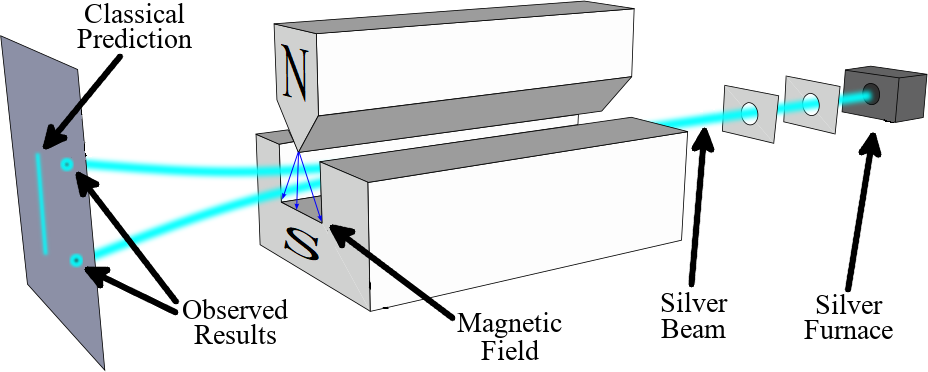
\includegraphics[width=100mm]{Chapter01/Stern-Gerlach_experiment_svg.png}
\caption[Stern-Gerlach Experiment]{The Stern-Gerlach Experiment.\protect\footnotemark}
\label{stern}
\end{figure}
\footnotetext{ Original diagram drawn by Theresa Knott. Labeling was modified for use in this dissertation. This image is licensed under the Creative Commons Attribution-Share Alike 4.0 International license. Source: https://commons.wikimedia.org/wiki/File:Stern-Gerlach\_experiment\_svg.svg.}
Now silver atoms have a property somewhat analogous to the classical notion of \emph{angular momentum}\index{angular momentum}. For instance, a spinning top has angular momentum as shown in figure \ref{spintop}. Angular momentum is a \emph{vector}\index{vector}, that is, it has direction and magnitude. In the case of a spinning top, the direction of the angular momentum would be parallel to the axis of rotation, pointing one way or the other depending on whether the rotation was clockwise or counterclockwise. The magnitude of the angular momentum would then be proportional to the \emph{angular velocity}\index{angular velocity} of the spinning top, so that the faster the top was spinning, the greater the angular velocity would be, and hence, the greater the angular momentum would be.
\begin{figure}[ht!]
\captionsetup{justification=centering}
\centering
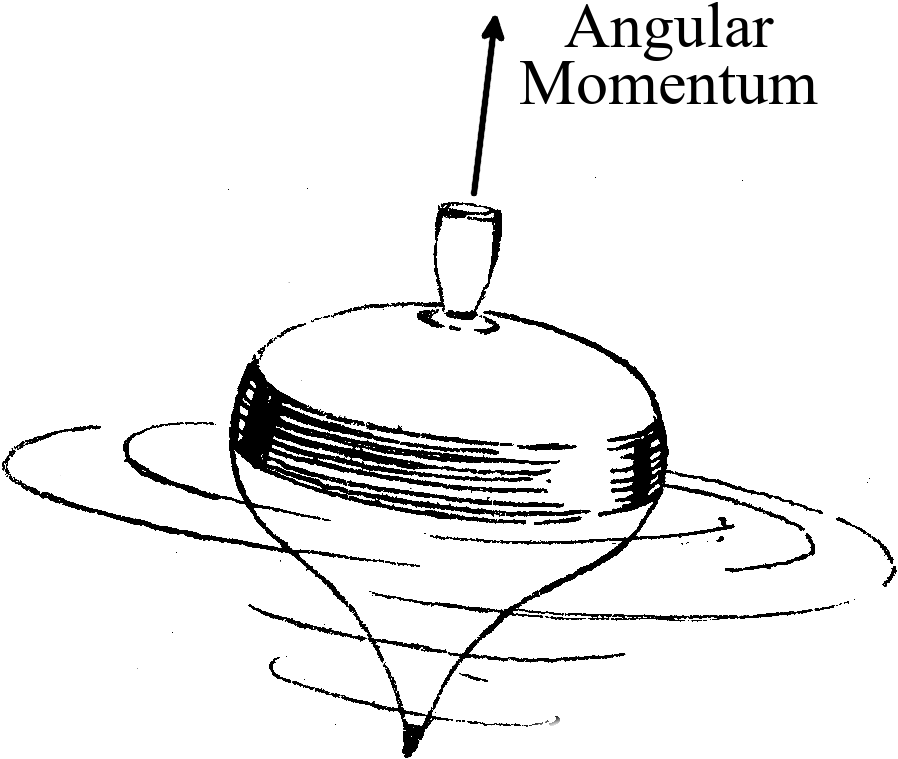
\includegraphics[width=50mm]{Chapter01/Top_(PSF)2.png}
\caption[Angular Momentum of a Spinning Top]{Angular Momentum of a Spinning Top.\protect\footnotemark}
\label{spintop}
\end{figure}

Now if we tried to understand the angular momentum of a silver atom classically, we would expect the magnetic field of the two magnets to interact with the silver atom in a way that was determined by the relative direction of the silver atom's angular momentum compared to the direction of the magnetic field.\DIFaddbegin \footnotetext{\DIFadd{Drawing by Pearson Scott Foresman, Public domain, via Wikimedia Commons. Labeling was added for use in this dissertation. Original: https://commons.wikimedia.org/wiki/
File:Top\_(PSF).png.}} \DIFaddend Since we would expect the silver atom to have an entirely random angular momentum, we would expect it to be deflected by varying degrees either up or down in the direction of the magnetic field. Thus, if a detection screen were placed beyond the two magnets which the silver atoms would hit, we would expect there to be a whole continuum of possible locations where the silver atoms would be detected. However, in reality, it is found that there are precisely two locations where the silver atoms hit the screen. It is as though the particles can spin either clockwise or anticlockwise, but that there is absolutely no variance in the angular speed at which they rotate. This is surprising. The angular momentum appears to be \textbf{quantized}\index{qunatization} in one of two directions, either parallel to the magnetic field or antiparallel \DIFdelbegin \footnotetext{\DIFdel{Drawing by Pearson Scott Foresman, Public domain, via Wikimedia Commons. Labeling was added for use in this dissertation. Original: https://commons.wikimedia.org/wiki/
File:Top\_(PSF).png.}} %DIFAUXCMD
\DIFdelend to it.\footnote{See figure \ref{antiparallel} for what is meant be antiparallel.} Corresponding to this quantization of angular momentum, we say that the atom is either in the spin up state or the spin down state with respect to the direction of the magnetic field. 
\begin{figure}[ht!]
\DIFdelbeginFL %DIFDELCMD < \captionsetup{justification=centering}
%DIFDELCMD < %%%
\DIFdelendFL \DIFaddbeginFL \captionsetup{justification=justified}
\DIFaddendFL \centering
\fbox{\begin{picture}(65,50)
   \put(0,10){\vector(1,1){30}} %% a
   \put(5,25){$\vec{a}$}

   \put(65,40){\vector(-1,-1){30}} %% -a
   \put(30,25){$-\vec{a}$}
\end{picture}}
\DIFdelbeginFL %DIFDELCMD < \vspace*{10px}
%DIFDELCMD < %%%
\DIFdelendFL \caption[Meaning of antiparallel]{Meaning of antiparallel: the arrows in opposite directions are said to be antiparallel to one another.}\label{antiparallel}
\end{figure}\\
\noindent If the direction of the magnetic field is implicitly understood, we write $\ket*{+}$ and $\ket*{-}$ for the spin up and spin down states of the atom respectively. We refer to the symbols $\ket*{+}$ %
\nomenclature{$\ket*{+}$}{Generic spin up state, \nomrefpage}%
and $\ket*{-}$ %
\nomenclature{$\ket*{-}$}{Generic spin down state, \nomrefpage}%
as \textbf{ket-vectors}\index{ket-vector}, or simply as kets. We can think of the ket $\ket*{+}$ for instance as shorthand for the proposition “the particle is in the spin up state.” If we knew this proposition to be true, we would know which of the two locations on the detection screen the particle would end up if it were to travel between the two magnets of the Stern-Gerlach apparatus. If we need to specify the spin with respect to a particular direction of the magnetic field, say in the $\uvb{a}$-direction, %
\nomenclature{$\uvb{a}$}{Unit vector in a particular direction, \nomrefpage}%
 we write the corresponding spin up and down states as $\ket*{\uvbp{a}}$ %
\nomenclature{$\ket*{\uvbp{a}}$}{Spin up state in the $\uvb{a}$-direction, \nomrefpage}%
and $\ket*{\uvbm{a}}$. %
\nomenclature{$\ket*{\uvbm{a}}$}{Spin down state in the $\uvb{a}$-direction, \nomrefpage}%
For convenience, we write $\uvbp{a}$ %
\nomenclature{$\uvbp{a}$}{The location a particle in the state $\ket*{\uvbp{a}}$ would hit the detection screen, \nomrefpage}%
and $\uvbm{a}$ %
\nomenclature{$\uvbm{a}$}{The location a particle in the state $\ket*{\uvbm{a}}$ would hit the detection screen, \nomrefpage}%
respectively for the location that the particle would hit the detection screen.  

The question then arises as to what happens when we rotate the magnetic field around the axis of the particle beam in the Stern-Gerlach experimental setup. It turns out that when we do this, the atoms are again detected in only one of two locations (see figure \ref{rotate}).
\begin{figure}[ht!]
\captionsetup{justification=justified}
\centering
\usetikzlibrary {angles, quotes, calc} 
\pgfmathsetmacro{\ang}{-20}
\begin{tikzpicture}
\tikzset{
mydot/.pic={\fill (0,0) circle (\dotsize);}}
\coordinate (a) at (0, -2.1);
\coordinate (b) at (0, 2.1);
\coordinate (o) at (0, 0);
\coordinate (c) at ($ (o)!1! \ang:(a) $);
\coordinate (d) at ($ (o)!1! \ang:(b) $);
\draw (-5, -3) rectangle (5, 3);
\draw[thick, loosely dashed]  (d) pic {mydot} node[anchor=south west]{$\uvbp{b}$} -- (o) -- (b) pic {mydot} node[anchor=south ]{$\uvbp{a}$} pic [draw=black!50!black, solid, fill=black!10, angle radius=15mm, "$\theta$"] {angle = d--o--b}; 
\draw[thick, loosely dashed] (a) pic {mydot} node[anchor=north ]{$\uvbm{a}$} -- (o) -- (c) pic {mydot} pic {mydot} node[anchor= east]{$\uvbm{b}$};
\fill (o) circle (\dotsize);

\draw[thick, solid, -stealth] (-2,0) -- (-0.2,0);
\node[text width=2cm, align=center] at (-3.2,0) {\footnotesize Beam center  of  the  silver atoms};
\node[draw] at (3,-2){Detection Screen};
\end{tikzpicture}
\DIFdelbeginFL %DIFDELCMD < \vspace*{10px}
%DIFDELCMD < %%%
\DIFdelendFL \caption[Locations of detections on detection screen]{Locations of detections before and after rotating the magnetic field by an angle $\theta$. Before rotation, the particles can be detected at either location $\uvbp{a}$ or location $\uvbm{a}$. After the rotation, particles can be detected at either location $\uvbp{b}$ or $\uvbm{b}$. }
\label{rotate}
\end{figure}
\\ \noindent
So suppose we knew the particle was in a spin state such that it was on course to arrive at location $\uvbp{a}$ because we had previously directed it through another magnetic field in the $\uvb{a}$-direction. For example, see figure \ref{knownspin} for how this might be done.
\begin{figure}[ht!]
\captionsetup{justification=centering}
\centering
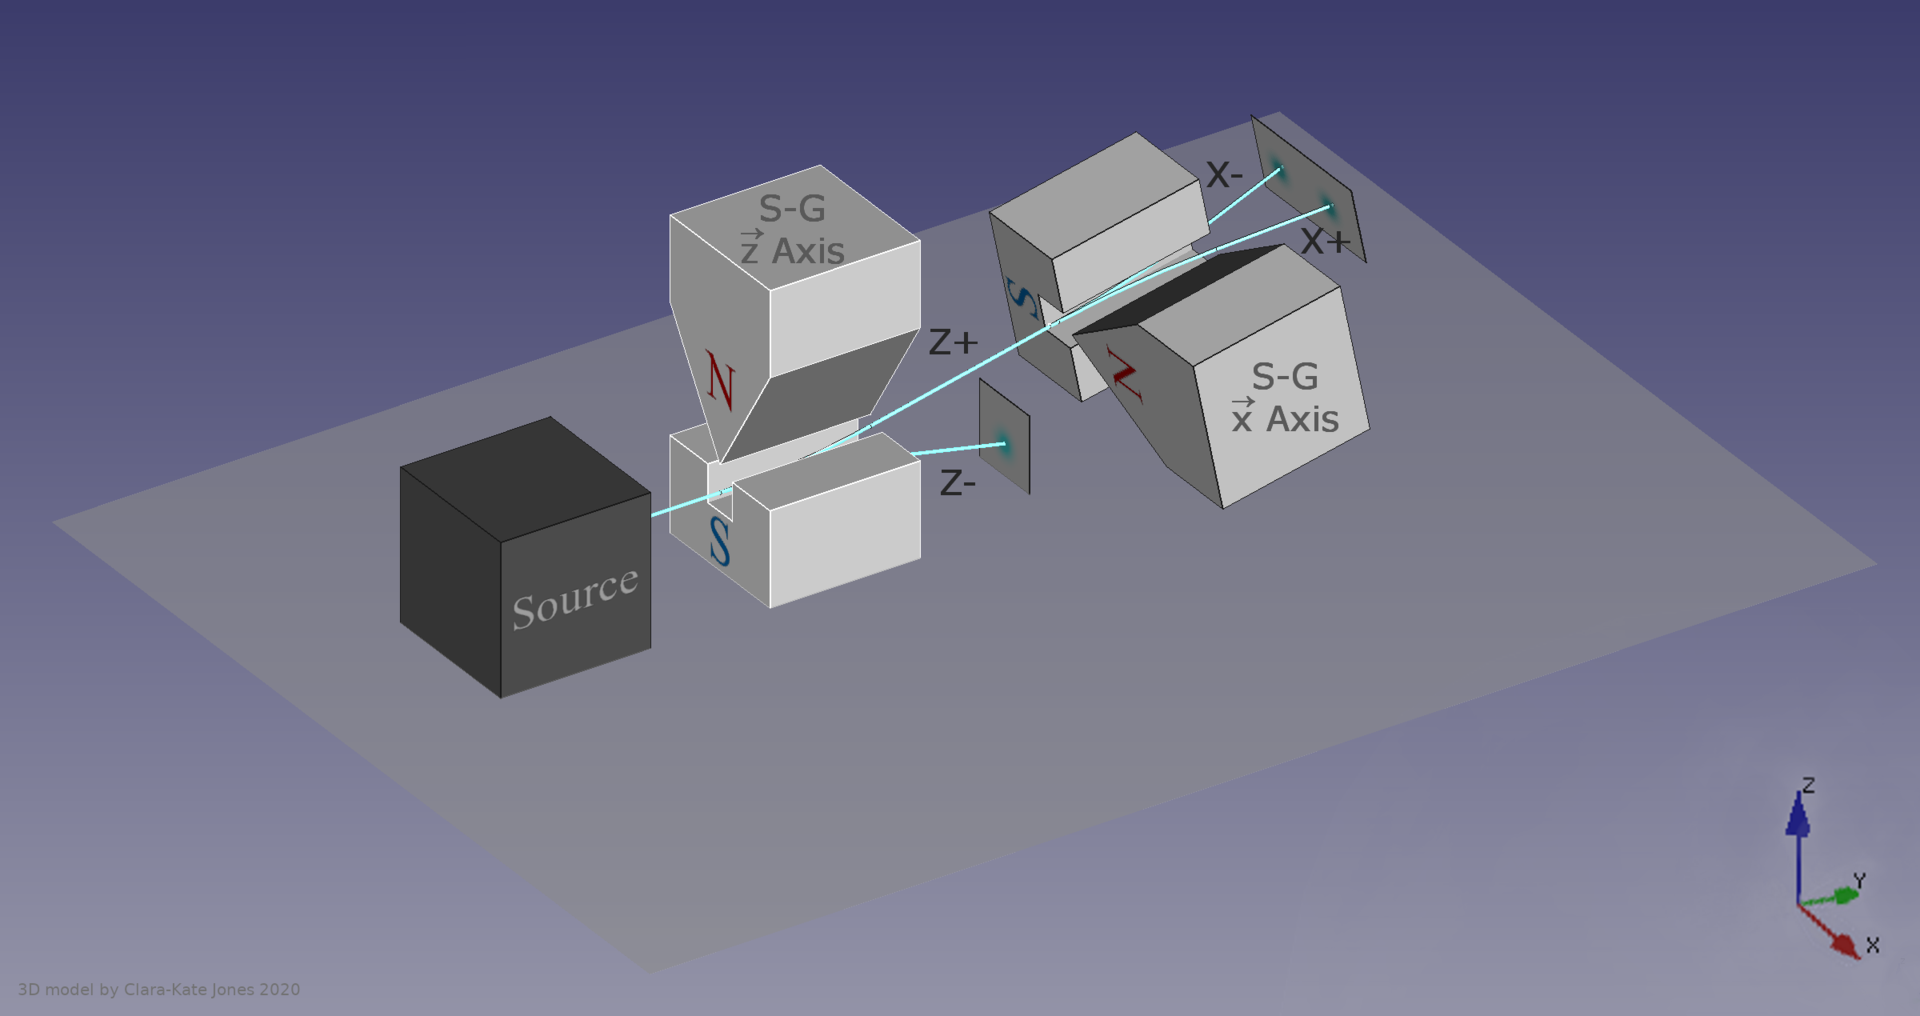
\includegraphics[width=100mm]{Chapter01/1920px-Stern-Gerlach_Analyzer_Sequential_Series_E2v.png}
\DIFdelbeginFL %DIFDELCMD < \vspace*{10px}
%DIFDELCMD < %%%
\DIFdelendFL \caption[Two Stern-Gerlach experiments in sequence]{Two Stern-Gerlach experiments in sequence. By directing the beam of particles through one magnetic field first, the particles emerging in one of the two beams will be in a known spin state before they enter the second magnetic field.\protect\footnotemark}
\label{knownspin}
\DIFaddbeginFL \vspace{12.96pt}
\DIFaddendFL \end{figure}
\DIFdelbegin \footnotetext{\DIFdel{Diagram by MJasK. This file is licensed under the Creative Commons Attribution-Share Alike 4.0 International license. Source: https://commons.wikimedia.org/wiki/File:Stern-Gerlach\_Analyzer\_Sequential\_Series\_E2.png. }} %DIFAUXCMD
\DIFdelend In this experimental setup, the second magnetic field has been rotated by an angle of $90^\circ$ with respect to the first magnetic field. But suppose we just rotated the second magnetic field by a very small angle $\theta$ with respect to the first magnetic field. Then we would expect the particle now to arrive at a location  $\uvbp{b}$ close by to $\uvbp{a}$ as shown in figure \ref{rotate}. And this is what we notice experimentally for the most part. However, occasionally, the particle will arrive at location $\uvbm{b}$. The frequency\DIFaddbegin \footnotetext{\DIFadd{Diagram by MJasK. This file is licensed under the Creative Commons Attribution-Share Alike 4.0 International license. Source: https://commons.wikimedia.org/wiki/File:Stern-Gerlach\_Analyzer\_Sequential\_Series\_E2.png. }}  \DIFaddend of this occurrence becomes less and less the less and less the magnetic field is rotated (i.e. the smaller $\theta$ is), so that if the magnetic field is not rotated at all, i.e. $\theta=0$, the particle will always arrive at location $\uvbp{a}$. 
To capture the probabilistic nature of these outcomes, we use the bra-ket notation. Thus, if $\ket*{\psi}$ stands for either the $\ket*{\uvbp{a}}$ or the $\ket*{\uvbm{a}}$-state, and $\ket*{\chi}$ stands for either the $\ket*{\uvbp{b}}$ or the $\ket*{\uvbp{b}}$-state, then we define the bra-ket $\ip*{\psi}{\chi}\in\mathbb{C}$  %
\nomenclature{$\ip*{\psi}{\chi}$}{The bra-ket of two states $\ket*{\psi}$ and $\ket*{\chi}$, \nomrefpage} %
to be a complex number\footnote{Regarding the set of complex numbers $\mathbb{C}$, %
\nomenclature{$\mathbb{C}$}{The set of complex numbers, \nomrefpage}%
we will use the notation $i=\sqrt{-1}$. %
\nomenclature{$i$}{The square root of $-1$, $\sqrt{-1}$, \nomrefpage}%
Complex conjugation will be denoted by an overline so that $\overline{x+iy}=x-iy$ %
\nomenclature{$\overline{z}$}{The complex conjugate of a complex number $z$, \nomrefpage}% 
for real numbers $x$ and $y$. The modulus of a complex number $z=x+iy$ will then be given by $\abs{z}=\sqrt{z\overline{z}}=\sqrt{x^2+y^2}.$ %
\nomenclature{$\abs{z}$}{The magnitude of the complex number $z$, \nomrefpage}%
Since the defining property of  $\ip*{\psi}{\chi}$ is that $\abs*{\ip*{\psi}{\chi}}^2$ is the probability that the particle will be found to be in state $\ket*{\psi}$ given that we know that the particle is in state $\ket*{\chi}$, we have to choose an arbitrary phase to fully determine $\ip*{\psi}{\chi}$. } that satisfies the \textbf{Born Rule}\index{Born Rule},\label{bornrule} namely the rule that $\abs*{\ip*{\psi}{\chi}}^2$ is the probability that the particle will be found to be in state $\ket*{\psi}$ given that we know that the particle is in state $\ket*{\chi}$. For example, if $\abs*{\ip*{\psi}{\chi}}^2=\frac{1}{4},$ and we performed the experiment a thousand times with the particle initially prepared in the $\ket*{\chi}$-state, then we would expect the particle to be found in the $\ket*{\psi}$-state in around 250 runs of the experiment. Given the Born Rule, we  would thus expect $\abs*{\ip*{\uvbm{a}}{\uvbp{a}}}^2$ to be $0$, from which it will follow that $\ip*{\uvbm{a}}{\uvbp{a}}$ has to be $0$. The Born Rule also implies that $\abs*{\ip*{\uvbp{a}}{\uvbp{a}}}^2=1$. We will also insist that $\ip{\psi}{\chi}=\overline{\ip{\chi}{\psi}}$,\footnote{Note that this condition implies time symmetry: the probability a particle transitions from a state $\ket*{\chi}$ to a state $\ket*{\psi}$ will be the same as the probability a particle transitions from the state $\ket*{\psi}$ to the state $\ket*{\chi}$. This is in accord with the observation that closed quantum systems are symmetric on time-reversal. A more precise formulation of this statement is given by the CPT theorem e.g. see \cite[244]{WeinbergSteven1995Tqto}. This might at first seem surprising in the light of the fact that phenomena such as radioactive decay are not obviously time-symmetric. However, it turns out that this time asymmetry results from the quantum system not being closed. For more details, see \cite{Pascazio2013}.}  from which it will follow that $\ip*{\uvbp{a}}{\uvbp{a}}$ is a real number of modulus $1$ (i.e. $+1$ or $-1$). By convention, we choose $\ip*{\psi}{\chi}$  such that $\ip*{\psi}{\psi}$ is a real and positive number, in which case we must have $\ip*{\uvbp{a}}{\uvbp{a}}=1$.
If we now rotate the magnetic field by an angle $\theta$ as indicated in figure \ref{rotate}, the particle will be detected either at location $\uvbp{b}$ or location $\uvbm{b}$. We can then ask the question “given that the particle is in state $\ket*{\uvbp{a}}$, what is the probability that the particle will be found to be in state $\ket*{\uvbp{b}}$?” According to the notation discussed above, this probability will be $|\ip*{\uvbp{b}}{\uvbp{a}}|^2$ where $\ip*{\uvbp{b}}{\uvbp{a}}$ is a complex number such that $\ip*{\uvbp{b}}{\uvbp{a}}=1$ when $\theta =0$ and $\ip*{\uvbp{b}}{\uvbp{a}}=0$ when $\theta=180\degree.$ We would likewise expect $\ip*{\uvbp{b}}{\uvbm{a}}=0$ when $\theta =0$ and $\ip*{\uvbp{b}}{\uvbm{a}}=1$ when $\theta=180\degree.$ Since $\cos 0\degree = \sin 90\degree = 1$ and $\cos 90\degree = \sin 0\degree = 0$, we might guess that in general $\abs*{\ip*{\uvbp{b}}{\uvbp{a}}}=\abs*{\cos(\theta/2)}$ and  $\abs*{\ip*{\uvbp{b}}{\uvbm{a}}}=\abs*{\sin(\theta/2)}.$\footnote{Besides this guess being correct for angles such as $0\degree$ and $180\degree$, a further reason for thinking this is a good guess follows from the fact that since a particle in the $\ket*{\uvbp{b}}$-state must be measured to be  in either the $\ket*{\uvbp{a}}$-state or the $\ket*{\uvbm{a}}$-state when measured along the $\uvb{a}$-axes, from the Born Rule we must have 
\DIFdelbegin \begin{displaymath} \DIFdel{\abs*{\ip*{\uvbp{b}}{\uvbp{a}}}^2+\abs*{\ip*{\uvbp{b}}{\uvbm{a}}}^2=1.}\end{displaymath}%DIFAUXCMD
\DIFdelend \DIFaddbegin \begin{equation*}
 \DIFadd{\abs*{\ip*{\uvbp{b}}{\uvbp{a}}}^2+\abs*{\ip*{\uvbp{b}}{\uvbm{a}}}^2=1.
}\end{equation*}\DIFaddend 
But for any angle $\theta$ we also have 
\DIFdelbegin \begin{displaymath}\DIFdel{\abs*{\cos(\theta/2)}^2+\abs*{\sin(\theta/2)}^2=1,}\end{displaymath}%DIFAUXCMD
\DIFdelend \DIFaddbegin \begin{equation*}
\DIFadd{\abs*{\cos(\theta/2)}^2+\abs*{\sin(\theta/2)}^2=1,
}\end{equation*}\DIFaddend 
and so setting $\abs*{\ip*{\uvbp{b}}{\uvbp{a}}}=\abs*{\cos(\theta/2)}$
and  $\abs*{\ip*{\uvbp{b}}{\uvbm{a}}}=\abs*{\sin(\theta/2)}$
is consistent with these two equations.} 
Experimentation shows us that this guess is correct.
This suggests that we can express the state $\ket*{\uvbp{b}}$ in terms of the states $\ket*{\uvbp{a}}$ and $\ket*{\uvbm{a}}$. We thus suppose that 
\begin{subequations}\label{vectoradd}
\begin{align}
\ket*{\uvbp{b}}&=\alpha\ket*{\uvbp{a}}+\beta\ket*{\uvbm{a}}\label{vectoradd1}\\
\ket*{\uvbm{b}}&=\bar{\alpha}\ket*{\uvbm{a}}-\bar{\beta}\ket*{\uvbp{a}}\label{vectoradd2}
\end{align} 
\end{subequations}
\DIFaddbegin \vspace{\alignspace pt}\newline
\DIFaddend for complex numbers $\alpha, \beta \in \mathbb{C}$ such that $|\alpha|^2+|\beta|^2=1$, and we suppose that the bra-ket has the \textbf{linearity}\index{linearity}\label{linearity} property so that  $\ip*{\psi}{\uvbp{b}}=\alpha\ip*{\psi}{\uvbp{a}}+\beta\ip*{\psi}{\uvbm{a}}$ and $\ip*{\psi}{\uvbm{b}}=\bar{\alpha}\ip*{\psi}{\uvbm{a}}-\bar{\beta}\ip*{\psi}{\uvbp{a}}$ for any state $\ket*{\psi}$. Then  it will follow that  $\ip*{\uvbp{b}}{\uvbm{b}}=0,$\footnote{To see this, by putting $\ket*{\psi}=\ket*{\uvbp{b}}$, we will have $\ip*{\uvbp{b}}{\uvbm{b}}=\bar{\alpha}\ip*{\uvbp{b}}{\uvbm{a}}-\bar{\beta}\ip*{\uvbp{b}}{\uvbp{a}}$ by equation (\ref{vectoradd2}). Since  $\ip*{\uvbp{b}}{\uvbm{a}}=\overline{\ip*{\uvbm{a}}{\uvbp{b}}}$ we have $\ip*{\uvbp{b}}{\uvbm{a}}=\bar{\beta}$ by equation (\ref{vectoradd1}), and likewise, since $\ip*{\uvbp{b}}{\uvbp{a}}=\overline{\ip*{\uvbp{a}}{\uvbp{b}}}$, we have $\ip*{\uvbp{b}}{\uvbp{a}}=\bar{\alpha}.$  Therefore,  $\ip*{\uvbp{b}}{\uvbm{b}}=\overline{\alpha}\overline{\beta}-\overline{\beta}{\overline{\alpha}}=0.$}  and that $\ip*{\uvbp{b}}{\uvbp{b}}=\ip*{\uvbm{b}}{\uvbm{b}} = 1.$\footnote{To see this, by putting $\ket*{\psi}=\ket*{\uvbp{b}}$ and using equation (\ref{vectoradd1}), we will have $\ip*{\uvbp{b}}{\uvbp{b}}=\alpha\ip*{\uvbp{b}}{\uvbp{a}}+\beta\ip*{\uvbp{b}}{\uvbm{a}}=\alpha\overline{\alpha}+\beta\overline{\beta}=\abs{\alpha}^2+\abs{\beta}^2=1.$ By a similar calculation, we also see $\ip*{\uvbp{b}}{\uvbp{b}}=1$.}  
If we then put  $\alpha=\cos(\theta/2)$ and $\beta=\sin(\theta/2)$, it will follow that $\abs*{\ip*{\uvbp{b}}{\uvbp{a}}}=\abs*{\cos(\theta/2)}$ and  $\abs*{\ip*{\uvbp{b}}{\uvbm{a}}}=\abs*{\sin(\theta/2)},$ \DIFdelbegin \footnote{\DIFdel{To satisfy these criteria, $\alpha$ and $\beta$ are only determined up to rotation by a complex number. Rotating a complex number $z\in\mathbb{C}$ just means multiplying it by a complex number $\lambda$ of modulus $1$ (i.e. $\abs{\lambda}=1$) to get $\lambda z$. We would need to take into account this rotation factor if we considered the three-dimensional situation. Then, without loss of generality, $\alpha=\cos(\theta/2)$ and $\beta=e^{i\phi}\sin(\theta/2)$ where $\theta$ and $\phi$ are the polar and azimuthal angles respectively.}} %DIFAUXCMD
\addtocounter{footnote}{-1}%DIFAUXCMD
\DIFdelend and so with these values for $\alpha$ and $\beta$ we will \DIFdelbegin \DIFdel{have
}\DIFdelend \DIFaddbegin {\interfootnotelinepenalty\DIFadd{=10000 have}\footnote{\DIFadd{To satisfy these criteria, $\alpha$ and $\beta$ are only determined up to rotation by a complex number. Rotating a complex number $z\in\mathbb{C}$ just means multiplying it by a complex number $\lambda$ of modulus $1$ (i.e. $\abs{\lambda}=1$) to get $\lambda z$. We would need to take into account this rotation factor if we considered the three-dimensional situation. Then, without loss of generality, $\alpha=\cos(\theta/2)$ and $\beta=e^{i\phi}\sin(\theta/2)$ where $\theta$ and $\phi$ are the polar and azimuthal angles respectively.}}  
\DIFaddend \begin{subequations}\label{spintrans}
\begin{align}
\ket*{\uvbp{b}}&= \cos(\theta/2)\ket*{\uvbp{a}}+\sin(\theta/2) \ket*{\uvbm{a}},\label{spintrans1}\\
\ket*{\uvbm{b}}&= \cos(\theta/2)\ket*{\uvbm{a}}-\sin(\theta/2) \ket*{\uvbp{a}}.\label{spintrans2}
\end{align}
\end{subequations}\DIFaddbegin }
\vspace{\alignspace pt}\newline
\DIFaddend % flatex input end: [Chapter01/Stern-Gerlach.tex]

%\usepackage[inline]{showlabels}
% flatex input: [Chapter01/EPR.tex]
\section{The Copenhagen Interpretation and the EPR-Bohm Paradox\DIFdelbegin %DIFDELCMD < \label{eprsec}%%%
\DIFdelend }\DIFaddbegin \label{eprsec}
\DIFaddend Given the equations (\ref{spintrans1}) and (\ref{spintrans2}) that  relate the states $\ket*{\uvbpm{a}}$ and $\ket*{\uvbpm{b}}$ to each other, we can calculate probabilities such as the probability a particle will be measured to be in the $\ket*{\uvbp{a}}$-state given that it is in the $\ket*{\uvbp{b}}$-state. There however arises the question of what the physical meaning of one of these states is. Clearly, the $\ket*{\uvbp{b}}$-state says something about the spin of a particle; but is this a complete description of the particle's spin state? For the $\ket*{\uvbp{b}}$-state only tells us what the outcome of a spin measurement would be along one particular axis $\uvb{b}$. For a spin measurement along another axis $\uvb{a}\neq\pm\uvb{b}$, $\ket*{\uvbp{b}}$ only tells us the probabilities (via equation (\ref{spintrans1}) and the Born Rule) that the measurement outcome would be $\ket*{\uvbp{a}}$ or $\ket*{\uvbm{a}}$ -- but the $\ket*{\uvbp{b}}$-state doesn't determine either of these outcomes. So we want to know whether this indetermination of the measurement outcome along the $\uvb{a}$-axis is merely a reflection of our lack of knowledge of a more complete specification of the particle's spin state, or alternatively, whether the  $\ket*{\uvbp{b}}$-state is a complete description of the spin state of the particle so that there is no fact of the matter about what spin state the particle would be found to be in along the $\uvb{a}$-axis until a measurement of spin along the $\uvb{a}$-axis is made. 

Now Bohr and Heisenberg believed the latter to be the case. This was because their mathematical formalism of quantum physics implied that there are physical quantities of particles that couldn't be simultaneously determined. For example, their mathematical formalism is incapable of representing a particle which has a definite spin in both the $\uvb{a}$-direction and the $\uvb{b}$-direction when $\uvb{a}\neq\pm\uvb{b}.$ So when a particle that is in the $\ket*{\uvbp{b}}$-state is measured along the $\uvb{a}$-axis and is found to be in the $\ket*{\uvbp{a}}$-state, there is a so-called collapse of the $\ket*{\uvbp{b}}$-state:
\DIFdelbegin \begin{displaymath} \DIFdel{\ket*{\uvbp{b}}= \cos(\theta/2)\ket*{\uvbp{a}}+\sin(\theta/2) \ket*{\uvbm{a}}\xrightarrow{\text{Collapse!!}}\ket*{\uvbp{a}}}\end{displaymath}%DIFAUXCMD
\DIFdelend \DIFaddbegin \begin{equation*}
 \DIFadd{\ket*{\uvbp{b}}= \cos(\theta/2)\ket*{\uvbp{a}}+\sin(\theta/2) \ket*{\uvbm{a}}\xrightarrow{\text{Collapse!!}}\ket*{\uvbp{a}}
}\end{equation*}\DIFaddend 
so that after the measurement, the particle is no longer in the $\ket*{\uvbp{b}}$-state. This interpretation of the quantum state as a complete physical description in which the state collapses to another state upon measurement is known as the \textbf{Copenhagen Interpretation}\index{Copenhagen Interpretation}.

Einstein, Podolsky, and Rosen, however, strongly objected to the Copenhagen Interpretation, and they introduced their EPR paradox to explain what troubled them.\footnote{See \cite{EinsteinPodolskyRosen}.} The EPR paradox was originally expressed in terms of the position and momentum of a particle, but it was Bohm who translated the EPR paradox to the \DIFaddbegin {\interfootnotelinepenalty\DIFadd{=10000 }\DIFaddend context of spin,\footnote{e.g. see \cite[p. 29, Ch. 5 sec. 3, and Ch. 22 sec. 19]{BohmQuantumTheory}. } and this\DIFaddbegin } \DIFaddend is the version we will consider here.   

The EPR-Bohm paradox arises in the context of particle pairs known as spin singlets. A \textbf{spin singlet}\index{spin singlet} describes the state of two particles which a single particle of zero spin has decayed into. For example, a high energy \textbf{photon}\index{photon}, that is, a particle of light, can decay into a negatively charged electron, and a positively charged positron (where a \textbf{positron}\index{positron} is a fundamental particle like an electron but of opposite charge). Since spin is a conserved physical quantity, the spin of the two particles $q_A$ and $q_B$ %
\nomenclature{$q_A, q_B$}{Two particles of a spin singlet, \nomrefpage}%
of a spin singlet state must be equal and opposite when measured along the same axis, no matter what direction this axis happens to point in. The existence of spin singlet states thus raises the question of what the physical mechanism or principle is that ensures two experimenters, Alice and Bob say, will always obtain opposite spin measurement results if Alice measures the spin of particle $q_A$, and Bob measures the spin of particle $q_B$ along the same axis. There is of course no experiment that could prove that Alice and Bob will always obtain opposite spin measurements, and there are some interpretations of quantum physics such as the GRW spontaneous collapse theory\footnote{See \cite{sep-qm-collapse}.} which predict that very occasionally Alice and Bob would obtain the same spin measurement result. But in this dissertation, we will assume that all measurements are consistent with \textbf{standard quantum theory}\index{standard quantum theory}. In other words, we assume that the physical world can be described by quantum \DIFaddbegin {\interfootnotelinepenalty\DIFadd{=10000 }\DIFaddend states\footnote{In standard quantum theory, we remain agnostic as to whether a quantum state provides a complete description of the physical world, or whether it needs to be supplemented by some additional information in order to obtain a complete description.} that \DIFaddbegin } \DIFaddend evolve over time according to the Schr\"{o}dinger equation, and that the probability of a system being found to be in one state given that it is in another state will be given by the Born Rule.  In particular, under the assumption of standard quantum theory, it will follow that Alice and Bob will always obtain opposite spin results when performing measurements along the same axis of two particles in the spin singlet state. 

Now naively, one would expect that if the spin of $q_A$ were to be measured, then this would have no effect on any spin-measurement of $q_B$. This assumption is a special case of \textbf{Einstein's locality principle}\index{Einstein's locality principle}:\label{EinsteinLocalityPrinciple} For two spatially separated systems $\mathcal{S}_1$ and $\mathcal{S}_2$, %
\nomenclature{$\mathcal{S}_1, \mathcal{S}_2$}{Two spatially separated systems, \nomrefpage}%
the real factual situation of the system $\mathcal{S}_2$ should be independent of what is done to the system $\mathcal{S}_1$.\footnote{Einstein expressed this locality principle in his autobiographical notes: ``But on one supposition we should, in my opinion, absolutely hold fast: the real factual situation of the system $\mathcal{S}_2$ is independent of what is done with the system $\mathcal{S}_1$, which is spatially separated from the former.'' \cite[p. 85]{EinsteinLocality}.} This principle seemed so intuitive to Einstein, he was convinced it must be true.\footnote{\cite[449]{IsaacsonWalter2008E:hl}.} Writing to Max Born, Einstein famously said ``Physics should represent a reality in time and space, free from spooky  action at a distance.''\footnote{From a letter written March 3, 1947, \cite[155]{BornMax2005TBl:}. Quoted from \cite[450]{IsaacsonWalter2008E:hl}.} Although Einstein offered no argument in support of his principle of locality, several arguments have been proposed in its favor. For instance,  Van Laer makes the following argument: 
\begin{adjustwidth}{1cm}{}
	\begin{displayquote}
        \DIFaddbegin \singlespacing 
\DIFaddend Suppose that body $A$ is located in void space, and that body $P$ is now brought into its vicinity. If $P$ is acted on by $A$, then either $A$'s activity ``across'' the intervening space pre-existed $P$'s arrival, in which case an action existed without an object and without a correlative passion, both of which run counter to the \emph{ratio} of action; or $A$'s activity only occurred when $P$ became present to it, in which case $A$ would somehow have to have ``known'' $P$'s becoming present, which is not consonant with the nature of mere body as such.\footnote{See \cite[59-144]{LaerP.H.van1953Pp}. The quote here is from \cite[246]{Grove}, who in turn quotes a slightly modified version of Van Laer's argument found in \cite[257]{TallaricoJames1962AaaD}. Grove also appeals to the Aristotelian doctrine of hylomorphism in order to defend the principle of locality: 
	\begin{displayquote}
        \DIFaddbegin \singlespacing
        \DIFaddend What does it mean for one hylomorphic substance to act on another? It is for the one to effect accidental or (by way of the accidental) substantial change in the other. As the accidents involved are inseparable from spatiality or extension, so must be the operations which occur through them. That is to say, that the interactions of cosmic (nonintellectual) beings are in essence spatial (and therefore spatiotemporal): they involve that which characterizes the spatial as such, i.e., ``parts outside parts,'' extendedness and adjacency. For one hylomorphic being to act on another (and for that other to ``receive'' the action of the one), there must be an ontological ground or commonality which is located precisely in their spatiality; they must ``share space,'' not in violation of the principle of unilocality but along a common boundary, thereby forming a unity through relation, i.e., ``existing with respect to one another.''\end{displayquote}\DIFaddbegin \phantom{zzzzzzz}\vspace{-20pt}\DIFaddend }
\end{displayquote}
\end{adjustwidth}

Now if Einstein's locality principle holds, we would be able to attribute a state $\ket*{\alpha}_A$ to particle $q_A$, and a state $\ket*{\beta}_B$ to particle $q_B$, %
\nomenclature{$\ket*{\alpha}_A, \ket*{\beta}_B$}{The states of two particles $q_A$ and $q_B$ respectively, \nomrefpage}%
so that if Alice were to perform a Stern-Gerlach experiment on particle $q_A$ in which one of the possible outcomes was a spin state $\ket*{\alpha'}_A$, then by the Born Rule, the probability Alice would find $q_A$ to be in state $\ket*{\alpha'}_A$ would be $|\ip{\alpha'}{\alpha}_A|^2$. Likewise, if Bob were to perform a Stern-Gerlach experiment on particle $q_B$ in which one of the possible outcomes was a spin state $\ket*{\beta'}$, then the probability Bob would find $q_B$ to be in state $\ket*{\beta'}_B$ would be $|\ip{\beta'}{\beta}_B|^2$. 

Now in order to decide how to represent the joint state of the particles $q_A$ and $q_B$, we recall that  in probability theory, we say that two events $X$ and $Y$ are \textbf{statistically independent}\index{statistical independence} if and only if 
\begin{equation}\label{indep}
    P(X, Y)=P(X)P(Y)
\end{equation}
where $P(X)$ %
\nomenclature{$P(X)$}{The probability an event $X$ occurs, \nomrefpage}%
is the probability that $X$ occurs, $P(Y)$ is the probability that $Y$ occurs, and $P(X, Y)$ is the probability that both $X$ and $Y$ both occur. We define the \textbf{conditional probability}\index{conditional probability} $P(X|Y)$ %
\nomenclature{$P(X\mid Y)$}{The probability an event $X$ occurs given that the event $Y$ occurs, \nomrefpage}%
of $X$ given $Y$ to be
\begin{equation}\label{conditionaprob}
P(X|Y)= \frac{P(X, Y)}{P(Y)}.
\end{equation}
From (\ref{indep}), it is easy to see that when $X$ and $Y$ are independent with $P(Y)\neq 0$, then $P(X|Y)=P(X)$. We also say that two events $X$ and $Y$ are \textbf{conditionally independent}\index{conditional independence} given some third event $Z$ if and only if 
\begin{equation}\label{indepcond}
P(X, Y|Z)=P(X|Z)P(Y|Z)
\end{equation} where $P(X|Z)$ is the conditional probability that $X$ occurs given $Z$, $P(Y|Z)$ is the conditional probability that $Y$ occurs given $Z$, and $P(X, Y|Z)$ is the conditional probability that both $X$ and $Y$  occur given $Z$.  

Now if $q_A$ can be described by the $\ket*{\alpha}_A$-state and $q_B$ can be described by the $\ket*{\beta}_B$-state, the Born Rule implies that the conditional probability (conditioned on $q_A$ being in the $\ket*{\alpha}_A$-state and $q_B$ being in the $\ket*{\beta}_B$-state) that Alice would measure her particle to be in the state $\ket*{\alpha'}_A$ is not going to depend on $\ket*{\beta}_B$,  and so  $P(\alpha'|\alpha, \beta)=P(\alpha'|\alpha)$.\footnote{ $P(\alpha'|\alpha, \beta)$ denotes the conditional probability that $q_A$ will be measured to be in the $\ket*{\alpha'}_A$-state given that $q_A$ is in the $\ket*{\alpha}_A$-state and $q_B$ is in the $\ket*{\beta}_B$-state.} Likewise, $P(\beta'|\alpha, \beta)=P(\beta'|\beta)$. 
Therefore, if Alice and Bob's measurement outcomes are conditionally independent given the prior states of their particles, then according to (\ref{indepcond}) and the Born Rule, we would obtain the conditional probability
\begin{equation}\label{indepprob}
    P_{AB}(\alpha', \beta'|\alpha, \beta)=|\ip{\alpha'}{\alpha}_A|^2\times|\ip{\beta'}{\beta}_B|^2=|\ip{\alpha'}{\alpha}_A\ip{\beta'}{\beta}_B|^2
\end{equation}
where $P_{AB}(\alpha', \beta'|\alpha, \beta)$ is the conditional probability Alice will measure $q_A$ to be in the $\ket*{\alpha'}_A$-state and Bob will measure $q_B$ to be in the $\ket*{\beta'}_B$-state given that $q_A$ is initially in the $\ket*{\alpha}_A$-state and $q_B$ is initially in the state $\ket*{\beta}$. %
\nomenclature{$P_{AB}(\alpha', \beta'\mid\alpha, \beta)$}{The conditional probability particle $q_A$ will be found to be in state $\ket*{\alpha'}$ and particle $q_B$ will be found to be in state $\ket*{\beta'}$ given that particle $q_A$ is currently in the state $\ket*{\alpha}$ and particle $q_B$ is currently in the state $\ket*{\beta}$, see equation (\ref{indepprob}), \nomrefpage}%
This suggests that if we write $\ket*{\alpha}_A\ket*{\beta}_B$ %
\nomenclature{$\ket*{\alpha}_A\ket*{\beta}_B$}{The composite state of two particles $q_A$ and $q_B$ where particle $q_A$ is in the $\ket*{\alpha}_A$-state and particle $q_B$ is in the $\ket*{\beta}_B$-state, \nomrefpage}%
for the state of the composite system of both particles, then the bra-ket of $\ket*{\alpha'}_A\ket*{\beta'}_B$ and $\ket*{\alpha}_A\ket*{\beta}_B$ 
would be
\begin{equation}\label{innerprod}
    \prescript{}{B}{ \bra*{\beta'}}\prescript{}{A}{\ip*{\alpha'}{\alpha}}_A\ket*{\beta}_B=\ip{\alpha'}{\alpha}_A\ip{\beta'}{\beta}_B.
\end{equation} %
\nomenclature{$\ip{\alpha'}{\alpha}_A$}{The inner product of the two states $\ket*{\alpha}_A$ and $\ket*{\alpha'}_A$, \nomrefpage}%
We extend this bracket to sums of states so that it satisfies the linearity property (see page \pageref{linearity}).
However, when the particles $q_A$ and $q_B$ form a spin singlet, it will not be possible to express their joint state as $\ket*{\alpha}_A\ket*{\beta}_B$ because otherwise, according to (\ref{indepprob}), we will always be able to find a direction $\uvb{a}$ such that $P_{AB}(\uvbp{a}, \uvbp{a}|\alpha, \beta)\neq 0$, whereas in reality, the state $Z$ describing the singlet has to satisfy $P_{AB}(\uvbp{a}, \uvbp{a}|Z)=0$ for all  $\uvb{a}$.
But it turns out that the summation of states:
\begin{equation}\label{bell}
    \ket*{\Psi_{\text{Bell}}}=\frac{1}{\sqrt{2}}(\ket*{\uvbp{a}}_A\ket*{\uvbm{a}}_B-\ket*{\uvbm{a}}_A\ket*{\uvbp{a}}_B).
\end{equation} %
\nomenclature{$\ket*{\Psi_{\text{Bell}}}$}{A Bell state, see equation (\ref{bell}), \nomrefpage}%
can describe the singlet state of the two particles. We refer to the state (\ref{bell}) as a \textbf{Bell state}\index{Bell state}.\footnote{By convention, the states $ \frac{1}{\sqrt{2}}(\ket*{\uvbp{a}}_A\ket*{\uvbm{a}}_B+\ket*{\uvbm{a}}_A\ket*{\uvbp{a}}_B)$, $ \frac{1}{\sqrt{2}}(\ket*{\uvbp{a}}_A\ket*{\uvbp{a}}_B-\ket*{\uvbm{a}}_A\ket*{\uvbm{a}}_B)$, and $ \frac{1}{\sqrt{2}}(\ket*{\uvbp{a}}_A\ket*{\uvbp{a}}_B+\ket*{\uvbm{a}}_A\ket*{\uvbm{a}}_B)$ are also referred to as Bell states.} If the composite system is in the Bell state $\ket*{\Psi_{\text{Bell}}}$, then according to the Born Rule, the probability that Alice measures her particle to be in state $\ket*{\alpha}$ and Bob measures his particle to be in the state $\ket*{\beta}$ will be:
\begin{equation}
\begin{split}
    P_{AB}(\alpha, \beta|\Psi_{\text{Bell}})&=|\prescript{}{B}{ \bra*{\beta}}\prescript{}{A}{ \ip{\alpha}{\Psi_{\text{Bell}}}}|^2\\
        &=\frac{1}{2}|\ip*{\alpha}{\uvbp{a}}_A\ip*{\beta}{\uvbm{a}}_B-\ip*{\alpha}{\uvbm{a}}_A\ip*{\beta}{\uvbp{a}}_B|^2
\end{split}
\end{equation}
This means that whatever axis Bob decides to measure along, if Alice measures her particle along the $\uvb{a}$-axis, then the Born Rule predicts that she will measure the particle to be in either the $\ket*{\uvbp{a}}_A$-state or the $\ket*{\uvbm{a}}_A$-state, each with probability of $\frac{1}{2}$.\footnote{To see this, suppose Bob performs his measurement along an arbitrary axis $\uvb{b}$. Then the probability Alice measures her particle to be in the $\ket*{\uvbp{a}}$-state will be 
\begin{equation}
    \begin{split}
        P_{AB}(\uvbp{a}, \uvbp{b}|\Psi_{\text{Bell}})&+P_{AB}(\uvbp{a}, \uvbm{b}|\Psi_{\text{Bell}})= \\
        =&\frac{1}{2}\big| \ip*{\uvbp{a}}{\uvbp{a}}_A\ip*{\uvbp{b}}{\uvbm{a}}_B-\ip*{\uvbp{a}}{\uvbm{a}}_A\ip*{\uvbp{b}}{\uvbp{a}}_B\big|^2\\
        &+\frac{1}{2}\big|\ip*{\uvbp{a}}{\uvbp{a}}_A\ip*{\uvbm{b}}{\uvbm{a}}_B-\ip*{\uvbp{a}}{\uvbm{a}}_A\ip*{\uvbm{b}}{\uvbp{a}}_B\big|^2\\
        =&\frac{1}{2}\big|\ip*{\uvbp{b}}{\uvbm{a}}_B|^2+\frac{1}{2}|\ip*{\uvbm{b}}{\uvbm{a}}_B\big|^2=\frac{1}{2}
    \end{split}
\end{equation} 
where on the last line we have used the fact that 
\DIFdelbegin \begin{displaymath}\DIFdel{\ket*{\uvbm{a}}_B=\ket*{\uvbp{b}}_B\ip*{\uvbp{b}}{\uvbm{a}}_B+\ket*{\uvbm{b}}\ip*{\uvbm{b}}{\uvbm{a}}_B}\end{displaymath}%DIFAUXCMD
\DIFdelend \DIFaddbegin \begin{equation*}
\DIFadd{\ket*{\uvbm{a}}_B=\ket*{\uvbp{b}}_B\ip*{\uvbp{b}}{\uvbm{a}}_B+\ket*{\uvbm{b}}\ip*{\uvbm{b}}{\uvbm{a}}_B
}\end{equation*}\DIFaddend 
and 
\DIFdelbegin \begin{displaymath}\DIFdel{\ip*{\uvbm{a}}{\uvbm{a}}_B=1,\quad\ip*{\uvbpm{b}}{\uvbpm{b}}_B=1,\quad\text{and}\quad \ip*{\uvbpm{b}}{\uvbmp{b}}_B=0}\end{displaymath}%DIFAUXCMD
\DIFdelend \DIFaddbegin \begin{equation*}
\DIFadd{\ip*{\uvbm{a}}{\uvbm{a}}_B=1,\quad\ip*{\uvbpm{b}}{\uvbpm{b}}_B=1,\quad\text{and}\quad \ip*{\uvbpm{b}}{\uvbmp{b}}_B=0
}\end{equation*}\DIFaddend 
so that 
\DIFdelbegin \begin{displaymath}\DIFdel{|\ip*{\uvbp{b}}{\uvbm{a}}_B|^2+\ip*{\uvbm{b}}{\uvbm{a}}_B|^2=1.}\end{displaymath}%DIFAUXCMD
\DIFdelend \DIFaddbegin \begin{equation*}
\DIFadd{|\ip*{\uvbp{b}}{\uvbm{a}}_B|^2+\ip*{\uvbm{b}}{\uvbm{a}}_B|^2=1.
}\end{equation*}\DIFaddend 
} But also, the Born Rule implies that if both Alice and Bob measure their respective particles along the same $\uvb{a}$-axis, then the probability Bob will measure his particle to have the same spin as Alice's particle will be zero, and the probability that Bob measures his particle to have the opposite spin from Alice's particle will be one.\footnote{This is because the probability Alice and Bob will measure their particles to have the same spin will be 
\begin{equation*}
\begin{split}
    P_{AB}(\uvbp{a}, \uvbp{a}|\Psi_{\text{Bell}})&+P_{AB}(\uvbm{a}, \uvbm{a}|\Psi_{\text{Bell}})= \\
    =&\frac{1}{2}\big| \ip*{\uvbp{a}}{\uvbp{a}}_A\ip*{\uvbp{a}}{\uvbm{a}}_B-\ip*{\uvbp{a}}{\uvbm{a}}_A\ip*{\uvbp{a}}{\uvbp{a}}_B\big|^2\\
    &+\frac{1}{2}\big|\ip*{\uvbm{a}}{\uvbp{a}}_A\ip*{\uvbm{a}}{\uvbm{a}}_B-\ip*{\uvbm{a}}{\uvbm{a}}_A\ip*{\uvbm{a}}{\uvbp{a}}_B\big|^2=0.
\end{split}
\end{equation*}
It therefore follows that Alice and Bob will measure their particles to have different spins with probability $1$, since for any proposition $q$ and its negation $\neg q$ (e.g. $q =$ Alice and Bob measure their particles to have the same spin, and $\neg q = $ Alice and Bob measure their particles to have different spins), the sum of the probabilities of $q$ and of $\neg q$ conditioned on any other proposition $\Psi$ that has non-zero probability (e.g. the particles $q_A$ and $q_B$ are in the $\ket*{\Psi_{\text{Bell}}}$ state) must be equal to $1$, i.e. we must have $P(q|\Psi)+P(\neg q|\Psi)=1.$} 
These probabilities predicted by the Born Rule using the Bell state $\ket*{\Psi_{\text{Bell}}}$ correspond to the probabilities observed experimentally. Also note that despite the appearance of the formula (\ref{bell}), $\ket*{\Psi_{\text{Bell}}}$ is independent of the axis $\uvb{a}$. That is, for any other direction $\uvb{b}$, it can be shown that,
\begin{equation}\label{bellstate2}\frac{1}{\sqrt{2}}(\ket*{\uvbp{a}}_A\ket*{\uvbm{a}}_B-\ket*{\uvbm{a}}_A\ket*{\uvbp{a}}_B)=\frac{1}{\sqrt{2}}(\ket*{\uvbp{b}}_A\ket*{\uvbm{b}}_B-\ket*{\uvbm{b}}_A\ket*{\uvbp{b}}_B).\protect\footnotemark\end{equation}
\footnotetext{\label{bellstate2pf}To see this, using the transformation rules given in equation (\ref{spintrans}) we have 
\begin{align*}\frac{1}{\sqrt{2}}(\ket*{\uvbp{b}}\ket*{\uvbm{b}}&-\ket*{\uvbm{b}}\ket*{\uvbp{b}})\\
      &=\frac{1}{\sqrt{2}}((\cos(\theta/2)\ket*{\uvbp{a}}+\sin(\theta/2)\ket*{\uvbm{a}})(\cos(\theta/2)\ket*{\uvbm{a}}-\sin(\theta/2)\ket*{\uvbp{a}})\\
&\quad-(\cos(\theta/2)\ket*{\uvbm{a}}-\sin(\theta/2)\ket*{\uvbp{a}})(\cos(\theta/2)\ket*{\uvbp{a}}+\sin(\theta/2)\ket*{\uvbm{a}}))\\ 
&=\frac{1}{\sqrt{2}}(\cos(\theta/2)\ket*{\uvbp{a}}\cos(\theta/2)\ket*{\uvbm{a}}-\cos(\theta/2)\ket*{\uvbp{a}}\sin(\theta/2)\ket*{\uvbp{a}}\\
&\quad+\sin(\theta/2)\ket*{\uvbm{a}}\cos(\theta/2)\ket*{\uvbm{a}}-\sin(\theta/2)\ket*{\uvbm{a}}\sin(\theta/2)\ket*{\uvbp{a}}\\
&\quad-\cos(\theta/2)\ket*{\uvbm{a}}\cos(\theta/2)\ket*{\uvbp{a}}-\cos(\theta/2)\ket*{\uvbm{a}}\sin(\theta/2)\ket*{\uvbm{a}}\\
&\quad+\sin(\theta/2)\ket*{\uvbp{a}}\cos(\theta/2)\ket*{\uvbp{a}}+
\sin(\theta/2)\ket*{\uvbp{a}}\sin(\theta/2)\ket*{\uvbm{a}})\\
&=\frac{1}{\sqrt{2}}((\cos[2](\theta/2)+\sin[2](\theta/2))\ket*{\uvbp{a}}\ket*{\uvbm{a}}-(\cos[2](\theta/2)+\sin[2](\theta/2))\ket*{\uvbm{a}}\ket*{\uvbp{a}})\\
&=\frac{1}{\sqrt{2}}(\ket*{\uvbp{a}}\ket*{\uvbm{a}}-\ket*{\uvbm{a}}\ket*{\uvbp{a}}).
\end{align*}
\DIFaddbegin \DIFadd{Hence, equation (\ref{bellstate2}).}\DIFaddend }Therefore, if Alice had chosen to measure her particle along the $\uvb{b}$-axis rather than the $\uvb{a}$-axis, she would still obtain equal probabilities for finding her particle to be in either the state $\ket*{\uvbp{b}}_A$ or $\ket*{\uvbm{b}}_A$, and the same equal probabilities for Bob's measurement outcomes hold as well. 

Now although attributing the state $\ket*{\Psi_{\text{Bell}}}$ to a spin singlet successfully determines the experimentally observed probabilities for  Alice and Bob's spin measurement outcomes, this fact spells trouble for the Copenhagen interpretation. For if we stipulate that $\ket*{\Psi_{\text{Bell}}}$ is a complete description of the spin state of the spin-singlet, then assuming Alice makes her measurement first and obtains the measurement outcome $\ket*{\uvbp{a}}_A$, then as this measurement outcome is established there will be a collapse of the state
\begin{equation}\label{BellCollapse1}
\ket*{\Psi_{\text{Bell}}}=\frac{1}{\sqrt{2}}(\ket*{\uvbp{a}}_A\ket*{\uvbm{a}}_B-\ket*{\uvbm{a}}_A\ket*{\uvbp{a}}_B)\xrightarrow{\text{Collapse!!}}\ket*{\uvbp{a}}_A\ket*{\uvbm{a}}_B,
\end{equation}
whereas if Alice makes her measurement first and obtains the measurement outcome $\ket*{\uvbm{a}}_A$, there will be a state collapse
\begin{equation}\label{BellCollapse2}
    \ket*{\Psi_{\text{Bell}}}=\frac{1}{\sqrt{2}}(\ket*{\uvbp{a}}_A\ket*{\uvbm{a}}_B-\ket*{\uvbm{a}}_A\ket*{\uvbp{a}}_B)\xrightarrow{\text{Collapse!!}}\ket*{\uvbm{a}}_A\ket*{\uvbp{a}}_B.
    \end{equation}
Thus, according to the Copenhagen interpretation, prior to Alice's measurement, the real factual situation of particle $q_B$ will be indeterminate, but once Alice has made her measurement, if she obtains the outcome $\ket*{\uvbp{a}}_A$, the real factual situation of particle $q_B$ will be expressed by the determinate state $\ket*{\uvbm{a}}_B$, and if she obtains the outcome $\ket*{\uvbm{a}}_A$, the real factual situation of particle $q_B$ will be expressed by the determinate state $\ket*{\uvbp{a}}_B$. But in either case, in the state collapse that Alice brings about via her measurement, there is a violation of Einstein's locality principle.

But things get even worse when we take Einstein's theory of special relativity into consideration. For according to special relativity, the order in which Alice and Bob perform their measurements is going to depend on their respective velocities\footnote{\label{Velocityfootnote}\emph{Velocity}\index{velocity} is a vector that specifies both the speed (the velocity's magnitude) of something and its direction. In three dimensions, a three-tuple $\vb{v}=(v_x, v_y, v_z)$  %
\nomenclature{$\vb{v}$}{A vector $\vb{v}= (v_x, v_y, v_z)$ denoting a velocity, \nomrefpage}%
is needed to specify the velocity of something, where the $v_x$ component specifies how fast the thing is moving along the $x$-axis, and similarly, the $v_y$ and $v_z$ components specify how fast the thing is moving along the $y$ and $z$ axes respectively.} and on which inertial frame of reference one is in.\footnote{\label{inertialfootnote}In special relativity, an inertial frame of reference is a spacetime coordinate system $(t, x, y, z)$   %
\nomenclature{$(t, x, y, z)$}{A spacetime location where $t$ parameterizes time, and $x$, $y$, and $z$ parameterize the three dimensions of space, \nomrefpage}%
in which all objects which have no forces acting on them have trajectories that are straight lines. Thus, we can move to another inertial frame by moving to a reference frame with constant velocity $\vb{v}$ with respect to the first reference frame. In the case when $\vb{v}=(v, 0, 0)$, Einstein's theory of special relativity tells us that under such a “boost”,\index{boost} spacetime coordinates will transform as $(t,\vb{x})\rightarrow(t',x',y',z')=(\gamma\big(t - \frac{vx}{c^2}\big),\gamma(x-vt),y,z)$  %
\nomenclature{$\vb{x}$}{A vector $\vb{x}= (x, y, z)$ representing a location in three-dimensional space, \nomrefpage}%
where $c$  %
\nomenclature{$c$}{The speed of light, \nomrefpage}%
is the speed of light and $\gamma=\Big(\sqrt{1-\frac{v^2}{c^2}}\Big)^{-1}.$ For details of the derivation of this transformation, see footnote \ref{srdefivation} on page \pageref{srdefivation}.} Thus, if we are moving at one velocity, it may appear that Alice makes her measurement first meaning that Alice causes the state collapse and thus affects the state of Bob's particle, whereas if we are moving at another velocity, it may appear that Bob makes his measurement first causing the state to collapse and thus affects the state of Alice's particle. Once the collapse has occurred, there is no further collapse when the second experimenter makes his or her measurement along the same axis as the first experimenter. Thus, the thesis of the Copenhagen interpretation that it is the act of measurement that causes the state to collapse is not compatible with Einstein's theory of special relativity, for if special relativity is correct, then one and the same measurement both will and will not cause the state to collapse depending upon which frame of reference one is in.

Therefore, if one is more convinced (as most physicists are) of the truth of special relativity than the truth of the Copenhagen interpretation, then one must reject the Copenhagen interpretation.\footnote{One might still try to imagine models of reality in which special relativity and the Copenhagen interpretation are compatible. For example, here's a scenario suggested by my advisor Alexander Pruss: suppose that whenever there are two spacelike separated measurements of an entangled system of two particles, an angel flips a coin to decide which measurement collapses the system first in the causal order. Then if reality were like this, perhaps special relativity and the Copenhagen interpretation could be compatible. However, a problem with this model is that it entails the possibility of backwards in time causality. This is because according to the Copenhagen interpretation, a measurement causes the state to collapse if and only if the system being measured is in a superposition of different measurement outcomes immediately before the measurement is made. So if an angel flips a coin which determines that Alice is the person whose measurement makes the state collapse, then if we choose an inertial frame in which Bob makes his measurement before Alice, then since Bob's measurement doesn't cause the state to collapse, the state of the particle he is measuring must already be in one of the measurement outcome states. But since the angel determines that Alice makes the state collapse, this would mean that as the entangled state of both particles evolved via the Schr\"{o}dinger equation towards the time when Alice makes her measurement, Bob's particle would have to be in a superposition of possible measurement outcomes until Alice made her measurement. So for Bob not to collapse the state, the act of Alice's measurement would have to change the history of Bob's particle so that it was in a definite outcome state immediately before he made his measurement. So if one is willing to grant the possibility of backwards in time causality so that some action could change the past, then maybe special relativity and the Copenhagen interpretation are compatible. Price takes seriously the possibility of backwards causality in \cite{PriceHuw1994ANRt}. However, if one were to insist that the impossibility of backwards in time causality was an implicit assumption of special relativity and/or quantum mechanics, then at least in the model just considered here, it doesn't look like special relativity and the Copenhagen interpretation would be compatible.} Thus, in the light of the EPR-Bohm paradox we need an alternative to the Copenhagen interpretation of quantum states that can account for how the two experimenters of the paradox always obtain opposite results when they make their measurement along the same axis. The obvious approach to take is to suppose that the quantum state $\ket*{\Psi_{\text{Bell}}}$ is an incomplete description of the spin state of the two particles. This is the hidden variables approach, but as we will see shortly, this approach is also problematic. But before we consider the hidden variables approach, we will turn to what is traditionally considered to be one of the most troubling aspect of the Copenhagen interpretation, namely the possibility of scenarios exemplified by Schr\"{o}dinger's cat thought experiment.

% flatex input end: [Chapter01/EPR.tex]

%\usepackage[inline]{showlabels}
% flatex input: [Chapter01/SchrodingerCat.tex]

\section{Schr\"{o}dinger's Cat\DIFdelbegin %DIFDELCMD < \label{SchrondingersCat}%%%
\DIFdelend }\DIFaddbegin \label{SchrondingersCat}
\DIFaddend Schr\"{o}dinger's famous thought experiment was first discussed in a 1935 paper in the context of the EPR paradox and the inherent problems it raised for the Copenhagen interpretation.\footnote{For Schr\"{o}dinger's original reference to his thought experiment, see \cite{SchrondingerOrig}. For an English translation, see \cite{SchrondingerEnglish}.} According to the Copenhagen interpretation, given the Bell state 
\begin{equation}\tag{\ref{bell} revisited}
    \ket*{\Psi_{\text{Bell}}}=\frac{1}{\sqrt{2}}(\ket*{\uvbp{a}}_A\ket*{\uvbm{a}}_B-\ket*{\uvbm{a}}_A\ket*{\uvbp{a}}_B),
\end{equation}
there is no fact of the matter as to whether particle $q_A$ is spin up and particle $q_B$ is spin down (or vice versa) until an observation is made.  

Now the strange goings-on at subatomic level might not initially give us much cause for concern about the nature of reality. For one might say that although it is an interesting curiosity that facts about subatomic particles are a bit fuzzy, our observation of definite facts in everyday life should convince us that such fuzziness can be brought into focus when we zoom out from the subatomic level to the macroscopic level. That is, we might suppose that the very many indefinite things on the small scale average out to give us something definite on the large scale. However, the Schr\"{o}dinger's Cat thought experiment suggests that our confidence in there being definite facts at the macroscopic level is seriously undermined if the Copenhagen interpretation is correct. Schr\"{o}dinger himself described the scenario in his thought experiment as ridiculous\footnote{See \cite[p. 328]{SchrondingerEnglish}.} indicating that he didn't think we should doubt the definiteness of facts at the macroscopic level; rather, we should call into question the reasonableness of the Copenhagen interpretation. 

The Schr\"{o}dinger's cat thought experiment invites us to consider a scenario like the one depicted in (\ref{BellCollapse1}) and (\ref{BellCollapse2}), but instead of having two microscopic particles coupled together, we have a microscopic particle such as a radioactive atom coupled together with a macroscopic object such as a cat. Schr\"{o}dinger suggests how this might be done. A cat is enclosed in a steel chamber in which there is a Geiger counter that is directed towards a small radioactive source, so that in the course of an hour, there is a probability of $\frac{1}{2}$ that the Geiger counter will click indicating that one of the radioactive atoms has decayed, and there is a probability of $\frac{1}{2}$ that the Geiger counter doesn't click because none of the radioactive atoms decay over the course of an hour. The Geiger counter itself is hooked up to a relay such that if the Geiger counter clicks, it releases a hammer which shatters a small flask of hydrocyanic acid causing the cat to die. The two possibilities are depicted in figure \ref{deadlivecat}.
\begin{figure}[ht!]
    \captionsetup{justification=justified}
    \centering
    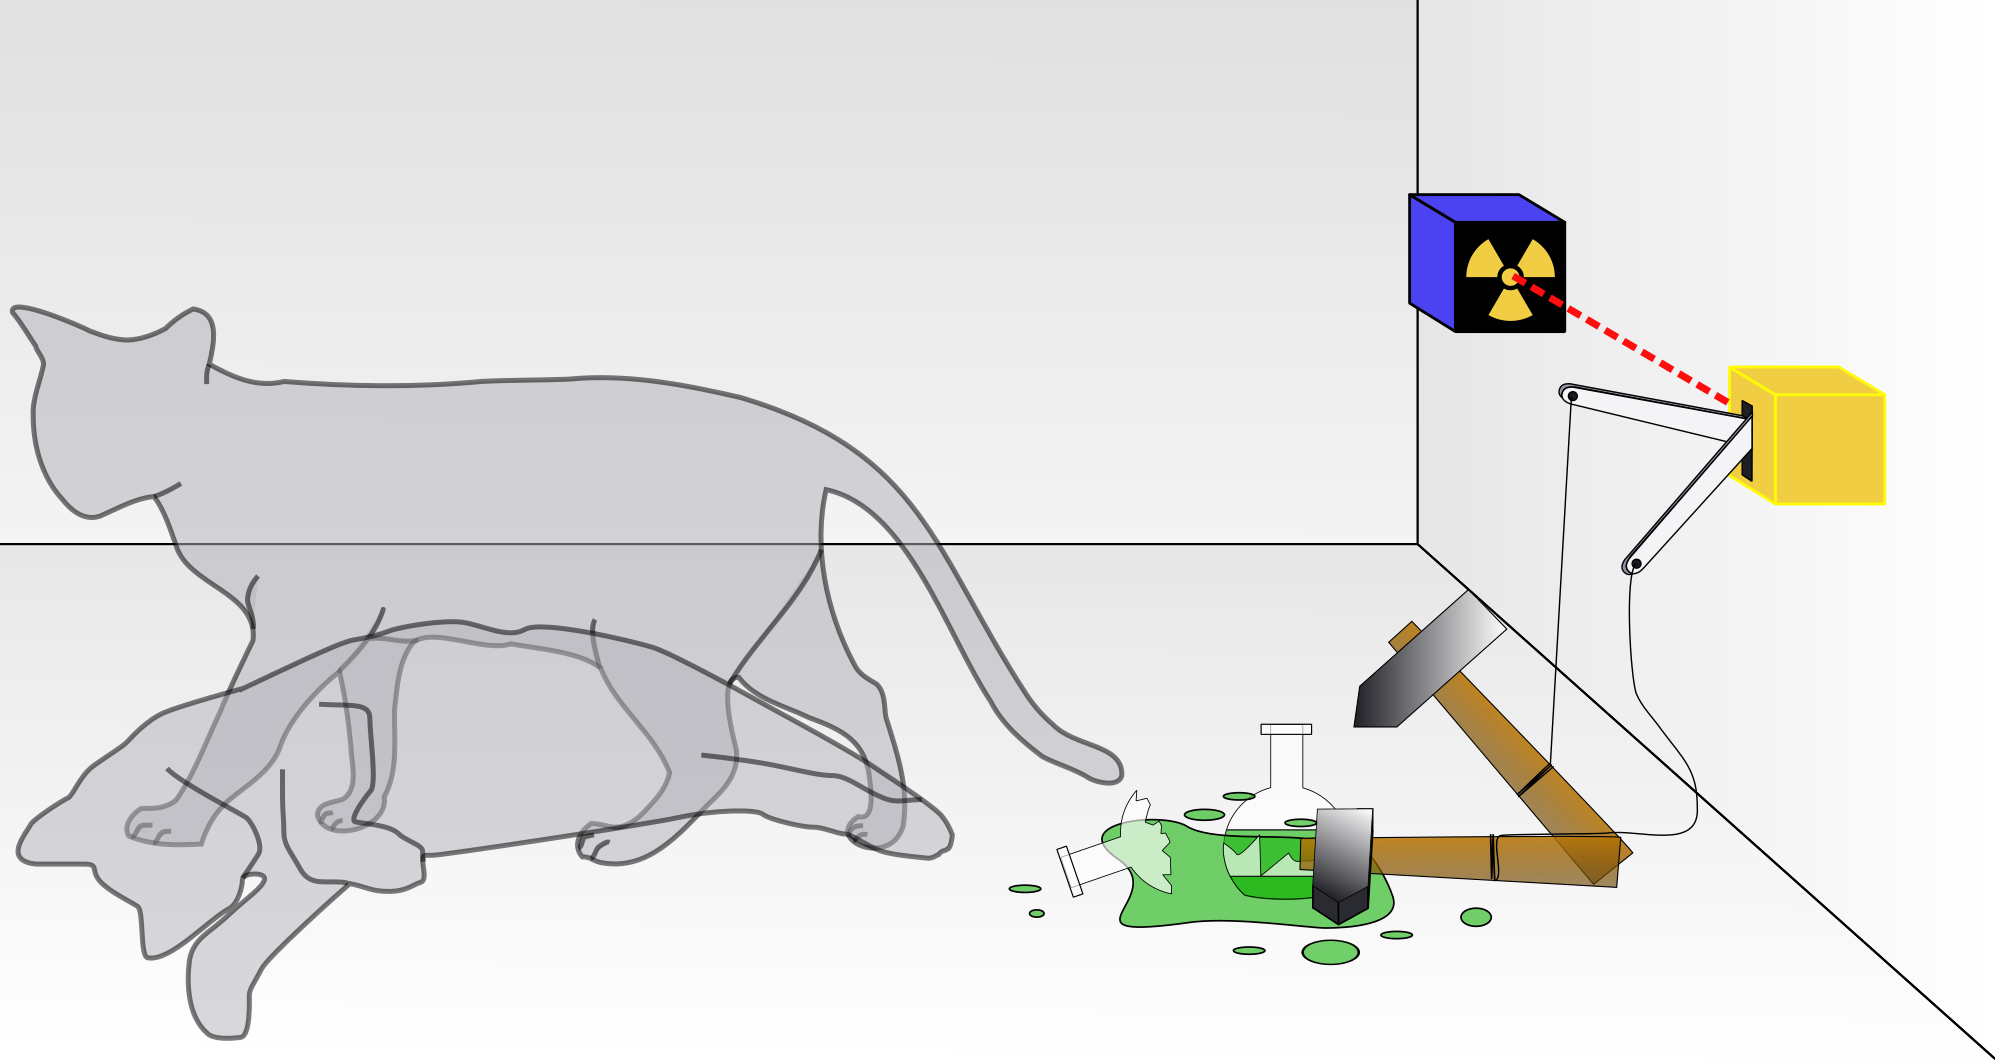
\includegraphics[width=100mm]{Chapter03/Schrodingers_cat.png}
    \caption[Depiction of Schr\"{o}dinger's cat]{A depiction of Schr\"{o}dinger's cat being both dead and alive.\protect\footnotemark}
    \label{deadlivecat}
    \end{figure}\footnotetext{ Original by Dhatfield. This image is licensed under the Creative Commons Attribution-Share Alike 3.0 Unported license. Source: https://commons.wikimedia.org/wiki/File:Schrodingers\_cat.svg\DIFaddbegin \DIFadd{.}\DIFaddend }

    
    According to the Copenhagen interpretation, the cat will only enter into a determinate state once the box is opened at the end of the hour and an observation is made. Thus, there are two possibilities analogous to (\ref{BellCollapse1}) and (\ref{BellCollapse2}): either
\begin{equation*}
    \begin{split}
\frac{1}{\sqrt{2}}\Big(\ket*{\text{No atoms decay}}\ket*{\text{Cat Alive}}&-\ket*{\text{Atom decays}}\ket*{\text{Cat Dead}}\Big)\\
&\xrightarrow{\text{Collapse!!}}\ket*{\text{No atoms decay}}\ket*{\text{Cat Alive}},
\end{split}
\end{equation*}
\DIFaddbegin \vspace{-30pt}\newline
\DIFaddend or  
\begin{equation*}
\begin{split}
\frac{1}{\sqrt{2}}\Big(\ket*{\text{No atoms decay}}\ket*{\text{Cat Alive}}&-\ket*{\text{Atom decays}}\ket*{\text{Cat Dead}}\Big)\\
&\xrightarrow{\text{Collapse!!}}\ket*{\text{Atom decays}}\ket*{\text{Cat Dead}}.
\end{split}
\end{equation*}
\DIFaddbegin \vspace{-30pt}
\newline
\DIFaddend But before the box is opened and any measurement is made, the state of the cat and the atom will not be determinate, just as in the case of the spin-singlet where the spin states of the two particles are not determined to a definite value before any measurement is made. The Schr\"{o}dinger's Cat thought experiment thus highlights that under the Copenhagen interpretation, there is no good reason to restrict  indeterminacy to the microscopic level. If there is any indeterminacy at the microscopic level, then we should expect it at the macroscopic level as well, in which case it should be possible for a cat to be in an indeterminate state of being alive and dead. It is this possibility that Schr\"{o}dinger found ridiculous. 






% flatex input end: [Chapter01/SchrodingerCat.tex]

%\usepackage[inline]{showlabels}
% flatex input: [Chapter01/HiddenVariables.tex]
\section{Hidden Variables and Bell's Inequality\DIFdelbegin %DIFDELCMD < \label{hiddenbellsection}%%%
\DIFdelend }\DIFaddbegin \label{hiddenbellsection}
\DIFaddend Given the problem with the Copenhagen interpretation that the EPR-Bohm paradox and Schr\"{o}dinger's Cat highlight, it is tempting to suppose that states such as $\ket*{\uvbp{a}}$ and $\ket*{\uvbm{a}}$ merely \DIFdelbegin \DIFdel{represents }\DIFdelend \DIFaddbegin \DIFadd{represent }\DIFaddend our limited knowledge of a more complete physical state that would also include a specification of the particle's spin state along other axes besides the $\uvb{a}$-axis. If we were to make this supposition, there would be a fact of the matter, albeit unknown to us, concerning what spin state the particle would be found to be in  were we to measure its spin along some $\uvb{b}$-axis for $\uvb{b}\neq\uvb{a}$. And  even though we might decide not to measure the spin of the particle along the $\uvb{b}$-axis, there would still be this hidden fact about the particle's spin in this direction. Furthermore, since there would be no reason to suppose there was anything special about the $\uvb{a}$ or $\uvb{b}$-axes, it would then be reasonable to suppose that there were hidden facts about what spin direction the particle would be found to be in for every possible axis orientation. This would mean that a complete description of the particle's spin state would require an infinite list of outcomes for all the possible orientations we could configure the magnetic field of our Stern-Gerlach apparatus to be in. For example, the complete spin state of a particle which according to our limited knowledge was in the $\ket*{\uvbp{b}}$-state could be depicted as $\ket*{\uvbp{a};\uvbp{b};\ldots}$ or  $\ket*{\uvbm{a};\uvbp{b};\ldots}$,  % 
\nomenclature{$\ket*{\uvbm{a};\uvbp{b};\ldots}_A$}{An example of a state of a particle $q_A$ with hidden variables specifying all the spin outcomes of every possible axis along which the spin of the particle could be measured, \nomrefpage}%
etc. where the ellipses would range over one of the two possible measurement outcomes for every other magnetic field orientation. However, because we would never in practice be able to perform all these experiments, and since only one such experiment would be needed to alter \DIFaddbegin {\interfootnotelinepenalty\DIFadd{=10000 }\DIFaddend this infinite list,\footnote{In other words, it is assumed that directly measuring the particle will involve perturbing it so that its state will change.} nearly all of the\DIFaddbegin } \DIFaddend entries in this infinite list would remain forever hidden. Hence, this would be an example of a \textbf{hidden variables}\index{hidden variables} interpretation of quantum theory.  Moreover, if we're assuming Einstein's locality principle, it follows that any changes in these hidden spin outcomes for possible measurements of a specific particle can't affect the hidden variables of any other spatially separated localized particles. Therefore, given Einstein's locality principle, it is appropriate to refer to these hidden variables as \textbf{local}\index{hidden variables!local} hidden variables.  

Now although a local hidden variables theory seems rather intuitive, in 1964, John Bell derived an inequality based on the local hidden variables theory just described.\footnote{In providing a derivation of Bell's inequality, we will follow \cite[241-249]{Sakurai}.} Moreover, it is now known that Bell's inequality can be violated \DIFaddbegin {\interfootnotelinepenalty\DIFadd{=10000 }\DIFaddend experimentally.\footnote{Aspect, Clauser and Zeilinger received the 2022 physics Nobel Prize for establishing the experimental violation of Bell's inequality. See \cite{Nobel2022}.} This\DIFaddbegin } \DIFaddend doesn't mean we must abandon all hidden variables theories. Rather it just means we need to abandon local hidden variables theories like the one Bell used in deriving his inequality.  It is nevertheless somewhat paradoxical that local hidden variables cannot account for the correlations between the measurement outcomes of spin singlets in the EPR-Bohm paradox. Local hidden variables were meant to resolve the EPR-Bohm paradox, and so the violation of Bell's inequality really heightens this paradox. Therefore, any satisfactory interpretation of quantum physics has to face up to and resolve this paradox by offering a suitable alternative to a local hidden variables theory.

In order to describe Bell's inequality, we again consider two experimenters Alice and Bob making spin measurements on a spin singlet as described in section \ref{eprsec}. So in each run of the experiment, a spin singlet consisting of two particles $q_A$ and $q_B$ will be generated with particle $q_A$ being sent to Alice who measures $q_A$'s spin in a direction of her choosing, and with particle $q_B$ being sent to Bob who measures $q_B$'s spin in a direction of his choosing.  But now, instead of describing the two particles by the state $\ket*{\Psi_{\text{Bell}}}$, we describe particles $q_A$ and $q_B$ in terms of all the spin outcomes one would obtain for every possible measurement axis in such a way that if $q_A$ is spin up with respect to an axis $\uvb{a}$, then $q_B$ would be spin down with respect to this axis. For example, if the complete spin state for $q_A$ was given by $\ket*{\Psi_A}=\ket*{\uvbp{a};\uvbp{b};\uvbm{c};\ldots}_A$, then the complete spin state for $q_B$ would be given by $\ket*{\Psi_B}=\ket*{\uvbm{a};\uvbm{b};\uvbp{c};\ldots}_B$.

We also assume that in each run of the experiment, Alice and Bob independently measure the spin of their particles along one of three possible directions $\uvb{a}$, $\uvb{b}$, and $\uvb{c}$, and that Einstein's locality principle holds. Furthermore, we assume that in each run of the experiment, the outcome of Alice's measurement will be statistically independent of any of the other measurement outcomes for different runs of the experiment, and for any of the three axes she measures along, she will get a spin up outcome or a spin down outcome with equal probability of $\frac{1}{2}.$ Likewise, we assume Bob's measurement outcomes are also similarly independent between different runs of the experiment. We also assume that the $8=2^3$ states $\ket*{\uvbpm{a};\uvbpm{b};\uvbpm{c}}_A$ exhaust all the possible states for Alice's particles that can be distinguished from one another by making one of the three possible measurement choices available. Thus, Alice can distinguish between the $\ket*{\uvbp{a};\uvbp{b};\uvbp{c}}_A$-state and the $\ket*{\uvbp{a};\uvbp{b};\uvbm{c}}_A$-state by making a measurement along the $\uvb{c}$-axis, though if she happened to make her measurement along the $\uvb{a}$ or $\uvb{b}$-axis, she wouldn't be able to distinguish between these two states. But in principle, she can distinguish between these two states if she happens to make her measurement along the right axis, in this case the $\uvb{c}$-axis. We similarly assume the states $\ket*{\uvbpm{a};\uvbpm{b};\uvbpm{c}}_B$  exhaust all the possible states for Bob's particles that he can distinguish between, and we assume that if Alice and Bob measure the particle along the same axis, they will always obtain opposite results from one another. For instance, if Alice's particle is in state $\ket*{\uvbp{a};\uvbp{b};\uvbp{c}}_A$, then Bob's particle must be in state $\ket*{\uvbm{a};\uvbm{b};\uvbm{c}}_B$. Now suppose the experiment is run $N$ times for large $N$,\footnote{$N$ has to be large since a frequentist definition of probability is being assumed.} and let $N_i$ be the number of times particle $q_A$ is in the $i$th state so that\footnote{The notation $\sum_{i=1}^8 N_i$ is shorthand for $N_1+N_2+N_3+N_4+N_5+N_6+N_7+N_8$.  %
\nomenclature{$\sum_{i=1}^8 N_i$}{Shorthand for $N_1+N_2+N_3+N_4+N_5+N_6+N_7+N_8$, \nomrefpage}%
} $N=\sum_{i=1}^8 N_i$ as shown in table \ref{hiddentable}.

      \begin{table}[ht]
      \DIFdelbeginFL %DIFDELCMD < \caption{%%%
\DIFdelendFL \DIFaddbeginFL \caption[Spin-components of particles in the hidden-variable theory]{\DIFaddendFL Spin-components of particles $q_A$ and $q_B$ in the hidden-variable theory}
      \DIFaddbeginFL \vspace{-12.96pt}
      \DIFaddendFL \centering
      \begin{tabular}{c c c} 
      \\ 
      \hline
      \textbf{Population}& \textbf{Particle} $\bm{q_A}$ & \textbf{Particle} $\bm{q_B}$ \\ [0.5ex] 
      \hline
      $N_1$ & $\ket*{\uvbp{a};\uvbp{b};\uvbp{c}}_A$ & $\ket*{\uvbm{a};\uvbm{b};\uvbm{c}}_B$ \\ 

      $N_2$ & $\ket*{\uvbp{a};\uvbp{b};\uvbm{c}}_A$ & $\ket*{\uvbm{a};\uvbm{b};\uvbp{c}}_B $\\ 

      $N_3$ & $\ket*{\uvbp{a};\uvbm{b};\uvbp{c}}_A$ & $\ket*{\uvbm{a};\uvbp{b};\uvbm{c}}_B$ \\ 

      $N_4$ & $\ket*{\uvbp{a};\uvbm{b};\uvbm{c}}_A$ & $\ket*{\uvbm{a};\uvbp{b};\uvbp{c}}_B $\\ 

      $N_5$ & $\ket*{\uvbm{a};\uvbp{b};\uvbp{c}}_A$ & $\ket*{\uvbp{a};\uvbm{b};\uvbm{c}}_B$ \\ 

      $N_6$ & $\ket*{\uvbm{a};\uvbp{b};\uvbm{c}}_A$ & $\ket*{\uvbp{a};\uvbm{b};\uvbp{c}}_B$ \\ 

      $N_7$ & $\ket*{\uvbm{a};\uvbm{b};\uvbp{c}}_A$ & $\ket*{\uvbp{a};\uvbp{b};\uvbm{c} }_B$\\ 

      $N_8$ & $\ket*{\uvbm{a};\uvbm{b};\uvbm{c}}_A$ & $\ket*{\uvbp{a};\uvbp{b};\uvbp{c}}_B$ \\ 
      \hline
      \end{tabular}
      \label{hiddentable}
      \end{table}
We define $P_{AB}(\uvbp{a},\uvbp{b})$   %
\nomenclature{$P_{AB}(\uvbp{a},\uvbp{b})$}{The probability particle $q_A$ is in the $\ket*{\uvbp{a}}$-state and particle $q_B$ is in the $\ket*{\uvbp{b}}$-state in the hidden variables interpretation, \nomrefpage}%
to be the probability that Alice measures particle $q_A$ to be at location $\uvbp{a}$ on her detection screen and Bob measures particle $q_B$ to be at location $\uvbp{b}$ on his detection screen where this probability is conditioned only on the assumption that the two particles are prepared in such a way as to guarantee Alice and Bob obtain opposite spin measurement outcomes if they perform their measurements along the same axis. We similarly define the probabilities for all other combinations of detection locations. It is relatively easy to calculate all these probabilities in terms of the values $N_i$ from table \ref{hiddentable},\footnote{e.g.  $P_{AB}(\uvbp{a},\uvbp{b})=\frac{N_3+N_4}{N},\, P_{AB}(\uvbp{a},\uvbp{c})=\frac{N_2+N_4}{N},\,P_{AB}(\uvbp{c},\uvbp{b})=\frac{N_3+N_7}{N}$.  } or alternatively by simply measuring the frequency of these different outcomes for where Alice and Bob detect their particles. Note that the values of $N_i$ will be unknown, but on the assumption that there is a fact of the matter of which states in table \ref{hiddentable} obtain, and on the assumption that the states to which the $N_i$ correspond exhaust all the possible states for Alice's and Bob's particles, we can show that\footnote{This inequality follows since 
\DIFdelbegin \begin{displaymath}\DIFdel{P_{AB}(\uvbp{a},\uvbp{b})=\frac{N_3+N_4}{N}\leq \frac{N_2+N_4+N_3+N_7}{N}=P_{AB}(\uvbp{a},\uvbp{c})+P_{AB}(\uvbp{c},\uvbp{b}).}\end{displaymath}%DIFAUXCMD
\DIFdelend \DIFaddbegin \begin{equation*}
\DIFadd{P_{AB}(\uvbp{a},\uvbp{b})=\frac{N_3+N_4}{N}\leq \frac{N_2+N_4+N_3+N_7}{N}=P_{AB}(\uvbp{a},\uvbp{c})+P_{AB}(\uvbp{c},\uvbp{b}).
}\end{equation*}\DIFaddend }
       \begin{equation}\label{bellinequality}
      P_{AB}(\uvbp{a},\uvbp{b})\leq P_{AB}(\uvbp{a},\uvbp{c})+P_{AB}(\uvbp{c},\uvbp{b}).
      \end{equation}
This inequality is known as \textbf{Bell's inequality}\index{Bell's inequality}, and it follows from Einstein's locality principle.  However, as already mentioned, when this experiment is actually performed, we can choose the three axes so that Bell's inequality is violated. Nevertheless,  it also turns out that this violation of Bell's inequality is entirely predictable if we assume that the state of the spin singlet consisting of the two particles $q_A$ and $q_B$ is given by the Bell state: 
    \begin{equation}
      \ket*{\Psi_{\text{Bell}}}=\frac{1}{\sqrt{2}}(\ket*{\uvbp{a}}_A\ket*{\uvbm{a}}_B-\ket*{\uvbm{a}}_A\ket*{\uvbp{a}}_B).
    \end{equation}

When the spin singlet is in the $\ket*{\Psi_{\text{Bell}}}$-state, it can be shown that 
      \begin{equation}\label{bellsin}
      P_{AB}(\uvbp{a},\uvbp{b})=\frac{1}{2}\sin^2(\theta/2)
      \end{equation}
where $\theta$ is the angle between the $\uvb{a}$-axis and $\uvb{b}$-axis.\footnote{To see why this is, let $P_A(\uvbp{a})$ be the probability that Alice would detect her particle at location $\uvbp{a}$ given that she is making a measurement along the $\uvb{a}$-axis, and let $P_{BA}(\uvbp{b}|\uvbp{a})$ be the probability that Bob will detect his particle at location $\uvbp{b}$ given that he is making a measurement along the $\uvb{b}$-axis and Alice has detected her particle at location $\uvbp{a}$. Given that the joint state of the particles is given by equation (\ref{bell}), $P_A(\uvbp{a})=\frac{1}{2}.$ But also note that if  Alice has detected her particle at location $\uvbp{a}$, then Bob's particle must be in state $\ket*{\uvbm{a}}$. From the Born Rule (see page \pageref{bornrule}) and equation (\ref{spintrans1}) it follows that 
      \DIFdelbegin \begin{displaymath}\DIFdel{P_{BA}(\uvbp{b}|\uvbp{a})= |\ip*{\uvbp{b}}{\uvbm{a}}_B|^2=\sin^2(\theta/2).}\end{displaymath}%DIFAUXCMD
\DIFdelend \DIFaddbegin \begin{equation*}
\DIFadd{P_{BA}(\uvbp{b}|\uvbp{a})= |\ip*{\uvbp{b}}{\uvbm{a}}_B|^2=\sin^2(\theta/2).
}\end{equation*}\DIFaddend  
Therefore, 
\DIFdelbegin \begin{displaymath}\DIFdel{P_{AB}(\uvbp{a},\uvbp{b})= P_A(\uvbp{a})P_{BA}(\uvbp{b}|\uvbp{a})=\frac{1}{2}\sin^2(\theta/2).}\end{displaymath}%DIFAUXCMD
\DIFdelend \DIFaddbegin \begin{equation*}
\DIFadd{P_{AB}(\uvbp{a},\uvbp{b})= P_A(\uvbp{a})P_{BA}(\uvbp{b}|\uvbp{a})=\frac{1}{2}\sin^2(\theta/2).
}\end{equation*}\DIFaddend } 
Then taking the angle between the $\uvb{a}$ and $\uvb{b}$-axes to be $90^\circ$, and the $\uvb{c}$-axis to be at $45^\circ$ to both the $\uvb{a}$ and $\uvb{b}$-axes, we would find that $P_{AB}(\uvbp{a},\uvbp{b})=\frac{1}{4}$ and $P_{AB}(\uvbp{a},\uvbp{c})+P_{AB}(\uvbp{c},\uvbp{b})=0.1464\ldots$, and so Bell's inequality would be violated if we assumed that the probability of each outcome is determined by the Bell state  (\ref{bell}). 

% flatex input end: [Chapter01/HiddenVariables.tex]

%\usepackage[inline]{showlabels}
% flatex input: [Chapter01/IdentifyingTheCulprit.tex]
\section{Isolating the Culprit}
Given the experimental violation of Bell's inequality, a strategy some philosophers of physics take is to reexamine the assumptions that lead to Bell's Inequality. Because of the observed violation of Bell's inequality, one of these assumptions will have to be discarded. The false assumption that is used to prove Bell's Inequality is sometimes referred to as \textbf{the culprit}\index{culprit, the}.\footnote{This is the terminology Butterfield uses following Abner Shimony. e.g. see \cite[1]{Butterfield}.} We therefore need to isolate the culprit, that is, we need to decide which assumption we should discard while keeping in mind that we wish to maintain a theory that is compatible with the experimental findings of quantum physics and special relativity.

Shimony noticed that there are two key assumptions in the proof of Bell's Inequality that might be identified as the culprit. He refers to one assumption as {Outcome Independence} (OI), %
\nomenclature{OI}{Outcome Independence, \nomrefpage}%
and to the \DIFaddbegin {\interfootnotelinepenalty\DIFadd{=10000 }\DIFaddend other assumption as {Parameter Independence} (PI).\footnote{See \cite[146-147]{Shimony86}.}\DIFaddbegin }  \DIFaddend %
\nomenclature{PI}{Parameter Independence, \nomrefpage} %  
Shimony argued that if we only denied OI, then the proof of Bell's Inequality would fail to go through. Yet by continuing to assume PI, there is a sense in which special relativity is not obviously violated. Shimony therefore thought that denying OI and assuming PI was sufficient to ensure peaceful coexistence between quantum theory and special relativity. In other words, Shimony thought OI was the culprit. 

% flatex input end: [Chapter01/IdentifyingTheCulprit.tex]

%\usepackage[inline]{showlabels}
% flatex input: [Chapter01/PI.tex]

\section{Parameter Independence\DIFdelbegin %DIFDELCMD < \label{PISec}%%%
\DIFdelend }\DIFaddbegin \label{PISec}
\DIFaddend To explain Shimony's\footnote{See \cite[146-147]{Shimony86} and \cite[7-9]{Butterfield}.}  notion of  Parameter Independence, we suppose we have an experimental setup similar to the experimental setup described in the previous section. Thus, we suppose there are two particles labeled $q_A$ and $q_B$, and that a measurement can be made on particle  $q_A$ at one location (e.g. Alice's laboratory), and a measurement can be made on particle $q_B$ at some other location (e.g. Bob's laboratory). We will assume that Alice can make a choice of one of $n$ measurements to be made. These are labeled $a_1,\ldots, a_n$.  %
\nomenclature{$a_i$}{One of Alice's measurement choices, \nomrefpage}%
For example, $a_1$ might be a measurement of $q_A$'s spin along the $z$-axis, whereas $a_2$ might be the measurement of $q_A$'s spin along an axis that is at  a $45^\circ$ angle to the $z$-axis etc. We use the variable $x$ to denote Alice's choice so that $x=a_i$ for some $i\in\{1,\ldots,n\}$. If Alice chooses to make measurement $a_i$ (i.e. $x=a_i$), the measurement outcome is labeled $A_i$,  %
\nomenclature{$A_i$}{Alice's measurement outcome when she makes the measurement choice $a_i$, \nomrefpage}%
and this outcome can take values $+1$ or $-1$. For example, Alice could use the convention in which $+1$ corresponds to a spin up outcome, and $-1$ corresponds to a spin down outcome. We will use the variable $X$ to denote the measurement outcome Alice obtains, %
\nomenclature{$X$}{A variable representing an unknown outcome for Alice's measurement, \nomrefpage}
\nomenclature{$x$}{A variable representing an unknown choice for Alice's measurement, \nomrefpage}%
so for example, if Alice chooses to make the $a_1$ measurement so that $x=a_1$ and obtains the outcome $A_1=1$, then $X=1$. Similarly, we use the notation $b_i,\, y$,  %
\nomenclature{$b_i$}{One of Bob's measurement choices, \nomrefpage}%
and  %
\nomenclature{$B_i$}{Bob's measurement outcome when he makes the measurement choice $b_i$, \nomrefpage}%
$B_i,\, Y$ %
\nomenclature{$Y$}{A variable representing an unknown outcome for Bob's measurement, \nomrefpage}
\nomenclature{$y$}{A variable representing an unknown choice for Bob's measurement, \nomrefpage}
%
to correspond to the measurement choices and measurement outcomes for Bob respectively.

We now suppose that there is a complete state $\lambda\in\Lambda$ % 
\nomenclature{$\lambda$}{A complete state describing both $q_A$ and $q_B$ that is independent of Alice and Bob's measurement choices, but that encodes all other features that would influence the corresponding measurement outcomes, \nomrefpage}
\nomenclature{$\Lambda$}{The set of $\lambda$ that describe both $q_A$ and $q_B$, \nomrefpage}%
describing both $q_A$ and $q_B$ that is independent of Alice and Bob's measurement choices, but that encodes all other features that would influence the corresponding measurement outcomes. Here, the domain $\Lambda$ of all such complete states will depend on how the two particles are prepared and the model we are assuming. We also assume that  $q_A$ and $q_B$ are initially coupled together in such a way that Alice and Bob would always get opposite results when they made their measurements in the same direction. For instance, for $n=3$, we might assume a model in which 
\begin{equation}\label{bellLambda}
\Lambda=\big\{(A_1, A_2, A_3 ,B_1, B_2, B_3):A_1,\, A_2,\, A_3=\pm1,\, B_i=-A_i\big\}.
\end{equation}
 In this case, $\lambda\in\Lambda$ would fully determine Alice and Bob's measurement outcomes along the three axes. This would be like the model described in the proof of Bell's Inequality with all the states of $\Lambda$ being described in table \ref{hiddentable} of section \ref{eprsec}. 

However, in general, we don't insist on such determinism. Rather, we suppose that given a complete state $\lambda\in\Lambda$, and given that Alice makes a measurement choice $x$ and Bob makes a measurement choice $y$, then there will be a probability $P_{\lambda,x,y}(X , Y)$ %
\nomenclature{$P_{\lambda,x,y}(X , Y)$}{The probability  Alice obtains outcome $X$ and Bob obtains outcome $Y$ given  Alice's measurement choice $x$, Bob's measurement choice $y$, and the complete state $\lambda$ describing the two particles they measure.\nomrefpage}%
representing the probability Alice gets outcome $X$ and Bob gets outcome $Y$. In deterministic models in which there are outcomes,\footnote{In chapter \ref{measprobchap}, we will consider the many-worlds interpretation which is a deterministic model in which there aren't outcomes.} $P_{\lambda,x,y}(X , Y)$ will have values restricted to either $0$ or $1$. In non-deterministic models, there will have to be some situations when $P_{\lambda,x,y}(X, Y)$ has a value strictly between $0$ and $1$. For example, if we assume the Copenhagen interpretation model, we could take $\lambda$ to be the Bell state (\ref{bell}). Then it follows from equation (\ref{bellstate2}) that as long as Alice and Bob's measurement choices $x$ and $y$ are in the same direction, then $P_{\lambda,x,y}(1,-1)=1/2$. Incidentally, we also note that equation (\ref{bellstate2}) implies the domain $\Lambda$ consists of a single state:
\begin{equation}\label{quantumLambda}
\Lambda=\Bigg\{\frac{1}{\sqrt{2}}\big(\ket*{\uvbp{a}}_A\ket*{\uvbm{a}}_B-\ket*{\uvbm{a}}_A\ket*{\uvbp{a}}_B\big)\Bigg\}.
\end{equation}

In both models (\ref{bellLambda}) and (\ref{quantumLambda}), we see that if we define
\begin{align}
P_{A, \lambda,x,y}(X)&=P_{\lambda,x,y}(X, 1)+P_{\lambda,x,y}(X, {-1}),\label{PIone}\\
P_{B, \lambda,x,y}(Y)&=P_{\lambda,x,y}(1, Y)+P_{\lambda,x,y}({-1}, Y),\label{PItwo}
\end{align}%
\DIFaddbegin \vspace{\alignspace pt}\newline
\DIFaddend \nomenclature{$P_{A, \lambda,x,y}(X)$}{The probability Alice obtains the outcome $X$ given the complete state $\lambda$ and Alice's measurement choice $x$ and Bob's measurement choice $y$, see equation (\ref{PIone}), \nomrefpage}%
then %
\nomenclature{$P_{B, \lambda,x,y}(Y)$}{The probability Bob obtains the outcome $Y$ given the complete state $\lambda$ and Alice's measurement choice $x$ and Bob's measurement choice $y$, see equation (\ref{PItwo}), \nomrefpage}% 
$P_{A,\lambda,x,y}(X)$ (which is the probability Alice gets the output $X$ regardless of what Bob's output is) is independent \DIFaddbegin {\interfootnotelinepenalty\DIFadd{=10000 }\DIFaddend of Bob's choice of measurement $y$.\DIFaddbegin \footnote{\DIFadd{To see that this is true for model (\ref{bellLambda}), it is obvious that $P_{A, \lambda,x,y}(X)=1$ or 0 regardless of what $y$ is. As for model (\ref{quantumLambda}), it is straightforward to show}\label{onehalf} \DIFadd{that $P_{A, \lambda,x,y}(X)=1/2$ and $P_{B,\lambda,x,y}(Y)=1/2$ for any $X,\, Y$. E.g. for $x=\vb{\hat{a}}$ and $y=\vb{\hat{b}}$, by (\ref{bellstate2}), we can assume the two particles are in the state 
}\begin{equation*}
\DIFadd{\ket*{\zeta}=\frac{1}{\sqrt{2}}\big(\ket*{\uvbp{b}}_A\ket*{\uvbm{b}}_B-\ket*{\uvbm{b}}_A\ket*{\uvbp{b}}_B\big).
}\end{equation*}
\DIFadd{Since the inner product on the composite system is given by  $\ip{\xi'}{\xi}=\ip{\psi'}{\psi}_A\ip{\chi'}{\chi}_B$ for $\ket*{\xi}=\ket*{\psi}_A\ket*{\chi}_B$ and $\ket*{\xi'}=\ket*{\psi'}_A\ket*{\chi'}_B$, it follows that  
}\begin{equation*}
\DIFadd{\prescript{}{A}{ \bra*{\vb{\hat{a}+}}}\prescript{}{B}{\ip*{\vb{\hat{b}\pm}}{\zeta}}=\mp\frac{1}{\sqrt{2}}\ip*{\vb{\hat{a}+}}{\vb{\hat{b}\mp}}_A.
}\end{equation*} 
\DIFadd{Therefore, by the Born Rule (see page \pageref{bornrule})
}\begin{equation*}
\DIFadd{P_{\lambda,\vb{\hat{a}},\vb{\hat{b}}}(\vb{\hat{a}+}, \vb{\hat{b}+})+P_{\lambda,\vb{\hat{a}},\vb{\hat{b}}}(\vb{\hat{a}+},\vb{\hat{b}-})=\frac{1}{2}\abs*{\ip*{\vb{\hat{a}+}}{\vb{\hat{b}-}}_A}^2+\frac{1}{2}\abs*{\ip*{\vb{\hat{a}+}}{\vb{\hat{b}+}}_A}^2.
}\end{equation*}
\DIFadd{But since
}\begin{equation*}
\DIFadd{\ket*{\vb{\hat{a}+}}_A=\ip*{\vb{\hat{b}+}}{\vb{\hat{a}+}}_A\ket*{\vb{\hat{b}+}}_A+\ip*{\vb{\hat{b}-}}{\vb{\hat{a}+}}_A\ket*{\vb{\hat{b}-}}_A
}\end{equation*}
\DIFadd{it follows that 
}\begin{equation*}
\DIFadd{\abs*{\ip*{\vb{\hat{a}+}}{\vb{\hat{b}+}}_A}^2+\abs*{\ip*{\vb{\hat{a}+}}{\vb{\hat{b}-}}_A}^2 =1. 
}\end{equation*}
\DIFadd{Therefore, 
}\begin{equation*}
\DIFadd{P_{\lambda,\vb{\hat{a}},\vb{\hat{b}}}(\vb{\hat{a}+}, \vb{\hat{b}+})+P_{\lambda,x,y}(\vb{\hat{a}+},\vb{\hat{b}-})=\frac{1}{2}.
}\end{equation*}
 \DIFadd{It therefore follows that in model (\ref{quantumLambda}), Alice's outcome is independent of Bob's measurement choice.}} \DIFaddend And likewise,\DIFaddbegin } \DIFaddend $P_{B,\lambda,x,y}(Y)$ (which is the probability Bob gets the output $Y$ regardless of what Alice's output is) is independent of Alice's choice of measurement $x$. \DIFdelbegin \footnote{\DIFdel{To see that this is true for model (\ref{bellLambda}), it is obvious that $P_{A, \lambda,x,y}(X)=1$ or 0 regardless of what $y$ is. As for model (\ref{quantumLambda}), it is straightforward to show}%DIFDELCMD < \label{onehalf} %%%
\DIFdel{that $P_{A, \lambda,x,y}(X)=1/2$ and $P_{B,\lambda,x,y}(Y)=1/2$ for any $X,\, Y$. E.g. for $x=\vb{\hat{a}}$ and $y=\vb{\hat{b}}$, by (\ref{bellstate2}), we can assume the two particles are in the state 
}\begin{displaymath}\DIFdel{\ket*{\zeta}=\frac{1}{\sqrt{2}}\big(\ket*{\uvbp{b}}_A\ket*{\uvbm{b}}_B-\ket*{\uvbm{b}}_A\ket*{\uvbp{b}}_B\big).}\end{displaymath}%DIFAUXCMD
\DIFdel{Since the inner product on the composite system is given by  $\ip{\xi'}{\xi}=\ip{\psi'}{\psi}_A\ip{\chi'}{\chi}_B$ for $\ket*{\xi}=\ket*{\psi}_A\ket*{\chi}_B$ and $\ket*{\xi'}=\ket*{\psi'}_A\ket*{\chi'}_B$, it follows that 
}\begin{displaymath}\DIFdel{\prescript{}{A}{ \bra*{\vb{\hat{a}+}}}\prescript{}{B}{\ip*{\vb{\hat{b}\pm}}{\zeta}}=\mp\frac{1}{\sqrt{2}}\ip*{\vb{\hat{a}+}}{\vb{\hat{b}\mp}}_A.}\end{displaymath}%DIFAUXCMD
%DIFDELCMD <  
%DIFDELCMD < %%%
\DIFdel{Therefore, by the Born Rule (see page \pageref{bornrule})
}\begin{displaymath}\DIFdel{P_{\lambda,\vb{\hat{a}},\vb{\hat{b}}}(\vb{\hat{a}+}, \vb{\hat{b}+})+P_{\lambda,\vb{\hat{a}},\vb{\hat{b}}}(\vb{\hat{a}+},\vb{\hat{b}-})=\frac{1}{2}\abs*{\ip*{\vb{\hat{a}+}}{\vb{\hat{b}-}}_A}^2+\frac{1}{2}\abs*{\ip*{\vb{\hat{a}+}}{\vb{\hat{b}+}}_A}^2.}\end{displaymath}%DIFAUXCMD
\DIFdel{But since
}\begin{displaymath}\DIFdel{\ket*{\vb{\hat{a}+}}_A=\ip*{\vb{\hat{b}+}}{\vb{\hat{a}+}}_A\ket*{\vb{\hat{b}+}}_A+\ip*{\vb{\hat{b}-}}{\vb{\hat{a}+}}_A\ket*{\vb{\hat{b}-}}_A}\end{displaymath}%DIFAUXCMD
\DIFdel{it follows that 
}\begin{displaymath}\DIFdel{\abs*{\ip*{\vb{\hat{a}+}}{\vb{\hat{b}+}}_A}^2+\abs*{\ip*{\vb{\hat{a}+}}{\vb{\hat{b}-}}_A}^2 =1. }\end{displaymath}%DIFAUXCMD
\DIFdel{Therefore, 
}\begin{displaymath}\DIFdel{P_{\lambda,\vb{\hat{a}},\vb{\hat{b}}}(\vb{\hat{a}+}, \vb{\hat{b}+})+P_{\lambda,x,y}(\vb{\hat{a}+},\vb{\hat{b}-})=\frac{1}{2}.}\end{displaymath}%DIFAUXCMD
%DIFDELCMD <  %%%
} %DIFAUXCMD
\addtocounter{footnote}{-1}%DIFAUXCMD
\DIFdelend In other models, however, it's possible that such independence does not hold. So to distinguish between such possibilities, we say a model satisfies \textbf{Parameter Independence}\index{Parameter Independence} (PI) \label{PIdef} if and only if $P_{A,\lambda,x,y}(X)$ is independent of $y$, and $P_{B,\lambda,x,y}(Y)$ is independent of $x$. In particular, PI holds in the model (\ref{bellLambda}) and in the Copenhagen interpretation model (\ref{quantumLambda}). In other words, PI holds if and only if (\ref{PIone}) and (\ref{PItwo}) hold for all $\lambda,$ $x,$ $y,$ $X,$ and $Y$. If PI fails to hold in a model, we say that the model satisfies \textbf{Parameter Dependence}\index{Parameter Dependence} (PD). %
\nomenclature{PD}{Parameter Dependence, \nomrefpage}%

% flatex input end: [Chapter01/PI.tex]

%\usepackage[inline]{showlabels}
% flatex input: [Chapter01/PDProblem.tex]
\section{The Problem with Parameter Dependence\DIFdelbegin %DIFDELCMD < \label{PDProb}%%%
\DIFdelend }\DIFaddbegin \label{PDProb}
\DIFaddend As is well known, special relativity implies that it is impossible to send signals faster than the speed of light. To see why this is, first recall that in order for light to travel at a constant speed regardless of how fast the source of light is traveling, it is 
necessary for clocks moving relative to an observer to run more slowly. For a proof of this fact, suppose Alice is an experimenter on earth and Bob is an experimenter on a spaceship which is travelling close to the speed of light away from the earth. We can imagine each of them having a simple clock in their possession which consists of a photon travelling back and forth between two mirrors one meter apart with a tick of the clock happening each time the photon hits one of the mirrors.  If both their clocks are parallel to each other (i.e. the line joining Alice's two mirrors is parallel to the line joining Bob's two mirrors) and perpendicular to Bob's motion with respect to Alice, then Alice would observe the distance the photon travels between each tick of Bob's clock to be longer than the distance the photon travels between each tick of her clock. Since Alice would observe both the photon of her own clock and the photon of Bob's clock to travel at the same speed, she would therefore observe Bob's clock to tick more slowly than her own clock. This means that if their clocks were originally synced when Bob left the earth, and Alice determined Bob's clock to have ticked $n_B$ times since his departure, then she would observe her own clock to have ticked $n_A=\gamma n_B$ times, where $\gamma >1$ depends on how fast Bob is moving relative to her.  

Now if Alice could send messages to Bob much faster than the speed of light, we could suppose she sends out a message to Bob when her clock has just ticked $n_A$ times. If the message was transmitted almost instantaneously, Bob would  receive the message at approximately the time when his clock had just ticked $n_A/\gamma$ times. 
But if Bob then immediately replied to Alice's message with his message also transmitting almost simultaneously, then since Bob will also notice Alice's clock ticking more slowly with respect to his own clock, he will determine that Alice receives his reply message at approximately the time when her clock reads $n_A/\gamma^2$ ticks. But since $\gamma>1$, this means that Alice will receive a reply to her message to Bob before she has sent her original message to him. This is clearly absurd. 

Using a slightly more technical argument\footnote{The more technical argument is as follows: we work in one spatial dimension and suppose that Bob is travelling away from Alice with velocity $v$ on a trajectory $(t, vt)$  in Alice's spacetime coordinates. At time $t_A$, she sends a message to Bob which travels at a velocity $v_m>v$ so that her message can catch up with Bob. Her message to Bob therefore has a trajectory $(t_A+T,v_m T)$ where $T$ is the interval of time after she has sent her message. At the time $t_{AB}$ in Alice's time coordinates when her message reaches Bob, her coordinates for Bob and her coordinates for her message location must coincide. Therefore, 
\DIFdelbegin \begin{displaymath}\DIFdel{(t_{AB}, v t_{AB})=(t_A +T_{AB}, v_m T_{AB}),}\end{displaymath}%DIFAUXCMD
\DIFdelend \DIFaddbegin \begin{equation*}
\DIFadd{(t_{AB}, v t_{AB})=(t_A +T_{AB}, v_m T_{AB}),
}\end{equation*}\DIFaddend 
where $T_{AB}$ is the time it takes for her message to reach Bob as measured by Alice. Solving for $t_{AB}$, we therefore find that Alice's clock will show the time \DIFdelbegin \begin{displaymath}\DIFdel{t_{AB}=\frac{t_A}{1-v/v_m}}\end{displaymath}%DIFAUXCMD
\DIFdelend \DIFaddbegin \begin{equation*}
\DIFadd{t_{AB}=\frac{t_A}{1-v/v_m}
}\end{equation*}\DIFaddend  at the moment Bob receives her message. But since Alice determines Bob's clock to be running more slowly than her own clock by a factor of $\gamma$, it follows that Bob's clock will show the time  
\DIFdelbegin \begin{displaymath}\DIFdel{t_B=\frac{t_A}{\gamma(1-v/v_m)}}\end{displaymath}%DIFAUXCMD
\DIFdelend \DIFaddbegin \begin{equation*}
\DIFadd{t_B=\frac{t_A}{\gamma(1-v/v_m)}
}\end{equation*}\DIFaddend  the moment he receives Alice's message. 


Now suppose Bob immediately replies to Alice's message with his message propagating back to Alice with velocity $-v_m$. In Bob's coordinates, Alice will have a trajectory $(t,-vt)$, and Bob's message to her will have a trajectory $(t_B+T, -v_m T)$. Since these two trajectories must coincide at the moment Bob's reply reaches Alice, it follows that Bob's clock will show a time $t_{BA}$ which satisfies the equation
\DIFdelbegin \begin{displaymath}\DIFdel{(t_{BA}, -v t_{BA})=(t_B+T_{BA}, -v_m T_{BA})}\end{displaymath}%DIFAUXCMD
\DIFdelend \DIFaddbegin \begin{equation*}
\DIFadd{(t_{BA}, -v t_{BA})=(t_B+T_{BA}, -v_m T_{BA})
}\end{equation*}\DIFaddend 
where $T_{BA}$ is the time it takes for Bob's message to Alice as measured by Bob. Solving for $t_{BA}$, we therefore find that Bob's clock will show the time
\DIFdelbegin \begin{displaymath}\DIFdel{t_{BA}=\frac{t_B}{1-v/v_m}}\end{displaymath}%DIFAUXCMD
\DIFdelend \DIFaddbegin \begin{equation*}
\DIFadd{t_{BA}=\frac{t_B}{1-v/v_m}
}\end{equation*}\DIFaddend 
when Alice receives Bob's reply. But since Bob determines Alice's clock to be running more slowly than his own clock by a factor of $\gamma$, it follows that Alice's clock will show the time  
\DIFdelbegin \begin{displaymath}\DIFdel{t_{AA}=\frac{t_B}{\gamma(1-v/v_m)}=\frac{t_A}{\gamma^2(1-v/v_m)^2}}\end{displaymath}%DIFAUXCMD
\DIFdelend \DIFaddbegin \begin{equation*}
\DIFadd{t_{AA}=\frac{t_B}{\gamma(1-v/v_m)}=\frac{t_A}{\gamma^2(1-v/v_m)^2}
}\end{equation*}\DIFaddend  the moment she receives Bob's reply. Now an absurdity will only arise if $t_{AA}<t_A$ since then Alice would receive a reply from Bob before she had sent her message. Thus, an absurdity will arise if both $\gamma^2(1-v/v_m)^2>1$ and $v_m> v$, where as already mentioned, the second inequality must hold in order for Alice's message to reach Bob and vice versa. Now as we will see in footnote \footreference{srdefivation}, \DIFdelbegin \begin{displaymath}\DIFdel{\gamma=\frac{1}{\sqrt{1-v^2/c^2}}.}\end{displaymath}%DIFAUXCMD
\DIFdelend \DIFaddbegin \begin{equation*}
\DIFadd{\gamma=\frac{1}{\sqrt{1-v^2/c^2}}.
}\end{equation*}\DIFaddend  A simple calculation therefore shows that the inequality $t_{AA}<t_A$ implies
\DIFdelbegin \begin{displaymath}\DIFdel{%DIFDELCMD < \label{absurdinequality}%%%
v>\frac{2v_m}{1+v_m^2/c^2}.
}\end{displaymath}%DIFAUXCMD
\DIFdelend \DIFaddbegin $$\DIFadd{\label{absurdinequality}
v>\frac{2v_m}{1+v_m^2/c^2}.
}$$\DIFaddend 
Combining this with the inequality $v<v_m$, we see that an absurdity will be possible if 
\DIFdelbegin \begin{displaymath} \DIFdel{v_m>\frac{2v_m}{1+v_m^2/c^2}}\end{displaymath}%DIFAUXCMD
\DIFdelend \DIFaddbegin \begin{equation*}
 \DIFadd{v_m>\frac{2v_m}{1+v_m^2/c^2}
}\end{equation*}\DIFaddend 
or equivalently, if $v_m>c$.} 
one can also see that an absurdity follows even when the signal transmission isn't almost instantaneous, just so long as the signal propagates faster than the speed of light. Special relativity therefore implies that it is impossible to send signals faster than the speed of light.

Now a serious problem with PD is that it suggests the possibility of superluminal signalling. In particular, if Alice happened to know what $\lambda$ was for each run of the experiment, and if Bob made the same measurement, then because the distribution of Alice's outcomes will depend on Bob's choice of measurement, with enough runs of the experiment, Alice should be able to work out what measurement Bob is making. And this should be possible even if Alice and Bob are separated by many light years. So it seems that faster than light communication could be possible. The only thing preventing such communication would be Alice's lack of knowledge of $\lambda$. 

One might still respond to this argument against PD by saying that in reality, Alice does not know anything about $\lambda$ and hence it won't be possible for Bob to send signals faster than the speed of light to Alice. However, it would nevertheless be very strange if the validity of special relativity hung on what human beings were capable of knowing rather than on the laws that actually governed physical reality itself. But even if it was metaphysically impossible for human beings to know $\lambda$, this would not 
allay the fears that adherents of special relativity would have against PD. For the real issue is not so much the possibility that Alice could translate a message that was transmitted from Bob at superluminal speed. Rather, the issue is that Bob could do something whose effect was propagated at superluminal speed. If PI fails, then superluminal propagation of effects will be possible.\label{lambdaknowledge} It's just that if Alice is to know the cause of this effect, she will need to know $\lambda$. But even if she doesn't know $\lambda$, it still seems as though some unknown effect has been transmitted to her superluminally, and with the superluminal propagation of an effect comes the possibility that an effect might occur before its cause. Such a possibility would be analogous to how Alice could receive a reply to a message from Bob before she had sent the original message to him. 
% flatex input end: [Chapter01/PDProblem.tex]

%\usepackage[inline]{showlabels}
% flatex input: [Chapter01/PIPilot.tex]

\section{Parameter Dependence in the Bohmian Interpretation}\label{PI}
One model which exhibits PD is the \textbf{Bohmian interpretation}\index{Bohmian interpretation} of standard quantum theory. In this interpretation, it is assumed that at any instant of time $t$, the particles $q_A$ and $q_B$ will have definite positions $\vb{x}_A$ and $\vb{x}_B$ %
\nomenclature{$\vb{x}_A, \vb{x}_B$}{Exact locations of particles $q_A$ and $q_B$ in the Bohmian interpretation, \nomrefpage}%
and definite momenta $\vb{p}_A$ and $\vb{p}_B$ %
\nomenclature{$\vb{p}_A, \vb{p}_B$}{Exact momenta of particles $q_A$ and $q_B$ in the Bohmian interpretation, \nomrefpage}%
respectively. But in addition to the positions and momenta of the particles, it is also assumed that there is a so-called \textbf{pilot wave}\index{pilot wave} 
\begin{equation}\label{pilotwave}
\psi(\vb{x}_A, \vb{x}_B, t)=r(\vb{x}_A, \vb{x}_B, t)e^{i S(\vb{x}_A, \vb{x}_B, t)} 
\end{equation}where $r(\vb{x}_A, \vb{x}_B, t)>0$ %
\nomenclature{$r(\vb{x}_A, \vb{x}_B, t)$}{Modulus of the pilot wave $\psi(\vb{x}_A, \vb{x}_B, t)$, \nomrefpage}% 
is the modulus of $\psi(\vb{x}_A, \vb{x}_B, t)$, %
\nomenclature{$\psi(\vb{x}_A, \vb{x}_B, t)$}{Pilot wave, \nomrefpage}%
and the real-valued function\footnote{A \emph{function}\index{function} is a mathematical object that takes an element from a set called the function's \emph{domain}\index{domain} as its input, and returns an output from a set called the function's \emph{range}\index{range}. A \emph{real-valued function}\index{function!real-valued} is a function whose range is contained within the set of real numbers. If $x$ is in the domain of a function $f$, we denote the corresponding output of the function $f$ as $f(x)$. The $\sin$ function is an example of a real-valued function whose domain is the set of real numbers and whose range is the set of real numbers between $-1$ and $1$. Some functions need to  take several mathematical objects as input to produce an output. For example, the function $S$ in equation (\ref{pilotwave}) takes two vectors $\vb{x}_A$ and $\vb{x}_B$, and a real number $t$ as input from which it produces an output denoted by $S(\vb{x}_A, \vb{x}_B, t)$.} $S(\vb{x}_A, \vb{x}_B,t )$ is %
\nomenclature{$S(\vb{x}_A, \vb{x}_B,t )$}{Phase of the pilot wave $\psi(\vb{x}_A, \vb{x}_B, t)$, \nomrefpage}%
the complex phase\footnote{The \textbf{phase}\index{phase of a complex number} of a complex number $z$ is the angle $\theta$ (in radians) such that $z=r(\cos \theta + i \sin \theta)$ where $r>0$ is a real number called the \textbf{modulus}\index{modulus of a complex number}. Since $\cos \theta + i\sin \theta=e^{i \theta}$, %
\nomenclature{$e^{i \theta}$}{Defined to be equal to $\cos \theta + i\sin \theta$, \nomrefpage}%
it follows from (\ref{pilotwave}) that $r(\vb{x}_A, \vb{x}_B, t)>0$ is the modulus of $\psi(\vb{x}_A, \vb{x}_B, t)$, and $S(\vb{x}_A, \vb{x}_B,t )$ is the phase of $\psi(\vb{x}_A, \vb{x}_B, t)$.} of $\psi(\vb{x}_A, \vb{x}_B, t).$
The time evolution of the pilot wave is deterministically governed by the Schr\"{o}dinger equation, and the phase $S(\vb{x}_A, \vb{x}_B, t )$ relates the positions $\vb{x}_A$ and $\vb{x}_B$ to the momenta $\vb{p}_A$ and $\vb{p}_B$ via the \DIFaddbegin {\interfootnotelinepenalty\DIFadd{=10000 }\DIFaddend gradient\footnote{Given a smooth function $F$ that maps a vector $\vb{x}$ to a real number $F(\vb{x})$, the \emph{gradient}\index{gradient} of $F$ at $\vb{x}$, written $\grad F(\vb{x})$ is the vector which points in the direction of the steepest ascent of $F$ at $\vb{x}$ and whose magnitude is determined by the rate of the steepest ascent at $\vb{x}$. When $F$ is a smooth function mapping two vectors $\vb{x}_A$ and $\vb{x}_B$ to a real number $F(\vb{x}_A, \vb{x}_B)$, we write $\grad_A F(\vb{x}_A, \vb{x}_B)$ for the gradient of $F$ at $\vb{x}_A$ when $F$ is just considered as a function of $\vb{x}_A$ with $\vb{x}_B$ fixed, and we write $\grad_B F(\vb{x}_A, \vb{x}_B)$ for the gradient of $F$ at $\vb{x}_B$ when $F$ is just considered as a function of $\vb{x}_B$ with $\vb{x}_A$ fixed.} of\DIFaddbegin } \DIFaddend $S$:
\begin{equation}
\vb{p}_A=\grad_A{S}(\vb{x}_A, \vb{x}_B),\qquad
\vb{p}_B=\grad_B{S}(\vb{x}_A, \vb{x}_B).
\end{equation}
In other words, %
\nomenclature{$\grad_A{S}(\vb{x}_A, \vb{x}_B)$}{Gradient of the function ${S}(\vb{x}_A, \vb{x}_B)$ with respect to the variable $\vb{x}_A$, \nomrefpage}%
if we fix $\vb{x}_B$ %
\nomenclature{$\grad_B{S}(\vb{x}_A, \vb{x}_B)$}{Gradient of the function ${S}(\vb{x}_A, \vb{x}_B)$ with respect to the variable $\vb{x}_B$, \nomrefpage}%
and consider $S$ to be just a function of $\vb{x}_A$, then the momentum $\vb{p}_A$ is in the direction and has the magnitude of the steepest ascent of $S$ considered as a function of $\vb{x}_A$. The momentum $\vb{p}_B$ is determined similarly. 

In reality, we don't know the exact positions of all the particles, but based on what we know about an experimental setup, we can average over our uncertainty and recover exactly the same predictions that standard quantum theory would make.\footnote{See \cite{BohmDavid1952A} and \cite{BohmDavid1952B}.} So for instance, our knowledge of the experimental setup above should enable us  to know that $q_A$ and $q_B$ are contained within a bounded region $V,$ %
\nomenclature{$V$}{The region particles $q_A$ and $q_B$ are confined to in the Bohmian interpretation, \nomrefpage}%
and the experimental setup should also enable us to work out the probability  $p(V_i, V_j)$ %
\nomenclature{$p(V_i, V_j)$}{The probability given our knowledge that particle  $q_A$ belongs to the region $V_i$ and particle $q_B$ belongs to the region $V_j$, \nomrefpage}%
that particle $q_A$  will be in a region $V_i$, and particle $q_B$ will be in a region $V_j,$ where the $V_i$ are small non-overlapping regions such that $V=\bigcup_iV_i$. %
\nomenclature{$V_i$}{Small non-overlapping regions whose union is $V=\bigcup_iV_i$, \nomrefpage}%
If we are interested in some physical quantity $O(\vb{x}_A, \vb{x}_B)$ %
\nomenclature{$O(\vb{x}_A, \vb{x}_B)$}{A physical quantity dependent on the locations of the particles $q_A$ and $q_B$ in the Bohmian interpretation, \nomrefpage}%
that depends on the positions $\vb{x}_A$ and $\vb{x}_B$ of the two particles, then when the regions $V_i$ are  sufficiently small so that almost everywhere,\footnote{I am using the expression ``almost everywhere'' in a measure theoretic sense to mean that the set of all points where discontinuities occur has measure $0$. The motivation for this qualification is that whilst it might seem reasonable to suppose that there could be physical quantities that are discontinuous in some places, it doesn't seem reasonable to suppose that there are physical quantities that could be pathologically discontinuous, e.g. we wouldn't expect there to be a physical quantity that took the value of $1$ unit when all the coordinates of a location were rational and a value of $2$ units when one of the coordinates was irrational. Given this qualification about $O(\vb{x}_A,\vb{x}_B)$ being continuous almost everywhere, then even though $O(\vb{x}_A,\vb{x}_B)$ could be discontinuous at some points so that there could be some  $V_i\times V_j$ cells in which $O(\vb{x}_A,\vb{x}_B)$ varied non-negligibly for $(\vb{x}_A,\vb{x}_B)\in V_i\times V_j$, it would still be the case that the sum of the $p(V_i, V_j)\max_{(\vb{x}_i,\vb{x}_j)\in V_i\times V_j}|O(\vb{x}_i,\vb{x}_j)|$ terms for such cells would be negligible. This follows from the Lebesgue-Vitali theorem that states that any bounded function on a compact interval is Riemann integrable if and only if it is continuous almost everywhere. See \cite{wiki:Riemann}.} $O(\vb{x}_i, \vb{x}_j)$ varies negligibly for any $\vb{x}_i\in V_i$ and $\vb{x}_j\in V_j$,  the average value (also known as the \textbf{expectation value}\index{expectation value!pilot wave})
\begin{equation}\label{bohmconsistency}
\ev{O}=\sum_{i,j}p(V_i, V_j)O(\vb{x}_i, \vb{x}_j)
\end{equation}
calculated %
\nomenclature{$\ev{O}$}{Expectation value of the physical quantity $O(\vb{x}_A, \vb{x}_B)$ in the Bohmian interpretation \nomrefpage}%
in the Bohmian interpretation turns out to be the same as the expectation value\footnote{See (\ref{expectation2}) for the definition of the expectation value of an observable in standard quantum theory.} for $O$ predicted by standard quantum theory.\footnote{In this explanation, I've refrained from using measure theory, but basically this explanation is saying that when we construct a measure $\mu$ on $V\times V$ based on our knowledge of the experimental setup,  $\int_{V\times V}O(\vb{x}_i, \vb{x}_j)\dd\mu$ will be the same as the expectation value for $O$ predicted by standard quantum theory. }

To see why PI fails to hold in the Bohmian interpretation, we first note that since the Bohmian interpretation makes the same predictions as standard quantum theory when averaged over all the hidden variables, the violation of Bell's inequality (\ref{bellinequality}) implies there must be some hidden variable $\lambda$ and choices of measurement directions $\bm{\hat{a}}$, $\bm{\hat{b}}$, and $\bm{\hat{c}}$ such that\DIFaddbegin \footnote{\DIFadd{To see why (\ref{bellinequality2}) holds, we consider the observable $O_{\uvbp{a},\uvbp{b}}(\vb{x}_A,\vb{x}_B)$ which returns $1$ if and only if the particle $q_A$ will end up at location $\uvbp{a}$ and particle $q_B$ will end up at location $\uvbp{b}$ as determined by the pilot wave, and otherwise  $O_{\uvbp{a},\uvbp{b}}(\vb{x}_A,\vb{x}_B)$ returns $0$. Then by (\ref{bohmconsistency}), 
}\begin{equation}\DIFadd{\label{bohmconsistency2}
P_{AB}(\uvbp{a},\uvbp{b})=\sum_{\lambda}p_{\lambda}P_{\lambda,\bm{\hat{a}},\bm{\hat{b}}}(\uvbp{a},\uvbp{b})
}\end{equation} 
\DIFadd{where $P_{AB}(\uvbp{a},\uvbp{b})$ is the probability described in section \ref{hiddenbellsection}, $\lambda$ ranges over the pairs of indices $(i,j)$ corresponding to the cell $V_i\times V_j$, $p_{\lambda}=p(V_i,V_j)$ for $\lambda=(i,j)$, and we have used the fact that  $P_{\lambda,\bm{\hat{a}},\bm{\hat{b}}}(\uvbp{a},\uvbp{b})=O_{\uvbp{a},\uvbp{b}}(\vb{x}_i,\vb{x}_j)$ for almost all $(\vb{x}_i,\vb{x}_j)\in V_i\times V_j$. Now if (\ref{bellinequality2}) is false, then for all $\lambda$, $\bm{\hat{a}}$, and $\bm{\hat{b}}$,  
}\begin{equation}\DIFadd{\label{falsebellinequality2}
P_{\lambda,\bm{\hat{a}},\bm{\hat{b}}}(\uvbp{a},\uvbp{b})\leq P_{\lambda,\bm{\hat{a}},\bm{\hat{c}}}(\uvbp{a},\uvbp{c})+P_{\lambda,\bm{\hat{c}},\bm{\hat{b}}}(\uvbp{c},\uvbp{b})
}\end{equation} \DIFadd{Therefore, since $p_{\lambda}\geq 0$, it follows that 
}\begin{equation}\DIFadd{\label{falsebellinequality3}
\sum_\lambda p_{\lambda}P_{\lambda,\bm{\hat{a}},\bm{\hat{b}}}(\uvbp{a},\uvbp{b})\leq \sum_\lambda p_{\lambda}P_{\lambda,\bm{\hat{a}},\bm{\hat{c}}}(\uvbp{a},\uvbp{c})+\sum_\lambda p_{\lambda} P_{\lambda,\bm{\hat{c}},\bm{\hat{b}}}(\uvbp{c},\uvbp{b}).
}\end{equation} 
\DIFadd{It would therefore follow from (\ref{falsebellinequality3}) and  (\ref{bohmconsistency2}) that Bell's inequality (\ref{bellinequality}) would hold. But since (\ref{bellinequality}) is experimentally violated, it is not the case that (\ref{falsebellinequality2}) holds for all $\lambda$, $\bm{\hat{a}}$, and $\bm{\hat{b}}$. Hence, there must be some $\lambda$, $\bm{\hat{a}}$, and $\bm{\hat{b}}$,  for which (\ref{bellinequality2}) holds.}}  \DIFaddend %
\nomenclature{$P_{\lambda,\bm{\hat{a}},\bm{\hat{b}}}(\uvbp{a},\uvbp{b})$}{The probability particle $q_A$ is measured to be in the $\ket*{\uvbp{a}}$-state and particle $q_B$ is measured to be in the $\ket*{\uvbp{b}}$-state given the complete state $\lambda$ of both particles, \nomrefpage}%
 \begin{equation}\label{bellinequality2}
P_{\lambda,\bm{\hat{a}},\bm{\hat{b}}}(\uvbp{a},\uvbp{b})> P_{\lambda,\bm{\hat{a}},\bm{\hat{c}}}(\uvbp{a},\uvbp{c})+P_{\lambda,\bm{\hat{c}},\bm{\hat{b}}}(\uvbp{c},\uvbp{b}).
\DIFdelbegin %DIFDELCMD < \protect\footnotemark
%DIFDELCMD < %%%
\DIFdelend \end{equation}\DIFdelbegin \footnotetext{\DIFdel{To see why this is, we consider the observable $O_{\uvbp{a},\uvbp{b}}(\vb{x}_A,\vb{x}_B)$ which returns $1$ if and only if the particle $q_A$ will end up at location $\uvbp{a}$ and particle $q_B$ will end up at location $\uvbp{b}$ as determined by the pilot wave, and otherwise  $O_{\uvbp{a},\uvbp{b}}(\vb{x}_A,\vb{x}_B)$ returns $0$. Then by (\ref{bohmconsistency}), 
}\begin{displaymath}\DIFdel{%DIFDELCMD < \label{bohmconsistency2}%%%
P_{AB}(\uvbp{a},\uvbp{b})=\sum_{\lambda}p_{\lambda}P_{\lambda,\bm{\hat{a}},\bm{\hat{b}}}(\uvbp{a},\uvbp{b})
}\end{displaymath}%DIFAUXCMD
%DIFDELCMD <  
%DIFDELCMD < %%%
\DIFdel{where $P_{AB}(\uvbp{a},\uvbp{b})$ is the probability described in section \ref{hiddenbellsection}, $\lambda$ ranges over the pairs of indices $(i,j)$ corresponding to the cell $V_i\times V_j$, $p_{\lambda}=p(V_i,V_j)$ for $\lambda=(i,j)$, and we have used the fact that  $P_{\lambda,\bm{\hat{a}},\bm{\hat{b}}}(\uvbp{a},\uvbp{b})=O_{\uvbp{a},\uvbp{b}}(\vb{x}_i,\vb{x}_j)$ for almost all $(\vb{x}_i,\vb{x}_j)\in V_i\times V_j$. Now if (\ref{bellinequality2}) is false, then for all $\lambda$, $\bm{\hat{a}}$, and $\bm{\hat{b}}$,  
}\begin{displaymath}\DIFdel{%DIFDELCMD < \label{falsebellinequality2}%%%
P_{\lambda,\bm{\hat{a}},\bm{\hat{b}}}(\uvbp{a},\uvbp{b})\leq P_{\lambda,\bm{\hat{a}},\bm{\hat{c}}}(\uvbp{a},\uvbp{c})+P_{\lambda,\bm{\hat{c}},\bm{\hat{b}}}(\uvbp{c},\uvbp{b})
}\end{displaymath}%DIFAUXCMD
%DIFDELCMD <  %%%
\DIFdel{Therefore, since $p_{\lambda}\geq 0$, it follows that 
}\begin{displaymath}\DIFdel{%DIFDELCMD < \label{falsebellinequality3}%%%
\sum_\lambda p_{\lambda}P_{\lambda,\bm{\hat{a}},\bm{\hat{b}}}(\uvbp{a},\uvbp{b})\leq \sum_\lambda p_{\lambda}P_{\lambda,\bm{\hat{a}},\bm{\hat{c}}}(\uvbp{a},\uvbp{c})+\sum_\lambda p_{\lambda} P_{\lambda,\bm{\hat{c}},\bm{\hat{b}}}(\uvbp{c},\uvbp{b}).
}\end{displaymath}%DIFAUXCMD
%DIFDELCMD <  
%DIFDELCMD < %%%
\DIFdel{It would therefore follow from (\ref{falsebellinequality3}) and  (\ref{bohmconsistency2}) that Bell's inequality (\ref{bellinequality}) would hold. But since (\ref{bellinequality}) is experimentally violated, it is not the case that (\ref{falsebellinequality2}) holds for all $\lambda$, $\bm{\hat{a}}$, and $\bm{\hat{b}}$. Hence, there must be some $\lambda$, $\bm{\hat{a}}$, and $\bm{\hat{b}}$,  for which (\ref{bellinequality2}) holds.}}%DIFAUXCMD
\DIFdel{Since }\DIFdelend \DIFaddbegin \DIFadd{Since }\interfootnotelinepenalty\DIFadd{=10000 }\DIFaddend physics in the Bohmian interpretation is deterministic, probabilities must be either $0$ or $1$. Therefore, the only way (\ref{bellinequality2}) can be satisfied is for
 \begin{align}
P_{\lambda,\bm{\hat{a}},\bm{\hat{b}}}(\uvbp{a},\uvbp{b})&=1, \label{PDproof1}\\
P_{\lambda,\bm{\hat{a}},\bm{\hat{c}}}(\uvbp{a},\uvbp{c})&=0,\label{PDproof2}\\
P_{\lambda,\bm{\hat{c}},\bm{\hat{b}}}(\uvbp{c},\uvbp{b})&=0. \label{PDproof3}
 \end{align}
 \DIFaddbegin \vspace{\alignspace pt}\newline
 \DIFaddend We suppose that PI holds, and we will try to arrive at a contradiction.\footnote{For another proof of this result, see \cite{BellJ.S.1964OtEP}.} If both Alice and Bob make their measurement in the $\bm{\hat{c}}$-direction, there are two possibilities: either Alice measures $q_A$ to be in the state $\uvbm{c}$ and Bob measures $q_B$ to be in the state $\uvbp{c}$, or Alice measures $q_A$ to be in the state $\uvbp{c}$ and Bob measures $q_B$ to be in the state $\uvbm{c}.$ So expressed in terms of probabilities, these two possibilities are equivalent to either 
 \begin{equation}\label{PDproofcase1}
 P_{\lambda,\bm{\hat{c}},\bm{\hat{c}}}(\uvbm{c},\uvbp{c})=1 \qquad\text{and}\qquad  P_{\lambda,\bm{\hat{c}},\bm{\hat{c}}}(\uvbp{c},\uvbm{c})=0,
 \end{equation}
 or 
  \begin{equation}\label{PDproofcase2}
 P_{\lambda,\bm{\hat{c}},\bm{\hat{c}}}(\uvbp{c},\uvbm{c})=1 \qquad\text{and}\qquad P_{\lambda,\bm{\hat{c}},\bm{\hat{c}}}(\uvbm{c},\uvbp{c})=0.
 \end{equation}
 It will be sufficient to show that (\ref{PDproofcase1}) leads to a contradiction, since then we can just swap Alice and Bob to show that (\ref{PDproofcase2}) also leads to a contradiction. So note that
\begin{equation}
 P_{\lambda,\bm{\hat{c}},\bm{\hat{c}}}(\uvbp{c},\uvbm{c})+P_{\lambda,\bm{\hat{c}},\bm{\hat{c}}}(\uvbm{c},\uvbm{c})=0.
\end{equation}
 Therefore, since we are assuming PI, 
 \begin{equation}
 P_{\lambda,\bm{\hat{a}},\bm{\hat{c}}}(\uvbp{a},\uvbm{c})+P_{\lambda,\bm{\hat{a}},\bm{\hat{c}}}(\uvbm{a},\uvbm{c})=0.
\end{equation}
 In particular, 
  \begin{equation}\label{PDproof4}
  P_{\lambda,\bm{\hat{a}},\bm{\hat{c}}}(\uvbp{a},\uvbm{c})=0.
  \end{equation}
  But by (\ref{PDproof1}), we know that 
  \begin{equation}
  P_{\lambda,\bm{\hat{a}},\bm{\hat{b}}}(\uvbp{a},\uvbp{b})+P_{\lambda,\bm{\hat{a}},\bm{\hat{b}}}(\uvbp{a},\uvbm{b})=1,
  \end{equation}
  so using this together with PI, we must have
    \begin{equation}\label{PDproof5}
  P_{\lambda,\bm{\hat{a}},\bm{\hat{c}}}(\uvbp{a},\uvbp{c})+P_{\lambda,\bm{\hat{a}},\bm{\hat{c}}}(\uvbp{a},\uvbm{c})=1.
  \end{equation}
 But by (\ref{PDproof2}) and (\ref{PDproof4})
\begin{equation}\label{PDproof6}
  P_{\lambda,\bm{\hat{a}},\bm{\hat{c}}}(\uvbp{a},\uvbp{c})+P_{\lambda,\bm{\hat{a}},\bm{\hat{c}}}(\uvbp{a},\uvbm{c})=0.
\end{equation}
Since (\ref{PDproof5}) contradicts (\ref{PDproof6}), the assumption (\ref{PDproofcase1}) must be false if PI is to hold. Similarly, we will find that (\ref{PDproofcase2}) must be false if PI is to hold. So we can only conclude that PI fails to hold in the Bohmian interpretation.   But we can conclude even more than that: any deterministic hidden variable model that gives the same predictions as standard quantum theory when averaged over the hidden variables must violate PI.\label{PIdeterminism} 

  





% flatex input end: [Chapter01/PIPilot.tex]

%\usepackage[inline]{showlabels}
% flatex input: [Chapter01/OI.tex]
\section{Outcome Independence\DIFdelbegin %DIFDELCMD < \label{OISec}%%%
\DIFdelend }\DIFaddbegin \label{OISec}
\DIFaddend 

Although a PI violation can account for the violation of Bell's Inequality, this is not the only possible culprit to consider. Another assumption of Bell's Inequality that might be violated is \textbf{Outcome Independence}\index{Outcome Independence} (OI). Outcome independence is the assumption
\begin{equation}\label{OI}
P_{\lambda,x,y}(X,Y)=P_{A,\lambda,x,y}(X)\cdot P_{B,\lambda,x,y}(Y),
\end{equation}
where $P_{A,\lambda,x,y}(X)$ and $P_{B,\lambda,x,y}(Y)$ are defined in equations (\ref{PIone}) and (\ref{PItwo}) respectively.
So the difference between OI and PI is the following: with OI, given Alice and Bob's choice of measurements $x$ and $y$, and the hidden variable $\lambda$, Alice and Bob's measurement outcomes will be statistically independent from one another, whereas with PI, given Alice's choice of measurement $x$ and the hidden variable $\lambda$, whatever measurement choice Bob makes, this will have absolutely no effect on the probabilities of Alice's measurement outcomes, and similarly, Alice's choice of measurement will have absolutely no effect on the probabilities of Bob's measurement outcomes.  

Now we can see that if OI holds in any model which gives the same predictions as standard quantum theory when averaged over the hidden variables, then PI must be violated in such a model. For if both PI and OI hold, then for any measurement choices $\vb{\hat{a}},$ $\vb{\hat{b}},$ and $\vb{\hat{c}}$, and hidden variable $\lambda$, we have
\begin{equation}\label{OIPI1}
\begin{split}
 P_{\lambda,\bm{\hat{a}},\bm{\hat{c}}}&(\uvbp{a},\uvbp{c})=P_{A,\lambda,\bm{\hat{a}},\bm{\hat{c}}}(\uvbp{a})\cdot P_{B,\lambda,\bm{\hat{a}},\bm{\hat{c}}}(\uvbp{c})\\
 &= \Big( P_{\lambda,\bm{\hat{a}},\bm{\hat{c}}}(\uvbp{a},\uvbp{c})+ P_{\lambda,\bm{\hat{a}},\bm{\hat{c}}}(\uvbp{a},\uvbm{c})\Big)\cdot\Big( P_{\lambda,\bm{\hat{a}},\bm{\hat{c}}}(\uvbp{a},\uvbp{c})+ P_{\lambda,\bm{\hat{a}},\bm{\hat{c}}}(\uvbm{a},\uvbp{c})\Big)\\
 &= \Big( P_{\lambda,\bm{\hat{a}},\bm{\hat{c}}}(\uvbp{a},\uvbp{c})+ P_{\lambda,\bm{\hat{a}},\bm{\hat{c}}}(\uvbp{a},\uvbm{c})\Big)\cdot\Big( \cancelto{0}{P_{\lambda,\bm{\hat{c}},\bm{\hat{c}}}(\uvbp{c},\uvbp{c})}+ P_{\lambda,\bm{\hat{c}},\bm{\hat{c}}}(\uvbm{c},\uvbp{c})\Big)\\
 &=\Big( P_{\lambda,\bm{\hat{a}},\bm{\hat{b}}}(\uvbp{a},\uvbp{b})+ P_{\lambda,\bm{\hat{a}},\bm{\hat{b}}}(\uvbp{a},\uvbm{b})\Big)\cdot P_{\lambda,\bm{\hat{c}},\bm{\hat{c}}}(\uvbm{c},\uvbp{c})\\
 &\geq P_{\lambda,\bm{\hat{a}},\bm{\hat{b}}}(\uvbp{a},\uvbp{b})\cdot P_{\lambda,\bm{\hat{c}},\bm{\hat{c}}}(\uvbm{c},\uvbp{c}) 
\end{split}
\end{equation}
Similarly, we have
\begin{equation}\label{OIPI2}
\begin{split}
 P_{\lambda,\bm{\hat{c}},\bm{\hat{b}}}&(\uvbp{c},\uvbp{b})=P_{A,\lambda,\bm{\hat{c}},\bm{\hat{b}}}(\uvbp{c})\cdot P_{B,\lambda,\bm{\hat{c}},\bm{\hat{b}}}(\uvbp{b})\\
 &= \Big( P_{\lambda,\bm{\hat{c}},\bm{\hat{b}}}(\uvbp{c},\uvbp{b})+ P_{\lambda,\bm{\hat{c}},\bm{\hat{b}}}(\uvbp{c},\uvbm{b})\Big)\cdot\Big( P_{\lambda,\bm{\hat{c}},\bm{\hat{b}}}(\uvbp{c},\uvbp{b})+ P_{\lambda,\bm{\hat{c}},\bm{\hat{b}}}(\uvbm{c},\uvbp{b})\Big)\\
 &= \Big(  \cancelto{0}{P_{\lambda,\bm{\hat{c}},\bm{\hat{c}}}(\uvbp{c},\uvbp{c})}+ P_{\lambda,\bm{\hat{c}},\bm{\hat{c}}}(\uvbp{c},\uvbm{c})\Big)\cdot\Big(P_{\lambda,\bm{\hat{c}},\bm{\hat{b}}}(\uvbp{c},\uvbp{b})+ P_{\lambda,\bm{\hat{c}},\bm{\hat{b}}}(\uvbm{c},\uvbp{b})\Big)\\
 &=P_{\lambda,\bm{\hat{c}},\bm{\hat{c}}}(\uvbp{c},\uvbm{c})\cdot\Big( P_{\lambda,\bm{\hat{a}},\bm{\hat{b}}}(\uvbp{a},\uvbp{b})+ P_{\lambda,\bm{\hat{a}},\bm{\hat{b}}}(\uvbm{a},\uvbp{b})\Big)\\
 &\geq P_{\lambda,\bm{\hat{c}},\bm{\hat{c}}}(\uvbp{c},\uvbm{c})\cdot P_{\lambda,\bm{\hat{a}},\bm{\hat{b}}}(\uvbp{a},\uvbp{b}) .
\end{split}
\end{equation}
But since the hidden variable $\lambda$ is assumed to be independent of Alice and Bob's measurement, and since Alice and Bob will always get opposite results when they make the same choice of measurement, it follows that 
\begin{equation}\label{OIPI3}
P_{\lambda,\bm{\hat{c}},\bm{\hat{c}}}(\uvbp{c},\uvbm{c})+P_{\lambda,\bm{\hat{c}},\bm{\hat{c}}}(\uvbm{c},\uvbp{c})=1.
\end{equation}
Therefore, putting (\ref{OIPI1}), (\ref{OIPI2}), and (\ref{OIPI3}) together, we have
\begin{equation}
P_{\lambda,\bm{\hat{a}},\bm{\hat{c}}}(\uvbp{a},\uvbp{c})+P_{\lambda,\bm{\hat{c}},\bm{\hat{b}}}(\uvbp{c},\uvbp{b})\geq P_{\lambda,\bm{\hat{a}},\bm{\hat{b}}}(\uvbp{a},\uvbp{b}).
\end{equation}
We have thus proved that OI and PI together imply Bell's Inequality (\ref{bellinequality2}). But since Bell's Inequality does not hold in reality, it follows that if OI is always true, then PI must be violated.\label{OIPIproofend}


\label{OIdet}In the case of deterministic models in which there are outcomes,\footnote{For deterministic models in which there are outcomes, the probability of a particular outcome given a complete description of a system will be either $0$ or $1$. For models in which there are no outcomes, such as the many-worlds interpretation which will be discussed in the next chapter, we can't speak of outcome independence.} OI necessarily holds. To see why, we note that since the model is deterministic, either (1)  $P_{A, \lambda,x,y}(X)=$ $P_{B, \lambda,x,y}(Y)=1$, or (2) $P_{A, \lambda,x,y}(X)=0$ or $P_{B, \lambda,x,y}(Y)=0$. In case (1), then by definition of the probability $P_{\lambda,x,y}(X , Y)$, we clearly have $P_{\lambda,x,y} (X,Y)=1$, and so
\DIFdelbegin \begin{displaymath}\DIFdel{P_{\lambda,x,y} (X,Y)=1=P_{A, \lambda,x,y}(X)P_{B, \lambda,x,y}(Y).}\end{displaymath}%DIFAUXCMD
\DIFdelend \DIFaddbegin 

\vspace{-37.96pt}


\begin{equation*}
  \DIFadd{\vspace{-12.96pt}
  P_{\lambda,x,y} (X,Y)=1=P_{A, \lambda,x,y}(X)P_{B, \lambda,x,y}(Y).
}\end{equation*}\DIFaddend 
As for case (2), it clearly follows from the definition of the probability $P_{\lambda,x,y}(X , Y)$ that $P_{\lambda,x,y}(X , Y) = 0$, and so
\DIFdelbegin \begin{displaymath}\DIFdel{P_{\lambda,x,y} (X,Y)=0=P_{A, \lambda,x,y}(X)P_{B, \lambda,x,y}(Y).}\end{displaymath}%DIFAUXCMD
\DIFdelend \DIFaddbegin 

\vspace{-37.96pt}
\begin{equation*}
  \DIFadd{\vspace{-12.96pt}
P_{\lambda,x,y} (X,Y)=0=P_{A, \lambda,x,y}(X)P_{B, \lambda,x,y}(Y).
}\end{equation*}\DIFaddend 
Therefore, (\ref{OI}) holds in either case. It therefore follows that OI holds in any deterministic model. In particular, OI holds under the Bohmian interpretation. 

When it comes to the Copenhagen interpretation of quantum physics, however, OI fails to hold. For instance, if $x=y=\vb{\hat{a}}$, then $P_{\lambda,\vb{\hat{a}},\vb{\hat{a}}}(\vb{\hat{a}+},\vb{\hat{a}+})=0,$ but $P_{A, \lambda,\vb{\hat{a}},\vb{\hat{a}}}(\vb{\hat{a}+})=P_{B, \lambda,\vb{\hat{a}},\vb{\hat{a}}}(\vb{\hat{a}+})=1/2,$\footnote{See footnote \footreference{onehalf}. } and so in this case, (\ref{OI}) is false. 


% flatex input end: [Chapter01/OI.tex]

%\usepackage[inline]{showlabels}
% flatex input: [Chapter01/Peacefulcoexistence.tex]
\section{Peaceful Coexistence of Special Relativity and Quantum Physics}
So far we've seen that PI holds in the Copenhagen interpretation (section \ref{PISec}), that OI holds in the Bohmian interpretation (section \ref{OISec}), and that due to the violation of Bell's inequality, it is not possible for both OI and PI to hold in a model that is consistent with physical reality (section \ref{OISec}). Nevertheless, as long as PI holds, the failure of OI does not enable Bob to send messages to Alice faster than light because Bob only has control over the measurement choice he makes rather than the outcome he observes. Assuming Bob's mental states have no effect on the measurement outcome, there is nothing he can do to influence his outcome, so although Alice will be able to work out or at least get some information about Bob's measurement outcome if she already happens to know which choice of measurement he has made, she will not be able to work out which measurement Bob makes (or even whether Bob has made a measurement at all) by measuring the outcome of her particle. For Shimony,\footnote{See \cite[146-147]{Shimony86}.} this inability to send superluminal messages between Alice and Bob when PI holds and OI is violated was deemed sufficient for  standard quantum theory and special relativity to peacefully coexist.  

However, Butterfield is not satisfied with Shimony's solution to peaceful coexistence.\footnote{See \cite[p. 12]{Butterfield}.} Firstly, he notes that proofs of non-superluminal signaling\footnote{e.g. see \cite[p. 113--116]{Redhead}; \cite[p. 139--140]{Hiley}\DIFaddbegin \DIFadd{.}\DIFaddend } make no assumptions about spacetime locations.\footnote{For a definition of a spacetime location, see page \pageref{spacetimedef}.} One would have thought that any proof that superluminal signalling between two points is impossible would have to show that a signal cannot be transmitted from one point to the other in less time than the time it takes light to travel between the two points. But if nothing is said about the location of these two points or what is so special about the speed of light compared to the speed of any other particle, then there does not seem to be enough information in the premises to draw the desired conclusion that superluminal signaling is impossible in quantum physics.

Secondly,  Butterfield notes that Shimony thinks peaceful coexistence of quantum physics and special relativity is guaranteed by the denial of OI and the acceptance of PI. However, OI itself depends on the (often) rather vague notion of what an outcome really is. For instance, in the many-worlds interpretation, it is not clear that there are any outcomes at all. Rather, there is just a universal quantum state that tells us the probability of certain outcomes, if there were such things as outcomes -- it doesn't tell us that there really are any outcomes. In the next chapter, we will discuss the many-worlds interpretation and why denying the reality of outcomes is such an unsatisfactory way of guarantying peaceful coexistence of quantum physics and special relativity. But as is clear from other interpretations of quantum physics, the notion of what an outcome is doesn't have to be vague. In the Bohmian interpretation of quantum physics, it is very clear what an outcome of an experiment is since all the particles have definite positions and momenta. Because of this, the pointers and displays of measuring devices which are made up of particles will have definite readouts which will correspond to the definite positions of particles being measured (assuming the measurement device is working properly). So unlike the many-worlds interpretation, measurements in the Bohmian interpretation have definite outcomes, and hence there is only a single world in the Bohmian interpretation of quantum physics. But as we've just seen, the problem with the Bohmian interpretation is the violation of PI.

Thus, a satisfactory account of the peaceful coexistence of quantum physics and special relativity requires an interpretation of quantum physics in which not only PI holds, but also an interpretation of quantum physics that has special relativity built into it (thus satisfying Butterfield's first objection), and in which we can make sense of what it means to be an outcome (thus satisfying Butterfield's second objection).\footnote{If PI holds, then OI can't hold in a theory that makes the same predictions as standard quantum theory. But one might still worry that  a violation of OI will require some sort of superluminal causation. After all, if there is a correlation between results, there needs to be some sort of explanation of the correlation. Putting it anthropomorphically, how is Bob's system to know that Alice's system collapsed, or vice versa, if there is no superluminal causality? One response to this worry is to suggest that maybe there is no collapse in the correct theory. There can still be outcomes in theories that don't have collapses, just as in the Bohmian interpretation. Furthermore, one might suppose that there could be some cause which atemporally determines Alice and Bob's measurements to have different outcomes. For example, one could imagine a supernatural being surveying a four dimensional spacetime landscape, and that this being had the power to make different events correlate with each other. So for instance, if the supernatural being saw that Alice and Bob were going to measure the spin of their respective particles along the same axis, the supernatural being could make it so that Alice got spin up and Bob got spin down with respect to the axis of measurement. Although physicists may find this scenario rather far-fetched, it doesn't entail that there is any superluminal causation by which Alice's particle affects Bob's particle or vice versa. Theologians might also be troubled by this scenario if it meant that the supernatural being could be causally affected by the measurement choices that Alice and Bob make. There are, however, ways of overcoming this theological objection. e.g. if God is the supernatural being in question, then some theologians would be happy with the idea of God both causing Alice and Bob to will the measurements settings they use, and causing them to get opposite results (possibly via some secondary cause) should God cause them to make their measurements along the same axis.} 

To fully address Butterfield's first objection would require quantum field theory, and this would be beyond the scope of this dissertation. But a more modest aspiration that would go some way to address Butterfield's first objection would be to insist on an interpretation of quantum physics which has a clear notion of outcome and which also has a property known as Lorentz invariance. This provides a motivation for the consideration of Kent's theory of quantum physics that has this property of Lorentz invariance. But before we consider Kent's theory, in the next chapter we will examine the many-worlds interpretation of quantum physics discussing both its appeal and its drawbacks.

% flatex input end: [Chapter01/Peacefulcoexistence.tex]

%\usepackage[inline]{showlabels}
% flatex input: [Chapter01/Summary.tex]

\section{Summary}
In this chapter, we have considered the EPR-Bohm paradox and the problem it raises of how to account for the mysterious correlations between the measurement outcomes of two observers measuring the spin properties of spin singlets. The question the EPR-Bohm paradox raises is how one can  account for these correlations in a way that is consistent with special relativity and the predictions of standard quantum theory. 

The Copenhagen interpretation in which the act of observation causes the quantum state to collapse does not seem to be consistent with special relativity. Theories such as the GRW interpretation which posit the spontaneous collapse of quantum states make predictions that violate the predictions of standard quantum theory, and to date, there is no experimental evidence for such \DIFaddbegin {\interfootnotelinepenalty\DIFadd{=0 }\DIFaddend violations.\footnote{To see why the GRW interpretation implies a violation of standard quantum theory, we recall that the GRW interpretation supposes that there is a random spontaneous collapse of entangled states of particles which is frequent enough so that we don't have superpositions of macroscopic objects such as live and dead cats, but such that this collapse is infrequent enough to account for the correlations of that have been experimentally observed in EPR-type experiments. Nevertheless, GRW still violates the predictions of standard quantum theory, for according to standard quantum theory, if one particle of a spin singlet is sent to Alice and the other particle of a spin singlet is sent to Bob, then so long as there are no other particle interactions with the two particles of the spin singlet prior to Alice and Bob's measurement, then they will always obtain opposite results. This follows from how the state evolves according to the Schr\"{o}dinger equation. But now suppose GRW is true so that after a very long time, the spin singlet collapses to a state in which Alice's particle points up in the spin $z$-direction and Bob's particle points down in the spin $z$-direction, and furthermore suppose Alice and Bob perform their measurements along the $x$-axis. Then since the two particles are no longer entangled,  there will be a non-zero probability that Alice and Bob will measure their particles to have the same spin along the $x$-axis. This is not a possibility that standard quantum theory predicts. Granted, the probability of a collapse for any given entangled state is going to be extremely small, so it is very unlikely that Alice and Bob will obtain the same spin measurements, but if such collapses do occur as GRW predicts, then Alice and Bob can get the same spin measurements, and this will constitute a violation of the predictions of standard quantum theory which predicts Alice and Bob should always obtain different spin measurements. Perhaps GRW is right which would entail that standard quantum theory is slightly wrong, but in this dissertation, I will not be considering this possibility, and will instead assume that the predictions that standard quantum theory makes are always right.} \DIFaddbegin }
\DIFaddend 

If the proposed theory posits the existence of hidden variables in addition to the traditional quantum state of standard quantum theory, then it is not possible for the theory to satisfy both Parameter Independence (PI) and Outcome Independence (OI) because otherwise, Bell's inequality would hold in this theory, and this is not consistent with the violation of Bell's inequality in physical reality. A denial of PI would allow for the superluminal propagation of signals if one knew the hidden variables, and so without a compelling reason for why these hidden variables must be  unknown, denying PI does not sit easily with special relativity in which superluminal signalling is impossible. The denial of OI seems more promising, but this approach by itself is not sufficient to provide an adequate account of the mysterious correlations of the EPR-Bohm paradox since it does not address the thorny issue of what we mean by outcome or whether there is in fact any physical reality to outcomes at all. 

One theory that denies the reality of experimental outcomes is the many-worlds interpretation. In the next chapter, we will discuss the many-worlds interpretation in some detail, and we will see why it does not provide a satisfactory account of the correlations of the EPR-Bohm paradox. 
% flatex input end: [Chapter01/Summary.tex]

%\usepackage[inline]{showlabels}
\DIFaddbegin \enlargethispage{-2.0in}
\DIFaddend 

\newpage
% flatex input: [Chapter02/chapterIntro.tex]
\chapter{The Measurement Problem and the Many-Worlds Interpretation\label{measprobchap}}
In the previous chapter we discussed the EPR-Bohm paradox which exhibits the mysterious correlations of measurement outcomes for measurements  made on spin singlets by two different observers. We saw that the standard Copenhagen interpretation of quantum physics (which posits that upon measurement  an instantaneous state collapse to a definite measurement outcome occurs) must be rejected if one is to accept Einstein's theory of special relativity. Furthermore, we saw that the experimental violation of Bell's inequality implies that a local hidden variables theory must also be rejected. We also discussed Shimony's  suggestion that it would be acceptable to have non-local hidden variables so long as they satisfied Parameter Independence (PI) but failed to satisfy Outcome Independence (OI), since Bell's inequality wouldn't then follow from these two assumptions, and the denial of OI is a sufficiently weak form of non-locality that it doesn't imply superluminal signaling. Thus, Shimony argued that accepting PI and denying OI was sufficient for the peaceful coexistence of quantum physics and special relativity. However, Shimony's solution rests on there being a clear notion of what an outcome is. But the question of what an outcome is and even whether there are such things as measurement outcomes is very controversial and forms an important part of what is known as the measurement problem.   

The measurement problem actually consists of three parts: (1) the preferred basis problem, (2) the nonobservability of interference at the macroscopic level, and (3) the problem of outcomes.\footnote{See \cite[50]{Schlosshauer}\DIFaddbegin \DIFadd{.}\DIFaddend } 
These three parts of the measurement problem will be discussed in some detail later on in this chapter. Decoherence theory is able to resolve parts (1) and (2) of the measurement problem, and following Schlosshauer, we will explain how this is done, but as we will see (also following Schlosshauer), decoherence theory is not able to resolve part (3) of the measurement problem, the problem of outcomes.

The problem of outcomes arises when we suppose that the quantum state gives a complete description of the system it is describing.\DIFaddbegin {\interfootnotelinepenalty\DIFadd{=10000 }\DIFaddend \footnote{We need to make a small caveat here -- the example of the quantum states we have described so far such as $\ket*{\uvb{a}}$ and $\ket*{\Psi_{\text{Bell}}}$ only give a complete description of the spin state of a system. These states don't say anything about the position of the system's particles. Nevertheless, we could in principle write down an expression for the state that did include this positional information. We will therefore think of the expressions such as $\ket*{\uvb{a}}$ and $\ket*{\Psi_{\text{Bell}}}$ as abbreviations for quantum states that also include a complete specification of the particle positions which in the context of quantum physics will be a wave function that determines the probability the particles can be detected in a particular region.} \DIFaddbegin }\DIFaddend Throughout this chapter we will make this assumption, that is, we will assume there are no hidden variables, whether local or otherwise; rather, a quantum state whose evolution is described by the Schr\"{o}dinger equation provides the most complete description possible of a physical system.

In this chapter, we will be discussing the measurement problem in some detail, and in particular, we will be examining the many-worlds interpretation of quantum physics which attempts to sidestep the problem of outcomes by refusing to acknowledge the reality of outcomes. Although the many-worlds interpretation is mathematically appealing, we'll see that from a philosophical point of view, it is woefully inadequate. Hence, any account of the mysterious correlations of the EPR-Bohm paradox (as described in chapter \ref{BellChapter}) that depended on the many-worlds interpretation would be unsatisfactory. Nevertheless, an understanding of the many-worlds interpretation and how it relates to the problem of outcomes will prove helpful when we come to evaluate Kent's theory of quantum physics. 
% flatex input end: [Chapter02/chapterIntro.tex]

%\usepackage[inline]{showlabels}
% flatex input: [Chapter02/many-worldsPrelim.tex]
\section{A Preliminary Consideration of the Many-Worlds Interpretation}
     In the previous chapter, we considered experiments for which there are only two possible measurement outcomes (given the choice of measurement made), and we saw that in order to calculate the probabilities of these two outcomes, we can do this by positing that the state describing the item being measured is in a superposition of two states each of which corresponds to a definite measurement outcome. For example, in the case of a spin singlet, the quantum state of the two particles can be expressed as the Bell state
     \begin{equation}\tag{\ref{bell} revisited}          
          \ket*{\Psi_{\text{Bell}}}=\frac{1}{\sqrt{2}}(\ket*{\uvbp{a}}_A\ket*{\uvbm{a}}_B-\ket*{\uvbm{a}}_A\ket*{\uvbp{a}}_B) 
      \end{equation}
     which is a superposition of the two definite measurement outcome states  $\ket*{\uvbp{a}}_A\ket*{\uvbm{a}}_B$ and $\ket*{\uvbm{a}}_A\ket*{\uvbp{a}}_B$.
    But at this stage in our line of reasoning, it is too early to resort to a many-worlds interpretation of the Bell state where  the first component corresponds to a world in which Alice detects her particle at location $\uvbp{a}$ on her detection screen and Bob detects his particle at location $\uvbm{a}$ on his detection screen, and where the second component corresponds to a world in which Alice detects her particle at location $\uvbm{a}$ on her detection screen and Bob detects his particle at location $\uvbp{a}$ on his detection screen. Such an interpretation would be premature because as mentioned on page \pageref{bellstate2}, for any other axis $\uvb{b}$, the transformation rules in equation (\ref{spintrans}) imply that  
    \begin{equation*}\tag{\ref{bellstate2} revisited}
     \begin{split}
     \frac{1}{\sqrt{2}}(\ket*{\uvbp{a}}_A\ket*{\uvbm{a}}_B&-\ket*{\uvbm{a}}_A\ket*{\uvbp{a}}_B)\\
     &=\frac{1}{\sqrt{2}}(\ket*{\uvbp{b}}_A\ket*{\uvbm{b}}_B-\ket*{\uvbm{b}}_A\ket*{\uvbp{b}}_B).
\end{split}
\end{equation*}
    Similarly, given the transformation rules in equation (\ref{spintrans}), we should resist the temptation  to interpret a state of the form $\frac{1}{\sqrt{2}}(\ket*{\uvbp{a}}+\ket*{\uvbm{a}})$ as representing two worlds, one in which the particle is in the state $\ket*{\uvbp{a}},$ and another in which the particle is in the state $\ket*{\uvbm{a}}.$ For according to equation (\ref{spintrans1}), the much more obvious interpretation is that this state just describes one world in which the particle is in the state $\ket*{\uvbp{b}}$ where the angle between
     the $\uvb{a}$ and the  $\uvb{b}$ axis is $90\degree$.\footnote{This is because when $\theta=90\degree$, $\sin(\theta/2)=\cos(\theta/2)=\frac{1}{\sqrt{2}}$, so  $\ket*{\uvbp{b}}= \frac{1}{\sqrt{2}}(\ket*{\uvbp{a}}+\ket*{\uvbm{a}})$ in equation (\ref{spintrans1}) with $\theta=90\degree$. } 

    In order to make a case for a many-worlds interpretation, we need to discuss decoherence theory. Decoherence theory considers how a system interacts with its environment, and it allows us to understand what kinds of measurements can be made on the system. In order to discuss decoherence theory and its relevance to the many-worlds interpretation, we first need to introduce the mathematical formalism of standard quantum theory.

% flatex input end: [Chapter02/many-worldsPrelim.tex]

%\usepackage[inline]{showlabels}
% flatex input: [Chapter02/quantummechanics.tex]
\section{The Mathematical Formalism of Standard Quantum Theory}
Given a possible kind of measurement (e.g. measuring the spin of a particle along a particular axis), there will be a mathematical object called an \textbf{observable}\index{observable} which encodes all the possible measurement outcomes for this particular kind of measurement. The precise mathematical definition of an observable is as follows: an observable of a physical system is a Hermitian operator that acts on the Hilbert space of states describing the physical system. In order to understand what this definition means, there are a number of things we need to explain: what a Hilbert space is, what a Hermitian operator is, and how a Hermitian operator relates to a particular kind of measurement. In order to explain all this, it will be helpful to keep in mind the simple example of an experimenter Alice making a spin measurement on a particle along an axis $\uvb{a}$. In performing this measurement, we suppose she has a physical measurement device which we denote as $O_{\uvbp{a}}$ %
\nomenclature{$O_{\uvbp{a}}$}{A physical measurement device which outputs 1 if the particle is in the spin $\ket*{\uvbp{a}}$-state and 0 if the particle is in the spin $\ket*{\uvbm{a}}$-state, \nomrefpage}%
and which outputs 1 if the particle is in the spin $\ket*{\uvbp{a}}$-state and 0 if the particle is in the spin $\ket*{\uvbm{a}}$-state. This measurement device will have a corresponding observable which we will denote by $\hat{O}_{\uvbp{a}}$ %
\nomenclature{$\hat{O}_{\uvbp{a}}$}{The observable corresponding to the measurement device $O_{\uvbp{a}}$, \nomrefpage}%
and which we will describe shortly once we have \DIFaddbegin {\interfootnotelinepenalty\DIFadd{=10000 }\DIFaddend defined what a Hilbert space is.\footnote{Note that in contrast to the physical object $O_{\uvbp{a}}$, we're taking $\hat{O}_{\uvbp{a}}$ to be a mathematical object, a Hermitian operator on a Hilbert space.}  \DIFaddbegin }
\DIFaddend 

To motivate the definition of a Hilbert space, recall that the states $\ket*{\uvbp{a}}$ and $\ket*{\uvbm{a}}$ representing the spin of  a particle can be added to give the spin state $\ket*{\uvbp{b}}$ and $\ket*{\uvbm{b}}$ as seen in equation (\ref{spintrans}). Also, recall that if we have two states $\ket*{\psi}$ and $\ket*{\chi}$, we can define their bra-ket $\ip*{\chi}{\psi}$ to be a complex number satisfying the Born Rule. In other words, $\abs{\ip*{\chi}{\psi}}^2$ is the probability $P(\chi|\psi)$ that the particle will be found to be in state $\ket*{\chi}$ given that we know that the particle is in state $\ket*{\psi}$. We thus imposed the assumption that  $\ip*{\psi}{\psi}=1$ for any state $\ket*{\psi}$. 

Now in order to arrive at a definition of a Hilbert space, we first need to relax this normalization condition $\ip*{\psi}{\psi}=1$. Thus, if $\ket*{\psi}$  is a state and $\lambda\in\mathbb{C}$ is any non-zero complex number, then we allow $\ket*{\psi'}=\lambda\ket*{\psi}$ also to be a state with the caveat that $\ket*{\psi'}$ represents exactly the same physical state as $\ket*{\psi}$, and that $\ip*{\psi'}{\psi'}=|\lambda|^2\ip*{\psi}{\psi}.$ We define $\norm{\psi}=\sqrt{\ip*{\psi}{\psi}}$ %
\nomenclature{$\norm{\psi}$}{$\sqrt{\ip*{\psi}{\psi}}$ for some state $\ket*{\psi}$, \nomrefpage}%
and we say that $\ket*{\psi}$ has been \textbf{normalized}\index{normalized state} when $\norm{\psi}=1$. Now when calculating probabilities, we need to remember to include a normalization factor. Thus, the probability that the particle will be found to be in state $\ket*{\chi}$ given that we know that the particle is in state $\ket*{\psi}$ will now be $P(\chi|\psi) = \frac{|\ip*{\chi}{\psi}|^2}{\norm{\psi}\norm{\chi}}.$\footnote{ If there is no such normalization factor because $\norm{\psi}=0,$ then $\ket*{\psi}$ does not represent a physical state, so the probability the system is ever in this state will be zero, and so in this case we will set $P(\chi|\psi)=P(\psi|\chi)=0.$} It is  dropping the assumption $\norm{\psi}=1$ on the states of a physical system that gives rise to the mathematical structure known as a Hilbert Space.   

A \textbf{Hilbert space}\index{Hilbert space!rigorous definition}\DIFaddbegin \footnote{\DIFadd{More formally, a complex Hilbert space $H$ is a complex vector space possessing a bra-ket. By a }\textbf{\DIFadd{complex vector space}}\index{complex vector space}\DIFadd{, we mean a set $V$ such that the following axioms are satisfied 
}\begin{itemize}[topsep=0pt]
\item \DIFadd{$\psi+(\chi+\zeta)=(\psi+\chi)+\zeta,\,\forall \lambda, \chi,\zeta\in V$
}\item \DIFadd{$\psi+\chi=\chi+\psi,\,\forall \psi,\chi\in V$
}\item \DIFadd{there exists an element $\bm{0}\in V$ such that $\psi+\bm{0}=\psi,\,\forall\psi\in V$.
}\end{itemize}
\begin{itemize}[topsep=0pt]
\item \DIFadd{$\forall \psi\in V$ there exists an element $-\psi\in V$ such that $\psi+(-\psi)=\bm{0}$.
}\item \DIFadd{$\forall \lambda,\mu\in\mathbb{C}$ (i.e. in the set of complex numbers -- this is why it is called a }\emph{\DIFadd{complex}} \DIFadd{vector space), and $\psi\in V,\,\lambda(\mu\psi)=(\lambda\mu)\psi$,
}\item \DIFadd{for the scalar $1\in\mathbb{C},\, 1\psi=\psi,\,\forall\psi\in V$,
}\item \DIFadd{$\lambda(\psi+\chi)=\lambda\psi+\lambda\chi,\forall\psi,\chi\in V$ and $\lambda\in\mathbb{C}$
}\item \DIFadd{$(\lambda+\mu)\psi=\lambda\psi+\mu\psi,\,\forall \lambda,\mu\in \mathbb{C}$ and $\psi\in V.$
}\end{itemize}
\DIFadd{A }\textbf{\DIFadd{Hilbert space}}\index{Hilbert space!basic definition} \DIFadd{$H$ is a complex vector space possessing a bra-ket. Strictly speaking, a Hilbert space also has a property called completeness, but this property need not concern us here. In quantum theory, elements of $H$ are expressed in terms of kets, $\ket*{\cdot}$. Kets behave like vectors, so for $\ket*{\psi},\ket*{\chi}\in H$ and $\lambda,\mu\in\mathbb{C}$, we have $\lambda\ket*{\psi}+\mu\ket*{\chi}=\ket*{\lambda\psi+\mu\chi}$. The bra-ket of $\ket*{\psi}$ and $\ket*{\chi}$ is then written as $\ip{\psi}{\chi}$, and it satisfies the following axioms:
}\begin{itemize}[topsep=0pt]
\item \DIFadd{$\ip{\psi}{\chi}\in\mathbb{C},\,\forall\psi,\chi\in H$,
}\item \DIFadd{$\ip{\psi}{\chi}=\overline{\ip{\chi}{\psi}},\,\forall\psi,\chi\in H$,
}\end{itemize}
\begin{itemize}[topsep=0pt]
\item \DIFadd{$\ip{\psi}{\psi}\geq 0,\, \forall \ket*{\psi}\in H$ and $\ip{\psi}{\psi}=0$ if and only if $\ket*{\psi}=\bm{0}$,
}\item \DIFadd{$\ip{\zeta}{\lambda\psi+\mu\chi}=\lambda\ip{\zeta}{\psi}+\mu\ip{\zeta}{\chi},\,\forall \ket*{\psi},\ket*{\chi},\ket*{\zeta}\in H$ and  $\lambda,\mu\in\mathbb{C}$.
}\end{itemize}} \DIFaddend is a set $H$ %
\nomenclature{$H$}{A Hilbert space, \nomrefpage}%
in which 
\begin{enumerate}[noitemsep, nosep, topsep=0pt]
\item any two members of $H$ can be added to obtain another member of $H$, 
\item any member of $H$ can be multiplied by any complex number to obtain another member of $H$,
\item one can take the bra-ket of any two members of $H$ to obtain a complex number\end{enumerate}
subject to some  natural axioms.
\DIFdelbegin %DIFDELCMD < \footnotemark
%DIFDELCMD < %%%
\DIFdelend 

A very simple example of a Hilbert space would be the set of states 
\DIFdelbegin \begin{displaymath}\DIFdel{\{\alpha\ket*{\uvbp{a}}+\beta\ket*{\uvbm{a}}:\alpha,\beta\in\mathbb{C}\}.}\end{displaymath}%DIFAUXCMD
\DIFdelend \DIFaddbegin \begin{equation}
\DIFadd{\{\alpha\ket*{\uvbp{a}}+\beta\ket*{\uvbm{a}}:\alpha,\beta\in\mathbb{C}\}.
}\end{equation}\DIFaddend  
As we will soon see, the observable corresponding to the measurement device $O_{\uvbp{a}}$ will be the operator $\hat{O}_{\uvbp{a}}$ that sends the state $\alpha\ket*{\uvbp{a}}+\beta\ket*{\uvbm{a}}$ to the state $\alpha\ket*{\uvbp{a}}.$

More generally, suppose we have an experimental setup (for example the Stern-Gerlach experiment) where a physical system can be in one of several measurable states $\ket*{\psi_1},\ldots,\ket*{\psi_N}\in H$. The physical system could also be in a state described by a sum of some of the $\ket*{\psi_1},\ldots,\ket*{\psi_N}$,  \DIFdelbegin \footnotetext{\DIFdel{More formally, a complex Hilbert space $H$ is a complex vector space possessing a bra-ket. By a }\textbf{\DIFdel{complex vector space}}%DIFAUXCMD
%DIFDELCMD < \index{complex vector space}%%%
\DIFdel{, we mean a set $V$ such that the following axioms are satisfied 
}%DIFDELCMD < \begin{itemize}[topsep=0pt]
%DIFDELCMD < \item %%%
\DIFdel{$\psi+(\chi+\zeta)=(\psi+\chi)+\zeta,\,\forall \lambda, \chi,\zeta\in V$
}%DIFDELCMD < \item %%%
\DIFdel{$\psi+\chi=\chi+\psi,\,\forall \psi,\chi\in V$
}%DIFDELCMD < \item %%%
\DIFdel{there exists an element $\bm{0}\in V$ such that $\psi+\bm{0}=\psi,\,\forall\psi\in V$.
}%DIFDELCMD < \item %%%
\DIFdel{$\forall \psi\in V$ there exists an element $-\psi\in V$ such that $\psi+(-\psi)=\bm{0}$.
}%DIFDELCMD < \item %%%
\DIFdel{$\forall \lambda,\mu\in\mathbb{C}$ (i.e. in the set of complex numbers -- this is why it is called a }\emph{\DIFdel{complex}} %DIFAUXCMD
\DIFdel{vector space), and $\psi\in V,\,\lambda(\mu\psi)=(\lambda\mu)\psi$,
}%DIFDELCMD < \item %%%
\DIFdel{for the scalar $1\in\mathbb{C},\, 1\psi=\psi,\,\forall\psi\in V$,
}%DIFDELCMD < \item %%%
\DIFdel{$\lambda(\psi+\chi)=\lambda\psi+\lambda\chi,\forall\psi,\chi\in V$ and $\lambda\in\mathbb{C}$
}%DIFDELCMD < \item %%%
\DIFdel{$(\lambda+\mu)\psi=\lambda\psi+\mu\psi,\,\forall \lambda,\mu\in \mathbb{C}$ and $\psi\in V.$
}%DIFDELCMD < \end{itemize}
%DIFDELCMD < %%%
\DIFdel{A }\textbf{\DIFdel{Hilbert space}}%DIFAUXCMD
%DIFDELCMD < \index{Hilbert space!basic definition} %%%
\DIFdel{$H$ is a complex vector space possessing a bra-ket. Strictly speaking, a Hilbert space also has a property called completeness, but this property need not concern us here. In quantum theory, elements of $H$ are expressed in terms of kets, $\ket*{\cdot}$. Kets behave like vectors, so for $\ket*{\psi},\ket*{\chi}\in H$ and $\lambda,\mu\in\mathbb{C}$, we have $\lambda\ket*{\psi}+\mu\ket*{\chi}=\ket*{\lambda\psi+\mu\chi}$. The bra-ket of $\ket*{\psi}$ and $\ket*{\chi}$ is then written as $\ip{\psi}{\chi}$, and it satisfies the following axioms:
}%DIFDELCMD < \begin{itemize}[topsep=0pt]
%DIFDELCMD < \item %%%
\DIFdel{$\ip{\psi}{\chi}\in\mathbb{C},\,\forall\psi,\chi\in H$,
}%DIFDELCMD < \item %%%
\DIFdel{$\ip{\psi}{\chi}=\overline{\ip{\chi}{\psi}},\,\forall\psi,\chi\in H$,
}%DIFDELCMD < \item %%%
\DIFdel{$\ip{\psi}{\psi}\geq 0,\, \forall \ket*{\psi}\in H$ and $\ip{\psi}{\psi}=0$ if and only if $\ket*{\psi}=\bm{0}$,
}%DIFDELCMD < \item %%%
\DIFdel{$\ip{\zeta}{\lambda\psi+\mu\chi}=\lambda\ip{\zeta}{\psi}+\mu\ip{\zeta}{\chi},\,\forall \ket*{\psi},\ket*{\chi},\ket*{\zeta}\in H$ and  $\lambda,\mu\in\mathbb{C}$.
}%DIFDELCMD < \end{itemize}%%%
} %DIFAUXCMD
\DIFdelend but by saying the system is in one of these $\ket*{\psi_1},\ldots,\ket*{\psi_N}$ measurable states, we mean that there is a measuring device that will always give the same measurement outcome whenever the system is in the same \DIFaddbegin {\interfootnotelinepenalty\DIFadd{=10000 }\DIFaddend measurable state.\footnote{When the state is described as a non-trivial sum of the measurable states, we no longer have such certainty, and instead we can only speak of probabilities based on the coefficients on the measurable states.} We also assume\DIFaddbegin } \DIFaddend \textbf{orthonormality}\index{orthonormality}, that is we assume $\ip{\psi_i}{\psi_i}=1$ and $\ip{\psi_i}{\psi_j}=0$ for $i\neq j$ so that if the system is measured to be in the $\ket*{\psi_j}$-state, then there would be zero probability that it could then be measured to be in the $\ket*{\psi_i}$-state for $i\neq j$.  

Now suppose that for each measurable state $\ket*{\psi_i}$, we assign a real number $o_i$. %
\nomenclature{$o_i$}{The eigenvalues of an observable $\hat{O}$, \nomrefpage}%
There might be a very natural way of doing this, such as assigning  $o_i$ to be the angle by which a pointer of a measurement device is deflected when the system is in the state $\ket*{\psi_i}$,  %
\nomenclature{$\ket*{\psi_i}$}{The eigenstates of an observable $\hat{O}$, \nomrefpage}%
but the assignment could be as ad hoc as we wished – we can just think of it as the measurement value an experimenter records when he or she observes a particular measurement outcome. Given such an assignment of measurement values, the corresponding observable $\hat{O}$ would be a mapping of states to states satisfying the following rules:
\begin{enumerate}[noitemsep, nosep, topsep=0pt]
\item $\hat{O}\ket*{\psi_i}=o_i\ket*{\psi_i}$
\item $\hat{O}(\lambda\ket*{\psi}+\mu\ket*{\chi})=\lambda\hat{O}\ket*{\psi}+\mu\hat{O}\ket*{\chi}$  for all states $\ket*{\psi},\ket*{\chi}\in H$ and complex numbers $\lambda,\mu\in\mathbb{C}$.
\end{enumerate}
When a mapping $\hat{O}$ satisfies rule 2., we refer to $\hat{O}$ as an \textbf{operator}\index{operator} on $H$. Since the measurement device $O_{\uvbp{a}}$ outputs a value of $1$ when the particle is in the $\ket*{\uvbp{a}}$-state and $0$ when the particle is in the $\ket*{\uvbm{a}}$-state, it is now clear from rule 1 and 2 why the corresponding observable $\hat{O}_{\uvbp{a}}$ will be the operator that sends the state $\alpha\ket*{\uvbp{a}}+\beta\ket*{\uvbm{a}}$ to $\alpha\ket*{\uvbp{a}}$.

For a given physical state $\ket*{\psi}\in H$, we define the expected measurement value (usually referred to as the \textbf{expectation value}\index{expectation value!standard quantum theory}) of $\hat{O}$ to be 
\begin{equation}\label{expectation2}
\ev*{\hat{O}}_\psi\myeq\sum_{i=1}^N p_io_i,
\end{equation}
where %
\nomenclature{$\ev*{\hat{O}}_\psi$}{The expectation value of the observable $\hat{O}$ given state $\ket*{\psi}$, see equation (\ref{expectation2}), \nomrefpage}%
$p_i$  %
\nomenclature{$p_i$}{The probability the particle will be found to be in the eigenstate $\ket*{\psi_i}$ of the observable $\hat{O}$, \nomrefpage}%
for $i=1,\ldots, N$ is the probability the particle will be found to be in the state $\ket*{\psi_i}$ given that it is in the state $\ket*{\psi}$ so that  $\sum_{i=1}^N p_i=1$. If we were to perform the same measurement corresponding to the observable $\hat{O}$ on many systems that were in the state $\ket*{\psi}$ and calculated the average measurement outcome from all these measurements, then this average should be approximately equal to the value given in (\ref{expectation2}) if  standard quantum theory is correct. Because this expectation value $\ev*{\hat{O}}_\psi$ will depend on the state $\ket*{\psi}$ the system is in, we include the subscript $\psi$. For instance, if the system is in the $\ket*{\psi_i}$-state, then the expectation value of the measurement will be $o_i$ since the probability that the state is in the state $\ket*{\psi_i}$ will be 1, so that $p_i=1$ and $p_j=0$ for all $j\neq i$. But more generally, if the system was in an arbitrary state $\ket*{\psi}=\sum_{i=1}^N \alpha_i\ket*{\psi_i}$ with $\norm{\psi}=1$, then it turns out that 
\begin{equation}\refstepcounter{equation}\label{evev}\ev*{\hat{O}}_\psi=\ev*{\hat{O}}{\psi}.\tag{\theequation}\protect\footnotemark
\end{equation}\footnotetext{\label{footnote_1}To see this, note that $\alpha_i=\ip{\psi_i}{\psi}$ from which it follows that  if we define the mapping $I=\sum_{i=1}^N\dyad{\psi_i}$ then $I\ket*{\psi}=\sum_{i=1}^N\ket*{\psi_i}\ip{\psi_i}{\psi}=\sum_{i=1}^N\ip{\psi_i}{\psi}\ket*{\psi_i}=\ket*{\psi}$. Therefore,
\begin{align*}\ev*{\hat{O}}{\psi}&= \ev*{\hat{O} I}{\psi}=\sum_{i=1}^N \mel{\psi}{\hat{O}}{\psi_i}\ip{\psi_i}{\psi}=\sum_{i=1}^No_i\ip{\psi}{\psi_i}\ip{\psi_i}{\psi}=\sum_{i=1}^No_i\abs{\ip{\psi_i}{\psi}}^2\\&=\sum_{i=1}^No_ip_i=\ev*{\hat{O}}_\psi.\end{align*}}We can see that this formula is correct in the simple example when the system is in the $\ket*{\psi_i}$-state, for in this case, the expectation value should be $o_i$, and we clearly have $\ev*{\hat{O}}{\psi_i}=o_i$ since $\hat{O}\ket*{\psi_i}=o_i\ket*{\psi_i}$ and $\ip*{\psi_i}=1$. Hence, $\ev*{\hat{O}}_{\psi_i}=\ev*{\hat{O}}{\psi_i}$ as expected.

To say that $\hat{O}$ is \textbf{Hermitian}\index{Hermitian Operator} is to say that $\ev*{\hat{O}}{\psi}$ is a real number for any arbitrary state $\ket*{\psi}$. Thus, the observable $\hat{O}$ defined by the two criteria above is a Hermitian operator acting on the Hilbert space of states $H$ since we are assuming the $o_i$ are all real numbers. Roughly speaking, \DIFaddbegin {\interfootnotelinepenalty\DIFadd{=10000 }\DIFaddend we can assume\footnote{Strictly speaking, we require a Hermitian operator to have a property known as compactness for this assumption to hold.}  that given a Hermitian\DIFaddbegin } \DIFaddend operator $\hat{O}$ on a Hilbert space of states $H$, any state $\ket*{\psi}\in H$ can be expressed as a (possibly infinite) sum 
\begin{equation}\label{span}
\ket*{\psi}=\sum_{i=1}^N\alpha_i\ket*{\psi_i}
\end{equation}
where $\hat{O}\ket*{\psi_i}=o_i\ket*{\psi_i}$ for some set of states $\ket*{\psi_i}$ referred to as \textbf{eigenstates}\index{eigenstate}\label{eigendef} of $\hat{O}$, and real numbers $o_i$ referred to as \textbf{eigenvalues}\index{eigenvalue} of $\hat{O}$. We will typically assume that the $\ket*{\psi_i}$ are orthonormal. Orthonormality of the $\ket*{\psi_i}$ will entail that the coefficients $\alpha_i$ will be uniquely determined by the formula $\alpha_i=\ip{\psi_i}{\psi}$. Thus, this set of eigenstates $\{\ket*{\psi_1},\ldots\ket*{\psi_N}\}$ satisfies the criterion for being a \textbf{basis}\index{basis} of the Hilbert space of states $H$, namely, every state $\ket*{\psi}\in H$ can be uniquely expressed by a summation of the form given in equation (\ref{span}).\footnote{Note that although for a given basis, equation (\ref{span}) will be unique, there will be many different bases, and the $\alpha_i$ coefficients will depend on which basis is chosen.} We refer to an expression of the form (\ref{span}) as a \textbf{linear combination}\index{linear combination} of the basis $\{\ket*{\psi_1},\ldots\ket*{\psi_N}\}$. 

% flatex input end: [Chapter02/quantummechanics.tex]

%\usepackage[inline]{showlabels}
% flatex input: [Chapter02/PreferredBasis.tex]
\DIFdelbegin %DIFDELCMD < \section{%%%
\DIFdelend \DIFaddbegin \section[The Preferred Basis Problem]{\DIFaddend The Preferred Basis Problem\protect\footnotemark}
\footnotetext{See \cite[53-55]{Schlosshauer}.}Now just because we can have an observable $\hat{O}$, there is no guarantee that there is a measuring device that could determine whether the system was in one of the eigenstates of $\hat{O}$. For instance, if $\ket*{\text{Cat Alive}}$ is the physical state in which a cat is alive, and $\ket*{\text{Cat Dead}}$ is the physical state in which the same cat is dead, then although there are measuring devices that can distinguish between the $\ket*{\text{Cat Alive}}$-state and the $\ket*{\text{Cat Dead}}$-state,\footnote{For example, we assume that human beings can be thought of as such measuring devices.} there are no known measuring devices that can distinguish between the $\frac{1}{\sqrt{2}}(\ket*{\text{Cat Alive}}+\ket*{\text{Cat Dead}})$-state and the $\frac{1}{\sqrt{2}}(\ket*{\text{Cat Alive}}-\ket*{\text{Cat Dead}})$-state. On the other hand, there are measuring devices that can distinguish between the $\frac{1}{\sqrt{2}}(\ket*{\uvbp{a}}+\ket*{\uvbm{a}})$-state and the $\frac{1}{\sqrt{2}}(\ket*{\uvbp{a}}-\ket*{\uvbm{a}})$-state in a Stern-Gerlach experiment. Why the difference?

This question is at the heart of the \textbf{preferred basis problem}\index{preferred basis problem}. As mentioned already, a basis is just a set of states via which all other states of the system can be uniquely expressed. For instance, we can express the state $\frac{1}{\sqrt{2}}(\ket*{\text{Cat Alive}}+\ket*{\text{Cat Dead}})$ uniquely as a sum of elements from the basis $\{\ket*{\text{Cat Alive}}, \ket*{\text{Cat Dead}}\}$, and thus we think of $\frac{1}{\sqrt{2}}(\ket*{\text{Cat Alive}}+\ket*{\text{Cat Dead}})$ as being a superposition of the $\ket*{\text{Cat Alive}}$ and $\ket*{\text{Cat Dead}}$ basis states. However, we can also uniquely express  $\ket*{\text{Cat Alive}}$ in terms of the basis $\{\frac{1}{\sqrt{2}}(\ket*{\text{Cat Alive}}+\ket*{\text{Cat Dead}}), \frac{1}{\sqrt{2}}(\ket*{\text{Cat Alive}}-\ket*{\text{Cat Dead}})\}.$\footnote{i.e. $\ket*{\text{Cat Alive}}= \frac{1}{\sqrt{2}}\Big(\frac{1}{\sqrt{2}}(\ket*{\text{Cat Alive}}+\ket*{\text{Cat Dead}})\Big)+\frac{1}{\sqrt{2}}\Big( \frac{1}{\sqrt{2}}(\ket*{\text{Cat Alive}}-\ket*{\text{Cat Dead}})\Big). $} Nevertheless, we would not tend to think of $\ket*{\text{Cat Alive}}$ as being in a superposition of the $\frac{1}{\sqrt{2}}(\ket*{\text{Cat Alive}}+\ket*{\text{Cat Dead}}) $ and $\frac{1}{\sqrt{2}}(\ket*{\text{Cat Alive}}-\ket*{\text{Cat Dead}})$ basis states. That is, we have a preference for the basis $\{\ket*{\text{Cat Alive}}, \ket*{\text{Cat Dead}}\}$ over the basis $\{\frac{1}{\sqrt{2}}(\ket*{\text{Cat Alive}}+\ket*{\text{Cat Dead}}), \frac{1}{\sqrt{2}}(\ket*{\text{Cat Alive}}-\ket*{\text{Cat Dead}})\}.$ We refer to a basis whose basis states our measuring device can distinguish between as a \textbf{preferred basis}\index{preferred basis}. As will be shown in section \ref{sectionPreferredBasis}, decoherence theory offers a very elegant solution to the preferred basis problem. 

% flatex input end: [Chapter02/PreferredBasis.tex]

%\usepackage[inline]{showlabels}
% flatex input: [Chapter02/Decoherence.tex]

     

      
    \DIFdelbegin %DIFDELCMD < \section{%%%
\DIFdelend \DIFaddbegin \section[Decoherence Theory\textsuperscript{*}]{\DIFaddend Decoherence Theory\DIFdelbegin %DIFDELCMD < \label{decotheory}%%%
\DIFdelend \textsuperscript{*}\protect\footnotemark}\DIFaddbegin \label{decotheory}\DIFaddend \renewcommand{\thefootnote}{\fnsymbol{footnote}}\footnotetext[1]{As mentioned in the introduction on page \pageref{asteriskmeaning}, sections marked with an asterisk may be challenging to readers who do not have a mathematics or physics background.}\renewcommand*{\thefootnote}{\arabic{footnote}}\footnotetext{For more details see \cite[ch. 2]{Schlosshauer}.}Before we can show how decoherence theory solves the preferred basis problem, we will first need to look at decoherence theory in general. To understand what's going on in decoherence theory, there are a number of things we need to discuss, namely
    \begin{enumerate}[noitemsep, nosep, topsep=0pt]
    \item composite systems
    \item entanglement
    \item density matrices and traces 
    \item coherence
    \item partial traces and reduced density matrices
    \item the von Neumann measurement scheme
    \item decoherence
    \end{enumerate}
    \subsection{Composite Systems} First we need to consider \textbf{composite systems}\index{composite systems}. We thus assume there is a distinction between what is being measured and the rest of physical reality. We denote the system that is being measured by $\mathcal{S}$ %
\nomenclature{$\mathcal{S}$}{A generic system considered in decoherence theory, \nomrefpage}%
and the rest of physical reality by $\mathcal{E}$. %
\nomenclature{$\mathcal{E}$}{The environment of a system $\mathcal{S}$ considered in decoherence theory, \nomrefpage}%
We will refer to $\mathcal{E}$ as the environment, and we will denote the composite system of $\mathcal{S}$ and $\mathcal{E}$ by $\mathcal{U}$. We will often indicate that $\mathcal{U}$ %
\nomenclature{$\mathcal{U}$}{The composite of the systems $\mathcal{S}$ and $\mathcal{E}$ considered in decoherence theory, \nomrefpage}%
is a composite of systems $\mathcal{S}$ and $\mathcal{E}$ by writing $\mathcal{U}=\mathcal{S}+\mathcal{E}$. The system $\mathcal{S}$ could be something microscopic like a silver atom, or something much bigger such as a cat or even a planet or galaxy.

Now suppose we have an observable (i.e. any Hermitian operator) $\hat{O}_{\mathcal{S}}$  %
\nomenclature{$\hat{O}_{\mathcal{S}}$}{An observable for the system $\mathcal{S}$, \nomrefpage}%
that acts on the Hilbert space $H_\mathcal{S}$  %
\nomenclature{$H_{\mathcal{S}}, H_{\mathcal{E}}, H_{\mathcal{U}}$}{The Hilbert space of states for $\mathcal{S}$, $\mathcal{E}$ and $\mathcal{U}$ respectively considered in decoherence theory, \nomrefpage}%
of states of $\mathcal{S}$. As already mentioned, this means that we can find orthonormal eigenstates $\ket*{\psi_i}_\mathcal{S}$ of $\hat{O}_{\mathcal{S}}$ and corresponding eigenvalues $o_i$ such that any state $\ket*{\psi}_\mathcal{S}\in H_\mathcal{S}$ can be uniquely expressed as a sum $\ket*{\psi}_\mathcal{S}=\sum_{i=1}^M\alpha_i\ket*{\psi_i}_\mathcal{S}$. We will often include the subscript $\mathcal{S}$ on the ket-vectors in order to make it clear that these ket-vectors belong to the Hilbert space $H_\mathcal{S}$. At other times we will omit these subscripts when it is clear what system we are talking about, but for the time being, we will keep these subscripts in place.

      Now let us suppose we have a basis of normalized (but not necessarily orthonormal) states $\{\ket*{\chi_i}_\mathcal{E}:i\}$ for the state space $H_\mathcal{E}$ of $\mathcal{E}$. In other words, every state $\ket*{\chi}_\mathcal{E}\in H_\mathcal{E}$ can be uniquely expressed as a linear combination $\ket*{\chi}_\mathcal{E}=\sum_{i=1}^N\beta_i\ket*{\chi_i}_\mathcal{E}$. It is then assumed we will be able to express every state $\ket*{\xi}_\mathcal{U}\in H_\mathcal{U}$ of the composite system $\mathcal{U}$ as a linear combination
      \begin{equation}\label{entangled}\ket*{\xi}_\mathcal{U}=\sum_{i=1}^M\sum_{j=1}^N\gamma_{i,j}\ket*{\psi_i}_\mathcal{S}\ket*{\chi_j}_\mathcal{E}.
      \end{equation}
      Thus, we assume there are no emergent physical properties describing the composite system $\mathcal{U}$ that couldn't be expressed in terms of the component subsystems $\mathcal{S}$ and $\mathcal{E}$. %
      \nomenclature{$\ket*{\psi}_{\mathcal{S}}, \ket*{\chi}_{\mathcal{E}}, \ket*{\xi}_{\mathcal{U}}$}{States that belong to the Hilbert spaces $H_{\mathcal{S}}$, $H_{\mathcal{E}}$, and $H_{\mathcal{U}}$ respectively,  \nomrefpage}%

      The Hilbert space $H_{\mathcal{U}}$ is  endowed with the bra-ket $\ip{\xi'}{\xi}_\mathcal{U}$ such that if $\ket*{\xi}_\mathcal{U}=\ket*{\psi}_\mathcal{S}\ket*{\chi}_\mathcal{E}$ and $\ket*{\xi'}_\mathcal{U}=\ket*{\psi'}_\mathcal{S}\ket*{\chi'}_\mathcal{E}$, then $\ip{\xi'}{\xi}_\mathcal{U}=\ip{\psi'}{\psi}_\mathcal{S}\ip{\chi'}{\chi}_\mathcal{E}$ where we have again used subscripts to indicate which Hilbert space the bra-ket corresponds to. 

    \subsection{Entanglement}  
     By defining the bra-ket on the Hilbert space $H_\mathcal{U}$ as we have done, we are making the assumption that if we define $P(\psi',\chi'|\psi,\chi)$ to be the probability the composite system would be measured to be in the $\ket*{\psi'}_\mathcal{S}\ket*{\chi'}_\mathcal{E}$-state given that the composite system was known to be in the $\ket*{\psi}_\mathcal{S}\ket*{\chi}_\mathcal{E}$-state, then $P(\psi',\chi'|\psi,\chi)=P(\psi'|\psi)P(\chi'|\chi).$ A consequence of this assumption is that if the composite system is in the $\ket*{\psi}_\mathcal{S}\ket*{\chi}_\mathcal{E}$-state, the probability of finding system $\mathcal{S}$ to be in any particular state in $H_\mathcal{S}$ will be independent\footnote{Here we are using the standard probabilistic definition of independence as given by (\ref{indep}) on page \pageref{indep}: two events $X$ and $Y$ are independent if and only if $P(X \text{ and } Y\text{ occur})=P(X\text{ occurs})P(Y\text{ occurs})$} of the state in $H_\mathcal{E}$ describing $\mathcal{E}$. For this reason, when the state $\ket*{\xi}_\mathcal{U}\in H_\mathcal{U}$ describing the composite system $\mathcal{U}$ is expressible as a product state $\ket*{\xi}_\mathcal{U}=\ket*{\psi}_\mathcal{S}\ket*{\chi}_\mathcal{E}$,  we say that $\mathcal{S}$ and $\mathcal{E}$ are \textbf{not entangled} with one another. On the other hand, when  the state $\ket*{\xi}_\mathcal{U}\in H_\mathcal{U}$ of the composite system $\mathcal{U}$ cannot be expressed as a product state, we say that $\mathcal{S}$ and $\mathcal{E}$ are \textbf{entangled}\index{entangled}.
       For example, if $\ket*{\xi}_\mathcal{U}=\frac{1}{\sqrt{2}}(\ket*{\psi_1}_\mathcal{S}\ket*{\chi_1}_\mathcal{E}+\ket*{\psi_2}_\mathcal{S}\ket*{\chi_2}_\mathcal{E})$ with $\ket*{\psi_1}_\mathcal{S}\not\propto\ket*{\psi_2}_\mathcal{S}$ and $\ket*{\chi_1}_\mathcal{E}\not\propto\ket*{\chi_2}_\mathcal{E}$,\footnote{Here the notation $\ket*{\psi_1}_\mathcal{S}\propto\ket*{\psi_2}_\mathcal{S}$ means there exists some $\alpha$ such that $\ket*{\psi_1}_\mathcal{S}=\alpha\ket*{\psi_2}_\mathcal{S}$, in which case $\ket*{\xi}_\mathcal{U}=\frac{1}{\sqrt{2}}\ket*{\psi_2}_\mathcal{S}(\alpha\ket*{\chi_1}_\mathcal{E}+\ket*{\chi_2}_\mathcal{E})$. Thus, if  $\ket*{\psi_1}_\mathcal{S}\propto\ket*{\psi_2}_\mathcal{S}$, then  $\mathcal{S}$ and $\mathcal{E}$   %
\nomenclature{$\propto$}{Means proportional to, e.g. $\ket*{\psi_1}_\mathcal{S}\propto\ket*{\psi_2}_\mathcal{S}$ means there exists $\alpha$ such that  $\ket*{\psi_1}_\mathcal{S}=\alpha\ket*{\psi_2}_\mathcal{S}$,  \nomrefpage}%
       would not be entangled. This is why in the above example, we assume $\ket*{\psi_1}_\mathcal{S}\not\propto\ket*{\psi_2}_\mathcal{S}$, that is, we assume there is no such $\alpha$ such that $\ket*{\psi_1}_\mathcal{S}=\alpha\ket*{\psi_2}_\mathcal{S}$, and for the same reason we assume $\ket*{\chi_1}_\mathcal{S}\not\propto\ket*{\chi_2}_\mathcal{E}$.} then $\mathcal{S}$ and $\mathcal{E}$ would be entangled with one another.

     Now given the observable $\hat{O}_{\mathcal{S}}$ acting on $H_\mathcal{S}$, we can  naturally define the observable $\hat{O}_\mathcal{U}$ acting on $H_\mathcal{U}$ so that 
    \begin{equation}\label{extension}\hat{O}_\mathcal{U}\ket*{\xi}_\mathcal{U}=\sum_{i=1}^M\sum_{j=1}^N\gamma_{i,j}\hat{O}_\mathcal{S}\ket*{\psi_i}_\mathcal{S}\ket*{\chi_j}_\mathcal{E}=\sum_{i=1}^M\sum_{j=1}^N\gamma_{i,j}o_i\ket*{\psi_i}_\mathcal{S}\ket*{\chi_j}_\mathcal{E}.
    \end{equation}Just   %
\nomenclature{$\hat{O}_\mathcal{U}$}{Extension of the observable $\hat{O}_{\mathcal{S}}$ to the composite system $\mathcal{U}=\mathcal{S}+\mathcal{E}$, see equation (\ref{extension}),  \nomrefpage}%
    as in equation (\ref{evev}), for a given normalized state $\ket*{\xi}_\mathcal{U}\in H_\mathcal{U}$, the expectation value of the observable $\hat{O}_\mathcal{U}$ will be $\ev*{\hat{O}_\mathcal{U}}_\xi=\ev*{\hat{O}_\mathcal{U}}{\xi}_\mathcal{U}$. It is easy to see that if $\ket*{\xi}_\mathcal{U}=\ket*{\psi}_\mathcal{S}\ket*{\chi}_\mathcal{E}$ (i.e. $\mathcal{S}$ and $\mathcal{E}$ are not entangled), then $\ev*{\hat{O}_\mathcal{U}}_\xi=\ev*{\hat{O}_\mathcal{S}}_\psi.$\footnote{\label{untangledobservable}This is because by definition, if $\ket*{\xi}_\mathcal{U}=\ket*{\psi}_\mathcal{S}\ket*{\chi}_\mathcal{E}$ and $\ket*{\xi'}_\mathcal{U}=\ket*{\psi'}_\mathcal{S}\ket*{\chi'}_\mathcal{E},$ then $\ip{\xi'}{\xi}_\mathcal{U}=\ip{\psi'}{\psi}_\mathcal{S}\ip{\chi'}{\chi}_\mathcal{E}$. We will also have $\hat{O}_\mathcal{U}\ket*{\xi}=\hat{O}_\mathcal{S}\ket*{\psi}_\mathcal{S}\ket*{\chi}_\mathcal{E}$. Thus, assuming both $\ket*{\psi}_\mathcal{S}$ and $\ket*{\chi}_\mathcal{E}$ are normalized, we have $\ev*{\hat{O}_\mathcal{U}}_\xi=\ev*{\hat{O}_\mathcal{U}}{\xi}=\ev*{\hat{O}_\mathcal{S}}{\psi}_\mathcal{S}\ip{\chi}{\chi}_\mathcal{E}=\ev*{\hat{O}_\mathcal{S}}_\psi.$} Thus, when $\mathcal{S}$ and $\mathcal{E}$ are not entangled with one another, it is possible to say things about $\mathcal{S}$ independently of the current state of the environment  $\mathcal{E}$. In this case we need have no knowledge of the information about $\mathcal{E}$ encapsulated in the state $\ket*{\chi}_\mathcal{E}$ to determine the expectation value $\ev*{\hat{O}_\mathcal{U}}_\xi. $

    However, for a general entangled state $\ket*{\xi}_\mathcal{U}=\sum_{i=1}^M\sum_{j=1}^N\gamma_{i,j}\ket*{\psi_i}_\mathcal{S}\ket*{\chi_j}_\mathcal{E}$,  $\ev*{\hat{O}_\mathcal{U}}_\xi $ will typically depend on the $\ket*{\chi_j}_\mathcal{E}$-states and the coefficients $\gamma_{i,j}$. Nevertheless, despite there being a huge amount of information contained within these $\ket*{\chi_j}_\mathcal{E}$-states and the  $\gamma_{i,j}$, if we are only interested in making measurements on the system $\mathcal{S}$, nearly all this information can be discarded. In order to see how this is done, we need to generalize the notion of a state to that of a density matrix. 
    \subsection{Density Matrices and Traces}
    Given a normalized state $\ket*{\psi}$ in any Hilbert space $H$,  
    its density matrix will be the operator $\hat{\rho}_\psi\myeq\dyad{\psi}$ %
\nomenclature{$\dyad{\psi}$}{The operator which acts on a Hilbert space $H$ by sending an arbitrary state $\ket*{\psi'}$ to $\ip{\psi}{\psi'}\ket*{\psi}$, \nomrefpage}%
    which  %
\nomenclature{$\hat{\rho}_\psi$}{The density matrix equal to $\dyad{\psi}$, \nomrefpage}%
    acts on $H$ by sending an arbitrary state $\ket*{\psi'}$ to $\ip{\psi}{\psi'}\ket*{\psi}.$  Note that $\hat{\rho}_\psi$ is a Hermitian operator.\footnote{This is because for any arbitrary state $\ket*{\psi'}$, $\ev*{\hat{\rho}_\psi}{{\psi'}} = \ip*{\psi'}{\psi} \ip*{\psi}{\psi'}=\overline{\ip*{\psi}{\psi'}}\ip*{\psi}{\psi'}=\abs{\ip*{\psi}{\psi'}}^2$, and so $\ev*{\hat{\rho}_\psi}{{\psi'}}$ is real, and from this it follows that $\hat{\rho}_\psi$ is Hermitian. } Also note that if we had a measuring device that returned the output $1$ if a system was in the state $\ket*{\psi}$ and $0$ if the system was in a state $\ket*{\chi}$ with $\ip{\psi}{\chi}=0$, the density matrix $\hat{\rho}_\psi$ would be the observable corresponding to this measurement. The expectation value of this measurement for an initial normalized state $\ket*{\psi'}$ would then be $\ev*{\hat{\rho}_\psi}{\psi'}=\abs{\ip{\psi}{\psi'}}^2=P(\psi|\psi').$ In particular, if the system was initially in the state $\ket*{\psi}$, the expectation value of this measurement would be $1$.

      Now it turns out that if we have an arbitrary orthonormal basis $\{\ket*{\phi_i}:i\}$ of $H$ and any observable $\hat{O}$ on $H$, then 
    \begin{equation}\label{exptrace}\ev*{\hat{O}}_\psi=\sum_{i}\ev*{\hat{\rho}_\psi\hat{O}}{\phi_i}.\protect\footnotemark
    \end{equation}
    \footnotetext{
    To see this, as we saw in footnote \footreference{footnote_1}, if we define the mapping $I=\sum_{i=1}^N\dyad{\phi_i}$ then $I\ket*{\psi}=\ket*{\psi}$. 
    Therefore, $\ev*{\hat{O}}_\psi=\ev*{\hat{O}}{\psi}=\ev*{\hat{O}I}{\psi}=\sum_i\mel{\psi}{\hat{O}}{\phi_i}\ip{\phi_i}{\psi}=\sum_i\ip{\phi_i}{\psi}\mel{\psi}{\hat{O}}{\phi_i}=\sum_i\ev*{\hat{\rho}_\psi\hat{O}}{\phi_i}$.}Since this expression can be shown to be independent of
     which basis we choose,\footnote{To see this, we first note that for any orthonormal basis $\{\ket*{\phi_i}:i\}$ of $H$, and any two operators $\hat{A}$ and $\hat{B}$ acting on $H$, using the fact that $I=\sum_i\dyad{\phi_i}$ is the identity operator on $H$, we have the commutativity property \DIFdelbegin \begin{displaymath}\DIFdel{\sum_i\ev*{\hat{A}\hat{B}}{\phi_i}=\sum_i\ev*{\hat{A}\sum_j\dyad{\phi_j}\hat{B}}{\phi_i}=\sum_{ij}\mel*{\phi_j}{\hat{B}}{\phi_i}\mel*{\phi_i}{\hat{A}}{\phi_j}=\sum_j\ev*{\hat{B}\hat{A}}{\phi_j}.}\end{displaymath}%DIFAUXCMD
\DIFdelend \DIFaddbegin \begin{equation*}
\DIFadd{\sum_i\ev*{\hat{A}\hat{B}}{\phi_i}=\sum_i\ev*{\hat{A}\sum_j\dyad{\phi_j}\hat{B}}{\phi_i}=\sum_{ij}\mel*{\phi_j}{\hat{B}}{\phi_i}\mel*{\phi_i}{\hat{A}}{\phi_j}=\sum_j\ev*{\hat{B}\hat{A}}{\phi_j}.
}\end{equation*}\DIFaddend  Now suppose that $\{\ket*{\phi_i'}:i\}$  is another orthonormal basis of $H$. Then we can define the operator $\hat{U}$ such that $\hat{U}\ket*{\phi_i}=\ket*{\phi_i'}$. We can also define the operator $\hat{U}^*$ (known as the \emph{adjoint}\index{adjoint} of $\hat{U}$) %
\nomenclature{$\hat{U}^*$}{The adjoint of an operator $\hat{U}$, \nomrefpage}%
     such that $\ip{\phi_i'}{\psi}=\mel*{\phi_i}{\hat{U}^*}{\psi}$ for any state $\ket*{\psi}\in H$. Since $\ip{\phi_i'}{\phi_j'}=\mel*{\phi_i}{\hat{U}^*}{\phi_j'}$ for all $i, j$, it will follow that  $\hat{U}^*\ket*{\phi_j'}=\ket*{\phi_j}$. Therefore, $\hat{U}\hat{U}^*=I$. Using this fact together with the commutativity property, we have 
    $$\sum_i \ev*{\hat{O}}{\phi_i'}= \sum_i\ev*{\hat{U}^*\hat{O}\hat{U}}{\phi_i}
    =\sum_i\ev*{\hat{O}\hat{U}\hat{U}^*}{\phi_i}=\sum_i\ev*{\hat{O}}{\phi_i}.$$} 
     we have a well-defined function called the \textbf{trace}\index{trace}, written as $\Tr(\cdot)$, which maps any operator $\hat{A}$ acting on $H$ to a value in $\mathbb{C}$ according to the formula
    \begin{equation}\Tr (\hat{A})=\sum_i \ev*{\hat{A}}{\phi_i}.\label{tracedef}\end{equation}%
\nomenclature{$\Tr (\hat{A})$}{The trace of an operator $\hat{A}$, see equation (\ref{tracedef}), \nomrefpage}%
    Thus, it follows from equations (\ref{exptrace}) and (\ref{tracedef}) that 
    \begin{equation}
    \ev*{\hat{O}}_\psi=\Tr (\hat{\rho}_\psi\hat{O}\label{traceev}).
    \end{equation}
     So far we have defined the density matrix $\hat{\rho}_\psi$ corresponding to a normalized state $\ket*{\psi}$. More generally, a \textbf{density matrix}\index{density matrix} $\hat{\rho}$  %
\nomenclature{$\hat{\rho}$}{A generic density matrix, \nomrefpage}% 
     is defined to be a Hermitian operator with positive eigenvalues such that $\Tr(\hat{\rho})=1.$ We will write $M(H)$   %
\nomenclature{$M(H)$}{The set of all density matrices on the Hilbert space $H$, \nomrefpage}% 
for the set of all density matrices on $H$. Since we are assuming\footnote{As mentioned earlier, we are making the assumption that Hermitian operators are compact.} that for any Hermitian operator, there is an orthonormal basis of the Hilbert space consisting of eigenstates of the Hermitian operator, we can find an orthonormal basis $\{\ket*{\psi_i}:i\}$ of eigenstates of $\hat{\rho}$ considered as a Hermitian operator with corresponding eigenvalues $p_i$ such that 
    \begin{equation}\label{rhodiag}
    \hat{\rho}=\sum_i p_i\dyad{\psi_i}.
    \end{equation} 
    The condition $\Tr(\hat{\rho})=1$ will then imply that $\sum_i p_i =1$. Now we could think of the operator $\hat{\rho}$ as corresponding to a measurement which gave the output $p_i$ when the system was in the state $\ket*{\psi_i}$. However, we can alternatively think of $\hat{\rho}$ as describing a system which is known to be in one of the $\ket*{\psi_i}$-states, but that we only know it is in the $\ket*{\psi_i}$-state with probability $p_i$. Then given that $\hat{\rho}$ describes all we know about the system, the expectation value $\ev*{\hat{O}}_\rho$ for an observable $\hat{O}$ on the system can be shown to be    %
\nomenclature{$\ev*{\hat{O}}_\rho$}{The expectation value  for an observable $\hat{O}$ of a system given that the density matrix $\hat{\rho}$ describes all we know about the system, see equation (\ref{expdensity}), \nomrefpage}% 
    \begin{equation}\label{expdensity}\ev*{\hat{O}}_\rho=\Tr(\hat{\rho}\hat{O}),\protect\footnotemark\end{equation}\footnotetext{This follows since $\Tr(\hat{\rho}\hat{O})=\sum_i p_i \Tr(\dyad{\psi_i}\hat{O})=\sum_i p_i \ev*{\hat{O}}_{\psi_i}$ which will be the expectation value of $\hat{O}$ given that $\hat{\rho}$ encapsulates our knowledge of the system.}which is a generalization of (\ref{traceev}). Thus, we can think of a density matrix $\hat{\rho}\in M(H)$ as a generalization \label{genket} of a state ket-vector $\ket*{\psi}\in H$, since for every $\ket*{\psi}\in H$ there corresponds a density matrix $\hat{\rho}=\dyad{\psi}\in M(H)$. Because of this identification, $\hat{\rho}=\dyad{\psi}$ is referred to as a \textbf{pure state}\index{pure state}. On the other hand, the converse does not hold: if $\hat{\rho}=\sum_i p_i\dyad{\psi_i}\in M(H)$ with more than one of the $p_i> 0$, then there will not be a corresponding $\ket*{\psi}\in H$ such that $\hat{\rho}=\dyad{\psi}$. In this case, when $\hat{\rho}$ is interpreted as describing a system that is definitely in one of the $\ket*{\psi_i}$-states with probability $p_i$, then we will refer to $\hat{\rho}$ as a \textbf{mixed state}\index{mixed state}.\label{mixedstate}
    \subsection{Coherence}
    Now suppose that the system $\mathcal{S}$ is initially in a superposition state $\ket*{\psi}=\sum_i c_i\ket*{s_i}$ with $\sum_i\abs{c_i}^2=1.$ Then the corresponding density matrix on $\mathcal{S}$ will be \DIFdelbegin \begin{displaymath}\DIFdel{\dyad{\psi}=\sum_{ij} c_i\overline{c_j}\dyad{s_i}{s_j}.}\end{displaymath}%DIFAUXCMD
\DIFdelend \DIFaddbegin \begin{equation*}
\DIFadd{\dyad{\psi}=\sum_{ij} c_i\overline{c_j}\dyad{s_i}{s_j}.
}\end{equation*}\DIFaddend  \DIFaddbegin \interfootnotelinepenalty\DIFadd{=700 }\DIFaddend When a density matrix has non-zero $\dyad{s_i}{s_j}$-components for $i\neq j$, we say that there is \textbf{coherence}\index{coherence} between the  $\ket*{s_i}$ and $\ket*{s_j}$-states.\footnote{The fact that a density matrix can be written out in terms of $\dyad{s_i}{s_j}$-components explains why we refer to a density matrix as a density \emph{matrix}. For example, if our state space has a basis of just two states $\{\ket*{s_1},\ket*{s_2}\}$, and if $\hat{\rho}=a\dyad{s_1}+b\dyad{s_1}{s_2}+c\dyad{s_2}{s_1}+d\dyad{s_2}$, then we can identify $\hat{\rho}$ with the matrix $\mqty(a & b \\ c & d)$. If we then identify the state $\ket*{\psi}=x\ket*{s_1}+y\ket*{s_2}$ with the column vector $\mqty(x \\ y)$, then the state $\hat{\rho}\ket*{\psi}$ would be identified with the column vector under matrix multiplication $\mqty(a & b \\ c & d) \mqty(x \\ y)=\mqty(ax+by \\ cx+dy)$. The trace of a density matrix is then just the sum of the diagonal elements (top left to bottom right) of the matrix. Decoherence with respect to a particular basis occurs when the off-diagonal elements of the density matrix vanish. }  \DIFaddbegin \interfootnotelinepenalty\DIFadd{=10000 }\DIFaddend Thus, for the density matrix $\dyad{\psi}$ there will be coherence between the $\ket*{s_i}$ and $\ket*{s_j}$-states so long as both $c_i$ and $c_j$ are non-zero. Decoherence is a process (to be described shortly) by which the $\dyad{s_i}{s_j}$-components (for $i\neq j$) of a density matrix restricted to a subsystem of a composite system appear to vanish.  
    \subsection{Partial Traces and Reduced Density Matrices}
    As already mentioned, if we have a general entangled state on a composite system $\mathcal{U}=\mathcal{S}+\mathcal{E}$ of the form  $\ket*{\xi}_\mathcal{U}=\sum_{i,j}\gamma_{i,j}\ket*{\psi_i}_\mathcal{S}\ket*{\chi_j}_\mathcal{E}$, there is a huge amount of information in all the $\gamma_{i,j}$. However, most of this information can be discarded if we are only interested in making measurements on the system $\mathcal{S}$. We can't typically encapsulate this information in the form of a state $\ket*{\psi}\in H_\mathcal{S}$, but we can encapsulate this information in the form of a density matrix $\hat{\rho}_\mathcal{S}\in M(H_\mathcal{S})$ which as mentioned on page \pageref{genket} can be thought of as a generalization of a state ket-vector $\ket*{\psi}\in H_\mathcal{S}$. In this subsection, we will show how the density matrix $\hat{\rho}=\dyad{\xi}\in M(H_\mathcal{U})$ can be reduced to a density matrix $\hat{\rho}_\mathcal{S}\in M(H_\mathcal{S})$ which encapsulates all the information needed to calculate expectation values of observables on $\mathcal{S}$. The reduced density matrix $\hat{\rho}_\mathcal{S}$ is derived from $\hat{\rho}$ via an operation called the partial trace.

    In the context of a composite system $\mathcal{U}=\mathcal{S}+\mathcal{E}$, 
    when taking traces, we will need to be more specific over which basis we are taking the trace over. 
     If $\{\ket*{\psi_i}:i\}$ is an orthonormal basis of $H_\mathcal{S}$ and $\{\ket*{\chi_j}:j\}$ 
     is an orthonormal basis of $H_\mathcal{E}$, 
     then $\{\ket*{\xi_{ij}}\myeq\ket*{\psi_i}\ket*{\chi_j}:i,j\}$ 
     will be an orthonormal basis of $H_\mathcal{U}$. 
     For an operator $\hat{A}_\mathcal{S}$ of $H_\mathcal{S}$, we define 
    \DIFdelbegin \begin{displaymath}\DIFdel{\Tr_\mathcal{S}(\hat{A}_\mathcal{S})=\sum_i \ev*{\hat{A}_\mathcal{S}}{\psi_i},}\end{displaymath}%DIFAUXCMD
\DIFdelend \DIFaddbegin \begin{equation*}
\DIFadd{\Tr_\mathcal{S}(\hat{A}_\mathcal{S})=\sum_i \ev*{\hat{A}_\mathcal{S}}{\psi_i},
}\end{equation*}\DIFaddend 
     and for an operator $\hat{A}_\mathcal{U}$ of $H_\mathcal{U}$, we define 
     \begin{equation}\label{fulltrace}Tr_\mathcal{U}(\hat{A}_\mathcal{U})=\sum_{ij} \ev*{\hat{A}_\mathcal{U}}{\xi_{ij}}.
    \end{equation} 
    This  %
\nomenclature{$\Tr_\mathcal{S}(\hat{A}_\mathcal{S}), \Tr_\mathcal{U}(\hat{A}_\mathcal{U})$}{The traces of the operators $\hat{A}_\mathcal{S}$ and $\hat{A}_\mathcal{U}$ acting  on $H_\mathcal{S}$ and on $H_\mathcal{U}$ respectively, \nomrefpage}% 
    is just what we would expect the traces to be for operators on $H_\mathcal{S}$ and on $H_\mathcal{U}$ respectively. But we also need the notion of a \textbf{partial trace}\index{partial trace} for an operator $\hat{A}_\mathcal{U}$ on $H_\mathcal{U}$: 
    \begin{equation}\label{partialtrace} \Tr_\mathcal{E}(\hat{A}_\mathcal{U})=\sum_j \ev*{\hat{A}_\mathcal{U}}{\chi_j}.\protect\footnotemark
    \end{equation}\footnotetext{The similarity between the notation of (\ref{fulltrace}) and (\ref{partialtrace}) could be confusing, for whereas $\ev*{\hat{A}_\mathcal{U}}{\xi_{ij}}$ is just the inner product of two states $\ket*{\xi_{ij}}$ and $\hat{A}_\mathcal{U}\ket*{\xi_{ij}}$ in $H_\mathcal{U}$, and hence a complex number, the expression $\ev*{\hat{A}_\mathcal{U}}{\chi_j}$ in (\ref{partialtrace}) is not an inner product of two states in $H_\mathcal{U}$. The natural domain of the operator $\hat{A}_\mathcal{U}$ is $H_\mathcal{U}$, the space of states of the composite system $\mathcal{U}$, whereas $\ket*{\xi_{j}}\in H_\mathcal{E}$ is only a state of the environment $\mathcal{E}$. However, there is a natural way to define a linear operator $F(\hat{A}_\mathcal{U})$ corresponding to $\hat{A}_\mathcal{U}$ that sends states in $H_\mathcal{E}$ to operators from $H_\mathcal{S}$ to $H_\mathcal{U}$, i.e. for $\ket*{\chi}\in H_\mathcal{E}$, $F(\hat{A}_\mathcal{U})(\ket*{\chi})$ is an operator that sends a state $\ket*{\psi}\in H_\mathcal{S}$ to a state $F(\hat{A}_\mathcal{U})(\ket*{\chi})\ket*{\psi}\in H_{\mathcal{U}}$. For example, if  $\hat{A}_\mathcal{U}=\dyad{\xi_{ij}}{\xi_{lk}}$, then $F(\hat{A}_\mathcal{U})(\ket*{\chi})\ket*{\psi}=\ip{\psi_l}{\psi}\ip{\chi_k}{\chi}\ket*{\xi_{ij}}.$ Furthermore, there is a natural way to define a function $G$ that maps a pair of variables $(\bra{\chi},\ket*{\xi})$ to $G(\bra{\chi},\ket*{\xi})\in H_\mathcal{S}$ where  $\ket*{\chi}\in H_\mathcal{E}$ and $\ket*{\xi}\in H_\mathcal{U}$. For example, on the basis states $\ket*{\xi_{ij}}$ we have $G(\bra{\chi},\ket*{\xi_{ij}})=\ip{\chi}{\chi_j}\ket*{\psi_i}$. Using this notation, we can then define the operator    $\ev*{\hat{A}_\mathcal{U}}{\chi}$ that maps $H_\mathcal{S}$ to itself so that
    \DIFdelbegin \begin{displaymath}\DIFdel{\ev*{\hat{A}_\mathcal{U}}{\chi}(\ket*{\psi})=G\big(\bra{\chi},F(\hat{A}_\mathcal{U})(\ket*{\chi})\ket*{\psi}\big).}\end{displaymath}%DIFAUXCMD
\DIFdelend \DIFaddbegin \begin{equation*}
\DIFadd{\ev*{\hat{A}_\mathcal{U}}{\chi}(\ket*{\psi})=G\big(\bra{\chi},F(\hat{A}_\mathcal{U})(\ket*{\chi})\ket*{\psi}\big).
}\end{equation*}\DIFaddend 
    For example, if $\hat{A}_\mathcal{U}=\dyad{\xi_{ij}}{\xi_{lk}}$, then
    \begin{equation}\label{partialtracesummand}
    \ev*{\hat{A}_\mathcal{U}}{\chi}(\ket*{\psi})= \ip*{\chi}{\chi_j}\ip*{\chi_k}{\chi}\ip*{\psi_l}{\psi}\ket*{\psi_i}.
    \end{equation}
    By inserting (\ref{partialtracesummand}) into (\ref{partialtrace}), we obtain (\ref{partialtrace2}), and we can then extend (\ref{partialtrace2}) by linearity to obtain the partial trace for any $\hat{A}_\mathcal{U}$ as in equation (\ref{AuPartialTrace}).
    }Note  %
\nomenclature{$\Tr_\mathcal{E}(\hat{A}_\mathcal{U})$}{The partial trace of an operator $\hat{A}_\mathcal{U}$ acting on $H_\mathcal{U}$,  see equation (\ref{partialtrace}), \nomrefpage}% 
    that whereas $\Tr_\mathcal{U}(\hat{A}_\mathcal{U})$ is just a number, the partial trace $Tr_\mathcal{E}(\hat{A}_\mathcal{U})$  is an operator that acts on $H_\mathcal{S}$. To see why this is, consider the simple example of when $\hat{A}_\mathcal{U}=\dyad{\xi_{ij}}{\xi_{lk}}$. The operator $\hat{A}_\mathcal{U}$ would send the state $\ket*{\xi_{lk}}$ to $\ket*{\xi_{ij}}$ and all the other $\ket*{\xi_{l'k'}}$-states of $H_\mathcal{U}$ to $0$. But in order to define the partial trace as given in equation (\ref{partialtrace}), we need to know what $\hat{A}_\mathcal{U}\ket*{\chi}$ is and then what $\ev*{\hat{A}_\mathcal{U}}{\chi}$ is. In the case when $\hat{A}_\mathcal{U}=\dyad{\xi_{ij}}{\xi_{lk}}$, we stipulate that $\hat{A}_\mathcal{U}\ket*{\chi}$ is the operator that sends the state $\ket*{\psi}\in H_\mathcal{S}$ to the state $\ip{\psi_l}{\psi}\ip{\chi_k}{\chi}\ket*{\xi_{ij}}\in H_\mathcal{U}$.  Furthermore, if we stipulate that $\ip{\chi}{\xi_{ij}}=\ip{\chi}{\chi_j}\ket*{\psi_i}\in H_\mathcal{S}$, it follows that $\ev*{\hat{A}_\mathcal{U}}{\chi}$ will be the operator $\ip{\chi}{\chi_j}\ip{\chi_k}{\chi}\dyad{\psi_i}{\psi_l}$ that sends  the state $\ket*{\psi}\in H_\mathcal{S}$ to the state  $\ip{\chi}{\chi_j}\ip{\chi_k}{\chi}\ip{\psi_l}{\psi}\ket*{\psi_i}\in H_\mathcal{S}.$ By (\ref{partialtrace}), we therefore find that
    \begin{equation} \label{partialtrace2}
    \Tr_\mathcal{E}(\dyad{\xi_{ij}}{\xi_{lk}})=
    \begin{cases} \dyad{\psi_i}{\psi_l} & \text{if $j=k$,} \\
    0 & \text{if $j\neq k$}.
    \end{cases}
    \end{equation}
    And since any arbitrary  operator $\hat{A}_\mathcal{U}$ on $H_\mathcal{U}$ can be expressed as a sum 
    \begin{equation}\label{Au}
    \hat{A}_\mathcal{U}=\sum_{ijkl}\mu_{ijkl}\dyad{\xi_{ij}}{\xi_{lk}},
    \end{equation}
    we can use equation (\ref{partialtrace2}) to find that 
     \begin{equation}\label{AuPartialTrace}
     \Tr_\mathcal{E}(\hat{A}_\mathcal{U})=\sum_{ijl}\mu_{ijjl}\dyad{\psi_i}{\psi_l}.
     \end{equation}

    Now it turns out that given a density matrix $\hat{\rho}$ on $H_\mathcal{U}$ and an observable $\hat{O}_\mathcal{S}$  of $H_\mathcal{S}$ (which induces an observable $\hat{O}_\mathcal{U}$ on $H_\mathcal{U}$ in the obvious way, e.g. $\hat{O}_\mathcal{U}\ket*{\xi_{ij}}= (\hat{O}_\mathcal{S}\ket*{\psi_i})\ket*{\chi_j}$), we have the important formula 
    \begin{equation}\label{reducedev}
    \ev*{\hat{O}_\mathcal{U}}_\rho=\Tr_\mathcal{S}(\hat{\rho}_\mathcal{S}\hat{O}_\mathcal{S})
    \end{equation}    
    where 
    \begin{equation}\label{reduceddensity} \hat{\rho}_\mathcal{S}=\Tr_\mathcal{E}(\hat{\rho}).\protect\footnotemark
    \end{equation}We 
     %
\nomenclature{$\hat{\rho}_\mathcal{S}$}{The reduced density matrix of a density matrix $\hat{\rho}\in M(H_\mathcal{U})$, \nomrefpage}%
\footnotetext{To see this, following \cite[46]{Schlosshauer}, we have
    \begin{align*}\ev*{\hat{O}_\mathcal{U}}_\rho
    &=\Tr_\mathcal{U}(\hat{\rho}\hat{O}_\mathcal{U})
    =\sum_{ij}\ev*{\hat{\rho}\hat{O}_\mathcal{U}}{\xi_{ij}}=\sum_i\bra{\psi_i}\Big(\sum_j\ev*{\hat{\rho}}{\chi_j}\Big)\hat{O}_\mathcal{S}\ket*{\psi_i}\\
    &=\sum_i\bra{\psi_i}\hat{\rho}_\mathcal{S}\hat{O}_\mathcal{S}\ket*{\psi_i}=\Tr_\mathcal{S}(\hat{\rho}_\mathcal{S}\hat{O}_\mathcal{S}). \end{align*}} refer to $\hat{\rho}_\mathcal{S}$ as the \textbf{reduced density matrix}\index{reduced density matrix} of $\hat{\rho}$.  

    Note that if $\hat{\rho}=\dyad{\xi}$ with $\ket*{\xi}=\ket*{\psi}\ket*{\chi}$ so that $\mathcal{S}$ and $\mathcal{E}$ are not entangled, then $\hat{\rho}_\mathcal{S}=\dyad{\psi}$.\footnotemark\;This\footnotetext{\label{untanglepartialtrace}To see this, we recall that the partial trace $\Tr_\mathcal{E}$ is independent of which orthonormal basis $\{\ket*{\chi_j}:j\}$ we choose for $\mathcal{E}$. Therefore, if $\hat{\rho}=\dyad{\xi}$ with $\ket*{\xi}=\ket*{\psi}\ket*{\chi}$, we can choose $\ket*{\chi_1}=\ket*{\chi}$ and all other $\ket*{\chi_i}$ such that $\ip{\chi_i}{\chi}=0$. Then $\Tr_\mathcal{E}(\hat{\rho})=\sum_j\ev{\hat{\rho}}{\chi_j}=\dyad{\psi}$. } is what we should expect, since if $\mathcal{S}$ and $\mathcal{E}$ are not entangled, then the expectation values of observables defined on $\mathcal{S}$ should be independent of the state of $\mathcal{E}$, and by equation (\ref{reducedev}), this independence is seen to hold when $\hat{\rho}_\mathcal{S}$ is independent of any states on $\mathcal{E}$.  

    More generally, \label{subtle}for an entangled state $\ket*{\xi}=\sum_{i,j}\gamma_{i,j}\ket*{\psi_i}\ket*{\chi_j}$, from equations (\ref{expdensity}) and (\ref{reducedev}), we have  $\ev*{\hat{O}_\mathcal{U}}_\rho=\ev*{\hat{O}_\mathcal{S}}_{\rho_\mathcal{S}}$. This means that when it comes to taking expectation values of measurements on a subsystem $\mathcal{S}$ that is part of a composite system $\mathcal{U}=\mathcal{S}+\mathcal{E}$ which is in the state $\ket*{\xi}\in H_\mathcal{U}$, the subsystem $\mathcal{S}$ behaves as though it was described by the density matrix $\hat{\rho}_\mathcal{S}$. However, there is a rather \DIFaddbegin {\interfootnotelinepenalty\DIFadd{=10000 }\DIFaddend subtle point one needs to be aware of here.\footnote{It is unfortunate that many physicists fail to pick up on this subtlety with the result that they form the erroneous belief that decoherence theory can by itself solve the measurement problem (of outcomes) when in fact it can't. For a further discussion of the problem of outcomes, see \cite[57-60]{Schlosshauer}.} 
    For in general, as we saw in equation (\ref{rhodiag}),  any density\DIFaddbegin } \DIFaddend matrix $\hat{\rho}_\mathcal{S}\in M(H_\mathcal{S})$ can be expressed as a sum $\hat{\rho}_\mathcal{S}=\sum_i p_i\dyad{\psi_i}$, and this can be \emph{thought of} as corresponding to the system $\mathcal{S}$ being in one of the $\ket*{\psi_i}$-states, but that we only know it is in the $\ket*{\psi_i}$-state with probability $p_i$. If this was the correct interpretation of  $\hat{\rho}_\mathcal{S}$, then as explained on page \pageref{mixedstate}, we would refer to  $\hat{\rho}_\mathcal{S}$ as a \emph{mixed state}. But just because we can think of $\hat{\rho}_\mathcal{S}$ in this way, it doesn't follow that $\mathcal{S}$ really is in one of these $\ket*{\psi_i}$-states and that we are only ignorant of which state it is. When $\mathcal{S}$ is entangled with $\mathcal{E}$ there is no fact of the matter regarding which state $\mathcal{S}$ is in. Rather, there are only facts of the matter for the composite system $\mathcal{U}$, e.g. the fact of the matter is that $\mathcal{U}$ is in the state $\ket*{\xi}$ rather than some other state of $H_\mathcal{U}$. Therefore, $\mathcal{U}$ is really in a pure state with density matrix $\dyad{\xi}$. Because we cannot give an ignorance interpretation to  $\hat{\rho}_\mathcal{S}$, d'Espagnat\label{Espagnat} referred to density matrices of this sort as being \textbf{improper mixtures}\index{improper mixtures}.\footnote{See \cite[ch. 6.2]{Espagnat} -- cited in \cite[p. 19]{Butterfield}.} But despite this subtle distinction between mixed states and improper mixtures, we have nevertheless succeeded in showing how a density matrix $\hat{\rho}=\dyad{\xi}\in M(H_\mathcal{U})$ can be reduced to a density matrix $\hat{\rho}_\mathcal{S}\in M(H_\mathcal{S})$ which encapsulates all the information needed to calculate expectation values of observables on $\mathcal{S}$.\footnote{For a more philosophical discussion of the points raised in this subsection, see \cite{sep-qm-decoherence}.}\label{subtleend} 

    
    \subsection{The von Neumann Measurement Scheme}\label{vonNeumannMeasurement}
    \addtocounter{footnote}{-1}
    \addtocounter{footnote}{1}

    We are now in a position to consider the \textbf{von Neumann measurement scheme}\index{von Neumann measurement scheme}.\footnote{See \cite[50-53]{Schlosshauer} for more details.} Instead of considering the whole of physical reality, for the time being, we just consider a physical system $\mathcal{S}$ and a measuring device $\mathcal{A}$.  %
\nomenclature{$\mathcal{A}$}{A measuring device considered in decoherence theory, \nomrefpage}%
    This division reflects the fact that a scientist doesn't measure the system $\mathcal{S}$ directly, but rather observes a measuring device $\mathcal{A}$ that is affected by $\mathcal{S}$. The measuring device $\mathcal{A}$ has the characteristic that it has a normalized ready state $\ket*{a_r(t_0)}$   %
\nomenclature{$\ket*{a_r(t_0)}$}{The ready state of a measuring device, \nomrefpage}%
    at initial time $t_0$ and that there is an orthonormal basis $\{\ket*{s_i}:i\}$ of $H_\mathcal{S}$, and normalized states $\ket*{a_i(t)}$ of $\mathcal{A}$ such that
    \begin{enumerate}[noitemsep, nosep, topsep=0pt] 
    \item for any $t\geq t_0$ we have the evolution of the states \label{vonNeumannMeasurement1}
    $\ket*{s_i}\ket*{a_r(t_0)}\xrightarrow{\text{time evolution}}\ket*{s_i}\ket*{a_i(t)}$ so that $\mathcal{S}$ and $\mathcal{A}$ do not become entangled when $\mathcal{S}$ is initially in state $\ket*{s_i}$ and $\mathcal{A}$ is initially in state $\ket*{a_i(t_0)}$, and
    \item \label{vonNeumannMeasurement2} there exists $\delta>0$ such that if $t> t_0+\delta$, then $\ip{a_i(t)}{a_j(t)}\approx 0$ %
    \nomenclature{$\approx$}{Approximately equal to, see footnote \ref{approx}, \nomrefpage}%
     for $i\neq j$.\footnote{\label{approx}More precisely, we should say that for all $\epsilon >0$ there exists $\delta>0$ such that if $t> t_0+\delta$, then $|\ip{a_i(t)}{a_j(t)}|<\epsilon$ for $i\neq j$.}
    \end{enumerate}
    These two criteria    %
\nomenclature{$\{\ket*{a_i(t)}:i\}$}{The states of an apparatus $\mathcal{A}$  corresponding to the pointer states $\{\ket*{s_i}:i\}$ of $H_\mathcal{S}$, \nomrefpage}%
    characterize the von Neumann measurement scheme. The orthonormal basis $\{\ket*{s_i}:i\}$ of $H_\mathcal{S}$ for which these two criteria hold are called \textbf{pointer states\label{pointer}}\index{pointer state} of $\mathcal{A}$.   %
\nomenclature{$\{\ket*{s_i}:i\}$}{The set of pointer states of $H_\mathcal{S}$  corresponding to an apparatus $\mathcal{A}$, \nomrefpage}%
    \DIFaddbegin {\interfootnotelinepenalty\DIFadd{=10000 }\DIFaddend These pointer states will be determined by the  dynamics of the composite system $\mathcal{S}+\mathcal{A}$ as well as the relative configuration of $\mathcal{S}$ with respect to $\mathcal{A}$. For instance, if $\mathcal{S}$ is a silver atom and $\mathcal{A}$ is a Stern-Gerlach apparatus, then the configuration and dynamics of the system will determine a fixed axis $\uvb{a}$ relative to the Stern-Gerlach configuration $\mathcal{A}$ such that the states $\ket*{\uvbp{a}}$ and $\ket*{\uvbm{a}}$ of $\mathcal{S}$ don't get entangled with $\mathcal{A}$, that is, there exists $\delta>0$ such that $\ket*{\uvbpm{a}}\ket*{a_r(t_0)}\xrightarrow{\text{time evolution}}\ket*{\uvbpm{a}}\ket*{a_\pm(t)}$ with $\ip{a_+(t)}{a_-(t)}\approx 0$ for $t> t_0+\delta$.\footnote{%
    Strictly speaking, we would  need more information to describe states in $H_\mathcal{S}$ besides the spin, so we should really express this scenario in terms of $\{\ket*{s_{i,+}}\myeq \ket*{\uvbp{a},i}:i\}\cup \{\ket*{s_{i,-}}\myeq \ket*{\uvbm{a},i}:i\}$ and  $\{\ket*{a_{i,+}(t)}:i\}\cup\{\ket*{a_{i,-}(t)}:i\}$ where the $i$-indices encode all the additional information beyond spin.
    }\textsuperscript{, }\footnote{\label{nearzero}Although 
    we only require that  $\ip{a_+(t)}{a_-(t)}\approx 0$ for $t> t_0+\delta$ rather than demanding $\ip{a_+(t)}{a_-(t)} = 0$, we can think of the scientist who observes the apparatus as determining whether the apparatus is either in one of two normalized state $\ket*{a_+'(t)}$ or $\ket*{a_-'(t)}$ where 
    $\ip{a_+'(t)}{a_-'(t)} = 0$ 
    and $\ip{a_\pm'(t)}{a_\pm'(t)}\approx 1$, so that the scientist can confidently assert that the particle is in the state $\ket*{\uvbp{a}}$ if for instance the measurement device is found to be in the state $\ket*{a_+'(t)}$. Because $\ip{a_+'(t)}{a_-(t)}$ is only very small, but not identically zero, in theory, the particle could be in the $\ket*{\uvbm{a}}$-state, but we're assuming that such a possibility would be as likely as a significant violation of the Second Law of Thermodynamics, say.}
    Since no entanglement occurs with the silver atom and the Stern-Gerlach apparatus when the silver atom is in the\DIFaddbegin } \DIFaddend $\ket*{\uvbpm{a}}$-state, then in this situation, we can interact with the apparatus to find out whether the particle is in the $\ket*{\uvbp{a}}$-state or the $\ket*{\uvbm{a}}$-state without changing the spin state of the silver atom. Indeed, we should expect an experimental apparatus to have this property of non-entanglement with the measurement outcomes it reports, for otherwise, every scientist who looked at the measurement device couldn't be sure that the spin state of the silver atom being measured remained unchanged whenever the apparatus was observed, and so the scientists couldn't expect there to be any agreement among themselves  regarding which spin-state the silver atom was in. Thus, the basis of $H_\mathcal{S}$ 
    for which entanglement doesn't occur is a preferred basis. However, if we were to consider a different basis, say $\{\frac{1}{\sqrt{2}}(\ket*{\uvbp{a}}+\ket*{\uvbm{a}}), \frac{1}{\sqrt{2}}(\ket*{\uvbp{a}}-\ket*{\uvbm{a}})\}$,\footnote{According to equation (\ref{spintrans}), this basis would correspond to measuring the spin in an axis at right angles to 
    $\uvb{a}$.} then assuming that the configuration of $\mathcal{A}$ remained unchanged, entanglement between $\mathcal{S}$ and $\mathcal{A}$ would occur since then 
    $\frac{1}{\sqrt{2}}(\ket*{\uvbp{a}}\pm\ket*{\uvbm{a}})\ket*{a_r(t_0)}\xrightarrow{\text{time evolution}}\frac{1}{\sqrt{2}}(\ket*{\uvbp{a}}\ket*{a_+(t)}\pm\ket*{\uvbm{a}}\ket*{a_-(t)})$. Thus, $\{\frac{1}{\sqrt{2}}(\ket*{\uvbp{a}}+\ket*{\uvbm{a}}), \frac{1}{\sqrt{2}}(\ket*{\uvbp{a}}-\ket*{\uvbm{a}})\}$ would not be a preferred basis. In this case, if  $\mathcal{S}$ was in the $\frac{1}{\sqrt{2}}(\ket*{\uvbp{a}}+\ket*{\uvbm{a}})$-state, a scientist would measure $\mathcal{A}$ to be in the $\ket*{a_+(t)}$-state with probability $\frac{1}{2}$. But having measured $\mathcal{A}$ to be in the $\ket*{a_+(t)}$-state, the scientist would continue to observe $\mathcal{A}$ to be in the $\ket*{a_+(t)}$-state because of the subsequent non-entanglement of $\mathcal{S}$ with $\mathcal{A}$ when $\mathcal{S}$ is in the   $\ket*{\uvbp{a}}$-state and $\mathcal{A}$ is in the $\ket*{a_+(t)}$-state. Note that this situation is somewhat analogous to when we have the Bell-state (\ref{bell}), so that when Bob measures his particle to be in the $\ket*{\uvbm{a}}$-state, he knows that Alice's particle is in the $\ket*{\uvbp{a}}$-state. Likewise, in the von Neumann measurement scheme, if the scientist measures $\mathcal{A}$ to be in the $\ket*{a_+(t)}$-state for $t>t_0+\delta$, he will then (almost certainly) know\footnote{We say that Bob is \emph{almost} certain rather than \emph{completely} certain because $\ip{a_+(t)}{a_-(t)}$ will be very nearly zero rather than identically zero as discussed in footnote \footreference{nearzero}.} that the system $\mathcal{S}$ will be in the $\ket*{\uvbp{a}}$-state.

    In the case where $\mathcal{S}$ has more than two states, we can write a generic normalized state of the composite system $\mathcal{U}=\mathcal{S}+\mathcal{A}$  as $\ket*{\Psi(t)}=\sum_i c_i\ket*{\xi_i(t)}$  where $\ket*{\xi_i(t)}=\ket*{s_i}\ket*{a_i(t)}$. There will then be coherence between $\ket*{\xi_i(t)}$ and $\ket*{\xi_j(t)}$ for the density matrix $\hat{\rho}(t)\myeq\dyad{\Psi(t)}$ so long as both $c_i$ and $c_j$ are non-zero. However, if we are only interested in observables $\hat{O}_\mathcal{S}$ on $H_\mathcal{S}$, then we only need to consider the reduced density matrix $\hat{\rho}_\mathcal{S}(t)=\Tr_\mathcal{A}(\hat{\rho}(t))$. Initially, at time $t_0$ we have $\ket*{a_i(t_0)}=\ket*{a_r(t_0)}$ so $\ket*{\Psi(t_0)}=\ket*{\psi}\ket*{a_r(t_0)}$ where $\ket*{\psi}=\sum_i c_i\ket*{s_i}$ which we assume to be normalized. Thus, initially, $\mathcal{S}$ would not be entangled with $\mathcal{A}$, and therefore the density matrix describing $\mathcal{S}$ would be $\hat{\rho}_\mathcal{S}(t_0)=\dyad{\psi}$.\footnote{Recall if $\ket*{\xi}_\mathcal{U}=\ket*{\psi}_\mathcal{S}\ket*{\chi}_\mathcal{E}$ (i.e. $\mathcal{S}$ and $\mathcal{E}$ are not entangled), then $\ev*{\hat{O}_\mathcal{U}}_\xi=\ev*{\hat{O}_\mathcal{S}}_\psi$ as explained in footnote \footreference{untanglepartialtrace}.} Hence, if we consider $\hat{O}_\mathcal{S}=\dyad{\psi}$ as an observable on $\mathcal{S}$ corresponding to a measurement\footnote{This is a measurement we conduct by some means other than looking at the apparatus $\mathcal{A}$.} that records the value $1$ if the system is in the $\ket*{\psi}$ and $0$ if the system is in a state $\ket*{\psi'}$ with $\ip{\psi'}{\psi}=0$, then both intuitively\footnote{I.e. we would expect the expectation value of $\hat{O}_\mathcal{U}$ to be 1 if we knew that $\mathcal{S}$ was in the state $\ket*{\psi}$ with probability $1$. } and by equation (\ref{reducedev}),\footnote{I.e. given that $\hat{\rho}_\mathcal{S}(t_0)=\dyad{\psi}=\hat{O}_\mathcal{S},$ and that $\hat{O}_\mathcal{S}^2= \hat{O}_\mathcal{S}$, and $\Tr_\mathcal{S}(\hat{O}_\mathcal{S}) =1$, it follows that $\ev*{\hat{O}_\mathcal{U}}_{\rho(t_0)}=\Tr_\mathcal{S}(\hat{\rho}_\mathcal{S}(t_0)\hat{O}_\mathcal{S})= \Tr_\mathcal{S}(\hat{O}_\mathcal{S})=1.$} we would have $\ev*{\hat{O}_\mathcal{U}}_{\rho(t_0)}=1$. But if the scientist is to measure $\mathcal{S}$ to be in the $\ket*{\psi}$-state, the expectation value $\ev*{\hat{O}_\mathcal{U}}_{\rho(t)}$ would have to be $1$ for times $t$ discernibly greater than $t_0$. 

    \DIFaddbegin \interfootnotelinepenalty\DIFadd{=0 }\DIFaddend However, if more than one of the $c_i$ are non-zero, then the scientist will not be able to measure the system $\mathcal{S}$ to be in the $\ket*{\psi}$-state for any discernible length of time. To see why this is, we first note that 
    \begin{equation}\label{reduced}\hat{\rho}_\mathcal{S}(t)=\sum_{i}\abs{c_i}^2\dyad{s_i}+\sum_{i\neq j}c_i\overline{c_j}\ip{a_j(t)}{a_i(t)} \dyad{s_i}{s_j}.\protect\footnotemark
    \end{equation}
    \footnotetext{To see this, it is sufficient to show that $\Tr_\mathcal{A}(\dyad{\xi_i(t)}{\xi_j(t)})=\ip{a_j(t)}{a_i(t)} \dyad{s_i}{s_j}$ for then we will obtain the first summand of $\hat{\rho}_\mathcal{S}$ from the fact that $\ket*{a_i(t)}$ are normalized, and we will obtain the second summand by linearity of $\Tr_\mathcal{A}(\cdot)$. Well, taking $\{\ket*{\phi_k}:k\}$ to be an orthonormal basis of $H_\mathcal{A},$ we have
    \DIFdelbegin \begin{displaymath}\begin{split}\DIFdel{\Tr_\mathcal{A}(\dyad{\xi_i(t)}{\xi_j(t)})}&\DIFdel{=\sum_{k}\bra{\phi_k}\Big(\dyad{\xi_i(t)}{\xi_j(t)}\Big)\ket*{\phi_k}=\sum_k \ip{\phi_k}{a_i(t)}\ip{a_j(t)}{\phi_k}\dyad{s_i}{s_j}}\\ &\DIFdel{=\bra{a_j(t)}\Big(\sum_k\dyad{\phi_k}\Big)\ket*{a_i(t)}\dyad{s_i}{s_j}= \ip{a_j(t)}{a_i(t)} \dyad{s_i}{s_j},
    }\end{split}\DIFdel{}\end{displaymath}%DIFAUXCMD
%DIFDELCMD <     %%%
\DIFdelend \DIFaddbegin \DIFadd{$\Tr_\mathcal{A}(\dyad{\xi_i(t)}{\xi_j(t)})=\sum_{k}\bra{\phi_k}\Big(\dyad{\xi_i(t)}{\xi_j(t)}\Big)\ket*{\phi_k}=\sum_k \ip{\phi_k}{a_i(t)}\ip{a_j(t)}{\phi_k}\dyad{s_i}{s_j}$ $=\bra{a_j(t)}\Big(\sum_k\dyad{\phi_k}\Big)\ket*{a_i(t)}\dyad{s_i}{s_j}= \ip{a_j(t)}{a_i(t)} \dyad{s_i}{s_j},$ }\DIFaddend where we have used the fact that $I=\sum_k\dyad{\phi_k}$ is the identity operator on $H_\mathcal{A}$.
    }Now because $\ip{a_j(t)}{a_i(t)}\approx 0$ for $t>t_0+\delta$, it follows that $\hat{\rho}_\mathcal{S}\approx \sum_i\abs{c_i}^2\dyad{s_i}$ for $t>t_0+\delta$. It will then follow that $\ev*{\hat{O}_\mathcal{U}}_{\rho(t)}=\sum_i\abs{c_i}^4$,\footnote{This is because \DIFdelbegin \begin{align*}\DIFdel{\Tr_\mathcal{S}(\hat{\rho}_\mathcal{S}\dyad{\psi})}&\DIFdel{\approx \Tr_\mathcal{S}(\sum_i\abs{c_i}^2\dyad{s_i}\sum_{jk} c_j \overline{c_k}\dyad{s_j}{s_k})}\\
    &\DIFdel{=\Tr_\mathcal{S}(\sum_{ik}\abs{c_i}^2 c_i\overline{c_k}\dyad{s_i}{s_k})=\sum_l\sum_{ik}\bra{s_l}\abs{c_i}^2 c_i\overline{c_k}\ket*{s_i}\ip{s_k}{s_l}=\sum_i\abs{c_i}^4.}\end{align*}%DIFAUXCMD
\DIFdelend \DIFaddbegin \DIFadd{$\Tr_\mathcal{S}(\hat{\rho}_\mathcal{S}\dyad{\psi})\approx \Tr_\mathcal{S}(\sum_i\abs{c_i}^2\dyad{s_i}\sum_{jk} c_j \overline{c_k}\dyad{s_j}{s_k})
    =\Tr_\mathcal{S}(\sum_{ik}\abs{c_i}^2 c_i\overline{c_k}\dyad{s_i}{s_k}) =\sum_l\sum_{ik}\bra{s_l}\abs{c_i}^2 c_i\overline{c_k}\ket*{s_i}\ip{s_k}{s_l}=\sum_i\abs{c_i}^4.$}\DIFaddend } 
    \DIFaddbegin \interfootnotelinepenalty\DIFadd{=10000 }\DIFaddend and this will only be $1$ if only one of the $c_i$ is $1$ and all the other $c_i$ are 0. Hence, if more than one of the $c_i$ are non-zero, the scientist will not be able to measure the system $\mathcal{S}$ to be in the $\ket*{\psi}$-state for any discernible length of time.
    \subsection{Decoherence}
    Note that although for the original density matrix $\dyad{\psi}$ there is coherence between the states $\ket*{s_i}$ and $\ket*{s_j}$, this coherence effectively  disappears when the system $\mathcal{S}$ interacts with the measuring device $\mathcal{A}$ (i.e. the $\dyad{s_i}{s_j}$-coefficients of $\hat{\rho}_\mathcal{S}$ are approximately zero for $t> t_0+\delta$). This is what we mean by \textbf{decoherence}\index{decoherence}: the coherence has effectively disappeared. The \textbf{decoherence time}\index{decoherence time} $\delta$ which is the time it takes for $\ip{a_i(t)}{a_j(t)}$ to go from $1$ when $t=t_0$ to approximately zero when $t=t_0+\delta$ will depend on what situation we are considering, but very often this time will be extremely small. For instance if we were measuring neurons firing in the brain, the decoherence time will typically be of the order $\delta =\du{e-19}{s}$.\footnote{For details of this estimate see \cite[370]{Schlosshauer}.} It is because of decoherence that we can't expect the system $\mathcal{S}$ to remain in the state $\ket*{\psi}=\sum_i c_i\ket*{s_i}$ for any discernible length of time, unless $\ket*{\psi}$ is proportional to one of the $\ket*{s_i}$-states.  

    Also note that when decoherence occurs, we say the coherence \emph{effectively} disappears, insofar as the coherence will not be measurable if we only consider observables just acting on $H_\mathcal{S}$. Thus, after decoherence has taken place, if we restrict our attention to the system $\mathcal{S}$ alone, it will be experimentally indistinguishable\footnote{Recall the discussion following equation (\ref{rhodiag}) on page \pageref{rhodiag} as well as the discussion on page \pageref{subtle}.} from the situation where $\mathcal{S}$ is known to be in one of the $\ket*{s_i}$-states, but where we only know that it is in the $\ket*{s_i}$-state with probability $\abs{c_i}^2$. Nevertheless, the coherence is still there, since if we chose to consider more general observables on the composite $\mathcal{S}+\mathcal{A}$, the $\dyad{\xi_i(t)}{\xi_j(t)}$-coefficients of $\hat{\rho}$ will continue to be $c_i\overline{c_j}$ which will in general \DIFdelbegin \DIFdel{will }\DIFdelend be non-zero, and as a whole, at time $t$ the composite system will be in the state $\ket*{\Psi(t)}=\sum_i c_i\ket*{\xi_i(t)}$ with probability $1$.

% flatex input end: [Chapter02/Decoherence.tex]

%\usepackage[inline]{showlabels}
% flatex input: [Chapter02/SolutionOfPreferredBasis.tex]

\DIFdelbegin %DIFDELCMD < \section{\label{sectionPreferredBasis}%%%
\DIFdelend \DIFaddbegin \section[A Solution to the Preferred Basis Problem]{\DIFaddend A Solution to the Preferred Basis Problem\protect\footnotemark}\DIFaddbegin \label{sectionPreferredBasis}
\DIFaddend \footnotetext{For more details, see \cite[71-84]{Schlosshauer}\DIFaddbegin \DIFadd{.}\DIFaddend }We can now see how decoherence theory solves the preferred basis problem. Although up to this point we have been focusing on how a system $\mathcal{S}$ interacts with a measuring apparatus $\mathcal{A}$, we can generalize to the situation in which a system $\mathcal{S}$ interacts with its environment $\mathcal{E}$. We can still define pointer states in the same way as we did on page \pageref{pointer}. These pointer states will then make up the preferred basis. The two defining criteria of pointer states entail that pointer states will remain stable and immune to decoherence effects. 

Since physicists have a good understanding of how different systems interact, they are able to explain what it is about a basis that makes it a preferred basis.  The details of their analysis need not concern us here, but it's possible to show that for macroscopic and mesoscopic objects, states specified in terms of position decohere with one another very rapidly.\footnote{e.g. See the discussion in \cite[94]{Schlosshauer}.} This explains why we don't detect $\frac{1}{\sqrt{2}}(\ket*{\text{Cat Alive}}+\ket*{\text{Cat Dead}})$ and $\frac{1}{\sqrt{2}}(\ket*{\text{Cat Alive}}-\ket*{\text{Cat Dead}})$-states, but we do detect $\ket*{\text{Cat Alive}}$ and $\ket*{\text{Cat Dead}}$-states. Also note that $\ket*{\text{Cat Alive}}$  does indeed have the property that it is immune to decoherence effects, for if we were to express $\ket*{\text{Cat Alive}}$ in terms of the basis $\{\ket*{\psi_+},\ket*{\psi_-} \}$ where $\ket*{\psi_\pm}=\frac{1}{\sqrt{2}}(\ket*{\text{Cat Alive}}\pm\ket*{\text{Cat Dead}})$, then $\ket*{\text{Cat Alive}}=\frac{1}{\sqrt{2}}(\ket*{\psi_+}+\ket*{\psi_-})$. The corresponding density matrix would then be 
\begin{equation}\label{catdensity}\dyad{\text{Cat Alive}}=\frac{1}{\sqrt{2}}(\dyad{\psi_+}+\dyad{\psi_-}+\dyad{\psi_+}{\psi_-}+\dyad{\psi_-}{\psi_+}). 
\end{equation} Since in normal situations, the left-hand side of equation (\ref{catdensity}) will remain unperturbed by the environment, the coefficients of the off-diagonal terms $\dyad{\psi_\pm}{\psi_\mp}$ will also remain as they are; that is, $\ket*{\psi_\pm}$ and $\ket*{\psi_\mp}$ will not decohere with one another. It is only in very contrived situations such as when the cat's environment is a poison releasing device coupled to a radioactive atom that $\ket*{\text{Cat Alive}}$ will no longer be a pointer state with respect to this environment.

% flatex input end: [Chapter02/SolutionOfPreferredBasis.tex]

%\usepackage[inline]{showlabels}
 % flatex input: [Chapter02/Interference.tex]

    \DIFdelbegin %DIFDELCMD < \section{\label{Nonobservability} %%%
\DIFdelend \DIFaddbegin \section[The Problem of Nonobservability of  Interference and its Solution]{\DIFaddend The Problem of Nonobservability of  Interference and its Solution\protect\footnotemark}\DIFaddbegin \label{Nonobservability}\DIFaddend \footnotetext{See \cite[55-57, 63-65]{Schlosshauer}. }Before we consider the many-worlds interpretation in detail, it will be helpful to consider the role that decoherence plays in the removal of quantum interference at the macroscopic scale, as it is this lack of quantum  interference between mutually exclusive states that justifies our belief that a system is in a definite state rather than in a superposition of alternative realities. The question of why quantum interference typically disappears at macroscopic scales is referred to as the problem of the nonobservability of interference. 

    We can explain this problem in the context of the double slit experiment:
    \begin{figure}[ht!]
    \captionsetup{justification=justified}
    \centering
    \begin{tikzpicture}
    \node[inner sep=0pt] (interfere) at (0,0)
     {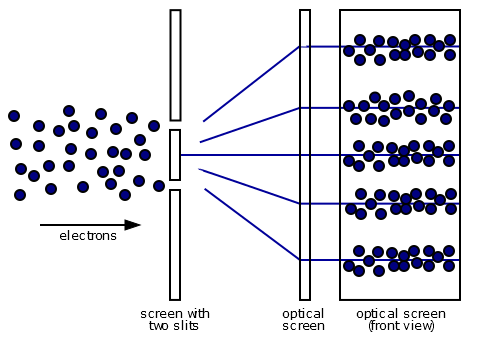
\includegraphics[width=.45\textwidth]{Chapter02/Two-Slit_Experiment_Electrons.png}}  ;
     \node[below right] at (interfere.south west) {(A) Particles exhibiting interference.};
     \node[inner sep=0pt] (noninterfere) at (7,0)
     {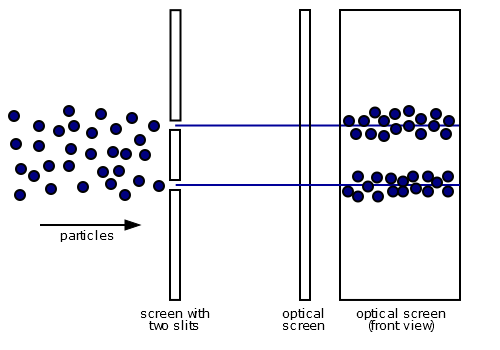
\includegraphics[width=.45\textwidth]{Chapter02/Two-Slit_Experiment_Particles.png}};
     \node[below right] at (noninterfere.south west) {(B) Particles not exhibiting interference.};
    \end{tikzpicture}
    \DIFdelbeginFL %DIFDELCMD < \vspace*{10px}
%DIFDELCMD <     %%%
\DIFdelendFL \caption[Double-Slit Experiment]{The Double-Slit Experiment. Particles are incident on a double slit. In diagram (A), the particles are exhibiting an interference pattern, whereas in diagram (B), the particles are not exhibiting an interference pattern. Whether or not there is interference will depend on factors such as the size of the particles and whether it can be ascertained which slit the particle went through. The larger the particles are, or the more information available as to which slit the particle went through, the less likely the particles will exhibit interference.\protect\footnotemark}
    \label{DoubleSlit}
    \end{figure}
    As figure \ref{DoubleSlit} indicates,\DIFaddbegin \footnotetext{\DIFadd{Diagrams (A) and (B) are by inductiveload, and are Public domain, via Wikimedia Commons. Sources: https://commons.wikimedia.org/wiki/File:Two-Slit\_Experiment\_Electrons.svg and https://commons.wikimedia.org/wiki/File:Two-Slit\_Experiment\_Particles.svg.}} \DIFaddend when a beam of particles is incident on a double slit, the particles that are detected on the detection screen are distributed according to a distribution pattern which either exhibits quantum interference as shown on the left in the figure, or does not exhibit such interference as shown on the right. Small particles like electrons and photons will tend to exhibit quantum interference, whereas mesoscopic particles  will not typically exhibit \DIFaddbegin {\interfootnotelinepenalty\DIFadd{=10000 }\DIFaddend quantum interference.\footnote{There are exceptions to this rule. \DIFdelbegin \DIFdel{For example, }\DIFdelend \DIFaddbegin \DIFadd{E.g. }\DIFaddend a \textbf{Superconducting Quantum Interference Devices (SQUID)}\index{Superconducting Quantum Interference Devices (SQUID)}  can demonstrate quantum interference even at macroscopic scales where a large superconductor can enter into a superposition of two states with the current flowing in opposite directions in each state. See \cite[ch. 6]{Schlosshauer}.}  \DIFaddbegin }
    \DIFaddend 

    To explain what is going on, we suppose that when just the top slit is open, the normalized state of the particle is $\ket*{\psi_1}$,\label{psi_slit} whereas if just the bottom slit is open, we suppose that the normalized state of the particle is $\ket*{\psi_2}$, and when both slits are open, we suppose that the state of the particle will be $\frac{1}{\sqrt{2}}(\ket*{\psi_1}+\ket*{\psi_2})$. 
     Now let the variable $x$ describe the position on the detection screen. For instance, we might take $x=0$ to be the center of the detection screen, and take  positive values of $x$ as corresponding to positions on the upper part of the screen, and negative values of $x$ as corresponding to positions on the lower part of the screen, but the precise convention we adopt won't matter. \DIFdelbegin \footnotetext{\DIFdel{Diagrams (A) and (B) are by inductiveload, and are Public domain, via Wikimedia Commons. Sources: https://commons.wikimedia.org/wiki/File:Two-Slit\_Experiment\_Electrons.svg and https://commons.wikimedia.org/wiki/File:Two-Slit\_Experiment\_Particles.svg.}} %DIFAUXCMD
\DIFdelend Then we define the  $\ket*{x}$-state\DIFdelbegin %DIFDELCMD < \footnotemark%%%
\DIFdel{\;}\DIFdelend \DIFaddbegin \footnote{\label{ketx}\DIFadd{$\ket*{x}$ is not really a state in the proper sense. With the states we've seen so far, when $\ket*{\phi}$ and $\ket*{\psi}$ have been normalized, then $\abs{\ip{\phi}{\psi}}^2$ will be a conditional probability, and hence at most $1$. However, $\ket*{x}$ %DIF > 
     }\nomenclature{$\ket*{x}$}{A non-normalizable position state \nomrefpage}%DIF > 
     \DIFadd{cannot be normalized. This is because the bracket  $\ip{x}{y}$ is defined to be $\ip{x}{y}=\var(x-y)$ where $\var(x)$ is the %DIF > 
     }\nomenclature{$\var(x)$}{The Dirac delta function, \nomrefpage}%DIF > 
          \emph{\DIFadd{Dirac delta}}\index{Dirac delta} \DIFadd{function such that }\begin{equation} 
         \DIFadd{\var(x)=
         \begin{cases} \infty & \text{if $x=0$,} \\
         0 & \text{if $x\neq 0$},
         \end{cases}
         }\end{equation} \DIFadd{and has the property that 
         $\int \dd x \var(x) f(x) = f(0)$ for any continuous function $f(x)$. The theory of distributions allows one to deal rigorously with Dirac delta functions. E.g. see \mbox{%DIFAUXCMD
\cite[ch. 6]{Rudin}}\hskip0pt%DIFAUXCMD
.  
         }} \DIFaddend as the physical state describing the particle to be exactly located at position $x$ on the screen. Note that the state $\ket*{x}$ is indexed by a continuous parameter, $x$. This is in contrast to the basis of states $\ket*{s_i}$ which we have been considering up until now which are indexed by discrete values of $i$ such as $i=1,\,2,\ldots.$ Because of this difference, we need to use calculus to deal with $\ket*{x}$-states in a rigorous manner, but such details will not concern us here. In reality, because of the Heisenberg uncertainty principle, a particle is never in just one $\ket*{x}$-state, but rather the particle will be in a superposition of many $\ket*{x}$-states, which may or may not be concentrated around a particular location, $x_0$ say. The more concentrated these  $\ket*{x}$-states of this superposition are concentrated around a particular location $x_0$, the more the particle will have the particle-like characteristic of being localized in one place. But if the  $\ket*{x}$-states of this superposition are more spread out, the particle will have more wave-like characteristics. So when physicists speak of particles, often they are not thinking of physical entities that are very localized in position, as non-physicists would think. Nevertheless, at the moment the particle is detected on the detection screen, it does seem to be highly localized.
    \DIFdelbegin \footnotetext{%DIFDELCMD < \label{ketx}%%%
\DIFdel{$\ket*{x}$ is not really a state in the proper sense. With the states we've seen so far, when $\ket*{\phi}$ and $\ket*{\psi}$ have been normalized, then $\abs{\ip{\phi}{\psi}}^2$ will be a conditional probability, and hence at most $1$. However, $\ket*{x}$ %DIF < 
}%DIFDELCMD < \nomenclature{$\ket*{x}$}{A non-normalizable position state \nomrefpage}%%%
%DIF < 
\DIFdel{cannot be normalized. This is because the bracket  $\ip{x}{y}$ is defined to be $\ip{x}{y}=\var(x-y)$ where $\var(x)$ is the %DIF < 
}%DIFDELCMD < \nomenclature{$\var(x)$}{The Dirac delta function, \nomrefpage}%%%
%DIF < 
     \emph{\DIFdel{Dirac delta}}%DIFAUXCMD
%DIFDELCMD < \index{Dirac delta} %%%
\DIFdel{function such that }\begin{displaymath} 
    \DIFdel{\var(x)=
    \begin{cases} \infty & \text{if $x=0$,} \\
    0 & \text{if $x\neq 0$},
    \end{cases}
    }\end{displaymath}%DIFAUXCMD
%DIFDELCMD <  %%%
\DIFdel{and has the property that 
    $\int \dd x \var(x) f(x) = f(0)$ for any continuous function $f(x)$. The theory of distributions allows one to deal rigorously with Dirac delta functions. E.g. see \mbox{%DIFAUXCMD
\cite[ch. 6]{Rudin}}\hskip0pt%DIFAUXCMD
.  
    }}
    %DIFAUXCMD
\DIFdelend 

     Given a state $\ket*{\psi}$ for a so-called particle, we define the function $\psi(x)=\ip{x}{\psi}$.  %
\nomenclature{$\psi(x)$}{The wave function corresponding to the state $\ket*{\psi}$ given by the formula $\psi(x)=\ip{x}{\psi}$,  \nomrefpage}%
     Because of the continuous nature of the variable $x$ (in contrast to the discrete nature of $i$ in a basis $\{\ket*{s_i}:i\}$), the function 
     \begin{equation}\label{rhodensity}
     \rho(x)=\abs{\psi(x)}^2
     \end{equation}  
     determines a probability density for a range of outcomes rather than a probability for a specific outcome. Here, we do not need to go into the details of probability densities,\footnote{But if you are interested, a probability density $\rho(x)$ for a random variable $X$ that has real values is a function such that $\rho(x)\geq 0\, \,\forall x\in\mathbb{R}$, and that $\int_\mathbb{R} \rho(x) \dd x =1$ and the probability that $X$ has a value in the subset $U\subset\mathbb{R}$ is $\int_U \rho(x) \dd x $. } but roughly speaking, the greater the value of $\rho(x)$, the greater will be the relative probability of detecting the particle in the vicinity of location $x$. Thus, if $\rho(x')=0$ for all $x'$ in the vicinity of $x$, then the particle would not be detected in the vicinity of location $x$.   

     Now if  $\ket*{\psi}=\frac{1}{\sqrt{2}}(\ket*{\psi_1}+\ket*{\psi_2})$, then 
     $\psi(x)=\frac{1}{\sqrt{2}}(\psi_1(x)+\psi_2(x)).$ Therefore, the corresponding probability density will be\DIFdelbegin \begin{displaymath}\DIFdel{\abs{\psi(x)}^2=\frac{1}{2}(\abs{\psi_1(x)}^2+\abs{\psi_2(x)}^2+2\Re(\overline{\psi_1(x)}\psi_2(x)).\protect\footnotemark
    }\end{displaymath}%DIFAUXCMD
%DIFDELCMD <     %%%
\DIFdelend \DIFaddbegin \phantom{\footnotemark}\DIFaddend \footnotetext{Here $\Re$ %
 \nomenclature{$\Re(z)$}{The real part of a complex number $z$,  \nomrefpage}%
     means the real part of a complex number. Thus, if the complex number $z=\alpha+i\beta$ for real numbers $\alpha$ and $\beta$, then $\Re(z)=\alpha$. To see why the above equation holds, we recall that $\abs{z}^2=z\overline{z}$ and that $\Re(z)=\frac{1}{2}(z+\overline{z})$. Therefore, if $z=\frac{1}{\sqrt{2}}(v+w)$ for complex number $v$ and $w$, then $\abs{z }^2 =\frac{1}{\sqrt{2}}(v+w)\frac{1}{\sqrt{2}}\overline{(v+w)}= \frac{1}{2}(v+w)\overline{(v+w)}=\frac{1}{2}(v\overline{v}+w\overline{w}+w\overline{v}+v\overline{w})=\frac{1}{2}(\abs{v}^2+\abs{w}^2+w\overline{v}+\overline{w\overline{v}})=\frac{1}{2}(\abs{v}^2+\abs{w}^2+2\Re(\overline{v}w))$.}
\DIFaddbegin 

     \vspace{-37pt}%DIF > yyyyyyyyyyyyyyyyy
     \begin{equation*}\DIFadd{\abs{\psi(x)}^2=\frac{1}{2}(\abs{\psi_1(x)}^2+\abs{\psi_2(x)}^2+2\Re(\overline{\psi_1(x)}\psi_2(x)).\protect\footnotemark[\thefootnote]
    \vspace{-7.96pt} 
    }\end{equation*}\DIFaddend Now when the detection screen is far away from the double slits, we will have $\abs{\psi_1(x)}^2\approx \abs{\psi_2(x)}^2$ for $x$ near the center point on the screen. However, depending on slight changes in the value of $x$ from the center point on the screen, sometimes $\psi_1(x)$ and $\psi_2(x)$ will be in phase so that  $\psi_1(x)\approx\psi_2(x)$, in which case $\abs{\psi(x)}^2\approx 2\abs{\psi_1(x)}^2$. But sometimes $\psi_1(x)$ and $\psi_2(x)$ will be  out of phase so that $\psi_1(x)\approx-\psi_2(x),$ in which case $\abs{\psi(x)}^2\approx 0$. Hence, we get the interference pattern as shown in figure \ref{DoubleSlit} (A).

    Now in order to consider how decoherence affects interference, we let 
\DIFdelbegin \begin{displaymath}\DIFdel{\ket*{\Psi(t)}=\frac{1}{\sqrt{2}}(\ket*{\psi_1}\ket*{E_1(t)}+\ket*{\psi_2}\ket*{E_2(t)})}\end{displaymath}%DIFAUXCMD
\DIFdelend \DIFaddbegin 

    
    \vspace{-37pt}%DIF > yyyyyyyyyyyyyyyyy
    \begin{equation*}
\DIFadd{\ket*{\Psi(t)}=\frac{1}{\sqrt{2}}(\ket*{\psi_1}\ket*{E_1(t)}+\ket*{\psi_2}\ket*{E_2(t)})
\vspace{-7.96pt} 
}\end{equation*}\DIFaddend  be the state of the composite system $\mathcal{U}=\mathcal{S}+\mathcal{E}$ where $\mathcal{S}$ is a particle that has gone through the double slit and will be detected on the detection screen, and $\mathcal{E}$ is the local environment of the experimental set up. The expression for $\ket*{\Psi(t)}$ indicates that we are assuming  $\mathcal{S}$ doesn't become entangled with $\mathcal{E}$ when $\mathcal{S}$ is in the state $\ket*{\psi_1}$ or $\ket*{\psi_2}$. Corresponding to $\ket*{\Psi(t)}$, we can define the density matrix  $\hat{\rho}(t)=\dyad{\Psi(t)}.$  We can also define the observable\footnote{Note that we only call $\dyad{x}_\mathcal{S}$ an observable in an analogical sense since it is not a compact Hermitian operator acting on the Hilbert space of states $H_\mathcal{S}$. If we were being more rigorous, we would need to consider a Hermitian operator of the form $\int \sigma(x)\dyad{x}_\mathcal{S}\dd x$ for an appropriate test function $\sigma(x)$. } $\dyad{x}_\mathcal{S}$ for the system $\mathcal{S}$ so that $\dyad{x}_\mathcal{S}\ket*{\psi}_\mathcal{S}=\psi(x)\ket*{x}_\mathcal{S}.$ As we saw in equation (\ref{extension}) on page \pageref{extension}, we can naturally extend the action of $\dyad{x}_\mathcal{S}$ to $H_\mathcal{U}$.\footnote{Strictly speaking, it is not $\dyad{x}_\mathcal{S}$ that is extended to act on $H_\mathcal{U}$, but rather a Hermitian operator of the form $\int \sigma(x)\dyad{x}_\mathcal{S}\dd x$ for an appropriate test function $\sigma(x)$ that is extended to $H_\mathcal{U}$. For a state $\ket*{\xi}_\mathcal{U}=\ket*{\psi}_\mathcal{S}\ket*{E}_\mathcal{E}$, the action of $\dyad{x}_\mathcal{U}$ on $\ket*{\xi}_\mathcal{U}$ gives the `state' $\dyad{x}_\mathcal{U}\ket*{\xi}_\mathcal{U}\myeq\psi(x)\ket*{x}_\mathcal{S}\ket*{E}_\mathcal{E}$, but since this is not normalizable, we have to `smear' it by integrating it with respect to the test function $\sigma(x)$.}  
    This allows us to define 
\DIFdelbegin \begin{displaymath}\DIFdel{\rho_\mathcal{U}(x, t)\myeq\Tr_\mathcal{U}(\hat{\rho}(t)_\mathcal{U}\dyad{x}_\mathcal{U}).}\end{displaymath}%DIFAUXCMD
\DIFdelend \DIFaddbegin 


    \vspace{-37pt}%DIF > yyyyyyyyyyyyyyy
    \begin{equation*}
\DIFadd{\rho_\mathcal{U}(x, t)\myeq\Tr_\mathcal{U}(\hat{\rho}(t)_\mathcal{U}\dyad{x}_\mathcal{U}).
\vspace{-7.96pt}
}\end{equation*}\DIFaddend 
     In the specific case when $\mathcal{S}$ and $\mathcal{E}$ are not entangled so that $\hat{\rho}_\mathcal{U}(t)=\dyad{\xi(t)}_\mathcal{U}$ with $\ket*{\xi(t)}_\mathcal{U}=\ket*{\psi}_\mathcal{S}\ket*{E(t)}_\mathcal{E}$ for normalized states $\ket*{\psi}_\mathcal{S}$ and $\ket*{E(t)}_\mathcal{E}$, we have $\rho_\mathcal{U}(x, t) =\abs{\psi(x)}^2$ which is equal to the probability density function $\rho(x)$ we saw in equation (\ref{rhodensity}).\footnote{To see this, note that we can ignore $\mathcal{E}$ in calculating $\ev*{\dyad{x}_\mathcal{U}}_\xi$ since when $\mathcal{S}$ and $\mathcal{E}$ are not entangled, $\ev*{\dyad{x}_\mathcal{U}}_\xi = \ev*{\dyad{x}_\mathcal{S}}_\psi$ as explained in footnote \footreference{untangledobservable}. We can therefore just consider $\mathcal{S}$ and drop the subscripts.
    Furthermore, as we saw in equation (\ref{expdensity}), $\ev*{\hat{O}}_\psi=\Tr(\hat{\rho}\hat{O})$ where $\hat{\rho}=\dyad{\psi}$. 
    We can thus take an orthonormal basis $\{\ket*{\psi_1},\ket*{\psi_2},\ldots\}$ of $H_\mathcal{S}$ with $\ket*{\psi_1}=\ket*{\psi}$. 
    Then $\rho(x)=\Tr(\hat{\rho}\dyad{x})=\Tr(\dyad{\psi}\dyad{x})=\sum_i\ip{\psi_i}{\psi}\ip{\psi}{x}\ip{x}{\psi_i}=\ip{\psi_1}{\psi}\ip{\psi}{x}\ip{x}{\psi_1} =\ip{\psi}{x}\ip{x}{\psi}=\overline{\ip{x}{\psi}}\ip{x}{\psi}=\abs{\ip{x}{\psi}}^2=\abs{\psi(x)}^2.$} 
    However, if $\ket*{E_1(t)}_\mathcal{E}$ is not proportional to $\ket*{E_2(t)}_\mathcal{E}$, then $\ket*{\Psi(t)}$ will be an entangled state of $\mathcal{S}$ and $\mathcal{E}$. But whether or not $\mathcal{S}$ and $\mathcal{E}$ are entangled, we can still use equation (\ref{reduced}) to calculate the partial trace:
    \DIFdelbegin \begin{displaymath}\DIFdel{\hat{\rho}_\mathcal{S}(t)=\frac{1}{2}(\dyad{\psi_1}_\mathcal{S}+\dyad{\psi_2}_\mathcal{S}+\ip{E_2(t)}{E_1(t)}_\mathcal{E} \dyad{\psi_1}{\psi_2}_\mathcal{S}+\ip{E_1(t)}{E_2(t)}_\mathcal{E} \dyad{\psi_2}{\psi_1}_\mathcal{S}).}\end{displaymath}%DIFAUXCMD
\DIFdelend \DIFaddbegin 


    \vspace{-37pt}%DIF > yyyyyyyyyyyyyyy
    \begin{equation*}
\DIFadd{\hat{\rho}_\mathcal{S}(t)=\frac{1}{2}(\dyad{\psi_1}_\mathcal{S}+\dyad{\psi_2}_\mathcal{S}+\ip{E_2(t)}{E_1(t)}_\mathcal{E} \dyad{\psi_1}{\psi_2}_\mathcal{S}+\ip{E_1(t)}{E_2(t)}_\mathcal{E} \dyad{\psi_2}{\psi_1}_\mathcal{S}).
\vspace{-7.96pt} 
}\end{equation*}\DIFaddend 
By equations (\ref{expdensity}) and (\ref{reducedev}), we therefore have
\begin{equation}\rho_\mathcal{U}(x, t)=\frac{1}{2}\Big(\abs{\psi_1(x)}^2+\abs{\psi_2(x)}^2+2\Re\big(\ip{E_2(t)}{E_1(t)}_\mathcal{E}\overline{\psi_2(x)}\psi_1(x)\big)\Big).\protect\footnotemark
\end{equation}
Thus, \footnotetext{The calculation is as follows:
\DIFdelbegin \begin{displaymath}
    \begin{split}\DIFdel{\rho_\mathcal{U}(x, t)}&\DIFdel{=\Tr_\mathcal{U}(\hat{\rho}(t)_\mathcal{U}\dyad{x}_\mathcal{U})=
    \ev*{\dyad{x}_\mathcal{U}}_{\rho(t)}=\Tr_\mathcal{S}(\hat{\rho}_\mathcal{S}(t)\dyad{x}_\mathcal{S})}\\
    &\DIFdel{=\Tr_\mathcal{S}\Big(\frac{1}{2}(\dyad{\psi_1}_\mathcal{S}+\dyad{\psi_2}_\mathcal{S}}\\
    &\DIFdel{\qquad+\ip{E_2(t)}{E_1(t)}_\mathcal{E} \dyad{\psi_1}{\psi_2}_\mathcal{S}+\ip{E_1(t)}{E_2(t)}_\mathcal{E} \dyad{\psi_2}{\psi_1}_\mathcal{S})\dyad{x}_\mathcal{S}\Big)}\\
    &\DIFdel{=\Tr_\mathcal{S}\Big(\frac{1}{2}(\ip{\psi_1}{x}_\mathcal{S}\dyad{\psi_1}{x}_\mathcal{S}+\ip{\psi_2}{x}_\mathcal{S}\dyad{\psi_2}{x}_\mathcal{S}}\\&\DIFdel{\qquad+\ip{E_2(t)}{E_1(t)}_\mathcal{E}\ip{\psi_2}{x}_\mathcal{S}\dyad{\psi_1}{x}_\mathcal{S}+\ip{E_1(t)}{E_2(t)}_\mathcal{E} \ip{\psi_1}{x}_\mathcal{S}\dyad{\psi_2}{x}_\mathcal{S})\Big)
    }\\
    &\DIFdel{=\frac{1}{2}\Big(\ip{\psi_1}{x}_\mathcal{S}\ip{x}{\psi_1}_\mathcal{S}+\ip{\psi_2}{x}_\mathcal{S}\ip{x}{\psi_2}_\mathcal{S}}\\&\DIFdel{\qquad+\ip{E_2(t)}{E_1(t)}_\mathcal{E}\ip{\psi_2}{x}_\mathcal{S}\ip{x}{\psi_1}_\mathcal{S}+\ip{E_1(t)}{E_2(t)}_\mathcal{E}\ip{\psi_1}{x}_\mathcal{S}\ip{x}{\psi_2}_\mathcal{S}\Big)}\\
    &\DIFdel{=\frac{1}{2}\Big(\overline{\ip{x}{\psi_1}_\mathcal{S}}\ip{x}{\psi_1}_\mathcal{S}+\overline{\ip{x}{\psi_2}_\mathcal{S}}\ip{x}{\psi_2}_\mathcal{S}}\\&\DIFdel{\qquad+\ip{E_2(t)}{E_1(t)}_\mathcal{E}\overline{\ip{x}{\psi_2}_\mathcal{S}}\ip{x}{\psi_1}_\mathcal{S}+\overline{\ip{E_2(t)}{E_1(t)}_\mathcal{E}\overline{\ip{x}{\psi_2}_\mathcal{S}}\ip{x}{\psi_1}_\mathcal{S}}\Big)
    }\\
    &\DIFdel{=\frac{1}{2}\Big(\abs{\psi_1(x)}^2+\abs{\psi_2(x)}^2+2\Re\big(\ip{E_2(t)}{E_1(t)}_\mathcal{E}\overline{\psi_2(x)}\psi_1(x)\big)\Big).
    }\end{split}
    \DIFdel{}\end{displaymath}%DIFAUXCMD
\DIFdelend \DIFaddbegin \newline  \noindent \DIFadd{$\rho_\mathcal{U}(x, t)=\Tr_\mathcal{U}(\hat{\rho}(t)_\mathcal{U}\dyad{x}_\mathcal{U})=
\ev*{\dyad{x}_\mathcal{U}}_{\rho(t)}=\Tr_\mathcal{S}(\hat{\rho}_\mathcal{S}(t)\dyad{x}_\mathcal{S})$ 
}\newline
\DIFadd{$=\Tr_\mathcal{S}\Big(\frac{1}{2}(\dyad{\psi_1}_\mathcal{S}+\dyad{\psi_2}_\mathcal{S}
+\ip{E_2(t)}{E_1(t)}_\mathcal{E} \dyad{\psi_1}{\psi_2}_\mathcal{S}+\ip{E_1(t)}{E_2(t)}_\mathcal{E} \dyad{\psi_2}{\psi_1}_\mathcal{S})\dyad{x}_\mathcal{S}\Big)$
}\newline\DIFadd{$= \Tr_\mathcal{S}\Big(\frac{1}{2}(\ip{\psi_1}{x}_\mathcal{S}\dyad{\psi_1}{x}_\mathcal{S}+\ip{\psi_2}{x}_\mathcal{S}\dyad{\psi_2}{x}_\mathcal{S}+\ip{E_2(t)}{E_1(t)}_\mathcal{E}\ip{\psi_2}{x}_\mathcal{S}\dyad{\psi_1}{x}_\mathcal{S}$
}

\DIFadd{$+\ip{E_1(t)}{E_2(t)}_\mathcal{E} \ip{\psi_1}{x}_\mathcal{S}\dyad{\psi_2}{x}_\mathcal{S})\Big)$
}\newline\DIFadd{$=\frac{1}{2}\Big(\ip{\psi_1}{x}_\mathcal{S}\ip{x}{\psi_1}_\mathcal{S}+\ip{\psi_2}{x}_\mathcal{S}\ip{x}{\psi_2}_\mathcal{S}+\ip{E_2(t)}{E_1(t)}_\mathcal{E}\ip{\psi_2}{x}_\mathcal{S}\ip{x}{\psi_1}_\mathcal{S}$
}

\DIFadd{$+\ip{E_1(t)}{E_2(t)}_\mathcal{E}\ip{\psi_1}{x}_\mathcal{S}\ip{x}{\psi_2}_\mathcal{S}\Big)$
}\newline\DIFadd{$=\frac{1}{2}\Big(\overline{\ip{x}{\psi_1}_\mathcal{S}}\ip{x}{\psi_1}_\mathcal{S}+\overline{\ip{x}{\psi_2}_\mathcal{S}}\ip{x}{\psi_2}_\mathcal{S}+\ip{E_2(t)}{E_1(t)}_\mathcal{E}\overline{\ip{x}{\psi_2}_\mathcal{S}}\ip{x}{\psi_1}_\mathcal{S}$
}

\DIFadd{$+\overline{\ip{E_2(t)}{E_1(t)}_\mathcal{E}\overline{\ip{x}{\psi_2}_\mathcal{S}}\ip{x}{\psi_1}_\mathcal{S}}\Big)$    
}\newline\DIFadd{$=\frac{1}{2}\Big(\abs{\psi_1(x)}^2+\abs{\psi_2(x)}^2+2\Re\big(\ip{E_2(t)}{E_1(t)}_\mathcal{E}\overline{\psi_2(x)}\psi_1(x)\big)\Big).$}\DIFaddend }if $\ip{E_1(t)}{E_2(t)}_\mathcal{E}\approx 0$ then 
$\rho_\mathcal{U}(x, t)\approx\frac{1}{2}\Big(\abs{\psi_1(x)}^2+\abs{\psi_2(x)}^2\Big)$
and so we would observe a distribution pattern not exhibiting interference  as shown in figure \ref{DoubleSlit} (B). On the other hand, if  $\ip{E_1(t)}{E_2(t)}_\mathcal{E}\not\approx 0$ we would get a distribution pattern exhibiting interference as shown in figure \ref{DoubleSlit} (B). Therefore, since it is often possible to determine the asymptotic behavior of $\ip{E_1(t)}{E_2(t)}_\mathcal{E}$,\footnote{i.e. whether or not $\ip{E_1(t)}{E_2(t)}_\mathcal{E}\rightarrow 0$ as $t\rightarrow\infty$ and how fast this convergence might take place. } decoherence theory gives us a means of determining whether or not quantum interference will be exhibited. 

    
   
% flatex input end: [Chapter02/Interference.tex]

%\usepackage[inline]{showlabels}
 % flatex input: [Chapter02/ProblemOfOutcomes.tex]

    \section{The Problem of Outcomes}\label{probOutcomes}
    In the last two sections we have seen how decoherence theory solves the preferred basis problem and the problem of the nonobservability of interference. However, there is a third fundamental problem in quantum physics which decoherence theory is unable to solve. This is the problem of outcomes. As discussed in subsection \ref{vonNeumannMeasurement}, in the von Neumann measurement scheme, it is supposed that for the measurement of a physical system $\mathcal{S}$ to take place, it must interact with a measuring device $\mathcal{A}$ which together satisfy the conditions \ref{vonNeumannMeasurement1}. and \ref{vonNeumannMeasurement2}. on page \pageref{vonNeumannMeasurement1}. If $\mathcal{S}$ is initially in a superposition of states $\ket*{\psi}=\sum_i c_i\ket*{s_i}$ then for $\mathcal{A}$ to measure $\mathcal{S}$, it is necessary for the combined system $\mathcal{S}+\mathcal{A}$ to enter into a superposition
    \begin{equation}\label{vNevolution}
    \ket*{\psi}\ket*{a_r(t_0)}\xrightarrow{\text{time evolution}}\sum_i c_i\ket*{s_i}\ket*{a_i(t)}.
    \end{equation}
    However, although the evolution described in (\ref{vNevolution}) must take place if $\mathcal{A}$ is to measure $\mathcal{S}$, it is not sufficient. When one takes the partial trace of $\dyad{\psi}$ over $\mathcal{A}$, then according to (\ref{reduced}),
    \begin{equation}\label{vNevolution2}
    \tr_\mathcal{A}(\dyad{\psi})\xrightarrow{\text{time evolution}}\sum_i \abs{c_i}^2\dyad{s_i}.
    \end{equation} 
    But as noted on page \pageref{Espagnat}, we cannot give an ignorance interpretation to $\sum_i \abs{c_i}^2\dyad{s_i}$ for as d'Espagnat puts it, this is an improper mixture. When considered together, the system $\mathcal{S}$ and the apparatus $\mathcal{A}$ remain in the superposition described by (\ref{vNevolution}), and so none of the measurement outcomes from the set of possible outcomes $\{\ket*{s_i}:i\}$ have actually occurred. The problem of explaining how the composite system   $\mathcal{S}+\mathcal{A}$       goes from being in the state $\sum_i c_i\ket*{s_i}\ket*{a_i(t)}$ to a state $\ket*{s_i}\ket*{a_i(t)}$ is known as the \textbf{problem of outcomes}\index{problem of outcomes}.\label{proboutcomes}  
% flatex input end: [Chapter02/ProblemOfOutcomes.tex]

%\usepackage[inline]{showlabels}
% flatex input: [Chapter02/Many-WorldsInterpretation.tex]

    \section{The Many-Worlds Interpretation}\label{manyworldsinterpretation1}
    Not everyone is convinced that the problem of outcomes is a genuine problem. In particular, physicists such as Everett, De Witt, Deutsch, Zeh, and Zurek\footnote{For a short history of the development of the many-worlds interpretation, see \cite[336--337]{Schlosshauer}. The central idea underlying the many-worlds was first described in \cite{EverettHugh1957RSFo}. Everett's idea and the idea of branching worlds was popularized in \cite{DeWittBryceS.1970Qmar} and \cite{DEUTSCHD1985Qtaa}. Zeh and Zurek used Everett's ideas in their development of decoherence theory, e.g. see \cite{ZehH.D.1993Tanq} and \cite{ZurekWojciechH.1998Deat}.} who endorse the many-worlds interpretation of quantum physics effectively argue that there are no outcomes in the traditional sense. In this section, we give an account of the many-worlds interpretation of quantum physics and why physicists find it attractive. To this end, let us consider a physical universe $\mathcal{U}=\mathcal{S}+\mathcal{A}+\mathcal{P}_A+\mathcal{P}_B+\mathcal{E}$ consisting of subsystems $\mathcal{S}, \mathcal{A}, \mathcal{P}_A,\mathcal{P}_B$  %
\nomenclature{$\mathcal{P}_A,\mathcal{P}_B$}{The physical systems corresponding to two scientists, Alice and Bob respectively, \nomrefpage}%
    and $\mathcal{E}$. $\mathcal{S}$ is the physical system under investigation; $\mathcal{A}$ is some measuring apparatus that interacts with $\mathcal{S}$; $\mathcal{P}_A$ and $\mathcal{P}_B$ are the physical systems corresponding to two scientists, Alice and Bob who observed the apparatus $\mathcal{A}$; and $\mathcal{E}$ is the remainder of the physical universe $\mathcal{U}$.  For convenience, we define the composite subsystem $\mathcal{V}=\mathcal{S}+\mathcal{A}+\mathcal{P}_A+\mathcal{P}_B$ %
\nomenclature{$\mathcal{V}$}{The composite subsystem $\mathcal{S}+\mathcal{A}+\mathcal{P}_A+\mathcal{P}_B$ so that $\mathcal{U}=\mathcal{V}+\mathcal{E}$, \nomrefpage}%
    so that $\mathcal{U}=\mathcal{V}+\mathcal{E}$. As above on page \pageref{pointer}, we  assume that there is an orthonormal basis $\{\ket*{s_i}:i\}$ of $H_\mathcal{S}$ which we again refer to as pointer states, but now we assume that there are ready states $\ket*{a_r(t)}\in H_\mathcal{A},\,\ket*{p_{r, A}(t)}\in H_{\mathcal{P}_A},\,\ket*{p_{r, B}(t)}\in H_{\mathcal{P}_B},$ and  %
\nomenclature{$\ket*{p_{r, A}(t)}, \ket*{p_{r, B}(t)}$}{Ready states of Alice and Bob before they observe a measurement outcome, \nomrefpage}%
    $\ket*{E_r(t)}\in H_\mathcal{E}$ and %
    \nomenclature{$\ket*{E_r(t)}$}{Ready states of the environment $\mathcal{E}$, \nomrefpage}%
    that for each $i$, there are normalized states $\ket*{a_i(t)}\in H_\mathcal{A},\,\ket*{p_{i, A}(t)}\in H_{\mathcal{P}_A},\,\ket*{p_{i, B}(t)}\in H_{\mathcal{P}_B},$ and $\ket*{E_i(t)}\in H_\mathcal{E}$ such 
     %
    \nomenclature{$\ket*{E_i(t)}$}{State of the environment $\mathcal{E}$ corresponding to the pointer state $\ket*{s_i}$, \nomrefpage}%
    that 
      %
\nomenclature{$\ket*{p_{i, A}(t)}, \ket*{p_{i, B}(t)}$}{The states of Alice and Bob after they have observed the apparatus to be in the state $\ket*{a_i(t)}$, \nomrefpage}%
\begin{enumerate}[noitemsep, nosep, topsep=0pt]
  \item for any $t\geq 0$ we have the evolution of the states 
  \DIFaddbegin \vspace{-15 pt}
  \DIFaddend \begin{align*}\ket*{s_i}\ket*{a_r(t)}\ket*{p_{r, A}(t)}&\ket*{p_{r, B}(t)}\ket*{E_r(t)}\\ &\xrightarrow{\text{time evolution}}\ket*{s_i}\ket*{a_i(t)}\ket*{p_{i, A}(t)}\ket*{p_{i, B}(t)}\ket*{E_i(t)},\end{align*}
  \DIFaddbegin \vspace{-80 pt}\newline
  \DIFaddend \item there exists $\delta>0$ such that if $t>t_0+\delta$, then for $i\neq j$, $\ip{a_i(t)}{a_j(t)}\approx 0$, $\ip{p_{i, A}(t)}{p_{j, A}(t)}\approx 0$, $\ip{p_{i, B}(t)}{p_{j, B}(t)}\approx 0$ and $\ip{E_i(t)}{E_j(t)}\approx 0$.\footnote{Again, recall footnote \footreference{approx}.}
  \end{enumerate}
  We also suppose that the $\ket*{p_{i,A}(t)}$-state would describe actions of Alice consistent with her observing the apparatus being in the $\ket*{a_i(t)}$-state, for example, her writing down in her log book that the apparatus is in the $\ket*{a_i(t)}$-state or telling her colleague that this is the case. Likewise, we assume the $\ket*{p_{i,B}(t)}$-state is consistent with Bob also observing the apparatus to be in the $\ket*{a_i(t)}$-state.

  Now suppose the initial (normalized) state of $\mathcal{S}$ is $\ket*{\psi}=\sum_i c_i\ket*{s_i}$, so that the state for the composite system $\mathcal{U}=\mathcal{V}+\mathcal{E}$ is $\ket*{\Psi(t)}=\sum_i c_i \ket*{\xi_i(t)}\ket*{E_i(t)}\in H_{\mathcal{U}}$ where $\ket*{\xi_i(t)}=\ket*{s_i}\ket*{a_i(t)}\ket*{p_{i,A}(t)}\ket*{p_{i,B}(t)}\in H_{\mathcal{V}}$. %
  \nomenclature{$\ket*{\xi_i(t)}$}{The state $\ket*{s_i}\ket*{a_i(t)}\ket*{p_{i,A}(t)}\ket*{p_{i,B}(t)}\in H_{\mathcal{V}}$ of $\mathcal{V}=\mathcal{S}+\mathcal{A}+\mathcal{P}_A+\mathcal{P}_B$, \nomrefpage}%
   We also define the corresponding density matrix for the composite system $\hat{\rho}=\dyad{\Psi}$. If we were unable to make any observations on $\mathcal{E}$, then 
   the partial trace
  $\hat{\rho}_{\mathcal{V}}(t)=\Tr_\mathcal{E}(\hat{\rho}(t))$ will contain all the information we need to work out the expectation values for any observables of  $\mathcal{V}.$ So just as with equation (\ref{reduced}), we will have
  \begin{equation} \label{reducedv}
  \begin{split}
    \hat{\rho}_{\mathcal{V}}(t)&=\sum_{i}\abs{c_i}^2\dyad{\xi_i(t)}+\sum_{i\neq j}c_i\overline{c_j}\ip{E_j(t)}{E_i(t)}\dyad{\xi_i(t)}{\xi_j(t)}\\
    &\approx \sum_{i}\abs{c_i}^2\dyad{\xi_i(t)}
    \end{split}\end{equation}
    \DIFaddbegin \newline\phantom{zzzz}\vspace{-60pt}

    \noindent \DIFaddend for $t>t_0+\delta.$ Then the expectation values of any observables on $\mathcal{V}$ will be indistinguishable from the scenario in which $\mathcal{V}$ is actually in one of the $\ket*{\xi_i(t)}$-states \DIFaddbegin {\interfootnotelinepenalty\DIFadd{=10000 }\DIFaddend with probability $\abs{c_i}^2$.\footnote{Again recall the discussion following equation (\ref{rhodiag}) on page \pageref{rhodiag}. There is the question of uniqueness of $\hat{\rho}_{\mathcal{V}}=\sum_{i}\abs{c_i}^2\dyad{\xi_i(t)}$. If all the $\abs{c_i}^2$ are unique, then if we have another decomposition $\hat{\rho}_{\mathcal{S}+\mathcal{A}+\mathcal{P}_A+\mathcal{P}_B}=\sum_{i}\abs{c_i}^2\dyad{\xi_i'(t)}$ it follows that $\ket*{\xi_i(t)}\propto\ket*{\xi_i'(t)}$. But even if some of the $\abs{c_i}^2$ are the same, criteria 1 and 2 above will ensure that states with the same  value of $\abs{c_i}^2$ will be determined up to permutation.} It would\DIFaddbegin } \DIFaddend nevertheless be incorrect for us to conclude on the basis of decoherence theory alone that $\mathcal{V}$ actually was in one of those $\ket*{\xi_i(t)}$-states, since equation (\ref{reducedv}) is based on a subjective distinction between $\mathcal{V}$ and $\mathcal{E}$ in the decomposition $\mathcal{U}=\mathcal{V}+\mathcal{E}.$ Human scientists make this distinction to reflect the fact that they can only perform measurements on $\mathcal{V}$ and can't measure $\mathcal{E}$. But if a super-intelligent being could measure everything in  $\mathcal{U}$, then such a being would not say that $\mathcal{V}$ was in one of the  $\ket*{\xi_i(t)}$-states, but rather that $\mathcal{U}$ was in the state $\ket*{\Psi(t)}$. As we have already discussed on pages \pageref{subtle}--\pageref{subtleend}, the density matrix $ \hat{\rho}_{\mathcal{V}}(t)$ is not a mixed state, but is an improper mixture. 

    Now if we define the observables $\hat{O}_{i,\mathcal{A}}(t)=\dyad{p_{i,A}(t)}$ that %
\nomenclature{$\hat{O}_{i,\mathcal{A}}(t), \hat{O}_{i,\mathcal{B}}(t)$}{The observables $\dyad{p_{i,A}(t)}$ and $\dyad{p_{i,B}(t)}$ respectively,  \nomrefpage}%
    would measure the behavior of Alice, and the observables $\hat{O}_{i,\mathcal{B}}(t)=\dyad{p_{i,B}(t)}$ that would measure the behavior of Bob, then for $t>t_0+\delta$, we see that $\hat{O}_{i,\mathcal{A}}(t)\hat{O}_{j,\mathcal{B}}(t)\ket*{\Psi(t)}\approx 0,$ when $i\neq j$. This means that when we consider $\hat{O}_{i,\mathcal{A}}(t)\hat{O}_{j,\mathcal{B}}(t)$ as an observable acting on $\mathcal{V}$,  the expectation value $\ev*{\hat{O}_{i,\mathcal{A}}(t)\hat{O}_{j,\mathcal{B}}(t)}_{\rho_\mathcal{V}(t)}$ will be approximately zero for $i\neq j$. What this means is that if we consider ourselves as observing Alice and Bob observing the apparatus, then after time $t_0+\delta$, the probability we would see Alice and Bob disagreeing with each other concerning their observations of the apparatus would be approximately 0. 
     On the other hand, since $\hat{O}_{i,\mathcal{A}}(t)\hat{O}_{i,\mathcal{B}}(t)\ket*{\Psi(t)} \approx c_i \ket*{\xi_i(t)}\ket*{E_i(t)}$ for $t>t_0+\delta$, it follows that $\ev*{\hat{O}_{i,\mathcal{A}}(t)\hat{O}_{i,\mathcal{B}}(t)}_{\rho_\mathcal{V}(t)}=\abs{c_i}^2.$ 
     We would thus observe Alice and Bob observing the apparatus to be in the $\ket*{a_i(t)}$-state with probability $\abs{c_i}^2.$ 

     But note that on the assumption that there are no hidden variables, if we did actually make such an observation and this observation corresponded to reality, then the quantum state $\ket*{\Psi(t)}$ would have had to have changed to $\ket*{\xi_i(t)}\ket*{E_i(t)}$, since before our observation when $\ket*{\Psi(t)}$ was a complete description of $\mathcal{U}$, we would say Alice and Bob will measure the $\ket*{a_i(t)}$-state with probability $\abs{c_i}^2$, but when we are actually seeing them measuring the $\ket*{a_i(t)}$-state, we would have to say that now the probability they are measuring the $\ket*{a_i(t)}$-state is $1$, and hence we would say that the system was in the $\ket*{\xi_i(t)}\ket*{E_i(t)}$-state. Whether or not the process of the state going from $\ket*{\Psi(t)}$ to $\ket*{\xi_i(t)}\ket*{E_i(t)}$ was instantaneous or took a non-infinitesimal amount of time, this interpretation would be susceptible to the problems already discussed with the Copenhagen interpretation in section \ref{eprsec}.

    But in the \textbf{many-worlds interpretation}\index{many-worlds interpretation}, rather than assuming that $\ket*{\Psi(t)}=\sum_i c_i \ket*{\xi_i(t)}\ket*{E_i(t)}$ is the complete description of $\mathcal{U}$ that enables us to work the probability of certain outcomes, we simply say that $\ket*{\Psi(t)}$ is a complete description of the state of $\mathcal{U}$, and we drop the assumption that we need to interpret this state as describing probabilities of outcomes. Thus, a many-worlds adherent would say we can understand what the state of $\mathcal{U}$ is on its own terms without the need to appeal to any other extrinsic principle such as measurement. Just as we don't puzzle over how to interpret what a sphere is in terms of an extrinsic principle, we don't need to puzzle over how to interpret the space of states of $\mathcal{U}$. We can think of the mathematical formalism $\ket*{\Psi(t)}=\sum_i c_i \ket*{\xi_i(t)}\ket*{E_i(t)}$ describing the state of $\mathcal{U}$ as being somewhat akin to a point lying on a \DIFaddbegin {\interfootnotelinepenalty\DIFadd{=10000 }\DIFaddend sphere given by the equation $x^2+y^2+z^2=1$.\footnote{On the assumption that $\ket*{\Psi(t)}$ is normalized, we could think of $\ket*{\Psi(t)}$ as specifying a point on the (possibly infinite-dimensional) hypersphere $\{(c_1,c_2\ldots):\sum_i|c_i|^2=1\}.$} Although we might be\DIFaddbegin } \DIFaddend tempted to interpret $\ket*{\Psi(t)}$ as describing the probability of outcomes, we are not obliged to do so,  since these probabilities can instead be understood to be grounded in the symmetries the system possesses rather than in terms of the frequency of how many measurement outcomes are likely to occur. For instance, when we see a coin and judge that it will come up heads with probability $\frac{1}{2}$ and tails with probability $\frac{1}{2}$, we intuit this by looking at the symmetry of the coin rather than tossing the coin millions of times and counting how often it comes up heads and how often it comes up tails. Thus, we might suppose $\ket*{\Psi(t)}$ has analogous symmetries that allow us to determine its $c_i$ coefficients without the need to posit any of the $\ket*{\xi_i(t)}\ket*{E_i(t)}$ measurement outcomes being realized.

    As for the decomposition $\ket*{\Psi(t)}=\sum_i c_i \ket*{\xi_i(t)}\ket*{E_i(t)}$  in terms of the $\ket*{\xi_i(t)}\ket*{E_i(t)}$ basis states, decoherence theory gives us a natural account of why we should choose this basis rather than any other. When $\mathcal{U}$ is in the state $\ket*{\Psi(t_0)}=\Big(\sum_i c_i \ket*{\xi_i(t_0)}\Big)\ket*{E_r(t)}$, we can think of this state as describing one world, $W$ say.  %
\nomenclature{$W$}{A world described by the state $\ket*{\Psi(t_0)}=\Big(\sum_i c_i \ket*{\xi_i(t_0)}\Big)\ket*{E_r(t)}$,  \nomrefpage}%
    But once $t>t_0+\delta$ so that $\ip{E_i(t)}{E_j(t)}\approx 0$ for $i\neq j$, we can think of each $\ket*{\xi_i(t)}\ket*{E_i(t)}$-component as a different world $W_i$.   %
\nomenclature{$W_i$}{A world described by the state $\ket*{\xi_i(t)}\ket*{E_i(t)}$,  \nomrefpage}%
    Thus, for $t>t_0+\delta$, we say the world $W$ has \textbf{branched}\index{branching} into as many-worlds $W_i$ for which the $c_i$ are non-zero. 

    But why should we think that there are literally many worlds? Well, from an ontological point of view, one might very well think that there is really only one world and that this world is described by $\ket*{\Psi(t)};$ it would be a rather weird world since the entanglement between $\mathcal{V}$ and $\mathcal{E}$ would mean there wouldn't be any absolute matters of fact describing $\mathcal{V}$. But it might not be a bad thing to say that the ``many'' in the many-worlds interpretation is really just a figure of speech that we shouldn't take too literally. After all, a common objection to the many-worlds interpretation is that it is ontologically extravagant and that we should appeal to Occam's Razor. But if we just say that there is actually only one world described by $\ket*{\Psi(t)}$ then this ``many''-worlds interpretation is actually rather parsimonious from an ontological point of view. 

    But if by literal, we mean descriptive rather than ontological, it does seem rather natural to say that there are literally many worlds. For even though we might initially suspect that the worlds $W_i$ and $W_j$ are not clearly delineated given the fact that $\ip{E_i(t)}{E_j(t)}$ is very small but not zero for $i\neq j$, we can nevertheless expect $\ip{\xi_i(t)}{\xi_j(t)}$ to be identically zero for $i\neq j$, \DIFaddbegin {\interfootnotelinepenalty\DIFadd{=10000 }\DIFaddend just as we can expect $\ip*{\uvbp{a}}{\uvbm{a}}$ to be identically zero.\footnote{It is also reasonable to suppose that in situations such as the double-slit experiment described on page \pageref{psi_slit} that $\ip{\psi_1(t)}{\psi_2(t)}$ is identically zero. This is because $\ip{\psi_1(t)}{\psi_2(t)}=0$ when $t$ is the time at which the particle is going through the slit, and this will remain zero because of a property of the time evolution operator known as unitarity.} Thus, if we define\DIFaddbegin } \DIFaddend $\ket*{W_i(t)}=\ket*{\xi_i(t)}\ket*{E_i(t)},$ then the $\ip{W_i(t)}{W_j(t)}$ will be identically zero for $i\neq j$, and so we would in fact be able to clearly delineate these worlds.

    Still, the supposition that $\ket*{\Psi(t)}= \sum_i c_i\ket*{W_i(t)}$  with $\ip{W_i}{W_j}=0$ for $i\neq j$ is not of itself sufficient justification for describing the state $\ket*{\Psi(t)}$ as a composition of mutually exclusive world descriptions given by the $\ket*{W_i(t)}$. After all, the fact that
\DIFaddbegin 


    \vspace{-37pt}%DIF > aaaaaaaaaaaaaaaaaaaaaaa
    \DIFaddend \begin{align*}\ket*{\text{Cat Alive}}= &\frac{1}{\sqrt{2}}\Big(\frac{1}{\sqrt{2}}(\ket*{\text{Cat Alive}}+\ket*{\text{Cat Dead}})\Big)\\&+\frac{1}{\sqrt{2}}\Big( \frac{1}{\sqrt{2}}(\ket*{\text{Cat Alive}}-\ket*{\text{Cat Dead}})\Big) \end{align*}
    \DIFaddbegin 

    
    \vspace{-17.92pt}
    \noindent \DIFaddend does not incline us to think of the state $\ket*{\text{Cat Alive}}$ as being composed of the mutually exclusive cat states  $\frac{1}{\sqrt{2}}(\ket*{\text{Cat Alive}}+\ket*{\text{Cat Dead}})$ and $\frac{1}{\sqrt{2}}(\ket*{\text{Cat Alive}}-\ket*{\text{Cat Dead}})$. 

    But the key justification for describing the state $\ket*{\Psi(t)}$ as a composition of the mutually exclusive $\ket*{W_i(t)}$-states is the fact that the states $\ket*{\xi_i(t)}$ and $\ket*{\xi_j(t)}$ decohere for $i\neq j$, that is, the off-diagonal entries $\dyad{\xi_i(t)}{\xi_j(t)}$ of the reduced density matrix $\hat{\rho}_\mathcal{V}(t)$ will tend to zero, and as we saw in section \ref{Nonobservability}, it will follow that quantum interference effects between $\ket*{\xi_i(t)}$ and $\ket*{\xi_j(t)}$ will then tend to zero. Thus, when it comes to observables defined on $\mathcal{V}$, using equations (\ref{reducedev}) and (\ref{reducedv}), we can calculate the expectation value of an observable $\hat{O}_\mathcal{V}$  as a weighted sum of expectation values for each of the states $\ket*{\xi_i(t)}$:
    \begin{equation}\label{manyapprox}\ev*{\hat{O}_\mathcal{U}}_{\Psi(t)}\approx\sum_i |c_i|^2 \ev*{\hat{O}_\mathcal{V}}_{\xi_i(t)}\end{equation}
    where $\hat{O}_\mathcal{U}$ is the natural extension of $\hat{O}_\mathcal{V}$ to $H_\mathcal{U}$ analogous to the extension given in equation (\ref{extension}) with $\mathcal{S}$ replaced by $\mathcal{V}$. 
    The fact that (\ref{manyapprox}) is only an approximation suggests that the time at which branching occurs is not well-defined. All that we can do is choose a  sufficiently large time interval $\delta$ such that for  $t>t_0+\delta$, the approximation (\ref{manyapprox}) meets our desired level of accuracy. 

    Despite this vagueness on when branching occurs, we can still form a natural and well-defined notion of worlds according to the following definition: \label{rigorousworld} a set $\{W_i: i\}$ is the set of worlds for a universe $\mathcal{U}=\mathcal{V}+\mathcal{E}$ when 
     \begin{enumerate}[noitemsep, nosep, topsep=0pt]
     \item $W_i$ is a description of $\mathcal{U}$ given by $\ket*{W_i(t)}=\ket*{\xi_i(t)}\ket*{E_i(t)}$ where $\ket*{\xi_i(t)}$ is a state of $\mathcal{V}$ and $\ket*{E_i(t)}$ is a state of $\mathcal{E}$,
     \item $\mathcal{U}$ is in the state $\ket*{\Psi(t)}=\sum_i c_i \ket*{W_i(t)}$ with all $c_i\neq 0$.
     \item $\ip{\xi_i(t)}{\xi_j(t)}=0$ for $i\neq j$,
     \item $\ip{E_i(t)}{E_j(t)}\rightarrow 0$ as $t\rightarrow\infty$ for $i\neq j$, and the convergence is such that for any observable $\hat{O}_\mathcal{V}$ defined on $\mathcal{V}$, $\ev*{\hat{O}_\mathcal{U}}_{\Psi(t)}\rightarrow\sum_i |c_i|^2 \ev*{\hat{O}_\mathcal{V}}_{\xi_i(t)}$. 
     \end{enumerate}
     The partition of the universe $\mathcal{U}$ into a system $\mathcal{V}$ and environment $\mathcal{E}$ is somewhat arbitrary, but in many situations, decoherence theory suggest that the convergence $\ip{E_i(t)}{E_j(t)}\rightarrow 0$ for $i\neq j$ is extremely rapid. For example, we could take a single neuron in the brain to be the system $\mathcal{V}$, and the rest of the universe to be the environment $\mathcal{E}$. Corresponding to whether or not the neuron is firing, we would expect there to be  environmental states $\ket*{E_{\mathcal{V}\text{ firing}}(t)}$ and $\ket*{E_{\mathcal{V}\text{ not firing}}(t)}$  respectively. Tegmark models this situation and estimates that within $10^{-19}$ seconds, $\ip*{E_{\mathcal{V}\text{ firing}}(t)}{E_{\mathcal{V}\text{ not firing}}(t)}$ will be negligible.\footnote{See \cite{TegmarkM2000Ioqd}. For a summary of Tegmark's paper, see \cite[368--371]{Schlosshauer}.} 

    Note that according to the above definition of a set of worlds, the description $\ket*{\Psi(t)}$ is rather trivially a world -- we just take the environment $\mathcal{E}$ to be empty so that there would be only one $\ket*{E_i(t)}$ which would be the vacuum state. So there is at least one world according to this definition. There is a question of whether there could be more than one world, and this would depend on whether we could really have a non-trivial decomposition $\mathcal{U}=\mathcal{V}+\mathcal{E}$, 
    for the supposition that there is such a decomposition requires that it is possible to distinguish $\mathcal{V}$ and $\mathcal{E}$. But this might not in fact be possible. For instance, if the ultimate fate of the universe was that it would collapse into a singularity, then there would come a point at which it wouldn't be possible to make a distinction between $\mathcal{V}$ and $\mathcal{E}$. \DIFaddbegin {\interfootnotelinepenalty\DIFadd{=10000 }\DIFaddend But despite this possible concern, the above definition makes it seem plausible that there could be many well-defined worlds $W_i$.\footnote{For the purposes of this chapter, plausibility is enough. I am only trying to show why physicists might find the many-worlds interpretation of quantum physics attractive. I am certainly not trying to show that the many-worlds interpretation is the most convincing and satisfactory interpretation of quantum physics. }\DIFaddbegin }
    \DIFaddend 

    When we look at a particular $\ket*{\xi_i(t)}$, it will look like it is describing a fairly classical world with scientists performing their measurements and agreeing about what they measure. And as long as the $\ket*{\xi_i(t)}$-states remain pointer states with respect to $\ket*{E_i(t)}$, no branching will occur. But typically, a $\ket*{\xi_i(t)}$-state will not indefinitely remain a pointer state with respect to $\ket*{E_i(t)}$. We can think of how this happens with the Stern-Gerlach experiment. For if one Stern-Gerlach apparatus has its magnetic field oriented in the $\uvb{a}$-direction, then $\ket*{\uvbp{a}}$ and $\ket*{\uvbm{a}}$ will be pointer states for a silver atom in the vicinity of this apparatus. But if the same silver atom then travels onward to another Stern-Gerlach apparatus with its magnetic field now oriented in the $\uvb{b}$-direction with $\uvb{b}\neq\uvb{a}$, $\ket*{\uvbp{a}}$ and $\ket*{\uvbm{a}}$ will no longer be pointer states with respect to their environment, and so branching will occur. But this is not necessarily a problem for the definition of many-worlds given above on page \pageref{rigorousworld}, for when a $\ket*{\xi_i(t)}$-state does not indefinitely remain a pointer state with respect to $\ket*{E_i(t)}$, we can just rewrite $\ket*{\xi_i(t)}$ as a sum of pointer states $\ket*{\xi_{ij}(t)}$ and $\ket*{E_i(t)}$  as a sum of their respective environments $\ket*{E_{ij}(t)}$, and then $\ket*{E_i(t)}$ will be like a ready state for the $\ket*{E_{ij}(t)}$. Assuming we can do this so that the $\ket*{\xi_{ij}(t)}$ are orthogonal to the $\ket*{\xi_{i'j'}(t)}$ when $i'\neq i$ or $j'\neq j$, then we would still be able to have well-defined worlds according to the definition given above. 




   
% flatex input end: [Chapter02/Many-WorldsInterpretation.tex]

%\usepackage[inline]{showlabels}
% flatex input: [Chapter02/Many-Worlds-EPR.tex]

\section{The Many-Worlds Solution to the EPR-Bohm Paradox}
We are now in a position to consider how proponents of the many-worlds interpretation attempt to resolve the EPR-Bohm paradox. We thus suppose there is a spin-singlet as described in section \ref{eprsec} consisting of two particles $q_A$ and $q_B$ that are in the entangled Bell state 
\begin{equation}\tag{\ref{bell} revisited}
      \ket*{\Psi_{\text{Bell}}}=\frac{1}{\sqrt{2}}(\ket*{\uvbp{a}}_A\ket*{\uvbm{a}}_B-\ket*{\uvbm{a}}_A\ket*{\uvbp{a}}_B).
\end{equation}
If we assume that the two experimenters Alice and Bob (themselves constituting physical systems $\mathcal{P}_A$ and $\mathcal{P}_B$ respectively) set their Stern-Gerlach apparatuses $\mathcal{A}_A$ and $\mathcal{A}_B$  %
\nomenclature{$\mathcal{A}_A, \mathcal{A}_B$}{Stern-Gerlach apparatuses belonging to Alice and Bob respectively,  \nomrefpage}%
to measure their respective particles along the same axis, then by (\ref{bellstate2}), we can assume they both perform their measurements along the $\uvb{a}$-axis. This means that $\ket*{\uvbp{a}}_A\ket*{\uvbm{a}}_B$ and $\ket*{\uvbm{a}}_A\ket*{\uvbp{a}}_B$ will be pointer states of the composite system $\mathcal{A}_A+\mathcal{A}_B+\mathcal{P}_A+\mathcal{P}_B$. There will thus be ready states $\ket*{a_{r,A}(t)}\in H_{\mathcal{A}_A}$, $\ket*{a_{r,B}(t)}\in H_{\mathcal{A}_B}$, $\ket*{p_{r,A}(t)}\in H_{\mathcal{P}_A}$ and $\ket*{p_{r,B}(t)}\in H_{\mathcal{P}_B}$, and normalized states  $\ket*{a_{\pm,A}(t)}\in H_{\mathcal{A}_A}$, $\ket*{a_{\pm,B}(t)}\in H_{\mathcal{A}_B}$, $\ket*{p_{\pm,A}(t)}\in H_{\mathcal{P}_A}$ and $\ket*{p_{\pm,B}(t)}\in H_{\mathcal{P}_B}$ such that  
\begin{align*}
  \DIFaddbegin \vspace{-47pt}%DIF > aaaaaaaaaaaaaaaaaaaaaaa
  \DIFaddend \ket*{\uvbp{a}}_A\ket*{\uvbm{a}}_B&\ket*{a_{r,A}(t)}\ket*{a_{r,B}(t)}\ket*{p_{r, A}(t)}\ket*{p_{r, B}(t)}\\ &\xrightarrow{\text{time evolution}}\ket*{\uvbp{a}}_A\ket*{\uvbm{a}}_B\ket*{a_{+,A}(t)}\ket*{a_{-,B}(t)}\ket*{p_{+, A}(t)}\ket*{p_{-, B}(t)},\end{align*}
\DIFdelbegin \DIFdel{and similarly
}\DIFdelend \DIFaddbegin 

  \vspace{-30.92pt}
\noindent \DIFadd{and similarly
}

\vspace{-47pt}%DIF > aaaaaaaaaaaaaaaaaaaaaaa
\DIFaddend \begin{align*}\ket*{\uvbm{a}}_A\ket*{\uvbp{a}}_B&\ket*{a_{r,A}(t)}\ket*{a_{r,B}(t)}\ket*{p_{r, A}(t)}\ket*{p_{r, B}(t)}\\ &\xrightarrow{\text{time evolution}}\ket*{\uvbm{a}}_A\ket*{\uvbp{a}}_B\ket*{a_{-,A}(t)}\ket*{a_{+,B}(t)}\ket*{p_{-, A}(t)}\ket*{p_{+, B}(t)}.\end{align*}
\DIFaddbegin 

\vspace{-27.92 pt}
\noindent \DIFaddend It will therefore follow that 
\begin{equation}\label{manyworldsEPR}
  \begin{split}\ket*{\Psi_{\text{Bell}}}\ket*{a_{r,A}(t)}&\ket*{a_{r,B}(t)}\ket*{p_{r, A}(t)}\ket*{p_{r, B}(t)}\\ 
    \xrightarrow{\text{time evolution}}&\frac{1}{\sqrt{2}}\ket*{\uvbp{a}}_A\ket*{\uvbm{a}}_B\ket*{a_{+,A}(t)}\ket*{a_{-,B}(t)}\ket*{p_{+, A}(t)}\ket*{p_{-, B}(t)}\\
  +& \frac{1}{\sqrt{2}}\ket*{\uvbm{a}}_A\ket*{\uvbp{a}}_B\ket*{a_{-,A}(t)}\ket*{a_{+,B}(t)}\ket*{p_{-, A}(t)}\ket*{p_{+, B}(t)}.\end{split}
\end{equation}
\DIFaddbegin 


\vspace{-12.92pt}
\noindent \DIFaddend Thus, in the language of the many-worlds interpretation, the first summand of (\ref{manyworldsEPR}) corresponds to a world in which Alice observes her particle to be spin up, and Bob observes his particle to be spin down, and the second summand of (\ref{manyworldsEPR}) corresponds to a world in which Alice observes her particle to be spin down, and Bob observes his particle to be spin up. So in each world, Alice and Bob obtain opposite results. But if on the other hand, Bob chooses to make his measurement along a different axis, then $\ket*{\uvbp{a}}_B$ and $\ket*{\uvbm{a}}_B$ won't be pointer states for the composite system $\mathcal{A}_B+\mathcal{P}_B$, and so if   $\ket*{a_{r,B}'(t)}\ket*{p_{r, B}'(t)}$ is the ready state for Bob's measurement choice, we must assume that
\DIFdelbegin \begin{displaymath}\DIFdel{\ket*{\uvbpm{a}}_B\ket*{a_{r,B}'(t)}\ket*{p_{r, B}'(t)}\xrightarrow{\text{time evolution}}\ket*{E_{\pm,B}(t)}}\end{displaymath}%DIFAUXCMD
\DIFdelend \DIFaddbegin 


\vspace{-37pt}%DIF > yyyyyyyyyyyyyyyyy
\begin{equation*}
\DIFadd{\ket*{\uvbpm{a}}_B\ket*{a_{r,B}'(t)}\ket*{p_{r, B}'(t)}\xrightarrow{\text{time evolution}}\ket*{E_{\pm,B}(t)}
\vspace{-7.96pt}
}\end{equation*}\DIFaddend  
for some entangled state $\ket*{E_{\pm,B}(t)}$ of the composite system $q_B+\mathcal{A}_B+\mathcal{P}_B$ with $\ip{E_{\pm,B}(t)}{E_{\pm,B}(t)}=1$ and   $\ip{E_{\pm,B}(t)}{E_{\mp,B}(t)}=0.$ It will then follow that 
\begin{equation}\label{manyworldsEPR2}
  \begin{split}\ket*{\Psi_{\text{Bell}}}\ket*{a_{r,A}(t)}\ket*{a_{r,B}'(t)}\ket*{p_{r, A}(t)}&\ket*{p_{r, B}'(t)}\\ 
    \xrightarrow{\text{time evolution}}&\frac{1}{\sqrt{2}}\ket*{\uvbp{a}}_A\ket*{a_{+,A}(t)}\ket*{p_{+, A}(t)}\ket*{E_{-,B}(t)}\\
  +& \frac{1}{\sqrt{2}}\ket*{\uvbm{a}}_A\ket*{a_{-,A}(t)}\ket*{p_{-, A}(t)}\ket*{E_{+,B}(t)}.\end{split}
\end{equation}
Thus, treating $q_B+\mathcal{A}_B+\mathcal{P}_B$ as though it were an environment of $q_A+\mathcal{A}_A+\mathcal{P}_A$, then according to the definition of a world on page \pageref{rigorousworld}, the first summand of (\ref{manyworldsEPR2}) will correspond to a world in which Alice observes her particle to be spin up, and the second summand of (\ref{manyworldsEPR2}) will correspond to a world in which Alice observes her particle to be spin down, and this will be the case regardless of what axis Bob chooses to make his measurement along. Moreover, since there is no state collapse when Bob makes his measurement, and since Bob's choice has no effect on the state 
\DIFdelbegin \begin{displaymath}\DIFdel{\ket*{\xi_{\pm,A}(t)}=\ket*{\uvbpm{a}}_A\ket*{a_{\pm,A}(t)}\ket*{p_{\pm, A}(t)}}\end{displaymath}%DIFAUXCMD
\DIFdelend \DIFaddbegin 

\vspace{-37pt}%DIF > yyyyyyyyyyyyyyyyy
\begin{equation*}
\DIFadd{\ket*{\xi_{\pm,A}(t)}=\ket*{\uvbpm{a}}_A\ket*{a_{\pm,A}(t)}\ket*{p_{\pm, A}(t)}
\vspace{-7.96pt}
}\end{equation*}\DIFaddend 
describing Alice's observation, the many-worlds interpretation gives us no reason to worry about there being a violation of special relativity. So that is how proponents of the many-worlds interpretation attempt to resolve the EPR-Bohm paradox.




% flatex input end: [Chapter02/Many-Worlds-EPR.tex]

%\usepackage[inline]{showlabels}
% flatex input: [Chapter02/Many-WorldsEval.tex]

    
    \section{Evaluating the Many-Worlds Interpretation}\label{manyworldsinterpretation2}
    Given the account in the previous two sections of the many-worlds interpretation of quantum physics and how it attempts to resolve the EPR-Bohm paradox, it is understandable why physicists would find it so attractive. Although we can't specify an exact moment at which branching occurs, the idea of branching and of there being many worlds itself is not particularly mysterious. This can all be explained in terms of the dynamics of the system and the environment, and decoherence theory allows us to understand why the interference effects that are the hallmark of quantum physics generally disappear on the macroscopic level. 

       There are other advantages  of the many-worlds interpretation besides these which we need not discuss here.\footnote{More details can be found in \cite{Schlosshauer} and \cite{joos2013decoherence}.} But for all the advantages of the many-worlds hypothesis, there is one fundamental problem, and that is its patent absurdity. It seems that we should be able to say whether a cat is alive or dead without having to say what state the rest of the universe is in. However, the many-worlds interpretation suggests that for any subsystem of the universe, we will in general only be able to say what state it is in with respect to the state of the rest of the universe. For example, if the state $\mathcal{S}$ is the system constituting a cat-wise configuration of particles and $\mathcal{E}$ is the rest of the universe, then given that the composite system $\mathcal{U}=\mathcal{S}+\mathcal{E}$ is described by the state 
       \DIFdelbegin \begin{displaymath}\DIFdel{\ket*{\Psi(t)}=\frac{1}{\sqrt{2}}\big(\ket*{\text{Cat Alive}}_\mathcal{S}\ket*{E_\text{Cat Alive}}_\mathcal{E}+\ket*{\text{Cat Dead}}_\mathcal{S}\ket*{E_\text{Cat Dead}}_\mathcal{E}\big),}\end{displaymath}%DIFAUXCMD
\DIFdelend \DIFaddbegin 

       \vspace{-37pt}%DIF > yyyyyyyyyyyyyyy
       \begin{equation*}
\DIFadd{\ket*{\Psi(t)}=\frac{1}{\sqrt{2}}\big(\ket*{\text{Cat Alive}}_\mathcal{S}\ket*{E_\text{Cat Alive}}_\mathcal{E}+\ket*{\text{Cat Dead}}_\mathcal{S}\ket*{E_\text{Cat Dead}}_\mathcal{E}\big),
\vspace{-7.96pt}%DIF > 
}\end{equation*}\DIFaddend 
 then we are in no position to make an absolute matter of fact claim about the system $\mathcal{S}$ and say the cat is dead or the cat is alive. Rather we have to say with respect to the environment described by $\ket*{E_\text{Cat Alive}}_\mathcal{E}$, the cat is alive, and with respect to the environment $\ket*{E_\text{Cat Dead}}_\mathcal{E}$, the cat is dead. Moreover, according to the many-worlds hypothesis, the branching into multiple worlds doesn't just occur in rare instances, such as in Schr\"{o}dinger's cat-type experiments. On the contrary, branching is supposed to be happening all the time.  

       In order to convey how ubiquitous branching is in the many-worlds interpretation, one just has to consider the behavior of an electron. If we suppose that a free electron \label{electronspread} is initially described by a wave packet whose width is around $\du{e-10}{\m}$  (which is of the order of the width of and atom), then according to the Schr\"{o}dinger equation which governs how wave packets evolve over time, after one second the width of the wave packet will have spread to a width of around $\du{1000}{\km}$.\footnote{See \cite[117]{Schlosshauer}.} The only reason electrons remain localized rather than spreading out to such vast distances is because the electron is continually interacting with its environment.  But according to the many-worlds interpretation, these continual interactions of the electron with its environment will result in a continual branching out of worlds corresponding to the possible locations the environment localizes the particle to. Therefore, because the electron rapidly gets entangled with its environment, we cannot establish matter of fact claims about where the electron is localized to -- we can only establish matter of fact claims about the composite system of the electron and its environment which expands with astonishing rapidity.     

      Because of the ubiquity of branching in the many-worlds interpretation, this interpretation appears to undermine the conditions for the possibility of doing science, for surely one of the conditions for the possibility of doing science is that measuring devices exist, but it doesn't look like there are such things as measuring devices in the many-worlds interpretation. To see why, consider the properties a measuring device should possess. Firstly, it must be capable of interacting either directly or indirectly\footnote{It is acceptable for a measuring device to interact with an environment that has interacted with the thing that is being measured.} with another entity which is the thing to be measured. Secondly, there must be some kind of correspondence between the range of states the measuring device can be in and the range of states the thing being measured can be in. Thirdly, when the measuring device interacts with the thing being measured, the measuring device should enter into the state that corresponds to the state of the thing being measured.\footnote{Although the act of measuring may change the state of the thing being measured, a measuring device should still be able to tell us what the state of the thing being measured is in immediately after the measuring device has interacted with it.} But according to the many-worlds interpretation, what is taken to be a measuring device will  in general become entangled with the thing  that is being measured,  and so there will be no fact of the matter regarding what state the measuring device is in. \DIFaddbegin {\interfootnotelinepenalty\DIFadd{=10000 }\DIFaddend Rather there will at the very most only be a fact of the matter regarding the state of the composite system that includes both the measuring device and the thing being measured.\footnote{In fact, it is questionable whether we can even make a matter of fact claim about there being a measuring device at all -- rather, in the many-worlds interpretation, we can only say there is a superposition of states in which there is a measuring device in existence with respect to some environments, and of states in which there is not a measuring device with respect to other environments.  } Thus, in the many-worlds interpretation,\DIFaddbegin } \DIFaddend there are no measuring devices satisfying the criteria one would expect a measuring device to satisfy. And so without such measuring devices, it does not appear to be possible to do science according to what we normally mean by science.  

     \DIFaddbegin {\interfootnotelinepenalty\DIFadd{=10000  }\DIFaddend In the many-worlds interpretation, it is also very difficult to make any sense of the Hilbert space formalism on which the many-worlds interpretation depends. Using the Born Rule to interpret the Hilbert space of states is not an option since the Born Rule is a rule that assigns probabilities to outcome states given some initial state, and hence the Born Rule presupposes that there are outcomes, but the many-worlds interpretation denies this presupposition.\footnote{Albert and Loewer discuss the difficulty of making sense of Born Rule probabilities in the many-worlds interpretation, and so they propose a many-minds interpretation as a way of addressing this problem -- see \cite{AlbertDavid1988ItMW}. However, Pruss argues that 
      the many-minds interpretation leads to the problem of skepticism, and it also leads to some ethical problems -- see \cite[106--109]{PrussAlexanderR.2018ATFI}.} And even if we can give some meaning to the states of the Hilbert space for the universe, there will never be the kinds of states for subsystems of the universe that we would expect there to be. For instance, there would never be states such as $\ket*{\text{living cat}}$ describing a physical system constituting a cat. Rather, there would only be states of the form  
      \begin{equation}\label{notacat}
      \alpha\ket*{\text{living cat}}\ket*{\chi}+\beta\ket*{\text{not a living cat}}\ket*{\chi'}
    \end{equation} for non-zero $\alpha$ and $\beta$, and (\ref{notacat}) is not the state of a cat. Thus, the many-worlds interpretation implies that 
    no cats exist.\DIFaddbegin }
\DIFaddend 

      
      Another reason for rejecting the many-worlds interpretation is that intuitively, it seems obvious that I can know I am alive without needing to know the state of the rest of the universe, but the many-worlds interpretation does not allow me to make this absolute matter of fact claim. 
       So from both a common sense point of view and a scientific point of view, the many-worlds interpretation really is absurd.

        Of course some hypotheses may initially seem absurd, but once the hypothesis has been fully explained, it can appear far more plausible. For instance, time dilation in special relativity might initially sound absurd to some people, but once one has a better grasp of special relativity and is open to the possibility that  systems moving close to the speed of light with respect to ourselves might have properties rather different to systems that move with much slower speeds, then special relativity doesn't seem absurd at all. However, the many-worlds interpretation as presented here is different in this regard since it is not hypothesizing about some extreme situation. It is hypothesizing about ordinary situations. In order to accept the many-worlds interpretation, the arguments in its favor would have to be at least as convincing as the common sense beliefs it is calling into question such as the belief that we can do science and my own personal belief that I am alive. But arguments for the many-worlds interpretation clearly fail to meet this criterion. Some people may choose to embrace the absurdity of the many-worlds interpretation and reject the most basic notions of common sense. But when a hypothesis entails an absurd conclusion, a reasonable person would surely think it better to reject the hypothesis rather than embrace the absurdity. 

        But in rejecting a hypothesis because of its absurd consequences, it doesn't mean that absolutely everything in the hypothesis needs to be rejected, for  a hypothesis might be formulated in terms of sub-hypotheses, some of which might be very plausible and which don't of themselves entail absurdities, in which case something of the original hypothesis might be salvageable. In the case of the many-worlds hypothesis, I believe it does have something that is salvageable, namely decoherence theory. In the next chapter I will consider Adrian Kent's one-world interpretation of quantum physics in which the basic ideas of decoherence theory remain intact.

       
% flatex input end: [Chapter02/Many-WorldsEval.tex]

%\usepackage[inline]{showlabels}
% flatex input: [Chapter02/summary.tex]
\section{Summary}\label{manyworldssummary}
In this chapter I have given an account of the many-worlds interpretation and discussed why anyone would find this interpretation attractive. In order to provide this account, it was necessary to explain some of the mathematical formalism of standard quantum theory. In this formalism, states of a system are thought of as belonging to a space of states called a Hilbert space. A Hilbert space has an inner product that enables us to calculate how likely one state is to be found in another state via the Born Rule. 

By associating experiments with operators (which are referred to as observables) that act on the Hilbert space, we can calculate the average outcome of an experiment if the experiment is performed many times. 

However, this formalism raises some problems. For the space of observables in the mathematical formalism of quantum theory is much larger than the kinds of measurements we can perform. For instance, we can perform measurements by which we can distinguish between a cat being alive and a cat being dead, but we can't perform measurements that distinguish between different superposition states of cats. This is the preferred basis problem. Also, there is the question of why very small objects exhibit interference, whereas larger objects like cats don't exhibit interference. This is the problem of the nonobservability of interference. 

Decoherence theory enables us to answer these two problems by making a distinction between a system and its environment. When this distinction is made, we can work out how the system's interaction with its environment affects the observations made on the system. By averaging over the unknown states of the environment as the system interacts with it, we can form a generalized notion of a state for the system via an operation called the partial trace. This enables us to obtain a reduced density matrix describing the system. The reduced density matrix contains all the information necessary to calculate expectation values of observables. In many situations, via a process called decoherence, the reduced density matrix essentially becomes diagonal, so that it is as though the system is in an unknown state corresponding to one of the diagonal entries of the  reduced density matrix. The criterion for decoherence to occur enables us to solve the preferred basis problem and the problem of the nonobservability of interference.

However, decoherence theory doesn't enable us to solve what is known as the problem of outcomes. For decoherence theory relies on a subjective distinction between a system and its environment, but when one considers the composite of the system and its environment together, the composite system is in a superposition of states rather than a definite state. Many-worlds adherents conclude that the different states of this superposition are just as real as each other. 

Despite some attractive features of the many-worlds interpretation, it calls for such a radical departure from common sense that it undermines our most basic belief that there are objective facts about reality. The proposed solution to the EPR-Bohm paradox offered by the many-world interpretation is therefore deeply unsatisfactory. Thus, we have good reason  to look elsewhere in our search for a solution to the EPR-Bohm paradox. We will therefore continue our search in the next chapter by examining Kent's interpretation of quantum physics. 

% flatex input end: [Chapter02/summary.tex]

%\usepackage[inline]{showlabels}
\newpage 
% flatex input: [Chapter03/chapterIntro.tex]
\chapter{A \DIFdelbegin \DIFdel{description }\DIFdelend \DIFaddbegin \DIFadd{Description }\DIFaddend of Kent's Theory of Quantum Physics\label{kentchapterdesc}}

In this chapter, I will describe Kent's theory of quantum physics, but before doing this, it is worth briefly reminding ourselves of the problem in quantum physics that we wish to address. 

\DIFaddbegin {\interfootnotelinepenalty\DIFadd{=10000 }\DIFaddend In chapter \ref{BellChapter}, we discussed the EPR-Bohm paradox and the problem of trying to account for the mysterious correlation of spin measurements on two spatially separated particles. We saw that the Copenhagen interpretation of quantum physics is unable to satisfactorily resolve this paradox because it posits that there is an instantaneous collapse of the state upon measurement, but the idea of an instantaneous collapse does not make sense in special relativity where there is no such thing as an instant of time.\footnote{Since instantaneous spatially extended collapse makes no sense in special relativity, some philosophers have entertained the possibility of there being some additional spacetime structure so that instantaneous collapse does make sense. This involves defining a foliation, that is a partition of spacetime into a continuous series of three-dimensional hypersurfaces, where each hypersurface defines what it means to be an instant. The state of the universe at any one instant is a state of one of these hypersurfaces. Sometimes the state will change from one hypersurface to another via Schr\"{o}dinger evolution, but at other times, when there are state collapses, there will be a discontinuity in the transition between the hypersurfaces. Maudlin discusses some of the issues associated with adding a foliated structure to spacetime -- see \cite{Maudlin3}.}\DIFaddbegin } 
\DIFaddend 

We also saw that any hidden variables theory that makes the same predictions as quantum mechanics when averaged over the hidden variables (and hence violates Bell's inequality) cannot satisfy both  parameter independence (PI) and outcome independence (OI). Shimony proposed that quantum theory and special relativity could peacefully coexist if we accepted PI and rejected OI, but as Butterfield\footnote{See \cite{Butterfield}\DIFaddbegin \DIFadd{.}\DIFaddend } points out, Shimony's proposal  does not address the problem of what an outcome is despite his proposal relying on there being outcomes. 

As discussed in chapter \ref{measprobchap}, the problem of outcomes remains an unresolved part of the measurement problem, and the many-worlds interpretation that attempts to sidestep the problem of outcomes is deeply unsatisfactory. But as well as critiquing Shimony's proposal, Butterfield thinks that a suitable interpretation of quantum physics could provide what is missing in Shimony's account. It is for this reason that Butterfield highlights Kent's theory of quantum physics.

In this chapter, we will just focus on describing Kent's theory, and we will postpone our evaluation of whether Kent's theory can adequately resolve the EPR-Bohm paradox until chapter \ref{KentEval}. In describing Kent's theory of quantum physics, we will focus on the ideas Kent presents in his 2014 paper.\footnote{\cite{Kent2014}.} 

Kent's theory of quantum physics has some similarities in common with the Bohmian interpretation. Firstly,  there is no quantum state collapse in Kent's theory. Secondly, some additional variables beyond standard quantum theory (i.e. in addition to the quantum state) are included in Kent's theory. And thirdly, Kent's theory is a one-world interpretation of quantum physics. I'll consider these three features of Kent's theory in some detail as I describe his theory. I'll also explain how to perform the expectation calculations that are central to Kent's theory. And finally, I'll present an account of Kent's toy model that provides a simple example of how the ideas of his theory fit together. 

I don't claim any significant degree of originality in this chapter, but I do provide some details regarding my own understanding of Kent's interpretation. For example, in section \ref{AdditionalVariablesDetails}, I discuss the additional variables of Kent's interpretation in far more detail that Kent does, and in section \ref{kentcalculation}, I state explicitly the equations (\ref{rProb}), (\ref{qrnProb}), and (\ref{beable1}) that are used in the calculation of Kent's beables.

% flatex input end: [Chapter03/chapterIntro.tex]

%\usepackage[inline]{showlabels}
% flatex input: [Chapter03/No-collapse.tex]

\section{The No-collapse Feature of Kent's Theory}
We first consider the no-collapse feature of Kent's theory. This is a feature that belongs both to the many-worlds interpretation and to the Bohmian interpretation. In all three interpretations, the quantum state deterministically evolves according to the Schr\"{o}dinger equation. The Schr\"{o}dinger equation itself describes how a quantum state evolves over time when there are no outside influences. The precise formula for the Schr\"{o}dinger equation need not concern us here, but all we need to know is that the Schr\"{o}dinger equation determines a so-called \textbf{unitary operator}\index{unitary operator} $U(t',t)$. %
\nomenclature{$U(t',t)$}{A unitary operator that determines the evolution of states from time $t$ to time $t'$,  \nomrefpage}%
What this means is that if a system is in a state $\ket*{\psi}$ at time $t$, then it will be in the state $\ket*{\psi'}=U(t',t)\ket*{\psi}$
at time $t'$. A unitary operator $U$ has the property that if $\ket*{\psi'}=U\ket*{\psi}$ and $\ket*{\chi'}=U\ket*{\chi}$, then 
\begin{equation}\label{unitarycond}
\ip{\chi'}{\psi'}=\ip{\chi}{\psi}.\protect\footnotemark
\end{equation} 
\footnotetext{A unitary operator $U$ must also be linear so that for any two states $\ket*{\psi}$ and $\ket*{\phi}$ and complex numbers $\alpha$ and $\beta$, we have 
\DIFdelbegin \begin{displaymath}\DIFdel{U(\alpha\ket*{\psi}+\beta\ket*{\phi})=\alpha U\ket*{\psi}+\beta U\ket*{\phi},}\end{displaymath}%DIFAUXCMD
\DIFdelend \DIFaddbegin \begin{equation*}
\DIFadd{U(\alpha\ket*{\psi}+\beta\ket*{\phi})=\alpha U\ket*{\psi}+\beta U\ket*{\phi},
}\end{equation*}\DIFaddend 
 and furthermore, a unitary operator must have the property that it is invertible: there is a linear operator $U^{-1}$ such that $U U^{-1}$ and $U^{-1} U$ are the identity operator $I$, i.e. $U^{-1} U\ket*{\psi}=UU^{-1}\ket*{\psi}=\ket*{\psi}$ for any state $\ket*{\psi}$.}Under the Copenhagen interpretation, a system will evolve unitarily for the most part, but there will typically be a non-unitary change in the state describing the system whenever there is a measurement.\footnote{Note that to say that the change in a state is non-unitary when a measurement is made is not to say that there is a non-unitary collapse operator that maps the quantum state to an eigenstate of some observable. Such a mapping would not make sense, since the collapse is not deterministic given the initial state. However, one could have a well-defined mapping from a time value $t$ to the quantum state of the system $\ket*{\psi(t)}$ %
\nomenclature{$\ket*{\psi(t)}$}{The state of a system at time $t$,  \nomrefpage}%
 at time $t$. We then say that a system changes unitarily if and only if there is a unitary operator $U(t_1,t_0)$ for any two times $t_0$ and $t_1$ such that whenever the state of the system at time $t_0$ is given by $\ket*{\psi(t_0)}$, then the state of the system at time $t_1$ is given by $\ket*{\psi(t_1)}=U(t_1, t_0)\ket*{\psi(t_0)}$, and that for an intermediate time $t$, $U(t_1,t_0)=U(t_1, t)U(t, t_0).$ So to say that the change in a state is non-unitary when a measurement is made is to say that the state $\ket*{\psi(t)}$ describing the system does not change unitarily in the process of making a measurement. Now to see why this is the case under the Copenhagen interpretation, we suppose that at time $t_0$ a system is in the state $\ket*{\psi(t_0)}$ and that as long as no measurements are made up until a time $t\geq t_0$, the state evolves to a state $\ket*{\psi^{(U)}(t)}=U(t,t_0)\ket*{\psi(t_0)}$  %
\nomenclature{$\ket*{\psi^{(U)}(t)}$}{$\ket*{\psi^{(U)}(t)}=U(t,t_0)\ket*{\psi(t_0)}$,  \nomrefpage}%
 where $U(t,t_0)$ is a unitary operator determined by Schr\"{o}dinger's equation. Furthermore, we suppose that there is a measurable quantity with which we associate an observable $\hat{\bm{O}}$ so that whenever the state of the system is an eigenstate of $\hat{\bm{O}}$, the value of the measurable quantity for the system will be a determinate value and equal to the corresponding eigenvalue of $\hat{\bm{O}}$. At time $t_0$, we can express $\ket*{\psi(t_0)}$ as a linear combination
  \DIFdelbegin \begin{displaymath}\DIFdel{\ket*{\psi(t_0)}=\sum_i c_i\ket*{s_i(t_0)}}\end{displaymath}%DIFAUXCMD
\DIFdelend \DIFaddbegin \begin{equation*}
\DIFadd{\ket*{\psi(t_0)}=\sum_i c_i\ket*{s_i(t_0)}
}\end{equation*}\DIFaddend 
 where the $\ket*{s_i(t_0)}$ are eigenstates of $\hat{\bm{O}}$ with distinct eigenvalues. As long as no measurement is made, this will evolve as 
 \DIFdelbegin \begin{displaymath}\DIFdel{\ket*{\psi^{(U)}(t)}=\sum_i c_iU(t,t_0)\ket*{s_i(t_0)}.}\end{displaymath}%DIFAUXCMD
\DIFdelend \DIFaddbegin \begin{equation*}
\DIFadd{\ket*{\psi^{(U)}(t)}=\sum_i c_iU(t,t_0)\ket*{s_i(t_0)}.
}\end{equation*}\DIFaddend   
 We assume that as the state $\ket*{s_i(t_0)}$ evolves to the state $\ket*{s_i(t_1)}$ from time $t_0$ to $t_1$, it remains an eigenstate of $\hat{\bm{O}}$ with approximately the same eigenvalue. This assumption is based on the principle that in practice, performing a measurement is not instantaneous, but rather must take place over a time interval, and so the eigenstate and eigenvalue must be stable enough over this time interval so as to specify a definite outcome. We also assume that when the system is already in an eigenstate $\ket*{s_i(t_0)}$ of the observable $\hat{\bm{O}}$, it will evolve unitarily as $\ket*{s_i(t)}=U(t,t_0)\ket*{s_i(t_0)}$ for $t$ between $t_0$ and $t_1$, and that performing the measurement corresponding to $\hat{\bm{O}}$ will have no effect on the system when it is an eigenstate  $\ket*{s_i(t)}$ of $\hat{\bm{O}}$ -- otherwise we couldn't be sure that whenever we looked at the measurement readout that we weren't changing the value of the quantity we were trying to measure. \strut \\[\baselineskip]
Now according to the Copenhagen interpretation, when the measurement corresponding to $\hat{\bm{O}}$ is made, the system must enter into one of the eigenstates of the observable $\hat{\bm{O}}$, and at time $t_1$ shortly after the measurement has been made, the probability the system will be in the $\ket*{s_i(t_1)}$-state given that it was in the $\ket*{\psi(t_0)}$-state at time $t_0$ will be $|\ip{s_i(t_1)}{\psi^{(U)}(t_1)}|^2$ in accordance with the Born rule. So taking $\ket*{\psi(t_1)}$ to be proportional to $\ket*{s_i(t_1)}$ for some $i$, we see that for $j\neq i$, $\ip*{s_j(t_1)}{\psi(t_1)}=0$. This is because eigenstates of a Hermitian operator that have different eigenvalues must be orthogonal. However, since $U(t_1,t_0)$ is unitary,
 \DIFdelbegin \begin{displaymath}\DIFdel{\ip*{s_j(t_1)}{\psi^{(U)}(t_1)}=\ip*{s_j(t_0)}{\psi^{(U)}(t_0)}=c_j.}\end{displaymath}%DIFAUXCMD
\DIFdelend \DIFaddbegin \begin{equation*}
\DIFadd{\ip*{s_j(t_1)}{\psi^{(U)}(t_1)}=\ip*{s_j(t_0)}{\psi^{(U)}(t_0)}=c_j.
}\end{equation*}\DIFaddend 
 So we see that $\ket*{\psi^{(U)}(t_1)}\neq\ket*{\psi(t_1)}$ if $\psi(t_0)$ is not initially in an eigenstate of $\hat{\bm{O}}$, and hence $\ket*{\psi(t)}$ doesn't evolve unitarily up to time $t_1$ as $\ket*{\psi^{(U)}(t)}$ does.} However, in non-collapse models  such as the Bohmian interpretation, the many-worlds interpretation, and Kent's theory, the quantum state always evolves unitarily. 

% flatex input end: [Chapter03/No-collapse.tex]

%\usepackage[inline]{showlabels}
% flatex input: [Chapter03/AdditionalVariables.tex]
\section{The Additional Variables of Kent's Theory\DIFdelbegin %DIFDELCMD < \label{additional}%%%
\DIFdelend }\DIFaddbegin \label{additional}
\DIFaddend The second similarity Kent's theory has with the Bohmian interpretation is that it posits the reality of some additional variables beyond standard quantum theory (i.e. in addition to the quantum state\footnote{We may wish to think of these additional variables as hidden variables, but we are not obliged to since we don't speculate on whether these additional variables are necessarily unknowable. Rather, we just see them as supplementing the quantum state so as to provide a complete description of the system.}). Some details in the section are rather technical, so I've split this section into two subsections: the first section gives an overview, and the second section is more technical and can be skipped if desired. 
\subsection{Overview\DIFdelbegin %DIFDELCMD < \label{additionalOverview}%%%
\DIFdelend }\DIFaddbegin \label{additionalOverview}
\DIFaddend In the Bohmian interpretation, the additional variables are the positions and momenta of all the particles, whereas in Kent's theory, the additional variables specify the mass-energy density on a three-dimensional distant future spacelike hypersurface $S$  %
\nomenclature{$S$}{A distant future hypersurface on which a notional energy-density measurement is made, \nomrefpage}%
 in spacetime. 

To describe what is meant by a three-dimensional hyperspace $S$, we will need some terminology and notation that is used in special relativity. A \textbf{spacetime location}\index{spacetime location}\label{spacetimedef} is a point $(x^1,x^2,x^3)$ in three-dimensional space at a particular instant of time $t$, and hence described by four numbers $(x^0,x^1,x^2,x^3)$  %
\nomenclature{$(x^0,x^1,x^2,x^3)$}{A spacetime location, \nomrefpage}%
where $x^0=c t$  %
\nomenclature{$x^0$}{$x^0=c t$, \nomrefpage}%
 and where $c$ is the speed of light.\footnote{Multiplying time by the speed of light means that $x^0$ is a distance like $x^1,x^2$, and $x^3$. } We will use the convention of boldface type to depict spatial locations, e.g. $\bm{x}=(x^1,x^2,x^3)$,  %
 \nomenclature{$\bm{x}$}{A spatial location $(x^1,x^2,x^3)$, \nomrefpage}%
  and non-boldface type to depict a spacetime location, e.g. $x=(x^0,x^1,x^2,x^3)$.  %
  \nomenclature{$x$}{a spacetime location $(x^0,x^1,x^2,x^3)$, \nomrefpage}%

Now a key insight of special relativity is that there is no such thing as absolute time. So for instance, two spacetime locations might seem to be simultaneous from one frame of reference, but another person travelling at a different velocity would judge with equal propriety the same two spacetime locations to be non-simultaneous. But it is not the case that for any two spacetime locations we can always find a frame of reference in which the two spacetime locations are simultaneous -- sometimes this is not possible. We refer to distinct spacetime locations that could be simultaneous in some frame of references as being \textbf{spacelike-separated}\index{spacelike-separation}. For example, the two spacetime locations $o$ and $a$  in figure \ref{cone} are spacelike-separated. 

\begin{figure}[!h]
\centering

 \tikzset{surface/.style={draw=blue!70!black, fill=yellow!20!white, fill opacity=.6}}

 \newcommand{\coneback}[4][]{
 \draw[canvas is xy plane at z=#2, #1] (45-#4:#3) arc (45-#4:225+#4:#3) -- (O) --cycle;
 }
 \newcommand{\conefront}[4][]{
 \draw[canvas is xy plane at z=#2, #1] (45-#4:#3) arc (45-#4:-135+#4:#3) -- (O) --cycle;
 }
 \begin{tikzpicture}[tdplot_main_coords, grid/.style={help lines,violet!40!white,opacity=0.5},scale=1.25]
  \coordinate (O) at (0,0,0);

     \coneback[surface]{-3}{2}{-12}
   \conefront[surface]{-3}{2}{-12} 

   \fill[brown!40!white,opacity=0.5] (-4,-4,0) -- (-4,4,0) -- (4,4,0) -- (4,-4,0) -- cycle;

   \foreach \x in {-4,...,4}
     \foreach \y in {-4,...,4}
     {
         \draw[grid] (\x,-4) -- (\x,4);
         \draw[grid] (-4,\y) -- (4,\y);
         \draw[violet] (-4,4)--(-4,-4)--(4,-4)--(4,4)--cycle;
     }

   \draw[->] (-4,0,0) -- (4,0,0) {};
   \draw[->] (0,-4,0) -- (0,4,0) {};
   \coneback[surface]{3}{2}{12}
   \draw[-,dashed] (0,0,-2.65) -- (0,0,2.65) node[above] {};
   \draw[-,dashed] (0,0,-4) -- (0,0,-3.35) node[above] {};
   \draw[->,dashed] (0,0,3.35) -- (0,0,4) node[above] {time};
   \conefront[surface]{3}{2}{12}

   \draw[red, thick] (0,0,0) -- (4,0,2) node[below, pos=0.6, rotate=26.5651,scale=0.80,black] {spacelike-separated};
   \draw[red, thick] (0,0,0) -- (1.56,0.6,2.4) node[below, pos=0.62, rotate=55.1459,scale=0.80,black] {lightlike-separated};
   \draw[red, thick] (0,0,0) -- (-0.5,-0.85,2.2) node[above, pos=0.57, rotate=-65.8557,scale=0.80,black] {timelike-separated};
   \node[black] at (0,0,3) {Future Light Cone};
   \node[black] at (0,0,-3) {Past Light Cone};

   \fill (4,0,2) circle (2pt) node[above right] {$a$};
   \fill (0,0,0) circle (2pt) node[below ] {$o$};
   \fill (-0.5,-0.85,2.2) circle (2pt) node[above left] {$c$};
   \fill (1.56,0.6,2.4) circle (2pt) node[above left] {$b$};

   \node[black] at (0,4.7,0) {space};
   \node[black] at (5,-0.3,0) {space};
 \end{tikzpicture}
 \DIFaddbeginFL \vspace{-20pt}
 \DIFaddendFL \caption[Meaning of spacelike, timelike and lightlike-separation]{The meaning of spacelike, timelike and lightlike-separation when there are two space dimensions and one time dimension.}
 \label{cone}
 \DIFaddbeginFL \vspace{12.96pt}
\DIFaddendFL \end{figure}
There are also distinct spacetime locations in spacetime that could be connected by a beam of light such as the two spacetime locations $o$ and $b$ in figure \ref{cone}. Such spacetime locations are referred to as being \textbf{lightlike-separated}\index{lightlike-separation}. For any given spacetime location, the spacetime locations that are lightlike-separated from it form two cones\footnote{Strictly speaking, the set of spacetime locations that are lightlike-separated from a given spacetime location form the surface of a cone rather than a cone (which is a convex object). But among physicists, the terminology light cone has stuck.} called the future light cone and the past light cone as shown in figure \ref{cone}. Because light appears to travel at the same speed no matter what frame of reference one uses, the light cone of a spacetime location remains invariant when one changes from one reference frame to another. In other words, if another spacetime location lies on the light cone of a spacetime location in one frame of reference, then it must lie on the light cone of this spacetime location in every frame of reference. 

Figure \ref{cone} also depicts two spacetime locations $o$ and $c$ that are \textbf{timelike-separated}\index{timelike-separation}. Such spacetime locations lie within the light cones of each other, and when two spacetime locations are timelike-separated, it is always possible to choose a frame of reference in which the two spacetime locations are located at the same point in space, but with one spacetime location occuring after the other  depending on which spacetime location is in  the future light cone of the other. 

Now a three-dimensional spacelike hypersurface $S$ in spacetime is a maximal\footnote{That is, it cannot be extended any further along any of its three dimensions, so it is not a small local surface contained within a boundary.} three-dimensional surface in which any two spacetime locations of $S$ are spacelike-separated. In this dissertation, we will assume that all hypersurfaces are spacelike and maximal.
Kent assumes that the hypersurface $S$ is in the distant future of an expanding universe so that nearly all the particles that can decay have already done so, and that all the particles that are not bound together are very far from each other so that the probability of any particle collisions is very small. In other words, all the interesting physics in the universe has played its course before $S$.

At every spacetime location $x\in S$, there is a quantity $T_S(x)$\label{firstTS}  
called the \label{massenergydensity}\textbf{mass-energy density}\index{mass-energy density}.\footnote{The definition of $T_S(x)$ will be discussed in section \ref{massenergydensity}.} The important thing to note about $T_S(x)$ is that it does not depend on which frame of reference one is in.\footnote{The reason for why this is will be discussed in section \ref{massenergydensity}.}
  This property is in contrast to many physical properties that do depend on which frame of reference one is in. For example, the kinetic energy of an object will depend on the calculated velocity of the object, and this velocity will in turn depend on the frame of reference in which this calculation is done. 

Now Kent supposes that a notional measurement is made over the whole of $S$ to determine a measurement outcome for $T_S(x)$ which we denote as $\tau_S(x)$ for every $x\in S$.  It is these $\tau_S(x)$ that are the additional variables of his theory. How this determination of $T_S(x)$ comes about is up to one's philosophical preferences. For example, one could suppose that it was simply by divine fiat that this determination  of $T_S(x)$ comes about.\footnote{I will discuss my philosophical preference in the final chapter.} 
 %
 \nomenclature{$\tau_S(x)$}{A real valued function which specifies the outcome of the notional measurement $T_S(x)$ for every $x\in S$, \nomrefpage}%


\DIFaddbegin {\interfootnotelinepenalty\DIFadd{=10000 }\DIFaddend Clearly,  Kent is not assuming that such a measurement could be performed on $S$ in reality, hence his reason for referring to the measurement as fictitious/notional.\footnote{Kent uses the word fictitious when referring to these measurements, e.g. \cite[3]{Kent2014}. Butterfield refers to these measurements as notional e.g. \cite[17]{Butterfield}.} However, Kent does seem to be saying that there would be a fact of the matter about what value $T_S(x)$ would have approximately had at each $x\in S$ if it had been measured.\footnote{\label{asymptoticfootnote}Kent talks about taking the asymptotic limit as $S$ tends to the infinite future of $S_0$. In saying this, he supposes that the physics we are interested in happens between two hypersurfaces $S_0$ and $S_1$. Then given some measurement outcome $\tau_S$ on a hypersurface $S$ after $S_1$, for every hypersurface $S'$ after $S$, there is a range of possible measurements $\tau_{S'}$ on $S'$ that together occur with approximately the same probability as the measurement outcome of $\tau_S$ on $S$ and such that the beables between $S_0$ and $S_1$ determined by any one of the $\tau_S'$ outcomes on $S'$ in this range would be approximately the same as the beables determined by $\tau_S$ on $S$. See \cite[3]{Kent2014}.} Given that there is some fact of the matter about the value $\tau_S(x)$ that $T_S(x)$ takes for every $x\in S$ were $T_S(x)$ to be measured, Kent constructs a picture of physical reality that evolves in a way that is consistent with $T_S(x)$ being $\tau_S(x)$ for $x\in S$. \DIFaddbegin }
\DIFaddend 

Kent's proposal might initially sound like he is suggesting that physical reality evolves unitarily from an initial state of the universe $\ket*{\Psi_0}$\label{Psi0PsiSdef} describing a hypersurface $S_0$ to a state $\ket*{\Psi_S}$ describing the hypersurface $S$, and then a measurement of $T_S(x)$ is made yielding a value $\tau_S(x)$ for all $x\in S$ which in turn  changes the past by a process of backwards causality so that the history of the universe evolving from $S_0$ is now consistent with $T_S(x)$ having the determinate value $\tau_S(x)$. However, it is not necessary to think that Kent's interpretation requires backwards causality. Rather, we can think of the values $\tau_S(x)$ for $T_S(x)$ as being determined primordially before the evolution of physical reality begins. In other words, we first suppose that the universe is initially in a determinate state $\ket*{\Psi_0}$ that describes a hypersurface $S_0$. Given this state, there are many possibilities for the measurement outcome $T_S(x)$ on the distant future hypersurface $S$ that can be worked out from $\ket*{\Psi_S}$, but we don't consider $\ket*{\Psi_S}$ as describing the state of actuality of the hypersurface $S$ -- all $\ket*{\Psi_S}$ does is describe possibilities. One of the possible outcomes $\tau_S(x)$ is then selected,\footnote{Kent doesn't say anything about the selection of $\tau_S(x)$ beyond its selection being consistent with the Born Rule.} and then physical reality evolves in a way that is consistent with $T_S(x)$ being $\tau_S(x)$ if a measurement were to be made on $S$. One can therefore avoid positing the need for backwards causality by insisting that the states that unitarily evolve from $S_0$ don't describe the actual state of the universe. Rather, there is just one history,\footnote{The role that $\tau_S(x)$ plays in determining this one history will be described in sections \ref{OneWorldFeature} and  \ref{kentcalculation}.} and this history is consistent with $T_S(x)$ being $\tau_S(x)$ for $x\in S$.

Now we saw on page \pageref{eigendef}, that for any measurement on a physical system, we can associate an observable whose eigenstates describe a possible state of the physical system in which the measurement is given by the observable's corresponding eigenvalue. Now in the case of the notional measurement of $T_S(x)$, there will be lots of observables, denoted by $\hat{T}_S(x)$, corresponding to all the different places $x\in S$ where the measurement could be made. Therefore, if a measurement were made on $S$ for all $x\in S$, the corresponding state of $S$ would not just be an eigenstate of one observable $\hat{T}_S(x)$,\label{firstHatTS} 
but rather, it would have to be an eigenstate of every observable $\hat{T}_S(x)$ for every $x\in S$. We will therefore need to speak of simultaneous $\hat{T}_S$-eigenstates and simultaneous $\hat{T}_S$-eigenvalues in order to specify the quantum state of $S$ on which $T_S(x)$ has a determinate value of $\tau_S(x)$ for every $x\in S$. This terminology will be described in more detail on page \pageref{simultaneous}.  Given that there is such a simultaneous $\hat{T}_S$-eigenstate, we can then work out via the Born Rule the probability this state would be selected given the initial state of the universe.

\subsection{Technical Details\textsuperscript{*}\DIFdelbegin %DIFDELCMD < \label{AdditionalVariablesDetails}%%%
\DIFdelend }\DIFaddbegin \label{AdditionalVariablesDetails}  
\DIFaddend In order to specify more precisely the additional variables that Kent's theory requires, we need to discuss the Tomonaga-Schwinger picture of relativistic quantum physics.\footnote{See \cite{SchwingerJulianI}; \cite{TomonagaI}\DIFaddbegin \DIFadd{.}\DIFaddend } In order to explain this formulation, it is helpful to first consider  the distinction between the Heisenberg picture and the Schr\"{o}dinger picture of standard quantum theory. 

\DIFaddbegin {\interfootnotelinepenalty\DIFadd{=10000 }\DIFaddend In the \textbf{Heisenberg picture}\index{Heisenberg picture}, the states describing a system do not change over time. Rather, the observables change over time. So for instance, if there is a time-independent state $\ket*{\Phi}$ describing a system and there is some measurable quantity whose expectation value we wish to know at time $t$ given the state $\ket*{\Phi}$, %
\nomenclature{$\ket*{\Phi}$}{A state in the Heisenberg picture, \nomrefpage}%
 then we will need a time dependent observable $\hat{\bm{O}}(t)$,\footnote{See footnote \ref{boldref} for an explanation of the convention of using a boldface font for this observable.} say, corresponding to the measurable quantity at time $t$ from which we can calculate the expectation value $\ev*{\hat{\bm{O}}(t)}{\Phi}$ at time $t$  given the system is in state $\ket*{\Phi}$. In the context of quantum field theory, any observable $\hat{\bm{O}}(t)$ %
 \nomenclature{$\hat{\bm{O}}(t)$}{A time dependent observable in the Heisenberg picture, \nomrefpage}%
  in the Heisenberg picture will be expressible as a sum (or integral) of observables of the form $\hat{\bm{O}}(t, \bm{x})$, where $\hat{\bm{O}}(t, \bm{x})$ %
  \nomenclature{$\hat{\bm{O}}(t, \bm{x})$}{An observable in the Heisenberg picture at a particular time $t$ and spatial location $\bm{x}$, \nomrefpage}%
   is an observable of some quantity at a particular time $t$ and spatial location $\bm{x}$.\footnote{For example, in quantum electrodynamics (which is one kind of quantum field theory), the observables will be expressible in terms of fields such as the \emph{four-vector potential}\index{four-vector potential}  $A^\mu(x)$  %
   \nomenclature{$A^\mu(x)$}{The four-vector potential of the electromagnetic field, \nomrefpage}%  
   and the bispinor field $\psi(x)$ %
   \nomenclature{$\psi(x)$}{The bispinor field of quantum field theory, \nomrefpage}%  
    which are defined at all spacetime locations $(t, \bm{x})=(t, x^1, x^2, x^3)$. The four-vector potential $A^\mu(x)$ can be used to determine the electromagnetic field, and the bispinor field $\psi(x)$ can be used to determine the electric current density. In the Heisenberg picture, these fields will have corresponding Hilbert space operators at each spacetime location $x$ from which expectation values can be calculated at the spacetime location $x$ for a given time-independent state.}
\DIFdelbegin %DIFDELCMD < \strut \\[\baselineskip]
%DIFDELCMD < %%%
\DIFdelend \DIFaddbegin 

\DIFaddend The Heisenberg picture is contrasted with the \textbf{Schr\"{o}dinger picture}\index{Schr\"{o}dinger picture} in which the observables do not change over time, but rather the states change over time. So for instance, if there is a time-dependent state $\ket*{\Phi(t)}$\DIFaddbegin }  \DIFaddend %
\nomenclature{$\ket*{\Phi(t)}$}{Time dependent state in the Schr\"{o}dinger picture, \nomrefpage}%
 describing a system at a specific time $t$ and there is some measurable quantity whose expectation value we wish to know at time $t$ given the state $\ket*{\Phi(t)}$, then we will only require a time-independent observable $\hat{\bm{O}}$, %
 \nomenclature{$\hat{\bm{O}}$}{Time independent observable in the Schr\"{o}dinger picture, \nomrefpage}%
  say, corresponding to the measurable quantity from which we can calculate the expectation value $\ev*{\hat{\bm{O}}}{\Phi(t)}$. As in the Heisenberg picture, we can introduce a spatial dependence into the observables so that any observable  $\hat{\bm{O}}$ is expressible as a sum (or integral) of observables of the form $\hat{\bm{O}}(\bm{x})$  %
  \nomenclature{$\hat{\bm{O}}(\bm{x})$}{Spatial dependent but time independent observable in the Schr\"{o}dinger picture, \nomrefpage}%
  where $\hat{\bm{O}}(\bm{x})$ is an observable of some quantity at a particular spatial location $\bm{x}$.
\DIFdelbegin %DIFDELCMD < \strut \\[\baselineskip] 
%DIFDELCMD < %%%
\DIFdelend \DIFaddbegin 

\DIFaddend Now despite the Schr\"{o}dinger and Heisenberg pictures taking these different perspectives, they are nevertheless physically equivalent. This is because in both pictures, there is a unitary operator $U(\Delta t)$  %
\nomenclature{$U(\Delta t)$}{Unitary operator parameterized by a time interval $\Delta t$, \nomrefpage}%
for any time interval $\Delta t$ such that $U(\Delta t)\ket*{\Phi(t)}=\ket*{\Phi(t+\Delta t)}$, and $U(\Delta t)\hat{\bm{O}}(t, \bm{x})U(\Delta t)^{-1}=\hat{\bm{O}}(t+\Delta t, \bm{x})$. Thus, given the Schr\"{o}dinger picture, to get the Heisenberg picture, all we need to do is the following: firstly, we fix a time $t_0$ and let all the states of the form $\ket*{\Phi(t_0)}$ at time $t_0$ in the Schr\"{o}dinger picture be the state space for the Heisenberg picture; then for any Schr\"{o}dinger picture observable $\hat{\bm{O}}(\bm{x})$, we define the corresponding Heisenberg picture time-dependent observable 
\DIFdelbegin \begin{displaymath}\DIFdel{\hat{\bm{O}}(t, \bm{x})=U(t-t_0)\hat{\bm{O}}(\bm{x})U(t-t_0)^{-1}.}\end{displaymath}%DIFAUXCMD
\DIFdelend \DIFaddbegin 

\vspace{-37pt}%DIF > yyyyyyyyyyyyyyyyy
\begin{equation*}
\DIFadd{\hat{\bm{O}}(t, \bm{x})=U(t-t_0)\hat{\bm{O}}(\bm{x})U(t-t_0)^{-1}. 
\vspace{-7.96pt}
}\end{equation*}\DIFaddend 
Conversely, to move from the Heisenberg picture to the Schr\"{o}dinger \DIFaddbegin \DIFadd{picture}\DIFaddend , we first fix a reference time $t_0$. Then for any state $\ket*{\Phi}$ and observable $\hat{\bm{O}}(\bm{x})\myeq\hat{\bm{O}}(t, \bm{x})$ in the Heisenberg picture, the corresponding Schr\"{o}dinger picture time-dependent state at time $t$ will be $U(t-t_0)\ket*{\Phi}$, and the corresponding Schr\"{o}dinger picture time-independent observable will be $\hat{\bm{O}}(t_0, \bm{x})$.\footnote{Note that if there is a non-unitary aspect to the evolution of the Schr\"{o}dinger picture time-dependent state $\ket*{\Phi(t)}$ (such as would be the case if there was a collapse), then we can't expect the Schr\"{o}dinger picture and the Heisenberg picture to be equivalent. This is because there could be many different states that could evolve to $\ket*{\Phi(t)}$ if collapses are permitted, and so we wouldn't expect there to be an invertible operator $U(\Delta t)$ in terms of which we could define the Heisenberg picture observable  $\hat{\bm{O}}(t, \bm{x})$.  }

Now if there is a quantity we wish to measure at time $t_0$ with corresponding observable $\hat{\bm{O}}(\bm{x})\myeq\hat{\bm{O}}(t_0, \bm{x})$, then in both pictures, the expectation value of this measurable quantity given $\ket*{\Phi}\myeq\ket*{\Phi(t_0)}$ will be 
\begin{equation}\label{heisshrodeq}
  \ev*{\hat{\bm{O}}(\bm{x})}{\Phi(t_0)}=\ev*{\hat{\bm{O}}(t_0,\bm{x})}{\Phi(t_0)}=\ev*{\hat{\bm{O}}(t_0, \bm{x})}{\Phi}
\end{equation}
Since the left-hand side of (\ref{heisshrodeq}) is the Schr\"{o}dinger picture expectation value of $\hat{\bm{O}}(\bm{x})$, and the right-hand side of (\ref{heisshrodeq}) is the Heisenberg picture expectation value of $\hat{\bm{O}}(t_0,\bm{x})$, it follows that whatever picture we choose, it will make no difference to the calculated expectation values of observables -- in other words, the two pictures are physically equivalent.

Now although it is easy to move between both the Schr\"{o}dinger and Heisenberg pictures, they both give a privileged status to hypersurfaces of the form $t=\text{const}$. However, according to special relativity, there are no privileged hypersurfaces. One of the advantages of the Tomonaga-Schwinger picture is that it gives no privileged status to any class of hypersurfaces, but rather all hypersurfaces are placed on the same footing. We are going to see that the expectation value $\ev*{\hat{\bm{O}}(t_0,\bm{x})}{\Phi(t_0)}$  of equation (\ref{heisshrodeq}) is a special case of what Tomonaga and Schwinger consider more generally. 

We first note that if we can calculate $\ev*{\hat{\bm{O}}(t_0,\bm{x})}{\Phi(t_0)}$ for any $t_0$ and any $\bm{x}$, then we can calculate all the expectation values that might interest us. But we also note that in the expectation value $\ev*{\hat{\bm{O}}(t_0,\bm{x})}{\Phi(t_0)}$,  the $\ket*{\Phi(t_0)}$-state is the state of a hypersurface $t=t_0$, and $(t_0,\bm{x})$ is a spacetime location on this hypersurface. Now if we are to place all hypersurfaces on the same footing, then in specifying expectation values, we should be just as content in specifying expectation values of the form $\ev*{\hat{O}(x)}{\Psi[S]}$, where $S$ is any hypersurface, $\ket*{\Psi[S]}$ %
\nomenclature{$\ket*{\Psi[S]}$}{Hypersurface dependent state in the Tomonaga-Schwinger picture, \nomrefpage}% 
is any state of this hypersurface,\footnote{The convention of using square brackets such as in $\ket*{\Psi[S]}$ indicates that the thing in question is a \emph{functional}\index{functional}. Functions and functionals are closely related. A function $f$ is a mapping from one set (the domain) to another set (the codomain), such that each input yields a single output. The typical convention is to use round brackets to denote the output, e.g. $f(x)$ where $x$ is the input. A functional $g$, on the other hand, is a function that maps a space of functions or other mathematical objects (such as surfaces or volumes) to some value. The typical convention is to use square brackets to denote the output, e.g. $g[y]$ where $y$ is the input function or other mathematical object. So in the present case, $\ket*{\Phi[\cdot]}$ is a functional that takes a surface $S$ as input to produce a state $\ket*{\Phi[S]}$ as output.} $x$ is any spacetime location on the hypersurface $S$, and where $\hat{O}(x)$ %
\nomenclature{$\hat{O}(x)$}{Observable for any $x\in S$ in the Tomonaga-Schwinger picture, see equation (\ref{tsobservable}), \nomrefpage}%
 is any observable of $S$.\footnote{\label{boldref}Here I am following the convention of Schwinger of always using non-boldface type to indicate Tomonaga-Schwinger picture observables, and boldface type to indicate Heisenberg picture and Schr\"{o}dinger picture observables. See \cite[p. 1448]{SchwingerJulianI}.} The Tomonaga-Schwinger picture thus works with states of the form $\ket*{\Psi[S]}$ for any hypersurface $S$, and observables of the form $\hat{O}(x)$ with $x\in S$ acting on the state space of the hypersurface $S$ from which one can calculate the expectation value $\ev*{\hat{O}(x)}{\Psi[S]}$.

In order to construct $\ket*{\Psi[S]}$ and $\hat{O}(x)$, Schwinger introduces a unitary operator\footnote{See \cite[p. 1448]{SchwingerJulianI}.} $U[S]$ \label{SchwingerOperator}  %
\nomenclature{$U[S]$}{Unitary operator that maps the Heisenberg picture state $\ket*{\Phi}$ to the corresponding $\ket*{\Psi[S]}$-state that describes the state of the hypersurface $S$, i.e. $\ket*{\Psi[S]}=U[S]\ket*{\Phi}$ in the Tomonaga-Schwinger picture, \nomrefpage}%
that maps the $\ket*{\Phi}$-state of the Heisenberg picture to the corresponding $\ket*{\Psi[S]}$-state that describes the state of the hypersurface $S$, i.e. $\ket*{\Psi[S]}=U[S]\ket*{\Phi}$. Schwinger then defines the observable  
\begin{equation}\label{tsobservable}
  \hat{O}(x)=U[S]\hat{\bm{O}}(x)U[S]^{-1}
\end{equation}
on $S$ where $x$ is any spacetime location on $S$, and where $\hat{\bm{O}}(x)$ is any Heisenberg picture observable. Ostensibly, $\hat{O}(x)$ depends on the surface $S$,  but Schwinger shows that under conditions that are readily satisfied, $\hat{O}(x)$ is independent of the hypersurface $S$.\footnote{
  The required condition is that 
  \DIFdelbegin \begin{displaymath}\DIFdel{i\hbar\fdv{U[S]}{S(x)}=\mathcal{H}(x)U}[\DIFdel{S}] \DIFdel{}\end{displaymath}%DIFAUXCMD
\DIFdelend \DIFaddbegin \begin{equation*}
\DIFadd{i\hbar\fdv{U[S]}{S(x)}=\mathcal{H}(x)U}[\DIFadd{S}] 
\DIFadd{}\end{equation*}\DIFaddend 
  where $\mathcal{H}(x)$ is a Hermitian operator that is a Lorentz invariant function of the field quantities at the spacetime location $x$ and has the dimensions of an energy density, and where the \emph{functional derivative}\index{functional derivative} $U[S]$ is given by
  \begin{equation}\label{fddef}
  \fdv{U[S]}{S(x)}=\lim_{\delta \omega\rightarrow 0}\frac{U[S']-U[S]}{\delta\omega}
  \end{equation}%
  \nomenclature{$\fdv{U[S]}{S(x)}$}{Functional derivative, see equation (\ref{fddef}), \nomrefpage}%  
  where $S'$ is a surface that only differs from $S$ in the vicinity of $x$, and where $\delta\omega$ is the volume enclosed by $S$ and $S'$. The Hermitian operator \DIFdelbegin \begin{displaymath}\DIFdel{\mathcal{H}(x)=-(1/c)j^\mu(x)A_\mu(x)}\end{displaymath}%DIFAUXCMD
\DIFdelend \DIFaddbegin \begin{equation*}
\DIFadd{\mathcal{H}(x)=-(1/c)j^\mu(x)A_\mu(x)
}\end{equation*}\DIFaddend 
  has the desired property where $j^\mu(x)$ %
  \nomenclature{$j^\mu(x)$}{Current density, \nomrefpage}%
  is the \emph{current density}\index{current density} and where $A^\mu(x)$ %
  \nomenclature{$A^\mu(x)$}{The four-vector potential of the electromagnetic field, \nomrefpage}%  
   is the four-vector potential of the electromagnetic field. With this choice for $\mathcal{H}(x)$, Schwinger shows that $\Box A^\mu(x)=0$ and $\partial_\mu A^\mu(x)\ket*{\Psi[S]}=0,$ where $\Box=\partial_\mu\partial^\mu$ is %
   \nomenclature{$\Box$}{d'Alembert operator $\Box=\partial_\mu\partial^\mu$, \nomrefpage}%
    the \emphindex{d'Alembert operator} -- see \cite[p. 1449-1450]{SchwingerJulianI}.\label{Sindepedence}  }
  Also, since 
\begin{equation}\label{schwingerformula}
\ev*{\hat{O}(x)}{\Psi[S]}=\ev*{\hat{\bm{O}}(x)}{\Phi},
\end{equation}
the Tomonaga-Schwinger picture will give the same physics as the Heisenberg and Schr\"{o}dinger picture. In order to avoid our notation becoming cluttered, we will sometimes drop the $[S]$ and just write $\ket*{\Psi}$ instead of $\ket*{\Psi[S]}$, and say that $\ket*{\Psi}$ is a state of the hypersurface $S$, and we will speak of the Hilbert space $H_S$\label{HSdef}  %
\nomenclature{$H_S$}{The Hilbert space of all states of the hypersurface $S$ in the Tomonaga-Schwinger picture, \nomrefpage}%
of all such states of the hypersurface $S$ so that we can write $\ket*{\Psi}\in H_S$.\footnote{Though to be clear,\label{HSclarification} the $H_S$ are really identical for all hypersurfaces $S$ since each $H_S$ is the image of the unitary operator $U[S]$ acting on the Heisenberg-picture Hilbert space, and the image of a unitary operator is always equal to the Hilbert space it is acting on.} The Hilbert space $H_S$ is not to be confused with the Hilbert space $H_\mathcal{S}$ of the previous chapter which is the Hilbert space describing a system $\mathcal{S}$. 

We are now in a position to come back to the question of what the additional variables of Kent's theory are. As mentioned on page \pageref{massenergydensity}, for a given hypersurface $S$,  there will be a mass-energy density $T_S(x)$. Corresponding to this, there will be a Heisenberg picture observable $\hat{\bm{T}}_S(x)$, %
\nomenclature{$\hat{\bm{T}}_S(x)$}{Heisenberg picture observable corresponding to the  mass-energy density $T_S(x)$ measurement, \nomrefpage}%
 and from this we can construct the Tomonaga-Schwinger observable $\hat{T}_S(x)=U[S]\hat{\bm{T}}_S(x)U[S]^{-1}$.\footnote{Note that $\hat{T}_S(x)$ will depend on $S$. The remark above about $\hat{O}(x)$ not depending on $S$ does not apply here since the independence of $\hat{O}(x)$ from $S$ assumes that the Heisenberg picture observable $\hat{\bm{O}}(x)$ is independent of $S$, but this is not the case for  $\hat{\bm{T}}_S(x)$. However,  $\hat{T}_S(x)$ will only depend on $S$ in the vicinity of $x$, so if $S'$ only differs from $S$ outside a neighborhood of $x$, then $\hat{T}_S(x) =\hat{T}_{S'}(x)$.} These mass-energy density observables have the property that if $x$ and $y$ are any two spacetime locations of $S$, then $\hat{T}_S(x)$ and $\hat{T}_S(y)$ will commute. In other words,
\DIFdelbegin \begin{displaymath}\DIFdel{\hat{T}_S(x)\hat{T}_S(y)=\hat{T}_S(y)\hat{T}_S(x).}\end{displaymath}%DIFAUXCMD
\DIFdelend \DIFaddbegin 

 \vspace{-37pt}%DIF > yyyyyyyyyyyyyyyyy
 \begin{equation*}
\DIFadd{\hat{T}_S(x)\hat{T}_S(y)=\hat{T}_S(y)\hat{T}_S(x).
\vspace{-7.96pt}
}\end{equation*}\DIFaddend 
\DIFaddbegin {\interfootnotelinepenalty\DIFadd{=10000 }\DIFaddend The commutativity of all the $\hat{T}_S(x)$ for $x\in S$ means that if $\ket*{\Gamma}\in H_S$ is an eigenstate of $\hat{T}_S(x)$, then for any $y\in S$, $\hat{T}_S(y)\ket*{\Gamma}$ is also an eigenstate of  $\hat{T}_S(x)$ with the same eigenvalue as $\ket*{\Gamma}$.\footnote{To see this, suppose that $\tau$ is the eigenvalue of $\hat{T}_S(x)$ corresponding to the eigenstate $\ket*{\Gamma}$. Then by 
commutativity of $\hat{T}_S(x)$ and $\hat{T}_S(y)$ we have 
\DIFdelbegin \begin{displaymath}\DIFdel{\hat{T}_S(x)\hat{T}_S(y)\ket*{\Gamma}=\hat{T}_S(y)\hat{T}_S(x)\ket*{\Gamma}= \hat{T}_S(y)\tau\ket*{\Gamma}=\tau\hat{T}_S(y)\ket*{\Gamma}.}\end{displaymath}%DIFAUXCMD
\DIFdelend \DIFaddbegin \begin{equation*}
\DIFadd{\hat{T}_S(x)\hat{T}_S(y)\ket*{\Gamma}=\hat{T}_S(y)\hat{T}_S(x)\ket*{\Gamma}= \hat{T}_S(y)\tau\ket*{\Gamma}=\tau\hat{T}_S(y)\ket*{\Gamma}.
}\end{equation*}\DIFaddend  
Hence, $\hat{T}_S(y)\ket*{\Gamma}$ is also an eigenvector of $\hat{T}_S(x)$ with eigenvalue $\tau$.} The invariance of any $\hat{T}_S(x)$-\textbf{eigenspace}\index{eigenspace}\footnote{An eigenspace of a Hermitian operator $\hat{O}$ acting on a Hilbert space $H$ is just the space of all the eigenstates of $\hat{O}$ in $H$ which have the same eigenvalue.} under the action of   $\hat{T}_S(y)$ means that we can create an orthonormal basis of $H_S$ consisting of simultaneous eigenstates of both  $\hat{T}_S(x)$ and  $\hat{T}_S(y)$, albeit with different eigenvalues.\footnote{This is because any $\hat{T}_S(x)$-eigenspace is itself a Hilbert space on which $\hat{T}_S(y)$ acts as a Hermitian operator, so by (\ref{span}), we can find an orthonormal basis of states $\{\ket*{\psi_1},\ldots\ket*{\psi_N}\}$ of the $\hat{T}_S(x)$-eigenspace and real numbers $\tau_{1}(y),\ldots,\tau_{N}(y)$ such that $\hat{T}_S(y)\ket*{\psi_i}=\tau_{i}(y)\ket*{\psi_i}$ for $i=1,\ldots,N.$ Hence, each of the $\ket*{\psi_i}$ will be a simultaneous eigenstate of both $\hat{T}_S(x)$ and $\hat{T}_S(y)$.} Moreover, for reasons that we need not go into, these eigenvalues must be greater than or equal to $0$.\footnote{In other words, we are not going to concern ourselves with theories that allow for negative mass-energy densities.} But because $x$ and $y$ are arbitrary points of $S$, this means  we can construct an orthonormal basis $\{\ket*{\Gamma_{i}}:i\in\mathbb{N}\}$  %
\nomenclature{$\{\ket*{\Gamma_{i}}:i\in\mathbb{N}\}$}{Orthonormal basis of $H_S$ consisting of simultaneous $\hat{T}_S$-eigenstates with corresponding simultaneous $\hat{T}_S$-eigenvalues $\tau_{S,i}(x)$, \nomrefpage}%
 of $H_S$ (where $\mathbb{N}$ is the set of integers greater than $0$) 
 \nomenclature{$\mathbb{N}$}{ the set of positive integers greater than $0$, \nomrefpage}% 
 such that
  $\hat{T}_S(x)\ket*{\Gamma_{i}}=\tau_{S,i}(x)\ket*{\Gamma_{i}}$ for all $x\in S$, where $\tau_{S,i}(x)\geq 0$ is  %
  \nomenclature{$\tau_{S,i}(x)$}{Simultaneous $\hat{T}_S$-eigenvalue corresponding to simultaneous $\hat{T}_S$-eigenvalue $\ket*{\Gamma_{i}}$, \nomrefpage}%
   a possible mass-energy density measurement defined for every $x$ in $S$. We will refer to a state $\ket*{\Gamma}\in H_S$ as a \textbf{simultaneous $\hat{T}_S$-eigenstate}\index{simultaneous $\hat{T}_S$-eigenstate}, and a real valued function $\tau_S$ defined on the whole of $S$ as a  \textbf{simultaneous $\hat{T}_S$-eigenvalue}\index{simultaneous $\hat{T}_S$-eigenvalue} if and only if $\hat{T}_S(x)\ket*{\Gamma}=\tau_S(x)\ket*{\Gamma}$ for all $x\in S$.\label{simultaneous}\DIFaddbegin }
\DIFaddend 

 At this point, it is worth clarifying the different meanings of $T_S(x)$, $\hat{T}_S(x)$, and $\tau_S(x)$.\label{TSclarification} We use $T_S(x)$ to refer to the description of the physical quantity that is being observed. Thus, $T_S(x)$ is shorthand for the description ``the mass-energy density of the hypersurface $S$ observed at spacetime location $x$''. We use $\tau_S(x)$ to stand for a real valued function on $S$ that could be a measurement outcome of the physical quantity described by $T_S(x)$ for each $x\in S$. Thus, the equation $T_S=\tau_S$ is shorthand for the statement ``the mass-energy density of the hypersurface $S$ observed at spacetime location $x$ is $\tau_S(x)$ for every $x$ belonging to $S$.'' And for each $x\in S$, $\hat{T}_S(x)$ is the observable (i.e. the Hermitian operator) such that if an observer deems $S$ to be in an eigenstate $\ket*{\psi}$ of  $\hat{T}_S(x)$ with eigenvalue $\tau$ (a real number), then the observer would observe the physical quantity described by  $T_S(x)$ to have the value $\tau$. We will add a further clarification to this when we come to consider different observers in section \ref{LorentzInvariance}.

Now in describing simultaneous $\hat{T}_S$-eigenstates and  $\hat{T}_S$-eigenvalues as we've done above, it might be objected that there will be uncountably many simultaneous $\hat{T}_S$-eigenstates and  $\hat{T}_S$-eigenvalues so that we won't be able to form an orthonormal basis of states $\{\ket*{\Gamma_{i}}:i\in\mathbb{N}\}$ with the index $i$ being taken over the whole numbers greater than $0$. However, we can overcome this objection to some extent by supposing that in physical reality, there will be a limit on how great the mass-energy density $\tau_S(x)$ can be, and how rapidly it can change with respect to $x$. Although such an assumption will mean this theory will break down in extreme situations such as in the case of black holes, this theory won't be any worse off than quantum field theory which also breaks down in extreme situations.
\begin{figure}[ht!]
  \captionsetup{justification=justified}
  \centering

  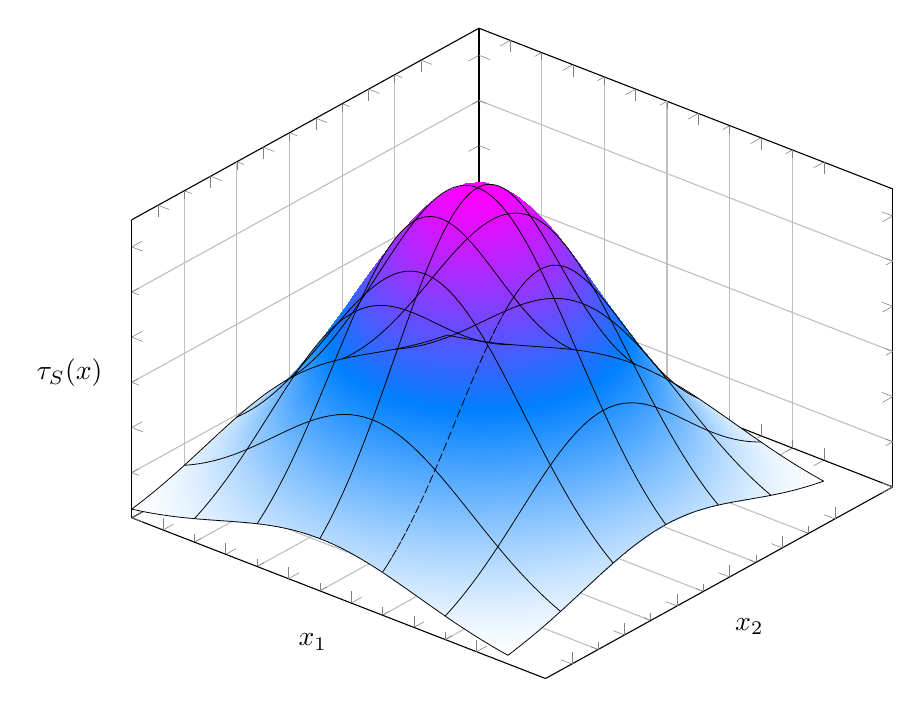
\begin{tikzpicture}
     \begin{axis}[
            view={40}{40},
          %x dir=reverse,
          %y dir=reverse,
          width=320pt,
          height=280pt,
          mesh,
          colormap/cool,
          %mesh/ordering=x varies,
          z buffer=auto,%reverse xy seq,
          xmin=-0.5,xmax=5.5,
          ymin=-0.5,ymax=5.5,
          zmin=0,zmax=0.3,
          enlargelimits=upper,
          xtick=data,
          extra tick style={grid=major},
          ytick={0,...,5},xtick={0,...,5},
          grid=minor,
          xticklabels=\empty,
          yticklabels=\empty,
          zticklabels=\empty,
          xlabel={$x_1$},
          ylabel={$x_2$},
          zlabel={$\tau_S(x)$},
          zlabel style={rotate=-90},
          minor tick num=1,
          samples=70]
        \addplot3[surf, domain=-0.5:5.5, shader=interp] {0.35*(exp(-0.2*(x-2.5)*(x-2.5)-0.2*(y-2.5)*(y-2.5))};
        \foreach \xx in {-0.5,0.5,...,5.5}
        {
          \addplot3+[domain=-0.5:5.5, line width=0.1mm, mark=none, color=black, samples y=0]
           ({\xx}, {x}, {0.35*(exp(-0.2*(\xx-2.5)*(\xx-2.5)-0.2*(x-2.5)*(x-2.5))});
        }

        % y=constant grids lines
        \foreach \yy in {-0.5,0.5,...,5.5}
        {
           \addplot3[domain=-0.5:5.5, line width=0.1mm, mark=none, color=black, samples y=0]
           ({x}, {\yy}, {0.35*(exp(-0.2*(x-2.5)*(x-2.5)-0.2*(\yy-2.5)*(\yy-2.5))});
        }

  
     \end{axis}
  \end{tikzpicture}
  \DIFdelbeginFL %DIFDELCMD < \vspace*{2px}
%DIFDELCMD <   %%%
\DIFdelendFL \DIFaddbeginFL \vspace{-10pt}
  \DIFaddendFL \caption[Example of an arbitrary mass-energy density]{An example of an arbitrary mass-energy density $\tau_S$ plotted against two dimensions $x_1$ and $x_2$ belonging to the hypersurface $S$. }\label{tauSexample}
  \end{figure}

  \begin{figure}[ht!]
    \captionsetup{justification=justified}
    \centering

    \pgfmathsetmacro{\gconv}{2*326.32446}
    % from https://tex.stackexchange.com/a/435234/121799
    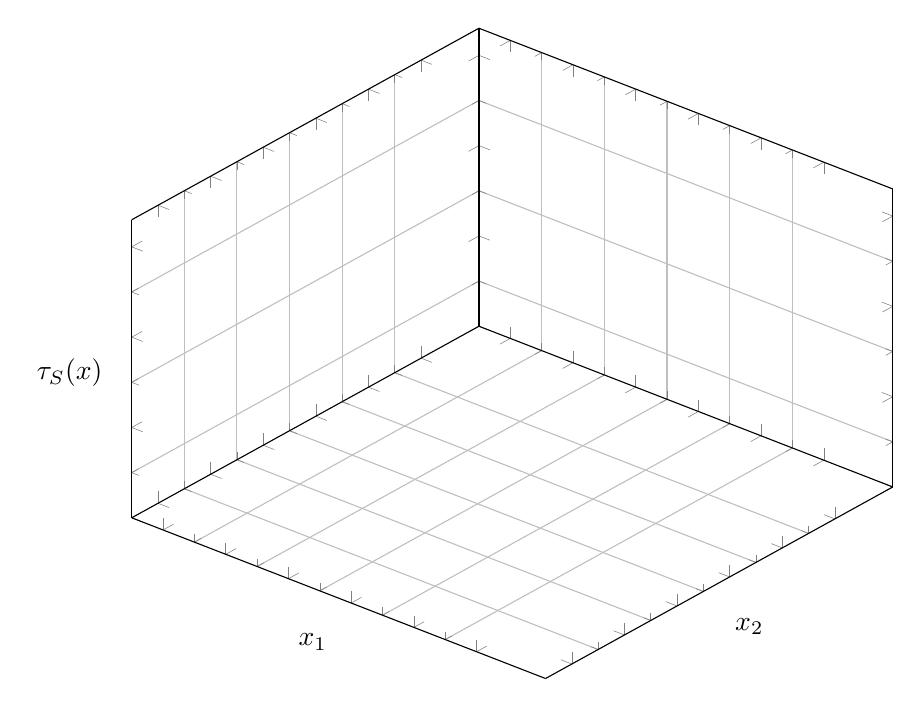
\begin{tikzpicture}[declare function={% (0.00001*\n!/(0.01*\x!*0.01*\y!*0.01*(\n-\x-\y)!))*
    f(\x,\y,\px,\py,\n)=(0.000001*\n!/(0.01*\x!*0.01*\y!*0.01*(\n-\x-\y)!))*pow(\px,\x)*pow(\py,\y)*pow(1-\px-\py,\n-\x-\y);}] % 
    \pgfplotsset{set layers}
    \begin{axis}[% from section 4.6.4 of the pgfplotsmanual
            view={40}{40},
            %x dir=reverse,
            %y dir=reverse,
            width=320pt,
            height=280pt,
            mesh,
            %mesh/ordering=x varies,
            z buffer=auto,%reverse xy seq,
            xmin=-0.5,xmax=5.5,
            ymin=-0.5,ymax=5.5,
            zmin=0,zmax=0.3,
            enlargelimits=upper,
            xtick=data,
            extra tick style={grid=major},
            ytick={0,...,5},xtick={0,...,5},
            grid=minor,
            xticklabels=\empty,
            yticklabels=\empty,
            zticklabels=\empty,
            xlabel={$x_1$},
            ylabel={$x_2$},
            zlabel={$\tau_S(x)$},
            zlabel style={rotate=-90},
            minor tick num=1,
            ]

      \addplot3 [point meta=0,visualization depends on={
      \gconv*z \as \myz}, % you'll get told how to adjust the prefactor
      scatter/@pre marker code/.append style={/pgfplots/cube/size z=\myz},%
      scatter/@pre marker code/.append style={/pgfplots/cube/size x=24.3018pt},%
      scatter/@pre marker code/.append style={/pgfplots/cube/size y=21.71275pt},%
      scatter,only marks,
      mark=my cube*,mark size=5,opacity=1,domain=0:5,domain y=0:5,samples=6,samples y=6]
      {0.35*(exp(-0.2*(x-2.5)*(x-2.5)-0.2*(y-2.5)*(y-2.5))};
        \end{axis}
    \end{tikzpicture}
    \DIFdelbeginFL %DIFDELCMD < \vspace*{2px}
%DIFDELCMD <     %%%
\DIFdelendFL \DIFaddbeginFL \vspace{-10pt}
    \DIFaddendFL \caption[Approximated arbitrary mass-energy density]{Here, the arbitrary mass-energy density $\tau_S$ depicted in figure \ref{tauSexample} has been approximated by a function which is constant in each mesh cell.}\label{tauSapprox}
    \end{figure}
    We can then suppose that with a suitably fine mesh\label{meshref} on $S$,\footnote{Note that the mesh is only a mesh in $S$, so the cells of the mesh are cube-like subsets of $S$. The time might not be constant across each cell because of the possible curvature of $S$.} any mass energy density $\tau_S(x)$ (e.g. such as the one depicted in figure \ref{tauSexample}) can be approximated to a function (e.g. like the one depicted in figure \ref{tauSapprox}) that has constant values on each cell of this mesh and such that the approximation value at a cell belongs to a finite pool of possible values. For instance, if $c_x$ is the cell which contains $x\in S$, and $\tau_{\text{max}}$ is the maximum possible value the mass-energy density could be, then we could define the approximation to $\tau_S(x)$ at cell $c_x$ to be
    \begin{equation}\label{tauapproxformula}
    \tau_S(c_x)=\frac{\tau_{\text{max}}}{N}\floor*{N\Big(\frac{\text{average of }\tau_S\text{ over }c_x}{\tau_{\text{max}}}\Big)+0.5}
    \end{equation}
    where $\floor*{z}$ is the biggest integer $n\leq z$, and where $N$ is a fixed large number. Then $\tau_S(c_x)$ will have $N+1$ possible values between $0$ and $\tau_{\text{max}}$.  There will then only need to be a countable number of approximations $\tau_{S,i}$ to approximate any arbitrary mass-energy density $\tau_S$ on $S$.  As long as we choose the cells in the mesh to be sufficiently small and $N$ to be sufficiently large, we can describe physical reality up to our desired level of accuracy. Thus, we assume that for each of the countable states in the orthonormal basis $\{\ket*{\Gamma_{i}}:i\in\mathbb{N}\}$, there will be a corresponding function $\tau_{S,i}$ defined on $S$ which is constant on every cell of $S$ and in which 
\begin{equation}\label{approxeigen}
\hat{T}_S(c_x)\ket*{\Gamma_{i}}= \tau_{S,i}(c_x)\ket*{\Gamma_{i}}
\end{equation} 
for all $x\in S$ where $ \tau_{S,i}(c_x)= \tau_{S,i}(x)$ and where $\hat{T}_S(c_x)$ is the observable corresponding to the average approximated value of the physical quantity $T_S(x)$ over the cell $c_x$ (approximated as in (\ref{tauapproxformula}) with $\tau_S$ replaced by $T_S$), but we will normally just write
\begin{equation}\label{approxeigen2}
  \hat{T}_S(x)\ket*{\Gamma_{i}}= \tau_{S,i}(x)\ket*{\Gamma_{i}}
  \end{equation}
with the implicit understanding that by (\ref{approxeigen2}) we really mean (\ref{approxeigen}), and that when we speak of $\ket*{\Gamma_{i}}$ and $\tau_{S,i}$ as simultaneous $\hat{T}_S$-eigenstates and simultaneous $\hat{T}_S$-eigenvalues respectively, we implicitly understand $\hat{T}_S$ and $\tau_{S,i}$ to be defined over cells of the form $c_x\subset S$ rather than over spacetime locations $x\in S$.

Now the additional variables beyond standard quantum theory that are included in Kent's theory are given by one of these simultaneous $\hat{T}_S$-eigenvalues $\tau_{S,i}$ that (approximately) describe a possible outcome for a mass-energy density measurement over the whole of $S$. We will let $\tau_S$ denote the particular  $\tau_{S,i}$ that constitute the additional variables of Kent's theory. 

Now the particular density $\tau_S$ which is found to describe $S$ can't be absolutely anything. Limitations are placed on what $\tau_S$ can be, and these limitations will depend on the initial conditions of Kent's theory. Kent assumes that all physics that we wish to describe takes place between two hypersurfaces $S_0$ %
\nomenclature{$S_0$}{Initial hypersurface for which Kent assumes all physics occurs between $S_0$ and $S$, \nomrefpage}%
 and $S$, with $S_0$ much earlier than $S$ so that $S_0$ and $S$ don't intersect. Initial conditions are determined on the hypersurface $S_0$ so that we can assume it is described by a state $\ket*{\Psi_0}\in H_{S_0}$ in the Tomonaga-Schwinger picture. %
 \nomenclature{$\ket*{\Psi_0}$}{The state of the initial hypersurface $S_0$ in the Tomonaga-Schwinger picture, \nomrefpage}% 
 If we  define 
\begin{equation}\label{SchwingerUnitaryOP}
U_{SS_0}=U[S]U[S_0]^{-1},
\end{equation} 
where $U[S]$ and $U[S_0]$ are the Schwinger unitary operators introduced on
 page \pageref{SchwingerOperator}, then
 given the state $\ket*{\Psi_0}$, there will be a corresponding state $\ket*{\Psi_S}=U_{SS_0}\ket*{\Psi_0}\in H_S$  %
 \nomenclature{$\ket*{\Psi_S}$}{The state $U_{SS_0}\ket*{\Psi_0}\in H_S$ in the Tomonaga-Schwinger picture, \nomrefpage}%
  that describes the hypersurface $S$ in the Tomonaga-Schwinger picture. Figure \ref{S1} depicts the evolution of the state $\ket*{\Psi_0}$ to the state $\ket*{\Psi_S}$.
  \begin{figure}[ht!]
    \captionsetup{justification=justified}
    \centering

    \tikzmath{
    \a= 1;  
    \h=-1;
    \md = (\a+\h)/2;
    \lrange = 4;
    \rrange=2;
    \fictlabel=(\rrange-\lrange)/2;
    \tlen=0.75;
    \labelpos=(-\lrange-\a)/2;
    } 

    \begin{tikzpicture}[thick, scale=2]
    \def\dotsize{0.7}
    \definecolor{tempcolor}{RGB}{0,151,76}
    \draw[<->] (-\lrange, \h) node[left] {$S_0$} -- (\rrange, \h) node[right] {$S_0$};
    \draw[<->](-\lrange, \a) node[left] {$S$} --  (\rrange, \a)  node[right] {$S$};                   
    \draw[->] (\rrange,\md-\tlen/2) --  (\rrange,\md+\tlen/2) node[midway,right]{time}; 
    \coordinate[label = above: Notional Measurement of $T_S(x)$ on $S$]  (D) at (\fictlabel,\a+0.2); 
    \node (start) at (\labelpos,\h) [below] {Initial State $\ket*{\Psi_0}$};
    \node (final) at (\labelpos,\a) [below] {Unitary Evolution $\ket*{\Psi_S}=U_{SS_0}\ket*{\Psi_0}$};
    \draw [->, shorten <= 5pt] (start) [above] -- (final); 

    \end{tikzpicture}

    \DIFdelbeginFL %DIFDELCMD < \vspace*{2px}
%DIFDELCMD <     %%%
\DIFdelendFL \DIFaddbeginFL \vspace{-10pt}
    \DIFaddendFL \caption[Depiction of a notional measurement of $T_S(x)$]{A notional measurement of $T_S(x)$ is made for all $x\in S$. The simultaneous  $\hat{T}_S$-eigenstate $\ket*{\Gamma}$ with $\hat{T}_S(x)\ket*{\Gamma}=\tau_S(x)\ket*{\Gamma}$ is selected with probability $\abs{\mel{\Gamma}{U_{SS_0}}{\Psi_0}}^2$ $=\abs{\ip{\Gamma}{\Psi_S}}^2$. The values $\tau_S(x)$ obtained for $T_S(x)$ are then used to calculate the physical properties at the spacetime location $y$.  }
    \label{S1}
    \end{figure} Then if $\ket*{\Gamma}$ is a simultaneous  $\hat{T}_S$-eigenstate with $\hat{T}_S(x)\ket*{\Gamma}=\tau_S(x)\ket*{\Gamma}$, then the probability $P(\Gamma|\Psi_0)$ %
  \nomenclature{$P(\Gamma|\Psi_0)$}{The probability that  $S$ will be found to be in the state $\ket*{\Gamma}$ with mass-energy density $\tau_S(x)$ given that $S_0$ was initially in the state $\ket*{\Psi_0}$, see equation (\ref{bornrule}), \nomrefpage}%
  that $S$ will be found to be in the state $\ket*{\Gamma}$ given the initial state $\ket*{\Psi_0}$ describing $S_0$ will be given by the Born Rule (see page \pageref{bornrule}):    
  \begin{equation}\label{bornpsi}
    P(\Gamma|\Psi_0) = \abs{\mel{\Gamma}{U_{SS_0}}{\Psi_0}}^2=\abs{\ip{\Gamma}{\Psi_S}}^2
    \end{equation}
  It's  possible that there could be more than one simultaneous  $\hat{T}_S$-eigenstate  in  $H_S$ that has the simultaneous  $\hat{T}_S$-eigenvalue $\tau_S$, but it is the mass-energy density $\tau_S$ itself rather than one of the eigenstates with mass-energy density $\tau_S$ that constitute the additional variables that Kent adds to standard quantum theory. 

\DIFaddbegin {\interfootnotelinepenalty\DIFadd{=10000   }\DIFaddend Also note that  if every simultaneous $\hat{T}_S$-eigenstate $\ket*{\Gamma}$ with simultaneous $\hat{T}_S$-eigenvalue $\tau_S$ satisfies $\abs{\mel{\Gamma}{U_{SS_0}}{\Psi_0}}=0$, then by (\ref{bornpsi}), $\tau_S$ will have zero probability, and hence, it will not be a possible measurement outcome for $T_S$ given $\ket*{\Psi_0}$.\footnote{\label{discreteRV}When dealing with continuous random variables, if the probability of the random variable having a particular value is  zero, it does not follow that it is impossible for the random variable to have this value. However, in the case of discrete random variables,  if the probability of the random variable having a particular value is  zero, then it does  follow that it is impossible for the random variable to have this value. Because we are using (\ref{tauapproxformula}) to approximate the energy density, we can treat  $T_S$ as a discrete random variable, hence the claim that if $T_S=\tau_S$ has zero probability,  then $\tau_S$ will not be a possible measurement outcome for $T_S$ given $\ket*{\Psi_0}$.} It is for this reason that we can't expect the measurement outcome of $T_S$ on $S$ to be absolutely anything.\DIFaddbegin }
\DIFaddend 










 








% flatex input end: [Chapter03/AdditionalVariables.tex]

%\usepackage[inline]{showlabels}
% flatex input: [Chapter03/OneWorldFeature.tex]

\section{The One-World Feature of Kent's Theory\DIFdelbegin %DIFDELCMD < \label{OneWorldFeature}%%%
\DIFdelend }\DIFaddbegin \label{OneWorldFeature}
\DIFaddend The third similarity Kent's theory shares with the Bohmian interpretation is that it is a one-world interpretation of quantum physics. It will be helpful to contrast this with the many-worlds interpretation. 

 Unlike the many-worlds interpretation, Kent's theory does not allow for indeterminate states of macroscopic objects such as cats. In the many-worlds interpretation, Schr\"{o}dinger will still only observe his cat to be either dead or alive, and not both dead and alive. However, Schr\"{o}dinger himself goes into a superposition of observing his cat to be alive and his cat to be dead. In the many-worlds interpretation, there is thus a difference between observing something to be so, and something actually being so: the observation is of a particular physical scenario, but the reality is a superposition of different physical scenarios. 

\DIFaddbegin {\interfootnotelinepenalty\DIFadd{=10000 }\DIFaddend To capture this distinction between observation and reality, Bell speaks of \textbf{beables}\index{beable}.\label{beabledef} Bell introduces the term beable when speculating on what would be a more satisfactory physical theory than what quantum physics currently has to offer.\footnote{See \cite{Bell2}\DIFaddbegin \DIFadd{.}\DIFaddend } Bell says that such a theory should be able to say of a system not only that such and such is observed to be so, but that such and such be so. In other words, a more satisfactory theory would be a theory of beables rather than a theory of observables. On the macroscopic level, these beables should be the underlying reality that gives rise to all the familiar things in the world around us, things like cats, laboratories, procedures, and so on. For example proponents of the Bohmian interpretation believe that the beables are all the particles each with their precise position and momentum. But whatever these beables are, it is because of them that a scientist can observe a physical system to be in such and such a state. Thus, observables are ontologically dependent on beables.   \DIFaddbegin }
\DIFaddend 

Now the beables in Kent's one-world interpretation are expressed in terms of a physical quantity called the \textbf{stress-energy tensor}\index{stress-energy tensor}  $T^{\mu\nu}(y)$.\label{stressenergy}   %
\nomenclature{$T^{\mu\nu}(y)$}{The stress-energy tensor, \nomrefpage}%
For any spacetime location $y$, the stress-energy tensor $T^{\mu\nu}(y)$ is an array of 16 values corresponding to each combination of $\mu, \nu=0,1,2,$ or $3$. %
\nomenclature{$\mu, \nu$}{Generic indices of tensors, $\mu, \nu=0,1,2,$ or $3$, \nomrefpage}%
 The value $T^{00}(y)$ is the energy density at $y$ divided by $c^2$,\footnote{This is not to be confused with the mass-energy density $T_S(x)$ defined for $x$ on a hypersurface $S$. As will be shown in section \ref{LorentzInvariance},   all 16 elements of $T^{\mu\nu}(x)$ will typically be needed to calculate $T_S(x)$.} whereas the other values of $T^{\mu\nu}(y)$ indicate how much energy and momentum flow across different surfaces in the neighborhood of $y$. 



It was mentioned in the previous section that for any spacetime location $x\in S$,  there is an observable $\hat{T}_S(x)$ acting on $H_S$ corresponding to the mass-energy density $T_S(x)$ of the surface $S$ at $x$. It turns out that for any $\mu, \nu=0,1,2,$ or $3$, there is also an observable  $\hat{T}^{\mu\nu}(x)$ acting  %
\nomenclature{$\hat{T}^{\mu\nu}(x)$}{The observable corresponding to the stress-energy tensor $T^{\mu\nu}(y)$ in the Tomonaga-Schwinger picture, \nomrefpage}%
 on $H_S$, such that if $\ket*{\Gamma}\in H_S$ is a simultaneous eigenstate of $\hat{T}^{\mu\nu}(x)$ with eigenvalue $\tau^{\mu\nu}(x)$ for  %
\nomenclature{$\tau^{\mu\nu}(x)$}{For fixed $\mu,\nu$, the simultaneous eigenvalue for all $x\in S$ of a simultaneous eigenstate $\hat{T}^{\mu\nu}(x)$, \nomrefpage}%
 all $x\in S$, then $\ket*{\Gamma}$ corresponds to a state of $S$ in which $T^{\mu\nu}(x)$ is  $\tau^{\mu\nu}(x)$ for all $x\in S$.\footnote{Note however, that such a simultaneous eigenstate is only for a fixed choice of $\mu$ and $\nu$, since in general, $\hat{T}^{\mu\nu}(x)$ and $\hat{T}^{\mu'\nu'}(x)$ will not commute for $\mu\neq\mu'$ or $\nu\neq\nu'$. } Moreover, the observable $\hat{T}_S(x)$ is expressible in terms of the  $\hat{T}^{\mu\nu}(x)$-observables.\footnote{See section  \ref{LorentzInvariance} for an explanation for why this is so.}\textsuperscript{,}\footnote{As in (\ref{approxeigen2}), we have the same implicit understanding of $\hat{T}^{\mu\nu}(x)$ and $\tau^{\mu\nu}(x)$ as being defined over cells $c_x\subset S$ rather than at spacetime locations $x\in S$, though we will often speak of them as being defined at spacetime locations. }
Now the  beables in Kent's theory are defined at each spacetime location $y$ that occurs after $S_0$ and before $S$. For such a spacetime location $y$, the beables will be determinate values of the stress-energy tensor $T^{\mu\nu}(y)$, but calculated from the expectation of the observable $\hat{T}^{\mu\nu}(y)$ conditional on the mass-energy density $T_S(x)$ on $S$ being given by $\tau_S(x)$ for all the $x\in S$ that are outside the light cone of $y$. 

\DIFaddbegin {\interfootnotelinepenalty\DIFadd{=10000 }\DIFaddend Kent implicitly assumes that a specification of the stress-energy tensor $T^{\mu\nu}(y)$ for all spacetime locations $y$ between $S_0$ and $S$ will be sufficient to give a macroscopic description of physical reality between $S_0$ and $S$.\footnote{See \cite[2]{Kent2014} where he talks about giving a description of reality between $S_0$ and $S$.} This seems like a reasonable assumption, since from the $T^{00}(y)$ component of the stress-energy tensor, we will be able to tell how much energy is present in the vicinity of $y$, and from the other components of the stress-energy tensor, we will be able to work out how much of this energy is due to mass and how much is due to motion.\footnote{It doesn't matter that the  $\hat{T}^{\mu\nu}(y)$ won't typically commute for all $\mu$ and $\nu$ because the value of $T^{\mu\nu}(y)$ that Kent ascribes to the spacetime location $y$ is not the eigenvalue of some simultaneous eigenstate of the $\hat{T}^{\mu\nu}(y)$ for all $\mu$ and $\nu$ (non-commutativity of the $\hat{T}^{\mu\nu}(y)$ would guarantee that there is no such simultaneous eigenstate). Rather, the value of $T^{\mu\nu}(y)$ that Kent ascribes to the spacetime location $y$ is an expectation value of  $\hat{T}^{\mu\nu}(y)$ conditioned on the mass-energy density $T_S(x)$ on $S$, and so the non-commutativity of the $\hat{T}^{\mu\nu}(y)$ is irrelevant when calculating this expectation value  for all $\mu$ and $\nu$. Nevertheless, one might still wonder whether it is sensible to ascribe the   expectation value of  $\hat{T}^{\mu\nu}(y)$ conditioned on the mass-energy density $T_S(x)$ on $S$ to $T^{\mu\nu}(y)$. But as we will see in section \ref{KentconsistentQT}, conditioning the expectation of $\hat{T}^{\mu\nu}(y)$ on the mass-energy density $T_S(x)$ on $S$ is equivalent to taking the expectation $\ev*{ \hat{T}^{\mu\nu}(y)}{\Gamma}$ defined in the usual way, where the conditioning is now encapsulated in $\ket*{\Gamma}$ (which I refer to as the conditioned quantum state). Moreover, we should typically expect there to be sufficient information in the mass-energy density $T_S(x)$ on $S$ to ensure that $\ket*{\Gamma}$ is very close to being an eigenstate of all the $\hat{T}^{\mu\nu}(c_y)$ where $\hat{T}^{\mu\nu}(c_y)$ is the averaged stress-energy operator over some mesoscopic three-dimensional spatial cell $c_y$ containing the spacetime location $y$ (i.e.  $\hat{T}^{\mu\nu}(c_y)=\frac{1}{|c_y|}\int_{y'\in c_y} \hat{T}^{\mu\nu}(y')\dd y'$ where $|c_y|$ is the volume of the  three-dimensional spatial cell $c_y$). This means there will be numerical quantities $t^{\mu\nu}$ for all $\mu$ and $\nu$ such that $\hat{T}^{\mu\nu}(c_y)\ket*{\Gamma}\approx t^{\mu\nu}\ket*{\Gamma}$ to very good approximation,  and the conditioned expectation value of $\hat{T}^{\mu\nu}(y)$ will thus be $\ev*{ \hat{T}^{\mu\nu}(c_y)}{\Gamma}\approx t^{\mu\nu}.$   The $t^{\mu\nu}$-values that approximate the  conditioned expectation value of $\hat{T}^{\mu\nu}(c_y)$ will then form a  good approximation of the average stress-energy tensor in the vicinity of $y$ at the macroscopic level.} Thus, from the stress-energy tensor, we will be able to form a picture of where things are and whether things are in equilibrium or whether there are flows of matter and energy from one region to another. Such a description of reality will also include information about measurement readings that scientists observe when performing their experiments, so although  we wouldn't expect there to be a complete specification of physical reality down to the microscopic level in terms of the stress-energy tensor, there will be enough information in the stress-energy tensor at the macroscopic level to make various scientific claims about physical reality at the microscopic level.  \DIFaddbegin }
\DIFaddend 

In section \ref{kentcalculation}, we will come back to the question of why we can't include any information about $\tau_S(x)$ for $x\in S$ within the light cone of $y$ when we discuss how the conditional expectations of the stress-energy density are calculated. But before we do that, we first consider why we should need conditional expectations at all in order to provide a one-world description of reality.


To this end, we recall the definition of expectation in equation (\ref{expectation2}) and the expectation formula (\ref{evev}) for an observable. In a theory that posited the beables to be the expectation values of $\hat{T}^{\mu\nu}(y)$ for any $y$ located between $S_0$ and $S$  without conditioning on the value of the mass-energy density $T_S$ on $S$, then the $T^{\mu\nu}(y)$-beable would just be $\ev*{\hat{T}^{\mu\nu}(y)}{\Psi_{S'}}$ where $\ket*{\Psi_{S'}}=U_{S'S_0}\ket*{\Psi_0}$ for any hypersurface $S'$ that goes through $y$.\footnote{This can be done such that $\ev*{\hat{T}^{\mu\nu}(y)}{\Psi_{S'}}$ does not depend on the hypersurface $S'$ other than the fact that it contains $y$. For more details see \cite{SchwingerJulianI}.} However,\DIFaddbegin \phantom{\footnotemark}\footnotetext{ \DIFadd{Original by Dhatfield. This image is licensed under the Creative Commons Attribution-Share Alike 3.0 Unported license. Source: https://commons.wikimedia.org/wiki/File:Schrodingers\_cat.svg.}}\DIFaddend such a beable would give a description of reality that was very different from what we observe. For instance, in a Schr\"{o}dinger cat-like experiment (see section \ref{SchrondingersCat}), there would be a stress-energy tensor distribution corresponding to both the cat being alive and the cat being dead in the same world as depicted in figure \ref{deadlivecat2}.
\begin{figure}[ht!] 
  \captionsetup{justification=justified}
  \centering
  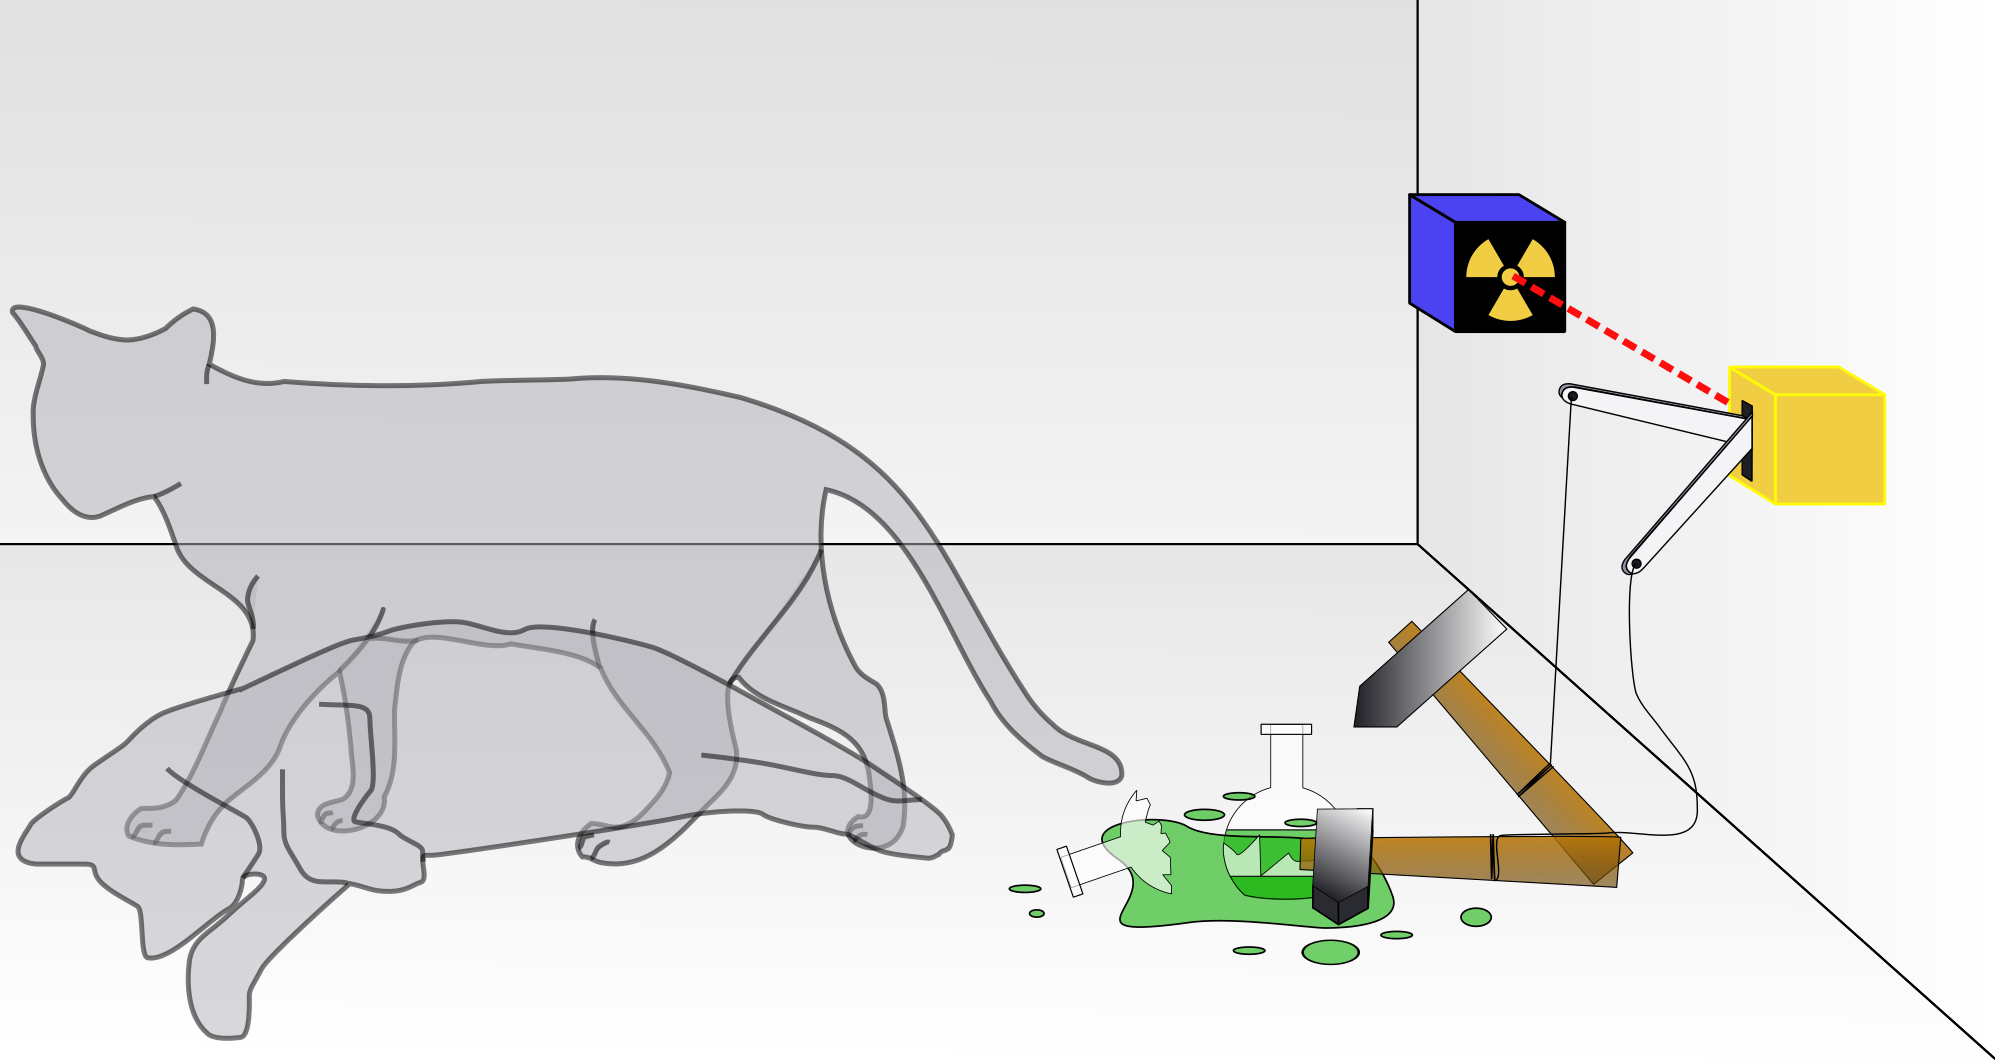
\includegraphics[width=100mm]{Chapter03/Schrodingers_cat.png}
  \caption[Depiction of Schr\"{o}dinger's cat]{A depiction of Schr\"{o}dinger's cat being both dead and alive.\protect\DIFdelbeginFL %DIFDELCMD < \footnotemark%%%
\DIFdelendFL \DIFaddbeginFL \footnotemark[\thefootnote]\DIFaddendFL }
  \label{deadlivecat2}
  \end{figure}
 \DIFdelbegin \footnotetext{\DIFdel{Original by Dhatfield. This image is licensed under the Creative Commons Attribution-Share Alike 3.0 Unported license. Source: https://commons.wikimedia.org/wiki/File:Schrodingers\_cat.svg}}
  %DIFAUXCMD
\DIFdelend \DIFaddbegin {\interfootnotelinepenalty\DIFadd{=10000  }\DIFaddend Such a distribution arises in this context because initially there is an atom that is in a superposition of decayed and non-decayed states, and so the expectation of $\hat{T}^{\mu\nu}(y)$ will have non-zero components both in the location where the non-decayed atom would be, and also in the locations of the decayed atom and the particle the atom emitted. As the decayed atom part of the state interacts with the poison releasing device, this device will also enter into a superposition so that in both the location of the poison containing flask and in the locations of all the poison atoms in the container containing the cat and into which the poison is released, the expectation of $\hat{T}^{\mu\nu}(y)$ will have non-zero components. And then the cat will enter into a superposition of being in a dead state and an alive state, and so  the expectation of $\hat{T}^{\mu\nu}(y)$ will have non-zero components in locations where the dead cat ends up and where the living cat happens to be. So the expectation of $\hat{T}^{\mu\nu}(y)$ in the locations of the container containing the cat will be very different from what someone would actually observe. To see how bizarre a description of reality would be if we just based it on unconditioned expectation values of observables, suppose we had an observable $A$ whose value was $1$ if the cat was alive and $0$ if the cat was dead, then assuming the decay probability was $1/2$, the expected value of $A$ would be $1/2$. Therefore, if we were to rely on such an expectation value in describing physical reality, we would have to say that the cat was literally half-dead and half-alive. \DIFaddbegin }
\DIFaddend 

  To overcome this defect, information about the mass-energy density on $S$ is used, specifically the values of $\tau_S(x)$ for $x\in S^1(y)$ where  $S^1(y)$  %
  \nomenclature{$S^1(y)$}{The set  of all the spacetime locations of $S$ outside the light cone of $y$, \nomrefpage}%
  is defined to consist of all the spacetime locations of $S$ outside the light cone of $y$ as depicted in figure \ref{S2}.  
 \DIFdelbegin %DIFDELCMD < 

%DIFDELCMD <  %%%
\DIFdelend \begin{figure}[ht!]
\captionsetup{justification=justified}
\centering

\tikzmath{
\a= 1;  
\e = 0.1;
\h=-1;
\hae=(3*\a*\a+6*\a*\e+7*\e*\e-3*\a*sqrt(\a*\a+4*\e*\e)-4*\e*sqrt(\a*\a+4\e*\e))/(4*\a+4*\e-2*sqrt(\a*\a+4*\e*\e));
\hae=0.0463647;
\hae=0.0858615;
\circsize=1.2;
\md = (\a+\h)/2;
\lrange = 4;
\rrange=2;
\ss=(-\lrange-\a)/2;
\sss=\a+(\rrange-\a)/2;
\tlen=0.75;
\labelpos=(-\lrange-\a)/2;
} 

\begin{tikzpicture}[thick, scale=2]

\def\dotsize{0.7}

\definecolor{tempcolor}{RGB}{0,151,76}
\draw[<->] (-\lrange, \h) node[left] {$S_0$} -- (\rrange, \h) node[right] {$S_0$};
\filldraw (0,0) circle (\dotsize pt) node [below right] {$y$} ;



\draw[<-] (-\lrange, \a)  -- (-\a, \a)  {};
\draw[gray, dotted] (-\a, \a) -- (0,0) {};
\draw[gray, dotted](0,0) -- (\a, \a) {};
\draw[->](\a, \a) --  (\rrange, \a)  ;         
\coordinate (B) at (\a,\a);
\node at (B)[red,circle,fill,inner sep=\circsize pt]{};
\coordinate (A) at (-\a,\a);
\node at (A)[red,circle,fill,inner sep=\circsize pt]{};
\coordinate (C) at (0,0);
\node at (C)[black,circle,fill,inner sep=\circsize pt]{};



\coordinate[label = above:$S^1(y)$]  (D) at (\ss,\a);
\coordinate[label = above:$S^1(y)$]  (D) at (\sss,\a);

\draw[->] (\rrange,\md-\tlen/2) --  (\rrange,\md+\tlen/2) node[midway,right]{time}; 

\node (start) at (\labelpos,\h) [below] {Initial State $\ket*{\Psi_0}$};
\node (evolution) at (\labelpos,\md+0.05) [below] {Unitary Evolution $U_{S'S_0}\ket*{\Psi_0}$};
\node (final) at (\labelpos,\a) [below] {Unitary Evolution $\ket*{\Psi_S}=U_{SS_0}\ket*{\Psi_0}$};
%\node at (-\ss+0.17,\mn-0.18){$-a_0$};
\draw [->, shorten <= 5pt] (start) [above] -- (evolution); 
\draw [->] (evolution) -- (final); 
\end{tikzpicture}
\DIFdelbeginFL %DIFDELCMD < 

%DIFDELCMD < \vspace*{2px}
%DIFDELCMD < %%%
\DIFdelendFL \DIFaddbeginFL \vspace{-10pt}
\DIFaddendFL \caption[Depiction of $S^1(y)$]{The set $S^1(y)$ consists of all the spacetime locations of $S$ outside the light cone of $y$. The $T^{\mu\nu}(y)$-beables are calculated using the initial state $\ket*{\Psi_0}$ together with the values of $\tau_S(x)$ for $x\in S^1(y)$. }
\label{S2}
\DIFaddbeginFL \vspace{12.96pt}
\DIFaddendFL \end{figure}
 So in the case of Schr\"{o}dinger's cat, if the cat were dead,  light reflecting off the dead cat and going off into outer space would eventually intersect the hypersurface $S$, and the light distribution on $S$ would register the inanimate status of the cat. On the other hand, if the cat were alive, the light reflecting off the living cat and going off into outer space would also intersect $S$, but now the light distribution on $S$ would register the different locations the living cat was in as it moved about. Because light travels at a constant speed in a vacuum, the state of the cat at earlier times would be described by light distributions in regions on $S$ that were further away from the cat than those light distributions in regions of $S$ that described the cat in more recent times. 

\DIFaddbegin {\interfootnotelinepenalty\DIFadd{=10000 }\DIFaddend Now if the cat was in a superposition of dead and alive states, then assuming there is no intermediate collapse of the global quantum state,  the hypersurface $S$ would also enter into a superposition of different states corresponding to these different distributions of light registered on $S$. But if a notional measurement on $S$ is made that determines which of these distributions is actually realized on $S$, then this determination will determine which history was actualized, and hence determine whether the cat actually survived Schr\"{o}dinger's experiment or whether it perished.   Thus, by conditioning on one of these two distributions on $S$ being actualized, the conditional expectation of the stress-energy tensor in the vicinity of where Schr\"{o}dinger's cat might be 
will not describe a situation like the one depicted in figure \ref{deadlivecat2}. \DIFaddbegin \begin{figure}[ht!]
  \captionsetup{justification=justified}
  \centering
  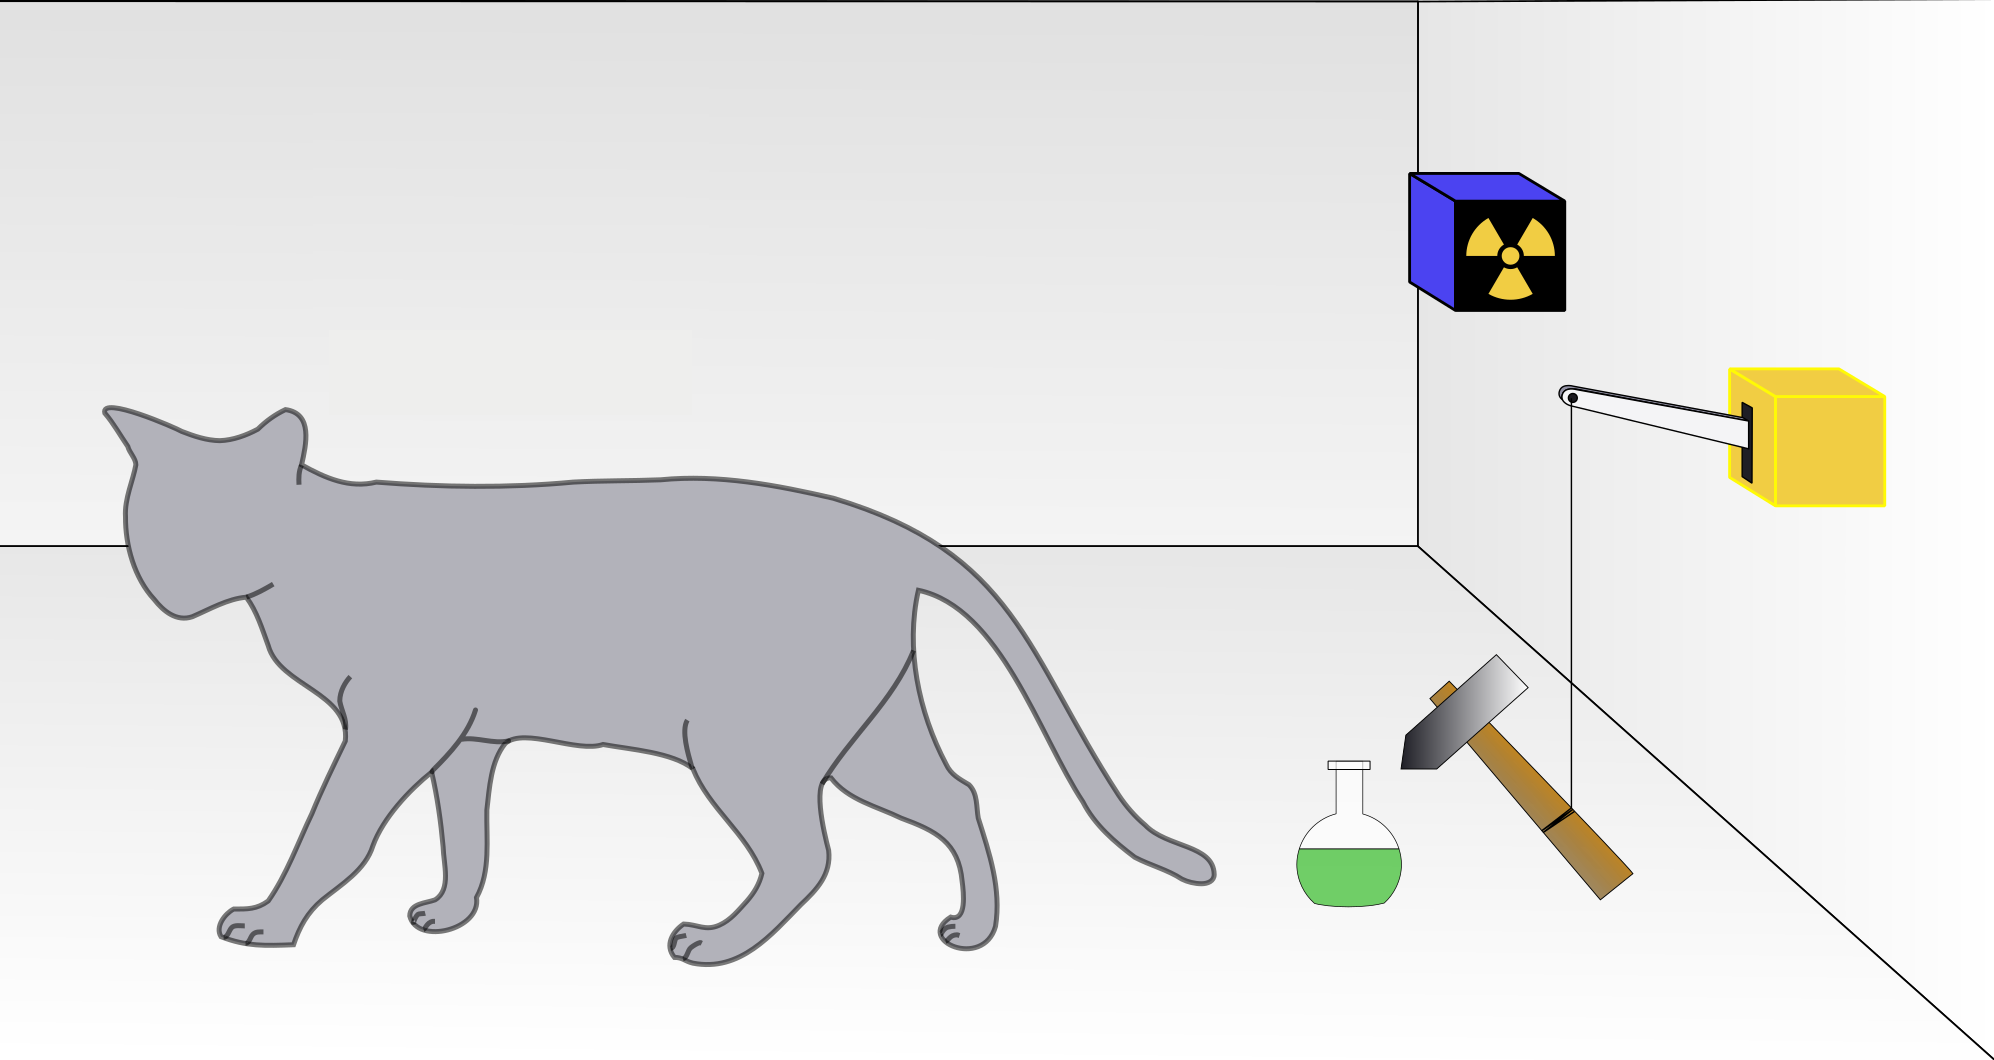
\includegraphics[width=100mm]{Chapter03/Schrodingers_livecat.png}
  \caption[Depiction of Schr\"{o}dinger's living cat]{\DIFaddFL{A depiction of Schr\"{o}dinger's cat being alive.}\protect\footnotemark}
  \label{livecat}
  \end{figure}
  \footnotetext{ \DIFadd{Original by Dhatfield. This image is licensed under the Creative Commons Attribution-Share Alike 3.0 Unported license. Source: https://upload.wikimedia.org/
  wikipedia/commons/archive/9/91/20080627113554!Schrodingers\_cat.svg.}}\DIFaddend Rather, it will either describe a situation like the one depicted in figure \ref{livecat}, or it will describe a situation like the one depicted in figure \ref{deadcat}. Which of these two situations occur will be determined by whether the measurement outcome on $S$ corresponds to a light distribution reflected from a living cat, or to a light distribution reflected from a dead cat. 
\DIFdelbegin %DIFDELCMD < \begin{figure}[ht!]
%DIFDELCMD <   \captionsetup{justification=justified}
%DIFDELCMD <   \centering
%DIFDELCMD <   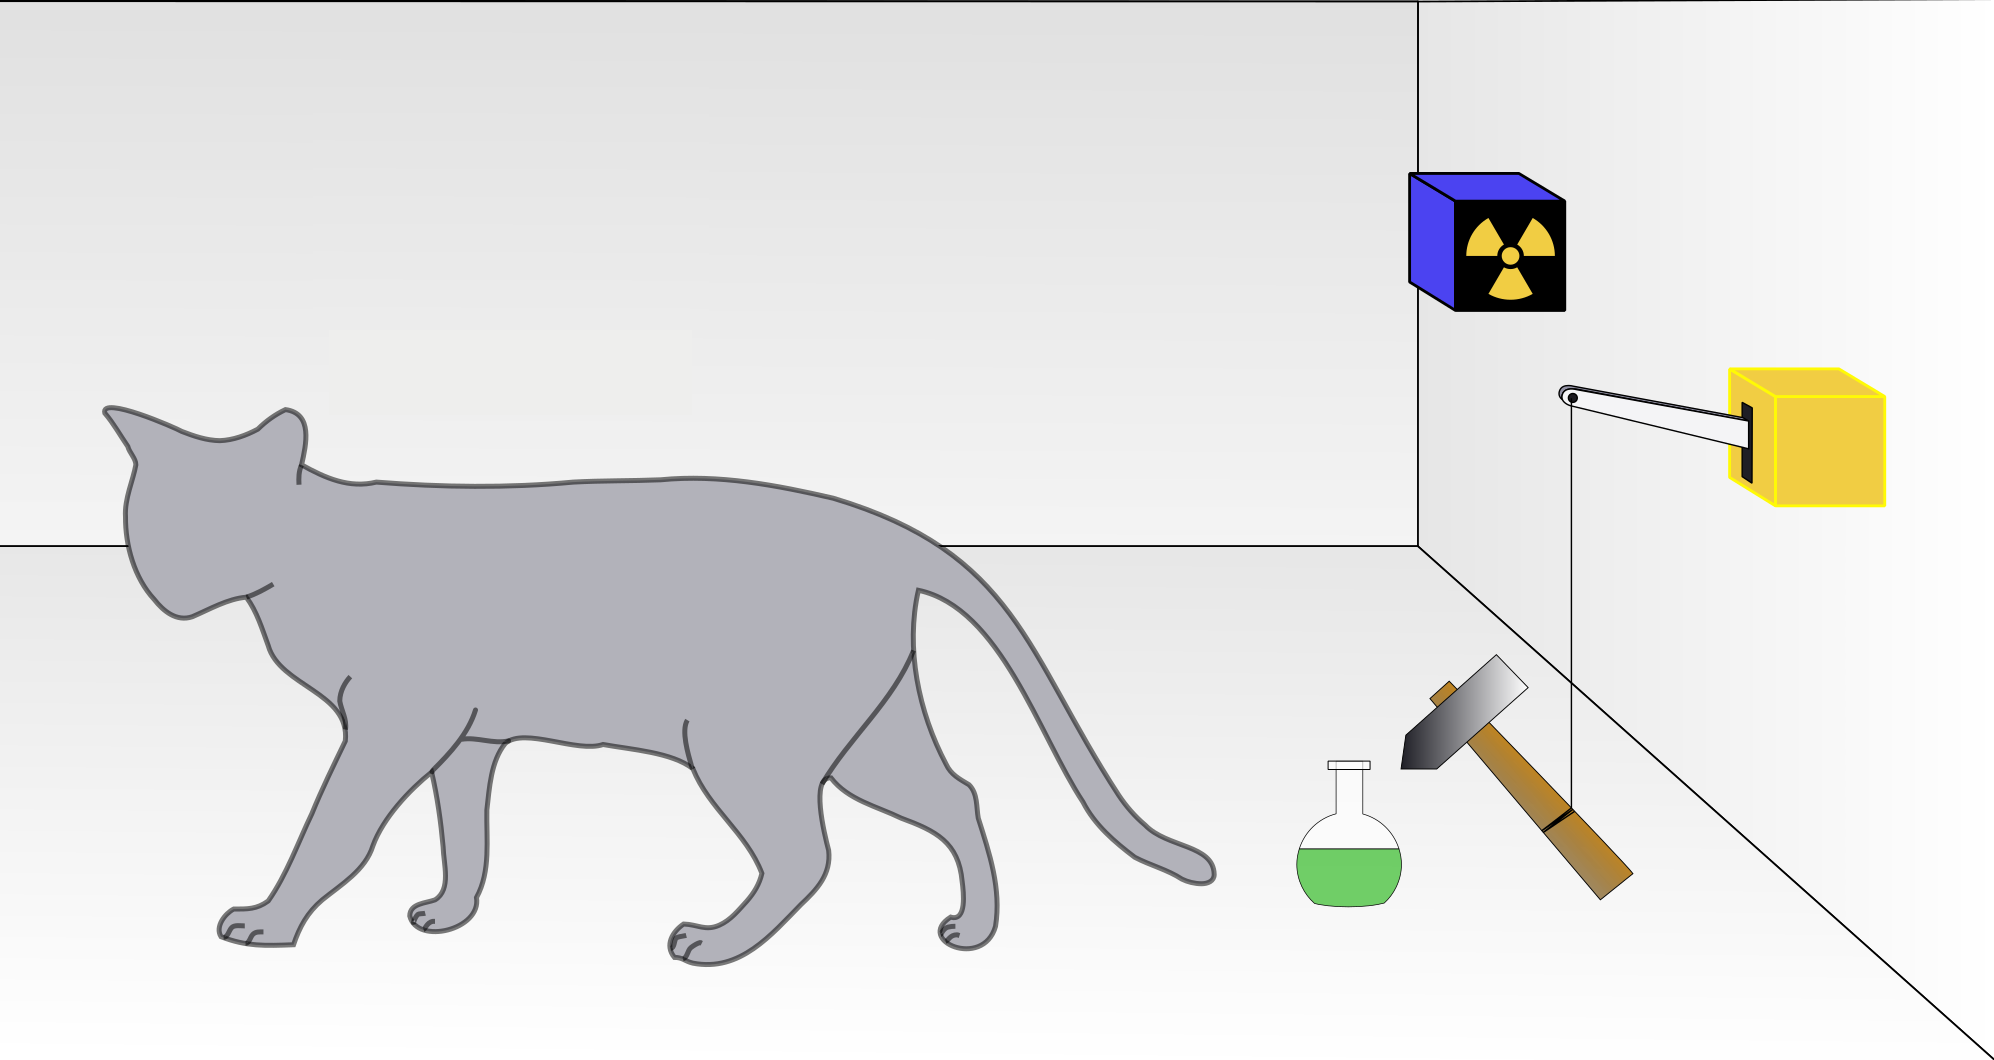
\includegraphics[width=100mm]{Chapter03/Schrodingers_livecat.png}
%DIFDELCMD <   %%%
%DIFDELCMD < \caption[Depiction of Schr\"{o}dinger's living cat]{%
{%DIFAUXCMD
\DIFdelFL{A depiction of Schr\"{o}dinger's cat being alive.}%DIFDELCMD < \protect\footnotemark%%%
}
  %DIFAUXCMD
%DIFDELCMD < \label{livecat}
%DIFDELCMD <   \end{figure}
%DIFDELCMD <   %%%
\footnotetext{\DIFdel{Original by Dhatfield. This image is licensed under the Creative Commons Attribution-Share Alike 3.0 Unported license. Source: https://upload.wikimedia.org/
  wikipedia/commons/archive/9/91/20080627113554!Schrodingers\_cat.svg}}
%DIFAUXCMD
\DIFdelend 

\DIFdelbegin %DIFDELCMD < \begin{figure}[ht!]
%DIFDELCMD <     \captionsetup{justification=justified}
%DIFDELCMD <     \centering
%DIFDELCMD <     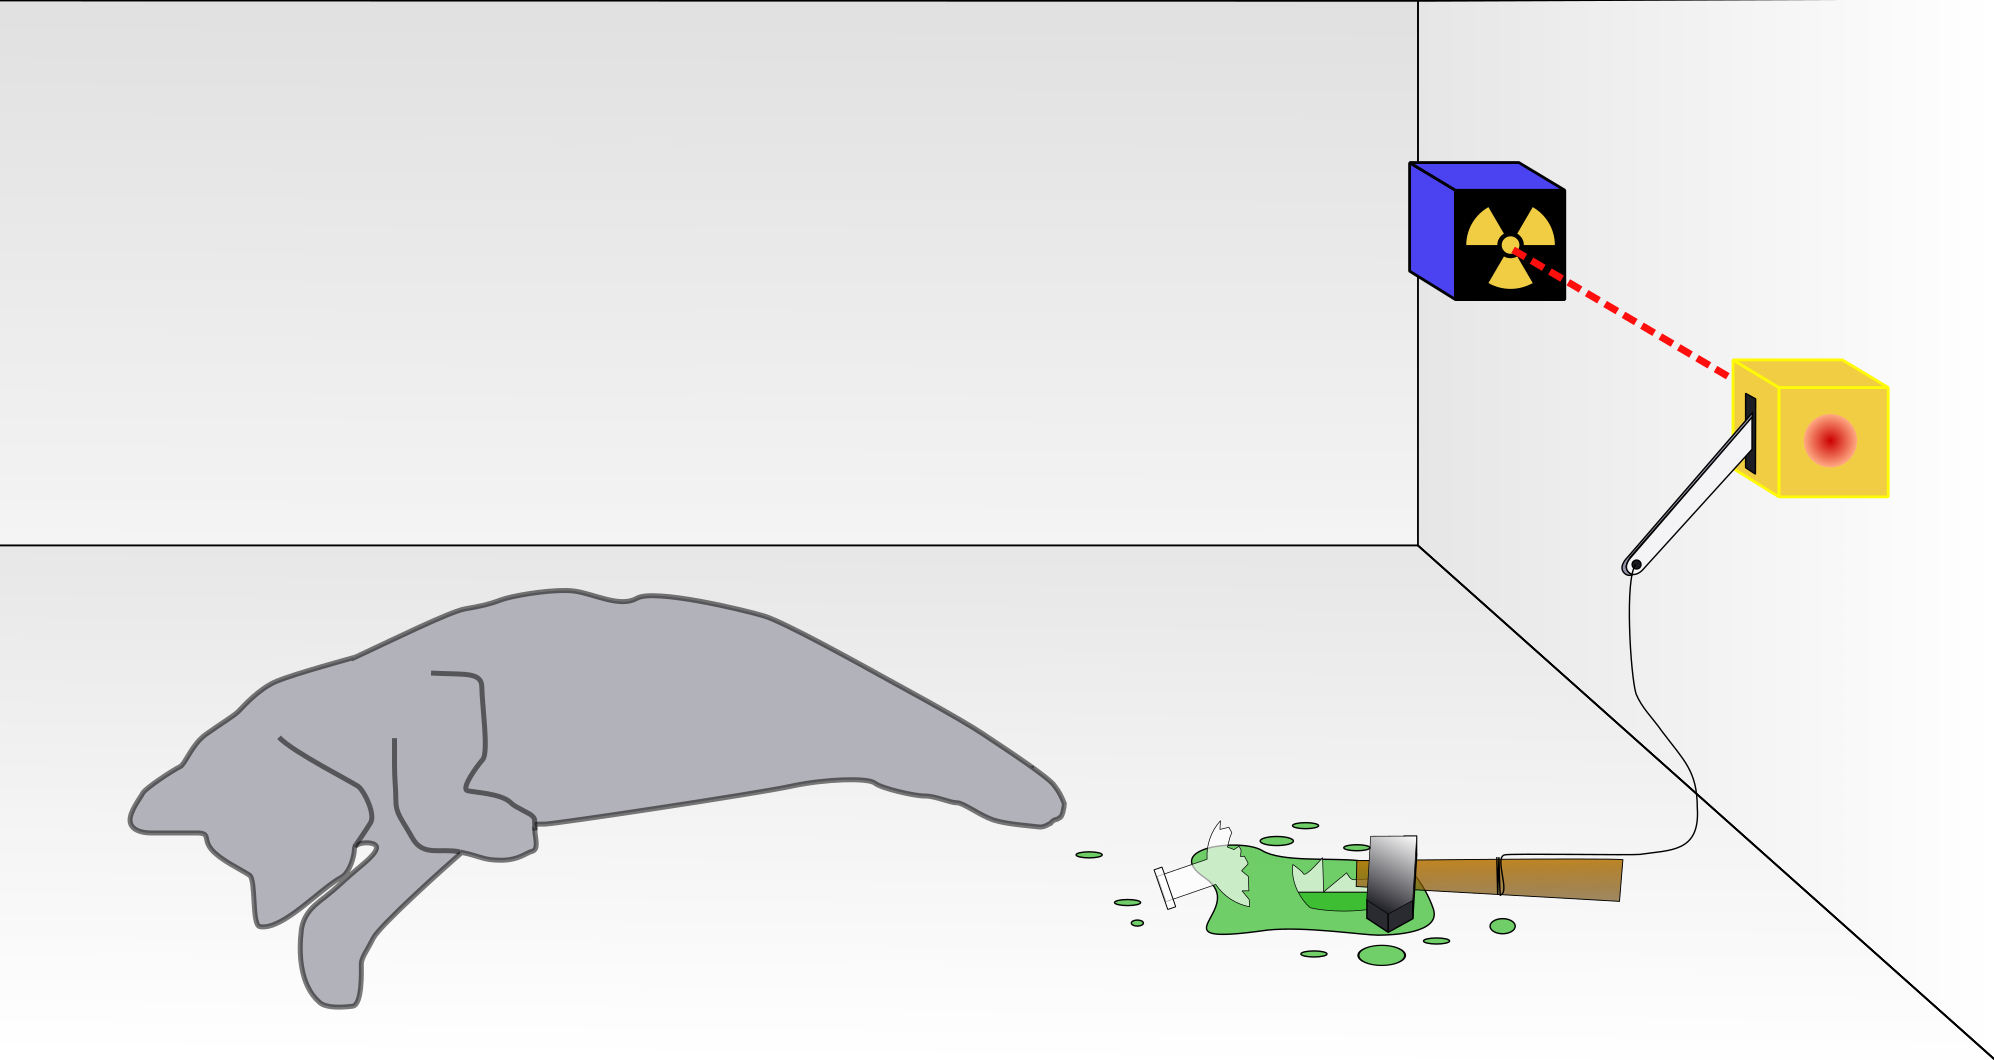
\includegraphics[width=100mm]{Chapter03/Schrodingers_deadcat.png}
%DIFDELCMD <     %%%
%DIFDELCMD < \caption[Depiction of Schr\"{o}dinger's dead cat]{%
{%DIFAUXCMD
\DIFdelFL{A depiction of Schr\"{o}dinger's cat being dead.}%DIFDELCMD < \protect\footnotemark%%%
}
    %DIFAUXCMD
%DIFDELCMD < \label{deadcat}
%DIFDELCMD <     \end{figure}
%DIFDELCMD < %%%
\footnotetext{\DIFdel{Original by Dhatfield. Altered by removing numbers and making into two separate figures. This image is licensed under the Creative Commons Attribution-Share Alike 3.0 Unported license. Source: https://upload.wikimedia.org/wikipedia/commons/archive/9/91/
20080627113554!Schrodingers\_cat.svg}} 
    %DIFAUXCMD
%DIFDELCMD < 

%DIFDELCMD < %%%
\DIFdelend One obvious objection to the above explanation is that one could imagine that the cat is in a box with perfectly mirrored walls, so that light from the cat can't escape. In such a situation, there would be no information about the cat's death or survival outside the relevant light cone, and so the cat would remain in a superposition of alive and dead states. Although perfectly mirrored walls are practically impossible, it would still seem rather problematic that the cat's having a well-defined life/death state depends on how perfectly reflective the walls of the box are. \DIFaddbegin }
\DIFaddend 

\DIFaddbegin \begin{figure}[ht!]
    \captionsetup{justification=justified}
    \centering
    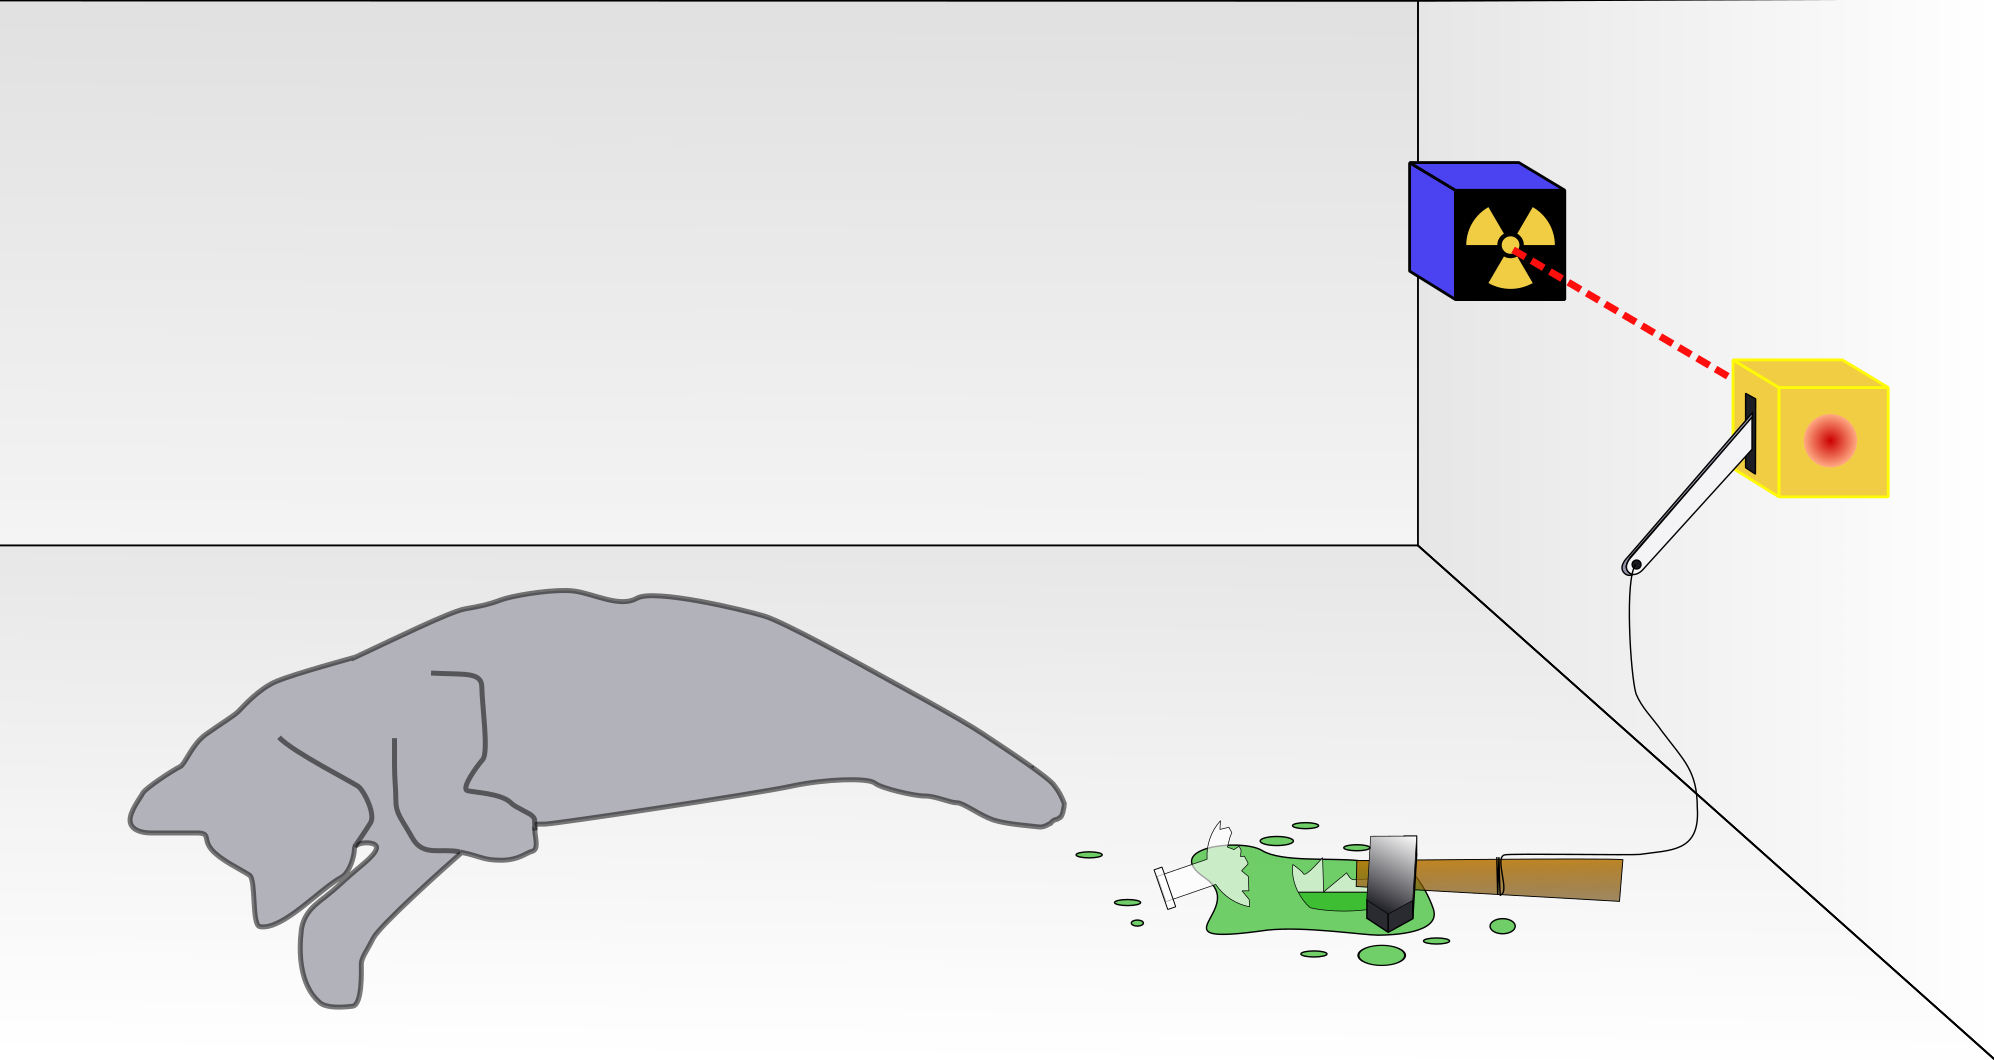
\includegraphics[width=100mm]{Chapter03/Schrodingers_deadcat.png}
    \caption[Depiction of Schr\"{o}dinger's dead cat]{\DIFaddFL{A depiction of Schr\"{o}dinger's cat being dead.}\protect\footnotemark}
    \label{deadcat}
    \vspace{-30pt}
    \end{figure}
\footnotetext{ \DIFadd{Original by Dhatfield. Altered by removing numbers and making into two separate figures. This image is licensed under the Creative Commons Attribution-Share Alike 3.0 Unported license. Source: https://upload.wikimedia.org/wikipedia/commons/archive/9/91/
20080627113554!Schrodingers\_cat.svg.}} 

\DIFaddend In responding to this objection, we should clarify that it is not necessary that light that has reflected directly off the cat must eventually intersect $S$ in order for the cat's state to be determined. Rather it is only necessary that light that has reflected off something that the cat is entangled with eventually intersects $S$. Now when light from the cat is reflected by the walls, the atoms in the walls affected by the light from the cat will get entangled with the cat, and the affected atoms will then interact with neighboring atoms which in turn will get entangled with the atoms that are entangled with the cat, and this entanglement will propagate through to the walls of the box, and when the light that reflects off the outside walls of the box is measured on $S$, this will contain some information about the state of the atoms of the outside walls and hence the atoms they are entangled with, and so this will ultimately lead to information about the state of the cat. 

One might still worry that it would still take a very long time for the light measured on $S$ to be sufficient to distinguish between the cat being alive and the cat being dead. We do however, have reason to think that this process might be very quick. For example, as already mentioned on page \pageref{electronspread},  if a free electron is initially described by a wave packet whose width is around $\du{e-10}{\m}$, then according to the Schr\"{o}dinger equation, after one second the width of the wave packet will have spread to a width of around $\du{1000}{\km}$. In reality, however, the electron remains relatively localized because of the scattering of light from the electron, and the light contains information that is able to localize the electron's position. So in the case of the cat in a box, the light reflecting off the outside of the box is at least going to contain enough information in the space of a second to determine that the cat is in the box rather than $\du{1000}{\km}$ away. And given that a cat is significantly larger than an electron, it seems very plausible that the light reflected off the outside of the box is going to contain significantly more information than the mere fact that the cat is in the box, and so we can reasonably expect there to be enough information in a short space of time to determine whether the cat is alive or dead.

    
\label{selectionmeaningbeg} Another objection one could raise against Kent's interpretation is that it depends on the selection of a particular measurement outcome $\tau_S$ for the mass-energy density $T_S$ on $S$. However, Kent is rather vague about what he means by selection. Here is a (slightly edited) passage from Kent's 2014 paper that could do with some clarification:
\DIFaddbegin \pagebreak
\DIFaddend \begin{adjustwidth}{1cm}{}
	\begin{displayquote}
    \DIFaddbegin \singlespacing
    \DIFaddend For any given hypersurface $S$ in the future of the initial hypersurface $S_0$, we consider the effect of joint measurements of the local mass-energy density $T_S(x)$ \ldots carried out at each point $x\in S$ \ldots. This gives us a probability distribution on possible mass-energy distributions $\tau_S(x)$ on $S$. In a universe in which physics starts on $S_0$ and ends on $S$, our picture of reality is that one $\tau_S(x)$ is randomly selected from the Born rule probability distribution. In other words, there is a randomly selected final boundary condition on S, which is defined mathematically in the same way that it would be if $T_S(x)$ were actually measured on S. However, we treat this simply as a mathematical algorithm. We do not suppose that a physical measurement actually takes place on $S$, or anywhere else. Our aim, instead, is to give a mathematical description of reality applicable to closed quantum systems, for which there are no external observers able to carry out measurements. To give a description of reality between $S_0$ and $S$, we use the initial state on $S_0$, the randomly chosen final outcome data $\tau_S(x)$ on $S$, and the unitary evolution law arising from the quantum dynamics.\footnote{\cite[2]{Kent2014}\DIFaddbegin \DIFadd{.}\DIFaddend }
  \end{displayquote}
\end{adjustwidth}  
Now this passage raises two questions. Firstly, there is the question of what it means for the final outcome data $\tau_S$ on $S$ to be \emph{selected}, and secondly, there is the question of what it means for the final outcome data $\tau_S$ on $S$ to be selected \emph{randomly from the Born rule probability distribution}. 

With regard to the question of what it means to be selected, some greater clarity would be desirable since there will be other possible outcomes each of which will also have data describing them. It would therefore be helpful to know what we mean by predicating `selected' of one possible set of outcome data $\tau_S$, and predicating `not selected' of another set of outcome data $\tau_S'$? Now one suggestion would be to say that the predicate `selected' just means the attribution of some kind of quality $Q_\text{selected}$ to the outcome data $\tau_S$ which the outcome data $\tau_S'$ lacks. However, if we took this suggestion seriously, it would not be obvious why the quality $Q_\text{selected}$ of $\tau_S$ is a reason to consider the universe $\mathcal{U}$  whose description between $S_0$ and $S$ depended on $\tau_S$ was any more real than  the universe $\mathcal{U}'$  whose description between $S_0$ and $S$ depended on $\tau_S'$. In this case, we might therefore doubt that Kent was really proposing a one-world interpretation of quantum physics. 


A better way to think of what was meant by predicating `selected' of $\tau_S$ would be to say that it just means that $\tau_S$ is a property of $S$, namely at each $x\in S$, the mass-energy density $T_S(x)$ is given by $\tau_S(x)$. Such an understanding of $\tau_S$ being selected would then be no more problematic than predicating properties of a subject. And since $\tau_S'$ is not a property of $S$, we would not be inclined to think that a universe $\mathcal{U}'$  whose description between $S_0$ and $S$ depended on $\tau_S'$ was real. 

With regard to the question of what it means for $\tau_S$ to be randomly selected from the Born rule probability distribution, if there is only one state $\ket*{\Gamma}$ such that $\hat{T}_S(x)\ket*{\Gamma}=\tau_S(x)\ket*{\Gamma}$ for all $x\in S$, then the probability $P(\tau_S)$ that $\tau_S$ is selected will be precisely the probability given by equation (\ref{bornpsi}). But if there are several states $\{\ket*{\Gamma_\alpha}:\alpha\}$ such that  $\hat{T}_S(x)\ket*{\Gamma_\alpha}=\tau_S(x)\ket*{\Gamma_\alpha}$, then the probability $P(\tau_S)$ that $\tau_S$ is selected will be 
\DIFdelbegin \begin{displaymath}\DIFdel{P(\tau_S)=\sum_\alpha \abs{\mel{\Gamma_\alpha}{U_{SS_0}}{\Psi_0}}^2=\sum_\alpha \abs{\ip{\Gamma_\alpha}{\Psi_S}}^2}\end{displaymath}%DIFAUXCMD
\DIFdelend \DIFaddbegin 

    \vspace{-37pt}%DIF > yyyyyyyyyyyyyyyyy
\begin{equation*}
\DIFadd{P(\tau_S)=\sum_\alpha \abs{\mel{\Gamma_\alpha}{U_{SS_0}}{\Psi_0}}^2=\sum_\alpha \abs{\ip{\Gamma_\alpha}{\Psi_S}}^2
    \vspace{-7.96pt}
}\end{equation*}\DIFaddend  
where $\ket*{\Psi_S}=U_{SS_0}\ket*{\Psi_0}$. However, although we can state the Born rule probability $P(\tau_S)$ for $\tau_S$ to be selected, this doesn't tell us what it \emph{means} for $\tau_S$ to be selected with this probability. Given that Kent is proposing a one-world interpretation, he is presumably not thinking of this probability in frequentist terms as though there were many worlds with a certain proportion of them having the mass-energy density $T_S$ being given by $\tau_S$. One could try to understand the probability $P(\tau_S)$ as making a counter-factual claim: if there were many worlds, then a certain proportion of them would have the mass-energy density $T_S$ being given by $\tau_S$. But such a counter-factual claim seems irrelevant to the manner in which $\tau_S$ is selected. If $\tau_S'$ was another possible mass-energy density such that $P(\tau_S)\ll P(\tau_S')$,  then despite this inequality, $\tau_S$ could still be selected so long as $P(\tau_S)>0$, and so in this case, to say $\tau_S$ was selected with probability $P(\tau_S)$ is not obviously saying anything more than  $\tau_S$ was selected.

Perhaps we could instead think of the probability $P(\tau_S)$ in Bayesian terms, that is, maybe we should think of $P(\tau_S)$ as expressing a degree of belief that $\tau_S$ is the mass-energy density $T_S$. But again there is the problem of relevance: what relevance is my degree of belief to the fact that $\tau_S$ is selected? Perhaps I will be extremely surprised to learn that $\tau_S$ is selected, but my surprise doesn't make any difference to the fact that $\tau_S$ is selected. From a Bayesian perspective, there is also the further problem that there is going to be so much information in $\tau_S(x)$, and $P(\tau_S)$ is going to be so small due to the vast number of possible values for $T_S$, and so what is being claimed about $\tau_S$ when saying it has a probability $P(\tau_S)$ would be beyond the comprehension of any human mind to form any definite beliefs. 

Another alternative for what it means for $\tau_S$ to be randomly selected from the Born rule probability distribution $P(\tau_S)$ would be to say there is some threshold $\epsilon>0$ such that if $P(\tau_S)\geq\epsilon$, then $\tau_S$ is a possible value for $T_S$, whereas if $P(\tau_S)<\epsilon$, then  $\tau_S$ is not a possible value for $T_S$. Presumably, we could make $\epsilon$ sufficiently large so as to avoid scenarios in which there were stress-energy tensor values in regions between  $S_0$ and $S$ which corresponded to a cat being both dead and alive. Perhaps making $\epsilon$ larger still would ensure that a world whose description depended on $\tau_S$ with  $P(\tau_S)>\epsilon$ and in which there were sufficiently intelligent scientists would be a world in which scientists could formulate the theory of quantum physics as we know it based on their experimental observations. However, one problem with this suggestion is that the smaller $\epsilon$ is, the less the Born rule has any bearing on which $\tau_S$ is selected. If we permitted $\epsilon=0$, then the Born rule would have no relevance at all. Also, it would seem strange to treat the selection of two possible mass-energy densities $\tau_S$ and $\tau_S'$ in exactly the same way if $P(\tau_S)\gg P(\tau_S')>\epsilon$. 

Another way of thinking about the probability $P(\tau_S)$ would be to take the metaphor of God throwing dice: God throws some dice many times, and based on the sum of the outcomes, He chooses one of the $\tau_S$ in such a way that more probable sums correspond to $T_S$-outcomes with greater Born rule probability. Given such a scenario, we would need to explain the association between dice throws and $T_S$-outcomes -- perhaps God has a huge library of books each of which specifies a different $T_S$-outcome, and that when God  has summed up all His dice throws, He selects the book that has the same catalog number as this sum. Then finally, God makes $S$ have the same $T_S$-value as specified in the book He selected. However, one reason for having misgivings about such a suggestion is that we might think that each of the books that was not selected could still be considered to be just as real as the world described by the book that God did select. Therefore, if Kent's interpretation required something analogous to these books to make sense of the Born rule probability, we might worry whether his interpretation  really was a one-world interpretation of quantum physics. 

But perhaps another way of associating dice throws with $T_S$-outcomes would be to suppose that God lays a mesh over $S$ and determines the mass-energy density of each cell of the mesh in turn by using the following strategy: He first selects one of the cells whose mass-energy density He hasn't already determined; He then rolls some dice, and He then uses an algorithm to calculate the mass-energy density of the cell He has just selected where the algorithm depends on the dice outcome, the cell location, the initial state $\ket*{\Psi_0}$ of $S_0$, the mass-energy densities of the other cells He has previously determined, and a suitable application of the Born rule. Having determined the mass-energy density of this cell, God then selects another cell and uses the same strategy again to determine its mass-energy density, and so on until the mass-density $T_S$ is determined over the whole of $S$. There could be any number of variants of this strategy. For example, instead of saying that God directly causes all the cells of $S$ to have the mass-energy densities they have, maybe there are many beings each of which is assigned a particular region of $S$ whose mass-energy density the corresponding being is responsible for determining. Also, it is not obvious that randomness is an essential ingredient in the selection of $T_S$. For example, instead of throwing dice, perhaps the digits of $\pi$ could be used in the determination of $T_S$, or maybe there are teleological principles at play in the history corresponding to the selected $T_S$-outcome $\tau_S$, even though it looks like $\tau_S$ could have been determined by a random process. 

Given the above discussion, it seems that the manner in which $T_S$ is selected is something we could speculate about endlessly. Kent assumes that the outcome of the notional measurement $T_S$ occurs with a probability given by the Born rule. However, it is not at all obvious what Kent means by this. Nevertheless, this lack of clarity is not necessarily a problem for Kent's interpretation. Rather, it just means that when it comes to selecting $T_S$, Kent's interpretation can accommodate a variety of philosophical preferences. But one would hope that given a particular $T_S$-outcome $\tau_S$, the history conditioned on $\tau_S$ would be one in which any scientists who performed measurements (in the normal sense of measurement) would measure average values of physical quantities consistent with the expectation values predicted by standard quantum theory. This intuition will be discussed in more detail in section \ref{KentconsistentQT}.\label{selectionmeaningend}





% flatex input end: [Chapter03/OneWorldFeature.tex]

%\usepackage[inline]{showlabels}
% flatex input: [Chapter03/CalculatingBeables.tex]

\section{Calculating Kent's $T^{\mu\nu}(y)$-beables\textsuperscript{*} \DIFdelbegin %DIFDELCMD < \label{kentcalculation}%%%
\DIFdelend }\DIFaddbegin \label{kentcalculation}
\DIFaddend Having given a qualitative description in the last section of how a measurement outcome on $S$ determines which facts obtain in reality such as whether Schr\"{o}dinger's cat is alive or dead, we now give a more quantitative description of how Kent's beables are calculated. Kent's beables specify $T^{\mu\nu}(y)$ values for all $y$ between $S_0$ and $S$, and for all $\mu,\nu = 0, 1, 2,$ and $3$. Kent's $T^{\mu\nu}(y)$-beables are conditional expectation values, and the conditional expectation that we need to calculate depends on the notion of \textbf{conditional probability}\index{conditional probability}. Recall that in probability theory, the conditional probability $P(q|r)$  %
\nomenclature{$P(q|r)$}{the conditional probability that a statement $q$ is true given that a statement $r$ is true, \nomrefpage}%
that a statement $q$ is true given that a statement $r$ is true is given by the formula
\begin{equation} \label{conditionalprobability}
  P(q|r)=\frac{P(q\, \&\,  r)}{P(r)},
\end{equation} 
where $P(r)$  %
\nomenclature{$P(r)$}{the probability a statement $r$ is true, \nomrefpage}%
is the probability $r$ is true, and $P(q\, \&\,  r)$ is the probability both $q$ and $r$ are true.
If we now define $q(\tau)$ to be %
\nomenclature{$q(\tau)$}{The statement that some quantity $T$  takes the value $\tau$, \nomrefpage}%
 the statement that some quantity $T$  takes the value $\tau$, then the  \textbf{conditional expectation}\index{conditional expectation} of  $T$ given $r$ will be given by the formula
\begin{equation}\label{conditionalexpectation}
\ev*{T}_r\myeq\sum_\tau P(q(\tau)|r)\tau
\end{equation} %
\nomenclature{$\ev*{T}_r$}{The conditional expectation of $T$ given the statement $r$, see equation (\ref{conditionalexpectation}), \nomrefpage}%
where the summation is over all the possible values $\tau$ that $T$ can take.

The recipe for defining Kent's $T^{\mu\nu}(y)$-beable is first to select\footnote{See pages \pageref{selectionmeaningbeg} to \pageref{selectionmeaningend} for a discussion of what is meant by selection.} an outcome $\tau_S$ that is defined over all of $S$. The outcome $\tau_S$ is selected with probability determined by the Born rule using equation (\ref{bornpsi}). Then Kent's $T^{\mu\nu}(y)$-beable for any $y$ between $S_0$ and $S$ is defined to be
\begin{equation}\label{Kentbeable} 
  \ev*{T^{\mu\nu}(y)}_{\tau_S}\myeq \ev*{T^{\mu\nu}(y)}_{r(\tau_S,y)}
\end{equation} %
\nomenclature{$\ev*{T^{\mu\nu}(y)}_{\tau_S}$}{Kent's beable, see equation (\ref{Kentbeable}), \nomrefpage}%
where $r(\tau_S, y)$ is %
\nomenclature{$r(\tau_S, y)$}{The statement that $T_S(x)$ has the determinate value $\tau_S(x)$ for all $x\in S^1(y)$, \nomrefpage}%
 the statement that $T_S(x)$ has the determinate value $\tau_S(x)$ for all $x\in S^1(y)$,\footnote{Strictly speaking, we should say that $r(\tau_S, y)$ is the statement that the approximation of the mass-energy density $T_S(x)$ given by equation (\ref{tauapproxformula}) has the value $\tau_S(c_x)$ for every cell $c_x$ in $S$ outside the light cone of $y$.} and where $q(\tau)$ in equation (\ref{conditionalexpectation}) is %
 \nomenclature{$q(\tau)$}{The statement that $T^{\mu\nu}(y)$ (understood in the conventional non-Kentian sense) takes the value $\tau$, \nomrefpage}%
  the statement that $T^{\mu\nu}(y)$ (understood in the conventional non-Kentian sense) takes the value $\tau$.\footnote{\label{cyfootnote}Again, we assume that $T^{\mu\nu}(y)$ is averaged over a small three-dimensional cell $c_y$ of spacelike separated spacetime locations (with $y\in c_y$), and approximated to a finite pool of values as in equation  (\ref{tauapproxformula}).} It is these $T^{\mu\nu}(y)$-beables $\ev*{T^{\mu\nu}(y)}_{\tau_S}$ that give a one-world picture of reality in Kent's theory. 

We can see how the formula (\ref{conditionalexpectation}) relates to the Schr\"{o}dinger's cat scenario. The distribution of light reflected off the cat that intersects $S^1(y)$ when ``measured'' will determine a definite statement $r(\tau_S, y)$ about the mass-energy density on $S^1(y)$. This in turn will determine the range of $\tau$ for which $P(q(\tau)|r(\tau_S,y))$ is not close to zero, and hence where the stress-energy distribution $\ev*{T^{\mu\nu}(y)}_{\tau_S}$ is not zero. This stress-energy distribution will then correspond either to that of  a living cat or to that of a dead cat, but not both.  

 Coming back to the question of why we don't include any information about $\tau_S(x)$ for $x\in S$ from within the light cone of $y$, we need to consider in more detail how we would calculate $\ev*{T^{\mu\nu}(y)}_{\tau_S}$. From (\ref{conditionalprobability}) and (\ref{conditionalexpectation}), we will be able to perform this calculation so long as we can calculate $P(q(\tau) \, \&\,  r(\tau_S,y))$ and $P(r(\tau_S,y))$. 

 Calculating $P(r(\tau_S,y))$ is relatively straightforward. As described on page \pageref{simultaneous}, we can find an orthonormal basis $\{\ket*{\Gamma_{i}}:i\in\mathbb{N}\}$ of $H_S$ consisting of simultaneous $\hat{T}_S$-eigenstates and simultaneous $\hat{T}_S$-eigenvalues $\tau_{S,i}$ respectively. The probability $P(r(\tau_S,y))$ will then be  
 \begin{equation}\label{rProb}
 P(r(\tau_S,y))=\sum_{\substack{i \text{ such that} \\ \tau_{S,i}(x)=\tau_S(x)\\ \text{ for all }x\in S^1(y)}}\abs{\mel{\Gamma_{i}}{U_{SS_0}}{\Psi_0}}^2
 \end{equation} where we have used equation (\ref{bornpsi}).

 But calculating $P(q(\tau) \, \&\,  r(\tau_S,y))$ is a bit more involved because in the Tomonaga-Schwinger picture, the definition of observables via 
 \begin{equation}\tag{\ref{tsobservable} revisted}
  \hat{O}(x)=U[S]\hat{\bm{O}}(x)U[S]^{-1}
\end{equation}
requires that $x\in S$.
This means that we can't define $\hat{T}^{\mu\nu}(y)$ according to (\ref{tsobservable}) since $y\not\in S$.\footnote{If we did attempt to use (\ref{tsobservable}) to define $\hat{T}^{\mu\nu}(y)=U[S]\hat{\bm{T}}^{{\mu\nu}}(y)U[S]^{-1}$, then $\hat{T}^{\mu\nu}(y)$ would have a (non-local) dependence on $S$, and such a dependence would not be desirable.} However, we do not face such restrictions in the Heisenberg picture, so one approach would be to calculate $P(q(\tau) \, \&\,  r(\tau_S,y))$ in the Heisenberg picture. As we will see shortly, this is not the approach that Kent takes, but nevertheless, in the Heisenberg picture, it is easier to see why we don't include information from $S$ within the light cone (without begging the question of why we don't) when calculating $P(q(\tau) \, \&\,  r(\tau_S,y))$. To see why this is so, consider the simpler case of just two measurable quantities ${F}$ and ${G}$ which we assume to have a discrete range of possible values and for which we wish to calculate the joint probability $P((F=f)\, \&\, (G=g))$. To do this in the Heisenberg picture, we need an orthonormal basis of the state space $\{\ket*{\Phi_{i}}:i\in\mathbb{N}\}$ consisting of simultaneous eigenstates of the observables $\hat{\bm{F}}$ and $\hat{\bm{G}}$ with eigenvalues $f_{i}$ and $g_{i}$ respectively so that $\hat{\bm{F}}\ket*{\Phi_{i}}=f_{i}\ket*{\Phi_{i}}$ and $\hat{\bm{G}}\ket*{\Phi_{i}}=g_{i}\ket*{\Phi_{i}}$, and when the system is in the state $\ket*{\Phi_{i}}$, the quantity $F$ will have the value $f_{i}$, and the quantity $G$ will have the value $g_{i}$. Given that the system is in the state $\ket*{\Phi}$, the joint probability $P((F=f)\, \&\, (G=g))$ can then be calculated using the Born rule to get
\DIFdelbegin \begin{displaymath}\DIFdel{P((F=f)\, \&\, (G=g))=\sum_{\substack{i \text{ such that} \\ f_{i}=f \text{ and } g_{i}=g}}\abs{\ip{\Phi_{i}}{\Phi}}^2.}\end{displaymath}%DIFAUXCMD
\DIFdelend \DIFaddbegin 

 \vspace{-37pt}%DIF > yyyyyyyyyyyyyyyyy
\begin{equation*}
\DIFadd{P((F=f)\, \&\, (G=g))=\sum_{\substack{i \text{ such that} \\ f_{i}=f \text{ and } g_{i}=g}}\abs{\ip{\Phi_{i}}{\Phi}}^2.
}\end{equation*}\DIFaddend 
But  in order for such an orthonormal basis to exist, it is necessary that $\hat{F}$ and $\hat{G}$ commute.\footnote{This is because given such an orthonormal basis $\{\ket*{\Phi_{i}}:i\in\mathbb{N}\}$ of simultaneous eigenstates of $\hat{\bm{F}}$ and $\hat{\bm{G}}$, we have 
\DIFdelbegin \begin{displaymath}\DIFdel{\hat{\bm{F}}\hat{\bm{G}}\ket*{\Phi_{i}}=f_{i}g_{i}\ket*{\Phi_{i}}=g_{i}f_{i}\ket*{\Phi_{i}}=\hat{\bm{G}}\hat{\bm{F}}\ket*{\Phi_{i}}}\end{displaymath}%DIFAUXCMD
\DIFdelend \DIFaddbegin \begin{equation*}
\DIFadd{\hat{\bm{F}}\hat{\bm{G}}\ket*{\Phi_{i}}=f_{i}g_{i}\ket*{\Phi_{i}}=g_{i}f_{i}\ket*{\Phi_{i}}=\hat{\bm{G}}\hat{\bm{F}}\ket*{\Phi_{i}}
}\end{equation*}\DIFaddend  so for any arbitrary state $\ket*{\Phi}=\sum_i c_i \ket*{\Phi_{i}},$ we have 
\DIFdelbegin \begin{displaymath}\DIFdel{\hat{\bm{F}}\hat{\bm{G}}\ket*{\Phi}=\sum_i c_i \hat{\bm{F}}\hat{\bm{G}}\ket*{\Phi_{i}}= \sum_i c_i \hat{\bm{G}}\hat{\bm{F}}\ket*{\Phi_{i}}=\hat{\bm{G}}\hat{\bm{F}}\ket*{\Phi}.}\end{displaymath}%DIFAUXCMD
\DIFdelend \DIFaddbegin \begin{equation*}
\DIFadd{\hat{\bm{F}}\hat{\bm{G}}\ket*{\Phi}=\sum_i c_i \hat{\bm{F}}\hat{\bm{G}}\ket*{\Phi_{i}}= \sum_i c_i \hat{\bm{G}}\hat{\bm{F}}\ket*{\Phi_{i}}=\hat{\bm{G}}\hat{\bm{F}}\ket*{\Phi}.
}\end{equation*}\DIFaddend  
} This means that if $\hat{F}$ and $\hat{G}$ do not commute, then we cannot define the joint probability $P((F=f)\, \&\, (G=g)).$

Now quantum field theory is so constructed that $\hat{\bm{T}}^{{00}}(x)$ and $\hat{\bm{T}}^{{\mu\nu}}(y)$ will not commute when $x$ and $y$ are not spacelike separated, but $\hat{\bm{T}}^{{\mu'\nu'}}(x)$ and $\hat{\bm{T}}^{{\mu\nu}}(y)$ will commute when $x$ and $y$ are spacelike separated.\footnote{The proof of this statement need not concern us, but one can see that this is the case by considering the four potential commutation relations and the decomposition of the stress-energy tensors in terms of the four-potentials  -- see \cite[p. 1443--1444]{SchwingerJulianI}.} As we will see on page \pageref{TSdef}, $T_S(x)$ will have a $T^{00}(x)$ component, and so we can only be sure that $\hat{\bm{T}}_S(x)$ will commute with  $\hat{\bm{T}}^{{\mu\nu}}(y)$ if $x$ and $y$ are spacelike separated. In other words, $\hat{\bm{T}}_S(x)$ and $\hat{\bm{T}}^{{\mu\nu}}(y)$ will commute if $x$ is outside the light cone of $y$. Extending this argument to multiple $x\in S$, we see that we can only guarantee that the conditional expectation of $T^{\mu\nu}(y)$ is definable if we restrict our conditioning on the value of $T_S(x)$ to $x\in S^1(y)$, that is, to $x$ in $S$ outside the light cone of $y$.

\DIFaddbegin \begin{figure}[ht!]
  \captionsetup{justification=justified}
  \centering

  \tikzmath{
  \a= 1;  
  \e = 0.1;
  \lam=0.9;
  \h=-1;
  \hae=(3*\a*\a+6*\a*\e+7*\e*\e-3*\a*sqrt(\a*\a+4*\e*\e)-4*\e*sqrt(\a*\a+4\e*\e))/(4*\a+4*\e-2*sqrt(\a*\a+4*\e*\e));
  \hae=0.205678;
  \circsize=1.2;
  \md = (\a+\h)/2;
  \lrange = 4;
  \rrange=2;
  \fictlabel=(\rrange-\lrange)/2;
  \ss=(-\lrange-\a)/2;
  \sss=\a+(\rrange-\a)/2;
  \tlen=0.75;
  \labelpos=(-\lrange-\a)/2;
  } 

  \begin{tikzpicture}[thick, scale=2]

  \def\dotsize{0.7}

  \definecolor{tempcolor}{RGB}{0,151,76}
  \draw[<->] (-\lrange, \h) node[left] {$S_0$} -- (\rrange, \h) node[right] {$S_0$};
  \filldraw (0,0) circle (\dotsize pt) node [below right] {$y$} ;

  \draw[->] (\rrange,\md-\tlen/2) --  (\rrange,\md+\tlen/2) node[midway,right]{time}; 

  \draw[->,blue, thick] [domain=-\a/2:-\lrange, samples=150]   plot (\x, {\a-\e/2-1/2*(sqrt(\lam*\lam*pow(\x+\hae+\a,2)+\e*\e)-\e+\lam*(\x+\hae+\a))}) node[left, black]{$S_n(y)$}  ;
  \draw[blue, thick] [domain=-\a/2:\a/2, samples=150] plot (\x, {sqrt(\lam*\lam*\x*\x+\e*\e)-\e})   node[right, black]{$S_n(y)$};
  \draw[->,blue, thick] [domain=\a/2:\rrange, samples=150]   plot (\x, {\a-\e/2-1/2*(sqrt(\lam*\lam*pow(\x-\hae-\a,2)+\e*\e)-\e-\lam*(\x-\hae-\a))}) node[right, black]{$S_n(y)$}  ;
  \draw[gray] (-\lrange, \a)  -- (\rrange, \a)  {};
  \draw[gray, dashed] (-\a, \a) -- (0,0) {};
  \draw[gray, dashed](0,0) -- (\a, \a) {};
  \draw[gray](\a, \a) --  (\rrange, \a)  ;         
  \coordinate (B) at (\a,\a);
  \node at (B)[red,circle,fill,inner sep=\circsize pt]{};
  \coordinate (A) at (-\a,\a);
  \node at (A)[red,circle,fill,inner sep=\circsize pt]{};
  \coordinate (C) at (0,0);
  \node at (C)[black,circle,fill,inner sep=\circsize pt]{};

  \coordinate[label = above:$S$]  (D) at (0,\a);

  \coordinate[label = above:$S$]  (D) at (\sss,\a);

  \filldraw (\ss,\a) circle (\dotsize pt) node [above] {$x\in S_n(y)\cap S$} ;

  
   
  \node (start) at (\labelpos,\h) [below] {Initial State $\ket*{\Psi_0}$};
  \node (evolution) at (\labelpos,\md+0.05) [below] {Unitary Evolution $U_{S_nS_0}\ket*{\Psi_0}$};
  \node (final) at (\labelpos,\a) [below] {Unitary Evolution $U_{SS_0}\ket*{\Psi_0}$};
  %\node at (-\ss+0.17,\mn-0.18){$-a_0$};
  \draw [->, shorten <= 5pt] (start) [above] -- (evolution); 
  \draw [->] (evolution) -- (final); 
  \end{tikzpicture}

  \vspace*{-10pt}
  \caption[Hypersurface $S_n\myeq S_n(y)$ containing $y$]{\DIFaddFL{$S_n\myeq S_n(y)$ is a hypersurface containing $y$ and all of $S^1(y)$ in the limit as $n\rightarrow\infty$.   }}
  \label{S3}
  \end{figure}


\DIFaddend Having explained why we don't include any information about $\tau_S(x)$ for $x\in S$ from within the light cone of $y$, we can now proceed to calculate  $P(q(\tau) \, \&\,  r(\tau_S,y))$. Now although there is no hypersurface that contains both $y$ and $S^1(y)$, Kent gets around this problem by noting that we can find a sequence of hypersurfaces $S_n(y)$ each  %
\nomenclature{$S_n(y)$}{One of a sequence of hypersurfaces which contain $y$ and intersect $S$, \nomrefpage}%
 of which contains\footnote{More precisely, we should say each hypersurface $S_n(y)$ contains $c_y$ where $c_y$ is the cell containing $y$ mentioned in footnote \footreference{cyfootnote}. We make $c_y$ sufficiently small so that the $c_x$ cells of $S$ outside the light cone of $y$ are identical to the $c_x$ cells of $S$ outside the light cone of $c_y$. We can do this on the assumption that $c_y$ and the $c_x$ are closed sets, since outside the light cone of $y$ is an open set, so none of the $c_x$ will touch the boundary of the light cone in $S$. } $y$ such that\label{siydef} $S_n(y)\subset S_{n'}(y)$ for $n<n'$, and such that for any $x\in S^1(y)$, there exists $n$ and an open subset $U_n(x)\subset S$ containing $x$ such that $U_n(x)\subset S_n(y)$.\footnote{For Kent's description of this limiting process, see \cite[2]{Kent2014}.} It will also be convenient to require that $S\setminus S_n(y)$ is bounded. An example of one such $S_n(y)$ is shown in figure \ref{S3}. When there is no ambiguity,  %
 \nomenclature{$S_n$}{Shorthand for $S_n(y)$, \nomrefpage}%
 we will drop the $y$ and write $S_n$ instead of $S_n(y)$. 
 \DIFdelbegin %DIFDELCMD < \begin{figure}[ht!]
%DIFDELCMD < \captionsetup{justification=justified}
%DIFDELCMD < \centering
%DIFDELCMD < 

%DIFDELCMD < \tikzmath{
%DIFDELCMD < \a= 1;  
%DIFDELCMD < \e = 0.1;
%DIFDELCMD < \lam=0.9;
%DIFDELCMD < \h=-1;
%DIFDELCMD < \hae=(3*\a*\a+6*\a*\e+7*\e*\e-3*\a*sqrt(\a*\a+4*\e*\e)-4*\e*sqrt(\a*\a+4\e*\e))/(4*\a+4*\e-2*sqrt(\a*\a+4*\e*\e));
%DIFDELCMD < \hae=0.205678;
%DIFDELCMD < \circsize=1.2;
%DIFDELCMD < \md = (\a+\h)/2;
%DIFDELCMD < \lrange = 4;
%DIFDELCMD < \rrange=2;
%DIFDELCMD < \fictlabel=(\rrange-\lrange)/2;
%DIFDELCMD < \ss=(-\lrange-\a)/2;
%DIFDELCMD < \sss=\a+(\rrange-\a)/2;
%DIFDELCMD < \tlen=0.75;
%DIFDELCMD < \labelpos=(-\lrange-\a)/2;
%DIFDELCMD < } 
%DIFDELCMD < 

%DIFDELCMD < \begin{tikzpicture}[thick, scale=2]
%DIFDELCMD < 

%DIFDELCMD < \def\dotsize{0.7}
%DIFDELCMD < 

%DIFDELCMD < \definecolor{tempcolor}{RGB}{0,151,76}
%DIFDELCMD < \draw[<->] (-\lrange, \h) node[left] {$S_0$} -- (\rrange, \h) node[right] {$S_0$};
%DIFDELCMD < \filldraw (0,0) circle (\dotsize pt) node [below right] {$y$} ;
%DIFDELCMD <               

%DIFDELCMD < \draw[->] (\rrange,\md-\tlen/2) --  (\rrange,\md+\tlen/2) node[midway,right]{time}; 
%DIFDELCMD < 

%DIFDELCMD < \draw[->,blue, thick] [domain=-\a/2:-\lrange, samples=150]   plot (\x, {\a-\e/2-1/2*(sqrt(\lam*\lam*pow(\x+\hae+\a,2)+\e*\e)-\e+\lam*(\x+\hae+\a))}) node[left, black]{$S_n(y)$}  ;
%DIFDELCMD < \draw[blue, thick] [domain=-\a/2:\a/2, samples=150] plot (\x, {sqrt(\lam*\lam*\x*\x+\e*\e)-\e})   node[right, black]{$S_n(y)$};
%DIFDELCMD < \draw[->,blue, thick] [domain=\a/2:\rrange, samples=150]   plot (\x, {\a-\e/2-1/2*(sqrt(\lam*\lam*pow(\x-\hae-\a,2)+\e*\e)-\e-\lam*(\x-\hae-\a))}) node[right, black]{$S_n(y)$}  ;
%DIFDELCMD < \draw[gray] (-\lrange, \a)  -- (\rrange, \a)  {};
%DIFDELCMD < \draw[gray, dashed] (-\a, \a) -- (0,0) {};
%DIFDELCMD < \draw[gray, dashed](0,0) -- (\a, \a) {};
%DIFDELCMD < \draw[gray](\a, \a) --  (\rrange, \a)  ;         
%DIFDELCMD < \coordinate (B) at (\a,\a);
%DIFDELCMD < \node at (B)[red,circle,fill,inner sep=\circsize pt]{};
%DIFDELCMD < \coordinate (A) at (-\a,\a);
%DIFDELCMD < \node at (A)[red,circle,fill,inner sep=\circsize pt]{};
%DIFDELCMD < \coordinate (C) at (0,0);
%DIFDELCMD < \node at (C)[black,circle,fill,inner sep=\circsize pt]{};
%DIFDELCMD < 

%DIFDELCMD < \coordinate[label = above:$S$]  (D) at (0,\a);
%DIFDELCMD < 

%DIFDELCMD < \coordinate[label = above:$S$]  (D) at (\sss,\a);
%DIFDELCMD < 

%DIFDELCMD < \filldraw (\ss,\a) circle (\dotsize pt) node [above] {$x\in S_n(y)\cap S$} ;
%DIFDELCMD < 

%DIFDELCMD <  
%DIFDELCMD < \node (start) at (\labelpos,\h) [below] {Initial State $\ket*{\Psi_0}$};
%DIFDELCMD < \node (evolution) at (\labelpos,\md+0.05) [below] {Unitary Evolution $U_{S_nS_0}\ket*{\Psi_0}$};
%DIFDELCMD < \node (final) at (\labelpos,\a) [below] {Unitary Evolution $U_{SS_0}\ket*{\Psi_0}$};
%DIFDELCMD < %\node at (-\ss+0.17,\mn-0.18){$-a_0$};
%DIFDELCMD < \draw [->, shorten <= 5pt] (start) [above] -- (evolution); 
%DIFDELCMD < \draw [->] (evolution) -- (final); 
%DIFDELCMD < \end{tikzpicture}
%DIFDELCMD < 

%DIFDELCMD < \vspace*{2px}
%DIFDELCMD < %%%
%DIFDELCMD < \caption[Hypersurface $S_n\myeq S_n(y)$ containing $y$]{%
{%DIFAUXCMD
\DIFdelFL{$S_n\myeq S_n(y)$ is a hypersurface containing $y$ and all of $S^1(y)$ in the limit as $n\rightarrow\infty$.   }}
%DIFAUXCMD
%DIFDELCMD < \label{S3}
%DIFDELCMD < \end{figure}%%%
\DIFdelend Such a sequence $S_n$ of hypersurfaces will be sufficient to calculate  $P(q(\tau) \, \&\,  r(\tau_S,y))$. So let us define $r_n$  %
\nomenclature{$r_n$}{The statement that  $T_S(x)$ has the determinate value $\tau_S(x)$ for all $x\in S_n\cap S$, \nomrefpage}%
to be the statement that  $T_S(x)$ has the determinate value $\tau_S(x)$ for all $x\in S_n\cap S$.\footnote{\label{tangentialnote}Strictly speaking, we should say the condition of $r_n$ holds for all $x\in S_n\cap S$ at which $S_n$ and $S$ are tangential to each other. For a possible worry someone might have about the statement $r_n$ without this qualification is that $\tau_S(x)$ is the value of the beable $T_S(x)$ for $x$ in $S^1(y)\cap S$, but it's not the value of the beable $T_{S_n}(x)$ for $x$ in $S_n\cap S$. Such a worry would be valid if the beable $T_S(x)$ depended on the whole of $S$ and the beable $T_{S_n}(x)$ depended on the whole of $S_n$. However, as we shall see on page \pageref{localdependenceS} in section \ref{LorentzInvariance}, the physical quantity $T_S(x)$ which is defined by equation (\ref{TSdef}) to be $T_S(x)=T^{\mu\nu}(x)\eta_{\mu}(x)\eta_{\nu}(x)$ will only have a local dependence on $S$ via the future directed four-vector $\eta^\mu(x)$. Therefore, so long as the future directed four-vector for $S_n$ at $x$ is the same as the one for $S$ at $x$, then the beables $T_{S}(x)$ and  $T_{S_n}(x)$ will be identical. We therefore require that $S_n$ and $S$ are tangential to each other at $x$ since this is a necessary and sufficient condition for the respective future directed four-vectors of $S_n$ and $S$ to be identical.
\newline
\newline
Nevertheless, we might still worry that the observables $\hat{T}_{S}(x)$ and  $\hat{T}_{S_n}(x)$ corresponding to these two beables aren't identical because $\hat{T}_{S}(x)$ acts on the Hilbert space $H_S$ whereas $\hat{T}_{S_n}(x)$ acts on the Hilbert space $H_{S_n}$. However, at this point we need to recall footnote \ref{HSclarification} on page \pageref{HSclarification} that $H_{S}$ and $H_{S_n}$ are really the same Hilbert space, but just interpreted differently. Now on this one Hilbert space, it turns out that $\hat{T}_{S}(x)$ and  $\hat{T}_{S_n}(x)$ are identical. To see why this is, let $\hat{\bm{T}}_S(x)$ and $\hat{\bm{T}}_{S_n}(x)$ be the Heisenberg picture observables. Since $T_S(x)=T^{\mu\nu}(x)\eta_{\mu}(x)\eta_{\nu}(x)=T_{S_n}(x)$ for $x\in S_n\cap S$ where $S_n$ and $S$ are tangential to one another, we must have $\hat{\bm{T}}_S(x)=\hat{\bm{T}}^{\mu\nu}(x)\eta_{\mu}(x)\eta_{\nu}(x)=\hat{\bm{T}}_{S_n}(x)$. Now by definition (see equation (\ref{tsobservable})), $\hat{T}_S(x)=U[S]\hat{\bm{T}}_S(x)U[S]^{-1}$, and $\hat{T}_{S_n}(x)=U[S_n]\hat{\bm{T}}_{S_n}(x)U[S_n]^{-1}$.  But as Schwinger shows, under conditions that are readily satisfied (see footnote \footreference{Sindepedence} for details), for any Heisenberg operator $\hat{\bm{F}}(x)$, as long as $x$ belongs to $S$ the operator $\hat{F}(x)=U[S]\hat{\bm{F}}(x)U[S]^{-1}$ is independent of $S$. Therefore, since $x\in S_n\cap S$ where $S_n$ and $S$ are tangential to one another, we not only have $\hat{\bm{T}}_S(x)=\hat{\bm{T}}_{S_n}(x)$, but we must also have $\hat{T}_S(x)=\hat{T}_{S_n}(x)$.} We recall that in the Tomonaga-Schwinger formulation of relativistic quantum physics, the operators $\hat{T}_S(x)$ and $\hat{T}^{\mu\nu}(y)$ for fixed $\mu,\nu$ commute when $x$ and $y$ are spacelike-separated. It therefore follows that we can express any state of $H_{S_n}$ as a superposition of simultaneous eigenstates of $\hat{T}^{\mu\nu}(y)$ and $\hat{T}_S(x)$ for $x\in S_n\cap S$.\footnote{Strictly \label{snapprox} speaking we should say simultaneous eigenstates of $\hat{T}^{\mu\nu}(c_y)$ and $\hat{T}_S(c_x)$ for all $c_x\subset S_n\cap S$.}  For a particular choice of $\mu,\nu$, we can then form an orthonormal basis $\{\ket*{\Gamma_{n,i}^{\mu\nu}}:i\in\mathbb{N}\}$ of $H_{S_n}$ consisting of simultaneous $\hat{T}^{\mu\nu}(y)$, $\hat{T}_S(x)$-eigenstates so that $\hat{T}^{\mu\nu}(y)\ket*{\Gamma_{n,i}^{\mu\nu}}=\tau_{i}\ket*{\Gamma_{n,i}^{\mu\nu}}$ and $\hat{T}_{S}(x)\ket*{\Gamma_{n,i}^{\mu\nu}}=\tau_{S,i}(x)\ket*{\Gamma_{n,i}^{\mu\nu}}$ for $x\in S_n\cap S$, where $\tau_{i}$ and $\tau_{S,i}(x)$ are the corresponding eigenvalues. Note that we consider here a real number $\tau_{i}$ here rather than a tensor $\tau_i^{\mu\nu}$ indexed by $\mu$ and $\nu$  since $\hat{T}^{\mu\nu}(y)$ will not in general commute for different values of $\mu$, $\nu$, so we won't be able to find a state which is a simultaneous eigenstate for all the different observables $\hat{T}^{\mu\nu}(y)$, though we may find a state which is very close to being an eigenstate of all the  $\hat{T}^{\mu\nu}(y)$ for different $\mu$ and $\nu$.\footnote{\label{equaltimestressenergy}Equal time commutation relations for the stress-energy tensor of an arbitrary Lorentz-invariant physical system are calculated in \cite{BergstromK.1970ECRf}.}  

The probability $P(q(\tau) \, \&\,  r_n)$ will be given by
\begin{equation}\label{qrnProb}P(q(\tau) \, \&\,  r_n) =\sum_{\substack{i \text{ such that } \tau_{i}=\tau \\ \text{and }\tau_{S,i}(x)=\tau_S(x)\\ \text{ for all }x\in S_n\cap S }}\abs{\mel{\Gamma_{n,i}^{\mu\nu}}{U_{SS_0}}{\Psi_0}}^2.
\end{equation}
Taking the limit as $n$ tends to infinity, we can calculate the probability $P(q(\tau) \, \&\,  r(\tau_S,y))$ to be
\begin{equation}\label{qrProb}
P(q(\tau) \, \&\,  r(\tau_S,y))=\lim_{n\rightarrow\infty}P(q(\tau) \, \&\,  r_n).\protect\footnotemark
\end{equation}\footnotetext{\label{finitenlimit}In fact, there will be a finite $n'$ such that $P(q(\tau) \, \&\,  r(\tau_S,y))=P(q(\tau) \, \&\,  r_{n'}).$ This is because for any $n$ we are assuming $S\setminus S_{n}$ is bounded, so there will be a finite number of $c_x$ cells of $S$ outside the light cone of $c_y$ that are not contained in $S_n$, and so the union $U$ of all these cells  will be compact. But for any $x\in U$, we can find $n''$ such that the open set $U_{n''}(x)$ containing $x$ with $U_{n''}(x)\subset S$ and $U_{n''}(x)\subset S_n$. These $U_{n''}(x)$ will then form an open cover of $U$, and by the definition of compactness, every open cover has a finite subcover. If we therefore choose $n'$ to be the maximum $n''$ of this finite subcover, then $S_{n'}$ will contain all of $U$ since $S_{n''}\subset S_{n'}$ for $n''<n'$. Then by definition of the statements $r(\tau_S,y)$ and $r_n$, it follows that $r(\tau_S,y)=r_{n'}.$}Assuming $\tau_S$ is selected in accordance with the Born rule so that $P(r)>0$, we can plug (\ref{rProb}) and (\ref{qrProb}) into (\ref{conditionalprobability}) to calculate the conditional probability $P(q(\tau) | r(\tau_S,y))$,  and hence calculate the conditional expectation  $\ev*{T^{\mu\nu}(y)}_{\tau_S}\myeq \ev*{T^{\mu\nu}(y)}_{r(\tau_S,y)}$ via equation (\ref{conditionalexpectation}). We thus obtain
\begin{equation}\label{beable1}
  \ev*{T^{\mu\nu}(y)}_{\tau_S}=\sum_\tau P(q(\tau) | r(\tau_S,y))\tau=\lim_{n\rightarrow\infty}\sum_\tau\frac{P(q(\tau) \, \& \, r_n)\tau}{P(r_n)}.
  \end{equation} 
In section \ref{kentinterpretationconsistency}, we will give a more detailed description of this calculation in order to show that the predictions Kent's theory makes are consistent with standard quantum theory.


% flatex input end: [Chapter03/CalculatingBeables.tex]

%\usepackage[inline]{showlabels}
% flatex input: [Chapter03/KentToyExample.tex]

\section{Kent's Toy Model Example}\label{toysection}
To get a feel for how all the elements of Kent's theory fit together, we will conclude this chapter by describing Kent's toy model example that he discusses in his 2014 paper.\footnote{See \cite[p. 3--4]{Kent2014}.} In his toy model, Kent considers a system in one spatial dimension which is the superposition of two localized states/wave functions\footnote{So far in this chapter, we have been describing systems in terms of their quantum states rather than their \textbf{quantum wave functions}\index{quantum wave functions}.\label{wavefunctionfootnote} It is easiest to understand what a quantum wave function is in the context of a single particle system. In the Schr\"{o}dinger picture, a particle in state $\ket*{\psi(t)}$ allows us to calculate the expectation value of a quantity $O$ belonging to the particle via the formula $\ev{\hat{\bm{O}}}{\psi(t)}$ where $\hat{\bm{O}}$ is the observable corresponding to $O$. One such quantity is the particle's spatial location. If the particle is at spatial location $\bm{x}$, then the particle will be in the state $\ket*{\bm{x}}$ (c.f. the definition of $\ket*{x}$ in footnote \ref{ketx} on page \pageref{ketx}.) where the position observable $\hat{\bm{X}_i}$ satisfies $\hat{\bm{X}_i}\ket*{\bm{x}}=x_i\ket*{\bm{x}}$ for $i=1,2$, or $3$. The corresponding wave function for this particle is then   $\psi(\bm{x}, t)=\ip*{\bm{x}}{\psi(t)}$. For a particle restricted to one spatial dimension, the particle would have a wave function $\psi(z, t)=\ip*{z}{\psi(t)}$ where $z$ is now just a single number that specifies the particle's possible position. We will write $\psi$ to denote the wave function itself, and $\psi(z,t)$ to denote the value of the wave function $\psi$ at spacetime location $(z,t)$.}  $\psi_0^\text{sys}=c_1 \psi_1^\text{sys}+c_2\psi_2^\text{sys}$ where % 
\nomenclature{$\psi_0^\text{sys}$}{A wave function in Kent's toy model that is the superposition of two localized wave functions $\psi_1^\text{sys}$ and $\psi_2^\text{sys}$, \nomrefpage}%
 $\psi_1^\text{sys}$ is %
 \nomenclature{$\psi_1^\text{sys}, psi_2^\text{sys}$}{Wave functions localized at $z_1$ and $z_2$ respectively, \nomrefpage}%
 localized at spatial location $z_1$, $\psi_2^\text{sys}$ is localized at spatial location $z_2$, and $\abs{c_1}^2+\abs{c_2}^2=1$. It is also assumed that $\psi_1^\text{sys}$ and $\psi_2^\text{sys}$ do not overlap at all, so that if it is determined that the mass is localized around $z_1$, then it isn't localized around $z_2$, and vice versa. According to the Copenhagen interpretation, a measurement on this system would collapse the wave function of $\psi_0^\text{sys}$ to the wave function of $\psi_1^\text{sys}$ with probability $\abs{c_1}^2$, and to the wave function of $\psi_2^\text{sys}$ with probability $\abs{c_2}^2$. The purpose of Kent's toy model is to show that within his interpretation, there is something analogous to wave function collapse.  In order for this ``collapse'' to happen, one needs to consider how the system interacts with light. Thus, Kent supposes that a photon (which is modelled as a point particle) comes in from the left, and as it interacts with the two states $\psi_1^\text{sys}$ and $\psi_2^\text{sys}$, the photon enters into a superposition of states, corresponding to whether the photon reflects off the localized $\psi_1^\text{sys}$-state at time $t_1$ or the localized $\psi_2^\text{sys}$-state at time $t_2$. The photon in superposition then travels to the left and eventually reaches the one dimensional hypersurface $S$ at locations $\gamma_1$ and $\gamma_2$ as shown in figure  \ref{TM1}.

 \begin{figure}[ht!]
\captionsetup{justification=justified}
\centering
\tikzmath{
\a=5.3;  
\psione=0;
\psitwo=1;
\e = 0.1;
\h=-0.8;
\phstartx=-2.9;
\phstarty=-.8;
\tbeg=\phstarty;
\ca=\phstartx-\tbeg;
\ttwo=\psitwo-\ca;
\cb=\ttwo+\ca;
\xend=\ttwo-\a+\cb;
\tone=\psione-\ca;
\cc=\tone+\ca;
\xendz=\tone-\a+\cc;
\tthree=\cc+\tone-\psitwo;
\circsize=0.05;
\md = (\a+\h)/2;
\tlen=0.75;
\textscale = 0.8;
\picscale = 0.95;
\nudge=0.1;
\tnudge=(\ttwo-\tone)/2;
\ttesta=2*\tone-\ttwo-\tnudge;
\ttestb=2*\tone-\ttwo+\tnudge;
\ttestc=\ttwo-\tnudge;
\ttestd=\ttwo+\tnudge;
\sonea=\a+\psione-\ttesta;
\sadd=0.5;
\lrange = -(\psione-\a+\ttesta)+\sadd;
\rrange =\a+\psitwo-\ttesta+\sadd; 
\timex=\rrange-0.7;
} 
\begin{tikzpicture}[scale=1.2,
declare function={
	testxonep(\ps,\t)=\a+\ps-\t;
	testxonem(\ps,\t)=\ps-\a+\t; 
},
 ] 

\definecolor{tempcolor}{RGB}{250,190,0}
\definecolor{darkgreen}{RGB}{40,190,40}
\draw[<->] (-\lrange, \h) node[left, scale=\textscale] {$S_0$} -- (\rrange, \h) node[right, scale=\textscale] {$S_0$};
\draw[<->] (-\lrange, \a) node[left, scale=\textscale] {$S$} -- (\rrange, \a) node[right, scale=\textscale] {$S$};

              
\draw[->, shorten <= 5pt,  shorten >= 1pt] (\psione,\h) node[below, scale=\textscale]{$\psi_1^{\text{sys}}$} node[above left, scale=\textscale]{$Z=z_1$}-- (\psione,\a);
\draw[->,  shorten <= 5pt,  shorten >= 1pt] (\psitwo,\h) node[below, scale=\textscale]{$\psi_2^{\text{sys}}$} node[above right, scale=\textscale]{$Z=z_2$}-- (\psitwo,\a);

\draw[dashed, tempcolor, ultra thick](\phstartx,\tbeg) node[below left=-2,scale=\textscale]{}--(\psitwo,\ttwo ) node[above, pos=0.3, rotate=45,scale=0.7,black] {$Z=c(t-t_1)+z_1$} node[below, pos=0.3, rotate=45,scale=0.7,black] {photon};
\draw[dashed, tempcolor, ultra thick](\psitwo,\ttwo)--(\xend,\a) node[above, pos=0.48, rotate=-45,scale=0.7,black] {$Z=c(t_2-t)+z_2$} ;
\draw[dashed, tempcolor, ultra thick](\psione,\tone)--(\xendz,\a)node[above, pos=0.45, rotate=-45,scale=0.7,black] {$Z=c(t_1-t)+z_1$} ;

\draw [black,fill] (\xendz,\a) circle [radius=\circsize] node [black,above,scale=\textscale] {$\gamma_1$}; 
\draw [black,fill] (\xend,\a) circle [radius=\circsize] node [black,above,scale=\textscale] {$\gamma_2$}; 
%\draw[dashed, darkgreen, ultra thick](\psione,\tone)--(\psitwo,\tthree);
%\draw [black,fill] (\psitwo,\tthree) circle [radius=\circsize] node [black,below=4,right,scale=\textscale] {$t=2t_1-t_2$}; 


\draw [black,fill] (\psione,\tone) circle [radius=\circsize] node [black,left=4,scale=\textscale] {$t_1$}; 
\draw [black,fill](\psitwo,\ttwo)circle [radius=\circsize] node [black,right,scale=\textscale, align=left] {$t_2=t_1+\frac{z_2-z_1}{c}$.}; 

%\draw [decorate, decoration = {calligraphic brace}] (\psitwo+\nudge,\ttwo) --  (\psitwo+\nudge,\tone+\nudge/4) node[midway,right, scale=\textscale]{$t_2-t_1$}; 
%\draw [decorate, decoration = {calligraphic brace}] (\psitwo+\nudge,\tone-\nudge/4) --  (\psitwo+\nudge,2*\tone-\ttwo) node[midway,right, scale=\textscale]{$t_2-t_1$}; 

\draw[->] (\timex,\md-\tlen/2) --  (\timex,\md+\tlen/2) node[midway,right, scale=\textscale]{time}; 

%\draw[dotted](\psione,\ttesta)--({testxonep(\psione,\ttesta)},\a);
%\draw[dotted](\psione,\ttesta)--({testxonem(\psione,\ttesta)},\a);
%\draw [black,fill](\psione,\ttesta) circle [radius=\circsize] node [black,below=5,right,scale=\textscale] {$y_a$}; 

%\draw[magenta,->,ultra thick] ({testxonem(\psione,\ttesta)},\a)--(-\lrange,\a);
%\draw[magenta,->,ultra thick] ({testxonep(\psione,\ttesta)},\a)--(\rrange,\a);

\end{tikzpicture}% pic 1

\DIFdelbeginFL %DIFDELCMD < \vspace*{2px}
%DIFDELCMD < %%%
\DIFdelendFL \DIFaddbeginFL \vspace*{-10pt}
\DIFaddendFL \caption{Kent's toy model}
\label{TM1}
\end{figure}
We now suppose that when the mass-energy density $S$ is ``measured'', the energy of the photon is found to be at $\gamma_1$ rather than at $\gamma_2$. We then consider the mass-density at early spacetime locations $y^a_1=(z_1,t_a)$ and $y^a_2=(z_2,t_a)$ as shown in figure \ref{TM2} (a) and (b). 

 
  \begin{figure}[ht!]
\captionsetup{justification=justified}
\centering
\tikzmath{
\a=5.3;  
\psione=0;
\psitwo=1;
\e = 0.1;
\h=-0.8;
\labelx=(\psione+\psitwo)/2;
\labely=-1.5;
\phstartx=-2.9;
\phstarty=-.8;
\tbeg=\phstarty;
\ca=\phstartx-\tbeg;
\ttwo=\psitwo-\ca;
\cb=\ttwo+\ca;
\xend=\ttwo-\a+\cb;
\tone=\psione-\ca;
\cc=\tone+\ca;
\xendz=\tone-\a+\cc;
\tthree=\cc+\tone-\psitwo;
\circsize=0.08;
\md = (\a+\h)/2;
\tlen=0.75;
\textscale = 0.7;
\picscale = 0.58;
\nudge=0.1;
\tnudge=(\ttwo-\tone)/2;
\ttesta=2*\tone-\ttwo-\tnudge;
\ttestb=2*\tone-\ttwo+\tnudge;
\ttestc=\ttwo-\tnudge;
\ttestd=\ttwo+\tnudge;
\sonea=\a+\psione-\ttesta;
\sadd=0.5;
\lrange = -(\psione-\a+\ttesta)+\sadd;
\rrange =\a+\psitwo-\ttesta+\sadd; 
\timex=\rrange-1.5;
} 
\begin{tikzpicture}[scale=\picscale,
declare function={
	testxonep(\ps,\t)=\a+\ps-\t;
	testxonem(\ps,\t)=\ps-\a+\t; 
},
 ] 
\definecolor{tempcolor}{RGB}{250,190,0}
\definecolor{darkgreen}{RGB}{40,190,40}
\draw[<->] (-\lrange, \h) node[left, scale=\textscale] {$S_0$} -- (\rrange, \h) node[right, scale=\textscale] {$S_0$};
\draw[<->] (-\lrange, \a) node[left, scale=\textscale] {$S$} -- (\rrange, \a) node[right, scale=\textscale] {$S$};

\draw[->, shorten <= 5pt,  shorten >= 1pt] (\psione,\h) node[below, scale=\textscale]{$\psi_1^{\text{sys}}$} node[above left, scale=\textscale]{$z_1$}-- (\psione,\a);
\coordinate[label = below: (a)]  (D) at (\labelx,\labely); 
\draw[->,  shorten <= 5pt,  shorten >= 1pt] (\psitwo,\h) node[below, scale=\textscale]{$\psi_2^{\text{sys}}$} node[above right, scale=\textscale]{$z_2$}-- (\psitwo,\a);

\draw[dashed, tempcolor, ultra thick](\phstartx,\tbeg) node[below left=-2,scale=\textscale]{}--(\psione,\tone) node[above, pos=0.3, rotate=45,scale=0.7,black] {} node[below, pos=0.3, rotate=45,scale=0.7,black] {};
\draw[dashed, gray](\psione,\tone) node[below left=-2,scale=\textscale]{}--(\psitwo,\ttwo );
\draw[dashed, gray](\psitwo,\ttwo)--(\xend,\a); 
\draw[dashed, tempcolor, ultra thick](\psione,\tone)--(\xendz,\a);

\draw [black,fill] (\xendz,\a) circle [radius=\circsize] node [black,above,scale=\textscale] {$\gamma_1$}; 

\draw[dashed, darkgreen, ultra thick](\psione,\tone)--(\psitwo,\tthree);
\draw [black,fill] (\psitwo,\tthree) circle [radius=\circsize] node [black,below=4,right,scale=\textscale] {$2t_1-t_2$}; 


\draw [black,fill] (\psione,\tone) circle [radius=\circsize] node [black,left=4,scale=\textscale] {$t_1$}; 
\draw [black,fill](\psitwo,\ttwo)circle [radius=\circsize] node [black,above right,scale=\textscale, align=left] {$t_2$}; 

\draw [decorate, decoration = {calligraphic brace}] (\psitwo+\nudge,\ttwo) --  (\psitwo+\nudge,\tone+\nudge/4) node[midway,right, scale=\textscale]{$t_2-t_1$}; 
\draw [decorate, decoration = {calligraphic brace}] (\psitwo+\nudge,\tone-\nudge/4) --  (\psitwo+\nudge,2*\tone-\ttwo) node[midway,right, scale=\textscale]{$t_2-t_1$}; 

\draw[->] (\timex,\md-\tlen/2) --  (\timex,\md+\tlen/2) node[midway,right, scale=\textscale]{time}; 

\draw[dotted](\psione,\ttesta)--({testxonep(\psione,\ttesta)},\a);
\draw[dotted](\psione,\ttesta)--({testxonem(\psione,\ttesta)},\a);
\draw [black,fill](\psione,\ttesta) circle [radius=\circsize] node [black,below=5,right,scale=\textscale] {$y^a_1$}; 

\draw[magenta,->,ultra thick] ({testxonem(\psione,\ttesta)},\a)--(-\lrange,\a);
\draw[magenta,->,ultra thick] ({testxonep(\psione,\ttesta)},\a)--(\rrange,\a);

\end{tikzpicture}% pic 1
 % <----------------- SPACE BETWEEN PICTURES
\begin{tikzpicture}[scale=\picscale,  %[x={10.0pt},y={10.0pt}]
declare function={
	testxonep(\ps,\t)=\a+\ps-\t;
	testxonem(\ps,\t)=\ps-\a+\t; 
},
 ] 
\definecolor{tempcolor}{RGB}{250,190,0}
\definecolor{darkgreen}{RGB}{40,190,40}
\draw[<->] (-\lrange, \h) node[left, scale=\textscale] {$S_0$} -- (\rrange, \h) node[right, scale=\textscale] {$S_0$};
\draw[<->] (-\lrange, \a) node[left, scale=\textscale] {$S$} -- (\rrange, \a) node[right, scale=\textscale] {$S$};

\draw[->, shorten <= 5pt,  shorten >= 1pt] (\psione,\h) node[below, scale=\textscale]{$\psi_1^{\text{sys}}$} node[above left, scale=\textscale]{$z_1$}-- (\psione,\a);
\coordinate[label = below: (b)]  (D) at (\labelx,\labely); 
\draw[->,  shorten <= 5pt,  shorten >= 1pt] (\psitwo,\h) node[below, scale=\textscale]{$\psi_2^{\text{sys}}$} node[above right, scale=\textscale]{$z_2$}-- (\psitwo,\a);

\draw[dashed, tempcolor, ultra thick](\phstartx,\tbeg) node[below left=-2,scale=\textscale]{}--(\psione,\tone) node[above, pos=0.3, rotate=45,scale=0.7,black] {} node[below, pos=0.3, rotate=45,scale=0.7,black] {};
\draw[dashed, gray](\psione,\tone) node[below left=-2,scale=\textscale]{}--(\psitwo,\ttwo );
\draw[dashed, gray](\psitwo,\ttwo)--(\xend,\a); 
\draw[dashed, tempcolor, ultra thick](\psione,\tone)--(\xendz,\a);

\draw [black,fill] (\xendz,\a) circle [radius=\circsize] node [black,above,scale=\textscale] {$\gamma_1$}; 

\draw[dashed, darkgreen, ultra thick](\psione,\tone)--(\psitwo,\tthree);
\draw [black,fill] (\psitwo,\tthree) circle [radius=\circsize] node [black,below=4,right,scale=\textscale] {$2t_1-t_2$}; 


\draw [black,fill] (\psione,\tone) circle [radius=\circsize] node [black,left=4,scale=\textscale] {$t_1$}; 
\draw [black,fill](\psitwo,\ttwo)circle [radius=\circsize] node [black,above right,scale=\textscale, align=left] {$t_2$}; 

\draw [decorate, decoration = {calligraphic brace}] (\psitwo+\nudge,\ttwo) --  (\psitwo+\nudge,\tone+\nudge/4) node[midway,right, scale=\textscale]{$t_2-t_1$}; 
\draw [decorate, decoration = {calligraphic brace}] (\psitwo+\nudge,\tone-\nudge/4) --  (\psitwo+\nudge,2*\tone-\ttwo) node[midway,right, scale=\textscale]{$t_2-t_1$}; 

\draw[->] (\timex,\md-\tlen/2) --  (\timex,\md+\tlen/2) node[midway,right, scale=\textscale]{time}; 

\draw[dotted](\psitwo,\ttesta)--({testxonep(\psitwo,\ttesta)},\a);
\draw[dotted](\psitwo,\ttesta)--({testxonem(\psitwo,\ttesta)},\a);
\draw [black,fill](\psitwo,\ttesta) circle [radius=\circsize] node [black,below=5,right,scale=\textscale] {$y^a_2$}; 

\draw[magenta,->,ultra thick] ({testxonem(\psitwo,\ttesta)},\a)--(-\lrange,\a);
\draw[magenta,->,ultra thick] ({testxonep(\psitwo,\ttesta)},\a)--(\rrange,\a);


\end{tikzpicture}% pic 1


\DIFdelbeginFL %DIFDELCMD < \vspace*{2px}
%DIFDELCMD < %%%
\DIFdelendFL \DIFaddbeginFL \vspace{-10pt}
\DIFaddendFL \caption[Photon measurements for energy density calculations at $y^a_1$ and $y^a_2$]{(a) highlights the part of $S$ used to calculate the energy density at $y^a_1$ whose time is less than $2t_1-t_2$. (b) highlights the part of $S$ used to calculate the energy density at $y^a_2$ whose time is less than $2t_1-t_2$.}
\label{TM2}
\DIFaddbeginFL \vspace{19.96pt}
\DIFaddendFL \end{figure}

By early, we mean that $t_a<2t_1-t_2$. This will mean that the possible detection locations $\gamma_1$ and $\gamma_2$ will be inside the forward light cones of $y^a_1$ and $y^a_2$. Hence, $S^1(y^a_1)\cap S$ and $S^1(y^a_2)\cap S$  contain no additional information beyond standard quantum theory by which we could calculate the conditional expectation values of the energy at $y^a_1$  and $y^a_2$. Hence, according to Kent's theory, the total energy at time $t_a$ will be divided between the two spatial locations with a proportion of $\abs{c_1}^2$ at $z_1$  and a proportion of $\abs{c_2}^2$ at $z_2$.

However, the situation is different for two spacetime locations $y^b_1=(z_1, t_b)$ and $y^b_2=(z_2, t_b)$ with $t_b$ slightly after $2t_1-t_2$ as depicted in figure \ref{TM3}.

\begin{figure}[ht!]
\captionsetup{justification=justified}
\centering
\tikzmath{
\a=5.3;  
\psione=0;
\psitwo=1;
\e = 0.1;
\h=-0.8;
\labelx=(\psione+\psitwo)/2;
\labely=-1.5;
\phstartx=-2.9;
\phstarty=-.8;
\tbeg=\phstarty;
\ca=\phstartx-\tbeg;
\ttwo=\psitwo-\ca;
\cb=\ttwo+\ca;
\xend=\ttwo-\a+\cb;
\tone=\psione-\ca;
\cc=\tone+\ca;
\xendz=\tone-\a+\cc;
\tthree=\cc+\tone-\psitwo;
\circsize=0.08;
\md = (\a+\h)/2;
\tlen=0.75;
\textscale = 0.7;
\picscale = 0.58;
\nudge=0.1;
\tnudge=(\ttwo-\tone)/2;
\ttesta=2*\tone-\ttwo-\tnudge;
\ttestb=2*\tone-\ttwo+\tnudge;
\ttestc=\ttwo-\tnudge;
\ttestd=\ttwo+\tnudge;
\sonea=\a+\psione-\ttesta;
\sadd=0.5;
\lrange = -(\psione-\a+\ttesta)+\sadd;
\rrange =\a+\psitwo-\ttesta+\sadd; 
\timex=\rrange-1.5;
} 
\begin{tikzpicture}[scale=\picscale,
declare function={
	testxonep(\ps,\t)=\a+\ps-\t;
	testxonem(\ps,\t)=\ps-\a+\t; 
},
 ] 
\definecolor{tempcolor}{RGB}{250,190,0}
\definecolor{darkgreen}{RGB}{40,190,40}
\draw[<->] (-\lrange, \h) node[left, scale=\textscale] {$S_0$} -- (\rrange, \h) node[right, scale=\textscale] {$S_0$};
\draw[<->] (-\lrange, \a) node[left, scale=\textscale] {$S$} -- (\rrange, \a) node[right, scale=\textscale] {$S$};

\draw[->, shorten <= 5pt,  shorten >= 1pt] (\psione,\h) node[below, scale=\textscale]{$\psi_1^{\text{sys}}$} node[above left, scale=\textscale]{$z_1$}-- (\psione,\a);
\coordinate[label = below: (a)]  (D) at (\labelx,\labely); 
\draw[->,  shorten <= 5pt,  shorten >= 1pt] (\psitwo,\h) node[below, scale=\textscale]{$\psi_2^{\text{sys}}$} node[above right, scale=\textscale]{$z_2$}-- (\psitwo,\a);

\draw[dashed, tempcolor, ultra thick](\phstartx,\tbeg) node[below left=-2,scale=\textscale]{}--(\psione,\tone) node[above, pos=0.3, rotate=45,scale=0.7,black] {} node[below, pos=0.3, rotate=45,scale=0.7,black] {};
\draw[dashed, gray](\psione,\tone) node[below left=-2,scale=\textscale]{}--(\psitwo,\ttwo );
\draw[dashed, gray](\psitwo,\ttwo)--(\xend,\a); 
\draw[dashed, tempcolor, ultra thick](\psione,\tone)--(\xendz,\a);

\draw [black,fill] (\xendz,\a) circle [radius=\circsize] node [black,above,scale=\textscale] {$\gamma_1$}; 

\draw[dashed, darkgreen, ultra thick](\psione,\tone)--(\psitwo,\tthree);
\draw [black,fill] (\psitwo,\tthree) circle [radius=\circsize] node [black,below=4,right,scale=\textscale] {$2t_1-t_2$}; 


\draw [black,fill] (\psione,\tone) circle [radius=\circsize] node [black,left=4,scale=\textscale] {$t_1$}; 
\draw [black,fill](\psitwo,\ttwo)circle [radius=\circsize] node [black,above right,scale=\textscale, align=left] {$t_2$}; 

%\draw [decorate, decoration = {calligraphic brace}] (\psitwo+\nudge,\ttwo) --  (\psitwo+\nudge,\tone+\nudge/4) node[midway,right, scale=\textscale]{$t_2-t_1$}; 
%\draw [decorate, decoration = {calligraphic brace}] (\psitwo+\nudge,\tone-\nudge/4) --  (\psitwo+\nudge,2*\tone-\ttwo) node[midway,right, scale=\textscale]{$t_2-t_1$}; 

\draw[->] (\timex,\md-\tlen/2) --  (\timex,\md+\tlen/2) node[midway,right, scale=\textscale]{time}; 

\draw[dotted](\psione,\ttestb)--({testxonep(\psione,\ttestb)},\a);
\draw[dotted](\psione,\ttestb)--({testxonem(\psione,\ttestb)},\a);
\draw [black,fill](\psione,\ttestb) circle [radius=\circsize] node [black,below=6,left,scale=\textscale] {$y^b_1$}; 

\draw[magenta,->,ultra thick] ({testxonem(\psione,\ttestb)},\a)--(-\lrange,\a);
\draw[magenta,->,ultra thick] ({testxonep(\psione,\ttestb)},\a)--(\rrange,\a);

\end{tikzpicture}% pic 1
 % <----------------- SPACE BETWEEN PICTURES
\begin{tikzpicture}[scale=\picscale,  %[x={10.0pt},y={10.0pt}]
declare function={
	testxonep(\ps,\t)=\a+\ps-\t;
	testxonem(\ps,\t)=\ps-\a+\t; 
},
 ] 
\definecolor{tempcolor}{RGB}{250,190,0}
\definecolor{darkgreen}{RGB}{40,190,40}
\draw[<->] (-\lrange, \h) node[left, scale=\textscale] {$S_0$} -- (\rrange, \h) node[right, scale=\textscale] {$S_0$};
\draw[<->] (-\lrange, \a) node[left, scale=\textscale] {$S$} -- (\rrange, \a) node[right, scale=\textscale] {$S$};

\draw[->, shorten <= 5pt,  shorten >= 1pt] (\psione,\h) node[below, scale=\textscale]{$\psi_1^{\text{sys}}$} node[above left, scale=\textscale]{$z_1$}-- (\psione,\a);
\coordinate[label = below: (b)]  (D) at (\labelx,\labely); 
\draw[->,  shorten <= 5pt,  shorten >= 1pt] (\psitwo,\h) node[below, scale=\textscale]{$\psi_2^{\text{sys}}$} node[above right, scale=\textscale]{$z_2$}-- (\psitwo,\a);

\draw[dashed, tempcolor, ultra thick](\phstartx,\tbeg) node[below left=-2,scale=\textscale]{}--(\psione,\tone) node[above, pos=0.3, rotate=45,scale=0.7,black] {} node[below, pos=0.3, rotate=45,scale=0.7,black] {};
\draw[dashed, gray](\psione,\tone) node[below left=-2,scale=\textscale]{}--(\psitwo,\ttwo );
\draw[dashed, gray](\psitwo,\ttwo)--(\xend,\a); 
\draw[dashed, tempcolor, ultra thick](\psione,\tone)--(\xendz,\a);



\draw[dashed, darkgreen, ultra thick](\psione,\tone)--(\psitwo,\tthree);
\draw [black,fill] (\psitwo,\tthree) circle [radius=\circsize] node [black,below=4,right,scale=\textscale] {$2t_1-t_2$}; 


\draw [black,fill] (\psione,\tone) circle [radius=\circsize] node [black,left=4,scale=\textscale] {$t_1$}; 
\draw [black,fill](\psitwo,\ttwo)circle [radius=\circsize] node [black,above right,scale=\textscale, align=left] {$t_2$}; 

%\draw [decorate, decoration = {calligraphic brace}] (\psitwo+\nudge,\ttwo) --  (\psitwo+\nudge,\tone+\nudge/4) node[midway,right, scale=\textscale]{$t_2-t_1$}; 
%\draw [decorate, decoration = {calligraphic brace}] (\psitwo+\nudge,\tone-\nudge/4) --  (\psitwo+\nudge,2*\tone-\ttwo) node[midway,right, scale=\textscale]{$t_2-t_1$}; 

\draw[->] (\timex,\md-\tlen/2) --  (\timex,\md+\tlen/2) node[midway,right, scale=\textscale]{time}; 

\draw[dotted](\psitwo,\ttestb)--({testxonep(\psitwo,\ttestb)},\a);
\draw[dotted](\psitwo,\ttestb)--({testxonem(\psitwo,\ttestb)},\a);
\draw [black,fill](\psitwo,\ttestb) circle [radius=\circsize] node [black,right,scale=\textscale] {$y^b_2$}; 

\draw[magenta,->,ultra thick] ({testxonem(\psitwo,\ttestb)},\a)--(-\lrange,\a);
\draw[magenta,->,ultra thick] ({testxonep(\psitwo,\ttestb)},\a)--(\rrange,\a);
\draw [black,fill] (\xendz,\a) circle [radius=\circsize] node [black,above,scale=\textscale] {$\gamma_1$}; 

\end{tikzpicture}% pic 1
\DIFdelbeginFL %DIFDELCMD < \vspace*{2px}
%DIFDELCMD < %%%
\DIFdelendFL \DIFaddbeginFL \vspace{-10pt}
\DIFaddendFL \caption[Photon measurements for energy density calculations at $y^b_1$ and $y^b_2$]{(a) highlights the part of $S$ used to calculate the energy density at $y^b_1$ whose time is greater than $2t_1-t_2$. (b) highlights the part of $S$ used to calculate the energy density at $y^b_2$ whose time is greater than $2t_1-t_2$.}
\label{TM3}
\end{figure}
In this situation, when we consider the location $y^b_1$, there is no additional information in $S^1(y^b_1)\cap S$ beyond standard quantum theory, so there will be a proportion of $\abs{c_1}^2$ of the total initial energy of the system at $y^b_1$. But at location $y^b_2$, the information in $S^1(y^b_2)\cap S$ shows that the photon has reflected from the localized $\psi_1^\text{sys}$-state, and so this additional information tells us that after time $t_b$, there is no energy localized at $z_2$ since from the perspective of $y^b_2$, the energy is known to be localized at $z_1$. So it is as though the information of $S^1(y^b_2)\cap S$ has determined that we are in a world in which there is an energy density of zero at $y^b_2$, and there are no other worlds in which the energy density  at $y^b_2$ is non-zero since all worlds have to be consistent with the notional measurement made on $S$. So for a short time the total energy of the system is reduced by $\abs{c_1}^2$.  

However, as shown in figure \ref{TM4}, for times $t_c$ greater than $t_1$, the total energy of the system is once again restored to the initial energy the system had when in the state $\psi_{0}^\text{sys}$. 

  \begin{figure}[ht!]
\captionsetup{justification=justified}
\centering
\tikzmath{
\a=5.3;  
\psione=0;
\psitwo=1;
\e = 0.1;
\h=-0.8;
\labelx=(\psione+\psitwo)/2;
\labely=-1.5;
\phstartx=-2.9;
\phstarty=-.8;
\tbeg=\phstarty;
\ca=\phstartx-\tbeg;
\ttwo=\psitwo-\ca;
\cb=\ttwo+\ca;
\xend=\ttwo-\a+\cb;
\tone=\psione-\ca;
\cc=\tone+\ca;
\xendz=\tone-\a+\cc;
\tthree=\cc+\tone-\psitwo;
\circsize=0.08;
\md = (\a+\h)/2;
\tlen=0.75;
\textscale = 0.7;
\picscale = 0.58;
\nudge=0.1;
\tnudge=(\ttwo-\tone)/2;
\ttesta=2*\tone-\ttwo-\tnudge;
\ttestb=2*\tone-\ttwo+\tnudge;
\ttestc=\ttwo-\tnudge;
\ttestd=\ttwo+\tnudge;
\sonea=\a+\psione-\ttesta;
\sadd=0.5;
\lrange = -(\psione-\a+\ttesta)+\sadd;
\rrange =\a+\psitwo-\ttesta+\sadd; 
\timex=\rrange-1.5;
} 
\begin{tikzpicture}[scale=\picscale,
declare function={
	testxonep(\ps,\t)=\a+\ps-\t;
	testxonem(\ps,\t)=\ps-\a+\t; 
},
 ] 
\definecolor{tempcolor}{RGB}{250,190,0}
\definecolor{darkgreen}{RGB}{40,190,40}
\draw[<->] (-\lrange, \h) node[left, scale=\textscale] {$S_0$} -- (\rrange, \h) node[right, scale=\textscale] {$S_0$};
\draw[<->] (-\lrange, \a) node[left, scale=\textscale] {$S$} -- (\rrange, \a) node[right, scale=\textscale] {$S$};

\draw[->, shorten <= 5pt,  shorten >= 1pt] (\psione,\h) node[below, scale=\textscale]{$\psi_1^{\text{sys}}$} node[above left, scale=\textscale]{$z_1$}-- (\psione,\a);
\coordinate[label = below: (a)]  (D) at (\labelx,\labely); 
\draw[->,  shorten <= 5pt,  shorten >= 1pt] (\psitwo,\h) node[below, scale=\textscale]{$\psi_2^{\text{sys}}$} node[above right, scale=\textscale]{$z_2$}-- (\psitwo,\a);

\draw[dashed, tempcolor, ultra thick](\phstartx,\tbeg) node[below left=-2,scale=\textscale]{}--(\psione,\tone) node[above, pos=0.3, rotate=45,scale=0.7,black] {} node[below, pos=0.3, rotate=45,scale=0.7,black] {};
\draw[dashed, gray](\psione,\tone) node[below left=-2,scale=\textscale]{}--(\psitwo,\ttwo );
\draw[dashed, gray](\psitwo,\ttwo)--(\xend,\a); 
\draw[dashed, tempcolor, ultra thick](\psione,\tone)--(\xendz,\a);


\draw[dashed, darkgreen, ultra thick](\psione,\tone)--(\psitwo,\tthree);
\draw [black,fill] (\psitwo,\tthree) circle [radius=\circsize] node [black,below=4,right,scale=\textscale] {$2t_1-t_2$}; 


\draw [black,fill] (\psione,\tone) circle [radius=\circsize] node [black,left=4,scale=\textscale] {$t_1$}; 
\draw [black,fill](\psitwo,\ttwo)circle [radius=\circsize] node [black,above right,scale=\textscale, align=left] {$t_2$}; 

%\draw [decorate, decoration = {calligraphic brace}] (\psitwo+\nudge,\ttwo) --  (\psitwo+\nudge,\tone+\nudge/4) node[midway,right, scale=\textscale]{$t_2-t_1$}; 
%\draw [decorate, decoration = {calligraphic brace}] (\psitwo+\nudge,\tone-\nudge/4) --  (\psitwo+\nudge,2*\tone-\ttwo) node[midway,right, scale=\textscale]{$t_2-t_1$}; 

\draw[->] (\timex,\md-\tlen/2) --  (\timex,\md+\tlen/2) node[midway,right, scale=\textscale]{time}; 

\draw[dotted](\psione,\ttestc)--({testxonep(\psione,\ttestc)},\a);
\draw[dotted](\psione,\ttestc)--({testxonem(\psione,\ttestc)},\a);
\draw [black,fill](\psione,\ttestc) circle [radius=\circsize] node [black,right,scale=\textscale] {$y^c_1$}; 

\draw[magenta,->,ultra thick] ({testxonem(\psione,\ttestc)},\a)--(-\lrange,\a);
\draw[magenta,->,ultra thick] ({testxonep(\psione,\ttestc)},\a)--(\rrange,\a);

\draw [black,fill] (\xendz,\a) circle [radius=\circsize] node [black,above,scale=\textscale] {$\gamma_1$}; 

\end{tikzpicture}% pic 1
 % <----------------- SPACE BETWEEN PICTURES
\begin{tikzpicture}[scale=\picscale,  %[x={10.0pt},y={10.0pt}]
declare function={
	testxonep(\ps,\t)=\a+\ps-\t;
	testxonem(\ps,\t)=\ps-\a+\t; 
},
 ] 
\definecolor{tempcolor}{RGB}{250,190,0}
\definecolor{darkgreen}{RGB}{40,190,40}
\draw[<->] (-\lrange, \h) node[left, scale=\textscale] {$S_0$} -- (\rrange, \h) node[right, scale=\textscale] {$S_0$};
\draw[<->] (-\lrange, \a) node[left, scale=\textscale] {$S$} -- (\rrange, \a) node[right, scale=\textscale] {$S$};

\draw[->, shorten <= 5pt,  shorten >= 1pt] (\psione,\h) node[below, scale=\textscale]{$\psi_1^{\text{sys}}$} node[above left, scale=\textscale]{$z_1$}-- (\psione,\a);
\coordinate[label = below: (b)]  (D) at (\labelx,\labely); 
\draw[->,  shorten <= 5pt,  shorten >= 1pt] (\psitwo,\h) node[below, scale=\textscale]{$\psi_2^{\text{sys}}$} node[above right, scale=\textscale]{$z_2$}-- (\psitwo,\a);

\draw[dashed, tempcolor, ultra thick](\phstartx,\tbeg) node[below left=-2,scale=\textscale]{}--(\psione,\tone) node[above, pos=0.3, rotate=45,scale=0.7,black] {} node[below, pos=0.3, rotate=45,scale=0.7,black] {};
\draw[dashed, gray](\psione,\tone) node[below left=-2,scale=\textscale]{}--(\psitwo,\ttwo );
\draw[dashed, gray](\psitwo,\ttwo)--(\xend,\a); 
\draw[dashed, tempcolor, ultra thick](\psione,\tone)--(\xendz,\a);



\draw[dashed, darkgreen, ultra thick](\psione,\tone)--(\psitwo,\tthree);
\draw [black,fill] (\psitwo,\tthree) circle [radius=\circsize] node [black,below=4,right,scale=\textscale] {$2t_1-t_2$}; 


\draw [black,fill] (\psione,\tone) circle [radius=\circsize] node [black,left=4,scale=\textscale] {$t_1$}; 
\draw [black,fill](\psitwo,\ttwo)circle [radius=\circsize] node [black,above right,scale=\textscale, align=left] {$t_2$}; 

%\draw [decorate, decoration = {calligraphic brace}] (\psitwo+\nudge,\ttwo) --  (\psitwo+\nudge,\tone+\nudge/4) node[midway,right, scale=\textscale]{$t_2-t_1$}; 
%\draw [decorate, decoration = {calligraphic brace}] (\psitwo+\nudge,\tone-\nudge/4) --  (\psitwo+\nudge,2*\tone-\ttwo) node[midway,right, scale=\textscale]{$t_2-t_1$}; 

\draw[->] (\timex,\md-\tlen/2) --  (\timex,\md+\tlen/2) node[midway,right, scale=\textscale]{time}; 

\draw[dotted](\psitwo,\ttestc)--({testxonep(\psitwo,\ttestc)},\a);
\draw[dotted](\psitwo,\ttestc)--({testxonem(\psitwo,\ttestc)},\a);
\draw [black,fill](\psitwo,\ttestc) circle [radius=\circsize] node [black,below=5,right,scale=\textscale] {$y^c_2$}; 

\draw[magenta,->,ultra thick] ({testxonem(\psitwo,\ttestc)},\a)--(-\lrange,\a);
\draw[magenta,->,ultra thick] ({testxonep(\psitwo,\ttestc)},\a)--(\rrange,\a);
\draw [black,fill] (\xendz,\a) circle [radius=\circsize] node [black,above,scale=\textscale] {$\gamma_1$}; 

\end{tikzpicture}% pic 1


\DIFdelbeginFL %DIFDELCMD < \vspace*{2px}
%DIFDELCMD < %%%
\DIFdelendFL \DIFaddbeginFL \vspace{-10pt}
\DIFaddendFL \caption[Photon measurements for energy density calculations at $y^c_1$ and $y^c_2$]{(a) highlights the part of $S$ used to calculate the energy density at $y^c_1$ whose time is greater than $t_1$. (b) highlights the part of $S$ used to calculate the energy density at $y^c_2$ whose time is greater than $t_1$.}
\label{TM4}
\end{figure}

In this situation, there is now information in $S^1(y^c_1)\cap S$ that determines that the photon reflected off the localized $\psi_1^\text{sys}$-state. This means that when the conditional expectation of the energy density of $y^c_1$ is calculated, the extra information in $S^1(y^c_1)\cap S$ determines that all the energy of the system is located at location $z_1$ for times $t_c$ greater than $t_1$, and the energy is equal to the initial energy of the system so that energy is conserved.

% flatex input end: [Chapter03/KentToyExample.tex]

%\usepackage[inline]{showlabels}
\newpage 
% flatex input: [Chapter04/chapterIntro.tex]

\chapter{Evaluating Kent's Theory\label{KentEval}}
In order to evaluate Kent's theory of quantum physics, it will first be helpful to remind ourselves of the problem we are trying to solve. 

In chapter \ref{BellChapter}, we discussed the EPR-Bohm paradox and the problem of explaining  the mysterious correlations between measurement outcomes of spin singlets in a way consistent with special relativity and the predictions of standard quantum theory. We saw that the Copenhagen interpretation does not seem to be consistent with special relativity. We also discussed Shimony's distinction between Outcome Independence (OI) and Parameter Independence (PI) and Shimony's idea that we should only accept a theory in which OI is false and PI is true. Since PI is false in the pilot-wave theory, we should reject it according to Shimony's criterion.  

But although Shimony's criterion is a promising line of inquiry, by itself it is not sufficient to resolve the  EPR-Bohm paradox. This is because Shimony's criterion doesn't address the controversial issue of what is meant by an outcome. In chapter \ref{measprobchap}, we discussed this controversy over outcomes and why the many-worlds interpretation that denies the reality of outcomes is unsatisfactory. This motivated the discussion of Kent's theory in chapter \ref{kentchapterdesc} in the hope that it might provide a satisfactory solution to the EPR-Bohm paradox. In the previous chapter, we only got as far as describing the key features of Kent's theory such as it being a one-world theory which posits additional variables to standard quantum theory. 

So having now reminded ourselves of the problem at hand, we see that there are several issues that we need to consider in order to evaluate whether Kent's theory provides a satisfactory solution to this problem. Firstly, we should consider whether the predictions of Kent's theory are consistent with the  predictions of standard quantum theory. Since standard quantum theory (that is a theory of states whose evolution is determined by the Schr\"{o}dinger equation) predicts the correlations that have been experimentally observed in the EPR-Bohm paradox, then if Kent's theory makes the same predictions as standard quantum theory, these EPR-Bohm correlations will also be exhibited in Kent's theory.  In section \ref{kentinterpretationconsistency}, I will show that Kent's theory agrees with standard quantum theory given the universal quantum state $\ket*{\Psi_n}$ on a hypersurface $S_n$. However, since in practice, scientists do not base their calculations on universal quantum states, in section \ref{KentconsistentQT}, I will explain how to extract what I call a conditioned quantum state from $\ket*{\Psi_n}$, and I will show that  Kent's theory agrees with standard quantum theory when we work with conditioned quantum states.

In section \ref{LorentzInvariance}, I will consider Lorentz invariance. The importance of Lorentz invariance lies in the fact that a necessary condition for a theory to be consistent with special relativity is that it be invariant under a group of symmetries called Lorentz transformations. Since a satisfactory solution to our problem must be consistent with special relativity, we therefore need to consider whether Kent's theory satisfies Lorentz invariance. 

In section \ref{Kentdecoherencesection}, I will consider the Problem of Outcomes in the light of Kent's theory. Since a satisfactory theory must be one in which there are outcomes, we need to consider whether Kent succeeds in giving us a convincing account of what an outcome is. In doing this, I will examine how Kent's theory ties in with decoherence theory and d'Espagnat's objection about improper mixtures. 

Several sections will be needed to address Parameter Independence in Kent's theory. In section \ref{OISec}, we saw that if OI is true, then PI must be false. However, Butterfield, in his extension of Kent's toy model argues that OI holds in Kent's theory. This  conclusion could therefore seem rather worrying given that we want PI to be true. This is a worry that I will address in section  \ref{butterfieldtoy}.

Butterfield has also emphasized the need to understand Kent's theory in the light of an important theorem proved in recent years, the so-called Colbeck-Renner Theorem.\footnote{See \cite{LeegwaterGijs2016Aitf}, \cite{ColbeckRoger2011Neoq}, \cite{ColbeckRoger2012Tcoq}, \cite{LandsmanK2015OtCt}, and \cite{Landsman}.} This theorem states that if a theory satisfies PI together with what is called a `no conspiracy' criterion, then this theory is reducible to standard quantum theory without any hidden variables. This result could seem rather worrying since in the absence of any additional variables, standard quantum theory is unable to resolve the EPR-Bohm paradox. This  suggests that any theory that satisfactorily addresses the  EPR-Bohm paradox can't be a hidden-variables theory according to the assumptions of the Colbeck-Renner theorem. In section \ref{colbeckrennerthm}, I will therefore consider whether it would be both possible and acceptable to relax or drop any of these assumptions in the context of Kent's theory.

Having addressed the concerns Butterfield raises,  I will argue in section \ref{kentpi} that when we adapt Kent's theory to use conditioned quantum states, PI is true. The conclusion of this chapter is that we therefore have good reason to think that Kent's theory provides a satisfactory solution to the EPR-Bohm paradox. 

There are nevertheless, some remaining questions concerning Kent's theory. Firstly, there is the question of how plausible it is for the  beables in reality to be what Kent suggests they are. Secondly, Kent's theory may also strike us as rather counter-intuitive given that his theory posits that present events should be conditioned on far-distant future states of affairs. There is also the question of whether Kent's theory is deterministic. I will therefore conclude this chapter with section \ref{beablesandtime} where I discuss these questions.

Since the arguments in this chapter are rather technical, several sections are divided into two subsections where the first subsection will contain a non-technical overview, and the second subsection will contain the technical details and can be skipped if desired.  
% flatex input end: [Chapter04/chapterIntro.tex]

%\usepackage[inline]{showlabels}
% flatex input: [Chapter04/QMConsistency.tex]
\section{Consistency of Kent's Theory with Standard Quantum Theory\DIFdelbegin %DIFDELCMD < \label{kentinterpretationconsistency}%%%
\DIFdelend }\DIFaddbegin \label{kentinterpretationconsistency}
\DIFaddend \subsection{Overview}
If we are to take Kent's theory seriously, it should be just as good at making predictions as standard quantum theory, and it had better not contradict empirical observations. Over the last century, standard quantum theory has been firmly established, and so far, it has not been contradicted by any experimental observations. Standard quantum theory allows us to form a quantum state description of a physical system based on how the system was set up in an experimental environment, and then Schr\"{o}dinger's equation can be used to evolve this state forwards in time, and finally, we can calculate expectation values for various physical quantities belonging to this physical system, and these agree with the average values measured on the system when the experiment is performed many times. In other words, standard quantum theory is \textbf{empirically adequate}\index{empirical adequacy!informal definition}\footnote{See p. \pageref{adeq} for a more formal definition of empirical adequacy.} in its domain of applicability. Thus, if we can show that Kent's theory is just as good at making predictions as standard quantum theory, then it too will be empirically adequate to the same degree. This doesn't necessarily mean that Kent's theory will make exactly the same predictions as standard quantum theory, for the additional information  beyond standard quantum theory that Kent's theory requires may alter these predictions. Indeed, if this additional information made absolutely no difference to the predictions of standard quantum theory, then it would seem rather redundant. But we should nevertheless be able to derive the predictions of standard quantum theory from Kent's theory by averaging over the unknown variables that describe the additional information in Kent's theory.  

In order to show that Kent's theory is just as good as standard quantum theory, I will consider two cases. In this section I will focus on the predictions Kent's theory makes given the universal state $\ket*{\Psi_0}$. I will postpone until section \ref{KentconsistentQT} a consideration of the predictions Kent's theory makes given a state that is more local and relevant to the kinds of situations that concern experimentalists. 

In this current section I will show that if we calculate Kent's beable $\ev*{T^{\mu\nu}(y)}_{\tau_S}$ for every possible measurement outcome that $\tau_S$ could be,  and if we then take the weighted sum of each of these beables weighted according to how likely $\tau_S$ was to occur given $\ket*{\Psi_0}$, then this weighted sum will give the same value $\ev*{T^{\mu\nu}(y)}$ that standard quantum theory would predict given $\ket*{\Psi_0}$. The intuition is that Kent's theory posits the existence of additional unknown variables, namely those specified by a particular outcome $\tau_S$, and if we had known this information, we would be able to calculate the expectation value of the stress-energy tensor $T^{\mu\nu}(y)$ more accurately than standard quantum theory would allow. However, in reality, we don't know what this extra information is; we can only work out how likely the values constituting this extra information will be based on the state $\ket*{\Psi_0}$ and the use of standard quantum theory. Therefore, the best we can do is to guess what this extra information is going to be and then weight the calculation we do with this extra information according to the likelihood of our guess being correct. But since we believe standard quantum theory is the best theory there is given the information in the quantum state $\ket*{\Psi_0}$, and since we have no information beyond the quantum state when performing this weighted calculation, we wouldn't expect the result of the weighted calculation to be any better than what standard quantum theory predicts. But if we are to take Kent's theory seriously, then Kent's theory shouldn't be any worse than standard quantum theory either. Thus, by showing that the weighted calculation of expectation values that Kent's theory predicts is equal to the expectation values standard quantum theory predicts, we see that Kent's theory is no worse than standard quantum theory.

To show that this is indeed the case, we consider a hypersurface $S_n$ that contains the point $y$ at which we wish to calculate the stress-energy tensor's expectation value. Now, given the universal quantum state $\ket*{\Psi_0}$ describing the initial hypersurface $S_0$, it is possible to work out how this quantum state evolves to a quantum state $\ket*{\Psi_n}$ describing the hypersurface $S_n$. The hypersurface $S_n$ is assumed to intersect the distant future hypersurface $S$ where the notional mass-energy density measurement is made. 

Now we would not expect $\ket*{\Psi_n}$ to describe the hypersurface $S_n$ as having a definite mass-energy density at the locations where $S_n$ intersects $S$. But according to standard quantum theory, we should be able to express $\ket*{\Psi_n}$ as a superposition (that is, a weighted sum) of states for which the mass-energy density on $S\cap S_n$ does have a definite value. In particular, we can express $\ket*{\Psi_n}$ as a sum of two states: the first state which we denote as $\pi_n \ket*{\Psi_n}$ \label{overviewpi}
is the (weighted) sum of all the states in the superposition of $\ket*{\Psi_n}$ for which the mass-energy density has a definite value that is equal to the notional mass-energy density measurement $\tau_S(x)$ for all $x$ in the intersection $S\cap S_n$; and the second state which we denote as $(I- \pi_n) \ket*{\Psi_n}$ is the (weighted) sum of all the other states included in the superposition of $\ket*{\Psi_n}$. Since all the states that contribute to the sum defining $\pi_n \ket*{\Psi_n}$ are mutually exclusive, the probability given $\ket*{\Psi_n}$ (and hence  the probability given $\ket*{\Psi_0}$) that the notional mass-energy density measurement made on $S\cap S_n$ is equal to $\tau_S$ will be equal to the sum of the probabilities of the states that contribute to $\pi_n \ket*{\Psi_n}$. This fact enables us to calculate a simple formula\footnote{See equation (\ref{Prn}) below.} for the probability given $\ket*{\Psi_n}$ that the notional mass-energy density measurement made on $S\cap S_n$ is equal to $\tau_S$. Similarly, we can also calculate a simple formula\footnote{See equation (\ref{pqtauri2}) below.} for the probability given $\ket*{\Psi_n}$ that both the notional mass-energy density measurement made on $S\cap S_n$ is equal to $\tau_S$ and that the stress-energy tensor $T^{\mu\nu}(y)$ at the location $y$ takes a particular value $\tau$. %
\nomenclature{$\tau$}{The particular value the stress-energy tensor $T^{\mu\nu}(y)$ takes when a measurement of it is performed at $y\in S_n$, \nomrefpage}%
 From these two formulae, we can calculate the conditional probability that the $T^{\mu\nu}(y)$ takes a particular value $\tau$ given that the notional mass-energy density measurement made on $S\cap S_n$ is equal to $\tau_S$. This in turn enables us to calculate Kent's beable $\ev*{T^{\mu\nu}(y)}_{\tau_S}$ at $y$.\footnote{See equation (\ref{kentconsistency0}) below.} With these formulae, it is then relatively easy to calculate the weighted sum of expectation values that Kent's theory predicts and show that this sum equals the expectation value predicted by standard quantum theory.

\subsection{Technical Details\textsuperscript{*}}
In order to show that Kent's theory is just as good as standard quantum theory given the universal state $\ket*{\Psi_0}$ of the initial hypersurface $S_0$,  recall the preliminary calculation of $\ev*{T^{\mu\nu}(y)}_{\tau_S}$ given in section \ref{kentcalculation}:
\begin{equation}\tag{\ref{beable1} revisited}
	\ev*{T^{\mu\nu}(y)}_{\tau_S}=\sum_\tau P(q(\tau) | r(\tau_S,y))\tau=\lim_{n\rightarrow\infty}\sum_\tau\frac{P(q(\tau) \, \& \, r_n)\tau}{P(r_n)}.
\end{equation}
We proceed to calculate $P(r_n)$ and $P(q(\tau)\, \& \,r_n)$ in order to calculate  $\ev*{T^{\mu\nu}(y)}_{\tau_S}$. We first note that since $S_n$ is a hypersurface,   there will exist a unitary operator $U_{S_nS_0}$ defined by equation (\ref{SchwingerUnitaryOP}) which maps the Hilbert space\footnote{The Hilbert space $H_S$ for any hypersurface $S$ is defined on page \pageref{HSdef}.} of states $H_{S_0}$ describing $S_0$ to the Hilbert space of states $H_{S_n}$\label{HSidef} describing $S_n$ in accord with how the states of $H_{S_0}$  evolve over time. Now let $H_{S_n,\tau_S}\label{HStau}\subset H_{S_n}$ %
\nomenclature{$H_{S_n,\tau_S}$}{The subspace of states $\ket*{\xi}\in  H_{S_n}$ for which  $\hat{T}_S(x)\ket*{\xi}=\tau_S(x)\ket*{\xi}$  for all $x\in S_n\cap S$, \nomrefpage}%
 be the subspace of states $\ket*{\xi}$ for which  $\hat{T}_S(x)\ket*{\xi}=\tau_S(x)\ket*{\xi}$  for all $x\in S_n\cap S$, and  let $\{\ket*{\xi_1},\ket*{\xi_2},\ldots\}$  %
 \nomenclature{$\{\ket*{\xi_j}:j\in\mathbb{N}\}$}{An orthonormal basis of $H_{S_n,\tau_S}$, \nomrefpage}%
 be an orthonormal basis of $H_{S_n,\tau_S}$. Given that the initial state of the world is $\ket*{\Psi_0}$, the probability $P(r_n)$ of ``measuring'' the value of $T_S(x)$ on $S_n\cap S$ to be $\tau_S(x)$ will be 
\begin{equation}\label{Pri}
P(r_n)=\sum_j \abs{ \ip{\xi_j}{\Psi_n}}^2,
\end{equation}
where $\ket*{\Psi_n}=U_{S_nS_0}\ket*{\Psi_0}$, %
\nomenclature{$\ket*{\Psi_n}$}{$\ket*{\Psi_n}=U_{S_nS_0}\ket*{\Psi_0}$, \nomrefpage}%
 and this probability will be independent of the particular orthonormal basis  $\{\ket*{\xi_j}:j\in\mathbb{N}\}$ of $H_{S_n,\tau_S}$.\footnote{To see why this is, we note that we can extend the orthonormal set $\{\ket*{\xi_1},\ket*{\xi_2},\ldots\}$ to an orthonormal basis  $\{\ket*{\xi_1},\ket*{\xi_2},\ldots\}\cup\{\ket*{\zeta_1},\ket*{\zeta_2},\ldots\}$ of $H_{S_n}$ which consists entirely of $\hat{T}_S(x)$-eigenstates for all $x\in S_n\cap S$. We can think of each of the states of this orthonormal basis as the possible measurement outcomes when making the notional measurement of $T_S(x)$ on $S_n\cap S$. By the Born Rule, it therefore follows that $P(r_n)=\sum_j \abs{ \ip{\xi_j}{\Psi_n}}^2$. But to see that this probability is independent of the particular basis, we can uniquely write $\ket*{\Psi_n}$ as a sum $\ket*{\Psi_n}=\ket*{\xi}+\ket*{\zeta}$ where $\ket*{\xi}$ belongs to the span of $\{\ket*{\xi_j}:j\in\mathbb{N}\}$ and $\ket*{\zeta}$ belongs to the span of $\{\ket*{\zeta_j}:j\in\mathbb{N}\}$.  Then since $\ket*{\xi}=\sum_j\ip{\xi_j}{\Psi_n}\ket*{\xi_j}$, it follows that \DIFdelbegin \begin{displaymath}\DIFdel{\ip{\xi}{\xi}=\sum_j\abs{ \ip{\xi_j}{\Psi_n}}^2=P(r_n).}\end{displaymath}%DIFAUXCMD
\DIFdelend \DIFaddbegin \begin{equation*}
\DIFadd{\ip{\xi}{\xi}=\sum_j\abs{ \ip{\xi_j}{\Psi_n}}^2=P(r_n).
}\end{equation*}\DIFaddend  Therefore, since  $\ip{\xi}{\xi}$ is independent of the particular basis chosen of $H_{S_n,\tau_S}$, so is $P(r_n)$.  \label{priproof} } If we define 
\begin{equation}\label{tauprojection}
\pi_n=\sum_j\dyad*{\xi_j},
\end{equation}%
\nomenclature{$\pi_n$}{$\pi_n \ket*{\Psi_n}$ is the (weighted) sum of all the states in the superposition of $\ket*{\Psi_n}$ for which the mass-energy density has a definite value that is equal to the notional mass-energy density measurement $\tau_S(x)$ for all $x\in S\cap S_n$, p. \pageref{overviewpi}, see also equation (\ref{tauprojection}), \nomrefpage}%
then it is easy to see that
\begin{equation}\label{Prn}
	P(r_n)=\ev*{\pi_n}{\Psi_n}.
\end{equation}
We also see that $\pi_n$ is Hermitian (i.e. has real eigenvalues) and that $\pi_n \pi_n = \pi_n$. Any Hermitian operator $\pi$ with $\pi^2=\pi$ is called a \textbf{projection}\index{projection}. We thus see that $\pi_n$ is a projection.

Turning to the calculation of $P(q(\tau)\, \& \, r_n)$, note that for the Tomonaga-Schwinger formulation of relativistic quantum physics, the operators $\hat{T}_S(x)$ and $\hat{T}^{\mu\nu}(y)$ for fixed $\mu,\nu$ commute when $x$ and $y$ are spacelike-separated. It therefore follows that we can express any state of $H_{S_n}$ as a superposition of simultaneous eigenstates of $\hat{T}^{\mu\nu}(y)$ and $\hat{T}_S(x)$ for $x\in S_n\cap S$.\footnote{We make the same approximation as depicted in figure \ref{tauSapprox} on page \pageref{tauSapprox}.}  For a particular choice of $\mu,\nu$, we can then form an orthonormal basis $\{\ket*{\eta_j^{\mu\nu}}:j\in\mathbb{N}\}$ of %
\nomenclature{$\{\ket*{\eta_j^{\mu\nu}}:j\in\mathbb{N}\}$}{An orthonormal basis of $H_{S_n}$ consisting of simultaneous $\hat{T}^{\mu\nu}(y)$, $\hat{T}_S(x)$-eigenstates so that $\hat{T}^{\mu\nu}(y)\ket*{\eta_j^{\mu\nu}}=\tau_{j}\ket*{\eta_j^{\mu\nu}}$ and $\hat{T}_{S}(x)\ket*{\eta_j^{\mu\nu}}=\tau_{S,j}(x)\ket*{\eta_j^{\mu\nu}}$ for $x\in S_n\cap S$, where $\tau_{j}$ and $\tau_{S,j}(x)$ are the corresponding eigenvalues, \nomrefpage}%
 $H_{S_n}$ consisting of simultaneous $\hat{T}^{\mu\nu}(y)$, $\hat{T}_S(x)$-eigenstates so that $\hat{T}^{\mu\nu}(y)\ket*{\eta_j^{\mu\nu}}=\tau_{j}\ket*{\eta_j^{\mu\nu}}$ and $\hat{T}_{S}(x)\ket*{\eta_j^{\mu\nu}}=\tau_{S,j}(x)\ket*{\eta_j^{\mu\nu}}$ for $x\in S_n\cap S$, where $\tau_{j}$ and $\tau_{S,j}(x)$ are the corresponding eigenvalues.\footnote{We include the indices   $\mu,\nu$ in the specification of the basis $\{\ket*{\eta_j^{\mu\nu}}:j\in\mathbb{N}\}$ since in general, we can't assume that $\hat{T}^{\mu\nu}(y)$ and $\hat{T}^{\mu'\nu'}(y)$ commute for $\mu\neq \mu'$ or $\nu\neq \nu'$, and so we have to fix $\mu,\nu$ and consider a basis $\{\ket*{\eta_j^{\mu\nu}}:j\in\mathbb{N}\}$ of $H_n$ which depends on the particular $\mu,\nu$ so that all the elements of this basis can be eigenstates of  $\hat{T}^{\mu\nu}(y)$.} If we define %
 \nomenclature{$\pi_{n,\tau}^{\mu\nu}$}{The projection $\pi_{n,\tau}^{\mu\nu}=\sum_j\dyad*{\chi_{j,\tau}^{\mu\nu}}$, \nomrefpage}%
   $\pi_{n,\tau}^{\mu\nu}=\sum_j\dyad*{\chi_{j,\tau}^{\mu\nu}}$ where $\{\ket*{\chi_{j,\tau}^{\mu\nu}}:j\in\mathbb{N}\}$ %
 \nomenclature{$\{\ket*{\chi_{j,\tau}^{\mu\nu}}:j\in\mathbb{N}\}$}{The subset of $\{\ket*{\eta_j^{\mu\nu}}:j\in\mathbb{N}\}$ such that $\hat{T}^{\mu\nu}(y)\ket*{\chi_{j,\tau}^{\mu\nu}}=\tau\ket*{\chi_{j,\tau}^{\mu\nu}}$ and $\hat{T}_S(x)\ket*{\chi_{j,\tau}^{\mu\nu}}=\tau_S(x)\ket*{\chi_{j,\tau}^{\mu\nu}}$ for all $x\in S_n\cap S$, \nomrefpage}%
  is the subset of $\{\ket*{\eta_j^{\mu\nu}}:j\in\mathbb{N}\}$ such that $\hat{T}^{\mu\nu}(y)\ket*{\chi_{j,\tau}^{\mu\nu}}=\tau\ket*{\chi_{j,\tau}^{\mu\nu}}$ and $\hat{T}_S(x)\ket*{\chi_{j,\tau}^{\mu\nu}}=\tau_S(x)\ket*{\chi_{j,\tau}^{\mu\nu}}$ for all $x\in S_n\cap S$, then 
\begin{equation}\label{pqtauri}
P(q(\tau)\, \& \,r_n)=\sum_j \abs{ \ip{\chi_{j,\tau}^{\mu\nu}}{\Psi_n}}^2=\ev*{\pi_{n,\tau}^{\mu\nu}}{\Psi_n}.\protect\footnotemark
\end{equation}
\footnotetext{The proof of this is very similar to the proof given in footnote \footreference{priproof}.}But %
\nomenclature{$\pi_\tau^{\mu\nu}$}{The projection $\pi_\tau^{\mu\nu}=\sum_j\dyad*{\eta_{j,\tau}^{\mu\nu}}$, \nomrefpage}%
 if we define $\pi_\tau^{\mu\nu}=\sum_j\dyad*{\eta_{j,\tau}^{\mu\nu}}$ where $\{\ket*{\eta_{j,\tau}^{\mu\nu}}:j\in\mathbb{N}\}$ is %
 \nomenclature{$\{\ket*{\eta_{j,\tau}^{\mu\nu}}:j\in\mathbb{N}\}$}{The subset of  $\{\ket*{\eta_j^{\mu\nu}}:j\in\mathbb{N}\}$ with $\hat{T}^{\mu\nu}(y)\ket*{\eta_{j,\tau}^{\mu\nu}}=\tau\ket*{\eta_{j,\tau}^{\mu\nu}}$, \nomrefpage}%
  the subset of  $\{\ket*{\eta_j^{\mu\nu}}:j\in\mathbb{N}\}$ with $\hat{T}^{\mu\nu}(y)\ket*{\eta_{j,\tau}^{\mu\nu}}=\tau\ket*{\eta_{j,\tau}^{\mu\nu}}$, then we also have  $\pi_{n,\tau}^{\mu\nu}=\pi_n\pi_\tau^{\mu\nu}$.\footnote{To see why this is, 
we first show that $\pi_n=\sum_j\dyad*{h_{n,j}^{\mu\nu}}$ where $\{\ket*{h_{n,j}^{\mu\nu}}:j\in\mathbb{N}\}$ is the subset of $\{\ket*{\eta_j^{\mu\nu}}:j\in\mathbb{N}\}$  for which $\ket*{h_{n,j}^{\mu\nu}}\in H_{S_n,\tau_S}$. 
Note that $\pi_n\ket*{h_{n,j}^{\mu\nu}}=\ket*{h_{n,j}^{\mu\nu}}$    since $\{\ket*{\xi_j}:j\in\mathbb{N}\}$ is a basis for $H_{S_n,\tau_S}$ and $\ket*{h_{n,j}^{\mu\nu}}\in H_{S_n,\tau_S}$. 
Therefore, $\pi_n\pi_{n,h}^{\mu\nu}=\pi_{n,h}^{\mu\nu}$  where  $\pi_{n,h}^{\mu\nu}=\sum_j\dyad*{h_{n,j}^{\mu\nu}}$. 
But  $\pi_{n,h}^{\mu\nu}\ket*{\xi_j}=\ket*{\xi_j}$ since $\{\ket*{h_{n,j}^{\mu\nu}}:j\in\mathbb{N}\}$ is a basis for $H_{S_n,\tau_S}$ and $\ket*{\xi_j}\in H_{S_n,\tau_S}$. 
Therefore, $\pi_{n,h}^{\mu\nu}\pi_n=\pi_n.$ But $\pi_{n,h}^{\mu\nu}\pi_n= \pi_n\pi_{n,h}^{\mu\nu}$ since $\pi_n$ and $\pi_{n,h}^{\mu\nu}$ are Hermitian/self-adjoint. Hence, $\pi_n= \pi_{n,h}^{\mu\nu}$. Now the summands of $\pi_n\pi_\tau^{\mu\nu}$ are only going to consist of those $\dyad*{\eta_j^{\mu\nu}}$ for which $\hat{T}^{\mu\nu}(y)\ket*{\eta_j^{\mu\nu}}=\tau\ket*{\eta_j^{\mu\nu}}$ and for which $\hat{T}_S(x)\ket*{\eta_j^{\mu\nu}}=\tau_S(x)\ket*{\eta_j^{\mu\nu}}$ for all $x\in S_n\cap S$, and these are just the $\dyad*{\chi_{j,\tau}^{\mu\nu}}$ which are the summands of  $\pi_{n,\tau}^{\mu\nu}$. Hence,  $\pi_n\pi_\tau^{\mu\nu}=\pi_{n,\tau}^{\mu\nu}.$} 
  Hence,
\begin{equation}\label{pqtauri2}
P(q(\tau)\, \& \, r_n)=\ev*{\pi_n\pi_\tau^{\mu\nu}}{\Psi_n}.
\end{equation}
But clearly $\hat{T}^{\mu\nu}(y)=\sum_\tau \tau \pi_\tau^{\mu\nu}.$ Therefore, combining (\ref{beable1}), (\ref{Prn}), and (\ref{pqtauri2}), we have 
\begin{equation}\label{kentconsistency0}
\ev*{T^{\mu\nu}(y)}_{\tau_S}=\lim_{n\rightarrow\infty}\frac{\sum_\tau \ev*{\pi_n\pi_\tau^{\mu\nu}}{\Psi_n}\tau}{\ev*{\pi_n}{\Psi_n}}=\lim_{n\rightarrow\infty}\frac{\ev*{\pi_n\hat{T}^{\mu\nu}(y)}{\Psi_n}}{\ev*{\pi_n}{\Psi_n}}.
\end{equation}\nomenclature{$\ev*{T^{\mu\nu}(y)}_{\tau_S}$}{Kent's proposed beable, see equation (\ref{beable1}), p. \pageref{beable1}, see also equation (\ref{kentconsistency0}), p. \pageref{kentconsistency0}.}We are now in a position to show that Kent's theory is consistent with standard quantum theory. First let us consider what we need to show. 

In the Bohmian interpretation, consistency with standard quantum theory requires that if one averages the expectation values of an observable over the hidden variables (i.e. the positions and the momenta of all the particles) then one obtains the expectation value of the observable given by standard quantum theory as indicated in equation (\ref{bohmconsistency}).\footnote{For a physical system $\mathcal{S}$ whose quantum wave function is $\psi$ and in which the particles have precise but unknown locations given by a probability distribution $\rho$, then the Bohmian interpretation will give the same predictions as standard quantum theory when averaged over the particle positions so long as $\rho$ is given by $|\psi|^2$. The probability distribution $\rho=|\psi|^2$ is called the \emph{quantum equilibrium distribution}, and we say that a system $\mathcal{S}$  with quantum wave function $\psi$ is in \emph{quantum equilibrium} when the probability distribution for the particles of $\mathcal{S}$  is given by the quantum equilibrium distribution $|\psi|^2$. The question of why the Bohmian interpretation should give the same predictions as standard quantum theory is therefore a question of why we should expect a system to be in quantum equilibrium. An answer to this question can be found in \cite[34--51]{DurrDetlef2013Qpwq}. The authors provide an answer by first supposing there is a universal wave function $\Psi_0$ defined at an initial time, and that the particles $Q$ of the universe are distributed according to the distribution $|\Psi_0|^2$ at the initial time. Then given the Bohmian dynamics of the universal wave function $\Psi_t$ (where $t$ is time) and the relationship between the velocities of the particles and $\Psi_t$ at time $t$, the authors show that the distribution of $Q$ at any time $t$ is given by $|\Psi_t|^2$. The authors then consider an ensemble of systems each of which is described by a wave function $\psi$ (suitably translated to where each system is), and they show that given the distribution of $Q$, the probability for the particles in each system of the ensemble (in a frequentist sense) is given by $|\psi|^2$, hence establishing that a system with wave function $\psi$ will be in quantum equilibrium. Note that the assumption that the particles $Q$ of the universe are initially distributed according to the distribution $|\Psi_0|^2$ is not begging the question, for we can first assume there is an initial probability distribution for $Q$, and from this we can define a wave function $\Psi_0$ so that $|\Psi_0|^2$ gives the probability distribution of $Q$ at the initial time. There still remains the question of where the initial distribution of $Q$ comes from, but we could probably speculate about this endlessly in a way that is analogous to the speculation regarding $T_S$ on pages \pageref{selectionmeaningbeg} to \pageref{selectionmeaningend}. But the fact that we could speculate about this is not an obvious problem for the Bohmian interpretation.} 

Now in Kent's theory, the hidden variables on which his beables $\ev*{T^{\mu\nu}(y)}_{\tau_S}$ depend are the values $\tau_S(x)$ of $T_S(x)$ for $x\in S^1(y)\cap S$. The operator $\pi_n$ in equation (\ref{kentconsistency0}) in the limit as $n\rightarrow\infty$ encapsulates this hidden information. To remind ourselves of $\pi_n$'s dependency on $\tau_S$ restricted to $S_n\cap S$, we will now write $\pi_n(\tau_{S_n\cap S})$ for %
\nomenclature{$\tau_{S_n\cap S}$}{The function $\tau_S$ restricted to $S_n\cap S$, \nomrefpage}%
 $\pi_n$ where $\tau_{S_n\cap S}$ is %
\nomenclature{$\pi_n(\tau_{S_n\cap S})$}{The projection $\pi_n$ where $\tau_{S_n\cap S}$ is the function $\tau_S$ restricted to $S_n\cap S$, \nomrefpage}%
the function $\tau_S$ restricted to $S_n\cap S$. Likewise, we will write  $r_n(\tau_{S_n\cap S})$ for  %
\nomenclature{$r_n(\tau_{S_n\cap S})$}{The statement $r_n$  that $T_S(x)=\tau_S(x)$ for all $x\in S_n(y)\cap S$,  \nomrefpage}%
$r_n$, the statement that $T_S(x)=\tau_S(x)$ for all $x\in S_n(y)\cap S$. If we let $j$ index all possible functions $\tau_{S_n\cap S, j}$ taking real values on $S_n\cap S$,\footnote{Recall that we are implicitly using an approximation scheme described by equation (\ref{tauapproxformula}), so we are really considering functions on the cells of a mesh over $S_n\cap S $ taking values from a finite pool of possible values. Also see footnote \footreference{snapprox}. This is why we can use an index $j$ to index all the $\tau_{S_n\cap S, j}.$} then the analogue of (\ref{bohmconsistency}) requires us to show that 
\begin{equation}\label{kentconsistency}
\ev*{\hat{\bm{T}}^{\mu\nu}(y)}{\Psi_0}=\lim_{n\rightarrow\infty}\sum_{j}P\big(r_n(\tau_{S_n\cap S, j})\big)\ev*{T^{\mu\nu}(y)}_{\tau_{S_n\cap S, j}}
\end{equation}
for all $y$ lying between $S_0$ and $S$, where the left-hand side of (\ref{kentconsistency}) is just the expectation value of $\hat{\bm{T}}^{\mu\nu}(y)$ in the Heisenberg picture as predicted by standard quantum theory.\footnote{Where we are using Schwinger's bold typeface convention as described in footnote \footreference{boldref}.} Equation (\ref{kentconsistency}) is sufficient to establish consistency with standard quantum theory because ultimately, all observables are going to be reducible to expressions dependent on $\hat{T}^{\mu\nu}(y)$, since once we know what to expect for $\hat{T}^{\mu\nu}(y)$, we will know what to expect for the energy and momentum densities for all measuring apparatus readouts etc., and hence what to expect for all measurement outcomes. But from (\ref{Prn}) and (\ref{kentconsistency0}), we have 
\begin{equation}\label{kentconsistency1}
\lim_{n\rightarrow\infty}\sum_jP\big(r_n(\tau_{S_n\cap S, j})\big)\ev*{T^{\mu\nu}(y)}_{\tau_{S_n\cap S, j}}=\lim_{n\rightarrow\infty}\sum_{j}{\ev*{\pi_{n}(\tau_{S_n\cap S, j})\hat{T}^{\mu\nu}(y)}{\Psi_n}}
\end{equation}
Since there is an orthonormal basis $\{\ket*{\eta_j^{\mu\nu}}:j\in\mathbb{N}\}$ of $H_{S_n}$ consisting of simultaneous $\hat{T}_S(x)$-eigenstates so that $\hat{T}_S(x)\ket*{\eta_j^{\mu\nu}}=\tau_{S_n\cap S, j}(x)\ket*{\eta_j^{\mu\nu}}$ for all $x\in S_n\cap S$, it follows that $\sum_j \pi_{n}(\tau_{S_n\cap S, j})=I$, where $I$ is the identity operator on $H_n$. Combining this with (\ref{kentconsistency1}) we get
\begin{equation}\label{kentconsistency2}
	\lim_{n\rightarrow\infty}\sum_jP\big(r_n(\tau_{S_n\cap S, j})\big)\ev*{T^{\mu\nu}(y)}_{\tau_{S_n\cap S, j}}=\lim_{n\rightarrow\infty}\ev*{\hat{T}^{\mu\nu}(y)}{\Psi_n}
	\end{equation}
In the notation of equation (\ref{schwingerformula}), we have $\ket*{\Psi_n}=\ket*{\Psi[S_n]}$, %
\nomenclature{$\ket*{\Psi_n}$}{The state $\ket*{\Psi_n}=\ket*{\Psi[S_n]}$ on $S_n$, \nomrefpage}%
and according to (\ref{schwingerformula}) the expectation value $\ev*{\hat{T}^{\mu\nu}(y)}{\Psi[S_n]}$ will be independent of the hypersurface $S_n$ so long as it contains $y$, and the result will be equal to the expectation value $\ev*{\hat{\bm{T}}^{\mu\nu}(y)}{\Psi_0}$ in the Heisenberg picture which is the value that is predicted by standard quantum theory. Therefore, equation (\ref{kentconsistency}) follows from (\ref{schwingerformula}) and (\ref{kentconsistency2}) which is what we were aiming to show.


% flatex input end: [Chapter04/QMConsistency.tex]

%\usepackage[inline]{showlabels}

% flatex input: [Chapter04/KentLorentzInvariance.tex]
\section{Kent's Theory and Lorentz Invariance\DIFdelbegin %DIFDELCMD < \label{LorentzInvariance}%%%
\DIFdelend }\DIFaddbegin \label{LorentzInvariance}
\DIFaddend \subsection{Overview}
Lorentz invariance is the fundamental property of a physical theory that must be satisfied if it is to be consistent with special relativity. Experimental observations show that light always travels at the same speed in a vacuum no matter how fast the source of light is travelling. This experimental fact leads to some surprising consequences for how different observers will measure the same physical events. For instance, it means that velocities don't add up in the way one would naturally expect. We can understand why velocities don't add up in this way by considering a simple example: suppose Alice is travelling on a train at 100 mph, and she has a ball with her that she kicks down the aisle of the passenger car at 20 mph in the direction of travel. Then naturally, we would expect the kicked ball to be travelling at (100+20)=120 mph with respect to Bob who happens to be standing by the railroad track.  But now suppose Alice shines a beam of light in the direction of travel. If we ignore the fact that light travels slightly more slowly in air than in a vacuum, then whilst on the train, Alice would measure the beam of light to travel at 670,616,629 mph. So by analogy with the previous example, we would expect the stationary observer, Bob to measure the beam of light that Alice shines to travel at (100+670,616,629)=670,616,729 mph. However, it turns out that Bob measures the beam of light to have exactly the same speed as Alice measures. Thus, the manner in which Alice and Bob's velocity measurements differ is not what we would expect -- we can't just add or subtract velocities. Instead we have to use what's known as a \emph{Lorentz transformation}\index{Lorentz transformation!overview} to work out how their respective measurements transform.  

Lorentz transformations have the property that they approximately behave in the way one would expect such transformations to behave for situations involving small velocities like Alice kicking a ball on a train. But in situations which involve very high velocities such as is the case with the beam of light Alice shines on the train, then the Lorentz transformations must always be consistent with Alice and Bob measuring light to have the same speed. 

Now we are interested in physical theories that make predictions about quantifiable physical properties. The simplest kind of quantifiable physical property is called a \textbf{scalar}\index{scalar}.  A scalar consists of a single number typically associated with a particular spacetime location, and it has the same value no matter what coordinates an observer uses to describe the spacetime location. One example of a scalar is an object's \textbf{rest mass}\index{rest mass} which is the mass an object would have if it had no velocity. 

Now if two observers, Alice and Bob travel at a constant velocity relative to one another, there will be a Lorentz transformation that maps the coordinates Alice uses to describe a spacetime location to the coordinates  Bob uses to describe the same spacetime location.  But despite them using different coordinates to describe the same spacetime location, if what they are measuring is a scalar, then they will attribute the same scalar value to the same spacetime location.

As another example of a scalar, consider the mass-energy density $T_S(x)$ that we introduced on page \pageref{massenergydensity} which specifies a single number $T_S(x)$ that is associated with every $x$ belonging to the hypersurface $S$. In the next subsection, we will show that if the coordinates Alice and Bob use are related to each other via a Lorentz transformation, then their measurement of $T_S(x)$ will only depend on the spacetime location $x$ and not on the coordinate system used to describe $x$ meaning that $T_S(x)$ also has the defining property of a scalar.

Slightly more complicated than a scalar is a \emph{four-vector}\index{four-vector!overview}. Rather than associating a single number with a spacetime location, a four-vector associates four numbers with a spacetime location. Four-vectors can be used to describe the velocity of an object, and also the object's energy and momentum. With their different coordinates systems, Alice and Bob will typically describe the same four-vector with four different numbers, but the fundamental property that four-vectors must satisfy is that they transform under Lorentz transformations in such a way that any two four-vectors at a spacetime location can be combined into a product that is a scalar. It is because of this fundamental property that a four-vector can be associated with a photon to describe its velocity in such a way as to guarantee that any observer will always measure it to have the same speed.

Besides scalars and four-vectors, the final kind of quantifiable physical properties that will concern us are \emph{rank-two tensors}.\index{rank-two tensor!overview} A rank-two tensor associated with a spacetime location is a four by four array of sixteen numbers which has the property that it can be ``contracted'' with any two four-vectors associated with the same spacetime location to form a scalar. The stress-energy tensor $T^{\mu\nu}(y)$ introduced on page \pageref{stressenergy} is an example of a rank-two tensor. It is because the stress-energy tensor $T^{\mu\nu}(x)$ is a rank-two tensor for every spacetime location $x$ belonging to the hypersurface $S$ that enables us to define the scalar $T_S(x)$ by twice contracting $T^{\mu\nu}(x)$ with the four-vector that is perpendicular to the hypersurface $S$.

Now if a physical theory makes predictions about quantifiable physical properties such that these predictions transform in the same way as the quantifiable physical properties that the theory predicts, then we say that the theory is \emph{Lorentz invariant}\index{Lorentz invariant}. So in a Lorentz invariant theory, if the theory makes predictions concerning scalars, four-vectors, or rank-two tensors,  then these predictions should transform like scalars, four-vectors, or rank-two tensors respectively. 

Now the aim of this section is to show that Kent's theory is Lorentz invariant. Since Kent's theory makes predictions concerning the stress-energy tensor by predicting that ${T^{\mu\nu}(y)}$ will take the value $\ev*{\hat{T}^{\mu\nu}(y)}_{\tau_S}$, it follows that for Kent's theory to be Lorentz invariant, it is necessary that  $\ev*{\hat{T}^{\mu\nu}(y)}_{\tau_S}$ transforms as a rank-two tensor. 

The proof of Lorentz invariance involves a study of the Hilbert space of states two observers will use to describe the state of a hypersurface $S_n$ as well as the observables they use in standard quantum theory to make predictions about the mass-energy density on  $S_n\cap S$ and the stress-energy tensor on $S_n$. In particular, there will be an operator $U(\Lambda)$ dependent on the Lorentz transformation $\Lambda$ between the coordinates of the two observers that maps the state $\ket*{\Psi_n}$ one observer ascribes to $S_n$ to the state $\ket*{\Psi_n'}$ the other observer describes to $S_n$. Using this operator $U(\Lambda)$, we can find expressions\footnote{such as equations (\ref{TUrelation}) and (\ref{invariantTShat})} that relate the observables of the two observers to each other. We can also use $U(\Lambda)$ to show how the states $\pi_n\ket*{\Psi_n}$ and $\pi_n'\ket*{\Psi_n'}$ relate to one another.\footnote{How they related to one another is easily seen from equation (\ref{pipidash}) and the fact that $\ket*{\Psi_n'}=U(\Lambda)\ket*{\Psi_n'}$.} By using these relationships in the formula (\ref{kentconsistency0}), it follows that $\ev*{\hat{T}^{\mu\nu}(y)}_{\tau_S}$ transforms as a rank-two tensor, and hence that Kent's theory is Lorentz invariant.


\subsection{Technical Details\textsuperscript{*}}
In this subsection, we provide the technical details that show that Kent's theory is Lorentz invariant. Up until now we have been representing a spacetime location by a four-tuple $(x^0,$ $x^1,$ $x^2,$ $x^3)$ where $(x^i)_{i=1}^3$ are spatial coordinates, and where $x^0=ct$ with $c$ being equal to the speed of light and $t$ being the time. It will be convenient to represent spacetime locations using a more concise notation. So we let $(1,0,0,0)$ correspond to the spacetime location $\hat{e}_0$, $(0,1,0,0)$ %
\nomenclature{$\hat{e}_0, \hat{e}_1, \hat{e}_2, \hat{e}_3$}{Spacetime locations corresponding to $(1,0,0,0)$,$(0,1,0,0)$, $(0,0,1,0)$, and $(0,0,0,1)$ respectively, \nomrefpage}%
 correspond to the spacetime location $\hat{e}_1$, etc.. Then we can express any other spacetime location  as a sum $\sum_{\mu=0}^3x^\mu\hat{e}_\mu$. We will use the so-called \textbf{Einstein summation convention}\index{Einstein summation convention}\label{Einsteinsum} of dropping the summation sign and implicitly assuming that there is a summation whenever an upper index and a lower index are the same so that we can write $x^\mu\hat{e}_\mu$ %
 \nomenclature{$x^\mu\hat{e}_\mu$}{The sum $\sum_{\mu=0}^3x^\mu\hat{e}_\mu$ given by the Einstein summation convention, \nomrefpage}%
  instead of $\sum_{\mu=0}^3x^\mu\hat{e}_\mu$. We also use the convention of letting Greek letters range over $0$, $1$, $2$, and $3$ (e.g. the $\mu$ in $x^\mu\hat{e}_\mu$), and of letting Roman letters range over $1$, $2$, and $3$ (e.g. the $i$ in $(x^i)_{i=1}^3$). %
  \nomenclature{$i,j,k$}{Roman letters range over $1$, $2$, and $3$ (e.g. the $i$ in $(x^i)_{i=1}^3$), \nomrefpage}%

Now suppose an observer $\mathcal{O}$ %
\nomenclature{$\mathcal{O}, \mathcal{O}'$}{Two observers, \nomrefpage}%
 expresses spacetime locations in terms of $\{\hat{e}_\mu:\mu=0,\ldots,3\}$ and hence uses the coordinates $(x^0, x^1, x^2, x^3)$ to describe various spacetime locations. For another observer $\mathcal{O}'$, it may be more natural to express spacetime locations in terms of a different set $\{\hat{e}'_\mu:\mu=0,\ldots,3\}$ so that the location described by $\mathcal{O}$ as $(x^0, x^1, x^2, x^3)$ would be described by $\mathcal{O}'$ as $({x'}^0, {x'}^1, {x'}^2, {x'}^3)$ where ${x'}^\mu{\hat{e}'}_\mu=x^\mu\hat{e}_\mu$.  For instance if $\mathcal{O}$ and $\mathcal{O}'$ are moving with respect to each other, they may both want to use coordinates in which their own spatial coordinates are fixed and in which the spatial coordinates of the other observer are changing. As another example, figure \ref{rotfigure} shows how the $(x^1, x^2)$-coordinates transform under a spatial rotation. 


\begin{figure}[ht!]
\captionsetup{justification=justified}
\centering
\tikzmath{	
\lrange = 4;
\rrange=2;	
\textscale = 0.7;
\picscale = 0.58;
\circsize=3.5;
\px=3;
\py=3.5;
\pr=sqrt(\px*\px+\py*\py);
\th=33;
\thd=atan(\py/\px)-\th;
\pyd=\pr*sin(\thd);
\pxd=\pr*cos(\thd);
\rrange =7; 
\labelx= \rrange/2;
\labely=-0.3;
\vr=3;
\vth=75;
\vx=\vr*cos(\vth);
\vy=\vr*sin(\vth);
\vxt=\vx+\px;
\vyt=\vy+\py;
\vrt=sqrt(\vxt*\vxt+\vyt*\vyt);
\vthd=atan(\vyt/\vxt)-\th;
\vxtd=\vrt*cos(\vthd);
\vytd=\vrt*sin(\vthd);
\vxd=\vr*cos(\vth-\th);
\vyd=\vr*sin(\vth-\th);
} 
\begin{tikzpicture}[scale=\picscale] 
    \draw[-latex] (0,0) -- (\rrange,0)  node[right,scale=\textscale, text width=5em] {$\hat{e}_1$};
    \draw[-latex] (0,0) -- (0,\rrange)  node[right,scale=\textscale, text width=5em] {$\hat{e}_2$};
    \draw[dotted, thick] (\px,0) --  (\px,\py) node[midway,right, scale=\textscale]{${x}^2$}; 
     \draw[dotted, thick] (0,\py) --  (\px,\py)  node[midway,above, scale=\textscale]{${x}^1$};  

    \begin{scope}[rotate=\th,draw=red, text=red]
       \draw[-latex] (0,0) -- (\rrange,0)  node[right,scale=\textscale, text width=5em]  {$\hat{e}'_1$};
   	   \draw[-latex] (0,0) -- (0,\rrange)  node[right,scale=\textscale, text width=5em] {$\hat{e}'_2$};
   	   \draw[dotted, thick] (\pxd,0) --  (\pxd,\pyd) node[midway, above=4,right=1,scale=\textscale]{${x'}^2$}; 
   	   \draw[dotted, thick] (0,\pyd) --  (\pxd,\pyd)  node[midway,above, scale=\textscale]{${x'}^1$};  
    \end{scope}

  \draw [black,fill] (\px,\py) circle [radius=\circsize pt] ;

    \coordinate[label = below: (a)]  (D) at (\labelx,\labely); 
\end{tikzpicture}% pic 1
\DIFdelbeginFL %DIFDELCMD < \vspace*{2px}
%DIFDELCMD < %%%
\DIFdelendFL \DIFaddbeginFL \vspace{-10pt}
\DIFaddendFL \caption[Coordinate transformation]{Coordinate transformation. Shows how a location (marked as $\bullet$) can be expressed either  in coordinates $(x^1, x^2)$ with respect to the basis $\{\hat{e}_1,\hat{e}_2\}$ or in coordinates $({x'}^1,{x'}^2)$ with respect to the basis $\{\hat{e}'_1,\hat{e}'_2\}$.}\label{rotfigure}
\end{figure}

Now the key fact about all observers is that they must always observe light in a vacuum to have a constant speed $c$. Thus,  for a photon that goes through the spacetime locations $(0,0,0,0)$ and $(x^0, x^1, x^2, x^3)$ in the coordinates of $\mathcal{O}$, we must have $(x^0, x^1, x^2, x^3)=(ct,tv^1,tv^2,tv^3)$ where
\DIFdelbegin \begin{displaymath}\DIFdel{\sqrt{(v^1)^2 +(v^2)^2+(v^3)^2}=c.}\end{displaymath}%DIFAUXCMD
\DIFdelend \DIFaddbegin 

\vspace{-37pt}%DIF > yyyyyyyyyyyyyyyyy
\begin{equation*}
\DIFadd{\sqrt{(v^1)^2 +(v^2)^2+(v^3)^2}=c.
\vspace{-12.96pt}
}\end{equation*}\DIFaddend  
\DIFaddbegin 


\noindent \DIFaddend But if $(0,0,0,0)$ and $(x^0, x^1, x^2, x^3)$ corresponds to $(0,0,0,0)$ and $({x'}^0, {x'}^1, {x'}^2, {x'}^3)$ respectively in the coordinates of another observer $\mathcal{O}'$, then we must also have $({x'}^0, {x'}^1, {x'}^2, {x'}^3)=(ct',t'{v'}^1,t'{v'}^2,t'{v'}^3)$ where 
\DIFdelbegin \begin{displaymath}\DIFdel{\sqrt{({v'}^1)^2 +({v'}^2)^2+({v'}^3)^2}=c.}\end{displaymath}%DIFAUXCMD
\DIFdelend \DIFaddbegin 

\vspace{-37pt}%DIF > yyyyyyyyyyyyyyyyy
\begin{equation*}
\DIFadd{\sqrt{({v'}^1)^2 +({v'}^2)^2+({v'}^3)^2}=c.
\vspace{-12.96pt}
}\end{equation*}\DIFaddend  
\DIFaddbegin 

\noindent \DIFaddend In either case, we must have 
\begin{equation}\label{invariant}
(x^0)^2- (x^1)^2- (x^2)^2 - (x^3)^2=({x'}^0)^2- ({x'}^1)^2- ({x'}^2)^2 - ({x'}^3)^2=0.
\end{equation}
If we define $\eta_{00}=1$, $\eta_{ii}=-1$ for $i=1,2,3$ and $\eta_{\mu\nu}=0$ %
\nomenclature{$\eta_{\mu\nu}$}{$\eta_{00}=1$, $\eta_{ii}=-1$ for $i=1,2,3$ and $\eta_{\mu\nu}=0$ for $\mu\neq\nu$, \nomrefpage}%
 for $\mu\neq\nu$, then using the Einstein summation convention as well as the convention of lowering indices so that we define $x_\mu\myeq\eta_{\mu\nu}x^\nu$, %
 \nomenclature{$x_\mu$}{$x_\mu\myeq\eta_{\mu\nu}x^\nu$, \nomrefpage}%
  then (\ref{invariant}) is equivalent to 
\DIFdelbegin \begin{displaymath}\DIFdel{x_\mu x^\mu=}{\DIFdel{x'}}\DIFdel{_\mu }{\DIFdel{x'}}\DIFdel{^\mu=0.}\end{displaymath}%DIFAUXCMD
\DIFdelend \DIFaddbegin 

  \vspace{-37pt}%DIF > yyyyyyyyyyyyyyyyy
  \begin{equation*}
\DIFadd{x_\mu x^\mu=}{\DIFadd{x'}}\DIFadd{_\mu }{\DIFadd{x'}}\DIFadd{^\mu=0.
\vspace{-12.96pt}
}\end{equation*}\DIFaddend  
\DIFaddbegin 

\noindent \DIFaddend Thus, for any coordinate transformation $x\rightarrow x'$ such that  $x_\mu x^\mu={x'}_\mu{x'}^\mu$,  if the speed of light is $c$ in the $x$-coordinates, then the speed of light is also guaranteed to be $c$ in the $x'$-coordinates.  A \textbf{Lorentz transformation}\index{Lorentz transformation!technical definition} $\Lambda$ %
\nomenclature{$\Lambda$}{A Lorentz transformation, \nomrefpage}%
 is any coordinate  %
 \nomenclature{$\Lambda\indices{^\mu_\nu}x^\nu$}{The components of a Lorentz Transformation, \nomrefpage}%
 transformation of the form ${x'}^\mu=\Lambda\indices{^\mu_\nu}x^\nu$\label{coordtansformation} such that $x_\mu x^\mu={x'}_\mu{x'}^\mu$. Since a Lorentz transformation must satisfy
\DIFdelbegin \begin{displaymath}\DIFdel{x_\mu x^\mu=\eta_{\mu\rho}\Lambda\indices{^\rho_\sigma}x^\sigma\Lambda\indices{^\mu_\nu}x^\nu}\end{displaymath}%DIFAUXCMD
\DIFdelend \DIFaddbegin 

 \vspace{-37pt}%DIF > yyyyyyyyyyyyyyyyy
 \begin{equation*}
\DIFadd{x_\mu x^\mu=\eta_{\mu\rho}\Lambda\indices{^\rho_\sigma}x^\sigma\Lambda\indices{^\mu_\nu}x^\nu
\vspace{-12.96pt}
}\end{equation*}\DIFaddend 
\DIFaddbegin 

\noindent \DIFaddend for all $x$, it follows that  
\begin{equation}\label{lorentztrans}
\Lambda\indices{^\rho_\mu}\eta_{\rho\sigma}\Lambda\indices{^\sigma_\nu}=\eta_{\mu\nu}.\protect\footnotemark
\end{equation}
\footnotetext{To see why this is, note that if  $x_\mu x^\mu={x'}_\mu{x'}^\mu$ for all $x$, then  for any other spacetime location $y$, we have $(x+y)_\mu (x+y)^\mu={(x'+y')}_\mu{(x'+y')}^\mu$. If we expand this out and cancel $x_\mu x^\mu$ with ${x'}_\mu{x'}^\mu$ and cancel $y_\mu y^\mu$ with ${y'}_\mu{y'}^\mu$, and using the fact that $y_\mu x^\mu=x_\mu y^\mu$, etc. we find that  $x_\mu y^\mu={x'}_\mu{y'}^\mu$ for all $x$ and $y$. Hence,
\DIFdelbegin \begin{displaymath}\DIFdel{\eta_{\nu\mu}x^\mu y^\nu = x_\mu y^\mu=\eta_{\sigma\rho}\Lambda\indices{^\rho_\mu}\Lambda\indices{^\sigma_\nu}x^\mu y^\nu.}\end{displaymath}%DIFAUXCMD
\DIFdelend \DIFaddbegin \begin{equation*}
\DIFadd{\eta_{\nu\mu}x^\mu y^\nu = x_\mu y^\mu=\eta_{\sigma\rho}\Lambda\indices{^\rho_\mu}\Lambda\indices{^\sigma_\nu}x^\mu y^\nu.
}\end{equation*}\DIFaddend   
Since we can choose $x$ such that $x^\mu=1$ and $x^\alpha = 0$ for $\alpha\neq\mu$, and can choose $y$ such that $y^\nu=1$ and $y^\beta=0$ for $\beta\neq\nu$, it follows that
\DIFdelbegin \begin{displaymath}\DIFdel{\eta_{\mu\nu} = \eta_{\sigma\rho}\Lambda\indices{^\rho_\mu}\Lambda\indices{^\sigma_\nu}, }\end{displaymath}%DIFAUXCMD
\DIFdelend \DIFaddbegin \begin{equation*}
\DIFadd{\eta_{\mu\nu} = \eta_{\sigma\rho}\Lambda\indices{^\rho_\mu}\Lambda\indices{^\sigma_\nu}, 
}\end{equation*}\DIFaddend  which is the result we wanted to prove.}Having considered how the coordinates of a spacetime location viewed by one observer relate to the coordinates of the same spacetime location viewed by a different observer, we can now consider how physical quantities viewed by different observers relate to each other. So suppose $\phi(x)\myeq\phi(x^0, x^1, x^2, x^3)$ is the value of a scalar defined at the spacetime location $(x^0, x^1, x^2, x^3)$ as described by an observer $\mathcal{O}$. Then another observer $\mathcal{O}'$ using a different set of coordinate $({x'}^0, {x'}^1, {x'}^2, {x'}^3)$ to describe the spacetime location $(x^0, x^1, x^2, x^3)$ will describe this same scalar as $\phi'(x')\myeq\phi'({x'}^0, {x'}^1, {x'}^2, {x'}^3)$  where $\phi'(x')=\phi(x)$. Therefore,
\begin{equation}\label{lorentzscalar}
\phi'(x')=\phi(\Lambda^{-1}x')
\end{equation} 
where $\Lambda^{-1}$ is the inverse Lorentz transformation that takes the coordinates $x'=({x'}^0, {x'}^1, {x'}^2, {x'}^3)$ of a spacetime location to the coordinates $x=(x^0, x^1, x^2, x^3)$ describing that spacetime location. Thus, equation (\ref{lorentzscalar}) shows us how a scalar transforms under a Lorentz transformation $\Lambda$. 


\DIFaddbegin \begin{figure}[ht!]
	\captionsetup{justification=justified}
	\centering
	\tikzmath{
	\textscale = 0.7;
	\picscale = 0.58;
	\circsize=3.5;
	\px=3;
	\py=3.5;
	\pr=sqrt(\px*\px+\py*\py);
	\th=33;
	\thd=atan(\py/\px)-\th;
	\pyd=\pr*sin(\thd);
	\pxd=\pr*cos(\thd);
	\rrange =7; 
	\labelx= \rrange/2;
	\labely=-0.3;
	\vr=3;
	\vth=75;
	\vx=\vr*cos(\vth);
	\vy=\vr*sin(\vth);
	\vxt=\vx+\px;
	\vyt=\vy+\py;
	\vrt=sqrt(\vxt*\vxt+\vyt*\vyt);
	\vthd=atan(\vyt/\vxt)-\th;
	\vxtd=\vrt*cos(\vthd);
	\vytd=\vrt*sin(\vthd);
	\vxd=\vr*cos(\vth-\th);
	\vyd=\vr*sin(\vth-\th);
	} 
	\begin{tikzpicture}[scale=\picscale ] 
		\draw[-latex] (0,0) -- (\rrange,0)  node[right,scale=\textscale, text width=5em] {$\hat{e}_1$};
		\draw[-latex] (0,0) -- (0,\rrange)  node[right,scale=\textscale, text width=5em] {$\hat{e}_2$};
		\draw[dotted, thick] (\px,0) --  (\px,\py) node[midway,right, scale=\textscale]{${x}^2$}; 
		\draw[dotted, thick] (0,\py) --  (\px,\py)  node[midway,above, scale=\textscale]{${x}^1$};  

		\draw[-latex] (\px,\py)  -- (\px+\vx,\py+\vy)  node[right=22,above=-4,scale=\textscale, text width=5em] {${\varphi}$};
		\draw[dotted, thick] (\px,\py) --  (\px,\py+\vy) node[midway,left, scale=\textscale]{${\varphi}^2$}; 
		\draw[dotted, thick] (\px,\py+\vy) --  (\px+\vx,\py+\vy) node[midway,above, scale=\textscale]{${\varphi}^1$};  

		\begin{scope}[rotate=\th,draw=red, text=red]
		   \draw[-latex] (0,0) -- (\rrange,0)  node[right,scale=\textscale, text width=5em]  {$\hat{e}'_1$};
			  \draw[-latex] (0,0) -- (0,\rrange)  node[right,scale=\textscale, text width=5em] {$\hat{e}'_2$};
		\draw[dotted, thick] (\pxd,\pyd) --  (\vxtd,\pyd) node[midway,right=3,below=-3, scale=\textscale]{${\varphi'}^1$}; 
		\draw[dotted, thick] (\vxtd,\pyd) --  (\vxtd,\vytd) node[midway,right=6,above=-4, scale=\textscale]{${\varphi'}^2$};  
		\end{scope}

	  \draw [black,fill] (\px,\py) circle [radius=\circsize pt];    
		\coordinate[label = below: (b)]  (D) at (\labelx,\labely); 
	\end{tikzpicture}%DIF >  pic 1
	\vspace{-10pt}
	\caption[Four-vector transformation]{\DIFaddFL{Shows how a four-vector ${\varphi}$ (of which only two components are shown) defined at a spacetime location (indicated by $\bullet$) can be expressed either as $(\varphi^1, \varphi^2)$ with respect to the basis $\{\hat{e}_1,\hat{e}_2\}$ or as $({\varphi'}^1,{\varphi'}^2)$ with respect to the basis $\{\hat{e}'_1,\hat{e}'_2\}$.}}\label{rotfigure2}
	\end{figure}

\DIFaddend Many physical quantities, however, are not scalars and so will look different to different observers. For instance, the energy of an object has a kinetic component that depends on the velocity the object has relative to an observer. However, it turns out that if an observer $\mathcal{O}$ considers an object's energy $E$ 
 %
 \nomenclature{$E$}{An object's energy, \nomrefpage}%
 together with its three components of momentum $p^1, p^2$, and $p^3$ (in the directions $\hat{e}_1$, $\hat{e}_2$, and $\hat{e}_3$ respectively) to form the four-tuple $p\myeq(E/c, p^1, p^2, p^3)$ %
\nomenclature{$p$}{The four-momentum $p=(E/c, p^1, p^2, p^3)$ where $E$ is an object's energy, and $p^1, p^2$, and $p^3$ %
\nomenclature{$p^1, p^2$, $p^3$}{The three components of an object's momentum in the directions $\hat{e}_1$, $\hat{e}_2$, and $\hat{e}_3$ respectively, \nomrefpage}%
 are the three components of momentum in the directions $\hat{e}_1$, $\hat{e}_2$, and $\hat{e}_3$ respectively, \nomrefpage} % 
 known as the object's \textbf{four-momentum}\index{four-momentum}, then $p$ transforms in the same way as spacetime coordinates transform between different observers. In other words, a different observer $\mathcal{O}'$ whose coordinates are given by ${x'}^\mu=\Lambda\indices{^\mu_\nu}x^\nu$ would observe the object's four-momentum to be ${p'}^\mu=\Lambda\indices{^\mu_\nu}p^\nu$.\footnote{\label{srdefivation}In order for $p$ to transform in this way, we have to redefine what we mean by energy and momentum. In classical mechanics, the momentum of an object is the product of the object's mass and its velocity. In the context of special relativity, however, the four-momentum of an object is defined to be the product of its rest mass $m_0$ and its \textbf{four-velocity}\index{four-velocity} where the four velocity of an object is a four-tuple $(u^0, u^1, u^2, u^3)$ with $u_\mu u^\mu=c^2$ such that the object's velocity (in the classical sense) is the vector $(c \frac{u^1}{u^0}, c \frac{u^2}{u^0}, c\frac{u^3}{u^0})$. The motivation for this definition can be seen by considering an object whose classical velocity is $\vb{v}=(v^1,v^2,v^3)$ that goes through $(0,0,0,0)$. It will have a spacetime trajectory $x(t)=(ct, v^1 t, v^2 t, v^3 t)$. $u$ is just the four-vector proportional to $x(1)$ with $u_\mu u^\mu=c^2$, so if $\gamma$ is the constant of proportionality such that $u^0=\gamma c$ and $u^i=\gamma v^i$, then by eliminating $\gamma$ we get $v^i=c\frac{u^i}{u^0}$.  We can then easily work out the constant of proportionality $\gamma$ and hence the
four-velocity $u$ of an object whose classical velocity is $\vb{v}$. For we must have $u^i=\frac{v^i u^0}{c}$, for $i=1$ to $3$. Therefore, since $u_\mu u^\mu=c^2$, we must have $(u^0)^2\big(1-\frac{v^2}{c^2}\big)=c^2$ where $v=\sqrt{({v}^1)^2+({v}^2)^2+({v}^3)^2}$. Thus, if we define $\beta={v}/{c}$ and $\gamma=\frac{1}{\sqrt{1-\beta^2}}$, then $u^0=\gamma c$ and $u^i=\gamma v^i$ for $i=1$ to $3$, and hence the four-velocity of the object must be $u=\gamma(c,v^1,v^2,v^3).$ From this, we see that the object's four-momentum will be $\gamma m_0(c,v^1,v^2,v^3).$ If the object's velocity is very small compared to the speed of light, then $\gamma\approx 1+\frac{v^2}{2c^2}$, and hence the object's four-momentum $(E/c, p^1, p^2, p^3)$ will be approximately $(m_0c+\frac{1}{2}m_0{v^2}/c, m_0v^1,m_0v^2,m_0v^3)$. Therefore, $(p^1, p^2, p^3)$ is approximately equal to the classical momentum. However, the energy is now $E=m_0c^2+\frac{1}{2}m_0{v^2}$. Thus, in addition to the kinetic energy term $\frac{1}{2}m_0{v^2}$, there is a rest mass energy $m_0c^2$. If we define the \textbf{relativistic mass}\index{relativistic mass} $m=\gamma m_0$, then we obtain Einstein's famous formula $E=mc^2$.  } More generally, any list of four physical quantities $(\varphi^0, \varphi^1, \varphi^2, \varphi^3)$ that transforms as $\varphi\rightarrow\varphi'$ with  ${\varphi'}^\mu=\Lambda\indices{^\mu_\nu}\varphi^\nu$ is called a \textbf{four-vector}\index{four-vector}.   
\DIFdelbegin %DIFDELCMD < \begin{figure}[ht!]
%DIFDELCMD < 	\captionsetup{justification=justified}
%DIFDELCMD < 	\centering
%DIFDELCMD < 	\tikzmath{
%DIFDELCMD < 	\textscale = 0.7;
%DIFDELCMD < 	\picscale = 0.58;
%DIFDELCMD < 	\circsize=3.5;
%DIFDELCMD < 	\px=3;
%DIFDELCMD < 	\py=3.5;
%DIFDELCMD < 	\pr=sqrt(\px*\px+\py*\py);
%DIFDELCMD < 	\th=33;
%DIFDELCMD < 	\thd=atan(\py/\px)-\th;
%DIFDELCMD < 	\pyd=\pr*sin(\thd);
%DIFDELCMD < 	\pxd=\pr*cos(\thd);
%DIFDELCMD < 	\rrange =7; 
%DIFDELCMD < 	\labelx= \rrange/2;
%DIFDELCMD < 	\labely=-0.3;
%DIFDELCMD < 	\vr=3;
%DIFDELCMD < 	\vth=75;
%DIFDELCMD < 	\vx=\vr*cos(\vth);
%DIFDELCMD < 	\vy=\vr*sin(\vth);
%DIFDELCMD < 	\vxt=\vx+\px;
%DIFDELCMD < 	\vyt=\vy+\py;
%DIFDELCMD < 	\vrt=sqrt(\vxt*\vxt+\vyt*\vyt);
%DIFDELCMD < 	\vthd=atan(\vyt/\vxt)-\th;
%DIFDELCMD < 	\vxtd=\vrt*cos(\vthd);
%DIFDELCMD < 	\vytd=\vrt*sin(\vthd);
%DIFDELCMD < 	\vxd=\vr*cos(\vth-\th);
%DIFDELCMD < 	\vyd=\vr*sin(\vth-\th);
%DIFDELCMD < 	} 
%DIFDELCMD < 	\begin{tikzpicture}[scale=\picscale ] 
%DIFDELCMD < 		\draw[-latex] (0,0) -- (\rrange,0)  node[right,scale=\textscale, text width=5em] {$\hat{e}_1$};
%DIFDELCMD < 		\draw[-latex] (0,0) -- (0,\rrange)  node[right,scale=\textscale, text width=5em] {$\hat{e}_2$};
%DIFDELCMD < 		\draw[dotted, thick] (\px,0) --  (\px,\py) node[midway,right, scale=\textscale]{${x}^2$}; 
%DIFDELCMD < 		\draw[dotted, thick] (0,\py) --  (\px,\py)  node[midway,above, scale=\textscale]{${x}^1$};  
%DIFDELCMD < 		

%DIFDELCMD < 		\draw[-latex] (\px,\py)  -- (\px+\vx,\py+\vy)  node[right=22,above=-4,scale=\textscale, text width=5em] {${\varphi}$};
%DIFDELCMD < 		\draw[dotted, thick] (\px,\py) --  (\px,\py+\vy) node[midway,left, scale=\textscale]{${\varphi}^2$}; 
%DIFDELCMD < 		\draw[dotted, thick] (\px,\py+\vy) --  (\px+\vx,\py+\vy) node[midway,above, scale=\textscale]{${\varphi}^1$};  
%DIFDELCMD < 	

%DIFDELCMD < 		\begin{scope}[rotate=\th,draw=red, text=red]
%DIFDELCMD < 		   \draw[-latex] (0,0) -- (\rrange,0)  node[right,scale=\textscale, text width=5em]  {$\hat{e}'_1$};
%DIFDELCMD < 			  \draw[-latex] (0,0) -- (0,\rrange)  node[right,scale=\textscale, text width=5em] {$\hat{e}'_2$};
%DIFDELCMD < 		\draw[dotted, thick] (\pxd,\pyd) --  (\vxtd,\pyd) node[midway,right=3,below=-3, scale=\textscale]{${\varphi'}^1$}; 
%DIFDELCMD < 		\draw[dotted, thick] (\vxtd,\pyd) --  (\vxtd,\vytd) node[midway,right=6,above=-4, scale=\textscale]{${\varphi'}^2$};  
%DIFDELCMD < 		\end{scope}
%DIFDELCMD < 	

%DIFDELCMD < 	  \draw [black,fill] (\px,\py) circle [radius=\circsize pt];    
%DIFDELCMD < 		\coordinate[label = below: (b)]  (D) at (\labelx,\labely); 
%DIFDELCMD < 	\end{tikzpicture}%%%
%DIF <  pic 1
	%DIFDELCMD < \vspace*{2px}
%DIFDELCMD < 	%%%
%DIFDELCMD < \caption[Four-vector transformation]{%
{%DIFAUXCMD
\DIFdelFL{Shows how a four-vector ${\varphi}$ (of which only two components are shown) defined at a spacetime location (indicated by $\bullet$) can be expressed either as $(\varphi^1, \varphi^2)$ with respect to the basis $\{\hat{e}_1,\hat{e}_2\}$ or as $({\varphi'}^1,{\varphi'}^2)$ with respect to the basis $\{\hat{e}'_1,\hat{e}'_2\}$.}}%DIFAUXCMD
%DIFDELCMD < \label{rotfigure2}
%DIFDELCMD < 	\end{figure}
%DIFDELCMD < 	%%%
\DIFdelend \DIFaddbegin 

	\DIFaddend Figure \ref{rotfigure2} shows how (two of) the components of a four-vector $\varphi$ at a particular location will differ for different observers under a spatial rotation of the coordinates. A four-vector $\varphi^\mu(x)$ defined at every spacetime location $x$ is called a \textbf{four-vector field}\index{four-vector field}. Thus,  at each spacetime location $x$, the four-vector field $\varphi^\mu(x)$ assigns four numbers, $\varphi^0(x)$, $\varphi^1(x)$, $\varphi^2(x)$, and $\varphi^3(x)$. If $\mathcal{O}$ observes this vector-field $\varphi^\mu(x)$, and $\mathcal{O}'$ is another observer whose coordinates are related to the coordinates $\mathcal{O}$ via the Lorentz transformation $\Lambda$, then $\mathcal{O}'$ will describe the same physical reality that $\mathcal{O}$ describes by assigning four numbers ${\varphi'}^0(x')$, ${\varphi'}^1(x')$, ${\varphi'}^2(x')$, and ${\varphi'}^3(x')$ at every spacetime location $x'$, and the relationship between the description $\mathcal{O}$ gives and the  description $\mathcal{O}'$ gives will be given by the formula
\DIFdelbegin \begin{displaymath}{\varphi'}\DIFdel{^\mu(x')=\Lambda\indices{^\mu_\nu}\varphi^\nu(x).}\end{displaymath}%DIFAUXCMD
\DIFdelend \DIFaddbegin 

  \vspace{-37pt}%DIF > yyyyyyyyyyyyyyyyy
	\begin{equation*}
{\DIFadd{\varphi'}}\DIFadd{^\mu(x')=\Lambda\indices{^\mu_\nu}\varphi^\nu(x).
\vspace{-12.96pt}%DIF > yyyyyyyyyyyyyyyyy
}\end{equation*}\DIFaddend 
\DIFaddbegin 

\noindent \DIFaddend Hence, under the Lorentz transformation $\Lambda$,  a vector field $\varphi^\mu(x)$ transforms as ${\varphi}^\mu(x)\rightarrow {\varphi'}^\mu(x')$ where
	\begin{equation}\label{lorentzvector}
	{\varphi'}^\mu(x')=\Lambda\indices{^\mu_\nu}\varphi^\nu(\Lambda^{-1}x').
	\end{equation} 



From a four-vector $\varphi^\mu$, we can also define the so-called \textbf{four-covector}\index{four-covector}: 
\begin{equation}\label{covector}
	\varphi_\mu\myeq\eta_{\mu\nu}\varphi^\nu.
\end{equation}
To see how four-covectors transform under a Lorentz transformation $\Lambda$, it will be helpful to define 
\begin{equation}\label{colambda}
	\Lambda\indices{_\mu^\nu}\myeq\eta_{\mu\rho}\eta^{\nu\sigma}\Lambda\indices{^\rho_\sigma}
\end{equation}
where %
\nomenclature{$\Lambda\indices{_\mu^\nu}$}{The components of an inverse Lorentz transformation $\Lambda^{-1}$, see equation (\ref{colambda}), \nomrefpage}%
 $\eta^{\nu\sigma}=\eta_{\nu\sigma}$. %
 \nomenclature{$\eta^{\nu\sigma}$}{Defined so that  $\eta_{\mu\rho}\eta^{\nu\rho}=\delta^\nu_\mu$, \nomrefpage}%
 If we also define the \textbf{Kronecker-delta}\index{Kronecker-delta} $\delta^\nu_\mu$ such%
\nomenclature{$\delta^\nu_\mu$}{The {Kronecker-delta} given by $\delta^\nu_\mu=1$ when $\mu=\nu$ and $\delta^\nu_\mu=0$ otherwise, \nomrefpage}%
that $\delta^\nu_\mu=1$ when $\mu=\nu$ and $\delta^\nu_\mu=0$ otherwise, then using the fact that $\eta_{\mu\rho}\eta^{\nu\rho}=\delta^\nu_\mu$ together with equation (\ref{lorentztrans}), we have 
\begin{equation}\label{lambdainverse}
\Lambda\indices{^\rho_\mu}\Lambda\indices{_\rho^\nu}=\delta^\nu_\mu.
\end{equation}
Since by definition, the inverse of $\Lambda^{-1}$ satisfies 
$(\Lambda^{-1})\indices{^\nu_\rho}\Lambda\indices{^\rho_\mu}=\delta^\nu_\mu,$
 we have $(\Lambda^{-1})\indices{^\nu_\rho}=\Lambda\indices{_\rho^\nu}.$  From (\ref{lorentzvector}), (\ref{covector}), and (\ref{colambda}), we therefore see that under a Lorentz transformation $\Lambda$, a four-covector field $\varphi_\mu(x)$ transforms as $\varphi_\mu(x)\rightarrow\varphi'_\mu(x')$
where
\begin{equation}\label{lorentzcovector}
\varphi'_\mu(x')=\Lambda\indices{_\mu^\nu}\varphi_\nu(\Lambda^{-1}x')
\end{equation}


Besides scalars, four-vectors, and four-covectors, we also need to consider physical quantities called rank-two tensors. The defining property of a rank-two tensor field $\varphi^{\mu\nu}(x)$ is that under a Lorentz transformation $\Lambda$, it transforms as $\varphi^{\mu\nu}(x)\rightarrow{\varphi'}^{\mu\nu}(x')$ where
\begin{equation}\label{lorentztensor}
{\varphi'}^{\mu\nu}(x')=\Lambda\indices{^\mu_\rho}\Lambda\indices{^\nu_\sigma}\varphi^{\rho\sigma}(\Lambda^{-1}x').
\end{equation}
On page \pageref{massenergydensity}, we introduced the mass-energy density $T_S(x)$ on a hypersurface $S$. As explained in section \ref{massenergydensity}, the values of $T_S(x)$ for all $x\in S$ are the additional variables that Kent uses to supplement standard quantum theory.  It was mentioned in passing that $T_S(x)$ does not depend on which frame of reference one is in. In other words, $T_S(x)$ is a scalar. I will now explain why this is so. 

We first need to consider the precise definition of $T_S(x)$. At each spacetime location on the hypersurface $S$ which an observer $\mathcal{O}$ describes as having coordinates $x=(x^\mu)_{\mu=0}^3$, we define  $\eta^\mu(x)$ %
\nomenclature{$\eta^\mu(x)$}{The future-directed  unit four-vector at $x$ that is orthogonal to $S$, \nomrefpage}%
 to be the future-directed  unit four-vector at $x$ that is orthogonal to $S$. In other words, $\eta^0(x)>0$, $\eta_\mu(x)\eta^\mu(x)=1$, and if $y\in S$ is very close to $x$, then 
\begin{equation}\label{etaorthog}
\frac{(x-y)_\mu\eta^\mu(x)}{\sqrt{(x-y)_\nu(x-y)^\nu}}\approx 0.
\end{equation}$T_S(x)$ is then given by the formula 
\begin{equation}\label{TSdef}
T_S(x)=T^{\mu\nu}(x)\eta_{\mu}(x)\eta_{\nu}(x).
\end{equation}%
\nomenclature{$T_S(x)$}{The mass-energy density on a hypersurface $S$, p. \pageref{firstTS}. Also see equation (\ref{TSdef}), \nomrefpage }%
For example, if $S$ was the hypersurface consisting of all spacetime locations $x = (0,x^1,x^2,x^3)$, then $\big(\eta^{0}(x),\eta^{1}(x),\eta^{3}(x),\eta^{3}(x)\big) =(1,0,0,0),$ and hence $T_S(x)=T^{00}(x)$ which is the density of relativistic mass at $x$, i.e. the energy density at $x$ divided by $c^2$. Note that the condition that $y\in S$ is very close to $x$ in (\ref{etaorthog}) means that $T_S(x)$ only has a local dependence \label{localdependenceS} on $S$ in the vicinity of $x$. i.e. if $S'$ only differs from $S$ outside the vicinity of $x$, then  $T_{S'}(x)=T_S(x).$

To see why $T_S(x)$ is a scalar, suppose that $\Lambda$ is a Lorentz transformation such that $\Lambda\indices{^0_\mu}\eta^\mu>0$ for any future-directed  unit four-vector vector $\eta^\mu$. We refer to a $\Lambda$ with this property as an \textbf{orthochronous}\index{Lorentz transformation!orthochronous} Lorentz transformation. Also, suppose that $\mathcal{O}$ and $\mathcal{O}'$ are two observers such that spacetime locations that observer $\mathcal{O}$ describes as having coordinates $x=(x^\mu)_{\mu=0}^3$ are described by $\mathcal{O}'$ as having coordinates $x'=(\Lambda\indices{^\mu_\nu}x^\nu)_{\mu=0}^3$. %
\nomenclature{$x'$}{The coordinate of a spacetime location described by observer $\mathcal{O}'$ so that $x'=(\Lambda\indices{^\mu_\nu}x^\nu)_{\mu=0}^3$ where $x$ is a spacetime location described by observer $\mathcal{O}$, \nomrefpage}%
 Then since ${x'}_\mu{y'}^\mu= x_\mu y^\mu$, it follows that the future-directed unit four-vector orthogonal to $S$ at $x$ which $\mathcal{O}$ describes as $\eta^\mu(x)$ will be described by $\mathcal{O}'$ as  ${\eta'}^\mu(x')=\Lambda\indices{^\mu_\nu}\eta^\nu(x)$. %
 \nomenclature{${\eta'}^\mu(x')$}{The future-directed unit four-vector orthogonal to $S$ as described by observer $\mathcal{O}'$, \nomrefpage}%
  Thus, for any spacetime location in $S$ that $\mathcal{O}'$ describes as having coordinates $x'$ with corresponding  future-directed $S$-orthogonal unit four-vector ${\eta'}^\mu(x')$, $\mathcal{O}'$ can construct a function $T'_S(x')$  with 
\begin{equation}\label{TSprimedef}
T'_S(x')=T'^{\mu\nu}(x')\eta'_{\mu}(x')\eta'_{\nu}(x').
\end{equation} %
\nomenclature{$T'_S(x')$}{The mass-energy density as described by an observer $\mathcal{O}'$, see equation (\ref{TSprimedef}), \nomrefpage}%
Then using  (\ref{lorentzcovector}) and (\ref{lorentztensor}) on the right-hand side of (\ref{TSprimedef}),  we have
\begin{equation}\label{invariantTS1}
\begin{split}
T'_S(x')&=\Lambda\indices{^\mu_\rho}\Lambda\indices{^\nu_\sigma}T^{\rho\sigma}(x)\Lambda\indices{_\mu^\alpha}\eta_{\alpha}(x)\Lambda\indices{_\nu^\beta}\eta_{\beta}(x)\\
&=\Lambda\indices{^\mu_\rho}\Lambda\indices{_\mu^\alpha} \Lambda\indices{^\nu_\sigma}\Lambda\indices{_\nu^\beta}T^{\rho\sigma}(x)\eta_{\alpha}(x)\eta_{\beta}(x)\\
&=\delta^\alpha_\rho\delta^\beta_\sigma T^{\rho\sigma}(x)\eta_{\alpha}(x)\eta_{\beta}(x)\\
&=T^{\alpha\beta}(x)\eta_{\alpha}(x)\eta_{\beta}(x)\\
&=T_S(x)
\end{split}
\end{equation}
\DIFaddbegin 

\vspace{-12.96pt}

\noindent \DIFaddend where on the third line we have used (\ref{lambdainverse}), and on the last line we have used (\ref{TSdef}). To obtain (\ref{invariantTS1}), we assumed that $\Lambda$ is orthochronous because definition (\ref{TSdef}) assumes that $\eta^\mu(x)$ is future-directed. But if $\Lambda$ is non-orthochronous, we would need to take the negations of ${\eta'}^\mu(x')$ to get the future-directed $S$-orthogonal unit four-vector. But clearly this will not affect the equality in (\ref{invariantTS1}), so (\ref{invariantTS1}) holds for all Lorentz transformations, whether they are orthochronous or non-orthochronous.  We thus see that   $T_S(x)$ is a scalar.

Let us now consider the Hilbert space $H_{S_n}$  for a hypersurface $S_n$ as defined on page \pageref{HSidef}.\footnote{Also see page \pageref{HSdef} for the definition of $H_S$.} 
Given that $\hat{T}^{\mu\nu}(x)$ is the observable in the Tomonaga-Schwinger picture whose eigenstates with eigenvalues $\tau$ are the states of $S_n$ for which an observer $\mathcal{O}$ observes the stress-energy tensor $T^{\mu\nu}(x)$ to take the value $\tau$ at $x$, it follows from (\ref{TSdef}) that 
\begin{equation}\label{TShat}
	\hat{T}_S(x)\myeq \hat{T}^{\mu\nu}(x)\eta_{\mu}(x)\eta_{\nu}(x)
	\end{equation}
will %
\nomenclature{$\hat{T}_S(x)$}{The observable corresponding to $T_S(x)$, p. \pageref{firstHatTS}. Also see equation (\pageref{TShat}), \nomrefpage}%
 be the observable whose eigenstates with eigenvalues $\tau_S(x)$ are the states of $S_n$ for which an observer $\mathcal{O}$ observes $T_S(x)$ to take the value $\tau_S(x)$ at $x$ when $x\in S_n\cap S$.\footnote{So long as $S_n$ and $S$ are tangential at $x$ as noted in footnote \footreference{tangentialnote}.}

Now two observers $\mathcal{O}$ and $\mathcal{O}'$ will typically assign different physical states to $S_n$ based on their frame of reference. E.g. if $\mathcal{O}$ and $\mathcal{O}'$ are traveling at different speeds, they will attribute different energy levels and momenta to the spacetime locations of $S_n$. To understand the relationship between the states $\mathcal{O}$ assigns to $S_n$ and the states $\mathcal{O}'$ assigns, suppose $\ket*{\psi}$ and  $\ket*{\chi}$ are two states that an observer $\mathcal{O}$ might judge $S_n$ to be in. As usual, we suppose the coordinates $x^\mu$ of observer $\mathcal{O}$ transform to coordinates ${x'}^\mu=\Lambda\indices{^\mu_\nu}x^\nu$ of observer $\mathcal{O}'$ for some Lorentz transformation $\Lambda.$ We also suppose that the states $\ket*{\psi}$ and $\ket*{\chi}$ that $\mathcal{O}$ observes will transform to states $\ket*{\psi'}$  and $\ket*{\chi'}$ that $\mathcal{O}'$ observes. %
\nomenclature{$\ket*{\psi'}, \ket*{\chi'}$}{States that an observer $\mathcal{O}'$ corresponding to state $\ket*{\psi}$ and $\ket*{\chi}$ that an observer $\mathcal{O}$ observer, \nomrefpage}%
 We will denote the Hilbert space of the states on $S_n$ that $\mathcal{O}'$ can observe as $H_{S_n}'$.\label{Hprimespace}\footnote{As we will discuss shortly, there is an inner product preserving map $U(\Lambda)$ via which there is a one-to-one correspondence between states in $H_{S_n}$ and states in $H_{S_n}'$, so we can identify $H_{S_n}'$ with $H_{S_n}$ in which case $U(\Lambda)$ will be a unitary operator.}%
\nomenclature{$H_{S_n}'$}{The states on $S_n$ that an observer $\mathcal{O}'$ can observe, \nomrefpage}%

Now if  $\mathcal{O}$ judged $S_n$ to be in the superposition state $\ket*{\psi}+\ket*{\chi}$, then $\mathcal{O}'$ would judge $S_n$ to be proportional to the superposition state $\ket*{\psi'}+\ket*{\chi'}$. Also recall that $\ket*{\psi'}$ and $\lambda\ket*{\psi'}$ represent the same physical state for any complex number $\lambda$, so there is sufficient flexibility as to which state we deem $\ket*{\psi}$ transforms to that we can deem the transformation $\ket*{\psi}\rightarrow\ket*{\psi'}$ to be a linear transformation. But also note that if observer $\mathcal{O}$ uses the Born rule to calculate the transition probability from state $\ket*{\psi}$ to state $\ket*{\chi}$, and  observer $\mathcal{O}'$ uses the Born rule to calculate the transition probability from state $\ket*{\psi'}$ to state $\ket*{\chi'}$, then they should calculate the same probabilities. We must therefore have
\DIFdelbegin \begin{displaymath}\DIFdel{|\ip*{\chi}{\psi}|^2=|\ip*{\chi'}{\psi'}|^2.}\end{displaymath}%DIFAUXCMD
\DIFdelend \DIFaddbegin 

\vspace{-37pt}%DIF > yyyyyyyyyyyyyyyyy
\begin{equation*}
\DIFadd{|\ip*{\chi}{\psi}|^2=|\ip*{\chi'}{\psi'}|^2.
\vspace{-13pt}
}\end{equation*}\DIFaddend 
\DIFaddbegin 



\noindent \DIFaddend Using this fact together with the fact that $\ket*{\psi}$ and $\lambda\ket*{\psi}$ represent the same physical states, it can be shown that there is a unitary operator $U(\Lambda)$ %
\nomenclature{$U(\Lambda)$}{The unitary operator which relates the state $\ket*{\psi}$ observer $\mathcal{O}$ observes to the state $\ket*{\psi'}$ observer $\mathcal{O}'$ observes, i.e. $\ket*{\psi'}=U(\Lambda)\ket*{\psi}$, \nomrefpage}%
 which relates the states $\ket*{\psi}$ and $\ket*{\psi'}$ via the formula
\DIFdelbegin \begin{displaymath}\DIFdel{\ket*{\psi'}=U(\Lambda)\ket*{\psi}.\protect\footnotemark}\end{displaymath}%DIFAUXCMD
\DIFdelend \DIFaddbegin 

 \vspace{-37pt}%DIF > yyyyyyyyyyyyyyyyy
\begin{equation*}
\DIFadd{\ket*{\psi'}=U(\Lambda)\ket*{\psi}.\protect\footnotemark
\vspace{-43pt}
}\end{equation*}\DIFaddend 
\DIFaddbegin 


\DIFaddend \footnotetext{For more details, see \cite{Wigner1939}. Since a unitary operator maps a Hilbert space to itself, we first need to identify $H_{S_n}$ and $H_{S_n}'$ in order for $U(\Lambda)$ to be unitary.}
\DIFaddbegin 

\DIFaddend At this point, it is worth clarifying the different meanings of $T^{\mu\nu}(x)$, $T^{\prime\mu\nu}(x')$, $\tau^{\mu\nu}(x)$, $\tau^{\prime\mu\nu}(x')$,  $\hat{T}^{\mu\nu}(x)$ and $\hat{T}^{\prime\mu\nu}(x')$. 
\begin{itemize}
\item We use $T^{\mu\nu}(x)$ to refer to the description of the physical quantity that is being observed by $\mathcal{O}$. Thus, $T^{\mu\nu}(x)$ is shorthand for the description ``the $\mu\nu$-component of the stress-energy tensor that $\mathcal{O}$ observes at the spacetime location belonging to $S$ that $\mathcal{O}$ describes as  $x$.'' 
\item Similarly,  $T^{\prime\mu\nu}(x')$ is shorthand for the description ``the $\mu\nu$-component of the stress-energy tensor that $\mathcal{O}'$ observes at a spacetime location  belonging to $S$ that $\mathcal{O}'$ describes as $x'$.'' %
\nomenclature{$T^{\prime\mu\nu}(x')$}{The $\mu\nu$-component of the stress-energy tensor that $\mathcal{O}'$ observes at a spacetime location  belonging to $S$ that $\mathcal{O}'$ describes as $x'$, \nomrefpage}% 
\item $\tau^{\mu\nu}(x)$ stands for a particular (real) value of the physical quantity described by $T^{\mu\nu}(x)$ that $\mathcal{O}$ observes, and 
\item $\tau^{\prime\mu\nu}(x')$ stands for a particular (real) value of the physical quantity described by $T^{\prime\mu\nu}(x')$ that $\mathcal{O}'$ observes.%
\nomenclature{$\tau^{\prime\mu\nu}(x')$}{A particular (real) value of the physical quantity described by $T^{\prime\mu\nu}(x')$ that $\mathcal{O}'$ observes, \nomrefpage}%
\item $\hat{T}^{\mu\nu}(x)$ for $x\in S_n$ is the Tomonaga-Schwinger observable acting on $H_{S_n}$ such that if observer $\mathcal{O}$ deemed $S_n$ to be in an eigenstate $\ket*{\psi}$ of $\hat{T}^{\mu\nu}(x)$ with eigenvalue $\tau$ (a real number), then observer $\mathcal{O}$ would observe the physical quantity described by  $T^{\mu\nu}(x)$ to have the value $\tau$.
\item $\hat{T}^{\prime\mu\nu}(x')$ is the Tomonaga-Schwinger observable acting on $H_{S_n}'$ such that if observer $\mathcal{O}'$ deemed $S_n$ to be in an eigenstate $\ket*{\psi'}$ of  $\hat{T}^{\prime\mu\nu}(x')$ with eigenvalue $\tau'$, then observer $\mathcal{O}'$ would observe the physical quantity described by  $T^{\prime\mu\nu}(x')$ to have the value $\tau'$.  %
\nomenclature{$\hat{T}^{\prime\mu\nu}(x')$}{The Tomonaga-Schwinger observable acting on $H_{S_n}'$ such that if observer $\mathcal{O}'$ deemed $S_n$ to be in an eigenstate $\ket*{\psi'}$ of  $\hat{T}^{\prime\mu\nu}(x')$ with eigenvalue $\tau'$, then observer $\mathcal{O}'$ would observe the physical quantity described by  $T^{\prime\mu\nu}(x')$ to have the value $\tau'$, \nomrefpage}%
\item $T_S(x)={T}^{\mu\nu}(x)\eta_{\mu}(x)\eta_{\nu}(x)$ is shorthand for the description ``the mass-energy density of the hypersurface $S$ observed by observer $\mathcal{O}$ at a spacetime location that $\mathcal{O}$ describes as $x$''. 
\item $T'_S(x')={T}^{\prime\mu\nu}(x')\eta'_{\mu}(x')\eta'_{\nu}(x')$ is shorthand for the description ``the mass-energy density of the hypersurface $S$ observed by observer $\mathcal{O}'$ at a spacetime location that $\mathcal{O}'$ describes as $x'$''. %
\nomenclature{$T'_S(x')$}{The mass-energy density of the hypersurface $S$ observed by observer $\mathcal{O}'$ at a spacetime location that $\mathcal{O}'$ describes as $x'$, \nomrefpage}% 
\item The function $\tau_S(x)$ stands for a particular range of values for each $x\in S$ of the physical quantity described by $T_S(x)$ observed by $\mathcal{O}$. 
\item The function $\tau'_S(x')$ stands for a particular range of values for each $x'\in S$ of the physical quantity described by $T'_S(x')$ observed by $\mathcal{O}'$.  %
\nomenclature{$\tau'_S(x')$}{A particular range of values for each $x'\in S$ of the physical quantity described by $T'_S(x')$ observed by $\mathcal{O}'$, \nomrefpage}%
\item For each $x\in S$, $\hat{T}_S(x)=\hat{T}^{\mu\nu}(x)\eta_{\mu}(x)\eta_{\nu}(x)$ is the Tomonaga-Schwinger observable  such that if an observer $\mathcal{O}$ deems $S$ to be in an eigenstate $\ket*{\psi}\in H_{S_n}$ of  $\hat{T}_S(x)$ with eigenvalue $\tau$ (a real number), then  $\mathcal{O}$ would observe the physical quantity described by  $T_S(x)$ to have the value $\tau$. 
\item For each $x'\in S$, $\hat{T}'_S(x')=\hat{T}^{\prime\mu\nu}(x)\eta'_{\mu}(x')\eta'_{\nu}(x')$ is the Tomonaga-Schwinger observable  such that if an observer $\mathcal{O}'$ deems $S$ to be in an eigenstate $\ket*{\psi'}\in H'_{S_n}$ of  $\hat{T}'_S(x')$ with eigenvalue $\tau'$ (a real number), then  $\mathcal{O}'$ would observe the physical quantity described by  $T'_S(x')$ to have the value $\tau'$.  %
\nomenclature{$\hat{T}'_S(x')$}{The Tomonaga-Schwinger observable  such that if an observer $\mathcal{O}'$ deems $S$ to be in an eigenstate $\ket*{\psi'}\in H'_{S_n}$ of  $\hat{T}'_S(x')$ with eigenvalue $\tau'$ (a real number), then  $\mathcal{O}'$ would observe the physical quantity described by  $T'_S(x')$ to have the value $\tau'$, \nomrefpage}%
\end{itemize}



Having clarified this terminology, we see that if $\ket*{\psi}\in H_{S_n}$ is a state for which $T^{\mu\nu}(x)\approx \tau^{\mu\nu}(x)$,\footnote{We say approximately ($\approx$) here since the operators $\hat{T}^{\mu\nu}$ will not in general commute, so we won't typically be able to find a state $\ket*{\psi}$ which is an eigenstate for all the observables $\hat{T}^{\mu\nu}$. It is the non-commutativity of observables that is responsible for Heisenberg's uncertainty principle.} and if $\ket*{\psi'}\in H_{S_n}'$ is a state for which $T^{\prime\mu\nu}(x')\approx \tau^{\mu\nu}(x')$, then
\begin{subequations}\label{stres0}
\begin{align}
\hat{T}^{\mu\nu}(x)\ket*{\psi}&\approx\tau^{\mu\nu}(x)\ket*{\psi}, \text{ and }\label{stres1}\\ 
\hat{T}^{\prime\mu\nu}(x')\ket*{\psi'}&\approx{\tau'}^{\mu\nu}(x')\ket*{\psi'}.\label{stres2}
\end{align}
\end{subequations}
\DIFaddbegin \vspace{\alignspace pt}\newline
\DIFaddend It then follows from (\ref{stres0}) that if $\ket*{\psi'}=U(\Lambda)\ket*{\psi}$, then
\begin{equation}\label{stress3}
    U(\Lambda)^{-1}\hat{T}^{\prime\mu\nu}(x')U(\Lambda)\ket*{\psi}\approx{T'}^{\mu\nu}(x')\ket*{\psi}.
\end{equation}
Therefore, in order for (\ref{lorentztensor}) to hold for ${T'}^{\mu\nu}(x')$ in the classical limit (where we treat the stress-energy observables as though they commute with each other and replace the approximations by equalities), by plugging an operator form of  (\ref{lorentztensor}) into (\ref{stress3}), we see that we must have
\begin{equation}\label{TUrelation}
U(\Lambda)^{-1}\hat{T}^{\prime\mu\nu}(x')U(\Lambda)=\Lambda\indices{^\mu_\rho}\Lambda\indices{^\nu_\sigma}\hat{T}^{\rho\sigma}(\Lambda^{-1}x').
\end{equation}



Now to say that Kent's model is Lorentz invariant, is to say that (\ref{kentconsistency0}) defines a rank-two tensor, for then this quantity and the quantities on which it depends will transform in the way that physical quantities should transform under a Lorentz transformation $\Lambda$ when the spacetime coordinates of two observers $\mathcal{O}$ and $\mathcal{O}'$ are related by the formula ${x'}^\mu=\Lambda\indices{^\mu_\nu}x^\nu$.


Note that having a privileged hypersurface $S$ in which a notional measurement of $T_S$ is made does not of itself break Lorentz invariance. Just because we are privileging a hypersurface $S$, we are not making any assumptions about simultaneity being defined by $S$. Because spacelike separation is a Lorentz invariant property, both $\mathcal{O}$ and $\mathcal{O}'$ will deem the spacetime locations on $S$ to be spacelike separated. The Lorentz transformation itself has absolutely no effect on what $S$ is. It is just that $\mathcal{O}$ and $\mathcal{O}'$ will use different coordinates to describe a particular spacetime location on $S$. It maybe that in the coordinate system of $\mathcal{O}$, some spacetime locations of $S$ are simultaneous (i.e. have the same $x^0$ value), but there is no requirement of simultaneity, and there is no claim that a reference frame in which the spacetime locations of $S$ are simultaneous is particularly special. In Kent's theory, it is sufficient for there to be just one hypersurface on which  $T_S$ has a determinate value. But if another hypersurface were to be chosen instead, it would make no difference to empirical adequacy since (\ref{kentconsistency}) will hold regardless of what hypersurface $S$ is chosen.

Now given that (\ref{kentconsistency0}) being a rank-two tensor is the criterion for Kent's model to be Lorentz invariant, we need to show that if $\{\ket*{\xi_j}:j\}$ is an % 
\nomenclature{$\{\ket*{\xi_j}:j\}$}{Orthonormal basis of the Hilbert space of states $H_{S_n,\tau_S}$ for which $\mathcal{O}$ observes $T_S(x)$ to be $\tau_S(x)$ for all $x\in S_n(y)\cap S$, \nomrefpage}%
orthonormal basis of the Hilbert space of states\footnote{Thus, $H_{S_n,\tau_S}$ is the subspace of states $\ket*{\xi}\in H_{S_n}$ for which  $\hat{T}_S(x)\ket*{\xi}=\tau_S(x)\ket*{\xi}$  for all $x\in S_n\cap S$ as mentioned on page \pageref{HStau}.} $H_{S_n,\tau_S}$ for which $\mathcal{O}$ observes $T_S(x)$ to be $\tau_S(x)$ for all $x\in S_n(y)\cap S$, and if $\{\ket*{\xi_j'}:j\}$ is %
\nomenclature{$\{\ket*{\xi_j'}:j\}$}{Orthonormal basis of the Hilbert space of states $H'_{S_n,\tau_S'}$ for which $\mathcal{O}'$ observes $T'_S(x')$ to be $\tau'_S(x')$ for all $x'\in S_n(y')\cap S$, \nomrefpage}%
 an orthonormal basis of the Hilbert space %
 \nomenclature{$H'_{S_n,\tau_S'}$}{The Hilbert space of states for which $\mathcal{O}'$ observes $T'_S(x')$ to be $\tau'_S(x')$ for all $x'\in S_n(y')\cap S$, \nomrefpage}%
  of states\footnote{Thus,  $H'_{S_n,\tau'_S}$ is the subspace of states $\ket*{\xi'}\in H'_{S_n}$ for which  $\hat{T}'_S(x')\ket*{\xi'}=\tau'_S(x')\ket*{\xi'}$  for all $x'\in S_n\cap S$. } $H'_{S_n,\tau_S'}$ for which $\mathcal{O}'$ observes $T'_S(x')$ to be $\tau'_S(x')$ for all $x'\in S_n(y')\cap S$, then
\begin{equation}\label{kentlorentz}
\lim_{n\rightarrow\infty}\frac{\ev{\pi_n'\hat{T}^{\prime\mu\nu}(y')}{\Psi_n'}}{\ev{\pi_n'}{\Psi_n'}}=\Lambda\indices{^\mu_\rho}\Lambda\indices{^\nu_\sigma} \lim_{n\rightarrow\infty}\frac{\ev{\pi_n\hat{T}^{\rho\sigma}(y)}{\Psi_n}}{\ev{\pi_n}{\Psi_n}}
\end{equation}
where $\pi_n=\sum_j\dyad{\xi_j}$, $\pi_n'=\sum_j\dyad{\xi_j'}$, and $\ket*{\Psi_n'}=U(\Lambda)\ket*{\Psi_n}$.  %
\nomenclature{$\pi_n'$}{The projection $\pi_n'=\sum_j\dyad{\xi_j'}$, \nomrefpage}%

To see why (\ref{kentlorentz}) holds, we first recall that $\pi_n'$ will be independent of which orthonormal basis we choose for $H_{S_n,\tau_S'}$.\footnote{We showed this was the case for $\pi_n$ in footnote \ref{priproof} on page \pageref{priproof}.} Therefore, if we can show that $\{\ket*{\xi_j'}\myeq U(\Lambda)\ket*{\xi_j}:j\}$ is an orthonormal basis of $H_{S_n,\tau_S'}$, it will follow that $\pi_n'=U(\Lambda)\pi_nU(\Lambda)^{-1}$. 

That the elements of $\{U(\Lambda)\ket*{\xi_j}:j\}$ are orthonormal follows from the unitarity of $U(\Lambda)$ together with the orthonormality of  $\{\ket*{\xi_j}:j\}$. 
It remains for us to show that each $U(\Lambda)\ket*{\xi_j}\in H'_{S_n,\tau_S'},$ and that any $\ket*{\xi'}\in H'_{S_n,\tau_S'}$ can be expressed as a linear combination of the $U(\Lambda)\ket*{\xi_j}$.


Well, first note that by (\ref{TUrelation}) and a calculation similar to (\ref{invariantTS1})
\DIFaddbegin 

\vspace{-20pt}

\DIFaddend \begin{equation}
  \DIFaddbegin \setlength{\jot}{-1pt}
\DIFaddend \begin{split}\label{invariantTShat}
U(\Lambda)^{-1}\hat{T}'_S(x')U(\Lambda)&=U(\Lambda)^{-1}\hat{T}^{\prime\mu\nu}(x')\eta'_{\mu}(x')\eta'_{\nu}(x')U(\Lambda)\\
&=\Lambda\indices{^\mu_\rho}\Lambda\indices{^\nu_\sigma}\hat{T}^{\rho\sigma}(x)\Lambda\indices{_\mu^\alpha}\eta_{\alpha}(x)\Lambda\indices{_\nu^\beta}\eta_{\beta}(x)\\
&=\Lambda\indices{^\mu_\rho}\Lambda\indices{_\mu^\alpha} \Lambda\indices{^\nu_\sigma}\Lambda\indices{_\nu^\beta}\hat{T}^{\rho\sigma}(x)\eta_{\alpha}(x)\eta_{\beta}(x)\\
&=\delta^\alpha_\rho\delta^\beta_\sigma \hat{T}^{\rho\sigma}(x)\eta_{\alpha}(x)\eta_{\beta}(x)\\
&=\hat{T}^{\alpha\beta}(x)\eta_{\alpha}(x)\eta_{\beta}(x)\\
&=\hat{T}_S(x)
\end{split}
\end{equation}
\DIFaddbegin 



\noindent \DIFaddend From (\ref{invariantTShat}), we see that  $U(\Lambda)\hat{T}_S(x)=\hat{T}'_S(x')U(\Lambda)$, so
\DIFdelbegin \begin{displaymath}
\DIFdel{\hat{T}_S'(x')U(\Lambda)\ket*{\xi_j}=U(\Lambda)\hat{T}_S(x)\ket*{\xi_j}=\tau_S(x)U(\Lambda)\ket*{\xi_j}=\tau_S'(x')U(\Lambda)\ket*{\xi_j}
}\end{displaymath}%DIFAUXCMD
\DIFdelend \DIFaddbegin 

\vspace{-37pt}

\begin{equation*}
\DIFadd{\hat{T}_S'(x')U(\Lambda)\ket*{\xi_j}=U(\Lambda)\hat{T}_S(x)\ket*{\xi_j}=\tau_S(x)U(\Lambda)\ket*{\xi_j}=\tau_S'(x')U(\Lambda)\ket*{\xi_j}
}\end{equation*}\DIFaddend 
\DIFaddbegin \vspace{-37pt}

\noindent \DIFaddend for all $x'\in S_n(y')\cap S$, where we have used the fact $\tau_S'(x')=\tau_S(x)$ since $T_S(x)$ is a scalar. Therefore, $U(\Lambda)\ket*{\xi_j}\in H'_{S_n,\tau_S'}$. 

Now suppose that $\ket*{\xi'}$ is a state for which $\mathcal{O}'$ observes $T'_S(x')$ to be $\tau'_S(x')$ for all $x'\in S_n(y')\cap S$, i.e.  $\hat{T}_S'(x')\ket*{\xi'}=\tau_S'(x')\ket*{\xi'}$. From (\ref{invariantTShat}) we see that  $\hat{T}_S(x)U(\Lambda)^{-1}=U(\Lambda)^{-1}\hat{T}'_S(x')$, so
\DIFaddbegin 

\vspace{-25pt}
\DIFaddend \begin{equation}\label{TSUxi}
\DIFaddbegin \setlength{\jot}{-1pt}
\DIFaddend \begin{split}
\hat{T}_S(x)U(\Lambda)^{-1}\ket*{\xi'}&= U(\Lambda)^{-1} \hat{T}_S'(x')\ket*{\xi'}\\
&=\tau_S'(x')U(\Lambda)^{-1}\ket*{\xi'}\\
&=\tau_S(x)U(\Lambda)^{-1}\ket*{\xi'}
\end{split}
\end{equation}
\DIFaddbegin 

\vspace{-13pt}

\noindent \DIFaddend where on the last line we have used the fact that $T_S(x)$ is a scalar. Therefore, $U(\Lambda)^{-1}\ket*{\xi'}$ can be expressed as a linear combination of the basis elements $\{\ket*{\xi_j}:j\}$ of $H_{S_n,\tau_S}$, and hence  $\ket*{\xi'}$  can be expressed as a linear combination of $\{U(\Lambda)\ket*{\xi_j}:j\}$. 




Thus, we see that $\{\ket*{\xi_j'}\myeq U(\Lambda)\ket*{\xi_j}:j\}$ is a spanning orthonormal subset of $H'_{S_n,\tau_S'}$, so it must therefore be an orthonormal basis of $H'_{S_n,\tau_S'}$. From this it follows that 
\begin{equation}\label{pipidash}
\pi_n'=U(\Lambda)\pi_nU(\Lambda)^{-1}.
\end{equation}
\DIFdelbegin \DIFdel{Therefore, 
}\DIFdelend \DIFaddbegin 

\noindent \DIFadd{Therefore, 
}

\vspace{-13pt}
\DIFaddend \begin{equation}\label{kentlorentz2}
\begin{split}
\frac{\ev{\pi_n'\hat{T}^{\prime\mu\nu}(y')}{\Psi_n'}}{\ev{\pi_n'}{\Psi_n'}}&=\frac{\ev{U(\Lambda)^{-1}U(\Lambda)\pi_nU(\Lambda)^{-1}\hat{T}^{\prime\mu\nu}(y')U(\Lambda)}{\Psi_n}}{\ev{U(\Lambda)^{-1}U(\Lambda)\pi_n U(\Lambda)^{-1}U(\Lambda)}{\Psi_n}}\\
&=\frac{\ev{\pi_nU(\Lambda)^{-1}\hat{T}^{\prime\mu\nu}(y')U(\Lambda)}{\Psi_n}}{\ev{\pi_n}{\Psi_n}}\\
&=\frac{\ev{\pi_n\Lambda\indices{^\mu_\rho}\Lambda{^\nu_\sigma}\hat{T}^{\rho\sigma}(y)}{\Psi_n}}{\ev{\pi_n }{\Psi_n}}
\end{split}
\end{equation}
\DIFaddbegin 

\vspace{-7pt}




\noindent \DIFaddend where on the last line we have used (\ref{TUrelation}). Thus, equation (\ref{kentlorentz}) holds, and hence Kent's model is Lorentz invariant.

Note that in this proof of Lorentz invariance, we don't need to take the limit of $S_n$ as $n\rightarrow\infty$. That is, we could remove the $\lim_{n\rightarrow\infty}$ from equation (\ref{kentconsistency0}) and consider a particular $S_n$, and the corresponding $\ev*{T^{\mu\nu}(y)}_{\tau_S}$ would still be a rank-two tensor. Butterfield tells us that Kent's theory is  Lorentz invariant because his algorithm respects the light cone structure of $y$.\footnote{See \cite[30]{Butterfield}.} However, this statement could be slightly misleading because we don't need to consider the subset $S^1(y)\subset S$ of locations outside the light cone of $y$ in order to obtain a Lorentz invariant model. Doing the calculation on any Tomonaga-Schwinger hypersurface is sufficient to guarantee Lorentz invariance since any such hypersurface (e.g. $S_n$) is not altered at all by a Lorentz transformation -- only its coordinate description changes under a Lorentz transformation, and so the additional information of the scalar $\tau_S(x)$ on $S_n\cap S$ is Lorentz invariant. The only reason we need to consider the limit $\lim_{n\rightarrow \infty}S_n$ and hence $S^1(y)=\lim_{n\rightarrow \infty}S_n\cap S$ is that it is only in the limit that we use all the available information in $\tau_S(x)$ to calculate $\ev*{T^{\mu\nu}(y)}_{\tau_S}$. 




% flatex input end: [Chapter04/KentLorentzInvariance.tex]

%\usepackage[inline]{showlabels}

% flatex input: [Chapter04/KentDecoherence.tex]

\section{Kent's Theory \DIFdelbegin %DIFDELCMD < \label{Kentdecoherencesection} %%%
\DIFdelend and the Problem of Outcomes}\DIFaddbegin \label{Kentdecoherencesection}
\DIFaddend \subsection{Overview}
In section \ref{probOutcomes} we saw that decoherence theory by itself does not offer a solution to the problem of outcomes. In this section, we consider how the additional information in Kent's theory is sufficient to address this problem. We will explain this by again considering  Kent's toy model discussed in section \ref{toysection}.

We thus suppose that a system is in a superposition $\psi_0^\text{sys} = c_1\psi_1^\text{sys}+c_2\psi_2^\text{sys}$ of two local states $\psi_1^\text{sys}$ and $\psi_2^\text{sys}$ where $\abs{c_1}^2+\abs{c_2}^2=1$, and that there is a photon coming in from the left that interacts with the system.\footnote{As in footnote \ref{wavefunctionfootnote} on page \pageref{wavefunctionfootnote}, we write $\psi_i^\text{sys}$ for the wave function that corresponds to the state $\ket*{\psi_i^\text{sys}(t)}$ with $\psi_i^\text{sys}(z, t)=\ip{z}{\psi_i^\text{sys}(t)}$.} We also suppose that  $y_1$ is a spacetime location with spatial location $z_1$ between the two hypersurfaces $S_0$ and $S$, and we consider a hypersurface $S_n=S_n(y_1)$  in a sequence of hypersurfaces that each contain $y_1$ as described on page \pageref{siydef}.  

In what follows, I use the equation (\ref{kentconsistency0}) to show how the state of the system in question goes from being an improper mixture  to being a pure state as the additional variables in the measurement on the hypersurface $S$ become available to condition on when calculating $\ev*{T^{\mu\nu}(y)}_{\tau_S}$. This solves the problem of outcomes because when a state is given by an improper mixture, in reality, the system is not in any one of two states described by $\psi_1$ and $\psi_2$; rather, the system together with its environment is in a superposition of two states, the first being the $\psi_1$-state of the system with its corresponding environment state, and second being the $\psi_2$-state of the system with its corresponding environment state.  However, once the system is described by a pure state, we can either say that the system is definitely in the state described by $\psi_1$, or say that the system is definitely in the state described by $\psi_2$. Thus, there is a definite outcome to the measurement of which of the two states $\psi_1$ or $\psi_2$ the system is in. Hence, in this example, we can see how Kent's theory is able to solve the problem of outcomes.    

\subsection{Technical Details\textsuperscript{*}}

In order to obtain a sufficiently simple description of the state $\ket*{\Psi_n}\in H_{S_n}$ of $S_n$ for which we can use the formula (\ref{kentconsistency0}) to calculate Kent's beable, we will  
use a coarse-grained model so that $S_n$ is treated as a mesh of tiny cells\footnote{For a more detailed discussion of coarse-graining, see pp. \pageref{meshref} ff.} labeled by a sequence $(y_k)_{k=1}^\infty$. %
\nomenclature{$(y_k)_{k=1}^\infty$}{A sequence of tiny cells that defines a mesh over the hypersurface $S_n$, \nomrefpage} %
 Thus, for each cell $y_k$ there will be a Hilbert space $H_k$  %
 \nomenclature{$H_k$}{A Hilbert space for the cell $y_k\in S_n$, \nomrefpage}% 
 describing the state of that cell. We can think of each of these $y_k$ as systems that can become entangled with one another, but we will assume that $y_1$ is entangled with only a finite number $M$ of the other $y_k$ which we label as $y_{k_1}, \ldots, y_{k_M}$. %
 \nomenclature{$y_{k_1}, \ldots, y_{k_M}$}{The finite number of cells that $y_1$ is entangled with, \nomrefpage}%
  What this means is that the most general expression for $\ket*{\Psi_n}$ will be of the form
\begin{equation}\label{Sistate}
\ket*{\Psi_n}=\Big(\sum_j\sum_{n\in\mathbb{N}^M} c_{j,n}\ket*{\xi_{1,j}}\prod_{l=1}^{M}\ket*{\xi_{k_{l},n_l}}\Big)\ket*{\Xi}.
\end{equation}
In this expression, $\{\ket*{\xi_{1,j}}:j\}$ %
\nomenclature{$\{\ket*{\xi_{k,j}}:j\}$}{An orthonormal basis of the Hilbert space $H_k$ that describes the space of states of the cell $y_k\in S_n$, \nomrefpage}%
 is an orthonormal basis of $H_1$, $\mathbb{N}^M$ means the set of all lists $(n_1,\ldots,n_M)$ with each $n_l\in\mathbb{N}$ where $\mathbb{N}$
is the set of positive integers greater than 0. The set of states $\{\ket*{\xi_{k_{l},m}}:m\in\mathbb{N}\}$ form an orthonormal basis of $H_{k_{l}}$ for each $k_l$, and the $k_{l}$ are all distinct from each other and from $1$. Also, $M$ is chosen to be as small as possible so that any common factors of $\ket*{\Psi_n}$ belong to $\ket*{\Xi}$ which is a sum of states of the form $\prod_l\ket*{\xi_{\kappa_l}}$ where the states $\ket*{\xi_{\kappa_l}}\in H_{\kappa_l}$ range over all the cells of $S_n$ not included in the set $\{k_{l}:l=1,\ldots,M\}.$ We also assume that each summand $c_{j,n}\ket*{\xi_{1,j}}\prod_{l=1}^{M}\ket*{\xi_{k_{l},n_l}}\ket*{\Xi}$ of $\ket*{\Psi_n}$ contains a state in each $H_k$ for every cell $k$ of $S_n$. In other words, if $k\neq 1$ and does not belong to the set $\{k_{l}:l=1,\ldots,M\}$, then $k$ belongs to the set $\{\kappa_l:\text{ there exists }\ket*{\xi_{\kappa_l}}\in H_{\kappa_l}\text{ appearing in }\ket*{\Xi}.\}$. Also, we will give $H_{S_n}$ an inner product so that if 
\DIFdelbegin \begin{displaymath} \DIFdel{\ket*{\Psi_n'}=\Big(\sum_j\sum_{n\in\mathbb{N}^M} c'_{j,n}\ket*{\xi_{1,j}}\prod_{l=1}^{M}\ket*{\xi_{k_{l},n_l}}\Big)\ket*{\Xi'},}\end{displaymath}%DIFAUXCMD
\DIFdelend \DIFaddbegin \begin{equation*}
 \DIFadd{\ket*{\Psi_n'}=\Big(\sum_j\sum_{n\in\mathbb{N}^M} c'_{j,n}\ket*{\xi_{1,j}}\prod_{l=1}^{M}\ket*{\xi_{k_{l},n_l}}\Big)\ket*{\Xi'},
}\end{equation*}\DIFaddend  then
\DIFdelbegin \begin{displaymath}\DIFdel{\ip{\Psi_n'}{\Psi_n}=\Big(\sum_j\sum_{n\in\mathbb{N}^M} \overline{c'_{j,n}}c_{j,n} \Big) \ip{\Xi'}{\Xi}}\end{displaymath}%DIFAUXCMD
\DIFdelend \DIFaddbegin 


\vspace{-37pt}

\begin{equation*}
\DIFadd{\ip{\Psi_n'}{\Psi_n}=\Big(\sum_j\sum_{n\in\mathbb{N}^M} \overline{c'_{j,n}}c_{j,n} \Big) \ip{\Xi'}{\Xi}
}\end{equation*}\DIFaddend 
where $\ip{\Xi'}{\Xi}$ is defined in the obvious way. With this inner product, we will assume that $\ket*{\Psi_n}$ is appropriately normalized so that $\ip{\Psi_n}{\Psi_n}=1$. If we also assume that  $\ip{\Xi}{\Xi}=1$, it will follow that $\sum_j\sum_{n\in\mathbb{N}^M}\abs{c_{j,n}}^2=1.$

Now in order to see how Kent's model addresses the problem of outcomes, we will need to consider several scenarios from his toy model. In each scenario, we will use the decomposition (\ref{Sistate}) of $\ket*{\Psi_n}$ to calculate the reduced density matrix that encapsulates all the information needed to calculate expectation values at different spacetime locations. 

First, consider Figure \ref{kentdeco1} which depicts the hypersurface $S_n(y^a_1)$ for a spacetime location $y^a_1$ that occurs before the photon has interacted with the system.

\begin{figure}[ht!]
\captionsetup{justification=justified}
\centering
\tikzmath{
\a=5.3;  
\psione=0;
\psitwo=1.5;
\h=1;
\labelx=(\psione+\psitwo)/2;
\labely=-1.5;
\phstartx=-1.7;
\phstarty=\h;
\tbeg=\phstarty;
\ca=\phstartx-\tbeg;
\ttwo=\psitwo-\ca;
\cb=\ttwo+\ca;
\xend=\ttwo-\a+\cb;
\tone=\psione-\ca;
\cc=\tone+\ca;
\xendz=\tone-\a+\cc;
\tthree=\cc+\tone-\psitwo;
\circsize=0.08;
\md = (\a+\h)/2;
\tlen=0.75;
\textscale = 0.7;
\picscale = 0.89;
\nudge=0.1;
\tnudge=(\ttwo-\tone)/2+0.8;
\ttesta=2*\tone-\ttwo-\tnudge;
\ttestb=2*\tone-\ttwo+\tnudge;
\ttestc=\ttwo-\tnudge;
\ttestd=\ttwo+\tnudge;
\sonea=\a+\psione-\ttesta;
\sadd=0.5;
\lrange = -(\psione-\a+\ttesta)+\sadd;
\rrange =\lrange; 
\timex=\rrange-1.5;
\e = 0.4;
\ttestx=2.4;
\at=\a-\ttestx;
\ct=\ttestx;
\lam = 0.87;
\e = 0.2;
\hae=(2*pow(\at,3)*\lam*(2+\lam)+\e*\e*(2*\e-sqrt(4*\e*\e+\at*\at*\lam*\lam))-8*\at*\e*(-2*\e+sqrt(4*\e*\e+\at*\at*\lam*\lam))-2*\at*\at*(2+\lam)*(-2*\e+sqrt(4*\e*\e+\at*\at*\lam*\lam)))/(4*\at*\lam*(2*\at+2*\e-sqrt(4*\e*\e+\at*\at*\lam*\lam)))-(\e*\e/4+\at*\at*(-1+\lam))/(\at*\lam);
\mmu=(\tone-\tbeg)/(\psione-\phstartx);
\nnu=(\psione*\tbeg-\phstartx*\tone)/(\psione-\phstartx);
} 
\tikzstyle{scorestars}=[star, star points=5, star point ratio=2.25, draw, inner sep=1pt]%
\tikzstyle{scoresquare}=[draw, rectangle, minimum size=1mm,inner sep=0pt,outer sep=0pt]%
\begin{tikzpicture}[scale=\picscale,
declare function={
	testxonep(\ps,\t)=\a+\ps-\t;
	testxonem(\ps,\t)=\ps-\a+\t; 
	xa(\m,\n)=(-\ct*\m+\e*\m+\m*\n-sqrt(\ct*\ct*\lam*\lam+\e*\e*\m*\m+2*\e*\lam*\lam*\n+\lam*\lam*\n*\n-2*\ct*\lam*\lam*(\e+\n)))/(\lam*\lam-\m*\m);
	xb(\m,\n)=(-\ct*\m+\e*\m+\m*\n+sqrt(\ct*\ct*\lam*\lam+\e*\e*\m*\m+2*\e*\lam*\lam*\n+\lam*\lam*\n*\n-2*\ct*\lam*\lam*(\e+\n)))/(\lam*\lam-\m*\m);
	bl(\x)=\ct+\at-\e/2-1/2*(sqrt(\lam*\lam*pow(\x+\hae+\at,2)+\e*\e)-\e+\lam*(\x+\hae+\at));
	br(\x)=\ct+\at-\e/2-1/2*(sqrt(\lam*\lam*pow(\x-\hae-\at,2)+\e*\e)-\e-\lam*(\x-\hae-\at));
	bc(\x)=\ct+sqrt(\lam*\lam*\x*\x+\e*\e)-\e;
},
 ] 
\definecolor{tempcolor}{RGB}{250,190,0}
\definecolor{darkgreen}{RGB}{40,190,40}

\draw[->,blue, thick] [domain=-\at/2:-\lrange, samples=150]   plot (\x, {bl(\x)})  ;
\draw[blue, thick] [domain=-\at/2:\at/2, samples=150] plot (\x, {bc(\x)})   ;
\draw[->,blue, thick] [domain=\at/2:\rrange, samples=150]   plot (\x, {br(\x)})   ;
 \node[scale=\textscale]  at (2.7,4.1) {$S_n(y^a_1)$}; 

\draw[<->] (-\lrange, \h) node[left, scale=\textscale] {$S_0$} -- (\rrange, \h) node[right, scale=\textscale] {$S_0$};
\draw[<->] (-\lrange, \a) node[left, scale=\textscale] {$S$} -- (\rrange, \a) node[right, scale=\textscale] {$S$};

\draw[->, shorten <= 5pt,  shorten >= 1pt] (\psione,\h) node[below, scale=\textscale]{$\psi_1^{\text{sys}}$} node[above left, scale=\textscale]{$z_1$}-- (\psione,\a) ;
\draw[->,  shorten <= 5pt,  shorten >= 1pt] (\psitwo,\h) node[below, scale=\textscale]{$\psi_2^{\text{sys}}$} node[above right, scale=\textscale]{$z_2$}-- (\psitwo,\a);

\draw[dashed, tempcolor,  thick](\phstartx,\tbeg) node[below left=-2,scale=\textscale]{}--(\psione,\tone) node[above, pos=0.3, rotate=45,scale=0.7,black] {} node[below, pos=0.3, rotate=45,scale=0.7,black] {};
\draw[dashed, tempcolor](\psione,\tone) node[below left=-2,scale=\textscale]{}--(\psitwo,\ttwo );
\draw[dashed, tempcolor](\psitwo,\ttwo)--(\xend,\a); 
\draw[dashed, tempcolor,  thick](\psione,\tone)--(\xendz,\a);



%\draw[dashed, darkgreen, ultra thick](\psione,\tone)--(\psitwo,\tthree);
%\draw [black,fill] (\psitwo,\tthree) circle [radius=\circsize] node [black,below=4,right,scale=\textscale] {$2t_1-t_2$}; 


%\draw [black,fill] (\psione,\tone) circle [radius=\circsize] node [black,left=4,scale=\textscale] {$t_1$}; 
%\draw [black,fill](\psitwo,\ttwo)circle [radius=\circsize] node [black,above right,scale=\textscale, align=left] {$t_2$}; 

%\draw [decorate, decoration = {calligraphic brace}] (\psitwo+\nudge,\ttwo) --  (\psitwo+\nudge,\tone+\nudge/4) node[midway,right, scale=\textscale]{$t_2-t_1$}; 
%\draw [decorate, decoration = {calligraphic brace}] (\psitwo+\nudge,\tone-\nudge/4) --  (\psitwo+\nudge,2*\tone-\ttwo) node[midway,right, scale=\textscale]{$t_2-t_1$}; 

\draw[->] (\timex,\md-\tlen/2) --  (\timex,\md+\tlen/2) node[midway,right, scale=\textscale]{time}; 

\draw[dotted](\psione,\ttestx)--({testxonep(\psione,\ttestx)},\a);
\draw[dotted](\psione,\ttestx)--({testxonem(\psione,\ttestx)},\a);
%\draw [black,fill](\psione,\ttestx) circle [radius=\circsize] node [black,below=6,left,scale=\textscale] {$y^a_1$}; 
\draw (\psione,\ttestx) node[ scoresquare, fill=gray]  {} node [black,below=6,right,scale=\textscale] {$y^a_1$};
\draw (\psitwo, {bc(\psitwo)}) node[ scoresquare, fill=gray]  {} node [black,below=6,right,scale=\textscale] {$y^a_2$};
\draw ({xa(\mmu,\nnu)}, {xa(\mmu,\nnu)*\mmu+\nnu}) node[ scoresquare, fill=white]  {} node [black,left=7,below=-4,scale=\textscale] {$y^a_3$};

\draw[magenta,->,ultra thick] ({testxonem(\psione,\ttestx)},\a)--(-\lrange,\a);
\draw[magenta,->,ultra thick] ({testxonep(\psione,\ttestx)},\a)--(\rrange,\a);
%\draw [black,fill] (\xendz,\a) circle [radius=\circsize] node [black,above,scale=\textscale] {$\gamma_1$}; 
\end{tikzpicture}% pic 1

\DIFdelbeginFL %DIFDELCMD < \vspace*{2px}
%DIFDELCMD < %%%
\DIFdelendFL \DIFaddbeginFL \vspace{-10pt}
\DIFaddendFL \caption[Depiction of localized states prior to any photon interaction]{Depiction of a superposition of two local states at $z_1$ and $z_2$ before the photon has interacted with them. The small gray squares indicate cells in $S^1(y^a_1)$ whose states are among the summands in (\ref{Sistate}) rather than in $\Xi$. The white square indicates a cell in $S_n(y^a_1)$ whose state is a factor in $\Xi$.}
\label{kentdeco1}
\end{figure}

The small gray squares correspond to the summands that appear in (\ref{Sistate}). If the system were in the $\psi_1^\text{sys}$-state, then the state describing $S_n(y^a_1)$ would have a factor $\ket*{\psi_1^\text{sys}}\in H_1$ indicating that there is a 
non-zero mass at the $y^a_1$-cell, and there would also be a factor $\ket*{0_2}\in H_2$ which we use to indicate that there is zero mass/energy at $y^a_2$. 
There is also an incoming photon at the $y^a_3$-cell, and so we use $\ket*{\gamma_3}$ to indicate that there is a photon there.
 Thus, if  the system  were in the $\psi_1^\text{sys}$-state, we would write the state of $S_n(y^a_1)$ 
 as $\ket*{\Psi_n}=\ket*{\psi_1^\text{sys}}\ket*{0_2}\ket*{\gamma_3}\ket*{\Xi'}$, where $\ket*{\Xi'}$ describes the states of all the other cells of $S_n(y^a_1)$. In this very simple scenario, we set $\ket*{\Xi'}=\prod_{k\neq 1,2,3}\ket*{0_k}$ to indicate that there is zero mass/energy at all the other $y_k$ cells belonging to $S_n(y^a_1)$.

 On the other hand, if the system were in the state $\psi_2^\text{sys}$, then the state describing $S_n(y^a_1)$ would have a factor $\ket*{\psi_2^\text{sys}}\in H_2$ 
 indicating that there is a non-zero mass at the $y^a_2$-cell, and there would also be a factor $\ket*{0_1}\in H_1$ which we use to indicate that there is zero mass at $y^a_1$,
  and again the $y^a_3$-cell would be in the $\ket*{\gamma_3}$-state, and every other cell would be described by  $\ket*{\Xi'}$  just as if the system had been in the $\psi_1^\text{sys}$-state. Therefore, when the system is in the state $\psi_2^\text{sys}$, we would write the state of $S_n(y^a_1)$ as $\ket*{\Psi_n}=\ket*{0_1}\ket*{\psi_2^\text{sys}}\ket*{\gamma_3}\ket*{\Xi'}$. 

 Now since the system is actually in a supposition $\psi_0^\text{sys} = c_1\psi_1^\text{sys}+c_2\psi_2^\text{sys}$, the state of $S_n(y^a_1)$ will be 
\DIFaddbegin 

 \vspace{-37pt}
 \DIFaddend \begin{equation*}
 \ket*{\Psi_n}=\big(c_1\ket*{\psi_1^\text{sys}}\ket*{0_2}+c_2\ket*{0_1}\ket*{\psi_2^\text{sys}}\big)\ket*{\gamma_3}\ket*{\Xi'}=\big(c_1\ket*{\psi_1^\text{sys}}\ket*{0_2}+c_2\ket*{0_1}\ket*{\psi_2^\text{sys}}\big)\ket*{\Xi}
 \end{equation*}
\DIFaddbegin 

\vspace{-13pt}

 \noindent \DIFaddend where we have absorbed the $\ket*{\gamma_3}$-state into $\ket*{\Xi}$ (i.e. $\ket*{\Xi}= \ket*{\gamma_3}\ket*{\Xi'}$).

Now as it stands, the state $\ket*{\Psi_n}$ describing $S_n(y^a_1)$ has a definite mass-energy density $\tau_S(x)$ for $x\in S_n(y^a_1)\cap S$, namely $0$. Thus, if $\pi_n$ is the operator featuring in (\ref{kentconsistency0}) that corresponds to this definite mass-energy density, then $\pi_n\ket*{\Psi_n}=\ket*{\Psi_n}$. Therefore, equation (\ref{kentconsistency0}) for Kent's beables tells us that
\begin{equation}\label{kentbeablenoinfo}
\ev*{T^{\mu\nu}(y^a_1)}_{\tau_S}=\ev*{\hat{T}^{\mu\nu}(y^a_1)}{\Psi_n},
\end{equation}
where we have also used the fact that $\ip*{\Psi_n}{\Psi_n}=1.$

Now as we saw in section \ref{decotheory}, if we are interested only in the expectation values of observables for a system $\mathcal{S}$ contained within a universe $\mathcal{U}=\mathcal{S}+\mathcal{E}$, then the information needed to do this can be encapsulated in the reduced density matrix for $\mathcal{S}$. Thus, if the universe is described by a state 
$\ket*{\Psi}=\sum_j c_j \ket*{\psi_j}_\mathcal{S}\ket*{E_j}_\mathcal{E}$ with corresponding density matrix $\hat{\rho}=\dyad{\Psi}\in M(H_\mathcal{U})$, then the reduced density matrix $\hat{\rho}_\mathcal{S}\in M(H_\mathcal{S})$ is the Hermitian operator acting on the state space $H_\mathcal{S}$ with the property that 
\begin{equation}\tag{\ref{reducedev} revisited}
\ev*{\hat{O}_\mathcal{U}}_\rho=\Tr_\mathcal{S}(\hat{\rho}_\mathcal{S}\hat{O}_\mathcal{S})
\end{equation}
where $\hat{O}_\mathcal{S}$ is an observable on $H_\mathcal{S}$,  and $\hat{O}_\mathcal{U}$ is the corresponding observable on $H_\mathcal{U}$. Furthermore, we also have
\begin{equation}\label{reduced2}
\hat{\rho}_\mathcal{S}=\sum_j \abs{c_j}^2\dyad{\psi_j}+\sum_{j\neq k} c_j\overline{c_k}\ip{E_k}{E_j}\dyad{\psi_j}{\psi_k}.\protect\footnotemark
\end{equation}
\footnotetext{cf. (\ref{reduced})}We can thus apply this to the situation at hand by taking $S_n$ to be our universe $\mathcal{U}$ and $y^a_1$ to be the system $\mathcal{S}$, and $S_n\setminus \{y^a_1\}$ to be the environment $\mathcal{E}$. If we assume that $\ip{0_2}{\psi_2^\text{sys}}= 0$, then by (\ref{reduced2}), the corresponding reduced density matrix $\hat{\rho}_{y^a_1}$ takes the form of an improper mixture
\begin{equation}\label{kentred}
\hat{\rho}_{y^a_1}= \abs{c_1}^2\dyad{\psi_1^\text{sys}}+\abs{c_2}^2\dyad{0_1}.
\end{equation}
Therefore, by (\ref{kentbeablenoinfo}) and (\ref{kentred}), Kent's beable at $y^a_1$ will take the form 
\DIFaddbegin 

\vspace{-29pt}
\DIFaddend \begin{equation}\label{kentbe}
  \DIFaddbegin \setlength{\jot}{-7pt}
\DIFaddend \begin{split}
\ev*{T^{\mu\nu}(y^a_1)}_{\tau_S}&= \ev*{\hat{T}^{\mu\nu}(y^a_1)}{\Psi_n} \\
&=\Tr_{y^a_1}(\hat{\rho}_{y^a_1}\hat{T}^{\mu\nu}(y^a_1))\\
&=\abs{c_1}^2\ev*{\hat{T}^{\mu\nu}(y^a_1)}{\psi_1^\text{sys}}+\abs{c_2}^2\ev*{\hat{T}^{\mu\nu}(y^a_1)}{0_1}.
\end{split}
\end{equation}
\DIFaddbegin 

\vspace{-20pt}



\DIFaddend But since $\hat{\rho}_{y^a_1}$ is an improper mixture, we cannot give (\ref{kentbe}) an ignorance interpretation -- the universe is still in the superposition state
\DIFdelbegin \begin{displaymath}\DIFdel{\ket*{\Psi_n}=c_1 \ket*{\psi_1^\text{sys}}\ket*{E_1}+c_2 \ket*{0_1}\ket*{E_2}}\end{displaymath}%DIFAUXCMD
\DIFdelend \DIFaddbegin 



\vspace{-37pt}
\begin{equation*}
\DIFadd{\ket*{\Psi_n}=c_1 \ket*{\psi_1^\text{sys}}\ket*{E_1}+c_2 \ket*{0_1}\ket*{E_2}
}\end{equation*}\DIFaddend  
\DIFaddbegin \vspace{-37pt}

\noindent \DIFaddend where $\ket*{E_1}=\ket*{0_2}\ket*{\Xi}$ and $\ket*{E_2}=\ket*{\psi_2^\text{sys}}\ket*{\Xi}$. 

In order to solve the problem of outcomes, we need to provide a satisfactory explanation (i.e. an explanation that is consistent with special relativity and the predictions of standard quantum theory)  of how the superposition state $\ket*{\Psi_n}$ effectively goes to either the state $\ket*{\psi_1^\text{sys}}\ket*{E_1}$ or to the state $\ket*{0_1}\ket*{E_2}$.\footnote{Cf. the initial discussion of the problem of outcomes on page \pageref{proboutcomes}. I have used the word `effectively' to qualify this sentence since it is not necessary to prove that there actually is such a transition from the state  $\ket*{\Psi_n}$ to either the state $\ket*{\psi_1^\text{sys}}\ket*{E_1}$ or to the state $\ket*{0_1}\ket*{E_2}$. Rather, it is sufficient to show that if we consider any observable $\hat{O}_{\mathcal{S}}$ acting on $\mathcal{S}$, then the expectation value takes the form $\ev*{\hat{O}_{\mathcal{S}}}{\psi_1^\text{sys}}$ or $\ev*{\hat{O}_{\mathcal{S}}}{0_1}$ once there is an outcome, for then the system $\mathcal{S}$ has all the properties consistent with it being in the state $\ket*{\psi_1^\text{sys}}$ or the state $\ket*{0_1}$ respectively.} In terms of density operators, this means we need to show how the improper state (\ref{kentred}), transitions to a pure state of the form $\dyad{\psi_1^\text{sys}}$ or $\dyad{0_1}$.  

To this end, let us consider Kent's beables at the spacetime location $y^b_1$ depicted in figure \ref{kentdecoh2}. 
\begin{figure}[ht!]
\captionsetup{justification=justified}
\centering
\tikzmath{
\a=5.3;  
\psione=0;
\psitwo=1.5;
\h=1;
\labelx=(\psione+\psitwo)/2;
\labely=-1.5;
\phstartx=-1.7;
\phstarty=\h;
\tbeg=\phstarty;
\ca=\phstartx-\tbeg;
\ttwo=\psitwo-\ca;
\cb=\ttwo+\ca;
\xend=\ttwo-\a+\cb;
\tone=\psione-\ca;
\cc=\tone+\ca;
\xendz=\tone-\a+\cc;
\tthree=\cc+\tone-\psitwo;
\circsize=0.08;
\md = (\a+\h)/2;
\tlen=0.75;
\textscale = 0.7;
\picscale = 0.89;
\nudge=0.1;
\tnudge=(\ttwo-\tone)/2+0.8;
\ttesta=2*\tone-\ttwo-\tnudge;
\ttestb=2*\tone-\ttwo+\tnudge;
\ttestc=\ttwo-\tnudge;
\ttestd=\ttwo+\tnudge;
\sonea=\a+\psione-\ttesta;
\sadd=0.5;
\lrange = -(\psione-\a+\ttesta)+\sadd;
\rrange =\lrange; 
\timex=\rrange-1.5;
\e = 0.4;
\ttestx=3.0;
\at=\a-\ttestx;
\ct=\ttestx;
\lam = 0.87;
\e = 0.2;
\hae=(2*pow(\at,3)*\lam*(2+\lam)+\e*\e*(2*\e-sqrt(4*\e*\e+\at*\at*\lam*\lam))-8*\at*\e*(-2*\e+sqrt(4*\e*\e+\at*\at*\lam*\lam))-2*\at*\at*(2+\lam)*(-2*\e+sqrt(4*\e*\e+\at*\at*\lam*\lam)))/(4*\at*\lam*(2*\at+2*\e-sqrt(4*\e*\e+\at*\at*\lam*\lam)))-(\e*\e/4+\at*\at*(-1+\lam))/(\at*\lam);
\mmu=(\tone-\tbeg)/(\psione-\phstartx);
\nnu=(\psione*\tbeg-\phstartx*\tone)/(\psione-\phstartx);
\muf=(\a-\tone)/(\xendz-\psione);
\nuf=(\xendz*\tone-\psione*\a)/(\xendz-\psione);
} 
\tikzstyle{scorestars}=[star, star points=5, star point ratio=2.25, draw, inner sep=1pt]%
\tikzstyle{scoresquare}=[draw, rectangle, minimum size=1mm,inner sep=0pt,outer sep=0pt]%
\begin{tikzpicture}[scale=\picscale,
declare function={
	testxonep(\ps,\t)=\a+\ps-\t;
	testxonem(\ps,\t)=\ps-\a+\t; 
	xa(\m,\n)=(-\ct*\m+\e*\m+\m*\n-sqrt(\ct*\ct*\lam*\lam+\e*\e*\m*\m+2*\e*\lam*\lam*\n+\lam*\lam*\n*\n-2*\ct*\lam*\lam*(\e+\n)))/(\lam*\lam-\m*\m);
	xb(\m,\n)=(-\ct*\m+\e*\m+\m*\n+sqrt(\ct*\ct*\lam*\lam+\e*\e*\m*\m+2*\e*\lam*\lam*\n+\lam*\lam*\n*\n-2*\ct*\lam*\lam*(\e+\n)))/(\lam*\lam-\m*\m);
	bl(\x)=\ct+\at-\e/2-1/2*(sqrt(\lam*\lam*pow(\x+\hae+\at,2)+\e*\e)-\e+\lam*(\x+\hae+\at));
	br(\x)=\ct+\at-\e/2-1/2*(sqrt(\lam*\lam*pow(\x-\hae-\at,2)+\e*\e)-\e-\lam*(\x-\hae-\at));
	bc(\x)=\ct+sqrt(\lam*\lam*\x*\x+\e*\e)-\e;
},
 ] 
\definecolor{tempcolor}{RGB}{250,190,0}
\definecolor{darkgreen}{RGB}{40,190,40}

\draw[->,blue, thick] [domain=-\at/2:-\lrange, samples=150]   plot (\x, {bl(\x)})  ;
\draw[blue, thick] [domain=-\at/2:\at/2, samples=150] plot (\x, {bc(\x)})  node[right=20, above=10,black,scale=\textscale]{}  ;
\draw[->,blue, thick] [domain=\at/2:\rrange, samples=150]   plot (\x, {br(\x)})   ;

 \node[scale=\textscale]  at (2.7,4.6) {$S_n(y^b_1)$}; 
\draw[<->] (-\lrange, \h) node[left, scale=\textscale] {$S_0$} -- (\rrange, \h) node[right, scale=\textscale] {$S_0$};
\draw[<->] (-\lrange, \a) node[left, scale=\textscale] {$S$} -- (\rrange, \a) node[right, scale=\textscale] {$S$};

\draw[->, shorten <= 5pt,  shorten >= 1pt] (\psione,\h) node[below, scale=\textscale]{$\psi_1^{\text{sys}}$} node[above left, scale=\textscale]{$z_1$}-- (\psione,\a) ;
\draw[->,  shorten <= 5pt,  shorten >= 1pt] (\psitwo,\h) node[below, scale=\textscale]{$\psi_2^{\text{sys}}$} node[above right, scale=\textscale]{$z_2$}-- (\psitwo,\a);

\draw[dashed, tempcolor,  thick](\phstartx,\tbeg) node[below left=-2,scale=\textscale]{}--(\psione,\tone) node[above, pos=0.3, rotate=45,scale=0.7,black] {} node[below, pos=0.3, rotate=45,scale=0.7,black] {};
\draw[dashed, tempcolor,  thick](\psione,\tone) node[below left=-2,scale=\textscale]{}--(\psitwo,\ttwo );
\draw[dashed, tempcolor,  thick](\psitwo,\ttwo)--(\xend,\a); 
\draw[dashed, tempcolor, thick](\psione,\tone)--(\xendz,\a);





\draw[->] (\timex,\md-\tlen/2) --  (\timex,\md+\tlen/2) node[midway,right, scale=\textscale]{time}; 

\draw[dotted](\psione,\ttestx)--({testxonep(\psione,\ttestx)},\a);
\draw[dotted](\psione,\ttestx)--({testxonem(\psione,\ttestx)},\a);
%\draw [black,fill](\psione,\ttestx) circle [radius=\circsize] node [black,below=6,left,scale=\textscale] {$y^b_1$}; 
\draw (\psione,\ttestx) node[ scoresquare, fill=gray]  {} node [black,below=6,right,scale=\textscale] {$y^b_1$};
\draw (\psitwo, {bc(\psitwo)}) node[ scoresquare, fill=gray]  {} node [black,below=6,right,scale=\textscale] {$y^b_2$};
\draw ({xa(\mmu,\nnu)}, {xa(\mmu,\nnu)*\mmu+\nnu}) node[ scoresquare, fill=gray]  {} node [black,below=3,scale=\textscale] {$y^b_4$};
\draw ({xb(\muf,\nuf)}, {xb(\muf,\nuf)*\muf+\nuf}) node[ scoresquare, fill=gray]  {} node [black,below=3,scale=\textscale] {$y^b_3$};

\draw[magenta,->,ultra thick] ({testxonem(\psione,\ttestx)},\a)--(-\lrange,\a);
\draw[magenta,->,ultra thick] ({testxonep(\psione,\ttestx)},\a)--(\rrange,\a);
%\draw [black,fill] (\xendz,\a) circle [radius=\circsize] node [black,above,scale=\textscale] {$\gamma_1$}; 
\end{tikzpicture}% pic 1

\DIFdelbeginFL %DIFDELCMD < \vspace*{2px}
%DIFDELCMD < %%%
\DIFdelendFL \DIFaddbeginFL \vspace{-10pt}
\DIFaddendFL \caption[Depiction of localized states after photon interaction]{Depiction of a superposition of two local states at $z_1$ and $z_2$ with $S_n(y^b_1)$ being after the photon has interacted without the photon intersecting $S_n(y^b_1)\cap S$. The small gray squares indicate cells in $S^1(y^b_1)$ whose states are among the summands in (\ref{Sistate}).}
\label{kentdecoh2}
\end{figure}
\DIFaddbegin 



\noindent \DIFaddend The state of $S_n(y^b_1)$ will then be
\DIFaddbegin 



\vspace{-37pt}

 \DIFaddend \begin{equation*}
 \ket*{\Psi_n}=\big(c_1\ket*{\psi_1^\text{sys}}\ket*{0_2}\ket*{\gamma_3}\ket*{0_4}+c_2\ket*{0_1}\ket*{\psi_2^\text{sys}}\ket*{0_3}\ket*{\gamma_4}\big)\ket*{\Xi}
 \end{equation*}
\DIFaddbegin 

 \vspace{-7pt}

 \noindent \DIFaddend where the notation is analogous to that in the previous example. Since no photon detections are registered on $S_n(y^b_1)\cap S$, we again have $\pi_n\ket*{\Psi_n}=\ket*{\Psi_n}$ so that the reduced density matrix $\hat{\rho}_{y_1^b}$ will again be given by  (\ref{kentred}) with $y^a_1$ replaced by $y^b_1$. However, in this case, Kent's beables $\ev*{T^{\mu\nu}(y^b_1)}_{\tau_S}$ will not be given by (\ref{kentbe}) because in the limit as $n\rightarrow\infty$, the photon \emph{will} be registered on $S_n(y^b_1)\cap S$. 

 To deal with the case when a photon is registered on $S_n(y^b_1)\cap S$, we consider a third example as depicted in figure \ref{kentdecoh3}.


\begin{figure}[ht!]
\captionsetup{justification=justified}
\centering
\tikzmath{
\a=5.3;  
\psione=0;
\psitwo=1.5;
\h=1;
\labelx=(\psione+\psitwo)/2;
\labely=-1.5;
\phstartx=-1.7;
\phstarty=\h;
\tbeg=\phstarty;
\ca=\phstartx-\tbeg;
\ttwo=\psitwo-\ca;
\cb=\ttwo+\ca;
\xend=\ttwo-\a+\cb;
\tone=\psione-\ca;
\cc=\tone+\ca;
\xendz=\tone-\a+\cc;
\tthree=\cc+\tone-\psitwo;
\circsize=0.08;
\md = (\a+\h)/2;
\tlen=0.75;
\textscale = 0.7;
\picscale = 0.89;
\nudge=0.1;
\tnudge=(\ttwo-\tone)/2+0.8;
\ttesta=2*\tone-\ttwo-\tnudge;
\ttestb=2*\tone-\ttwo+\tnudge;
\ttestc=\ttwo-\tnudge;
\ttestd=\ttwo+\tnudge;
\sonea=\a+\psione-\ttesta;
\sadd=0.5;
\lrange = -(\psione-\a+\ttesta)+\sadd;
\rrange =\lrange; 
\timex=\rrange-1.5;
\e = 0.4;
\ttestx=4;
\at=\a-\ttestx;
\ct=\ttestx;
\lam = 0.87;
\e = 0.2;
\hae=(2*pow(\at,3)*\lam*(2+\lam)+\e*\e*(2*\e-sqrt(4*\e*\e+\at*\at*\lam*\lam))-8*\at*\e*(-2*\e+sqrt(4*\e*\e+\at*\at*\lam*\lam))-2*\at*\at*(2+\lam)*(-2*\e+sqrt(4*\e*\e+\at*\at*\lam*\lam)))/(4*\at*\lam*(2*\at+2*\e-sqrt(4*\e*\e+\at*\at*\lam*\lam)))-(\e*\e/4+\at*\at*(-1+\lam))/(\at*\lam);
\mmu=(\tone-\tbeg)/(\psione-\phstartx);
\nnu=(\psione*\tbeg-\phstartx*\tone)/(\psione-\phstartx);
\muf=(\a-\ttwo)/(\xend-\psitwo);
\nuf=(\xend*\ttwo-\psitwo*\a)/(\xend-\psitwo);
} 
\tikzstyle{scorestars}=[star, star points=5, star point ratio=2.25, draw, inner sep=1pt]%
\tikzstyle{scoresquare}=[draw, rectangle, minimum size=1mm,inner sep=0pt,outer sep=0pt]%
\begin{tikzpicture}[scale=\picscale,
declare function={
	testxonep(\ps,\t)=\a+\ps-\t;
	testxonem(\ps,\t)=\ps-\a+\t; 
	xa(\m,\n)=(-\ct*\m+\e*\m+\m*\n-sqrt(\ct*\ct*\lam*\lam+\e*\e*\m*\m+2*\e*\lam*\lam*\n+\lam*\lam*\n*\n-2*\ct*\lam*\lam*(\e+\n)))/(\lam*\lam-\m*\m);
	xb(\m,\n)=(-\ct*\m+\e*\m+\m*\n+sqrt(\ct*\ct*\lam*\lam+\e*\e*\m*\m+2*\e*\lam*\lam*\n+\lam*\lam*\n*\n-2*\ct*\lam*\lam*(\e+\n)))/(\lam*\lam-\m*\m);
	bl(\x)=\ct+\at-\e/2-1/2*(sqrt(\lam*\lam*pow(\x+\hae+\at,2)+\e*\e)-\e+\lam*(\x+\hae+\at));
	br(\x)=\ct+\at-\e/2-1/2*(sqrt(\lam*\lam*pow(\x-\hae-\at,2)+\e*\e)-\e-\lam*(\x-\hae-\at));
	bc(\x)=\ct+sqrt(\lam*\lam*\x*\x+\e*\e)-\e;
},
 ] 
\definecolor{tempcolor}{RGB}{250,190,0}
\definecolor{darkgreen}{RGB}{40,190,40}

\draw[->,blue, thick] [domain=-\at/2:-\lrange, samples=150]   plot (\x, {bl(\x)})  ;
\draw[blue, thick] [domain=-\at/2:\at/2, samples=150] plot (\x, {bc(\x)})  node[right=20, above=10,black,scale=\textscale]{}  ;
\draw[->,blue, thick] [domain=\at/2:\rrange, samples=150]   plot (\x, {br(\x)})   ;

 \node[scale=\textscale]  at (1,4.1) {$S_n(y^c_1)$}; 
\draw[<->] (-\lrange, \h) node[left, scale=\textscale] {$S_0$} -- (\rrange, \h) node[right, scale=\textscale] {$S_0$};
\draw[<->] (-\lrange, \a) node[left, scale=\textscale] {$S$} -- (\rrange, \a) node[right, scale=\textscale] {$S$};

\draw[->, shorten <= 5pt,  shorten >= 1pt] (\psione,\h) node[below, scale=\textscale]{$\psi_1^{\text{sys}}$} node[above left, scale=\textscale]{$z_1$}-- (\psione,\a) ;
\draw[->,  shorten <= 5pt,  shorten >= 1pt] (\psitwo,\h) node[below, scale=\textscale]{$\psi_2^{\text{sys}}$} node[above right, scale=\textscale]{$z_2$}-- (\psitwo,\a);

\draw[dashed, tempcolor,  thick](\phstartx,\tbeg) node[below left=-2,scale=\textscale]{}--(\psione,\tone) node[above, pos=0.3, rotate=45,scale=0.7,black] {} node[below, pos=0.3, rotate=45,scale=0.7,black] {};
\draw[dashed, tempcolor,  thick](\psione,\tone) node[below left=-2,scale=\textscale]{}--(\psitwo,\ttwo );
\draw[dashed, tempcolor,  thick](\psitwo,\ttwo)--(\xend,\a); 
\draw[dashed, tempcolor,  thick](\psione,\tone)--(\xendz,\a);

\draw[magenta,->,ultra thick] ({testxonem(\psione,\ttestx)},\a)--(-\lrange,\a);
\draw[magenta,->,ultra thick] ({testxonep(\psione,\ttestx)},\a)--(\rrange,\a);



\draw[->] (\timex,\md-\tlen/2) --  (\timex,\md+\tlen/2) node[midway,right, scale=\textscale]{time}; 

\draw[dotted](\psione,\ttestx)--({testxonep(\psione,\ttestx)},\a);
\draw[dotted](\psione,\ttestx)--({testxonem(\psione,\ttestx)},\a);
%\draw [black,fill](\psione,\ttestx) circle [radius=\circsize] node [black,below=6,left,scale=\textscale] {$y^c_1$}; 
\draw (\psione,\ttestx) node[ scoresquare, fill=gray]  {} node [black,below=6,right,scale=\textscale] {$y^c_1$};
\draw (\psitwo, {bc(\psitwo)}) node[ scoresquare, fill=gray]  {} node [black,below=6,right,scale=\textscale] {$y^c_2$};
\draw ({xb(\muf,\nuf)}, {xb(\muf,\nuf)*\muf+\nuf}) node[ scoresquare, fill=gray]  {} node [black,right=7, below=-4,scale=\textscale] {$y^c_4$};
\draw (\xendz,\a) node[ scoresquare, fill=gray]  {} node [black,below=3,scale=\textscale] {$y^c_3$};


%\draw [black,fill] (\xendz,\a) circle [radius=\circsize] node [black,above,scale=\textscale] {$\gamma_1$}; 
\end{tikzpicture}% pic 1

\DIFdelbeginFL %DIFDELCMD < \vspace*{2px}
%DIFDELCMD < %%%
\DIFdelendFL \DIFaddbeginFL \vspace{-10pt}
\DIFaddendFL \caption[Depiction of localized states with reflected photons intersecting $S_n(y^c_1)$]{Depiction of a superposition of two local states at $z_1$ and $z_2$ with $y^c_1$ sufficiently late that the photon intersects $S_n(y^c_1)\cap S$. The small gray squares indicate cells in $S^1(y^c_1)$ whose states are among the summands in (\ref{Sistate})}
\label{kentdecoh3}
\end{figure}

In this case, the state of $S_n(y^c_1)$ will be
\DIFaddbegin 


\vspace{-37pt}

 \DIFaddend \begin{equation*}
 \ket*{\Psi_n}=\big(c_1\ket*{\psi_1^\text{sys}}\ket*{0_2}\ket*{\gamma_3}\ket*{0_4}+c_2\ket*{0_1}\ket*{\psi_2^\text{sys}}\ket*{0_3}\ket*{\gamma_4}\big)\ket*{\Xi},
 \end{equation*}
\DIFaddbegin 

 \vspace{-7pt}

 \noindent \DIFaddend but now we have to consider the fact that the photon intersects $S_n(y^c_1)\cap S$. There are two possible (notional) measurement outcomes that can occur on $S_n(y^c_1)\cap S$: either $T_S=\tau_{S,1}$ where $\tau_{S,1}(y^c_3)\neq 0$, or $T_S=\tau_{S,2}$ where $\tau_{S,2}(y^c_3)=0.$ 

 The case  $T_S=\tau_{S,1}$ indicates that there is a photon detection at $y^c_3$ so that the local state at the $y^c_3$-cell is $\ket*{\gamma_3}$. Therefore, if we write $\pi_{n,1}$ for the operator $\pi_n$, we have 
\DIFdelbegin \begin{displaymath}\DIFdel{\pi_{n,1}\ket*{\Psi_n}=c_1\ket*{\psi_1^\text{sys}}\ket*{0_2}\ket*{\gamma_3}\ket*{0_4}\ket*{\Xi}.}\end{displaymath}%DIFAUXCMD
\DIFdelend \DIFaddbegin 


 \vspace{-37pt}

 \begin{equation*}
\DIFadd{\pi_{n,1}\ket*{\Psi_n}=c_1\ket*{\psi_1^\text{sys}}\ket*{0_2}\ket*{\gamma_3}\ket*{0_4}\ket*{\Xi}.
}\end{equation*}\DIFaddend 
\DIFaddbegin 

\vspace{-7pt}

 \noindent \DIFaddend Therefore, 
 $\ev*{\pi_{n,1}\hat{T}^{\mu\nu}(y^c_1)}{\Psi_n}=\abs{c_1}^2\ev*{\hat{T}^{\mu\nu}(y^c_1)}{\psi_1^\text{sys}}$ and  $\ev*{\pi_{n,1}}{\Psi_n}=\abs{c_1}^2$. Hence, by (\ref{kentconsistency0}), Kent's beables at $y^c_1$ will be 
 \DIFdelbegin \begin{displaymath}\DIFdel{\ev*{T^{\mu\nu}(y^c_1)}_{\tau_{S,1}}=\ev*{\hat{T}^{\mu\nu}(y^c_1)}{\psi_1^\text{sys}}.}\end{displaymath}%DIFAUXCMD
\DIFdelend \DIFaddbegin 

 \vspace{-37pt}

 \begin{equation*}
\DIFadd{\ev*{T^{\mu\nu}(y^c_1)}_{\tau_{S,1}}=\ev*{\hat{T}^{\mu\nu}(y^c_1)}{\psi_1^\text{sys}}.
}\end{equation*}\DIFaddend 
\DIFaddbegin 

\vspace{-7pt}

 \noindent \DIFaddend From this, it follows that the reduced density matrix at $y^c_1$ will take the form of a pure state:
 \begin{equation}\label{purerho}
\hat{\rho}_{y^c_1}= \dyad{\psi_1^\text{sys}}.
\end{equation} 
 On the other hand, for the case when  $T_S=\tau_{S,2}$, this indicates that there is no photon detection at $y^c_3$, so that the local state at the $y^c_3$-cell will be $\ket*{0_3}$. So if we now  write $\pi_{n,2}$ for the operator $\pi_n$, we have
\DIFdelbegin \begin{displaymath}\DIFdel{\pi_{n,2}\ket*{\Psi_n}=c_2\ket*{0_1}\ket*{\psi_2^\text{sys}}\ket*{0_3}\ket*{\gamma_4}\ket*{\Xi}.}\end{displaymath}%DIFAUXCMD
\DIFdelend \DIFaddbegin 



 \vspace{-37pt}

 \begin{equation*}
\DIFadd{\pi_{n,2}\ket*{\Psi_n}=c_2\ket*{0_1}\ket*{\psi_2^\text{sys}}\ket*{0_3}\ket*{\gamma_4}\ket*{\Xi}.
}\end{equation*}\DIFaddend 
\DIFaddbegin 

\vspace{-7pt}

\noindent \DIFaddend Therefore, 
 $\ev*{\pi_{n,2}\hat{T}^{\mu\nu}(y^c_1)}{\Psi_n}=\abs{c_2}^2\ev*{\hat{T}^{\mu\nu}(y^c_1)}{0_1}$ and  $\ev*{\pi_{n,2}}{\Psi_n}=\abs{c_2}^2$,  
  and so by (\ref{kentconsistency0}), Kent's beables at $y^c_1$ will be 
\DIFdelbegin \begin{displaymath}\DIFdel{\ev*{T^{\mu\nu}(y^c_1)}_{\tau_{S,2}}=\ev*{\hat{T}^{\mu\nu}(y^c_1)}{0_1}.}\end{displaymath}%DIFAUXCMD
\DIFdelend \DIFaddbegin 


  \vspace{-37pt}

  \begin{equation*}
\DIFadd{\ev*{T^{\mu\nu}(y^c_1)}_{\tau_{S,2}}=\ev*{\hat{T}^{\mu\nu}(y^c_1)}{0_1}.
}\end{equation*}\DIFaddend 
\DIFaddbegin 


\vspace{-7pt}

\noindent \DIFaddend In this case, the reduced density matrix at $y^c_1$  will be
  \begin{equation}
\hat{\rho}_{y^c_1}= \dyad{0_1},
\end{equation} 
which is again a pure state.

In these examples we have therefore seen how the additional information concerning photon detection on $S_n(y_1)\cap S$ is able to determine whether the reduced density matrix at $y_1$ is a pure state or an improper mixture. Hence, Kent's theory offers an answer to d'Espagnat's problem of outcomes. As mentioned in section \ref{probOutcomes}, d'Espagnat noticed that with decoherence theory alone, we are not entitled to give an ignorance interpretation to the reduced density matrix for a system that is an improper mixture, and thus we are not able to conclude that an outcome has occurred. However, if the reduced density matrix of a system goes from being an improper mixture to a pure state of the form $\dyad{\psi}$ as it does when Kent's additional information is taken into account, then we can say that an outcome has occurred, namely the outcome of the system being in the state $\ket*{\psi}.$  








% flatex input end: [Chapter04/KentDecoherence.tex]

%\usepackage[inline]{showlabels}

% flatex input: [Chapter04/ButterfieldOI.tex]


\section{Butterfield's Analysis of Outcome Independence  in Kent's theory\DIFdelbegin %DIFDELCMD < \label{butterfieldtoy}%%%
\DIFdelend }\DIFaddbegin \label{butterfieldtoy}
\DIFaddend Let us now consider Kent's theory in the light of Shimony's notion of Outcome Independence (OI)  as defined in section \ref{OISec}. 
Butterfield\footnote{See \cite[30-32]{Butterfield}\DIFaddbegin \DIFadd{.}\DIFaddend } tries to answer the question of whether OI holds in Kent's theory by considering an example that builds on Kent's toy model. Butterfield's example is designed to capture the salient features of a Bell experiment where two spatially separated observers always observe opposite outcomes of some measurement. Following Kent, Butterfield thus considers a universe in one spatial dimension. In this universe, there are two entangled systems, a left-system and a right-system as depicted in figure \ref{ButterfieldOI}.  

\begin{figure}[ht!]
	\captionsetup{justification=justified}
	\centering
	\tikzmath{
	\a=5.3;  
	\psione=-1;
	\psitwo=-0.5;
	\psioneq=2;
	\psitwoq=2.5;
	\psioner=0;
	\psitwor=1;
	\e = 0.1;
	\h=-0.8;
	\phstartx=-3.9;
	\phstarty=-.8;
	\tbeg=\phstarty;
	\ca=\phstartx-\tbeg;
	\ttwo=\psitwo-\ca;
	\cb=\ttwo+\ca;
	\xend=\ttwo-\a+\cb;
	\tone=\psione-\ca;
	\cc=\tone+\ca;
	\xendz=\tone-\a+\cc;
	\tthree=\cc+\tone-\psitwo;
	\phstartxq=\psitwoq+2.9;
	\phstartyq=-.8;
	\tbegq=\phstartyq;
	\ttwoq=\tbegq-(\psitwoq-\phstartxq);
	\xendq=-\ttwoq+\a+\psitwoq;
	\toneq=\tbegq-(\psioneq-\phstartxq);
	\xendzq=-\toneq+\a+\psioneq;
	\circsize=0.05;
	\md = (\a+\h)/2;
	\tlen=0.75;
	\textscale = 0.8;
	\picscale = 0.95;
	\nudge=0.1;
	\tnudge=(\ttwo-\tone)/2;
	\ttesta=2*\tone-\ttwo-\tnudge;
	\ttestb=2*\tone-\ttwo+\tnudge;
	\ttestc=\ttwo-\tnudge;
	\ttestd=\ttwo+\tnudge;
	\sonea=\a+\psione-\ttesta;
	\sadd=0.5;
	\lrange = -(\psioner-\a+\ttesta)+\sadd;
	\rrange =\a+\psitwor-\ttesta+\sadd+0.5; 
	\timex=\rrange-0.7;
	} 
	\begin{tikzpicture}[scale=1.2,
	declare function={
		testxonep(\ps,\t)=\a+\ps-\t;
		testxonem(\ps,\t)=\ps-\a+\t; 
	},
	 ] 

	 \definecolor{tempcolor}{RGB}{250,190,0}
	 \definecolor{darkgreen}{RGB}{40,190,40}
	 \draw[<->] (-\lrange, \h) node[left, scale=\textscale] {$S_0$} -- (\rrange, \h) node[right, scale=\textscale] {$S_0$};
	 \draw[<->] (-\lrange, \a) node[left, scale=\textscale] {$S$} -- (\rrange, \a) node[right, scale=\textscale] {$S$};

				   
	 \draw[->, shorten <= 5pt,  shorten >= 1pt] (\psione,\h) node[below, scale=\textscale]{$\psi_1^{\text{sys}}$} node[above left, scale=\textscale]{$Z=z_1$}-- (\psione,\a);
	 \draw[->,  shorten <= 5pt,  shorten >= 1pt] (\psitwo,\h) node[below, scale=\textscale]{$\psi_2^{\text{sys}}$} node[above right, scale=\textscale]{$Z=z_2$}-- (\psitwo,\a);

	 \draw[->, shorten <= 5pt,  shorten >= 1pt] (\psioneq,\h) node[below, scale=\textscale]{$\psi_3^{\text{sys}}$} node[above left, scale=\textscale]{$Z=z_3$}-- (\psioneq,\a);
	 \draw[->,  shorten <= 5pt,  shorten >= 1pt] (\psitwoq,\h) node[below, scale=\textscale]{$\psi_4^{\text{sys}}$} node[above right, scale=\textscale]{$Z=z_4$}-- (\psitwoq,\a);

	 %\draw[dashed, tempcolor, ultra thick](\phstartx,\tbeg) node[below left=-2,scale=\textscale]{}--(\psitwo,\ttwo );
	 \draw[dashed, tempcolor, ultra thick](\phstartx,\tbeg) node[below left=-2,scale=\textscale]{}--(\psione,\tone );
	 \draw[dashed, gray, ultra thick](\psitwo,\ttwo)--(\xend,\a);
	 \draw[dashed, gray, ultra thick](\psione,\tone)--(\psitwo,\ttwo) ;
	 \draw[dashed, tempcolor, ultra thick](\psione,\tone)--(\xendz,\a) ;

	 \draw [red,fill] (\xendz,\a) circle [radius=\circsize] node [black,above,scale=\textscale] {$\gamma_1$}; 
	 \draw [black,fill] (\xend,\a) circle [radius=\circsize] node [black,above,scale=\textscale] {$\gamma_2$}; 

	 \draw[dashed, tempcolor, ultra thick](\phstartxq,\tbegq) node[below left=-2,scale=\textscale]{}--(\psitwoq,\ttwoq );
	 \draw[dashed, tempcolor, ultra thick](\psitwoq,\ttwoq)--(\xendq,\a)  ;
	 \draw[dashed, gray, ultra thick](\psioneq,\toneq)--(\psitwoq,\ttwoq) ;
	 \draw[dashed, gray, ultra thick](\psioneq,\toneq)--(\xendzq,\a) ;

	 \draw [black,fill] (\xendzq,\a) circle [radius=\circsize] node [black,above,scale=\textscale] {$\gamma_3$}; 
	 \draw [red,fill] (\xendq,\a) circle [radius=\circsize] node [black,above,scale=\textscale] {$\gamma_4$}; 
	 %\draw[dashed, darkgreen, ultra thick](\psione,\tone)--(\psitwo,\tthree);
	 %\draw [black,fill] (\psitwo,\tthree) circle [radius=\circsize] node [black,below=4,right,scale=\textscale] {$t=2t_1-t_2$}; 

	 
	 \draw [red,fill] (\psione,\tone) circle [radius=\circsize]; 
	 \draw [black,fill](\psitwo,\ttwo)circle [radius=\circsize]; 

	 \draw [black,fill] (\psioneq,\toneq) circle [radius=\circsize]; 
	 \draw [red,fill](\psitwoq,\ttwoq)circle [radius=\circsize]; 

	 %\draw [decorate, decoration = {calligraphic brace}] (\psitwo+\nudge,\ttwo) --  (\psitwo+\nudge,\tone+\nudge/4) node[midway,right, scale=\textscale]{$t_2-t_1$}; 
	 %\draw [decorate, decoration = {calligraphic brace}] (\psitwo+\nudge,\tone-\nudge/4) --  (\psitwo+\nudge,2*\tone-\ttwo) node[midway,right, scale=\textscale]{$t_2-t_1$}; 

	\draw[->] (\timex,\md-\tlen/2) --  (\timex,\md+\tlen/2) node[midway,right, scale=\textscale]{time}; 

	%\draw[dotted](\psione,\ttesta)--({testxonep(\psione,\ttesta)},\a);
	%\draw[dotted](\psione,\ttesta)--({testxonem(\psione,\ttesta)},\a);
	%\draw [black,fill](\psione,\ttesta) circle [radius=\circsize] node [black,below=5,right,scale=\textscale] {$y_a$}; 

	%\draw[magenta,->,ultra thick] ({testxonem(\psione,\ttesta)},\a)--(-\lrange,\a);
	%\draw[magenta,->,ultra thick] ({testxonep(\psione,\ttesta)},\a)--(\rrange,\a);

	\end{tikzpicture}% pic 1

	\DIFdelbeginFL %DIFDELCMD < \vspace*{2px}
%DIFDELCMD < 	%%%
\DIFdelendFL \DIFaddbeginFL \vspace{-10pt}
	\DIFaddendFL \caption{Butterfield's thought experiment for analyzing OI}
	\label{ButterfieldOI}
	\end{figure}

Two locations $z_1$ and $z_2$ with $z_2>z_1$ belong to a left-system, and there are two possible outcomes for a measurement on the left-system: either all the mass/energy of the left-system is localized at $z_1$ or all the mass/energy of the left-system  is localized at $z_2$. These two possibilities are analogous to a spin up or a spin down measurement outcome in a Stern-Gerlach experiment. Likewise, two locations $z_3$ and $z_4$ with $z_3<z_4$ and $z_3\gg z_2$ %
\nomenclature{$\gg$}{Much greater than, \nomrefpage}%
 belong to a right-system, and again, there are two possible measurement outcomes: either all the mass/energy of the right-system is localized at $z_3$ or all the mass/energy of the right-system  is localized at $z_4$.  

The initial joint state of the two systems is 
$a \ket*{\psi_1}\ket*{\psi_4} +b \ket*{\psi_2}\ket*{\psi_3}.$
This means that the left-system will be found to be localized at $z_1$ with probability $\abs{a}^2$, and at $z_2$ with probability $\abs{b}^2$, and if the left-system is localized at $z_1$, the  right system must be localized at $z_4$, whereas if the left-system is localized at $z_2$, then the right system must be localized at $z_3$.  

Now Butterfield supposes that there are two photons, one coming in from the left that interacts with the left system, and one coming in from the right that interacts with the right system. As in Kent's toy model, there is a late time hypersurface $S$, on which the photons are ``measured''. Since the joint state of the two systems  is in superposition, there will be two possible measurement outcomes for the two photons that arrive at $S$. Either the left-photon is measured at $\gamma_1$ and the right-photon is measured at $\gamma_4$, or the left-photon is measured at $\gamma_2$ and the right photon is measured at $\gamma_3$. Thus, if we suppose that the (notional) measurement for $T_S(x)$ yields an energy distribution $\tau_S(x)$ that is nonzero at $\gamma_1$ and $\gamma_4$, but is zero at $\gamma_2$ and $\gamma_3$, then we can say that the outcome of the measurement on the two systems is that the left system is localized at $z_1$ and the right system is localized at $z_4$. Moreover, the probability of this outcome is $1$ given that the (notional) measurement of $T_S(x)$ on $S$ is $\tau_S(x)$. In other words, this model is deterministic. But as we saw on page \pageref{OIdet}, if a model is deterministic, then OI must hold. This is the conclusion that Butterfield draws. 

Now if Kent's theory is to be consistent with special relativity, OI being satisfied might initially seem concerning. Indeed, we saw in section \ref{OISec} that OI implies the negation of PI in theories that produce the same predictions as standard quantum physics, and the negation of PI is not consistent with special relativity.\footnote{At this point, one might make the following remark: the argument that a violation of PI constitutes a violation of relativity is based on the idea that if one knew the value of the hidden data, one could transmit messages at superluminal speed. But when the hidden data is grounded in data about the future hypersurface $S$, then the fact that if one knew this data, one could transmit messages superluminally should not be a cause for concern since all sorts of things become possible if you can know future contingents.
\vspace{1em}
\\
To this remark, there are two responses that one could make. Firstly, it would be somewhat misleading in the context of Kent's interpretation to say that a knowledge of data about $S$ implies a knowledge of future contingents since when calculating Kent's $T^{\mu\nu}(y)$-beables $\ev*{T^{\mu\nu}(y)}_{\tau_S}$, the only knowledge about the data of $S$ that is needed is for regions of $S$ outside the light cone of $y$, and whether this data is about something in the future or in the past is going to depend on what frame of reference one is in. Only when the data is within the light cone of $y$ will we be able to say categorically that knowledge of this data constitutes knowledge of future contingents. But Kent's beables are not dependent on such data.
\vspace{1em}
\\
Secondly, as mentioned on page \pageref{lambdaknowledge}, the main concern with a violation of PI is not simply the possibility of superluminal signaling, but rather the possibility of the propagation of superluminal effects, of which superluminal signaling would be a very clear demonstration. But whether or not there is such a demonstration, a violation of PI seems to be saying that effects can be propagated superluminally, and this is unacceptable to adherents of relativity theory.} However, there is one salient feature of a Bell experiment that is not captured in Butterfield's scenario, namely, in a Bell experiment  one can perform different measurements.  PI and its negation only make sense when there are parameters that can be changed. Furthermore, in the proof that OI implies the negation of PI,\footnote{The proof  that determinism implies the negation of PI (on pages \pageref{bellinequality2} to \pageref{PIdeterminism}), also assumes that the choice of parameter is not determined by the hidden variable $\lambda$.} it is assumed that the choice of parameter is not determined by the hidden variable $\lambda$. If the choice of parameters was determined by $\lambda$, then for $\hat{a}\neq\hat{b}$, at least one of the probabilities $P_{\lambda,\bm{\hat{a}},\bm{\hat{c}}}(\uvbp{a},\uvbp{c}),$ $P_{\lambda,\bm{\hat{c}},\bm{\hat{b}}}(\uvbp{c},\uvbp{b})$ or $P_{\lambda,\bm{\hat{a}},\bm{\hat{b}}}(\uvbp{a},\uvbp{b})$ would not be well-defined.\footnote{If $\lambda$ \label{lambdadetermineprob} did determine the choice of measurements, either $P(\lambda,\bm{\hat{a}},\bm{\hat{c}})=0$, $P(\lambda,\bm{\hat{c}},\bm{\hat{b}})=0$, or $P(\lambda,\bm{\hat{a}},\bm{\hat{b}})=0$. So for example, if we thought of $P_{\lambda,\bm{\hat{a}},\bm{\hat{b}}}(X,Y)$ as a conditional probability $P(X,Y|\lambda,\bm{\hat{a}},\bm{\hat{b}})$, and the probability $P(\lambda,\bm{\hat{a}},\bm{\hat{b}})=0$, then according to the definition of conditional probability,  $P(X,Y|\lambda,\bm{\hat{a}},\bm{\hat{b}})=\frac{0}{0}.$} Even though Butterfield is only considering OI in his thought experiment, a proper analysis of OI shouldn't be undertaken without considering an experiment with parameters (e.g. knob settings that correspond to measurement axes of a Stern-Gerlach experiment). This is because the determination of whether OI holds will depend on what one counts as being the hidden variable data of a system, and we need the hidden variable of a system to be such that the notion of PI is well-defined. Otherwise, one's verdict on OI will be irrelevant to Shimony's analysis of why Bell's inequality fails to hold. 

In the next section I will discuss Leegwater's criteria for what one should count as being the hidden variable data of a system, and in sections \ref{KentconsistentQT} and \ref{kentpi}, I will consider toy models that \DIFdelbegin \DIFdel{takes }\DIFdelend \DIFaddbegin \DIFadd{take }\DIFaddend parameter settings into account.


% flatex input end: [Chapter04/ButterfieldOI.tex]

%\usepackage[inline]{showlabels}
% flatex input: [Chapter04/Colbeck-Renner.tex]

\section{Hidden Variables and the Colbeck-Renner theorem\DIFdelbegin %DIFDELCMD < \label{colbeckrennerthm}%%%
\DIFdelend }\DIFaddbegin \label{colbeckrennerthm}
\DIFaddend In this section we will consider hidden variables in the light of the Colbeck-Renner theorem. Roughly speaking, the Colbeck-Renner theorem says there are no hidden variables theories that are of interest to quantum physicists -- either the hidden variables will be redundant or the hidden variable theory will be incompatible with standard quantum theory. It might therefore seem that the Colbeck-Renner theorem presents a serious challenge to Kent's theory. However, the challenge really hinges on what criteria the data of a theory must satisfy for it to be classified as hidden variable data. A careful analysis of the kind of data Kent's theory relies on reveals that the Colbeck-Renner theorem is not as serious a challenge to Kent's theory as it first might seem.  

First we need to consider the criteria a set of data should satisfy if it is to be classified as hidden variable data of a physical system $\mathcal{S}$. The criteria we discuss below can be found either explicitly or implicitly in Leegwater's proof of the Colbeck-Renner theorem.\footnote{See \cite{LeegwaterGijs2016Aitf}\DIFaddbegin \DIFadd{.}\DIFaddend } The first criterion we will discuss is the following:
\begin{enumerate}
	\item all the information of $\lambda$ is about $\mathcal{S}$ so that a change in $\lambda$ corresponds to a change in the system $\mathcal{S}$.\label{hidden1}
\end{enumerate} 
Notice that Butterfield does not accept this criterion. Butterfield assumes that the hidden variables in Kent's theory consist in the outcome $\tau_S(x)$ of $T_S(x)$ over the whole of $S$. However, this assumption is going to cause difficulties in the context of Shimony's analysis. This is because in Kent's theory, the information in $\tau_S(x)$ over the whole of $S$ clearly would determine which parameters are chosen in a Bell experiment, for this information would determine where a silver atom coming out of a Stern-Gerlach apparatus would be detected on a detection screen (as depicted in figure \ref{rotate}), and from the position of this detection, one could determine the orientation of the magnetic field used in the Stern-Gerlach experiment. So if we stipulated that $\lambda=\tau_S$ is the hidden variable data of every system in Kent's theory, then Kent's theory wouldn't satisfy the preconditions necessary for defining OI and PI. This would make Kent's theory radically different from the Bohmian interpretation where one can define OI and PI because the hidden variables in the Bohmian interpretation, being the positions and momenta of the particles, are independent of the measurement choices. An unfortunate consequence of not being able to define OI and PI is that we wouldn't be able to evaluate Kent's theory in the light of Shimony's analysis of why Bell's inequality fails to hold. 

But it is not obvious that we should stipulate that $\lambda=\tau_S$ is the hidden variable data of every system in Kent's theory. Just because we give $\tau_S$ a single label $\lambda$, it doesn't follow that $\tau_S$ is a single piece of information. There is typically going to be a huge amount of information in $\tau_S$, and so for a given system $\mathcal{S}$, we should carefully discern  what collection of information in $\tau_S$ should be stipulated as being the hidden variable data $\lambda$ of $\mathcal{S}$, hence criterion \ref{hidden1}. Criterion \ref{hidden1} shouldn't be that difficult to satisfy, for if $\lambda$ contained information that could change without this corresponding to any change in $\mathcal{S}$, then we should be able to discard this irrelevant information when considering $\mathcal{S}$ and redefine what $\lambda$ should be for the system. 

In the Bohmian interpretation, the positions and momenta of the particles that constitute a system would fulfil criterion \ref{hidden1}. On the other hand, all the information in $\tau_S$ of Kent's theory would not fulfil this criterion unless, of course, $\mathcal{S}$ was the whole universe. So in order for Kent's theory to satisfy criterion \ref{hidden1}, we just need to discard the information of $\tau_S$ that is irrelevant to the system $\mathcal{S}$ that is being considered in order to obtain the appropriate hidden variable data $\lambda$. 

Note, however, that we don't insist that a difference in $\mathcal{S}$ entails a difference in $\lambda$. This is because a hidden-variables theory is envisaged as augmenting standard quantum theory. So in the case when $\mathcal{S}$ is not entangled with any other system, there will be a quantum state describing $\mathcal{S}$, and this quantum state can be other than it is (indicating that $\mathcal{S}$ can be in a different physical state)  whilst the hidden variable remains the same. We thus impose a second criterion for a hidden-variables theory:
\begin{enumerate}
	\setcounter{enumi}{1}
	\item \label{hidden3} If $\lambda$ is the hidden variable of a system $\mathcal{S}$ and if $\ket*{\phi}$ is the quantum state of $\mathcal{S}$ or of some composite system $\mathcal{U}$ that contains $\mathcal{S}$ as a subsystem, then it is possible for there to be a different quantum state $\ket*{\phi'}$ of $\mathcal{S}$ (or $\mathcal{U}$) while the hidden variable $\lambda$ remains unchanged, and it is possible for there to be a different hidden variable $\lambda$ while $\ket*{\phi}$ remains unchanged.
\end{enumerate} 
This criterion is satisfied in the Bohmian interpretation, since the quantum state is the pilot wave itself. The pilot wave could be other than it is without any of the positions and momenta of the particles changing, but changing the pilot wave would result in a physical change of the system since the pilot wave governs how  the positions and the momenta of the particles subsequently evolve over time.\footnote{It's worth noting that in the Bohmian interpretation, while the hidden variables of a system can change without the quantum state changing and vice versa, the quantum state in the Bohmian interpretation still places constraints on the hidden variables. For example, as explained in \cite[31]{DurrDetlef2013Qpwq}, for a system of $N$ particles with the $k$\textsuperscript{th} particle located at $\vb{x}_k$, we have
\begin{equation}\label{BohmVel}\dv{\vb{x}_k}{t} = \frac{\hbar}{m_k} \Im \frac{\grad_k\psi}{\psi}(\vb{x}_1,\ldots,\vb{x}_N, t),
\end{equation}
where $\psi(\vb{x}_1,\ldots,\vb{x}_N, t)$ is the quantum wave function for the system, $t$ is time, $m_k$ is the mass of the $k$\textsuperscript{th} particle, and $\grad_k$ is the gradient corresponding to the position variable $\vb{x}_k$. Because of the $\psi$ term in the denominator
 of (\ref{BohmVel}), a particle configuration $(\vb{x}_1,\ldots,\vb{x}_N)$ for which $\psi(\vb{x}_1,\ldots,\vb{x}_N, t)=0$ is not permitted. However, since the Bohmian interpretation assumes that $\psi$ is continuous and differentiable, it won't be possible for the wave function to fully constrain the particle locations, for the only  candidate wave function that could do this would be a Dirac delta function, but such a function is not continuous. Furthermore, we will typically be able to assume that the potential term that appears in the Schr\"{o}dinger equation is non-zero almost everywhere (given that the potential term will typically emerge from particles each of which produce a potential that is inversely proportional to the distance from the particle) which will mean that $\psi(\vb{x}_1,\ldots,\vb{x}_N, t) \neq 0$ almost everywhere. Hence, in the Bohmian interpretation, even though some configurations may be highly improbable, the wave function places constraints on the hidden variables almost nowhere/never.\label{BohmianConstraints}
}
 We will discuss the failure of criterion \ref{hidden3} for Kent's theory at the end of this section.

Another criterion implicit in Leegwater's proof for a set of data $\lambda$ to constitute the hidden variable data of a system $\mathcal{S}$ is the following: 
\begin{enumerate}
	\setcounter{enumi}{2}
\item \label{hidden2} it should be possible to change the measurement parameters when measuring $\mathcal{S}$ without this determining what $\lambda$ should be prior to the interaction of $\mathcal{S}$ with the measurement device.\footnote{It is conceivable that the measurement parameters might constrain what $\lambda$ could be. For instance, in the Bohmian interpretation, changing the measurement settings will change the particle locations of the particles that constitute the buttons of the apparatus, and so the wave function might be such that for some configuration of the particles of the buttons, the wave function is zero at some locations in the vicinity of the particles being measured, and this would then mean that the particles being measured couldn't be at those locations. However, such constraints will occur almost nowhere/never as noted in footnote \footreference{BohmianConstraints}.}
\end{enumerate} 
It is worth noting that  we used criterion \ref{hidden2} when showing that OI implies the negation of PI. If this criterion doesn't hold, we cannot even begin to consider whether PI holds in a given theory. This is because the criterion for PI depends on the probability $P_{\lambda,\bm{\hat{a}},\bm{\hat{b}}}(\uvbpm{a},\uvbpm{b})$ being well-defined, but if the choice of $\bm{\hat{a}}$ or $\bm{\hat{b}}$ affects  what $\lambda$ should be, then one wouldn't be able to define $P_{\lambda',\bm{\hat{a}},\bm{\hat{b}}}(\uvbpm{a},\uvbpm{b})$ for $\lambda'\neq\lambda$.\footnote{Cf. footnote \ref{lambdadetermineprob} on page \pageref{lambdadetermineprob}.} But even without any consideration of PI, a rejection of criterion \ref{hidden2} would still seem undesirable, for it would be rather strange if changing the choice of measurement parameters necessarily changed the hidden variable $\lambda$ of the system $\mathcal{S}$, and hence by criterion \ref{hidden1} the system $\mathcal{S}$ itself.\footnote{Of course, in the quantum world, strangeness is not necessarily an argument against something being true.} Moreover, if a scientist chose the measurement parameter before it was determined which system was going to be measured, then it wouldn't even be clear which $\lambda$ of which system we were talking about.\footnote{If the scientist's decisions were entirely determined by physical causes, then there wouldn't necessarily be this problem of associating the choice of measurement with the $\lambda$ of the system, because the physical state of the universe could determine which choice of measurement is going to be made as well as which system is going to be measured. But even in an entirely deterministic universe, a correlation between measurement setting and the state of a system would be rather surprising. Maudlin puts it this way:
\begin{adjustwidth}{1cm}{}
	\begin{displayquote}
		\DIFaddbegin \singlespacing
		\DIFaddend $[$The measurement settings$]$ could be coupled to a computer, or a throw of dice, or the stock market, or the whim of the experimenter, and so on. So if the behavior of each [particle] 
		is influenced only by events in its past light cone, there would have to be fundamental laws connecting the [particle's] trajectory to distant facts about the disposition of dice and the number of shares of IBM being sold and so on, a different connection for each possible mechanism for determining the setting. This strains credulity. (\cite[57]{MaudlinTim2011Q}).
	\end{displayquote}
\end{adjustwidth}
\DIFaddbegin 

\vspace{-30pt}
\phantom{zzzz}
\DIFaddend }  

In the Bohmian interpretation, the positions and momenta of the particles that constitute a system would fulfil criterion \ref{hidden2}. In the case of Kent's interpretation, we would have to choose carefully the subset of $\tau_S$ for the $\lambda$ of the system being measured if criterion \ref{hidden2} is to hold. But it seems that this should be possible, for one can imagine just changing the part of $\tau_S$ that corresponded to where the measurement parameter dial/knob was without this changing Kent's stress-momentum tensor for a system $\mathcal{S}$ about to be measured immediately before it interacts with the measurement device. The only reason for thinking that criterion \ref{hidden2} might not always be possible under Kent's interpretation would be in the unlikely event of the measurement parameter dial/knob together with the system $\mathcal{S}$ being measured forming an entangled system prior to $\mathcal{S}$ being measured,\footnote{Normally entanglement of $\mathcal{S}$ with the measuring apparatus would only occur during the measurement of the system $\mathcal{S}$ by the measuring apparatus.} for only then could a measurement of the mass-energy density on the hypersurface $S$ due to light being reflected from the measuring apparatus determine the state of the system $\mathcal{S}$ being measured. But once the measurement on the part of the hypersurface $S$ has been made so as to determine the measuring apparatus settings, the measuring apparatus will no longer be entangled with the system $\mathcal{S}$. Then as long as there is time to change the measuring apparatus parameters after the apparatus's disentanglement with $\mathcal{S}$ and before $\mathcal{S}$ interacts with the apparatus during the measurement process, then the parts of the mass-energy density $\tau_S$   corresponding to where the measurement parameter dial/knob is could change without this affecting the state of $\mathcal{S}$.  

Closely related to criterion \ref{hidden2} is the following criterion: 
\begin{enumerate}
	\setcounter{enumi}{3}
	\item \label{hidden5} There is a range of possible values $\lambda$ for a system $\mathcal{S}$, and for each possible value, we can assign a probability $p_\lambda$ that $\lambda$ obtains, and we can do so in such a way that $p_\lambda$ is independent of any choice of measurement that is to be made on $\mathcal{S}$.
\end{enumerate} 
Butterfield refers to criterion \ref{hidden5} as the `no-conspiracy' assumption, and it is one of the criteria assumed in the Colbeck-Renner theorem. However, Butterfield adds that `no-conspiracy' is a rather unfair label for this criterion since there wouldn't necessarily be anything conspiratorial if this assumption was violated.\footnote{See \cite[34]{Butterfield}.} But in saying this, Butterfield is envisaging $\lambda$ to be the whole of $\tau_S$, and this is in violation of criterion \ref{hidden1}. Since we can expect the whole of $\tau_S$ (together with the universal state $\ket*{\Psi_0}$) to determine Kent's stress-momentum tensor for the measurement parameter dial/knob, then we wouldn't expect criterion \ref{hidden5} to hold. But on the other hand, if we adopt criterion \ref{hidden1} and assume that only information relevant to $\mathcal{S}$ is included in the $\lambda$ for $\mathcal{S}$, then criterion \ref{hidden5} is more plausible. It ties in with common sense intuitions that scientists have free will and can make choices about which measurements they make, and that these choices are statistically independent of the states of the physical systems they are measuring. However, not everyone shares this intuition. If criterion \ref{hidden5} doesn't hold, then what a physical system does will depend on what property of this system one is about to measure. This kind of dependence is referred to as \textbf{superdeterminism}\index{superdeterminism}. Bell coined the term superdeterminism in a 1983 BBC interview, where he said:  
\begin{adjustwidth}{1cm}{}
	\begin{displayquote}
		\DIFaddbegin \singlespacing
		\DIFaddend There is a way to escape the inference of superluminal speeds and spooky action at a distance. But it involves absolute determinism in the universe, the complete absence of free will. Suppose the world is superdeterministic, with not just inanimate nature running on behind-the-scenes clockwork, but with our behavior, including our belief that we are free to choose to do one experiment rather than another, absolutely predetermined, including the ``decision'' by the experimenter to carry out one set of measurements rather than another, the difficulty disappears.
	\end{displayquote}
\end{adjustwidth}
However, Sabine Hossenfelder disputes Bell's argument that the only way to escape the inference of superluminal speeds and spooky action at a distance is to violate free will. Rather, all that is needed to escape this inference is a violation of the statistical independence of the choice of measurement parameters and the state of the system being measured, and this violation is what Hossenfelder takes to be superdeterminism.\footnote{ See \cite{superdeterminism}.   }


\begin{comment}

more reasonable. For example, in the case where the choice is made before it is determined which  system is to be measured, and the system  if wouldn't be clear $\lambda$ for which system would be affected
For if this probability $p_\lambda$ did depend on the choice that was to be made on the system, then we could  envisage a system $\mathcal{S}$ consisting of two entangled particles which Alice and Bob measure separately. If Bob's choice of measurement affected the probability distribution of $p_\lambda$, then it would seem that the effect of Bob's measurement could propagate to Alice faster than the speed of light.\footnote{Recall from the discussion on page \pageref{lambdaknowledge}, that in considering any possible violation of relativity,   it is irrelevant whether Alice knows the hidden variable $\lambda$ and hence whether Alice could work out which measurement Bob had made, because Alice's state of knowledge shouldn't have any effect on the speed at which Bob's effect is propagated. But if she did know $\lambda$, after enough measurements, she would be able to work out the distribution $p_\lambda$, and so if this distribution depended on Bob's choice, she would be able to say something about the choice he made.} Adherents of relativity theory would therefore not want to reject criterion \ref{hidden5}.


We should also state explicitly a fifth criterion for hidden variables as a condition for the possibility :
\begin{enumerate}
	\setcounter{enumi}{4}
	\item \label{hidden5} Suppose  $\mathcal{A}$ is any system that is entangled with $\mathcal{S}$, and that the quantum state of the composite system $\mathcal{S}+\mathcal{A}$  is $\ket*{\phi}_{\mathcal{S}+\mathcal{A}}$. Then for any measurement $O_\mathcal{S}$ on $\mathcal{S}$ and $O_\mathcal{A}$ on $\mathcal{A}$, there is a probability for the joint measurement of $O_\mathcal{S}$ and $O_\mathcal{A}$ on $\mathcal{S}+\mathcal{A}$ that is a function of $\lambda$  despite $\lambda$ only referring to the system $\mathcal{S}$.	
\end{enumerate}
\end{comment}

In addition to these four criteria for the hidden variable data $\lambda$ of a system $\mathcal{S}$, it is also desirable for a hidden-variables theory to satisfy PI and empirical adequacy. We defined PI for a two-outcome measurement on page \pageref{PIdef}, but it is easy to generalize the definition of PI for measurements with more than two outcomes. In this more generalized setting, we suppose that $\mathcal{A}$ is any system that is entangled with the system $\mathcal{S}$, and that the quantum state of the composite system $\mathcal{S}+\mathcal{A}$  is $\ket*{\phi}_{\mathcal{S}+\mathcal{A}}$. We also suppose that $O_{\mathcal{S}}$ and $O_{\mathcal{A}}$  %
\nomenclature{$O_{\mathcal{S}}, O_{\mathcal{A}}$}{Measurement procedures on $\mathcal{S}$ and $\mathcal{A}$ respectively, \nomrefpage}%
 represent measurement procedures on $\mathcal{S}$ and $\mathcal{A}$ respectively, and that $o_{\mathcal{S}}$ and $o_{\mathcal{A}}$  %
 \nomenclature{$o_{\mathcal{S}}, o_{\mathcal{A}}$}{particular measurement outcomes of measurement procedures $O_{\mathcal{S}}$ and $O_{\mathcal{A}}$ respectively, \nomrefpage}%
 represent particular measurement outcomes respectively. For a hidden variable $\lambda$ for the system $\mathcal{S}$,\footnote{Although Leegwater, in his proof of the Colbeck-Renner theorem assumes that $\lambda$ is a hidden variable for the system $\mathcal{S}$ only, it looks like the proof would still go through if $\lambda$ was a hidden variable for the composite system $\mathcal{S}+\mathcal{A}$.} there will be a probability $P_\lambda^{\ket*{\phi}_{\mathcal{S}+\mathcal{A}}}(O_\mathcal{S}=o_\mathcal{S}\, \& \, O_\mathcal{A}=o_\mathcal{A})$ %
 \nomenclature{$P_\lambda^{\ket*{\phi}_{\mathcal{S}+\mathcal{A}}}(O_\mathcal{S}=o_\mathcal{S}\,\& \, O_\mathcal{A}=o_\mathcal{A})$}{The probability that the measurement outcomes of $O_{\mathcal{S}}$ and $O_{\mathcal{A}}$ will be $o_{\mathcal{S}}$  and $o_{\mathcal{A}}$ respectively given the hidden variable $\lambda$ and the quantum state $\ket*{\phi}_{\mathcal{S}+\mathcal{A}}$ describing the composite system $\mathcal{S}+\mathcal{A}$, \nomrefpage}%
  (understandable in a frequentist sense) that the measurement outcomes of $O_{\mathcal{S}}$ and $O_{\mathcal{A}}$ will be $o_{\mathcal{S}}$  and $o_{\mathcal{A}}$ respectively. Given a second measurement procedure $O_{\mathcal{A}}'$ on $\mathcal{A}$, PI states that
\begin{equation}\tag{PI}
	\sum_{\substack{o_\mathcal{A}\text{ an }\\ \text{outcome }\\ 
	 \text{of }O_{\mathcal{A}}}}P_\lambda^{\ket*{\phi}_{\mathcal{S}+\mathcal{A}}}(O_\mathcal{S}=o_\mathcal{S}\, \& \,O_\mathcal{A}=o_\mathcal{A}) = \sum_{\substack{o_\mathcal{A}'\text{ an}\\ \text{outcome }\\ 
	 \text{of }O_{\mathcal{A}}'}}P_\lambda^{\ket*{\phi}_{\mathcal{S}+\mathcal{A}}}(O_\mathcal{S}=o_\mathcal{S}\, \& \,O'_\mathcal{A}=o'_\mathcal{A}). 
\end{equation}
If PI holds, then we can define the probability
\begin{equation}\label{generalPI}
	P^{\ket*{\phi}_{\mathcal{S}+\mathcal{A}}}_{\lambda}(O_\mathcal{S}=o_\mathcal{S})=\sum_{\substack{o_\mathcal{A}\text{ an }\\ \text{outcome }\\ 
	\text{of }O_{\mathcal{A}}}}P_\lambda^{\ket*{\phi}_{\mathcal{S}+\mathcal{A}}}(O_\mathcal{S}=o_\mathcal{S}\, \& \,O_\mathcal{A}=o_\mathcal{A})
\end{equation} %
\nomenclature{$P^{\ket*{\phi}_{\mathcal{S}+\mathcal{A}}}_{\lambda}(O_\mathcal{S}=o_\mathcal{S})$}{The probability the measurement outcome of $O_\mathcal{S}$ is $o_\mathcal{S}$ when PI holds, see equation (\ref{generalPI}), \nomrefpage}%
that is independent of the measurement procedure $O_\mathcal{A}$ on $\mathcal{A}$.\footnote{Cf. (\ref{PIone}).}


As for the definition of \textbf{empirical adequacy}\index{empirical adequacy!formal definition} (EA),  this states that
\begin{equation}\tag{EA}\label{adeq}
	\sum_{\lambda\in\Lambda}p_\lambda P_\lambda^{\ket*{\phi}_{\mathcal{S}+\mathcal{A}}}(O_\mathcal{S}=o_\mathcal{S}\, \& \,O_\mathcal{A}=o_\mathcal{A})=P^{\ket*{\phi}_{\mathcal{S}+\mathcal{A}}}(O_\mathcal{S}=o_\mathcal{S}\, \& \,O_\mathcal{A}=o_\mathcal{A})
\end{equation}
where $\Lambda$ is the set of all hidden variables so that $\sum_{\lambda\in\Lambda} p_\lambda = 1$, %
\nomenclature{$p_\lambda$}{The probability the hidden variable for the composite system $\mathcal{S}+\mathcal{A}$ is $\lambda$, so that $\sum_{\lambda\in\Lambda} p_\lambda = 1$, \nomrefpage}%
 and where 
\DIFdelbegin \begin{displaymath}\DIFdel{P^{\ket*{\phi}_{\mathcal{S}+\mathcal{A}}}(O_\mathcal{S}=o_\mathcal{S}\, \& \,O_\mathcal{A}=o_\mathcal{A})}\end{displaymath}%DIFAUXCMD
\DIFdelend \DIFaddbegin 


\vspace{-37pt}

\begin{equation*}
\DIFadd{P^{\ket*{\phi}_{\mathcal{S}+\mathcal{A}}}(O_\mathcal{S}=o_\mathcal{S}\, \& \,O_\mathcal{A}=o_\mathcal{A})
}\end{equation*}\DIFaddend  %
\DIFaddbegin 

\vspace{-12pt}

\DIFaddend \nomenclature{$P^{\ket*{\phi}_{\mathcal{S}+\mathcal{A}}}(O_\mathcal{S}=o_\mathcal{S}\, \& \,O_\mathcal{A}=o_\mathcal{A})$}{The standard probability calculated using the Born Rule with the eigenstates of the observables $\hat{O}_\mathcal{S}$ and $\hat{O}_\mathcal{A}$ and the quantum state $\ket*{\phi}_{\mathcal{S}+\mathcal{A}}$, \nomrefpage}%
\DIFaddbegin 


\noindent \DIFaddend is the standard probability calculated using the Born Rule with the eigenstates of the observables $\hat{O}_\mathcal{S}$ and $\hat{O}_\mathcal{A}$ and the quantum state $\ket*{\phi}_{\mathcal{S}+\mathcal{A}}$. EA is essentially the same as equation (\ref{bohmconsistency}). It also has some similarities with (\ref{kentconsistency}), though the main difference is the range of the summation -- the index of the summands of (\ref{kentconsistency}) does not parametrize hidden variables that satisfy criteria \ref{hidden1} to \ref{hidden5} above.

Now, as I've been alluding to, criteria \ref{hidden1} to \ref{hidden5} together with the conditions of PI and EA are very restrictive. Leegwater proves a version of the Colbeck-Renner theorem\footnote{See \cite{LeegwaterGijs2016Aitf}.} which takes the following form: if one defines hidden variables according to criteria \ref{hidden1} to \ref{hidden5}, then in any hidden-variables theory for which PI and EA hold, the hidden variables are redundant. In other words, 
\begin{equation}\label{colbeckrenner}
P_\lambda^{\ket*{\phi}_{\mathcal{S}+\mathcal{A}}}(O_\mathcal{S}=o_\mathcal{S}\, \& \,O_\mathcal{A}=o_\mathcal{A})=P^{\ket*{\phi}_{\mathcal{S}+\mathcal{A}}}(O_\mathcal{S}=o_\mathcal{S}\, \& \,O_\mathcal{A}=o_\mathcal{A})
\end{equation}
for any measurement $O_\mathcal{S}$ on $\mathcal{S}$ and $O_\mathcal{A}$ on $\mathcal{A}$, and for almost all $\lambda$.\footnote{Here, the expressions ``almost all'' is being used in the measure theoretic sense.} 

Thus, the Colbeck-Renner theorem means that we cannot hope to make Kent's theory into a hidden-variables theory that satisfies criterion \ref{hidden1} to \ref{hidden5} as well as  PI and EA, for the information in Kent's theory is clearly non-redundant.



But nevertheless, it still seems that we should be able to make some kind of sense of PI and EA in Kent's theory and that we should be able to evaluate Kent's theory on the basis of whether these notions of PI and EA are true in this context. To achieve this aim, one strategy would be to relax or drop one or more of the 
four criteria for a hidden variable. Since we still want to be able to make sense of PI and EA, we won't want to relax criteria \ref{hidden2} or \ref{hidden5}. That leaves the possibility of relaxing or dropping criteria \ref{hidden1} or \ref{hidden3}. 

Now clearly, we wouldn't be able to drop criterion \ref{hidden1} entirely, for otherwise $\lambda$ would contain information that would determine the choice of measurement made on $\mathcal{S}$. But it doesn't seem problematic if we relax criterion \ref{hidden1} so that there can be information that can change without this corresponding to a change in the system $\mathcal{S}$ so long as this information doesn't determine the measurement choice that is to be made. 

As for criterion \ref{hidden3}, there doesn't seem to be any problem with dropping it entirely. On doing this, then instead of thinking of $\tau_S$ as an augmentation of standard quantum theory, we can think of $\tau_S$ as a rather elaborate way of stipulating the initial quantum states of experiments as well as the quantum states of measurement outcomes. In the next section, we will describe in some more detail how to extract the quantum state\footnote{I refer to this as a conditioned quantum state.} of a system from the universal quantum state $\ket*{\Psi_0}$ and $\tau_S$, but roughly speaking, if we consider an experimental setup including some measurement apparatus $\mathcal{A}$ and an object to be measured $\mathcal{S}$, then the information in  $\tau_S$ outside the light cone of the spacetime location of $\mathcal{S}+\mathcal{A}$ before they have interacted will determine the initial quantum states of $\mathcal{S}$ and $\mathcal{A}$ before they interact, and likewise, the information in  $\tau_S$ outside the light cone of the spacetime location of $\mathcal{S}+\mathcal{A}$ after they have interacted will determine the quantum outcome states of $\mathcal{S}$ and $\mathcal{A}$ after they have interacted. This will mean that when the information in $\tau_S$ that is about $\mathcal{S}$ changes, the quantum state of $\mathcal{S}$ extracted from $\tau_S$ and   $\ket*{\Psi_0}$ will also change, and hence criterion \ref{hidden3} will fail to hold. But the information of $\tau_S$ will be non-redundant, for without this information, we would only have the evolution of the universal quantum state $\ket*{\Psi_0}$ which would continually branch into many worlds. In the many worlds that would result, the energy density on the hypersurface $S$ would not be in a definite state, but rather would be in a superposition of definite states. But with the information of $\tau_S$ one of these many states in this superposition is selected as actual. If we could then appropriately partition the information in $\tau_S(x)$ on the basis of whether it determined the quantum state of $\mathcal{S}$, or the quantum state of the apparatus $\mathcal{A}$, or the quantum state of the rest of the universe, we could then consider whether Kent's theory gave the same predictions as standard quantum theory. If it did, then PI and EA would hold in Kent's theory, since these both hold in standard quantum theory. And since Kent's theory is formulated in the Lorentz invariant setting of Schwinger and Tomonaga, this would mean that Kent's theory is a solution to the measurement problem! In other words, we would have a one-world interpretation of quantum physics which gave the same probabilities for experimental outcomes that standard quantum theory predicts, and under this interpretation, the physical world would possess the necessary symmetries that guarantee whatever frame of reference one was in, the speed of light would be constant.  

% flatex input end: [Chapter04/Colbeck-Renner.tex]

%\usepackage[inline]{showlabels}
% flatex input: [Chapter04/KentStandardQM.tex]

\section{Conditioned Quantum States\textsuperscript{*}\DIFdelbegin %DIFDELCMD < \label{KentconsistentQT}%%%
\DIFdelend }\DIFaddbegin \label{KentconsistentQT}
\DIFaddend Although I have already argued in section \ref{kentinterpretationconsistency} that Kent's theory predicts the same expectation values as standard quantum theory when one averages Kent's beables over all the possible mass-energy density measurements that could be made on $S$, these expectation values are not the expectation values we'd be interested in if we were scientists performing an experiment such as the Stern-Gerlach experiment. Rather, we would typically base our expectation calculations on the state of the apparatus and the system being measured -- we would not base our expectation calculations on the  universal quantum state $\ket*{\Psi_n}$ on a hypersurface $S_n$. Also, in considering the question of whether PI or OI are true, we need to assume that there are some existing observers with their apparatuses. However, we wouldn't be able to make such an assumption if all we had to go on was the quantum state $\ket*{\Psi_n}$ that had unitarily evolved from some primordial state $\ket*{\Psi_0}$. So in order for Kent's theory to say anything about such situations, we must be able to extract the quantum state of a system at a particular time from the universal quantum state $\ket*{\Psi_0}$ and the mass-energy density $\tau_S$. I will refer to such a state as a \emph{conditioned quantum state}\index{conditioned quantum state}. In this section I will explain how to extract conditioned quantum states from $\ket*{\Psi_0}$ and $\tau_S$, and I will show that given a conditioned quantum state, Kent's theory does indeed give the same predictions as standard quantum theory in the case of an experimental apparatus $\mathcal{A}$ measuring the properties of a particle $\mathcal{S}$. Again, we will consider a toy model similar to Kent's toy model described in section \ref{toysection} where photons are treated as point particles. 

So let $\tau_S$ be the notional mass-energy density measurement on $S$. In order to avoid undue complexity, we will assume that there is no simultaneous $\hat{T}_S$-eigenstate degeneracy so that if $\ket*{\Gamma}$ and $\ket*{\Gamma'}$ are normalized\footnote{In this section we will assume that all states are normalized.} simultaneous $\hat{T}_S$-eigenstates with simultaneous eigenvalues $\tau_S$ and $\tau_S'$ respectively, then
\DIFdelbegin \begin{displaymath}\DIFdel{(\forall x\in S) \,(\tau_S(x)=\tau_S'(x))\implies \ket*{\Gamma}=\ket*{\Gamma'}.\protect\footnotemark }\end{displaymath}%DIFAUXCMD
\DIFdelend \DIFaddbegin 


\vspace{-37pt}

\begin{equation*}
\DIFadd{(\forall x\in S) \,(\tau_S(x)=\tau_S'(x))\implies \ket*{\Gamma}=\ket*{\Gamma'}.\protect\footnotemark 
}\end{equation*}\DIFaddend 
\DIFaddbegin 

\vspace{-42pt}


\DIFaddend \footnotetext{The only reason for making this assumption is in order to avoid cluttering the notation. But if one insisted, one could add an index to all the states below in order to keep track of any degeneracy present.}
\DIFaddbegin 

\noindent \DIFaddend This means that corresponding to $\tau_S$, there will be a unique simultaneous $\hat{T}_S$-eigenstate $\ket*{\Gamma}$, and according to the Born Rule, the notional mass-energy density measurement outcome $\tau_S$ will have been selected with a probability 
\DIFdelbegin \begin{displaymath}\DIFdel{P(T_S = \tau_S)=|\mel{\Gamma}{U_{SS_0}}{\Psi_0}|^2=|\ip{\Gamma}{\Psi_S}|^2}\end{displaymath}%DIFAUXCMD
\DIFdelend \DIFaddbegin 



\vspace{-37pt}

\begin{equation*}
\DIFadd{P(T_S = \tau_S)=|\mel{\Gamma}{U_{SS_0}}{\Psi_0}|^2=|\ip{\Gamma}{\Psi_S}|^2
}\end{equation*}\DIFaddend 
\DIFaddbegin 

\vspace{-13pt}

\noindent \DIFaddend where $\ket*{\Psi_0}$ is the state of the initial hypersurface $S_0$, where $U_{SS_0}$ is the unitary operator defined by equation (\ref{SchwingerUnitaryOP}), and where $\ket*{\Psi_S}=U_{SS_0}\ket*{\Psi_0}$.

\DIFdelbegin \DIFdel{Now suppose this notional mass-energy density measurement outcome $\tau_S$ indicates that there is some apparatus $\mathcal{A}$ that exists in the vicinity of a spatial location $z_0$ %DIF < 
}%DIFDELCMD < \nomenclature{$z_0$}{The spatial location of  some apparatus $\mathcal{A}$, \nomrefpage}%%%
%DIF < 
 \DIFdel{at time $t_i$ %DIF < 
 }%DIFDELCMD < \nomenclature{$t_i$}{A time before  a particle $\mathcal{S}$ and  some apparatus $\mathcal{A}$ have interacted with one another, \nomrefpage}%%%
%DIF < 
 \DIFdel{as depicted in figure \ref{pisolution}. 
}\DIFdelend \DIFaddbegin \vspace{-7pt}

\DIFaddend \begin{figure}[ht!]
	\captionsetup{justification=justified}
	\centering
	\tikzmath{
	\a=5.3;  
	\qa=5.3;  
	\psione=0;
	\qpsione=0;
	\psitwo=1.5;
	\h=-1;
	\labelx=(\psione+\psitwo)/2;
	\labely=-1.5;
	\phstartx=-1.1;
	\qphstartx=-3.8;
	\wphstartx=-0.8;
	\phstarty=\h;
	\tbeg=\phstarty;
	\ca=\phstartx-\tbeg;
	\ttwo=\psitwo-\ca;
	\cb=\ttwo+\ca;
	\xend=\ttwo-\a+\cb;
	\tone=\psione-\ca;
	\cc=\tone+\ca;
	\xendz=\tone-\a+\cc;
	\qca=\qphstartx-\tbeg;
	\qtone=\qpsione-\qca;
	\qqcc=\qtone+\qca;
	\qxendz=\qtone-\qa+\qqcc;
	\wa=5.3;  
	\wpsione=0;
	\wttestx=3.7;
	\wca=\wphstartx-\tbeg;
	\wtone=\wpsione-\wca;
	\wwcc=\wtone+\wca;
	\wxendz=\wtone-\wa+\wwcc;
	\wat=\wa-\wttestx;
	\wct=\wttestx;
	\wlam = 0.87;
		\we=0.1;
	\tthree=\cc+\tone-\psitwo;
	\circsize=0.08;
	\md = (\a+\h)/2;
	\tlen=0.75;
	\textscale = 0.7;
	\picscale = 0.78;
	\nudge=0.1;
	\tnudge=(\ttwo-\tone)/2+0.8;
	\ttesta=2*\tone-\ttwo-\tnudge;
	\sonea=\a+\psione-\ttesta;
	\sadd=0.5;
	\lrange = -(\psione-\a+\ttesta)+\sadd;
	\rrange =\lrange; 
	\timex=\rrange-1.5;
	\ttestx=2.4;
	\at=\a-\ttestx;
	\ct=\ttestx;
	\qttestx=1.2;
	\qat=\qa-\qttestx;
	\qct=\qttestx;
	\qlam = 0.87;
	\lam = 0.87;
	\e = 0.1;
	\qe=0.1;
	\hae=(2*pow(\at,3)*\lam*(2+\lam)+\e*\e*(2*\e-sqrt(4*\e*\e+\at*\at*\lam*\lam))-8*\at*\e*(-2*\e+sqrt(4*\e*\e+\at*\at*\lam*\lam))-2*\at*\at*(2+\lam)*(-2*\e+sqrt(4*\e*\e+\at*\at*\lam*\lam)))/(4*\at*\lam*(2*\at+2*\e-sqrt(4*\e*\e+\at*\at*\lam*\lam)))-(\e*\e/4+\at*\at*(-1+\lam))/(\at*\lam);
	\qhae=(2*pow(\qat,3)*\qlam*(2+\qlam)+\qe*\qe*(2*\qe-sqrt(4*\qe*\qe+\qat*\qat*\qlam*\qlam))-8*\qat*\qe*(-2*\qe+sqrt(4*\qe*\qe+\qat*\qat*\qlam*\qlam))-2*\qat*\qat*(2+\qlam)*(-2*\qe+sqrt(4*\qe*\qe+\qat*\qat*\qlam*\qlam)))/(4*\qat*\qlam*(2*\qat+2*\qe-sqrt(4*\qe*\qe+\qat*\qat*\qlam*\qlam)))-(\qe*\qe/4+\qat*\qat*(-1+\qlam))/(\qat*\qlam);
		\whae=(2*pow(\wat,3)*\wlam*(2+\wlam)+\we*\we*(2*\we-sqrt(4*\we*\we+\wat*\wat*\wlam*\wlam))-8*\wat*\we*(-2*\we+sqrt(4*\we*\we+\wat*\wat*\wlam*\wlam))-2*\wat*\wat*(2+\wlam)*(-2*\we+sqrt(4*\we*\we+\wat*\wat*\wlam*\wlam)))/(4*\wat*\wlam*(2*\wat+2*\we-sqrt(4*\we*\we+\wat*\wat*\wlam*\wlam)))-(\we*\we/4+\wat*\wat*(-1+\wlam))/(\wat*\wlam);
	} 
	\tikzstyle{scorestars}=[star, star points=5, star point ratio=2.25, draw, inner sep=1pt]%
	\tikzstyle{scoresquare}=[draw, rectangle, minimum size=1mm,inner sep=0pt,outer sep=0pt]%
	\begin{tikzpicture}[scale=\picscale,
	declare function={
		testxonep(\ps,\t)=\a+\ps-\t;
		testxonem(\ps,\t)=\ps-\a+\t; 
		bl(\x)=\ct+\at-\e/2-1/2*(sqrt(\lam*\lam*pow(\x+\hae+\at,2)+\e*\e)-\e+\lam*(\x+\hae+\at));
		br(\x)=\ct+\at-\e/2-1/2*(sqrt(\lam*\lam*pow(\x-\hae-\at,2)+\e*\e)-\e-\lam*(\x-\hae-\at));
		bc(\x)=\ct+sqrt(\lam*\lam*\x*\x+\e*\e)-\e;
		qbl(\qx)=\qct+\qat-\qe/2-1/2*(sqrt(\qlam*\qlam*pow(\qx+\qhae+\qat,2)+\qe*\qe)-\qe+\qlam*(\qx+\qhae+\qat));
		qbr(\qx)=\qct+\qat-\qe/2-1/2*(sqrt(\qlam*\qlam*pow(\qx-\qhae-\qat,2)+\qe*\qe)-\qe-\qlam*(\qx-\qhae-\qat));
		qbc(\qx)=\qct+sqrt(\qlam*\qlam*\qx*\qx+\qe*\qe)-\qe;
		wbl(\wx)=\wct+\wat-\we/2-1/2*(sqrt(\wlam*\wlam*pow(\wx+\whae+\wat,2)+\we*\we)-\we+\wlam*(\wx+\whae+\wat));
		wbr(\wx)=\wct+\wat-\we/2-1/2*(sqrt(\wlam*\wlam*pow(\wx-\whae-\wat,2)+\we*\we)-\we-\wlam*(\wx-\whae-\wat));
		wbc(\wx)=\wct+sqrt(\wlam*\wlam*\wx*\wx+\we*\we)-\we;
	},
	 ] 
	\definecolor{tempcolor}{RGB}{250,190,0}
	\definecolor{darkgreen}{RGB}{40,190,40}

	\draw[->,blue, thick] [domain=-\at/2:-\lrange, samples=150]   plot (\x, {bl(\x)})  ;
	\draw[blue, thick] [domain=-\at/2:\at/2, samples=150] plot (\x, {bc(\x)})   ;
	\draw[->,blue, thick] [domain=\at/2:\rrange, samples=150]   plot (\x, {br(\x)})   ;

	 
	 \draw[->,gray, thick] [domain=-\at/2:-\lrange, samples=150]   plot (\x, {qbl(\x)})  ;
	\draw[gray, thick] [domain=-\at/2:\at/2, samples=150] plot (\x, {qbc(\x)})   ;
	\draw[->,gray, thick] [domain=\at/2:\rrange, samples=150]   plot (\x, {qbr(\x)})   ;

	\draw[->,black, thick] [domain=-\at/2:-\lrange, samples=150]   plot (\x, {wbl(\x)})  ;
	 \draw[black, thick] [domain=-\at/2:\at/2, samples=150] plot (\x, {wbc(\x)})   ;
	 \draw[->,black, thick] [domain=\at/2:\rrange, samples=150]   plot (\x, {wbr(\x)})   ;

	  
	  
	
	
	 \node[scale=\textscale]  at (2.5,4.1) {$S_{n,f}$}; 
	  \node[scale=\textscale]  at (3.9,4.1) {$S_{n,i}$}; 
	  	  \node[scale=\textscale]  at (1.1,4.1) {$S_{n,m}$}; 

	\draw[<->] (-\lrange, \h) node[left, scale=\textscale] {$S_0$} -- (\rrange, \h) node[right, scale=\textscale] {$S_0$};
	\draw[<->] (-\lrange, \a) node[left, scale=\textscale] {$S$} -- (\rrange, \a) node[right, scale=\textscale] {$S$};

	\draw[->, shorten <= 5pt,  shorten >= 1pt] (\psione,\h)  node[above right, scale=\textscale]{$z_0$}-- (\psione,\a) ;

	
	\draw[dashed, tempcolor,  ultra thick](\phstartx,\tbeg) node[below left=-2,scale=\textscale]{}--(\psione,\tone) node[above, pos=0.3, rotate=45,scale=0.7,black] {} node[below, pos=0.3, rotate=45,scale=0.7,black] {};
	\draw[dashed, tempcolor,  ultra thick](\psione,\tone)--(\xendz,\a);

	
	\draw[dashed, tempcolor, ultra thick](\qphstartx,\tbeg) node[below left=-2,scale=\textscale]{}--(\psione,\qtone) node[above, pos=0.3, rotate=45,scale=0.7,black] {} node[below, pos=0.3, rotate=45,scale=0.7,black] {};
	\draw[dashed, tempcolor, ultra thick](\psione,\qtone)--(\qxendz,\a);

	\draw[dashed, orange](\wphstartx,\tbeg) node[below left=-2,scale=\textscale]{}--(\psione,\wtone) node[above, pos=0.3, rotate=45,scale=0.7,black] {} node[below, pos=0.3, rotate=45,scale=0.7,black] {};
	\draw[dashed, orange](\psione,\wtone)--(\wxendz,\a);

	\draw[->] (\timex,\md-\tlen/2) --  (\timex,\md+\tlen/2) node[midway,right, scale=\textscale]{time}; 

	\draw[dotted](\psione,\ttestx)--({testxonep(\psione,\ttestx)},\a);
	\draw[dotted](\psione,\ttestx)--({testxonem(\psione,\ttestx)},\a);
	\draw[dotted](\psione,\qttestx)--({testxonep(\psione,\qttestx)},\a);
	\draw[dotted](\psione,\qttestx)--({testxonem(\psione,\qttestx)},\a);

	\draw (\psione,\ttestx) node[ scoresquare, fill=gray]  {} node [black,below=6,right,scale=\textscale] {$t_f$};
	\draw (\psione,\qttestx) node[ scoresquare, fill=gray]  {} node [black,below=6,right,scale=\textscale] {$t_i$};
	\draw (\psione,\wttestx) node[ scoresquare, fill=gray]  {} node [black,below=6,right,scale=\textscale] {$t_m$};

%	\draw[magenta,->,ultra thick] ({testxonem(\psione,\qttestx)},\a)--(-\lrange,\a);
%	\draw[magenta,ultra thick] ({testxonem(\psione,\ttestx)},\a)-- ({testxonem(\psione,\qttestx)},\a);
%	\draw[magenta,ultra thick] ({testxonep(\psione,\ttestx)},\a)-- ({testxonep(\psione,\qttestx)},\a);
%	\draw[magenta,->,ultra thick] ({testxonep(\psione,\qttestx)},\a)--(\rrange,\a);

	\draw [black,fill](\xendz,\a) circle [radius=\circsize] node [black,above=9,right=-4,scale=\textscale] {$\gamma_i^{(\mathcal{A})}$}; 
	\draw [black,fill](\wxendz,\a) circle [radius=\circsize] node [black,above=9,left=-7,scale=\textscale] {$\gamma_i^{(\mathcal{S})}$}; 
	\draw [black,fill](\qxendz,\a) circle [radius=\circsize] node [black,above,scale=\textscale] {$\gamma_f^{\prime}$}; 
		%\draw [black,fill] (\xendz,\a) circle [radius=\circsize] node [black,above,scale=\textscale] {$\gamma_1$}; 
	\end{tikzpicture}% pic 1

	\DIFdelbeginFL %DIFDELCMD < \vspace*{2px}
%DIFDELCMD < 	%%%
\DIFdelendFL \DIFaddbeginFL \vspace{-10pt}
	\DIFaddendFL \caption[Toy model where photon detection determines measurement choice]{Depicts an experiment where the state of some photons $\gamma_i^{(\mathcal{S})}$ and $\gamma_i^{(\mathcal{A})}$ on the hypersurface $S$ determines the initial conditions of an experimental setup of a particle $\mathcal{S}$ and apparatus $\mathcal{A}$ in the vicinity of the spacetime location $( t_i, z_0)$.  The state of the photons $\gamma_f^{\prime}$ on the hypersurface $S$ determines the final state of the apparatus $\mathcal{A}$ after the particle $ \mathcal{S}$ has finished interacting with it from time $t_f$ onwards so that the apparatus at time $t_m$	displays a definite measurement outcome. It is assumed that no incoming photons have become entangled with the experiment after the $\gamma_i^{(\mathcal{S})}$ and $\gamma_i^{(\mathcal{A})}$ photons and before the $\gamma_f^{\prime}$ photons have become entangled with the experiment.  }
	\label{pisolution}
	\end{figure}
\DIFaddbegin 



\DIFadd{Now suppose this notional mass-energy density measurement outcome $\tau_S$ indicates that there is some apparatus $\mathcal{A}$ that exists in the vicinity of a spatial location $z_0$ %DIF > 
}\nomenclature{$z_0$}{The spatial location of  some apparatus $\mathcal{A}$, \nomrefpage}%DIF > 
 \DIFadd{at time $t_i$ %DIF > 
 }\nomenclature{$t_i$}{A time before  a particle $\mathcal{S}$ and  some apparatus $\mathcal{A}$ have interacted with one another, \nomrefpage}%DIF > 
 \DIFadd{as depicted in figure \ref{pisolution}. }\DIFaddend This means that prior to $t_i$, the apparatus will have interacted with many photons so that the photon detections on $S$ outside the light cone of $y_i=(t_i, z_0)$ %
\nomenclature{$y_i, y_f, y_m$}{Denote the spacetime locations $(t_i, z_0)$, $(t_f, z_0)$, and $(t_m, z_0)$ respectively, \nomrefpage}%
 will indicate via Kent's stress-energy beables that there is some apparatus in the vicinity of $z_0$ that we can identify as $\mathcal{A}$. We further assume that Kent's stress-energy beables determine that $\mathcal{A}$ is in a state $\ket*{a}$ %
\nomenclature{$\ket*{a}$}{The state of an apparatus  $\mathcal{A}$ that  Kent's stress-energy beables determine which encapsulates among other things the measurement parameters of the apparatus, \nomrefpage}%
which encapsulates among other things the measurement parameters of the apparatus.  We also suppose that the information in $\tau_S$ indicates that there is a particle $\mathcal{S}$ at time $t_i$ in a state
$\ket*{s}$ %
\nomenclature{$\ket*{s}$}{The state of a particle $\mathcal{S}$ that the information in $\tau_S$ determines to be heading towards the apparatus $\mathcal{A}$ so that it will interact with it, \nomrefpage}%
 that is heading towards the apparatus so that it will interact with it. This means that all the 
possible\footnote{i.e. possible given $\ket*{\Psi_0}$ and the Born rule selection criterion. Also, recall footnote \footreference{discreteRV} that we are assuming $T_S$ is a discrete random variable so that states with zero probability are not possible.} 
simultaneous $\hat{T}_S$-eigenstates on $S$ whose simultaneous $\hat{T}_S$-eigenvalues agree with $\tau_S$ for all $x\in S^1(y_i)$\footnote{Recall from page \pageref{S2} that $S^1(y_i)$ is the subset of $S$ that is outside the light cone of $y_i$.} 
 are such that their simultaneous $\hat{T}_S$-eigenvalues within the light cone of $y_i$ indicate that at some time after $t_i$, the particle $\mathcal{S}$ would have interacted
with the apparatus $\mathcal{A}$. 

At this point, it will be helpful to define a \textbf{simultaneous $\hat{T}_S$-eigenstate of a subregion}\index{simultaneous $\hat{T}_S$-eigenstate of a subregion} $U$ of $S$ to be a state $\ket*{\Psi_U}\in H_U$  %
\nomenclature{$\ket*{\Psi_U}$}{A simultaneous $\hat{T}_S$-eigenstate of a subregion $U\subset S$ belong to the Hilbert space of states $H_U$ describing $U$, \nomrefpage}%
 which is an eigenstate of $\hat{T}_S(u)$ for every $u\in U$, where $H_U$ is the Hilbert space of states describing $U$. We will assume that we can write any state of $H_S$ as a superposition of states of the form $\ket*{\Psi_U}\ket*{\Psi_{S\setminus U}}$,%
 \nomenclature{$\setminus$}{$S\setminus U$ denotes all the elements in $S$ that are not in $U$, \nomrefpage}%
  where $\ket*{\Psi_U}\in H_U $ is  a simultaneous $\hat{T}_S$-eigenstate of the subregion $U$ of $S$, and $\ket*{\Psi_{S\setminus U}}\in H_{S\setminus U}$ is a simultaneous
$\hat{T}_S$-eigenstate of the subregion $S\setminus U$ of $S$.\footnote{We effectively made this assumption in equation (\ref{Sistate}).} We will accordingly let  
$\ket*{\gamma^{(S^1(y_i))}_i}$ %
\nomenclature{$\ket*{\gamma^{(S^1(y_i))}_i}$}{The simultaneous $\hat{T}_S$-eigenstate of the subregion $S^1(y_i)$ of $S$ with simultaneous $\hat{T}_S$-eigenvalue $\tau_S(x)$ respectively for all $x\in S^1(y_i)$., \nomrefpage}%
 denote the simultaneous $\hat{T}_S$-eigenstate of the subregion $S^1(y_i)$ of $S$ with simultaneous $\hat{T}_S$-eigenvalue $\tau_S(x)$ respectively for all $x\in S^1(y_i)$. Then any  simultaneous $\hat{T}_S$-eigenstate over the whole of $S$  whose simultaneous $\hat{T}_S$-eigenvalue agrees with 
$\tau_S$ on the subregion $S^1(y_i)$ will be expressible as
$\ket*{\gamma^{(S^1(y_i))}_i}\ket*{\Psi_{S\setminus S^1(y_i)}}$, 
and any such simultaneous $\hat{T}_S$-eigenstate will determine the apparatus $\mathcal{A}$ and the particle $\mathcal{S}$ to exist in states $\ket*{a}$ and $\ket*{s}$ respectively given the state $\ket*{\Psi_0}$ of the initial hypersurface $S_0$. In figure \ref{pisolution}, rather than depicting $\ket*{\gamma^{(S^1(y_i))}_i}$, we depict the two components $\ket*{\gamma^{(\mathcal{S})}_i}$ and $\ket*{\gamma^{(\mathcal{A})}_i}$ %
\nomenclature{$\ket*{\gamma^{(\mathcal{S})}_i}, \ket*{\gamma^{(\mathcal{A})}_i}$}{The two components of $\ket*{\gamma^{(S^1(y_i))}_i}$ which are simultaneous $\hat{T}_S$-eigenstates for subregions $S_{\mathcal{S}}$ and $S_{\mathcal{A}}$ of $S^1(y_i)$ where the states of $\mathcal{S}$ and $\mathcal{A}$ are determined respectively, \nomrefpage}%
 of $\ket*{\gamma^{(S^1(y_i))}_i}$ %
 which are simultaneous $\hat{T}_S$-eigenstates for subregions $S_{\mathcal{S}}$ and $S_{\mathcal{A}}$ %
 \nomenclature{$S_{\mathcal{S}}, S_{\mathcal{A}}$}{Subregions of $S^1(y_i)$ where the states of $\mathcal{S}$ and $\mathcal{A}$ are determined respectively, \nomrefpage}%
  of $S^1(y_i)$ where the states of $\mathcal{S}$ and $\mathcal{A}$ are determined respectively, so that 
\begin{equation}\label{gammadecomp}
\ket*{\gamma^{(S^1(y_i))}_i}=\ket*{\gamma^{(\mathcal{S})}_i}\ket*{\gamma^{(\mathcal{A})}_i}\ket*{\Xi^{(S^1(y_i))}_i}
\end{equation}
where $\ket*{\Xi^{(S^1(y_i))}_i}$ is a simultaneous $\hat{T}_S$-eigenstate over the remainder of $S^1(y_i)$, i.e. for the subregion $S^1(y_i)\setminus(S_{\mathcal{S}}\cup S_{\mathcal{A}})$.
%
\nomenclature{$\ket*{\Xi^{(S^1(y_i))}_i}$}{A simultaneous $\hat{T}_S$-eigenstate over the remainder of $S^1(y_i)$, i.e. for the subregion $S^1(y_i)\setminus(S_{\mathcal{S}}\cup S_{\mathcal{A}})$, see equation (\ref{gammadecomp}), \nomrefpage}%
 Note that it is not necessary that the state $\ket*{\gamma^{(\mathcal{S})}_i}$ is caused by photons that have interacted directly with $\mathcal{S}$. Rather, it is sufficient that the photons have been reflected from some system $\mathcal{B}$, say, that has interacted with $\mathcal{S}$ for which $\ket*{s}$ is a pointer state, and that enough photons from $\mathcal{B}$ have intersected $S$ so as to distinguish its different pointer states. 

We also assume that there are no further interactions of $\mathcal{S}$ with photons that are registered on $S$ until the particle has finished interacting with the apparatus $\mathcal{A}$.  In making this assumption, we suppose that there is a time $t_f>t_i$	\nomenclature{$t_f$}{A time after  a particle $\mathcal{S}$ and  some apparatus $\mathcal{A}$ have interacted with one another, but before they have interacted with the environment, \nomrefpage}%
 such that if the notional mass-energy density measurement on $S$ had resulted in the outcome $\tau_{S,j}$ rather than $\tau_S$ where $\tau_{S,j}(x)=\tau_S(x)$ for all $x\in S^1(y_i)$, then for all $x \in S^1(y_f,y_i)=S^1(y_f)\setminus S^1(y_i)$,\footnote{i.e. $S^1(y_f,y_i)$ is the subset of $S$ that is within the light cone of $y_i=(t_i, z_0)$ but outside the light cone of $y_f=(t_f, z_0)$.}  %
\nomenclature{$S^1(y_f,y_i)$}{The subset of $S$ that is within the light cone of $y_i=(t_i, z_0)$ but outside the light cone of $y_f=(t_f, z_0)$, i.e. $S^1(y_f)\setminus S^1(y_i)$, \nomrefpage}%
we would be able to say of the mass-energy density $\tau_{S,j}(x)$ at $x$ that it wasn't caused by a photon that had been reflected from $\mathcal{S}$ or from something that had become entangled with $\mathcal{S}$.\footnote{This assumption of our toy model assumes that photons can be treated as point-particles so that they have precise trajectories and that different photons will almost certainly be detected at different locations on $S$. In physical reality, we can't treat photons as point-particles, and so there will be some ambiguity about where the photons detected on $S$ came from.}

We will assume that given that the notional mass-energy density measurement restricted to $S^1(y_i)$ is $\tau_S$, there is sufficiently little interaction of the composite system $\mathcal{S}+\mathcal{A}$ with its environment so that we can assume it evolves unitarily in accordance with the Schr\"{o}dinger equation as $\mathcal{S}$ and $\mathcal{A}$ interact with each other. Therefore, given that the apparatus $\mathcal{A}$ is in a state $\ket*{a}$ that encapsulates its parameter settings, and the particle $\mathcal{S}$ is on course to interact with $\mathcal{A}$, we can express the state $\ket*{s}$ of $\mathcal{S}$ as a superposition $\ket*{s}=\sum_j c_j \ket*{s_j}$ where $\{\ket*{s_j}:j\}$ %
\nomenclature{$c_j$}{The complex numbers that appear in the superposition $\ket*{s}=\sum_j c_j \ket*{s_j}$, \nomrefpage}%
 is the set of pointer states corresponding to a particular parameter setting of the apparatus $\mathcal{A}$ that are encapsulated in the state $\ket*{a}$. As described on page \pageref{pointer}, this means there are future states $\ket*{a_j}$  %
\nomenclature{$\{\ket*{a_j}:j\}$}{States of the apparatus $\mathcal{A}$ corresponding to the set of pointer states  $\{\ket*{s_j}:j\}$  of $\mathcal{S}$, \nomrefpage}%
of the apparatus $\mathcal{A}$ such that $\ip{a_j}{a_{j'}}=0$ for $j\neq j'$,\footnote{Strictly speaking, $\ip{a_j}{a_{j'}}\approx 0$ for $j\neq j'$, but we will assume $\ip{a_j}{a_{j'}}=0$ in this toy model in order to avoid undue complexity.} and such that the composite system $\mathcal{S}+\mathcal{A}$ will evolve according to the Schr\"{o}dinger equation as
\DIFdelbegin \begin{displaymath}\DIFdel{\ket*{s_j}\ket*{a}\rightarrow \ket*{s_j}\ket*{a_j} }\end{displaymath}%DIFAUXCMD
\DIFdelend \DIFaddbegin 


\vspace{-37pt}

\begin{equation*}
\DIFadd{\ket*{s_j}\ket*{a}\rightarrow \ket*{s_j}\ket*{a_j} 
}\end{equation*}\DIFaddend 
\DIFaddbegin 

\vspace{-13pt}


\noindent \DIFaddend for each pointer state $\ket*{s_j}$, and hence
\begin{equation}\label{saevolution}
\ket*{s}\ket*{a}\rightarrow \sum_j c_j \ket*{s_j}\ket*{a_j}.
\end{equation}

We will also assume that given that the notional measurement restricted to $S^1(y_i)$ is $\tau_S$, there is a time interval between $t_f$ and $t_m > t_f$  %
\nomenclature{$t_m$}{A time after a particle $\mathcal{S}$ and  some apparatus $\mathcal{A}$ have interacted by which time $\mathcal{A}$ displays a definite measurement outcome, \nomrefpage}%
 during which photons will reflect off the apparatus $\mathcal{A}$ and ultimately be detected at spacetime locations on the hypersurface $S$ that correspond to one of the definite measurement states $\ket*{a_f}$ %
\nomenclature{$\ket*{a_f}$}{The final state of the apparatus $\mathcal{A}$ after it has interacted with $\mathcal{S}$  and photons reflected from it have intersected $S$, \nomrefpage}%
 of the apparatus indicating that $\mathcal{S}$ is in the state $\ket*{s_f}$. %
 \nomenclature{$\ket*{s_f}$}{Final pointer state of $\mathcal{S}$ corresponding to the apparatus state $\ket*{a_f}$, \nomrefpage}% 
 But whatever the  notional mass-energy density measurement on $S$ is, so long as it results in an outcome $\tau_{S,j}$ with $\tau_{S,j}(x)=\tau_S(x)$ for all $x\in S^1(y_i)$, then we're assuming that for all $x \in S^1(y_m,y_f),$\footnote{where $y_m=(t_m, z_0)$.} we would be able to say of the mass-energy density $\tau_{S,j}(x)$ at $x$ that it was caused by a photon that had been reflected from the apparatus $\mathcal{A}$ being in some state $\ket*{a_j}$ rather than one of the other states.\footnote{This is again an assumption of our toy model, so it may not be true in more realistic models where there are many more objects off which photons could reflect.} We will let $S_{\mathcal{A}}'$ %
 \nomenclature{$S_{\mathcal{A}}'$}{The subregion of $S^1(y_m,y_f)$ where photons coming from the apparatus arrive and hence determine which state the apparatus is in, \nomrefpage}%
  denote the subregion of $S^1(y_m,y_f)$ where photons coming from the apparatus arrive and hence determine which state the apparatus  is in, and we will let $\ket*{\gamma'_j}$ %
  \nomenclature{$\ket*{\gamma'_j}$}{The simultaneous $\hat{T}_S$-eigenstate of the subregion $S_{\mathcal{A}}'$ of $S$ that corresponds to the apparatus $\mathcal{A}$ being in state $\ket*{a_j}$, \nomrefpage}%
   denote the simultaneous $\hat{T}_S$-eigenstate of the subregion $S_{\mathcal{A}}'$ of $S$ that corresponds to the apparatus $\mathcal{A}$ being in state $\ket*{a_j}$.  We will also label the states on the subregion $S\setminus (S^1(y_i)\cup S_{\mathcal{A}}')$ %
   \nomenclature{$\ket*{\Xi_j}$}{The states on the subregion $S\setminus (S^1(y_i)\cup S_{\mathcal{A}}')$ so that equation (\ref{PsiSdecomp}) holds, \nomrefpage}%
    as $\ket*{\Xi_j}$ so that we can express the state $\ket*{\Psi_S}=U_{SS_0}\ket*{\Psi_0}$ as a superposition
\begin{equation}\label{PsiSdecomp}
\ket*{\Psi_S}=b\ket*{\gamma_i^{(S^1(y_i))}}\sum_j c_j \ket*{\gamma_j'}\ket*{\Xi_j} +\sum_{k\neq 0} b_k\ket*{\gamma_k^{(S^1(y_i))}}\ket*{\Xi_k'}
\end{equation}
where the $\ket*{\gamma_k^{(S^1(y_i))}}$ %
\nomenclature{$\ket*{\gamma_k^{(S^1(y_i))}}$}{For $k\neq i$, the  simultaneous $\hat{T}_S$-eigenstates of the subregion $S^1(y_i)$ whose simultaneous $\hat{T}_S$-eigenvalues restricted to $S^1(y_i)$ are distinct from $\tau_S$, \nomrefpage}%
 for $k\neq i$ are simultaneous $\hat{T}_S$-eigenstates of the subregion $S^1(y_i)$ whose simultaneous $\hat{T}_S$-eigenvalues restricted to $S^1(y_i)$ are distinct from $\tau_S$, where $\ket*{\Xi_k'}$ are states of the subregion $S\setminus S^1(y_i)$, and where $b$  %
 \nomenclature{$b$}{The complex number whose modulus squared gives the probability that the notional measurement on $S^1(y_i)$ will be $\tau_S$, see equation (\ref{PsiSdecomp}), \nomrefpage}%
  is a complex number whose modulus squared gives the probability that the notional measurement on $S^1(y_i)$ will be $\tau_S$, and likewise, the modulus squared of the $b_k$ give the probabilities of the other possible notional measurements on $S^1(y_i).$ 

Now we aim to show that within Kent's theory, we can calculate the probability the particle emerges from the measuring apparatus $\mathcal{A}$ in state $\ket*{s_{f}}$ given that it enters $\mathcal{A}$ in state $\ket*{s}$, and that this probability is the same as if one ignored $S$ and just applied the Born Rule to $\ket*{s}$ and $\ket*{s_f}$. 

In order to show this, let us choose a sequence of hypersurfaces $S_{n,i}$ %
\nomenclature{$S_{n,i}$}{A sequence of hypersurfaces which go through the spacetime location $y_i=(t_i, z_0)$ such that $\lim_{n\rightarrow\infty} S_{n,i}\cap S=S^1(y_i)$, \nomrefpage}%
which go through the spacetime location $y_i=(t_i, z_0)$ such that $\lim_{n\rightarrow\infty} S_{n,i}\cap S=S^1(y_i).$\footnote{We understand this limit first by giving $S^1(y_i)$ and $S_{n,i}$  topologies that make them locally homeomorphic to Euclidean space. Then by saying there is this limit of hypersurfaces, we mean that every point $u\in S^1(y_i)$ has a neighborhood $U\subset S^1(y_i)$ for which there is an integer $N$ such that $U\subset S_{n,i}$ for all $n\geq N$.} Let us assume that $n$ is sufficiently large so that the photons described by $\ket*{\gamma_i^{(\mathcal{S})}}$ and $\ket*{\gamma_i^{(\mathcal{A})}}$ belong to $S_{n,i}$. The hypersurface $S_{n,i}$ and the photons being reflected from the vicinity of $z_0$ just before time $t_i$ are  depicted in figure \ref{pisolution}.

With equation (\ref{PsiSdecomp}) in mind, we can express the quantum state $\ket*{\Psi_{n,i}}=U_{S_{n,i},S_0}\ket*{\Psi_0}$ %
\nomenclature{$\ket*{\Psi_{n,i}}$}{The state $U_{S_{n,i},S_0}\ket*{\Psi_0}$ of the hypersurface $S_{n,i}$, \nomrefpage}%
of the hypersurface $S_{n,i}$ as a superposition 
\begin{equation}\label{Psinidecomp}
\ket*{\Psi_{n,i}}=b\ket*{\gamma_i^{(\mathcal{S})}}\ket*{\gamma_i^{(\mathcal{A})}}\ket*{s}\ket*{a}\ket*{\xi_{n,i}}+\cdots.
\end{equation} 
The $\ket*{\gamma_i^{(\mathcal{S})}}\ket*{\gamma_i^{(\mathcal{A})}}$ component of the first summand of (\ref{Psinidecomp}) is extracted from the $\ket*{\gamma_i^{(S^1(y_i))}}$ component of (\ref{PsiSdecomp}) which we can do because we're assuming $S_{n,i}$ overlaps with $S$ in the subregion $S^1(y_i)$ corresponding to the states $\ket*{\gamma_i^{(\mathcal{S})}}$ and $\ket*{\gamma_i^{(\mathcal{A})}}$. Corresponding to the region in the vicinity of $y_i$ on $S_{n,i}$, we have the components $\ket*{s}\ket*{a}$ because we're assuming that the measurement of $\tau_S$ on $S^1(y_i)$ guarantees that $\mathcal{S}$ and $\mathcal{A}$ are in the states $\ket*{s}$ and $\ket*{a}$ respectively. The component $\ket*{\xi_{n,i}}$ %
\nomenclature{$\ket*{\xi_{n,i}}$}{Corresponds to the state of all the other regions of $S_{n,i}$ not determined by $\ket*{\gamma_i^{(\mathcal{S})}}$, $\ket*{\gamma_i^{(\mathcal{A})}}$, $\ket*{s}$ or $\ket*{a}$ depicted in equation (\ref{Psinidecomp}), \nomrefpage}%
 corresponds to the state of all the other regions of $S_{n,i}$ not determined by $\ket*{\gamma_i^{(\mathcal{S})}}$, $\ket*{\gamma_i^{(\mathcal{A})}}$, $\ket*{s}$ or $\ket*{a}$, and the ellipses correspond to the summation over $k$ term of (\ref{PsiSdecomp}) suitably modified so that the summands are states on $S_{n,i}$ rather than $S$.

If we now define the projection $\pi_{n,i}$ corresponding to the measurement outcome  $\tau_S(x)$ on $S_{n,i}\cap S$ as in equation (\ref{tauprojection}), then
\begin{equation}\label{piphi}
	\pi_{n,i}\ket*{\Psi_{n,i}}\approx b\ket*{\gamma_i^{(\mathcal{S})}}\ket*{\gamma_i^{(\mathcal{A})}}\ket*{s}\ket*{a}\ket*{\xi_{n,i}},
\end{equation}
and the larger $n$ is, the closer (\ref{piphi}) will come to being an equality. The key thing to note about (\ref{piphi}) is that the systems $\mathcal{S}$ and $\mathcal{A}$ are not entangled with each other or with the environment.  We can therefore think of the measurement outcome of $\tau_S(x)$ on $S_{n,i}\cap S$ for sufficiently large $n$ as specifying the initial states $\ket*{s}$ and $\ket*{a}$ of   $\mathcal{S}$ and $\mathcal{A}$ before they interact. These extracted states $\ket*{s}$ and $\ket*{a}$ are what I mean by \emph{conditioned quantum states}\index{conditioned quantum states!derivation}.\footnote{A conditioned quantum state will just be some disentangled component of $\pi_{n,i}\ket*{\Psi_{n,i}}$ for a projection $\pi_{n,i}$ corresponding to a mass-energy density measurement outcome $\tau_S(x)$ on $S_{n,i}\cap S$.} If $n$ was too small, $S_{n,i}\cap S$ might not contain the subregion for which $\ket*{\gamma_i^{\mathcal{A}}}$ is a state, in which case we could expect the $\mathcal{A}$-component of $\pi_{n,i}\ket*{\Psi_{n,i}}$ to be entangled with the environment with different environment states being correlated with different parameter settings of $\mathcal{A}$. Likewise, we could expect the $\mathcal{S}$-component of $\pi_{n,i}\ket*{\Psi_{n,i}}$ to be entangled with  the environment with different environment states being correlated with different states of $\mathcal{S}$ if $n$ was too small. In some situations, the rate at which $\mathcal{S}$ interacts with its immediate environment may be greater than the rate at which photons from the immediate environment of $\mathcal{S}$ are registered on $S$, in which case, it would not be possible to disentangle $\mathcal{S}$ from its environment in $\pi_{n,i}\ket*{\Psi_{n,i}}$. But in controlled experimental settings in which the system $\mathcal{S}$ is prepared to be in a definite state, it should be possible to disentangle $\mathcal{S}$ from its environment in $\pi_{n,i}\ket*{\Psi_{n,i}}$. So in this situation, to extract the conditioned quantum state of a system $\mathcal{S}$ in the vicinity of $z_0$ at time $t_i$ from $\ket*{\Psi_0}$ and $\tau_S$, we need to take a hypersurface $S_{n,i}$ for sufficiently large $n$ that goes through $y_i=(t_i, z_0)$. The state of $\mathcal{S}$ in the vicinity of $y_i$ will then be the disentangled normalized $\mathcal{S}$-component of $\pi_{n,i}\ket*{\Psi_{n,i}}=\pi_{n,i}U_{S_{n,i},S_0}\ket*{\Psi_0}$. So in the case of (\ref{Psinidecomp}), the disentangled normalized $\mathcal{S}$-component of $\pi_{n,i}\ket*{\Psi_{n,i}}$ will be $\ket*{s}$.

\DIFdelbegin %DIFDELCMD < \begin{comment}%DIFDELCMD < 
%DIFDELCMD <   For convenience, we will omit the reference to $n$ and write $S_i$ for $S_{n,i}$, $\ket*{\Psi_i}$ for $\ket*{\Psi_{n,i}}$, and $\pi_i$ for $\pi_{n,i}$. We will also write $\ket*{\Phi_i}$ for the normalized state of $\pi_i\ket*{\Psi_i}$ so that 
%DIFDELCMD <  \begin{equation}\label{phii}
%DIFDELCMD < 	\ket*{\Phi_i}\approx \ket*{s}\ket*{a}\ket*{\gamma_i^{(\mathcal{S})}}\ket*{\gamma_i^{(\mathcal{A})}}.
%DIFDELCMD < \end{equation}
%DIFDELCMD < 
%DIFDELCMD < Now we're assuming that the measurement outcome $\tau_S$ on the whole of $S$ will determine the apparatus $\mathcal{A}$ to be in the state $\ket*{a_f}$ by time $t_m$, and hence the particle $\mathcal{S}$ to be in the state $\ket*{s_f}$, and $\tau_S$ will determine this outcome with probability $1$. However, if  the mass-energy density was only determined to be $\tau_S$ on $S^1(y_i)$, then the probability the apparatus and the particle would be found to be in the states $\ket*{a_f}$ and $\ket*{s_f}$ respectively at time $t_m$ would typically be less than $1$.
%DIFDELCMD <  
%DIFDELCMD <  To calculate this probability, we first consider the evolution of $\ket*{\Phi_i}$ to $ U_{S_f,S_i}\ket*{\Phi_{i}}$. It's possible that there may be photons ``measured'' on $S$ between the hypersurfaces $S_i$ and $S_f$ as indicated in figure \ref{pisolution} (i.e. on $(S\cap S_f)\setminus(S\cap S_i)$), but we are assuming that they do not get entangled with the different pointer states of the apparatus. In other words, $\ket*{\Phi_i}$ will evolve to a state of the form 
%DIFDELCMD < \begin{equation}\label{USfievolve1}
%DIFDELCMD < 	U_{S_f,S_i}\ket*{\Phi_{i}}\approx \sum_j c_j\ket*{s_j}\ket*{a_j}\ket*{\gamma_i^{(\mathcal{S})}}\ket*{\gamma_i^{(\mathcal{A})}}\sum_kg_k\ket*{\gamma'_k},
%DIFDELCMD < \end{equation}
%DIFDELCMD < where $\ket*{\gamma_k'}$ correspond to the possible measurements of $T_S(x)$  on $(S\cap S_f)\setminus(S\cap S_i)$, and $\sum_k\abs{g_k}^2=1$.
%DIFDELCMD < 
%DIFDELCMD < But from time $t_f$ to $t_m$, we assume that the apparatus does get entangled with photons which are measured on $S\cap S_m$. Thus, if $\{\ket*{\gamma_j^{\prime\prime}}:j\}$ are the normalized states representing the possible measurements outcomes of these photons such that $\ip{\gamma_j^{\prime\prime}}{\gamma_k^{\prime\prime}}\approx 0$ for $j\neq k$, then 
%DIFDELCMD < $$U_{S_m,S_f} U_{S_f,S_i}\ket*{\Phi_{i}}\approx \sum_j c_j\ket*{s_j}\ket*{a_j}\ket*{\gamma_i^{(\mathcal{S})}}\ket*{\gamma_i^{(\mathcal{A})}}\sum_kg_k\ket*{\gamma'_k}\ket*{\gamma_j^{\prime\prime}}.$$
%DIFDELCMD < Since we are assuming that at time $t_m$ a measurement of photons on $S\cap S_m$ is able to determine that the apparatus is in state $\ket*{a_f}$, this can only happen if $U_{S_m,S_f} U_{S_f,S_i}\ket*{\Phi_{i}}$ is found to be in one of the states $\ket*{\Phi_{k,f}}$ for some $k$ where
%DIFDELCMD < $$\ket*{\Phi_{k,j}}=\ket*{s_j}\ket*{a_j}\ket*{\gamma_i^{(\mathcal{S})}}\ket*{\gamma_i^{(\mathcal{A})}}\ket*{\gamma'_k}\ket*{\gamma_j^{\prime\prime}}.$$
%DIFDELCMD < By the Born Rule, the probability $\ket*{\Phi_i}$ will be found to be in state $\ket*{\Phi_{k,j}}$ will be
%DIFDELCMD < $$\abs{\ip{\Phi_{k,j}}{\Phi_i}}=\abs{c_j}^2\abs{g_k}^2.$$
%DIFDELCMD < Therefore,
%DIFDELCMD < $$P(f|\ket*{\Phi_i})=\sum_k \abs{\ip{\Phi_{k,f}}{\Phi_i}}=\abs{c_f}^2=\abs{\ip{s_f}{s}}^2.$$
%DIFDELCMD < Hence, the probability that a complete measurement of $T_S(x)$ on $S$ will give a measurement outcome of the particle being in state $\ket*{s_f}$ given the partial measurement of $T_S(x)$ on $S_i\cap S$ determines the particle to be initially in the state $\ket*{s}$ will be the same as the standard Born Rule probability $\abs{\ip{s_f}{s}}^2$ of $\ket*{s}$ being found to be in state $\ket*{s_f}$.
%DIFDELCMD < 
%DIFDELCMD < \end{comment}
%DIFDELCMD < %%%
\DIFdelend \DIFaddbegin \begin{comment}
  For convenience, we will omit the reference to $n$ and write $S_i$ for $S_{n,i}$, $\ket*{\Psi_i}$ for $\ket*{\Psi_{n,i}}$, and $\pi_i$ for $\pi_{n,i}$. We will also write $\ket*{\Phi_i}$ for the normalized state of $\pi_i\ket*{\Psi_i}$ so that 
 \begin{equation}\label{phii}
	\ket*{\Phi_i}\approx \ket*{s}\ket*{a}\ket*{\gamma_i^{(\mathcal{S})}}\ket*{\gamma_i^{(\mathcal{A})}}.
\end{equation}

Now we're assuming that the measurement outcome $\tau_S$ on the whole of $S$ will determine the apparatus $\mathcal{A}$ to be in the state $\ket*{a_f}$ by time $t_m$, and hence the particle $\mathcal{S}$ to be in the state $\ket*{s_f}$, and $\tau_S$ will determine this outcome with probability $1$. However, if  the mass-energy density was only determined to be $\tau_S$ on $S^1(y_i)$, then the probability the apparatus and the particle would be found to be in the states $\ket*{a_f}$ and $\ket*{s_f}$ respectively at time $t_m$ would typically be less than $1$.
 
 To calculate this probability, we first consider the evolution of $\ket*{\Phi_i}$ to $ U_{S_f,S_i}\ket*{\Phi_{i}}$. It's possible that there may be photons ``measured'' on $S$ between the hypersurfaces $S_i$ and $S_f$ as indicated in figure \ref{pisolution} (i.e. on $(S\cap S_f)\setminus(S\cap S_i)$), but we are assuming that they do not get entangled with the different pointer states of the apparatus. In other words, $\ket*{\Phi_i}$ will evolve to a state of the form 
\begin{equation}\label{USfievolve1}
	U_{S_f,S_i}\ket*{\Phi_{i}}\approx \sum_j c_j\ket*{s_j}\ket*{a_j}\ket*{\gamma_i^{(\mathcal{S})}}\ket*{\gamma_i^{(\mathcal{A})}}\sum_kg_k\ket*{\gamma'_k},
\end{equation}
where $\ket*{\gamma_k'}$ correspond to the possible measurements of $T_S(x)$  on $(S\cap S_f)\setminus(S\cap S_i)$, and $\sum_k\abs{g_k}^2=1$.

But from time $t_f$ to $t_m$, we assume that the apparatus does get entangled with photons which are measured on $S\cap S_m$. Thus, if $\{\ket*{\gamma_j^{\prime\prime}}:j\}$ are the normalized states representing the possible measurements outcomes of these photons such that $\ip{\gamma_j^{\prime\prime}}{\gamma_k^{\prime\prime}}\approx 0$ for $j\neq k$, then 
\begin{equation*}
U_{S_m,S_f} U_{S_f,S_i}\ket*{\Phi_{i}}\approx \sum_j c_j\ket*{s_j}\ket*{a_j}\ket*{\gamma_i^{(\mathcal{S})}}\ket*{\gamma_i^{(\mathcal{A})}}\sum_kg_k\ket*{\gamma'_k}\ket*{\gamma_j^{\prime\prime}}.
\end{equation*}
Since we are assuming that at time $t_m$ a measurement of photons on $S\cap S_m$ is able to determine that the apparatus is in state $\ket*{a_f}$, this can only happen if $U_{S_m,S_f} U_{S_f,S_i}\ket*{\Phi_{i}}$ is found to be in one of the states $\ket*{\Phi_{k,f}}$ for some $k$ where
\begin{equation*}
\ket*{\Phi_{k,j}}=\ket*{s_j}\ket*{a_j}\ket*{\gamma_i^{(\mathcal{S})}}\ket*{\gamma_i^{(\mathcal{A})}}\ket*{\gamma'_k}\ket*{\gamma_j^{\prime\prime}}.
\end{equation*}
By the Born Rule, the probability $\ket*{\Phi_i}$ will be found to be in state $\ket*{\Phi_{k,j}}$ will be
\begin{equation*}
\abs{\ip{\Phi_{k,j}}{\Phi_i}}=\abs{c_j}^2\abs{g_k}^2.
\end{equation*}
Therefore,
\begin{equation*}
P(f|\ket*{\Phi_i})=\sum_k \abs{\ip{\Phi_{k,f}}{\Phi_i}}=\abs{c_f}^2=\abs{\ip{s_f}{s}}^2.
\end{equation*}
Hence, the probability that a complete measurement of $T_S(x)$ on $S$ will give a measurement outcome of the particle being in state $\ket*{s_f}$ given the partial measurement of $T_S(x)$ on $S_i\cap S$ determines the particle to be initially in the state $\ket*{s}$ will be the same as the standard Born Rule probability $\abs{\ip{s_f}{s}}^2$ of $\ket*{s}$ being found to be in state $\ket*{s_f}$.

\end{comment}
\DIFaddend 

Now given that the system $\mathcal{S}$ is in state $\ket*{s}$ and that $\ket*{s_f}$ was one of the possible measurement outcome states for $\mathcal{S}$, according to standard quantum theory, the Born rule would predict that the measurement outcome state $\ket*{s_f}$ occurs with a probability of $|\ip{s}{s_f}|^2$. We will now show that we can obtain this probability in Kent's theory as well. To do this, we recall that in standard quantum theory, if  we define the operator $[\psi]=\dyad{\psi}$ %
\nomenclature{$[\psi]$}{The operator  $\dyad{\psi}$, \nomrefpage}%
for some state $\ket*{\psi}$ of a system, then when the system is in some initial state $\ket*{\chi}$, the Born Rule implies that $\ev{[\psi]}{\chi}=P(\psi|\chi)$, where $P(\psi|\chi)$ is the probability that the system will be found to be in state $\ket*{\psi}$ given that it was initially in state $\ket*{\chi}$. But by (\ref{evev}),  $\ev{[\psi]}{\chi}$ is just the expectation $\ev*{[\psi]}_\chi$ of $[\psi]$ when $[\psi]$ is treated as an observable. 

Now in equation (\ref{kentconsistency0}), we saw how to calculate the expectation value $\ev*{T^{\mu\nu}(y)}_{\tau_S}$ of the observable $\hat{T}^{\mu\nu}(y)$ given the notional measurement $\tau_S$ on $S$ outside the light cone of $y$. This suggests that the expectation value of any observable $\hat{O}$ defined at spacetime location $y_i=(t_i,z_0)$ given the notional measurement $\tau_S$ on $S$ outside the light cone of $y_i$ is going to be
\begin{equation}\label{kentevo}
\ev*{\hat{O}}_{\tau_S}=\lim_{n\rightarrow\infty}\frac{\ev*{\pi_{n,i}\hat{O}}{\Psi_{n,i}}}{\ev*{\pi_{n,i}}{\Psi_{n,i}}}.
\end{equation}
By (\ref{piphi}), $\lim_{n\rightarrow\infty}\ev*{\pi_{n,i}}{\Psi_{n,i}}=\abs{b}^2$, and so taking $\hat{O}$ to be $[s_f]$ at spacetime location $y_i$ we have 
\DIFdelbegin \begin{displaymath} \DIFdel{\ev*{[s_f]}_{\tau_S}=\frac{\abs{b}^2\abs{\ip{s_f}{s}}^2}{\abs{b}^2}=\abs{\ip{s_f}{s}}^2.}\end{displaymath}%DIFAUXCMD
\DIFdelend \DIFaddbegin 




\vspace{-37pt}


\begin{equation*}
 \DIFadd{\ev*{[s_f]}_{\tau_S}=\frac{\abs{b}^2\abs{\ip{s_f}{s}}^2}{\abs{b}^2}=\abs{\ip{s_f}{s}}^2.
}\end{equation*}\DIFaddend 
\DIFaddbegin 

\vspace{-7pt}

\DIFaddend Thus, Kent's conditional expectation $\ev*{[s_f]}_{\tau_S}$ at spacetime location $y_i$ gives us the same probability $\abs{\ip{s_f}{s}}^2$ for a particle transitioning from state $\ket*{s}$ to state $\ket*{s_f}$ as in standard quantum theory.

We can also use Kent's conditional expectation to show that at time $t_m$, $\ket*{s_f}$ occurs with probability $1$ given the notional measurement $\tau_S$ on $S$ outside the light cone of $y_m=(t_m,z_0)$ has $\ket*{\gamma_f'}$ as a component. To see this, first note that since we are assuming that between times $t_i$ and $t_f$, $\ket*{s}\ket*{a}$ evolves according to (\ref{saevolution}), we can apply $U_{S_{n,f},S_{n,i}}$ to (\ref{Psinidecomp}) (where $S_{n,f}$ is one of the hypersurfaces that goes through $y_f$ as depicted in figure \ref{pisolution}) to get
\begin{equation}\label{Psinfdecomp}
	\ket*{\Psi_{n,f}}=b\ket*{\gamma_i^{(\mathcal{S})}}\ket*{\gamma_i^{(\mathcal{A})}}\sum_j c_j \ket*{s_j}\ket*{a_j}\ket*{\xi_{n,f}}+\cdots.
	\end{equation} 
In (\ref{Psinfdecomp}), the component $\ket*{\xi_{n,f}}$ %
\nomenclature{$\ket*{\xi_{n,f}}$}{Corresponds to the state of all the other regions of $S_{n,f}$ not determined by $\ket*{\gamma_i^{(\mathcal{S})}}$ in equation (\ref{Psinfdecomp}), \nomrefpage}%
corresponds to the state of all the other regions of $S_{n,f}$ not determined by $\ket*{\gamma_i^{(\mathcal{S})}}$, $\ket*{\gamma_i^{(\mathcal{A})}}$, or the state of $\mathcal{S}$ and $\mathcal{A}$ in the vicinity of $y_f=(t_f, z_0)$, and the ellipses correspond to the ellipses of (\ref{Psinidecomp}) to which $U_{S_{n,f},S_{n,i}}$ has been applied. 

Since we need to calculate Kent's conditional expectation of $[s_f]$ at spacetime location $y_m$, we need to apply  $U_{S_{n,m},S_{n,f}}$ to (\ref{Psinfdecomp}), where $S_{n,m}$ %
\nomenclature{$S_{n,m}$}{One of the hypersurfaces that goes through $y_m$, \nomrefpage}%
 is one of the hypersurfaces that goes through $y_m$ as depicted in figure \ref{pisolution}. To do this, we continue to assume that no photons interact with $\mathcal{S}$ between times $t_f$ and $t_m$. However, we do assume that photons will interact with the apparatus, and for large enough $n$, the $S_{n,m}$ hypersurfaces will contain the subregion $S_{\mathcal{A}}'$ of $S^1(y_m)$ where the photons coming from the apparatus arrive, and so for each $j$, the $\ket*{\gamma_j'}$-state %
\nomenclature{$\ket*{\gamma_j'}$}{Corresponds to the $\ket*{a_j}$-state of the apparatus $\mathcal{A}$ and which forms a component of one of the summands of $\ket*{\Psi_S}$ as shown in equation (\ref{PsiSdecomp}), \nomrefpage}%
 that corresponds to the $\ket*{a_j}$-state of the apparatus $\mathcal{A}$ and which forms a component of one of the summands of $\ket*{\Psi_S}$ as shown in equation (\ref{PsiSdecomp}) will also appear in $\ket*{\Psi_{n,m}}$. It therefore follows that 
\DIFaddbegin 

\vspace{-35pt}

\DIFaddend \begin{equation}\label{Psinmdecomp}
	\ket*{\Psi_{n,m}}=b\ket*{\gamma_i^{(\mathcal{S})}}\ket*{\gamma_i^{(\mathcal{A})}}\sum_j c_j \ket*{s_j}\ket*{a_j}\ket*{\gamma_j'}\ket*{\xi_{n,m}}+\cdots,
\end{equation} 
where the component $\ket*{\xi_{n,m}}$ %
\nomenclature{$\ket*{\xi_{n,m}}$}{Corresponds to the state of all the regions of $S_{n,m}$ not determined by $\ket*{\gamma_i^{(\mathcal{S})}}$, $\ket*{\gamma_i^{(\mathcal{A})}}$,  $S_{\mathcal{A}}'$, or the state of $\mathcal{S}$ and $\mathcal{A}$ in the vicinity of $y_m=(t_m, z_0)$ in equation (\ref{Psinmdecomp}), \nomrefpage}%
 corresponds to the state of all the regions of $S_{n,m}$ not determined by $\ket*{\gamma_i^{(\mathcal{S})}}$, $\ket*{\gamma_i^{(\mathcal{A})}}$,  $S_{\mathcal{A}}'$, or the state of $\mathcal{S}$ and $\mathcal{A}$ in the vicinity of $y_m=(t_m, z_0)$, and the ellipses correspond to the ellipses of (\ref{Psinmdecomp}) to which $U_{S_{n,m},S_{n,f}}$ has been applied. Since we are assuming that the notional measurement restricted to $S^1(y_m)$ will correspond to the apparatus being in the definite measurement state $\ket*{a_f}$, then defining the projection corresponding to the measurement outcome $\tau_S$ on $S_{n,m}\cap S$ as in equation (\ref{tauprojection}), we will have
\begin{equation}\label{piphim}
\pi_{n,m}\ket*{\Psi_{n,m}}\approx b c_f \ket*{\gamma_i^{(\mathcal{S})}}\ket*{\gamma_i^{(\mathcal{A})}}\ket*{s_f}\ket*{a_f}\ket*{\gamma_f'}\ket*{\xi_{n,m}}
\end{equation}
and the larger $n$ is, the closer (\ref{piphim}) will come to being an equality. 

We can now use (\ref{kentconsistency}) to calculate Kent's conditional expectation of $\ev*{[s_f]}_{\tau_S}$ at spacetime location $y_m$. By (\ref{piphim}), we have  $\lim_{n\rightarrow\infty}\ev*{\pi_{n,m}}{\Psi_{n,m}}=\abs{b}^2 \abs{c_f}^2 $, and $\lim_{n\rightarrow\infty}\ev*{[s_f] \pi_{n,m}}{\Psi_{n,m}}=\abs{b}^2 \abs{c_f}^2 $, and so by (\ref{kentevo}), at spacetime location $y_m$ we have
\DIFdelbegin \begin{displaymath} \DIFdel{\ev*{[s_f]}_{\tau_S}=1,}\end{displaymath}%DIFAUXCMD
\DIFdelend \DIFaddbegin 



\vspace{-44pt}

\begin{equation*}
 \DIFadd{\ev*{[s_f]}_{\tau_S}=1,
}\end{equation*}\DIFaddend 
\DIFaddbegin 

\vspace{-13pt}

\noindent \DIFaddend and so according to Kent's theory, $\mathcal{S}$ will be in state $\ket*{s_f}$ by time $t_m$.

Also note that we can typically expect the $\ket*{\gamma_i^{(\mathcal{S})}}$-state to be independent of the $\ket*{\gamma_i^{(\mathcal{A})}}$-state. Therefore, since $\ket*{\gamma_i^{(\mathcal{A})}}$ will determine the measurement choice, and since $\ket*{\gamma_i^{(\mathcal{S})}}$ determines the initial state of the particle, we can expect the state of the particle to be independent of the measurement choice in Kent's theory. Thus, we can fulfil one of the necessary criteria (i.e. criterion \ref{hidden2}) for PI to be a well-defined notion.

We can also choose a set of $\lambda$ so that criterion \ref{hidden5} holds. To do this, we consider equation (\ref{gammadecomp}) which presupposes there is a subregion $S_{\mathcal{S}}$ of $S^1(y_i)$ which determines the state $\mathcal{S}$ and another non-overlapping subregion $S_{\mathcal{A}}$ that determines the state $\mathcal{A}$. In general, we wouldn't be able to make this association between subregions of $S^1(y_i)$ and states of  $\mathcal{S}$  and $\mathcal{A}$ -- after all, $\mathcal{A}$ might not even exist. But we should be able to make this association if an appropriate choice for the state of the remainder of $S^1(y_i)$ is made. In (\ref{gammadecomp}), $\ket*{\Xi_i^{(S^1(y_i))}}$ is able to serve this role. We can then suppose that $\ket*{\gamma_i^{(\mathcal{S})}}$ is from a basis $\Lambda_{\mathcal{S}}=\{\ket*{\gamma_{i,1}^{(\mathcal{S})}},\ket*{\gamma_{i,2}^{(\mathcal{S})}},\ldots\}$ %
\nomenclature{$\{\ket*{\gamma_{i,l}^{(\mathcal{S})}}:l\}$}{A basis of states that describe all the states of the subregion $S_{\mathcal{S}}$ of $S^1(y_i)$ corresponding to $\mathcal{S}$ that together with $\ket*{\Xi_i^{(S^1(y_i))}}$ and $\ket*{\Psi_S}$ determine $\mathcal{S}$ to be in the state $\ket*{s}$, \nomrefpage} 
 %DIF < 
 of states that describe all the states of the subregion $S_{\mathcal{S}}$ of $S^1(y_i)$ corresponding to $\mathcal{S}$ that together with $\ket*{\Xi_i^{(S^1(y_i))}}$ and $\ket*{\Psi_S}$ determine $\mathcal{S}$ to be in the state $\ket*{s}$. We could then take the $\lambda$ of the system $\mathcal{S}$ in criterion \ref{hidden5} to be one of the basis states in $\Lambda_{\mathcal{S}}$. Given that the interpretation of the states in $\Lambda_{\mathcal{S}}$ presupposes $\ket*{\Xi_i^{(S^1(y_i))}}$, we would take the probability $p_\lambda$ for $\lambda = \ket*{\gamma_i^{(\mathcal{S})}}$ to be the probability that the notional measurement on $S$ given $\ket*{\Xi_i^{(S^1(y_i))}}$ and $\ket*{\Psi_S}$ agreed with the mass-energy density values specified by $ \ket*{\gamma_i^{(\mathcal{S})}}$ on the subregion $S_{\mathcal{S}}$ of $S^1(y_1)$ that $ \ket*{\gamma_i^{(\mathcal{S})}}$ describes. If we let $\{\ket*{Z_1}, \ket*{Z_2},\ldots  \}$ %
 \nomenclature{$\{\ket*{Z_k}:k\}$}{A basis of simultaneous $\hat{T}_S$-eigenstates for the subregion $(S\setminus S^1(y_1))\cup S_{\mathcal{A}}$ so that states of the form $\ket*{\gamma_{i,l}^{(\mathcal{S})}}\ket*{\Xi_i^{(S^1(y_i))}}\ket*{Z_k}$ will be simultaneous $\hat{T}_S$-eigenstates for the whole of $S$, \nomrefpage}%
  be a basis of simultaneous $\hat{T}_S$-eigenstates for the subregion $(S\setminus S^1(y_1))\cup S_{\mathcal{A}}$ so that states of the form $\ket*{\gamma_{i,l}^{(\mathcal{S})}}\ket*{\Xi_i^{(S^1(y_i))}}\ket*{Z_k}$ will be simultaneous $\hat{T}_S$-eigenstates for the whole of $S$, then the formula for the probability $p_\lambda$ will be 
\begin{equation}\label{plambda}
p_{\lambda}=\frac{\sum_k |\ip*{\Psi_S}{\gamma_i^{(\mathcal{S})}}\ket*{\Xi_i^{(S^1(y_i))}}\ket*{Z_k}|^2}{\sum_{k,l} |\ip*{\Psi_S}{\gamma_{i,l}^{(\mathcal{S})}}\ket*{\Xi_i^{(S^1(y_i))}}\ket*{Z_k}|^2}.
\end{equation}
We can then show that a version of EA analogous to (\ref{adeq}) on page \pageref{adeq} holds. To express EA in this context, we let
$O_{\mathcal{S}}$ %
\nomenclature{$O_{\mathcal{S}}$}{The observable that returns $j$ if the system $\mathcal{S}$ is measured to be in the state $\ket*{s_j}$, \nomrefpage}%
 be the observable that returns $j$ if the system $\mathcal{S}$ is measured to be in the state $\ket*{s_j}$, and for $\lambda = \ket*{\gamma_i^{(\mathcal{S})}}$, we let $P_\lambda^{\ket*{s}}(O_{\mathcal{S}}=j)$ denote the probability that $O_{\mathcal{S}}=j$ given that the hypersurface is in state $\ket*{\Psi_S}$ before the notional mass-energy density measurement on $S$, and that this measurement result is only determined up to the state $\ket*{\gamma_i^{(\mathcal{S})}}\ket*{\Xi_i^{(S^1(y_i))}}$ on the subregion $S^1(y_1)\setminus S_{\mathcal{A}}$ which nevertheless ensures the system $\mathcal{S}$ is in the  state $\ket*{s}$ before it interacts with the apparatus $\mathcal{A}$. Then to calculate $P_\lambda^{\ket*{s}}(O_{\mathcal{S}}=j)$, we will need to sum over the probabilities that the notional energy density measurement has a $\ket*{\gamma_j'}$ component\footnote{To avoid undue complexity, we assume there is only one $\ket*{\gamma_j'}$-state for each $\ket*{a_j}$-state of the apparatus $\mathcal{A}$.} in its simultaneous $\hat{T}_S$-eigenstate for each state in the basis of states  $\{\ket*{Z_1'},\ket*{Z_2'},\ldots\}$ %
 \nomenclature{$\{\ket*{Z_k'}:k\}$}{Basis of states corresponding to the subregion $S\setminus(S^{1}(y_i)\cup S_{\mathcal{A}}')$, \nomrefpage}%
  corresponding to the subregion $S\setminus(S^{1}(y_i)\cup S_{\mathcal{A}}')$. Accordingly, if we slightly redefine our notation by absorbing $\ket*{\gamma_i^{(\mathcal{A})}}$ into the $\ket*{\gamma_l'}$, we will find that   
\DIFdelbegin \begin{displaymath}\DIFdel{P_\lambda^{\ket*{s}}(O_{\mathcal{S}}=j)=\frac{\sum_k|\ip*{\Psi_S}{\gamma_i^{(\mathcal{S})}}\ket*{\Xi_i^{(S^1(y_i))}}\ket*{\gamma_j'}\ket*{Z_k'}|^2}{\sum_{k,l}|\ip*{\Psi_S}{\gamma_i^{(\mathcal{S})}}\ket*{\Xi_i^{(S^1(y_i))}}\ket*{\gamma_l'}\ket*{Z_k'}|^2}.}\end{displaymath}%DIFAUXCMD
\DIFdelend \DIFaddbegin \begin{equation*}
\DIFadd{P_\lambda^{\ket*{s}}(O_{\mathcal{S}}=j)=\frac{\sum_k|\ip*{\Psi_S}{\gamma_i^{(\mathcal{S})}}\ket*{\Xi_i^{(S^1(y_i))}}\ket*{\gamma_j'}\ket*{Z_k'}|^2}{\sum_{k,l}|\ip*{\Psi_S}{\gamma_i^{(\mathcal{S})}}\ket*{\Xi_i^{(S^1(y_i))}}\ket*{\gamma_l'}\ket*{Z_k'}|^2}.
}\end{equation*}\DIFaddend  
Also note that with this slight redefinition of $\ket*{\gamma_l'}$,  equation (\ref{PsiSdecomp}) becomes
\DIFdelbegin \begin{displaymath}\DIFdel{\ket*{\Psi_S}=b\ket*{\gamma_i^{(\mathcal{S})}}\ket*{\Xi_i^{(S^1(y_i)}}\sum_lc_l\ket*{\gamma_l'}\ket*{\Xi_l}+\cdots.}\end{displaymath}%DIFAUXCMD
\DIFdelend \DIFaddbegin 

\vspace{-37pt}

\begin{equation*}
\DIFadd{\ket*{\Psi_S}=b\ket*{\gamma_i^{(\mathcal{S})}}\ket*{\Xi_i^{(S^1(y_i)}}\sum_lc_l\ket*{\gamma_l'}\ket*{\Xi_l}+\cdots.
}\end{equation*}\DIFaddend 
\DIFaddbegin 

\vspace{-7pt}


\noindent \DIFaddend We will therefore be able to express
$\ket*{\Xi_l}$ in terms of the basis $\{\ket*{Z_1'}, \ket*{Z_2'},\ldots  \}$ so that 
\DIFdelbegin \begin{displaymath}\DIFdel{\ket*{\Xi_l}= \sum_k d_{lk}\ket*{Z_k'}}\end{displaymath}%DIFAUXCMD
\DIFdelend \DIFaddbegin 

\vspace{-37pt}

\begin{equation*}
\DIFadd{\ket*{\Xi_l}= \sum_k d_{lk}\ket*{Z_k'}
}\end{equation*}\DIFaddend 
\DIFaddbegin 

\vspace{-7pt}

\noindent \DIFaddend with $\sum_{k}|d_{lk}|^2=1$ since we are assuming all states are normalized. Therefore,
\DIFdelbegin \begin{displaymath}\DIFdel{P_\lambda^{\ket*{s}}(O_{\mathcal{S}}=j)=\frac{|b|^2|c_j|^2\sum_k |d_{jk}|^2}{|b|^2\sum_{k,l} |c_l|^2 |d_{lk}|^2}= |c_j|^2.}\end{displaymath}%DIFAUXCMD
\DIFdelend \DIFaddbegin 

\vspace{-42pt}


\begin{equation*}
\DIFadd{P_\lambda^{\ket*{s}}(O_{\mathcal{S}}=j)=\frac{|b|^2|c_j|^2\sum_k |d_{jk}|^2}{|b|^2\sum_{k,l} |c_l|^2 |d_{lk}|^2}= |c_j|^2.
}\end{equation*}\DIFaddend 
\DIFdelbegin \DIFdel{Therefore, }\begin{displaymath}\DIFdel{P_\lambda^{\ket*{s}}(O_{\mathcal{S}}=j)=|\ip*{s}{s_j}|^2=P^{\ket*{s}}(O_{\mathcal{S}}=j).}\end{displaymath}%DIFAUXCMD
\DIFdelend \DIFaddbegin 

\vspace{-13pt}



\noindent \DIFadd{Therefore, 
}

\vspace{-42pt}

\begin{equation*}
\DIFadd{P_\lambda^{\ket*{s}}(O_{\mathcal{S}}=j)=|\ip*{s}{s_j}|^2=P^{\ket*{s}}(O_{\mathcal{S}}=j).
}\end{equation*}\DIFaddend  
\DIFaddbegin 

\vspace{-14pt}



\noindent \DIFaddend Moreover, since $\sum_\lambda p_\lambda =1$ we have 
\DIFdelbegin \begin{displaymath}\DIFdel{\sum_\lambda p_\lambda P_\lambda^{\ket*{s}}(O_{\mathcal{S}}=j)= P^{\ket*{s}}(O_{\mathcal{S}}=j)}\end{displaymath}%DIFAUXCMD
\DIFdelend \DIFaddbegin 

\vspace{-37pt}

\begin{equation*}
\DIFadd{\sum_\lambda p_\lambda P_\lambda^{\ket*{s}}(O_{\mathcal{S}}=j)= P^{\ket*{s}}(O_{\mathcal{S}}=j)
}\end{equation*}\DIFaddend 
\DIFaddbegin 

\vspace{-7pt}

\noindent \DIFaddend which is analogous to the EA formula on page \pageref{adeq}.

% flatex input end: [Chapter04/KentStandardQM.tex]

%\usepackage[inline]{showlabels}

% flatex input: [Chapter04/KentPI.tex]


\section{Kent's Theory and Parameter Independence\DIFdelbegin %DIFDELCMD < \label{kentpi}%%%
\DIFdelend }\DIFaddbegin \label{kentpi}
  \DIFaddend In the previous section, we saw how we can generalize Kent's beable $\ev*{\hat{T}^{\mu\nu}(y)}_{\tau_S}$ to calculate conditional expectations $\ev*{\hat{O}}_{\tau_S}$ for any observable $\hat{O}$ defined at a particular spacetime location $(t_i, z_0)$, and that in the case of the observable $[s_f]=\dyad{s_f}$, this expectation yields the same probability as standard quantum theory for the outcome $\ket*{s_f}$ given the initial state $\ket*{s}$ of the system.  We also saw that  EA holds in Kent's theory, and to see this, it was necessary to calculate the probability $P_\lambda^{\ket*{s}}(O_{\mathcal{S}}=j)$ appropriately conditioned on the mass-energy density measurement determined on a subregion of $S$. 

  Now the expectation  $\ev*{[s_f]}_{\tau_S}$ and the probability $P_\lambda^{\ket*{s}}(O_{\mathcal{S}}=j)$ depend on just one observable for just one spacetime location. However, in order to consider whether PI holds, we need to consider two observables corresponding to two different spacetime locations. In order to do this, we need to make a further adaption to Kent's theory. In this section, we will describe this adaption and show that with it, Kent's theory allows us to calculate probabilities for Bell-type experiments, and that these probabilities are the same as in standard quantum theory. Since PI holds in standard quantum theory,  a consequence of Kent's theory agreeing with standard quantum theory is that PI will also hold in Kent's theory. 


So let's consider figure \ref{bellsolution} which depicts a one-dimensional view of a Bell-type experiment.
\begin{figure}[ht!]
	\captionsetup{justification=justified}
	\centering
	\tikzmath{
	\a=5.3;  
	\qa=5.3;  
	\ja=5.3;  
	\psione=-1;
	\jpsione=1;
	\qpsione=-1;
	\psitwo=1.5;
	\h=-1;
	\labelx=(\psione+\psitwo)/2;
	\labely=-1.5;
	\phstartx=-2.1;
	\offset=-\psione;
	\joffset=-\jpsione;
	\qphstartx=-3.8;
	\jphstartx=-3.8;
	\wphstartx=-1.8;
	\phstarty=\h;
	\tbeg=\phstarty;
	\ca=\phstartx-\tbeg;
	\ttwo=\psitwo-\ca;
	\cb=\ttwo+\ca;
	\xend=\ttwo-\a+\cb;
	\tone=\psione-\ca;
	\cc=\tone+\ca;
	\xendz=\tone-\a+\cc;
	\qca=\qphstartx-\tbeg;
	\qtone=\qpsione-\qca;
	\qqcc=\qtone+\qca;
	\qxendz=\qtone-\qa+\qqcc;
	\jca=\jphstartx-\tbeg;
	\jtone=\jpsione-\jca;
	\jqcc=\jtone+\jca;
	\jxendz=\jtone-\ja+\jqcc;
	\wa=5.3;  
	\wpsione=-1;
	\wttestx=3.7;
	\wca=\wphstartx-\tbeg;
	\wtone=\wpsione-\wca;
	\wwcc=\wtone+\wca;
	\wxendz=\wtone-\wa+\wwcc;
	\wat=\wa-\wttestx;
	\wct=\wttestx;
	\wlam = 0.87;
		\we=0.1;
	\tthree=\cc+\tone-\psitwo;
	\circsize=0.08;
	\md = (\a+\h)/2;
	\tlen=0.75;
	\textscale = 0.7;
	\picscale = 0.78;
	\nudge=0.1;
	\tnudge=(\ttwo-\tone)/2+0.8;
	\ttesta=2*\tone-\ttwo-\tnudge;
	\sonea=\a+\psione-\ttesta;
	\sadd=0.5;
	\lrange = 8.7;
	\rrange =\lrange; 
	\timex=\rrange-1.5;
	\ttestx=2.4;
	\at=\a-\ttestx;
	\ct=\ttestx;
	\qttestx=1.2;
	\qat=\qa-\qttestx;
	\qct=\qttestx;
	\qlam = 0.87;
	\jttestx=1.2;
	\jat=\ja-\jttestx;
	\jct=\jttestx;
	\jlam = 0.87;
	\lam = 0.87;
	\e = 0.1;
	\qe=0.1;
	\je=0.1;
	\hae=(2*pow(\at,3)*\lam*(2+\lam)+\e*\e*(2*\e-sqrt(4*\e*\e+\at*\at*\lam*\lam))-8*\at*\e*(-2*\e+sqrt(4*\e*\e+\at*\at*\lam*\lam))-2*\at*\at*(2+\lam)*(-2*\e+sqrt(4*\e*\e+\at*\at*\lam*\lam)))/(4*\at*\lam*(2*\at+2*\e-sqrt(4*\e*\e+\at*\at*\lam*\lam)))-(\e*\e/4+\at*\at*(-1+\lam))/(\at*\lam);
	\qhae=(2*pow(\qat,3)*\qlam*(2+\qlam)+\qe*\qe*(2*\qe-sqrt(4*\qe*\qe+\qat*\qat*\qlam*\qlam))-8*\qat*\qe*(-2*\qe+sqrt(4*\qe*\qe+\qat*\qat*\qlam*\qlam))-2*\qat*\qat*(2+\qlam)*(-2*\qe+sqrt(4*\qe*\qe+\qat*\qat*\qlam*\qlam)))/(4*\qat*\qlam*(2*\qat+2*\qe-sqrt(4*\qe*\qe+\qat*\qat*\qlam*\qlam)))-(\qe*\qe/4+\qat*\qat*(-1+\qlam))/(\qat*\qlam);
		\whae=(2*pow(\wat,3)*\wlam*(2+\wlam)+\we*\we*(2*\we-sqrt(4*\we*\we+\wat*\wat*\wlam*\wlam))-8*\wat*\we*(-2*\we+sqrt(4*\we*\we+\wat*\wat*\wlam*\wlam))-2*\wat*\wat*(2+\wlam)*(-2*\we+sqrt(4*\we*\we+\wat*\wat*\wlam*\wlam)))/(4*\wat*\wlam*(2*\wat+2*\we-sqrt(4*\we*\we+\wat*\wat*\wlam*\wlam)))-(\we*\we/4+\wat*\wat*(-1+\wlam))/(\wat*\wlam);
			\jhae=(2*pow(\jat,3)*\jlam*(2+\jlam)+\je*\je*(2*\je-sqrt(4*\je*\je+\jat*\jat*\jlam*\jlam))-8*\jat*\je*(-2*\je+sqrt(4*\je*\je+\jat*\jat*\jlam*\jlam))-2*\jat*\jat*(2+\jlam)*(-2*\je+sqrt(4*\je*\je+\jat*\jat*\jlam*\jlam)))/(4*\jat*\jlam*(2*\jat+2*\je-sqrt(4*\je*\je+\jat*\jat*\jlam*\jlam)))-(\je*\je/4+\jat*\jat*(-1+\jlam))/(\jat*\jlam);
	} 
	\tikzstyle{scorestars}=[star, star points=5, star point ratio=2.25, draw, inner sep=1pt]%
	\tikzstyle{scoresquare}=[draw, rectangle, minimum size=1mm,inner sep=0pt,outer sep=0pt]%
	\begin{tikzpicture}[scale=\picscale,
	declare function={
		testxonep(\ps,\t)=\a+\ps-\t;
		testxonem(\ps,\t)=\ps-\a+\t; 
		bl(\x)=\ct+\at-\e/2-1/2*(sqrt(\lam*\lam*pow(\x+\hae+\at,2)+\e*\e)-\e+\lam*(\x+\hae+\at));
		br(\x)=\ct+\at-\e/2-1/2*(sqrt(\lam*\lam*pow(\x-\hae-\at,2)+\e*\e)-\e-\lam*(\x-\hae-\at));
		bc(\x)=\ct+sqrt(\lam*\lam*\x*\x+\e*\e)-\e;
		qbl(\qx)=\qct+\qat-\qe/2-1/2*(sqrt(\qlam*\qlam*pow(\qx+\qhae+\qat,2)+\qe*\qe)-\qe+\qlam*(\qx+\qhae+\qat));
		qbr(\qx)=\qct+\qat-\qe/2-1/2*(sqrt(\qlam*\qlam*pow(\qx-\qhae-\qat,2)+\qe*\qe)-\qe-\qlam*(\qx-\qhae-\qat));
		qbc(\qx)=\qct+sqrt(\qlam*\qlam*\qx*\qx+\qe*\qe)-\qe;
		wbl(\wx)=\wct+\wat-\we/2-1/2*(sqrt(\wlam*\wlam*pow(\wx+\whae+\wat,2)+\we*\we)-\we+\wlam*(\wx+\whae+\wat));
		wbr(\wx)=\wct+\wat-\we/2-1/2*(sqrt(\wlam*\wlam*pow(\wx-\whae-\wat,2)+\we*\we)-\we-\wlam*(\wx-\whae-\wat));
		wbc(\wx)=\wct+sqrt(\wlam*\wlam*\wx*\wx+\we*\we)-\we;
		jbl(\jx)=\jct+\jat-\je/2-1/2*(sqrt(\jlam*\jlam*pow(\jx+\jhae+\jat,2)+\je*\je)-\je+\jlam*(\jx+\jhae+\jat));
		jbr(\jx)=\jct+\jat-\je/2-1/2*(sqrt(\jlam*\jlam*pow(\jx-\jhae-\jat,2)+\je*\je)-\je-\jlam*(\jx-\jhae-\jat));
		jbc(\jx)=\jct+sqrt(\jlam*\jlam*\jx*\jx+\je*\je)-\je;
		rr(\x)=2*(pow(\x,4)/4-pow(\offset*\x,2)/2+pow(\offset,4)/4)+\qttestx;
	},
	 ] 
	\definecolor{tempcolor}{RGB}{250,190,0}
	\definecolor{darkgreen}{RGB}{40,190,40}


	
	 
	 \draw[->,gray, thick] [domain=-\at/2-\offset:-\lrange, samples=150]   plot (\x, {qbl(\x+\offset)})  ;
	\draw[gray, thick] [domain=-\at/2-\offset:0-\offset, samples=150] plot (\x, {qbc(\x+\offset)})   ;
%	\draw[->,gray, thick] [domain=\at/2-\offset:\rrange, samples=150]   plot (\x, {qbr(\x+\offset)})   ;
	\draw[gray, thick] [domain=-\offset:-\joffset, samples=150] plot (\x, {\qttestx})   ;
	\draw[gray, thick, densely dashed] [domain=-\offset:-\joffset, samples=150] plot (\x, {rr(\x)})   ;

	
	 \draw[->,blue, thick] [domain=-\at/2-\offset:-\lrange, samples=150]   plot (\x, {wbl(\x+\offset)})  ;
	 \draw[blue, thick] [domain=-\at/2-\offset:0-\offset, samples=150] plot (\x, {wbc(\x+\offset)})   ;
	 \draw[blue, thick] [domain=-\offset:-\joffset, samples=150] plot (\x, {\wttestx})   ;
	 \draw[blue, thick, densely dashed] [domain=-\offset:-\joffset, samples=150] plot (\x, {rr(\x)+\wttestx-\qttestx})   ;

	 \draw[->,blue, thick] [domain=\at/2+\offset:\lrange, samples=150]   plot (\x, {wbl(-\x+\offset)})  ;
	\draw[blue, thick] [domain=\at/2+\offset:\offset, samples=150] plot (\x, {wbc(-\x+\offset)})   ;

 %   \draw[->,gray, thick] [domain=-\at/2-\joffset:-\lrange, samples=150]   plot (\x, {jbl(\x+\joffset)})  ;
	\draw[gray, thick] [domain=-\joffset:\at/2-\joffset, samples=150] plot (\x, {jbc(\x+\joffset)})   ;
	\draw[->,gray, thick] [domain=\at/2-\joffset:\rrange, samples=150]   plot (\x, {jbr(\x+\joffset)})   ;

	  \node[scale=\textscale]  at (0,\qttestx-0.23) {$S_{n,i}$}; 
	  \node[scale=\textscale]  at (0,\wttestx-0.23) {$S_{n,m}$}; 

	
	\draw[<->] (-\lrange, \h) node[left, scale=\textscale] {$S_0$} -- (\rrange, \h) node[right, scale=\textscale] {$S_0$};
	\draw[<->] (-\lrange, \a) node[left, scale=\textscale] {$S$} -- (\rrange, \a) node[right, scale=\textscale] {$S$};

	\draw[->, shorten <= 5pt,  shorten >= 1pt] (\psione,\h)  node[above right, scale=\textscale]{$z_L$}-- (\psione,\a) ;
	\draw[->, shorten <= 5pt,  shorten >= 1pt] (\jpsione,\h)  node[above right, scale=\textscale]{$z_R$}-- (\jpsione,\a) ;

	
	\draw[dashed, tempcolor,  ultra thick](\phstartx,\tbeg) node[below left=-2,scale=\textscale]{}--(\psione,\tone) node[above, pos=0.3, rotate=45,scale=0.7,black] {} node[below, pos=0.3, rotate=45,scale=0.7,black] {};
	\draw[dashed, tempcolor,  ultra thick](\psione,\tone)--(\xendz,\a);

		\draw[dashed, tempcolor,  ultra thick](\qphstartx,\tbeg) node[below left=-2,scale=\textscale]{}--(\psione,\qtone) node[above, pos=0.3, rotate=45,scale=0.7,black] {} node[below, pos=0.3, rotate=45,scale=0.7,black] {};
	\draw[dashed, tempcolor,  ultra thick](\psione,\qtone)--(\qxendz,\a);

			\draw[dashed, tempcolor,  ultra thick](-\qphstartx,\tbeg) node[below left=-2,scale=\textscale]{}--(-\psione,\qtone) node[above, pos=0.3, rotate=45,scale=0.7,black] {} node[below, pos=0.3, rotate=45,scale=0.7,black] {};
	\draw[dashed, tempcolor,  ultra thick](-\psione,\qtone)--(-\qxendz,\a);

		\draw[dashed, tempcolor,  ultra thick](-\phstartx,\tbeg) node[below left=-2,scale=\textscale]{}--(-\psione,\tone) node[above, pos=0.3, rotate=45,scale=0.7,black] {} node[below, pos=0.3, rotate=45,scale=0.7,black] {};
	\draw[dashed, tempcolor,  ultra thick](\jpsione,\tone)--(-\xendz,\a);



	
	\draw[->] (\timex,\md-\tlen/2) --  (\timex,\md+\tlen/2) node[midway,right, scale=\textscale]{time}; 


	\draw[dotted](\psione,\qttestx)--({testxonep(\psione,\qttestx)},\a);
	\draw[dotted](\psione,\qttestx)--({testxonem(\psione,\qttestx)},\a);
	\draw[dotted](\jpsione,\jttestx)--({testxonep(\jpsione,\jttestx)},\a);
	\draw[dotted](\jpsione,\jttestx)--({testxonem(\jpsione,\jttestx)},\a);

	\draw (\psione,\qttestx) node[ scoresquare, fill=gray]  {} node [black,below=6,right,scale=\textscale] {$t_i$};
    \draw (\jpsione,\jttestx) node[ scoresquare, fill=gray]  {} node [black,below=6,right,scale=\textscale] {$t_i$};
\draw (\psione,\wttestx) node[ scoresquare, fill=gray]  {} node [black,below=6,right,scale=\textscale] {$t_m$};
    \draw (\jpsione,\wttestx) node[ scoresquare, fill=gray]  {} node [black,below=6,right,scale=\textscale] {$t_m$};



	
	\draw [black,fill](\xendz,\a) circle [radius=\circsize] node [black,above=9,right=-4,scale=\textscale] {$\gamma_i^{(\mathcal{A}_L)}$}; 
	\draw [black,fill](-\xendz,\a) circle [radius=\circsize] node [black,above=9,right=-4,scale=\textscale] {$\gamma_i^{(\mathcal{A}_R)}$}; 
	\draw [black,fill](\qxendz,\a) circle [radius=\circsize] node [black,above=9,right=-4,scale=\textscale] {$\gamma_{m,+}^{(\mathcal{A}_L)}$}; 
	\draw [black,fill](-\qxendz,\a) circle [radius=\circsize] node [black,above=9,right=-4,scale=\textscale] {$\gamma_{m,+}^{(\mathcal{A}_R)}$}; 

	%\draw [black,fill] (\xendz,\a) circle [radius=\circsize] node [black,above,scale=\textscale] {$\gamma_L$}; 
	\end{tikzpicture}% pic 1

	\DIFdelbeginFL %DIFDELCMD < \vspace*{2px}
%DIFDELCMD < 	%%%
\DIFdelendFL \DIFaddbeginFL \vspace{-10pt}
	\DIFaddendFL \caption[Toy model for Bell-type experiment with measurement choice]{Depicts a Bell-type experiment where the state of some photons $\gamma_i^{(\mathcal{A}_L)}$ and $\gamma_i^{(\mathcal{A}_R)}$ on the hypersurface $S$ determines the choice of measurement parameters of the left wing and right wing of the experiment respectively, and some photons $\gamma_{m,+}^{(\mathcal{A}_L)}$ and $\gamma_{m,+}^{(\mathcal{A}_R)}$ on the hypersurface $S$ determine the measurement outcome of the experiment on the left wing and the right wing respectively. The dashed lines on the hypersurfaces $S_{n,m}$ and $S_{n,i}$ indicate other choices for the hypersurfaces, but they still lead to the same probability being calculated.   }
	\label{bellsolution}
	\end{figure}
Although, this is only a one-dimensional depiction of the experimental setup, we will have to consider a toy model in more than one dimension so that it is possible to define angles between the measurement axes of the Stern-Gerlach apparatuses. In the experimental setup, there is a left wing of the experiment located in the vicinity of $z_L$, and a right wing of the experiment located in the vicinity of $z_R$. Shortly before time $t_i$, photons interact with a Stern-Gerlach apparatus on the left wing and a Stern-Gerlach apparatus on the right wing, and some of these photons eventually intersect the hypersurface $S$ so that there are subregions $S_{\mathcal{A}_L}$ and $S_{\mathcal{A}_R}$ %
\nomenclature{$S_{\mathcal{A}_L}, S_{\mathcal{A}_R}$}{Subregions of $S$ such that the notional measurement of the mass-energy density corresponds to simultaneous $\hat{T}_S$-eigenstates $\ket*{\gamma_i^{(\mathcal{A}_L)}}$ and $\ket*{\gamma_i^{(\mathcal{A}_R)}}$ respectively on these subregions, \nomrefpage}%
 of $S$ such that if the notional measurement of the mass-energy density corresponds to simultaneous $\hat{T}_S$-eigenstates $\ket*{\gamma_i^{(\mathcal{A}_L)}}$ and $\ket*{\gamma_i^{(\mathcal{A}_R)}}$ %
 \nomenclature{$\ket*{\gamma_i^{(\mathcal{A}_L)}},\ket*{\gamma_i^{(\mathcal{A}_R)}}$}{simultaneous $\hat{T}_S$-eigenstates on the subregions $S_{\mathcal{A}_L}, S_{\mathcal{A}_R}$ that are sufficient to determine the measurement parameters of the apparatuses on the left wing and the right wing of the experiment respectively, \nomrefpage}%
  respectively on these subregions, then this will be sufficient to determine the measurement parameters of the apparatuses on the left wing and the right wing of the experiment respectively. 

Now in order to consider whether PI holds, we will need to adapt Kent's sequences of hypersurfaces so that they can be used to calculate conditional expectation values for observables that depend on two spacetime locations %
\nomenclature{$y_L, y_R$}{Spacetime locations of the two Stern-Gerlach apparatuses $y_L=(t_i, z_L)$ and $y_R=(t_i,z_R) $ respectively, \nomrefpage}% 
$y_L=(t_i, z_L)$ and $y_R=(t_i,z_R)$.%
\nomenclature{$z_L, z_R$}{Spatial locations of the two Stern-Gerlach apparatuses, \nomrefpage}%
  We therefore require that sequences of hypersurfaces $S_{n,i}$ are chosen so that they all contain the spacetime locations $y_L$ and $y_R$, and that in the limit, $\lim_{n\rightarrow\infty}S_{n,i}$ contains as much of $S^1(y_L)$ and $S^1(y_R)$ as possible, where as usual, $S^1(y)$ denotes the subset of $S$ lying outside the light cone of $y$. Ultimately, this limit (unlike the limit of Kent's hypersurfaces) will not contain the whole of $S^1(y_L)$ or $S^1(y_R)$, but only serves to guarantee that we use as much of the information in $S$ as possible in calculating the expectation values of observables at $y_L$ and $y_R$. There will be some degree of freedom in what we choose for the hypersurface between $y_L$ and $y_R$ as depicted by the dashed line in figure \ref{bellsolution}. However, such freedom will have no effect on the probabilities calculated, because under the assumption that the hypersurface is very far into the future, there will be no choice of hypersurface in this region that would give us more information in $S$ to condition on. Also, we recall that the stress-energy operators of the form $\hat{T}^{\mu\nu}(y)$ in the Tomonaga-Schwinger formulation of relativistic quantum physics are defined so that they are invariant under any perturbation of the hypersurface (so long as the hypersurface continues to contain $y$), so under the assumption that all physical observables will be ultimately expressible in terms of the stress-energy operators, the arbitrary choice of the hypersurfaces in regions that can't intersect with $S$ will have no effect of the probabilities calculated. 

On the hypersurface $S_{n,i}$, we assume that $n$ is sufficiently large that enough of the subregions $S_{\mathcal{A}_L}$ and $S_{\mathcal{A}_R}$ are contained within $S_{n,i}$ so that the simultaneous $\hat{T}_S$-eigenstates $\ket*{\gamma_i^{(\mathcal{A}_L)}}$ and $\ket*{\gamma_i^{(\mathcal{A}_R)}}$ restricted to $S_{\mathcal{A}_L}\cap S_{n,i}$ and $S_{\mathcal{A}_R}\cap S_{n,i}$ are still able to determine the choice of measurement axes for the left and right wings of the experiment respectively. In order to avoid introducing too much extra notation, we will shrink the subregions $S_{\mathcal{A_L}}$ and $S_{\mathcal{A_R}}$ so that they are contained within $S_{n,i}$ for sufficiently large $n$, but we only shrink them slightly so that the mass-energy density measurement on them is still sufficient to determine the choice of measurement axes for the left and right wings of the experiment.\footnote{For more realistic models, we wouldn't expect the mass-energy density measurement on $S_{n,i}$ to determine the choice of measurement axes with 100\% certainty, since there will be a degree of overlap of the different $\ket*{\gamma_i^{(\mathcal{A}_L)}}$ for different measurement choices (and likewise for the different $\ket*{\gamma_i^{(\mathcal{A}_R)}}$). But this overlap will get smaller and smaller the more that photons interacting with the apparatus intersect $S_{n,i}$, and so the certainty of which measurement is being made will approach 100\% as long as there is sufficient time from the time the measurement parameters are chosen to time $t_i$, and as long as $n$ is large enough so that there are enough photon interactions with the apparatus that intersect $S_{n,i}$. Nevertheless, the fact that we never reach 100\% certainty should not worry us too much in the context of Kent's theory, since it just means that Kent's $\ev*{\hat{T}^{\mu\nu}(y)}_{\tau_S}$-beables will be perturbed by a very small amount in the vicinity of the apparatus caused by the very small amount of overlap between the different $\ket*{\gamma_i^{(\mathcal{A}_L)}}$ for different measurement choices. }   

Let us now assume that the axis of orientation of the right wing Stern-Gerlach apparatus makes an angle $\theta$ with the axis of the left wing apparatus. We also assume that there are two particles that together form a Bell-state \begin{equation}\label{bellstatePI}
	\frac{1}{\sqrt{2}}(\ket*{\uvbp{s}}_L\ket*{\uvbm{s}}_R-\ket*{\uvbm{s}}_L\ket*{\uvbp{s}}_R).
\end{equation}
We saw  in footnote \ref{bellstate2pf} on page \pageref{bellstate2pf} that a Bell state does not depend on the orientation of $\uvb{s}$, so without loss of generality, we can suppose that the $\ket*{\uvbp{s}}_L$ and $\ket*{\uvbm{s}}_L$ %
\nomenclature{$\ket*{\uvbp{s}}_L, \ket*{\uvbm{s}}_L$}{Pointer states for the apparatus on the left-wing of the experiment, \nomrefpage}%
 are pointer states for the apparatus on the left-wing of the experiment. This means there will be a ready state $\ket*{a}_L$  %
 \nomenclature{$\ket*{a}_L$}{Ready state of the left wing apparatus, \nomrefpage}%
  as well as two states $\ket*{a+}_L$ and $\ket*{a-}_L$ %
  \nomenclature{$\ket*{a+}_L, \ket*{a-}_L$}{States of the left wing apparatus corresponding to the pointer states $\ket*{\uvbp{s}}_L$ and $\ket*{\uvbm{s}}_L$ respectively, \nomrefpage}%
   of the left wing apparatus such that 
\DIFdelbegin \begin{displaymath}\DIFdel{\ket*{\uvbpm{s}}_L\ket*{a}_L\rightarrow\ket*{\uvbpm{s}}_L\ket*{a\pm}_L.}\end{displaymath}%DIFAUXCMD
\DIFdelend \DIFaddbegin 


\vspace{-42pt}

\begin{equation*}
\DIFadd{\ket*{\uvbpm{s}}_L\ket*{a}_L\rightarrow\ket*{\uvbpm{s}}_L\ket*{a\pm}_L.
}\end{equation*}\DIFaddend 

\DIFaddbegin \vspace{-13pt}

\DIFaddend As for the right wing of the experiment, we let  $\ket*{\bm{\hat{s}_\theta+}}_R$ and $\ket*{\bm{\hat{s}_\theta-}}_R$ %
\nomenclature{$\ket*{\bm{\hat{s}_\theta+}}_R, \ket*{\bm{\hat{s}_\theta-}}_R$}{Pointer states for the apparatus on the right-wing of the experiment, \nomrefpage}%
 be pointer states for the apparatus so that there is a ready state $\ket*{a}_R$  %
 \nomenclature{$\ket*{a}_R$}{Ready state of the right wing apparatus, \nomrefpage}%
   as well as two states $\ket*{a_\theta+}_R$ and $\ket*{a_\theta-}_R$ %
   \nomenclature{$\ket*{a_\theta+}_R, \ket*{a_\theta-}_R$}{States of the right wing apparatus corresponding to the pointer states $\ket*{\bm{\hat{s}_\theta+}}_R$ and $\ket*{\bm{\hat{s}_\theta-}}_R$ respectively, \nomrefpage}%
   of the right wing apparatus such that 
\DIFdelbegin \begin{displaymath}\DIFdel{\ket*{\bm{\hat{s}}_\theta\pm}_R\ket*{a}_R\rightarrow\ket*{\bm{\hat{s}}_\theta\pm}_R\ket*{a_\theta\pm}_R.}\end{displaymath}%DIFAUXCMD
\DIFdelend \DIFaddbegin 

   \vspace{-42pt}

\begin{equation*}
\DIFadd{\ket*{\bm{\hat{s}}_\theta\pm}_R\ket*{a}_R\rightarrow\ket*{\bm{\hat{s}}_\theta\pm}_R\ket*{a_\theta\pm}_R.
}\end{equation*}\DIFaddend 
\DIFaddbegin 

\vspace{-13pt}

\DIFaddend In a manner similar to equation (\ref{Psinidecomp}), we can express $\ket*{\Psi_{n,i}}=U_{S_{n,i},S_0}\ket*{\Psi_0}$ as a superposition
\begin{equation}\label{bellstatePI2}
	\ket*{\Psi_{n,i}}= \frac{b}{\sqrt{2}}\big(\ket*{\uvbp{s}}_L\ket*{\uvbm{s}}_R-\ket*{\uvbm{s}}_L\ket*{\uvbp{s}}_R\big)\ket*{a}_L\ket*{a}_R\ket*{\gamma_i^{(\mathcal{A}_L)}}\ket*{\gamma_i^{(\mathcal{A}_R)}}\ket*{\xi_{n,i}}+\cdots,
\DIFaddbegin \vspace{13pt}
\DIFaddend \end{equation}
\DIFaddbegin 

\noindent \DIFaddend where $\ket*{\xi_{n,i}}$ corresponds to the state of the subregion of $S_{n,i}$ not determined by $\ket*{\uvbpm{s}}_L\ket*{\uvbmp{s}}_R$, $\ket*{a}_L$, $\ket*{a}_R$, $\ket*{\gamma_i^{(\mathcal{A}_L)}}$ or $\ket*{\gamma_i^{(\mathcal{A}_R)}}$.
As in equations (\ref{spintrans1}) and (\ref{spintrans2}), we have
\DIFaddbegin 

\vspace{-80pt}
\phantom{Z}

\DIFaddend \begin{align*}
\ket*{\uvbp{s}}_R&= \alpha_\theta\ket*{\bm{\hat{s}_\theta+}}_R+\beta_\theta \ket*{\bm{\hat{s}_\theta-}}_R,\\
\ket*{\uvbm{s}}_R&= \alpha_\theta\ket*{\bm{\hat{s}_\theta-}}_R-\beta_\theta \ket*{\bm{\hat{s}_\theta+}}_R,
\end{align*}
\DIFaddbegin 


\vspace{-50pt}
\phantom{ZZ}

\noindent \DIFaddend where $\alpha_\theta=\cos(\theta/2)$, and $\beta_\theta=\sin(\theta/2).$
Substituting this into (\ref{bellstatePI2}), we can express the state of the hypersurface $S_{n,i}$ that goes through the two particles at spacetime locations $y_L$ and $y_R$ as
\begin{equation}\label{bellstatePI3}
	\begin{split}
	\ket*{\Psi_{n,i}}&=\frac{b}{\sqrt{2}}\big(\alpha_\theta\ket*{\uvbp{s}}_L\ket*{\bm{\hat{s}_\theta-}}_R
	-\beta_\theta\ket*{\uvbp{s}}_L\ket*{\bm{\hat{s}_\theta+}}_R-\alpha_\theta\ket*{\uvbm{s}}_L\ket*{\bm{\hat{s}_\theta+}}_R\\
	&\quad
	-\beta_\theta\ket*{\uvbm{s}}_L\ket*{\bm{\hat{s}_\theta-}}_R\big)\ket*{a}_L\ket*{a}_R\ket*{\gamma_i^{(\mathcal{A}_L)}}\ket*{\gamma_i^{(\mathcal{A}_R)}}\ket*{\xi_{n,i}}+\cdots.
	\end{split}
\end{equation}
We now let $\pi_{n,i}$ be the projection as defined in equation \ref{tauprojection} that corresponds to the measurement outcome $\tau_S(x)$ on $S_{n,i}\cap S$. If we apply $\pi_{n,i}$ to $\ket*{\Psi_{n,i}}$ as we did in (\ref{piphi}) then we will get the approximation
\begin{equation}\label{piphiPI}
	\begin{split}
		\pi_{n,i}\ket*{\Psi_{n,i}}&\approx\frac{b}{\sqrt{2}}\big(\alpha_\theta\ket*{\uvbp{s}}_L\ket*{\bm{\hat{s}_\theta-}}_R
		-\beta_\theta\ket*{\uvbp{s}}_L\ket*{\bm{\hat{s}_\theta+}}_R-\alpha_\theta\ket*{\uvbm{s}}_L\ket*{\bm{\hat{s}_\theta+}}_R\\
		&\quad
		-\beta_\theta\ket*{\uvbm{s}}_L\ket*{\bm{\hat{s}_\theta-}}_R\big)\ket*{a}_L\ket*{a}_R\ket*{\gamma_i^{(\mathcal{A}_L)}}\ket*{\gamma_i^{(\mathcal{A}_R)}}\ket*{\xi_{n,i}},
		\end{split}
\end{equation}
\DIFaddbegin 

\vspace{-13pt}

\noindent \DIFaddend and the larger $n$ is, the closer (\ref{piphiPI}) will come to being an equality, though in the case of our toy model where we treat photons as point particles, we can expect (\ref{piphiPI}) to become an equality for sufficiently large $n$.



Now in the previous section, we calculated Kent's conditional expectation value of $[s_f]$ and argued that this would give the probability that the measurement outcome of the system $\mathcal{S}$ would be $\ket*{s_f}$ given a particular mass-energy density measurement on $S^1(y_i)$. In the situation at hand in which we wish to know the probability of two measurements, we need to consider conditional expectation values of observables such as  $[\bm{\hat{s}+}]_L[\bm{\hat{s}_\theta+}]_R$ where the observable $[\uvbp{s}]_L=\ket*{\uvbp{s}}_L\prescript{}{L}{\bra{\uvbp{s}}}$ depends on spacetime location $y_L$, and where the observable $[\bm{\hat{s}_\theta+}]_R=\ket*{\bm{\hat{s}_\theta+}}_R\prescript{}{R}{\bra{\bm{\hat{s}_\theta+}}}$ 
\nomenclature{$[\uvbp{s}]_L, [\bm{\hat{s}_\theta+}]_R$}{The observables $\ket*{\uvbp{s}}_L\prescript{}{L}{\bra{\uvbp{s}}}$ and $\ket*{\bm{\hat{s}_\theta+}}_R\prescript{}{R}{\bra{\bm{\hat{s}_\theta+}}}$ respectively, \nomrefpage}%
depends on spacetime location $y_R.$ Since we are choosing the sequence of hypersurfaces $S_{n,i}$ so that both $y_L$ and $y_R$ belong to $S_{n,i}$, and since any two observables for locations that are spacelike separated commute, we can easily see what the eigenvalues for  $[\bm{\hat{s}+}]_L[\bm{\hat{s}_\theta+}]_R$ must be: they are 1 and 0, where the eigenvalue of $1$ corresponds to all the states of $S_{n,i}$ in which the particle about to be measured by the left wing apparatus is in the $\ket*{\bm{\hat{s}+}}_L$-state and in which the particle about to be measured by the right wing apparatus is in the $\ket*{\bm{\hat{s}_\theta+}}_R$-state, and where the eigenvalue of $0$ corresponds to all the states of $S_{n,i}$ in which either the particle about to be measured by the left wing apparatus is in a pointer state of the apparatus that is not the $\ket*{\bm{\hat{s}+}}_L$-state or the particle about to be measured by the right wing apparatus is a pointer state of the apparatus that is not the $\ket*{\bm{\hat{s}_\theta+}}_R$-state. It therefore follows from the definition of expectation that given the mass-energy density measurement on the subregion $S_{\mathcal{A}_L}$ is $\ket*{\gamma_i^{(\mathcal{A}_L)}}$ and the mass-energy density measurement on the subregion $S_{\mathcal{A}_R}$ is $\ket*{\gamma_i^{(\mathcal{A}_R)}}$, the probability that the left wing will be measured to be in state  $\ket*{\bm{\hat{s}+}}_L$ and that the right wing will be measured to be in $\ket*{\bm{\hat{s}_\theta+}}_R$ will be
\begin{equation}\label{slsrev}
	\begin{split}
	\ev*{[\bm{\hat{s}+}]_L[\bm{\hat{s}_\theta+}]_R}_{\tau_S}
	&=\lim_{n\rightarrow\infty}\frac{\ev*{\pi_{n,i}[\bm{\hat{s}+}]_L[\bm{\hat{s}_\theta+}]_R}{\Psi_{n,i}}}{\ev*{\pi_{n,i}}{\Psi_{n,i}}}\\
	&=\DIFdelbegin \DIFdel{\frac{\prescript{}{R}{\bra*{\bm{\hat{s}_\theta+}}}\prescript{}{L}{}\ev*{\overline{\frac{b}{\sqrt{2}}\beta_{\theta}}[\bm{\hat{s}+}]\prescript{}{L}{}[\bm{\hat{s}_\theta+}]\prescript{}{R}{}\frac{b}{\sqrt{2}}\beta_{\theta}}{\hat{s}+}_L\ket*{\bm{\hat{s}_\theta+}}_R}{|b|^2}}\DIFdelend \DIFaddbegin \DIFadd{\frac{\prescript{}{R}{\bra*{\bm{\hat{s}_\theta+}}}\prescript{}{L}{}\ev*{\overline{\frac{b}{\sqrt{2}}\beta_{\theta}}[\bm{\hat{s}+}]\prescript{}{L}{}[\bm{\hat{s}_\theta+}]\prescript{}{R}{}\frac{b}{\sqrt{2}}\beta_{\theta}}{\bm{\hat{s}+}}_L\ket*{\bm{\hat{s}_\theta+}}_R}{|b|^2}}\DIFaddend \\
	&=\frac{|\beta_\theta|^2}{2}=\frac{1}{2}\sin^2(\theta/2),
	\end{split}	
\end{equation}
\DIFaddbegin 



\vspace{-13pt}

\noindent \DIFaddend where we have used (\ref{piphiPI}), and this is the same as the probability that standard quantum theory predicts as given in equation (\ref{bellsin}). We therefore see that the mass-energy density measurement on $S$ allows us to determine the state of the particles and the apparatus before the particles are measured in an EPR-Bohm type experiment, and furthermore, the adaption I've made to Kent's model so that it can compute probabilities of the measurement outcomes of this experiment produces the same probabilities as standard quantum theory. Therefore, since PI hold's in standard quantum theory, it must also hold \DIFaddbegin \DIFadd{in }\DIFaddend Kent's adapted model as well.\label{kentpiend}


% flatex input end: [Chapter04/KentPI.tex]

%\usepackage[inline]{showlabels}
% flatex input: [Chapter04/BeableAndTime.tex]
\section{Beables and Time\DIFdelbegin %DIFDELCMD < \label{beablesandtime}%%%
\DIFdelend }\DIFaddbegin \label{beablesandtime}
\DIFaddend In previous sections I've tried to show that Kent's theory is a one-world theory which makes the same predictions as standard quantum theory and is consistent with special relativity (subject to a minor alteration which allows us to attribute PI to Kent's theory). There are however a number of issues that might still make people reluctant to take Kent's theory seriously. For instance, it may strike many people as wildly speculative to suggest that the current state of reality is specified in terms of expectation values of stress-momentum operators conditioned on some notional measurement made in the far distant future. Also, many people, myself included, do not find determinism philosophically attractive, yet on the face of it, Kent's theory does seem to be deterministic. It also looks like Kent's theory relies on there being backwards in time causality, an idea which to many people will seem just as absurd as the many-worlds interpretation. In this final section, I will discuss these concerns and how they might be addressed. 

To begin with, let's consider the criticism that Kent's theory is too wildly speculative for anyone to take seriously. In response to this criticism, I think the best way to see Kent's theory is not as a claim of how physical reality must be, but more like a thought experiment that opens up the logical space of how physical reality might be if one accepts special relativity and standard quantum theory. For instance, the Colbeck-Renner theorem might lead one to conclude that there are no interesting hidden variables theories that make the same predictions as quantum theory and satisfy PI. However, as I've tried to show in section \ref{colbeckrennerthm}, the information additional to the quantum state that is contained in a distant future mass-energy density measurement is not constrained by the underlying assumptions of Colbeck, Renner, et al., and hence their conclusion about the redundancy of hidden variables does not apply to Kent's theory. 

Another assumption that is often made about hidden variables theories, but which Kent's theory calls into question is the assumption that a hidden variables theory requires there to be new laws of physics beyond standard quantum theory.  Maudlin prefers to speak of \emph{additional variables theories}\index{additional variables theories} rather than of hidden variables theories: according to Maudlin, an additional variables theory is just a theory in which there is more to physical reality than a single quantum state describing the universe. However, Maudlin goes on to claim that if one adopts  an additional variables theory, one must not only specify what the additional variables are, but one must also state the laws governing them.\footnote{See \cite[9]{MAUDLINT1995Tmp}. } It is as though Maudlin  imagines that the additional variables must be dynamical quantities like particle positions that need laws of motion to describe how they evolve overtime. Now Kent's theory is an additional variables theory according to Maudlin's criterion. However, just because Kent's theory is an additional variables theory, it doesn't follow that Kent is proposing some radically new physical theory which specifies new laws of motion: standard quantum theory will do. Kent's theory does need the Born Rule in order to specify the probability with which the mass-energy density measurement $\tau_S$ is selected on the distant future hypersurface $S$, but the Born Rule is just a part of standard quantum theory. No new physics is required to describe the additional variables (i.e. the values of $\tau_S$ over $S$)  of Kent's theory since the mass-energy density over $S$ has just as much right to be described by a quantum state as the initial state  of the universe $\ket*{\Psi_0}$ has. Also, once the mass-energy density $\tau_S$ on the hypersurface $S$ has been selected, $\tau_S$ doesn't change, and so it makes no sense to ask by what laws the mass-energy density evolves on this hypersurface. So insofar as Kent's additional variables don't require any new physics to describe them, his theory is far less speculative than many other extensions to standard quantum theory.\footnote{Note that Kent assumes that physical reality is described by the conditioned expectation values $\ev*{\hat{T}^{\mu\nu}(y)}_{\tau_S}$ of the stress-energy tensor for spacetime locations $y$ between $S_0$ and $S$. This is in contrast to the Copenhagen interpretation in which physical reality is described by a quantum state which evolves unitarily but then collapses from time to time when measurements are made. So in Kent's interpretation, we don't think of  physical reality as being described by the quantum state $U_{S'S_0}\ket*{\Psi_0}$ for any hypersurface $S'$ between $S_0$ and $S$ which then collapses on the hypersurface $S$ to a simultaneous $\hat{T}_S$-eigenstate. Rather, physical reality on $S'$ is described by $\ev*{\hat{T}^{\mu\nu}(y)}_{\tau_S}$ for all $y\in S'$. } 

Nevertheless, the manner in which one might use the additional variables of Kent's theory is something one could speculate about, and it is not obvious that Kent's proposal is the only way or the most natural way of using these additional variables; that is to say, it is not obvious that expectation values of stress-energy tensors conditioned on a future mass-energy density measurement are the most natural candidates for beables that determine the state of physical reality.  

As mentioned on page \pageref{beabledef}, Bell introduced the term beable due to his dissatisfaction with standard quantum theory which is only a theory of observables -- a satisfactory theory shouldn't just tell us how a physical system appears to be, but it should also tell us how the physical system actually is. In other words, a satisfactory physical theory should describe beables which encapsulate the physical system's state of actuality and which can account for why a system appears to be the way it is. 

Now in Kent's theory, there are two kinds of beables. Firstly, there are the beables corresponding to the mass-energy density measurement on $S$. The mass-energy density measurement $\tau_S$ tells us how each spacetime location of $S$ actually is. Secondly, there are the beables for all the spacetime locations prior to $S$ and after $S_0$. According to Kent, for a spacetime location $y$ prior to $S$ and after $S_0$, the conditional expectation value  $\ev*{\hat{T}^{\mu\nu}(y)}_{\tau_S}$ for all the different combinations of $\mu$ and $\nu$ tells us how the state of physical reality at spacetime location $y$ actually is. 

Now it seems that one can accept the first kind of beable in Kent's theory without accepting the second kind. In some situations, the definite values of $\tau_S(x)$ on $S$ (the first kind of beable) will give rise to $\hat{T}^{\mu\nu}(y)$-eigenstates at $y$, in which case the conditional expectation $\ev*{\hat{T}^{\mu\nu}(y)}_{\tau_S}$ (the second kind of beable) will be identical to a definite value for $T^{\mu\nu}(y)$ as normally understood in standard quantum theory. But there will inevitably be situations in which the definite values of $\tau_S(x)$ on $S$ will not give rise to  $\hat{T}^{\mu\nu}(y)$-eigenstates at $y$. In other words, in the notation defined in section \ref{LorentzInvariance} on page \pageref{tauprojection}, we will inevitably find that the state $\pi_n\ket*{\Psi_n}$ at $y$ is in a superposition of eigenstates of $\hat{T}^{\mu\nu}(y)$ for some choice of $\mu$ and $\nu$. But in that case, it seems rather dubious to claim that the expectation value $\ev*{\hat{T}^{\mu\nu}(y)}_{\tau_S}$ is the true state of reality and hence the beable at $y$. As an analogy, it seems a bit like saying that if the throw of a six-sided dice was described quantum mechanically, then the dice could yield a beable of 3.5 for its outcome since 3.5 is the expectation value for the throw of a six-sided dice. In Kent's theory, there would of course nearly always be sufficient information in $\tau_S$ on the hypersurface $S$  to determine that a real dice yielded an integer outcome between 1 and 6.  But it is still the case that the information in $\tau_S$ outside the light cone of $y$ will be insufficient to determine all possible measurable quantities at $y$ to have definite values, and so it seems unnecessary to insist that Kent's conditioned expectation values of all the observables corresponding to these measurable quantities must give the state of physical reality at $y$. 

It might be more reasonable just to say that there is no fact of the matter about the definite value of some measurable quantities in cases where the information in $\tau_S$ is insufficient to determine them.  In the context of Kent's theory, one could still suppose that there were beables corresponding to the mass-energy density $\tau_S(x)$ on $S$, and that some definite facts about physical reality flowed from the definite facts about $S$. But there could also be degrees of indefiniteness about physical reality. This would occur whenever the information in $\tau_S(x)$ was insufficient to determine whether the state $\pi_n\ket*{\Psi_n}$ was an eigenstate of some observable. If light were to interact with the location $y$ in a different way, then this might be able to settle the question of which eigenstate $\pi_n\ket*{\Psi_n}$ was in, but this definite outcome would then result in $y$ being indefinite with respect to other observables. But even though there would inevitably be many physical quantities of a system that lacked definiteness, we could typically expect the state $\pi_n\ket*{\Psi_n}$ to be very nearly an eigenstate for these indefinite physical quantities. For instance, there might be real numbers $t^{\mu\nu}(y)$ %
\nomenclature{$t^{\mu\nu}(y)$}{Approximate eigenvalues of  $\hat{T}^{\mu\nu}(y)$ for all $\mu, \nu$, \nomrefpage}%
 for all $\mu, \nu$ such that 
\begin{equation}\label{tapproxmunuy}
\hat{T}^{\mu\nu}(y)\pi_n\ket*{\Psi_n}\approx t^{\mu\nu}(y)\pi_n\ket*{\Psi_n}.
\end{equation}
For some values of $\mu$ and $\nu$, we might even obtain equality in (\ref{tapproxmunuy}), but it is not going to be possible to obtain equality in (\ref{tapproxmunuy}) for every value of $\mu$ and $\nu$ -- there must be cases in which $\hat{T}^{\mu\nu}(y)\pi_n\ket*{\Psi_n}$ and $t^{\mu\nu}(y)\pi_n\ket*{\Psi_n}$ are not quite parallel, for otherwise all the $\hat{T}^{\mu\nu}(y)$  acting on $\pi_n\ket*{\Psi_n}$ would commute, and this is not possible.\footnote{Recall footnote \footreference{equaltimestressenergy} on equal time stress-energy commutation relations.}

The suggestion that there are degrees of indefiniteness to measurable quantities is not going to appeal to everyone, especially people who are seeking a perfect mathematical account of physical reality. But in a context in which we use the information of $\tau_S$ to calculate the state $\pi_n\ket*{\Psi_n}$ of a hypersurface $S_n$, the degrees of indefiniteness are going to be very small, so for instance, we don't need to worry about whether a cat could be in a superposition of dead and alive states. The values of $t^{\mu\nu}(y)$ in the vicinity of a cat for which (\ref{tapproxmunuy}) is a very good approximation are going to correspond either to the cat being dead or the cat being alive -- these values won't correspond to the cat being both dead and alive.

Now if one is unwilling to accept Kent's proposal that the expectation values $\ev*{\hat{T}^{\mu\nu}(y)}_{\tau_S}$ are beables, there is still the question of whether there are any better alternatives. In answering this question, I will  draw some inspiration from Maudlin's views on entanglement where he says ``The physical state of a complex whole cannot always be reduced to those of its parts, or to those of its parts together with their spatiotemporal relations \ldots. The result of the most intensive scientific investigations in history is a theory that contains an ineliminable holism.''\footnote{See \cite[56]{Maudlin2}.}  

With a view to defending monism, Schaffer also argues that entangled systems constitute irreducible wholes.\footnote{See \cite{SchafferJonathan2010MTPo}.} Schaffer's argument relies on the principle that ``the basic entities must be \emph{complete}\index{completeness of basic entities}, in the sense of providing a blueprint for reality. More precisely, a plurality of entities is complete if and only if duplicating all these entities, while preserving their fundamental relations, metaphysically suffices to duplicate the cosmos and its contents.''\footnote{\cite[39]{SchafferJonathan2010MTPo}.} Now in the case of entangled systems, duplicating the particles of the system and their spatiotemporal relations will not be sufficient to duplicate the system and its content. Supplementing the particles with entanglement relations doesn't help either in our efforts to duplicate the system because an entangled system will typically have intrinsic properties such as spin which are independent of the number of particles in a system. For instance, both a complex system like a silver atom and a simple system like an electron have an identical spin of 1/2. But if the spin of an entangled system is a certain kind of entanglement relation between the system's component parts, then it wouldn't be possible to say that a complex system like a silver atom and a simple system like an electron had the same spin. Schaffer thus concludes that an entangled system is a fundamental unit, and that the basic entities in any complete description of the cosmos cannot be components of entangled systems.\footnote{\cite[54]{SchafferJonathan2010MTPo}.}  

Schaffer also argues that in the absence of any principle that promotes disentanglement, there will only be one entangled system for the whole cosmos. This is because according to our current understanding of physics, the universe began with a Big Bang which would have resulted in every component of the universe getting entangled with every other component.\footnote{\cite[52]{SchafferJonathan2010MTPo}.}  

Now we can apply much of what Maudlin and Schaffer say about entanglement to posit alternative beables to the ones Kent suggests without having to embrace Schaffer's monism. The alternative I'm suggesting is to take  the beables to be the states of the entangled subsystems of $S_n$ that make up the components of $\pi_n\ket*{\Psi_n}$. In other words, I'm suggesting we take the beables to be the conditioned quantum states as defined in section \ref{KentconsistentQT}. 

To explain this idea in more detail, it will be convenient to change our notation. Instead of considering a series of hypersurfaces $S_n$ as defined in section \ref{kentcalculation} on page \pageref{siydef}, we just consider a single generic hypersurface $R$ %
\nomenclature{$R$}{A generic hypersurface which intersects $S$ and in which $R\setminus S$ is a bounded region that is prior to $S$, \nomrefpage}%
which intersects $S$ and in which $R\setminus S$ is a bounded region that is prior to $S$. We also let $\ket*{\Psi_R}=U_{RS_0}\ket*{\Psi_0}$, %
\nomenclature{$\ket*{\Psi_R}$}{The state given by $U_{RS_0}\ket*{\Psi_0}$ that describes the hypersurface $R$, \nomrefpage}%
and we let $\pi_R$ %
\nomenclature{$\pi_R$}{the projection analogous to $\pi_n$ for the hypersurface $R$ rather than the hypersurface $S_n$, \nomrefpage}%
be the projection analogous to the projection  $\pi_n$ for the hypersurface $R$ rather than the hypersurface $S_n$ as defined in equation (\ref{tauprojection}). Then if we can express $\pi_R\ket*{\Psi_R}$ as a product 
\begin{equation}\label{beablesprod}
\pi_R\ket*{\Psi_R}=b\prod_i \ket*{\Phi_{Ri}}
\end{equation}%
\nomenclature{$\ket*{\Phi_{Ri}}$}{Entangled component of $\pi_R\ket*{\Psi_R}$ and beable candidate\nomrefeq, \nomrefpage}%
where the states $\ket*{\Phi_{Ri}}$ cannot be further decomposed into products of states, and where the regions $R_{i}$ %
\nomenclature{$R_{i}$}{Disjoint region of the hypersurface $R$ which  $\ket*{\Phi_{Ri}}$ describes and such that $R=\bigcup_i R_{i}$, \nomrefpage}%
that these states describe are disjoint regions of $R$ with $R=\bigcup_i R_{i}$, then the states $\ket*{\Phi_{Ri}}$ will be the beables of the cosmos.




\DIFaddbegin \interfootnotelinepenalty\DIFadd{=0
}

\DIFaddend In making the beables relative to a hypersurface, I am making explicit an assumption that is implicit in Schaffer's definition of completeness. The cosmos that can be duplicated by duplicating all the basic entities is duplicated at a particular time, or more generally on a particular hypersurface. It doesn't seem any more problematic to consider all the beables on a particular hypersurface than it does to consider all the beables at a particular time. But if we want to avoid monism and maximize\footnote{I will discuss below why we would want to maximize the number of beables.} the number of beables in a bounded spacelike region  $R_i$, then $R_i$ must be embedded in a hypersurface $R$ that intersects as much of $S$ as possible.\footnote{It may well turn out that there isn't a hypersurface $R$ containing $R_i$ that intersects as much of $S$ as possible. However, if we were to use the approximation scheme described by equation (\ref{tauapproxformula}), then following the argument in footnote \footreference{finitenlimit}, for each cell $c_y$ contained within $R_i$, we could find a hypersurface $S_{c_y}$ containing $c_y$ that intersected as many cells of $S$ as possible. We would then be able to find a hypersurface $R$ containing $R_i$ and $\bigcap_{c_y\subset R_i} S_{c_y}$. Although there might be several hypersurfaces that contain $R_i$ and $\bigcap_{c_y\subset R_i} S_{c_y}$, none of these hypersurfaces could contain more cells of $S$ than $R$ does while still containing $R_i$, and so these different choices of hypersurface wouldn't make any difference to the corresponding number of beables in $R_i$.} If we were just to consider the state $\ket*{\Psi_R}$ of $R$, then as Schaffer suggests, we have good reason to expect there to be only one entangled system over the whole of $R$. However, if we deem the mass-energy density on $S\cap R$ to be given by $\tau_S$, then this will correspond to applying the projection $\pi_R$ to $\ket*{\Psi_R}$, and as indicated by  the transition from equation (\ref{Psinidecomp}) to equation (\ref{piphi}), $\pi_R\ket*{\Psi_R}$ can be approximated as a product of disentangled states. The possibility that the decomposition (\ref{beablesprod}) might only be approximate rather than exact could be a slight worry, but I'm assuming that the error would be so small as not to make any discernible difference to what any intelligent beings living in the cosmos might observe.\footnote{If $\pi_R\ket*{\Psi_R}$ is only approximately a product of disentangled states, then Schaffer would probably argue that since an approximately disentangled state would still be an entangled state over the whole of $R$, the argument for monism would still hold. But as someone who finds monism philosophically unacceptable, I would say that if $\pi_R\ket*{\Psi_R}$ is to give a sensible description of reality, then (\ref{beablesprod}) would have to be exact. In order for a physical theory to ensure exactness of  (\ref{beablesprod}), we would need to speculate further about how this exactness would come about. For example one possibility might be to suppose that the universe was placed in a huge box with periodic boundary conditions. In this case, energy levels would be quantized and so it would be more plausible for  $\pi_R\ket*{\Psi_R}$ to be expressed exactly as a product of disentangled states. Another approach that might also lead to the exactness of  (\ref{beablesprod}) is quantum loop gravity where space is quantized -- see \cite[9--16]{RovelliCarlo2014CLQG}.} 

There is also the question of why we might want to choose a hypersurface which maximizes the number of beables. The reason for wanting to do this is that it allows us to conceive of physical reality in a way that is maximally analyzable. When we can express the state $\ket*{\Psi_R}$ as a product of states $\ket*{\Phi_{Ri}}$ as in (\ref{beablesprod}),  we can then consider the properties of the spacelike region $R_i$ that $\ket*{\Phi_{Ri}}$ describes independently of the properties of  spacelike regions $R_{i'}$ that the $\ket*{\Phi_{Ri'}}$-states describe for $i'\neq i$. To see why this is so, suppose $\hat{O}_i$ is an observable that corresponds to the statement $o_i$ that a measurable property of $R_{i}$ lies within a certain range,\footnote{i.e. $\hat{O}_i$ is a Hermitian operator acting on the Hilbert space of states for $R_i$ such that the eigenvalues of $\hat{O}_i$ are either $1$ or $0$, where the eigenstates with eigenvalue $1$ correspond to states of $R_i$ for which the statement $O_i$ is true, and  where the eigenstates with eigenvalue $0$ correspond to states of $R_i$ for which the statement $O_i$ is false, that is, the measurable property of $R_i$ lies within some other range.} and likewise, suppose $\hat{O}_{i'}$ is an observable that corresponds to the statement $o_{i'}$ that a measurable property of $R_{i'}$ lies within a certain range. Then if we write $P(q)$ for the probability $q$ is true, where $q$ is either the statement $o_i$, $o_{i'}$, or $o_i\, \&\, o_{i'}$, and if we assume $i\neq i'$, then from (\ref{beablesprod}) and (\ref{kentevo}) we get
\begin{equation}
\begin{split}
P(o_i\, \&\, o_{i'})&=\frac{\ev*{\pi_R\hat{O}_i\hat{O}_{i'}}{\Psi_R}}{\ev*{\pi_R}{\Psi_R}}=\bra*{\Phi_{Ri'}}\ev*{\hat{O}_i\hat{O}_{i'}}{\Phi_{Ri}}\ket*{\Phi_{Ri'}}\\
&=\ev*{\hat{O}_i}{\Phi_{Ri}}\ev*{\hat{O}_{i'}}{\Phi_{Ri'}}=P(o_i)P(o_{i'}).
\end{split}
\end{equation}
\DIFaddbegin 

\vspace{-13pt}

\noindent \DIFaddend Thus, the properties of $R_i$ and $R_{i'}$ will be statistically independent of one another.


\DIFaddbegin \interfootnotelinepenalty\DIFadd{=10000
}

\DIFaddend Another issue that might be of concern to some people (though not to others) is that Kent's theory is deterministic. In other words, given an initial state $\ket*{\Psi_0}$ of $S_0$ and a final mass-energy density measurement $\tau_S$ on $S$, the stress energy tensors for every spacetime location between $S_0$ and $S$ are completely determined according to Kent's theory.\footnote{Someone might respond to this claim that Kent's theory is deterministic by saying that determinism is usually understood as determination by the initial conditions, whereas Kent's theory is determination by initial and final conditions. Since the final conditions are not determined by the initial ones, we could then say that Kent's theory is not deterministic in the way that determinism is usually understood. But in response, we could say there is nothing to stop us from treating the  $\tau_S$ on $S$ as an initial condition. For example, we could think of physical reality between $S_0$ and $S$ as being determined by both $\ket*{\Psi_0}$ and $U_{SS_0}^{-1}\ket*{\Gamma_{\tau_S}}$ where $\ket*{\Gamma_{\tau_S}}$ is a simultaneous $\hat{T}_S$-eigenstate such that $\hat{T}_S(x)\ket*{\Gamma_{\tau_S}}=\tau_S(x)\ket*{\Gamma_{\tau_S}}$ for all $x\in S$. Then we could think of both $\ket*{\Psi_0}$ and $U_{SS_0}^{-1}\ket*{\Gamma_{\tau_S}}$ as initial conditions, and so physical reality would be deterministic in the way that determinism is usually understood.} There is however a way in which one could reintroduce some indeterminism into Kent's theory if one so desired. For Kent's theory says nothing about how the final mass-energy density measurement $\tau_S$ on $S$ is selected apart from the requirement that it is selected with a probability given by the Born Rule. There could, however, be many possible choices for $\tau_S$ consistent with this requirement. 

With this thought in mind,  we can see how Kent's theory could be viewed in a non-deterministic manner by considering a beable $\ket*{\Phi_{Ri}}$ which describes some region $R_i$ belonging to a hypersurface $R$, where $R\setminus S$ is a finite region that contains $R_i$. The $\ket*{\Phi_{Ri}}$-beable will be determined by $\ket*{\Psi_0}$, the hypersurface $R$, and the mass-energy density measurement on $S\cap R$ with corresponding state denoted by $\ket*{\Gamma}$; that is to say, $\ket*{\Gamma}$  will be a simultaneous $\hat{T}_S$-eigenstate of the region $S\cap R\subset S$ with eigenvalue $\tau_S(x)$ for all $x\in S\cap R$. But since $\ket*{\Gamma}$ only specifies the mass-energy density for the region  $S\cap R$ which lies outside the light cone of $R_i$, there can still be many possible mass-energy density measurements within the light cone of $R_i$ consistent with the Born Rule and the mass-energy density measurement being $\tau_S(x)$ for $x\in S\cap R$. Hence, there can be many possible futures for the $\ket*{\Phi_{Ri}}$-beable given $\ket*{\Gamma}$. For example, we can imagine a scenario in which some photons belonging to $R$ and described by the state $\ket*{\gamma}$ are approaching the region $R_i$. We further suppose that there is a hypersurface $R'$ lying between the hypersurfaces $R$ and $S$ such that as the universal quantum state $\ket*{\Psi_{R}}=U_{RS_0}\ket*{\Psi_0}$ evolves to $\ket*{\Psi_{{R'}}}=U_{{R'}S_0}\ket*{\Psi_0}$, the photons interact with the $\ket*{\Phi_{Ri}}$-beable and subsequently intersect $S\cap {R'}$. We can thus depict this interaction as
\begin{equation}\label{psirtopsirprime}
\begin{split}
\ket*{\Psi_{R}}&= b\ket*{\Phi_{Ri}}\ket*{\gamma}\ket*{\Gamma}\ket*{\xi}+c\ket*{\Xi}\\
&\rightarrow \ket*{\Psi_{{R'}}}\\
&=b\sum_j \lambda_j \ket*{\Phi_{R'i, j}}\ket*{\gamma_{j}'}\ket*{\Gamma}\ket*{\xi'}+c\ket*{\Xi'}
\end{split}
\end{equation}
\DIFaddbegin 

\vspace{-13pt}

\noindent \DIFaddend where $\pi_R\ket*{\Phi_{Ri}}\ket*{\gamma}\ket*{\Gamma}\ket*{\xi}=\ket*{\Phi_{Ri}}\ket*{\gamma}\ket*{\Gamma}\ket*{\xi}$,\footnote{This equation is due to  $\ket*{\Gamma}$ being a simultaneous $\hat{T}_S$-eigenstate of the region $S\cap R$ with eigenvalue $\tau_S(x)$ for all $x\in S\cap R$.}  $\ket*{\Xi}$ is a state that describes the whole of $R$ for which $\pi_R\ket*{\Xi}=0$,\footnote{This will ensure that $\pi_R\ket*{\Psi_{R}}=b\ket*{\Phi_{Ri}}\ket*{\gamma}\ket*{\Gamma}\ket*{\xi}$ so that
$\ket*{\Phi_{Ri}}$ will be a beable on $R$.}  $\ket*{\Xi'}=U_{R'R}\ket*{\Xi}$,  $\ket*{\xi}$ describes all the regions of $R$ 
not described by $\ket*{\Phi_{Ri}}$, $\ket*{\gamma}$, or $\ket*{\Gamma}$, and where $b$, $c$, and $\lambda_j$ are normalization factors with $|b|^2+|c|^2=1$ and $\sum_j |\lambda_j|^2=1$ so that $\ket*{\Psi_{R}}$ and $\ket*{\Psi_{R'}}$ are normalized to $1$. 
For simplicity, we also assume that the beables contained within $\ket*{\xi}$ do not become entangled with the $\ket*{\Phi_{Ri}}$-beable, so that under the action of $U_{R'R}$, the $\ket*{\xi}$-component of $\ket*{\Psi_{R}}$ evolves to the $\ket*{\xi'}$-component of $\ket*{\Psi_{R'}}$. We only assume that the beables $\ket*{\gamma}$ and $\ket*{\Phi_{Ri}}$ become entangled as $\ket*{\Psi_{R}}$ evolves to $\ket*{\Psi_{R'}}$ so that the $\ket*{\Phi_{R'i, j}}$-component of $\ket*{\Psi_{R'}}$ is correlated with the $\ket*{\gamma_{j}'}$-component of $\ket*{\Psi_{R'}}$ as seen on the final line of (\ref{psirtopsirprime}). Again for simplicity, we assume that the $\ket*{\gamma_{j}'}$ are mutually orthogonal simultaneous $\hat{T}_S$-eigenstates\footnote{In more realistic models where we don't treat photons as point particles, we would only expect $\ip{\gamma_{j}'}{\gamma_{l}'}\approx 0$ for $j\neq l$, and we wouldn't expect the $\ket*{\gamma_{j}'}$ to be simultaneous $\hat{T}_S$-eigenstates on a region of $S\cap R'$  due to the spreading of light.} which  describe a region  $S_{\gamma'}\subset(S\cap R')\setminus R$ which includes all the possible regions the photons initially in the state $\ket*{\gamma}$ can end up in after being reflected from the $\ket*{\Phi_{Ri}}$-beable. Now among the $\ket*{\gamma_{j}'}$, there should be one of them, $\ket*{\gamma_{j_0}'}$ say, such that the simultaneous $\hat{T}_S$-eigenstate of $\ket*{\gamma_{j_0}'}$ is given by $\tau_S(x)$ for all $x\in S_{\gamma'}$. Then if $\pi_{R'}$ is the projection on $H_{R',\tau_S}$ as defined in equation (\ref{tauprojection}), we will have 
\DIFdelbegin \begin{displaymath}\DIFdel{\pi_{R'}\ket*{\Psi_{R'}}=b\lambda_{j_0}\ket*{\Phi_{R'i,j_0}}\ket*{\gamma_{j_0}'}\ket*{\Gamma}\ket*{\xi'}.}\end{displaymath}%DIFAUXCMD
\DIFdelend \DIFaddbegin 


\vspace{-44pt}


\begin{equation*}
\DIFadd{\pi_{R'}\ket*{\Psi_{R'}}=b\lambda_{j_0}\ket*{\Phi_{R'i,j_0}}\ket*{\gamma_{j_0}'}\ket*{\Gamma}\ket*{\xi'}.
}\end{equation*}\DIFaddend 
\DIFaddbegin 


\vspace{-13pt}

\noindent \DIFaddend In other words, the $\ket*{\Phi_{Ri}}$-beable transitions to the $\ket*{\Phi_{R'i,j_0}}$-beable on $R'$ when the available information in the mass-energy density $\tau_S$ is used. However, given $\ket*{\Gamma}$, there could have been a different mass-energy density measurement on $S_{\gamma'}$ with corresponding simultaneous $\hat{T}_S$-eigenstate $\ket*{\gamma_{j_1}'}$, say, in which case, we would have had the $\ket*{\Phi_{Ri}}$-beable transitioning to the $\ket*{\Phi_{R'i,j_1}}$-beable on $R'$ instead.
So in the sense that given $\ket*{\Gamma}$, there are many possible futures for the $\ket*{\Phi_{Ri}}$-beable on $R'$,  Kent's theory is not deterministic.


One may however object to viewing Kent's theory in this non-deterministic manner because it now looks as though the distant future event of selecting the mass-energy density measurement $\tau_S$  on $S_{\gamma'}$ affects which beable $\ket*{\Phi_{Ri}}$ transitions to, and so it could seem that backwards in time causality is at play, a possibility that may strike many people as absurd. Such people may be more comfortable with the idea that the mass-energy density measurement $\tau_S$ on the whole of $S$ is selected before the state $\ket*{\Psi_0}$ has started to evolve, so that when we speak of a mass-energy density measurement on $S$, we are not really speaking of some future act of determination; rather we are speaking of some primordial act of determination. This primordial act of determining $\tau_S$ would then deterministically affect how the beables evolve so as to guarantee consistency with the mass-energy density on $S$ having the value $\tau_S$ that was primordially selected.

One way to address this objection is to re-imagine what we mean by time. Although in contemporary physics, time is thought of as just one of four parameters in four-dimensional spacetime, this is not the only way people have conceived of time. For instance, according to Aristotle, ``time is just this -- number of motion in respect of `before' and `after'.''\footnote{\cite[ Book IV. Chapter 11 (219b 1-5)]{AristotlePhysics}.} This Aristotelian definition of time presupposes an Aristotelian definition of motion which Aristotle defines as follows: ``The fulfillment of what exists potentially, in so far as it exists potentially, is motion.''\footnote{\cite[ Book III. Chapter 1 (201a10)]{AristotlePhysics}.} So according to Aristotle, time presupposes that there are degrees of potentiality and degrees of actuality -- before the motion, the state of fulfillment of something is potential, whereas after the motion, the state of fulfillment is actual. This means that for there to be a duration of time, something potential must be actualized. Now when one considers the transition from the state $\ket*{\Psi_0}$ to the state  $\ket*{\Psi_S}$, it is not obvious that this is a case of some potency being actualized, for $\ket*{\Psi_0}$ is a state of one thing, the hypersurface $S_0$,  whereas $\ket*{\Psi_S}$ is the state of something else, the hypersurface $S$. It is not as though we must assume the state $\ket*{\Psi_0}$ becomes the state $\ket*{\Psi_S}$ or that the hypersurface $S_0$ becomes the hypersurface $S$. Without any further assumptions, a particular state or a particular hypersurface is no more potential or actual than any other state or hypersurface. 

We could however think of the determination of $\tau_S$ on $S$ as coming about via a process of actualization. As an analogy, one could think of the determination of $\tau_S$ as being like the weaving of a tapestry. The color at a particular location of the tapestry isn't determined until the colored thread is weaved into place. It's also the case that some areas of the tapestry must be completed before other areas, though there will also be some freedom as to which area is completed first. So looking at the completed tapestry, there will typically be some parts in which we can discern the order in which the colors were added, whereas there will be other parts in which we can't discern the order of completion. 

In an analogous fashion, we might be able to discern a partial order on $S$ on the basis of whether one region of $S$ necessarily had its mass-energy density determined before another region. We wouldn't expect this order to be complete, so for any two regions, we might not be able to say which came first. But there may nevertheless be a sufficient degree of ordering on $S$ to suggest a (non-universal) notion of time similar to that of Aristotle's notion where time is defined in terms of the numbering of motion in respect of before or after. 

To consider how we might work out this temporal ordering on $S$, we will work with a toy model in which photons of light are treated as point particles, and in which the light detected on $S$ can always be traced back to the object prior to $S$ off which the light was reflected. We suppose $R$ is a hypersurface, and that there is a simultaneous $\hat{T}_S$-eigenstate $\ket*{\Gamma}$ for a region $S_{\Gamma}$ of $S\cap R$ with simultaneous $\hat{T}_S$-eigenvalue $\tau_S(x)$ for all $x\in S_{\Gamma}$ such that the mass-energy density being $\tau_S(x)$ for all $x\in S_\Gamma$ guarantees that a system $\mathcal{S}$ exists in a region $R_{\mathcal{S}}\subset R$, and we suppose that given the initial state $\ket*{\Psi_0}$, the mass-energy density has the value $\tau_S(x)$ for all $x\in S_\Gamma$ with probability $|b|^2$ for some complex number $b$. Furthermore, given $\ket*{\Gamma}$, we suppose that  $\mathcal{S}$ can be described by a beable $\ket*{\Phi_{R, j_0}}$ from a set of possible\footnote{that is possible with respect to $\ket*{\Psi_0}$ and $\ket*{\Gamma}$.} beables $\{ \ket*{\Phi_{R, j}}: j\in \mathbb{N}\}$, where each of these beables is a state of the region $R_{\mathcal{S}}$, and where the probability $\mathcal{S}$ could be in the state $\ket*{\Phi_{R, j}}$ given $\ket*{\Gamma}$ is $|\lambda_j|^2$ for complex numbers $\lambda_j$ with $\sum_j|\lambda_j|^2=1$. We also assume that each $\ket*{\Phi_{R, j}}$-beable is correlated with a photon state $\ket*{\gamma_{j}}$ for a region $S_{\gamma}\subset R\cap S$, where $\ip*{\gamma_{j}}{\gamma_{j'}}$ for $j\neq j'$. We can then express the state $\ket*{\Psi_R}=U_{RS_0}\ket*{\Psi_0}$ as 
\begin{equation}
\ket*{\Psi_R}=b\ket*{\Gamma}\sum_j \lambda_j \ket*{\gamma_{j}}\ket*{\Phi_{R, j}}\ket*{\xi}+c\ket*{\Xi}
\end{equation}
where $\pi_R\ket*{\Gamma}\ket*{\gamma_{j_0}}\ket*{\Phi_{R,j_0}}\ket*{\xi}=\ket*{\Gamma}\ket*{\gamma_{j_0}}\ket*{\Phi_{R,j_0}}\ket*{\xi}$,  
$\pi_R\ket*{\Gamma}\ket*{\gamma_{j}}\ket*{\Phi_{R,j}}\ket*{\xi}=0$
for $\ket*{\gamma_{j}}\neq \ket*{\gamma_{j_0}}$, 
$\ket*{\Xi}$ is  a state that describes the whole of $R$ for which $\pi_R\ket*{\Xi}=0$, $\ket*{\xi}$ describes all the regions of $R$ not described by the $\ket*{\Phi_{R,j}}$, the $\ket*{\gamma_{j}}$ or by $\ket*{\Gamma}$, and where $c$ is a complex number such that $|b|^2+|c|^2=1$.

We also suppose that there is a hypersurface $R'$ lying between $R$ and $S$, and that as the state $\ket*{\Psi_R}$ evolves to $\ket*{\Psi_{R'}}$ under the action of $U_{R'R}$, photons described by a state $\ket*{\gamma_R}$ (which is a component of $\ket*{\xi}$ so that $\ket*{\xi}=\ket*{\gamma_R}\ket*{\eta}$ for some state $\ket*{\eta}$) become entangled with the system $\mathcal{S}$ so that
\begin{equation}
\ket*{\Psi_{R'}}=b\ket*{\Gamma}\sum_j \lambda_j \ket*{\gamma_{j}} \sum_k\lambda_{jk} \ket*{\Phi_{R', jk}}\ket*{\gamma_{jk}'}\ket*{\eta'}+c\ket*{\Xi'}
\end{equation}
where $\ket*{\gamma_{jk}'}$ describe the photon states for a region $S_{\gamma'}\subset R'\cap S$ that have become entangled with $\mathcal{S}$ and which satisfy  $\ip*{\gamma_{jk}'}{\gamma_{j'k'}'}=0$ for either $j\neq j'$ or $k\neq k'$. The complex numbers $\lambda_{jk}$ satisfy $\sum_k|\lambda_{jk}|^2=1$ for each $k$, and $\ket*{\Xi'}$ is the state that evolves from $\ket*{\Xi}$ so that $\ket*{\Xi'}=U_{R'R}\ket*{\Xi}.$ Finally, we suppose that the value of $\tau_S(x)$ for $x\in S_{\gamma'}$ corresponds to the simultaneous $\hat{T}_S$-eigenstate $\ket*{\gamma_{j_0k_0}'}$, so that
\DIFdelbegin \begin{displaymath}\DIFdel{\pi_{R'}\ket*{\Psi_{R'}}= b\ket*{\Gamma} \lambda_{j_0} \ket*{\gamma_{j_0}} \lambda_{j_0k_0} \ket*{\Phi_{R', j_0k_0}}\ket*{\gamma_{j_0k_0}'}\ket*{\eta'}}\end{displaymath}%DIFAUXCMD
\DIFdelend \DIFaddbegin 


\vspace{-42pt}


\begin{equation*}
\DIFadd{\pi_{R'}\ket*{\Psi_{R'}}= b\ket*{\Gamma} \lambda_{j_0} \ket*{\gamma_{j_0}} \lambda_{j_0k_0} \ket*{\Phi_{R', j_0k_0}}\ket*{\gamma_{j_0k_0}'}\ket*{\eta'}
}\end{equation*}\DIFaddend 
\DIFaddbegin 


\vspace{-13pt}

\noindent \DIFaddend where $\pi_{R'}$ is the projection corresponding to the measurement $\tau_S(x)$ for $x\in R'\cap S$ analogous to the projection defined in equation (\ref{tauprojection}).

Now given all these assumptions, we see that the state of $S_{\gamma}'$ being $\ket*{\gamma_{j_0k_0}'}$ implies that the state of $S_{\gamma}$ is $\ket*{\gamma_{j_0}}.$ On the other hand, the state of $S_{\gamma}$ being $\ket*{\gamma_{j_0}}$ does not imply the state of $S_{\gamma}'$ is $\ket*{\gamma_{j_0k_0}'}$. There is therefore an asymmetry in the order of determination of $\tau_S$ whereby $S_{\gamma}$ has to be determined before $S_{\gamma}'$ is determined, and this asymmetry corresponds to the evolution of the system $\mathcal{S}$ whereby it transitions from the state $\ket*{\Phi_{R,j_0}}$ to the state $\ket*{\Phi_{R',j_0k_0}}$, and not vice versa. This ordering also presupposes the state $\ket*{\Gamma}$ has been determined, for without this presupposition, the regions  $S_{\gamma}$ and $S_{\gamma}'$ might describe a completely different system in which the order of determination was reversed. We therefore ought to include $\ket*{\Gamma}$ when specifying the order of determination so that we can say $\ket*{\Gamma}\ket*{\gamma_{j_0k_0}'}$ comes after $\ket*{\Gamma}\ket*{\gamma_{j_0}}$ but not vice versa. If we let $\ket*{\gamma}=\ket*{\Gamma}\ket*{\gamma_{j_0}}$ and $\ket*{\gamma'}=\ket*{\Gamma}\ket*{\gamma_{j_0k_0}'}$, then the following statement holds
\DIFdelbegin \begin{displaymath}\DIFdel{\big((\ket*{\gamma'}\Rightarrow\ket*{\gamma})\,\& \,(\ket*{\gamma}\not\Rightarrow\ket*{\gamma'})\big).}\end{displaymath}%DIFAUXCMD
\DIFdelend \DIFaddbegin 

\vspace{-42pt}


\begin{equation*}
\DIFadd{\big((\ket*{\gamma'}\Rightarrow\ket*{\gamma})\,\& \,(\ket*{\gamma}\not\Rightarrow\ket*{\gamma'})\big).
}\end{equation*}\DIFaddend 
\DIFaddbegin 


\vspace{-13pt}

\noindent \DIFaddend This suggests we define a partial order $>$ 
on the states of regions of $S$ according to the rule
\begin{equation}\label{timeordering}
\ket*{\gamma'} > \ket*{\gamma}
\Longleftrightarrow 
\big((\ket*{\gamma'}\Rightarrow\ket*{\gamma})\,\& \,(\ket*{\gamma}\not\Rightarrow\ket*{\gamma'})\big).
\end{equation}%
\nomenclature{$>$}{A partial order on states of regions of $S$ expressing the notion `occurs after', see equation (\ref{timeordering}), \nomrefpage}%
where $\ket*{\gamma}$ and $\ket*{\gamma'}$ are any two simultaneous $\hat{T}_S$-eigenstates for two (possibly overlapping) regions $S_\gamma$ and $S_{\gamma'}$ of $S$. When $\ket*{\gamma'} > \ket*{\gamma}$ we can think of this in a temporal sense and speak of $\ket*{\gamma'}$ as occurring after $\ket*{\gamma}$.

It is also possible to extend this partial order to states of spacelike regions in between $S_0$ and $S$. We do this by first deeming a state $\ket*{\phi}$ of a spacelike region $R_\phi$ to be simultaneous with $\ket*{\gamma}$ if there exists a hypersurface $R$ with $R_\phi\subset R$ and $S_\gamma \subset R\cap S$ such that 
\DIFdelbegin \begin{displaymath}\DIFdel{\pi_R\ket*{\Psi_R}=b\ket*{\phi}\ket*{\gamma}\ket*{\xi}}\end{displaymath}%DIFAUXCMD
\DIFdelend \DIFaddbegin 

\phantom{zzzzzzz}

\vspace{-67pt} 

\begin{equation*}
\DIFadd{\pi_R\ket*{\Psi_R}=b\ket*{\phi}\ket*{\gamma}\ket*{\xi}
}\end{equation*}\DIFaddend  
\DIFaddbegin 


\vspace{-13pt}

\noindent \DIFaddend for some complex number $b$ and state $\ket*{\xi}$ of $R\setminus(R_\phi\cup S_\gamma)$. When $\ket*{\phi}$  is simultaneous with  $\ket*{\gamma}$, we will denote this by writing 
$\ket*{\phi}\sim \ket*{\gamma}$. %
\nomenclature{$\sim$}{we write $\ket*{\phi}\sim \ket*{\gamma}$ to mean that  $\ket*{\phi}$ and $\ket*{\gamma}$ are simultaneous, \nomrefpage}%
Then for two states $\ket*{\phi}$ and $\ket*{\phi'}$, we can define on them a partial order $>$ according to the rule
\begin{equation}
\ket*{\phi'}>\ket*{\phi}\Longleftrightarrow 
(\ket*{\phi'}\sim\ket*{\gamma'}) \,\&\, (\ket*{\phi}\sim\ket*{\gamma})\, \&\, (\ket*{\gamma'}>\ket*{\gamma}).
\end{equation}
Note that according to this ordering, $\ket*{\Phi_{R', j_0k_0}}>\ket*{\Phi_{R,j_0}}$, so it respects the intuition that the state $\ket*{\Phi_{R', j_0k_0}}$ occurs after the state $\ket*{\Phi_{R,j_0}}$. Also, if we think of time in terms of this ordering rather than the ordering given by the $t$ parameter in four dimensional spacetime, we don't have the problem of backwards in time causality since the determination of $\ket*{\Phi_{R', j_0k_0}}$ and the determination of $\ket*{\Gamma}\ket*{\gamma_{j_0k_0}'}$ will be simultaneous. 

Another advantage of re-imagining what is meant by time is that we don't need to worry about what happens after $S$ or the asymptotic behavior of Kent's theory as later and later hypersurfaces are considered on which to make the notional measurement $\tau_S$. As I've presented Kent's theory so far, it is natural to ask what happens after $S$. It looks like once $\tau_S(x)$ is fixed on $S$, there should be a corresponding simultaneous $\hat{T}_S$-eigenstate $\ket*{\Gamma_{\tau_S}}$ %
\nomenclature{$\ket*{\Gamma_{\tau_S}}$}{Simultaneous $\hat{T}_S$-eigenstate of the hypersurface $S$ with simultaneous $\hat{T}_S$-eigenvalue $\tau_S(x)$ where $x$ ranges over $S$, \nomrefpage}%
that we can evolve to an even later hypersurface $S'$ after $S$. But if there are no more notional mass-energy density measurements to condition on, then $U_{S'S}\ket*{\Gamma_{\tau_S}}$ will evolve in a many-worlds fashion when $S'$ is sufficiently far in the future. However, Kent would reply to this concern by emphasizing that the measurement $\tau_S$ on $S$ is only notional -- the measurement on $S$ would have to have been $\tau_S$ given how the history of the universe has actually turned out up to a hypersurface $S_1$ prior to $S$. Kent explains that as long as we restrict our attention to describing physics between two hypersurfaces $S_0$ and $S_1$, we can hope that it won't matter too much which hypersurface $S$ we choose after $S_1$ on which to make the notional measurement of $T_S$ -- given another $S'$ we should be just as likely to choose a measurement outcome for $T_{S'}$ that would produce approximately the same history between $S_0$ and $S_1$.\footnote{See  \cite[3]{Kent2014}. For a discussion of this point, also see footnote \ref{asymptoticfootnote} on page \pageref{asymptoticfootnote}.} But this answer now leaves us asking what happens after the hypersurface $S_1$, since in order to make sense of the asymptotic behavior of Kent's theory, it looks as though we are not allowed to ask about what physical reality is like after $S_1$.  


But with the Aristotelian-inspired notion of time I've been discussing, the question of what happens after $S$ doesn't arise, for the whole of time is understood in terms of the actualization of $S$. With this understanding of time, we can speak of the state $\ket*{\Gamma_{\tau_S}}$ being at the end of time insofar as there is no other state $\ket*{\gamma}$  on a region of $S$ with $\ket*{\gamma}>\ket*{\Gamma_{\tau_S}}$ -- the state $\ket*{\Gamma_{\tau_S}}$ is like the completed tapestry, so to speak. Theologians may find it interesting to speculate on whether the idea that there is a state $\ket*{\Gamma_{\tau_S}}$ at the end of time bears any relationship to the theological notion of the \emph{eschaton}\index{eschaton},\footnote{This comes from the Greek word \textgreek{ἔσχατος}   meaning last or extreme. } a term that has been used by theologians such as C. H. Dodd to mean the divinely ordained climax of history.\footnote{See \cite[36]{DoddC.H1961Tpot}. Dodd argued for a realized eschatology in which the eschaton is not in the future, but rather is to be found in the ministry of Jesus and his lasting legacy. However, the notion of eschaton itself does not imply a realized eschatology, and so the eschaton could instead be used to refer to the end of time and the end of \DIFaddbegin \DIFadd{the }\DIFaddend world where according to Christian tradition, Christ will come again and judge the world.} 

One final point worth considering is why one energy-density measurement on $S$ is selected rather than another. According to Kent's theory, the measurement $\tau_S$ is randomly selected according to the Born Rule. However, it is not obvious that this selection has to be random. Instead, we could conjecture that the state $\ket*{\Psi_S}$ only specifies a realm of possibilities in accordance with the Born Rule, but that there are complementary principles that determine what actually happens within this realm of possibilities. So for example, when the beable $\ket*{\Phi_{R,j_0}}$ transitions to $\ket*{\Phi_{R', j_0k_0}}$ rather than $\ket*{\Phi_{R', j_0k_1}}$, we might suppose it does so not due to pure randomness, but because it is in its nature to do so. It would be an interesting topic for further study to investigate the plausibility of whether there could be such laws of nature that complemented quantum physics rather than contradicted it.



% flatex input end: [Chapter04/BeableAndTime.tex]

%\usepackage[inline]{showlabels}

% flatex input: [conclusion.tex]
\DIFdelbegin %DIFDELCMD < \chapter*{Conclusion}
%DIFDELCMD < %%%
\DIFdelend \DIFaddbegin \newpage
\chapter*{CONCLUSION}
\DIFaddend \addcontentsline{toc}{chapter}{\DIFdelbegin \DIFdel{Conclusion}\DIFdelend \DIFaddbegin \DIFadd{CONCLUSION}\DIFaddend }
The purpose of this dissertation has been to evaluate the merits of Kent's one-world interpretation of quantum physics. I began this dissertation by discussing the mysterious correlations of spin measurements that are observed in the EPR-Bohm paradox: how is it that two distant observers Alice and Bob always get opposite results when they perform a spin measurement along parallel axes of two particles belonging to a spin singlet? Special relativity should rule out any faster than light communication between the two particles, and the violation of Bell's inequality rules out the possibility that the results of the spin measurements are already encoded in the states of the two particles.

Shimony attempted to resolve this paradox by making a distinction between Outcome Independence (OI) and Parameter Independence (PI). Shimony argued that if PI held, then the correlations observed in the EPR-Bohm paradox would present no threat to special relativity since it would then be impossible for Alice and Bob to send messages to each other faster than the speed of light by choosing the axis on which they were to perform their spin measurements. On the other hand, if OI was false, the assumption on which Bell's inequality depends would not be valid. Thus, by accepting PI and denying OI, Shimony thought that quantum physics could be reconciled with special relativity without Bell's inequality needing to be satisfied. 

However, Shimony's solution is not entirely satisfactory since it relies on the rather vague notion of what an outcome is. This problem of what an outcome is goes back to the Copenhagen interpretation in which a physical system is supposedly described by a quantum state which determines with what probability a measurement outcome will occur. According to the Copenhagen interpretation, on making a measurement, the quantum state collapses to the state of one of the measurement outcomes. However, the Copenhagen interpretation doesn't specify the criteria which would determine when such a collapse occurs. 

Another popular interpretation, the Bohmian interpretation doesn't have this problem, since there is no state collapse in this interpretation. Instead, the fact of there being a measurement outcome is grounded in the fact of where all the particles of a measurement apparatus are located which in turn would result in the apparatus displaying a definite reading that was correlated with the state of the system that was being measured.  However, the Bohmian interpretation suffers from the problem of violating PI, and so for this reason, many people find the Bohmian interpretation unattractive. 

In chapter \ref{measprobchap}, I considered the many-worlds interpretation which attempts to overcome the problems with the Copenhagen interpretation and the Bohmian interpretation. Like the Bohmian interpretation, the many-worlds interpretation denies there is any state collapse. But on the other hand, the many-worlds interpretation differs from both the Copenhagen interpretation and the many-worlds interpretation by denying that there are any measurement outcomes by which one could make objective claims about the results of experiments. Now although there are some appealing features of the many-worlds interpretation, I argued that we shouldn't accept this interpretation since otherwise we would be accepting an understanding of reality that undermines the belief that science is a discipline concerned with objective facts. 

In chapter \ref{kentchapterdesc} I then described Kent's theory of quantum physics. Kent supposes that there is an initial quantum state that specifies the conditions of the universe across a three-dimensional hypersurface $S_0$ in spacetime, but the information in this quantum state is supplemented with information given by a notional mass-energy density measurement across a distant future spacelike hypersurface $S$. To determine how history unfolds, Kent proposes that at any spacetime location $y$ between the initial hypersurface $S_0$ and the final hypersurface $S$, the stress-energy tensor at $y$ is given by the expectation value predicted by the initial quantum state subject to the condition that the mass-energy density across $S$ is in agreement with the mass-energy density selected in the notional mass-energy density measurement. Since there is no state collapse in Kent's theory, he doesn't need to address the question that plagues the Copenhagen interpretation of what the criteria are for a quantum state collapse to occur. But the information contained in the notional mass-energy density measurement is also sufficient to make Kent's theory into a one-world interpretation of quantum physics, so it doesn't suffer from the problems present in the many-worlds interpretation. 

In the final chapter, I offered an evaluation of Kent's theory. I argued that Kent's theory would not contradict the empirical observations that standard quantum theory would predict. I also argued that the predictions Kent's theory makes satisfy Lorentz invariance, where Lorentz invariance is the fundamental property a theory must satisfy if special relativity is to hold within it. 

I also considered Kent's theory in the light of the Colbeck-Renner theorem. The assumptions of the Colbeck-Renner theorem lead to the conclusion that there are no non-trivial extensions of standard quantum theory in which PI holds. However, I argued that the assumptions that the Colbeck-Renner theorem makes about the nature of hidden variables don't all apply to the information contained within the notional mass-energy density measurement on $S$. This means that Kent's theory can be a non-trivial extension of quantum physics in which PI holds, without contradicting the Colbeck-Renner theorem. 

I also argued that the information in the notional mass-energy density measurement on $S$ allows us to extract from the universal quantum state on $S_0$ a local conditioned quantum state in the vicinity of a spacetime location $y$ between $S_0$ and $S$, and that this local conditioned quantum state behaves in much the same way as quantum states of standard quantum theory. By adapting Kent's theory so that it can make probabilistic predictions about multiple measurements, I argued that it will make predictions that are consistent with the validity of PI. 

Finally, I discussed some features of Kent's theory such as its inherent determinism as well as the nature of the beables which specify the underlying physical facts that govern how the world appears. I argued that it is not necessary to endorse the beables that Kent proposes which he takes to be the expectation values of the stress-energy tensor conditioned on the notional mass-energy density measurement outcome on $S$. Instead, I suggested we could take the beables to be the entangled components of the state of a hypersurface whose mass-energy density on its intersection with $S$ is given by the notional mass-energy density measurement. I also argued that by re-imagining what we meant by time in a more Aristotelian manner, indeterminism can be reintroduced into Kent's theory if one so desires. 

Inevitably, Kent's theory and my adaption to it are highly speculative. In this dissertation, I am not making claims about how physical reality must be given one's acceptance of standard quantum theory and special relativity. Rather, in this dissertation, I have been trying to argue that Kent's theory is able to resolve the EPR-Bohm paradox and can address the measurement problem in a way that is much more appealing than the many-worlds interpretation and the Bohmian interpretation of quantum physics.
% flatex input end: [conclusion.tex]

%\usepackage[inline]{showlabels} 

\pagebreak
\DIFdelbegin \addcontentsline{toc}{chapter}{\DIFdel{Bibliography}} 
%DIFAUXCMD
%DIFDELCMD < \printbibliography
%DIFDELCMD < %%%
\DIFdelend 

\DIFaddbegin \begingroup 
\setstretch{1} %DIF >  this changes the bibliography to single space within each item
\titlespacing{\chapter}{0pt}{19.44pt}{25.92pt} %DIF >  since single spaced now have to change this.

\printbibliography[title={BIBLIOGRAPHY}]
\addcontentsline{toc}{chapter}{\DIFadd{BIBLIOGRAPHY}} %DIF >  adds this to table of contents
\endgroup


\DIFaddend \pagebreak
\addcontentsline{toc}{chapter}{\DIFdelbegin \DIFdel{Notation}\DIFdelend \DIFaddbegin \DIFadd{NOTATION}\DIFaddend }

\singlespacing 

\printnomenclature[3.7cm]


\printindex 
\end{document}
% flatex input end: [PhilosophyOfPhysicsDissertation.tex]
